\documentclass[twoside]{book}

% Packages required by doxygen
\usepackage{calc}
\usepackage{doxygen}
\usepackage{graphicx}
\usepackage[utf8]{inputenc}
\usepackage{makeidx}
\usepackage{multicol}
\usepackage{multirow}
\usepackage{textcomp}
\usepackage[table]{xcolor}

% Font selection
\usepackage[T1]{fontenc}
\usepackage{mathptmx}
\usepackage[scaled=.90]{helvet}
\usepackage{courier}
\usepackage{amssymb}
\usepackage{sectsty}
\renewcommand{\familydefault}{\sfdefault}
\allsectionsfont{%
  \fontseries{bc}\selectfont%
  \color{darkgray}%
}
\renewcommand{\DoxyLabelFont}{%
  \fontseries{bc}\selectfont%
  \color{darkgray}%
}

% Page & text layout
\usepackage{geometry}
\geometry{%
  a4paper,%
  top=2.5cm,%
  bottom=2.5cm,%
  left=2.5cm,%
  right=2.5cm%
}
\tolerance=750
\hfuzz=15pt
\hbadness=750
\setlength{\emergencystretch}{15pt}
\setlength{\parindent}{0cm}
\setlength{\parskip}{0.2cm}
\makeatletter
\renewcommand{\paragraph}{%
  \@startsection{paragraph}{4}{0ex}{-1.0ex}{1.0ex}{%
    \normalfont\normalsize\bfseries\SS@parafont%
  }%
}
\renewcommand{\subparagraph}{%
  \@startsection{subparagraph}{5}{0ex}{-1.0ex}{1.0ex}{%
    \normalfont\normalsize\bfseries\SS@subparafont%
  }%
}
\makeatother

% Headers & footers
\usepackage{fancyhdr}
\pagestyle{fancyplain}
\fancyhead[LE]{\fancyplain{}{\bfseries\thepage}}
\fancyhead[CE]{\fancyplain{}{}}
\fancyhead[RE]{\fancyplain{}{\bfseries\leftmark}}
\fancyhead[LO]{\fancyplain{}{\bfseries\rightmark}}
\fancyhead[CO]{\fancyplain{}{}}
\fancyhead[RO]{\fancyplain{}{\bfseries\thepage}}
\fancyfoot[LE]{\fancyplain{}{}}
\fancyfoot[CE]{\fancyplain{}{}}
\fancyfoot[RE]{\fancyplain{}{\bfseries\scriptsize Generated on Sat May 17 2014 23\-:06\-:11 for Nebula by Doxygen }}
\fancyfoot[LO]{\fancyplain{}{\bfseries\scriptsize Generated on Sat May 17 2014 23\-:06\-:11 for Nebula by Doxygen }}
\fancyfoot[CO]{\fancyplain{}{}}
\fancyfoot[RO]{\fancyplain{}{}}
\renewcommand{\footrulewidth}{0.4pt}
\renewcommand{\chaptermark}[1]{%
  \markboth{#1}{}%
}
\renewcommand{\sectionmark}[1]{%
  \markright{\thesection\ #1}%
}

% Indices & bibliography
\usepackage{natbib}
\usepackage[titles]{tocloft}
\setcounter{tocdepth}{3}
\setcounter{secnumdepth}{5}
\makeindex

% Hyperlinks (required, but should be loaded last)
\usepackage{ifpdf}
\ifpdf
  \usepackage[pdftex,pagebackref=true]{hyperref}
\else
  \usepackage[ps2pdf,pagebackref=true]{hyperref}
\fi
\hypersetup{%
  colorlinks=true,%
  linkcolor=blue,%
  citecolor=blue,%
  unicode%
}

% Custom commands
\newcommand{\clearemptydoublepage}{%
  \newpage{\pagestyle{empty}\cleardoublepage}%
}


%===== C O N T E N T S =====

\begin{document}

% Titlepage & ToC
\hypersetup{pageanchor=false}
\pagenumbering{roman}
\begin{titlepage}
\vspace*{7cm}
\begin{center}%
{\Large Nebula }\\
\vspace*{1cm}
{\large Generated by Doxygen 1.8.6}\\
\vspace*{0.5cm}
{\small Sat May 17 2014 23:06:11}\\
\end{center}
\end{titlepage}
\clearemptydoublepage
\tableofcontents
\clearemptydoublepage
\pagenumbering{arabic}
\hypersetup{pageanchor=true}

%--- Begin generated contents ---
\chapter{Todo List}
\label{todo}
\hypertarget{todo}{}

\begin{DoxyRefList}
\item[\label{todo__todo000011}%
\hypertarget{todo__todo000011}{}%
\-Member \hyperlink{classgal_1_1network_1_1communicating_abd5efaa6563dda2097f69ae3679f87a1}{gal\-:\-:network\-:\-:communicating\-:\-:thread\-\_\-read} ()]pass exception to main thread ( or whoever )  
\item[\label{todo__todo000010}%
\hypertarget{todo__todo000010}{}%
\-Member \hyperlink{classgal_1_1network_1_1communicating_a271caa9e5d4d13fffda9d38218231b2c}{gal\-:\-:network\-:\-:communicating\-:\-:thread\-\_\-write} (boost\-::shared\-\_\-ptr$<$ message $>$)]pass exception to main thread ( or whoever )  
\item[\label{todo__todo000008}%
\hypertarget{todo__todo000008}{}%
\-Class \hyperlink{structglutpp_1_1network_1_1actor_1_1update_1_1addr__raw}{glutpp\-:\-:network\-:\-:actor\-:\-:update\-:\-:addr\-\_\-raw} ]find a way to implement this using \-Wrapper\-Typed or somehting like it  
\item[\label{todo__todo000009}%
\hypertarget{todo__todo000009}{}%
\-Member \hyperlink{structglutpp_1_1network_1_1actor_1_1update_1_1addr__raw_a4883db7c0b5227e0fcb124f786a121c1}{glutpp\-:\-:network\-:\-:actor\-:\-:update\-:\-:addr\-\_\-raw\-:\-:load} (\-Archive \&ar, unsigned int const \&version)]handle this gracefully  
\item[\label{todo__todo000007}%
\hypertarget{todo__todo000007}{}%
\-Member \hyperlink{structglutpp_1_1network_1_1actor_1_1update_a2a7bee8209aa582266f5bb4e6e729501}{glutpp\-:\-:network\-:\-:actor\-:\-:update\-:\-:load} (\-Neb\-::weak\-\_\-ptr$<$ glutpp\-::actor\-::actor $>$ const \&actor)]this and all similar functions should be not be called \char`\"{}load\char`\"{}, in fact, they are used on the \char`\"{}save\char`\"{} side of the serialization process. if anything, call them save.  
\item[\label{todo__todo000006}%
\hypertarget{todo__todo000006}{}%
\-Namespace \hyperlink{namespaceNeb}{\-Neb} ]under what conditions is it necessary to 

replace types with inheritance and possibly shared library support  
\item[\label{todo__todo000001}%
\hypertarget{todo__todo000001}{}%
\-Member \hyperlink{classNeb_1_1app_acefbc3bb3de71f3c8cca0afc1fada857}{\-Neb\-:\-:app\-:\-:recv\-\_\-scene\-\_\-create} (std\-::shared\-\_\-ptr$<$ gal\-::network\-::message $>$)]consider putting following functions into the messages themselves\-: would be cleaner that way.  
\item[\label{todo__todo000003}%
\hypertarget{todo__todo000003}{}%
\-Member \hyperlink{classNeb_1_1Camera_1_1Projection_1_1Base_a7a0ef0507f546a0da56bb596de53c962}{\-Neb\-:\-:\-Camera\-:\-:\-Projection\-:\-:\-Base\-:\-:step} (double)]explain when in timeline this occurs and in which thread and why  
\item[\label{todo__todo000004}%
\hypertarget{todo__todo000004}{}%
\-Member \hyperlink{classNeb_1_1Camera_1_1View_1_1Base_aa3c5978efc6cd916f0f91bb8def375c5}{\-Neb\-:\-:\-Camera\-:\-:\-View\-:\-:\-Base\-:\-:step} (double)=0]explain when in timeline this occurs and in which thread and why  
\item[\label{todo__todo000012}%
\hypertarget{todo__todo000012}{}%
\-Class \hyperlink{classNeb_1_1renderable}{\-Neb\-:\-:renderable} ]eventually replace this with \-Context and allow multiple \-Contexts per window and allow scene and layout to have different and overalpping \-Contexts.  
\item[\label{todo__todo000013}%
\hypertarget{todo__todo000013}{}%
\-Member \hyperlink{classNeb_1_1Scene_1_1desc_aa456a9a431a4f93be8278f6aee75b8f6}{\-Neb\-:\-:\-Scene\-:\-:desc\-:\-:serialize} (\-Archive \&ar, unsigned int const \&version)]no idea why this fails  
\item[\label{todo__todo000016}%
\hypertarget{todo__todo000016}{}%
\-Member \hyperlink{classNeb_1_1Shape_1_1desc_a8356295ceee1f17dd24afbdb455dd206}{\-Neb\-:\-:\-Shape\-:\-:desc\-:\-:operator$<$$<$} (\-Neb\-::\-Shape\-::shape\-\_\-w const \&)]fill this out  
\item[\label{todo__todo000005}%
\hypertarget{todo__todo000005}{}%
\-Member \hyperlink{classNeb_1_1window_1_1window_a04992828fdcd620216728e607654e26a}{\-Neb\-:\-:window\-:\-:window\-:\-:window} (\-Neb\-::window\-::desc\-\_\-s desc)]get rid of my unique ptr class. \-Just use private member and be careful not to pass around shared ptrs to things 
\end{DoxyRefList}
\chapter{Namespace Index}
\section{Namespace List}
Here is a list of all documented namespaces with brief descriptions:\begin{DoxyCompactList}
\item\contentsline{section}{\hyperlink{namespaceneb}{neb} (Nebula )}{\pageref{namespaceneb}}{}
\item\contentsline{section}{\hyperlink{namespaceneb_1_1Actor}{neb::Actor} (Actor )}{\pageref{namespaceneb_1_1Actor}}{}
\item\contentsline{section}{\hyperlink{namespaceneb_1_1control}{neb::control} (Control )}{\pageref{namespaceneb_1_1control}}{}
\item\contentsline{section}{\hyperlink{namespaceneb_1_1network}{neb::network} (Network )}{\pageref{namespaceneb_1_1network}}{}
\item\contentsline{section}{\hyperlink{namespaceneb_1_1scene}{neb::scene} (Scene )}{\pageref{namespaceneb_1_1scene}}{}
\item\contentsline{section}{\hyperlink{namespaceneb_1_1shape}{neb::shape} (Shape )}{\pageref{namespaceneb_1_1shape}}{}
\item\contentsline{section}{\hyperlink{namespaceneb_1_1timer}{neb::timer} (Timer )}{\pageref{namespaceneb_1_1timer}}{}
\end{DoxyCompactList}

\chapter{Hierarchical Index}
\section{\-Class \-Hierarchy}
\-This inheritance list is sorted roughly, but not completely, alphabetically\-:\begin{DoxyCompactList}
\item \contentsline{section}{\-Neb\-:\-:\-Func\-Map\-:\-:\-\_\-\-\_\-base\-\_\-function}{\pageref{structNeb_1_1FuncMap_1_1____base__function}}{}
\begin{DoxyCompactList}
\item \contentsline{section}{\-Neb\-:\-:\-Func\-Map\-:\-:\-\_\-\-\_\-function$<$ \-R, \-A $>$}{\pageref{structNeb_1_1FuncMap_1_1____function}}{}
\end{DoxyCompactList}
\item \contentsline{section}{neb\-:\-:packet\-:\-:actor\-\_\-release}{\pageref{classneb_1_1packet_1_1actor__release}}{}
\item \contentsline{section}{\-Neb\-:\-:\-Scene\-:\-:\-Util\-:\-:\-Address}{\pageref{classNeb_1_1Scene_1_1Util_1_1Address}}{}
\item \contentsline{section}{\-Neb\-:\-:\-Util\-:\-:\-Address$<$ \-T $>$}{\pageref{classNeb_1_1Util_1_1Address}}{}
\item \contentsline{section}{\-Neb\-:\-:\-Actor\-:\-:\-Util\-:\-:\-Address}{\pageref{classNeb_1_1Actor_1_1Util_1_1Address}}{}
\item \contentsline{section}{\-Neb\-:\-:\-Util\-:\-:\-Address\-Base}{\pageref{classNeb_1_1Util_1_1AddressBase}}{}
\item \contentsline{section}{\-Archive\-Read}{\pageref{classArchiveRead}}{}
\item \contentsline{section}{\-Neb\-:\-:glsl\-:\-:attrib}{\pageref{classNeb_1_1glsl_1_1attrib}}{}
\item \contentsline{section}{\-Neb\-:\-:attrib\-\_\-name}{\pageref{structNeb_1_1attrib__name}}{}
\item \contentsline{section}{\-Neb\-:\-:glsl\-:\-:\-Uniform\-:\-:\-Scalar\-:\-:\-Base}{\pageref{classNeb_1_1glsl_1_1Uniform_1_1Scalar_1_1Base}}{}
\begin{DoxyCompactList}
\item \contentsline{section}{\-Neb\-:\-:glsl\-:\-:\-Uniform\-:\-:\-Scalar\-:\-:\-Double}{\pageref{classNeb_1_1glsl_1_1Uniform_1_1Scalar_1_1Double}}{}
\item \contentsline{section}{\-Neb\-:\-:glsl\-:\-:\-Uniform\-:\-:\-Scalar\-:\-:\-D\-Vec4}{\pageref{classNeb_1_1glsl_1_1Uniform_1_1Scalar_1_1DVec4}}{}
\item \contentsline{section}{\-Neb\-:\-:glsl\-:\-:\-Uniform\-:\-:\-Scalar\-:\-:\-Float}{\pageref{classNeb_1_1glsl_1_1Uniform_1_1Scalar_1_1Float}}{}
\item \contentsline{section}{\-Neb\-:\-:glsl\-:\-:\-Uniform\-:\-:\-Scalar\-:\-:\-Int}{\pageref{classNeb_1_1glsl_1_1Uniform_1_1Scalar_1_1Int}}{}
\item \contentsline{section}{\-Neb\-:\-:glsl\-:\-:\-Uniform\-:\-:\-Scalar\-:\-:\-Mat4}{\pageref{classNeb_1_1glsl_1_1Uniform_1_1Scalar_1_1Mat4}}{}
\item \contentsline{section}{\-Neb\-:\-:glsl\-:\-:\-Uniform\-:\-:\-Scalar\-:\-:\-Sampler2\-D}{\pageref{classNeb_1_1glsl_1_1Uniform_1_1Scalar_1_1Sampler2D}}{}
\item \contentsline{section}{\-Neb\-:\-:glsl\-:\-:\-Uniform\-:\-:\-Scalar\-:\-:\-Vec3}{\pageref{classNeb_1_1glsl_1_1Uniform_1_1Scalar_1_1Vec3}}{}
\item \contentsline{section}{\-Neb\-:\-:glsl\-:\-:\-Uniform\-:\-:\-Scalar\-:\-:\-Vec4}{\pageref{classNeb_1_1glsl_1_1Uniform_1_1Scalar_1_1Vec4}}{}
\end{DoxyCompactList}
\item \contentsline{section}{\-Neb\-:\-:\-Message\-:\-:\-Base}{\pageref{classNeb_1_1Message_1_1Base}}{}
\begin{DoxyCompactList}
\item \contentsline{section}{\-Neb\-:\-:\-Message\-:\-:\-Actor\-:\-:\-Base}{\pageref{classNeb_1_1Message_1_1Actor_1_1Base}}{}
\begin{DoxyCompactList}
\item \contentsline{section}{\-Neb\-:\-:\-Message\-:\-:\-Actor\-:\-:\-Control\-:\-:\-Rigid\-Body\-:\-:\-Create}{\pageref{classNeb_1_1Message_1_1Actor_1_1Control_1_1RigidBody_1_1Create}}{}
\item \contentsline{section}{\-Neb\-:\-:\-Message\-:\-:\-Actor\-:\-:\-Event}{\pageref{classNeb_1_1Message_1_1Actor_1_1Event}}{}
\item \contentsline{section}{\-Neb\-:\-:\-Message\-:\-:\-Actor\-:\-:\-I\-Base}{\pageref{classNeb_1_1Message_1_1Actor_1_1IBase}}{}
\begin{DoxyCompactList}
\item \contentsline{section}{\-Neb\-:\-:\-Message\-:\-:\-Actor\-:\-:\-Control\-:\-:\-Rigid\-Body\-:\-:\-I\-Update}{\pageref{classNeb_1_1Message_1_1Actor_1_1Control_1_1RigidBody_1_1IUpdate}}{}
\end{DoxyCompactList}
\item \contentsline{section}{\-Neb\-:\-:\-Message\-:\-:\-Actor\-:\-:\-O\-Base}{\pageref{classNeb_1_1Message_1_1Actor_1_1OBase}}{}
\begin{DoxyCompactList}
\item \contentsline{section}{\-Neb\-:\-:\-Message\-:\-:\-Actor\-:\-:\-Control\-:\-:\-Rigid\-Body\-:\-:\-O\-Update}{\pageref{classNeb_1_1Message_1_1Actor_1_1Control_1_1RigidBody_1_1OUpdate}}{}
\end{DoxyCompactList}
\end{DoxyCompactList}
\item \contentsline{section}{\-Neb\-:\-:\-Message\-:\-:\-Actor\-:\-:\-Update}{\pageref{structNeb_1_1Message_1_1Actor_1_1Update}}{}
\begin{DoxyCompactList}
\item \contentsline{section}{\-Neb\-:\-:\-Message\-:\-:\-Actor\-:\-:\-I\-Update}{\pageref{structNeb_1_1Message_1_1Actor_1_1IUpdate}}{}
\item \contentsline{section}{\-Neb\-:\-:\-Message\-:\-:\-Actor\-:\-:\-O\-Update}{\pageref{structNeb_1_1Message_1_1Actor_1_1OUpdate}}{}
\end{DoxyCompactList}
\item \contentsline{section}{\-Neb\-:\-:\-Message\-:\-:\-I\-Base}{\pageref{classNeb_1_1Message_1_1IBase}}{}
\begin{DoxyCompactList}
\item \contentsline{section}{\-Neb\-:\-:\-Message\-:\-:\-Actor\-:\-:\-I\-Update}{\pageref{structNeb_1_1Message_1_1Actor_1_1IUpdate}}{}
\end{DoxyCompactList}
\item \contentsline{section}{\-Neb\-:\-:\-Message\-:\-:\-O\-Base}{\pageref{classNeb_1_1Message_1_1OBase}}{}
\begin{DoxyCompactList}
\item \contentsline{section}{\-Neb\-:\-:\-Message\-:\-:\-Actor\-:\-:\-O\-Update}{\pageref{structNeb_1_1Message_1_1Actor_1_1OUpdate}}{}
\end{DoxyCompactList}
\end{DoxyCompactList}
\item \contentsline{section}{gal\-:\-:network\-:\-:base}{\pageref{classgal_1_1network_1_1base}}{}
\item \contentsline{section}{\-Neb\-:\-:glsl\-:\-:\-Uniform\-:\-:\-Vector\-:\-:\-Base}{\pageref{classNeb_1_1glsl_1_1Uniform_1_1Vector_1_1Base}}{}
\begin{DoxyCompactList}
\item \contentsline{section}{\-Neb\-:\-:glsl\-:\-:\-Uniform\-:\-:\-Vector\-:\-:\-Double}{\pageref{classNeb_1_1glsl_1_1Uniform_1_1Vector_1_1Double}}{}
\item \contentsline{section}{\-Neb\-:\-:glsl\-:\-:\-Uniform\-:\-:\-Vector\-:\-:\-D\-Vec3}{\pageref{classNeb_1_1glsl_1_1Uniform_1_1Vector_1_1DVec3}}{}
\item \contentsline{section}{\-Neb\-:\-:glsl\-:\-:\-Uniform\-:\-:\-Vector\-:\-:\-D\-Vec4}{\pageref{classNeb_1_1glsl_1_1Uniform_1_1Vector_1_1DVec4}}{}
\item \contentsline{section}{\-Neb\-:\-:glsl\-:\-:\-Uniform\-:\-:\-Vector\-:\-:\-Float}{\pageref{classNeb_1_1glsl_1_1Uniform_1_1Vector_1_1Float}}{}
\item \contentsline{section}{\-Neb\-:\-:glsl\-:\-:\-Uniform\-:\-:\-Vector\-:\-:\-Int}{\pageref{classNeb_1_1glsl_1_1Uniform_1_1Vector_1_1Int}}{}
\item \contentsline{section}{\-Neb\-:\-:glsl\-:\-:\-Uniform\-:\-:\-Vector\-:\-:\-Vec3}{\pageref{classNeb_1_1glsl_1_1Uniform_1_1Vector_1_1Vec3}}{}
\item \contentsline{section}{\-Neb\-:\-:glsl\-:\-:\-Uniform\-:\-:\-Vector\-:\-:\-Vec4}{\pageref{classNeb_1_1glsl_1_1Uniform_1_1Vector_1_1Vec4}}{}
\end{DoxyCompactList}
\item \contentsline{section}{\-Neb\-:\-:\-Shape\-:\-:\-Event\-:\-:\-Base}{\pageref{classNeb_1_1Shape_1_1Event_1_1Base}}{}
\item \contentsline{section}{\-Neb\-:\-:\-Timer\-:\-:\-Actor\-:\-:\-Base}{\pageref{classNeb_1_1Timer_1_1Actor_1_1Base}}{}
\begin{DoxyCompactList}
\item \contentsline{section}{neb\-:\-:\-Timer\-:\-:\-Actor\-:\-:\-Release}{\pageref{classneb_1_1Timer_1_1Actor_1_1Release}}{}
\end{DoxyCompactList}
\item \contentsline{section}{\-Neb\-:\-:\-Graphics\-:\-:\-Camera\-:\-:\-Projection\-:\-:\-Base}{\pageref{classNeb_1_1Graphics_1_1Camera_1_1Projection_1_1Base}}{}
\begin{DoxyCompactList}
\item \contentsline{section}{\-Neb\-:\-:\-Graphics\-:\-:\-Camera\-:\-:\-Projection\-:\-:\-Perspective}{\pageref{classNeb_1_1Graphics_1_1Camera_1_1Projection_1_1Perspective}}{}
\end{DoxyCompactList}
\item \contentsline{section}{\-Neb\-:\-:\-Graphics\-:\-:\-Camera\-:\-:\-View\-:\-:\-Base}{\pageref{classNeb_1_1Graphics_1_1Camera_1_1View_1_1Base}}{}
\begin{DoxyCompactList}
\item \contentsline{section}{\-Neb\-:\-:\-Graphics\-:\-:\-Camera\-:\-:\-View\-:\-:\-Free}{\pageref{classNeb_1_1Graphics_1_1Camera_1_1View_1_1Free}}{}
\item \contentsline{section}{\-Neb\-:\-:\-Graphics\-:\-:\-Camera\-:\-:\-View\-:\-:\-Ridealong}{\pageref{classNeb_1_1Graphics_1_1Camera_1_1View_1_1Ridealong}}{}
\end{DoxyCompactList}
\item \contentsline{section}{\-Neb\-:\-:\-Event\-:\-:\-Actor\-:\-:\-Base}{\pageref{classNeb_1_1Event_1_1Actor_1_1Base}}{}
\item \contentsline{section}{\-Neb\-:\-:\-Actor\-:\-:\-Control\-:\-:\-Rigid\-Body\-:\-:\-Base}{\pageref{classNeb_1_1Actor_1_1Control_1_1RigidBody_1_1Base}}{}
\begin{DoxyCompactList}
\item \contentsline{section}{\-Neb\-:\-:\-Actor\-:\-:\-Control\-:\-:\-Rigid\-Body\-:\-:\-Manual}{\pageref{classNeb_1_1Actor_1_1Control_1_1RigidBody_1_1Manual}}{}
\item \contentsline{section}{\-Neb\-:\-:\-Actor\-:\-:\-Control\-:\-:\-Rigid\-Body\-:\-:\-P\-D}{\pageref{classNeb_1_1Actor_1_1Control_1_1RigidBody_1_1PD}}{}
\end{DoxyCompactList}
\item \contentsline{section}{\-Neb\-:\-:\-App\-:\-:\-Base\-Factory}{\pageref{classNeb_1_1App_1_1BaseFactory}}{}
\begin{DoxyCompactList}
\item \contentsline{section}{\-Neb\-:\-:\-App\-:\-:\-Base}{\pageref{classNeb_1_1App_1_1Base}}{}
\end{DoxyCompactList}
\item \contentsline{section}{glutpp\-:\-:buffer}{\pageref{classglutpp_1_1buffer}}{}
\item \contentsline{section}{\-Neb\-:\-:\-Shape\-:\-:buffer}{\pageref{classNeb_1_1Shape_1_1buffer}}{}
\item \contentsline{section}{neb\-:\-:camera\-:\-:camera}{\pageref{classneb_1_1camera_1_1camera}}{}
\item \contentsline{section}{\-Neb\-:\-:\-Graphics\-:\-:\-Window\-:\-:\-Util\-:\-:\-Cast}{\pageref{classNeb_1_1Graphics_1_1Window_1_1Util_1_1Cast}}{}
\begin{DoxyCompactList}
\item \contentsline{section}{\-Neb\-:\-:\-Graphics\-:\-:\-Window\-:\-:\-Base}{\pageref{classNeb_1_1Graphics_1_1Window_1_1Base}}{}
\end{DoxyCompactList}
\item \contentsline{section}{\-Neb\-:\-:\-Color\-:\-:color$<$ \-T $>$}{\pageref{classNeb_1_1Color_1_1color}}{}
\item \contentsline{section}{gal\-:\-:network\-:\-:communicating}{\pageref{classgal_1_1network_1_1communicating}}{}
\begin{DoxyCompactList}
\item \contentsline{section}{gal\-:\-:network\-:\-:client}{\pageref{classgal_1_1network_1_1client}}{}
\begin{DoxyCompactList}
\item \contentsline{section}{\-Neb\-:\-:\-Network\-:\-:\-Client}{\pageref{classNeb_1_1Network_1_1Client}}{}
\end{DoxyCompactList}
\item \contentsline{section}{\-Neb\-:\-:\-Network\-:\-:\-Communicating}{\pageref{classNeb_1_1Network_1_1Communicating}}{}
\begin{DoxyCompactList}
\item \contentsline{section}{\-Neb\-:\-:\-Network\-:\-:\-Client}{\pageref{classNeb_1_1Network_1_1Client}}{}
\end{DoxyCompactList}
\end{DoxyCompactList}
\item \contentsline{section}{\-Neb\-:\-:\-Message\-:\-:\-Scene\-:\-:\-Create}{\pageref{structNeb_1_1Message_1_1Scene_1_1Create}}{}
\item \contentsline{section}{\-Neb\-:\-:\-Message\-:\-:\-Actor\-:\-:\-Create}{\pageref{structNeb_1_1Message_1_1Actor_1_1Create}}{}
\item \contentsline{section}{\-Neb\-:\-:\-Filter\-:\-:\-Data}{\pageref{classNeb_1_1Filter_1_1Data}}{}
\item \contentsline{section}{\-Default\-Error\-Callback}{\pageref{classDefaultErrorCallback}}{}
\item \contentsline{section}{\-Neb\-:\-:\-Util\-:\-:dispatch\-\_\-init}{\pageref{structNeb_1_1Util_1_1dispatch__init}}{}
\item \contentsline{section}{\-Neb\-:\-:\-Util\-:\-:dispatch\-\_\-step}{\pageref{structNeb_1_1Util_1_1dispatch__step}}{}
\item \contentsline{section}{math\-:\-:\-Color\-:\-:\-Dynamic$<$ \-T, \-R, \-G, \-B $>$}{\pageref{classmath_1_1Color_1_1Dynamic}}{}
\item \contentsline{section}{\-Neb\-:\-:file\-\_\-header}{\pageref{structNeb_1_1file__header}}{}
\item \contentsline{section}{\-Neb\-:\-:\-Filter\-:\-:\-Filter}{\pageref{structNeb_1_1Filter_1_1Filter}}{}
\item \contentsline{section}{\-Neb\-:\-:\-Event\-:\-:\-Actor\-:\-:\-Fire}{\pageref{classNeb_1_1Event_1_1Actor_1_1Fire}}{}
\item \contentsline{section}{\-Neb\-:\-:\-App\-:\-:\-Base\-:\-:flag}{\pageref{structNeb_1_1App_1_1Base_1_1flag}}{}
\item \contentsline{section}{\-Neb\-:\-:\-Shape\-:\-:flag}{\pageref{structNeb_1_1Shape_1_1flag}}{}
\item \contentsline{section}{gal\-:\-:flag}{\pageref{classgal_1_1flag}}{}
\item \contentsline{section}{\-Neb\-:\-:\-Graphics\-:\-:\-Window\-:\-:\-Base\-:\-:flag}{\pageref{structNeb_1_1Graphics_1_1Window_1_1Base_1_1flag}}{}
\item \contentsline{section}{\-Neb\-:\-:\-Graphics\-:\-:\-Camera\-:\-:\-View\-:\-:\-Free\-:\-:\-Flag}{\pageref{structNeb_1_1Graphics_1_1Camera_1_1View_1_1Free_1_1Flag}}{}
\item \contentsline{section}{\-Neb\-:\-:\-Func\-Map}{\pageref{classNeb_1_1FuncMap}}{}
\begin{DoxyCompactList}
\item \contentsline{section}{\-Neb\-:\-:\-Factory$<$ \-T $>$}{\pageref{classNeb_1_1Factory}}{}
\item \contentsline{section}{\-Neb\-:\-:\-Initializer$<$ \-T $>$}{\pageref{classNeb_1_1Initializer}}{}
\end{DoxyCompactList}
\item \contentsline{section}{neb\-:\-:\-Game\-:\-:\-Game}{\pageref{classneb_1_1Game_1_1Game}}{}
\item \contentsline{section}{gens$<$ \-N, \-S $>$}{\pageref{structgens}}{}
\item \contentsline{section}{gens$<$ 0, \-S...$>$}{\pageref{structgens_3_010_00_01S_8_8_8_4}}{}
\item \contentsline{section}{math\-:\-:geo\-:\-:height\-\_\-map}{\pageref{classmath_1_1geo_1_1height__map}}{}
\item \contentsline{section}{\-Neb\-:\-:\-Util\-:\-:\-Index$<$ \-T $>$}{\pageref{classNeb_1_1Util_1_1Index}}{}
\item \contentsline{section}{\-Neb\-:\-:\-Util\-:\-:\-Index\-Base}{\pageref{classNeb_1_1Util_1_1IndexBase}}{}
\item \contentsline{section}{\-Neb\-:\-:\-Func\-Map\-:\-:invalid\-\_\-args}{\pageref{structNeb_1_1FuncMap_1_1invalid__args}}{}
\item \contentsline{section}{\-Neb\-:\-:\-Func\-Map\-:\-:invalid\-\_\-key}{\pageref{structNeb_1_1FuncMap_1_1invalid__key}}{}
\item \contentsline{section}{\-Neb\-:\-:\-Map$<$ \-T $>$}{\pageref{classNeb_1_1Map}}{}
\item \contentsline{section}{\-Neb\-:\-:\-Map$<$ \-Neb\-:\-:\-Actor\-:\-:\-Base $>$}{\pageref{classNeb_1_1Map}}{}
\item \contentsline{section}{\-Neb\-:\-:\-Map$<$ \-Neb\-:\-:\-Graphics\-:\-:\-Context\-:\-:\-Base $>$}{\pageref{classNeb_1_1Map}}{}
\item \contentsline{section}{\-Neb\-:\-:\-Map$<$ \-Neb\-:\-:\-Graphics\-:\-:\-G\-U\-I\-:\-:\-Layout\-:\-:\-Base $>$}{\pageref{classNeb_1_1Map}}{}
\item \contentsline{section}{\-Neb\-:\-:\-Map$<$ \-Neb\-:\-:\-Graphics\-:\-:\-G\-U\-I\-:\-:\-Object\-:\-:\-Base $>$}{\pageref{classNeb_1_1Map}}{}
\item \contentsline{section}{\-Neb\-:\-:\-Map$<$ \-Neb\-:\-:\-Graphics\-:\-:\-Window\-:\-:\-Base $>$}{\pageref{classNeb_1_1Map}}{}
\item \contentsline{section}{\-Neb\-:\-:\-Map$<$ \-Neb\-:\-:\-Light\-:\-:\-Base $>$}{\pageref{classNeb_1_1Map}}{}
\item \contentsline{section}{\-Neb\-:\-:\-Map$<$ \-Neb\-:\-:\-Scene\-:\-:\-Base $>$}{\pageref{classNeb_1_1Map}}{}
\item \contentsline{section}{\-Neb\-:\-:\-Map$<$ \-Neb\-:\-:\-Shape\-:\-:\-Base $>$}{\pageref{classNeb_1_1Map}}{}
\item \contentsline{section}{\-Neb\-:\-:\-Enum\-:\-:\-Maps$<$ enum\-\_\-type $>$}{\pageref{structNeb_1_1Enum_1_1Maps}}{}
\item \contentsline{section}{\-Neb\-:\-:material\-:\-:material}{\pageref{classNeb_1_1material_1_1material}}{}
\item \contentsline{section}{\-Neb\-:\-:mesh}{\pageref{classNeb_1_1mesh}}{}
\item \contentsline{section}{\-Neb\-:\-:\-Actor\-:\-:mode\-\_\-create}{\pageref{structNeb_1_1Actor_1_1mode__create}}{}
\item \contentsline{section}{\-Neb\-:\-:\-Actor\-:\-:mode\-\_\-update}{\pageref{structNeb_1_1Actor_1_1mode__update}}{}
\item \contentsline{section}{\-Neb\-:\-:physics}{\pageref{classNeb_1_1physics}}{}
\item \contentsline{section}{math\-:\-:geo\-:\-:polygon}{\pageref{classmath_1_1geo_1_1polygon}}{}
\item \contentsline{section}{math\-:\-:geo\-:\-:polyhedron}{\pageref{classmath_1_1geo_1_1polyhedron}}{}
\begin{DoxyCompactList}
\item \contentsline{section}{math\-:\-:geo\-:\-:polyhedron\-\_\-convex}{\pageref{classmath_1_1geo_1_1polyhedron__convex}}{}
\begin{DoxyCompactList}
\item \contentsline{section}{math\-:\-:geo\-:\-:cuboid}{\pageref{classmath_1_1geo_1_1cuboid}}{}
\item \contentsline{section}{math\-:\-:geo\-:\-:sphere}{\pageref{classmath_1_1geo_1_1sphere}}{}
\item \contentsline{section}{math\-:\-:geo\-:\-:tetrahedron}{\pageref{classmath_1_1geo_1_1tetrahedron}}{}
\item \contentsline{section}{math\-:\-:geo\-:\-:wedge}{\pageref{classmath_1_1geo_1_1wedge}}{}
\end{DoxyCompactList}
\end{DoxyCompactList}
\item \contentsline{section}{\-Neb\-:\-:\-Core\-:\-:\-Pose}{\pageref{classNeb_1_1Core_1_1Pose}}{}
\begin{DoxyCompactList}
\item \contentsline{section}{\-Neb\-:\-:\-Actor\-:\-:\-Util\-:\-:\-Parent}{\pageref{classNeb_1_1Actor_1_1Util_1_1Parent}}{}
\begin{DoxyCompactList}
\item \contentsline{section}{\-Neb\-:\-:\-Actor\-:\-:\-Base}{\pageref{classNeb_1_1Actor_1_1Base}}{}
\begin{DoxyCompactList}
\item \contentsline{section}{\-Neb\-:\-:\-Actor\-:\-:\-Actor\-:\-:\-Base}{\pageref{classNeb_1_1Actor_1_1Actor_1_1Base}}{}
\begin{DoxyCompactList}
\item \contentsline{section}{\-Neb\-:\-:\-Actor\-:\-:\-Actor\-:\-:\-Local}{\pageref{classNeb_1_1Actor_1_1Actor_1_1Local}}{}
\begin{DoxyCompactList}
\item \contentsline{section}{\-Neb\-:\-:\-Actor\-:\-:\-Rigid\-Actor\-:\-:\-Local}{\pageref{classNeb_1_1Actor_1_1RigidActor_1_1Local}}{}
\item \contentsline{section}{\-Neb\-:\-:\-Actor\-:\-:\-Rigid\-Body\-:\-:\-Local}{\pageref{classNeb_1_1Actor_1_1RigidBody_1_1Local}}{}
\item \contentsline{section}{\-Neb\-:\-:\-Actor\-:\-:\-Rigid\-Dynamic\-:\-:\-Local}{\pageref{classNeb_1_1Actor_1_1RigidDynamic_1_1Local}}{}
\end{DoxyCompactList}
\item \contentsline{section}{\-Neb\-:\-:\-Actor\-:\-:\-Actor\-:\-:\-Remote}{\pageref{classNeb_1_1Actor_1_1Actor_1_1Remote}}{}
\begin{DoxyCompactList}
\item \contentsline{section}{\-Neb\-:\-:\-Actor\-:\-:\-Rigid\-Actor\-:\-:\-Remote}{\pageref{classNeb_1_1Actor_1_1RigidActor_1_1Remote}}{}
\item \contentsline{section}{\-Neb\-:\-:\-Actor\-:\-:\-Rigid\-Body\-:\-:\-Remote}{\pageref{classNeb_1_1Actor_1_1RigidBody_1_1Remote}}{}
\item \contentsline{section}{\-Neb\-:\-:\-Actor\-:\-:\-Rigid\-Dynamic\-:\-:\-Remote}{\pageref{classNeb_1_1Actor_1_1RigidDynamic_1_1Remote}}{}
\end{DoxyCompactList}
\item \contentsline{section}{\-Neb\-:\-:\-Actor\-:\-:\-Rigid\-Actor\-:\-:\-Base}{\pageref{classNeb_1_1Actor_1_1RigidActor_1_1Base}}{}
\begin{DoxyCompactList}
\item \contentsline{section}{\-Neb\-:\-:\-Actor\-:\-:\-Rigid\-Actor\-:\-:\-Local}{\pageref{classNeb_1_1Actor_1_1RigidActor_1_1Local}}{}
\item \contentsline{section}{\-Neb\-:\-:\-Actor\-:\-:\-Rigid\-Actor\-:\-:\-Remote}{\pageref{classNeb_1_1Actor_1_1RigidActor_1_1Remote}}{}
\item \contentsline{section}{\-Neb\-:\-:\-Actor\-:\-:\-Rigid\-Body\-:\-:\-Base}{\pageref{classNeb_1_1Actor_1_1RigidBody_1_1Base}}{}
\item \contentsline{section}{\-Neb\-:\-:\-Actor\-:\-:\-Rigid\-Body\-:\-:\-Local}{\pageref{classNeb_1_1Actor_1_1RigidBody_1_1Local}}{}
\item \contentsline{section}{\-Neb\-:\-:\-Actor\-:\-:\-Rigid\-Body\-:\-:\-Remote}{\pageref{classNeb_1_1Actor_1_1RigidBody_1_1Remote}}{}
\item \contentsline{section}{\-Neb\-:\-:\-Actor\-:\-:\-Rigid\-Dynamic\-:\-:\-Base}{\pageref{classNeb_1_1Actor_1_1RigidDynamic_1_1Base}}{}
\item \contentsline{section}{\-Neb\-:\-:\-Actor\-:\-:\-Rigid\-Dynamic\-:\-:\-Local}{\pageref{classNeb_1_1Actor_1_1RigidDynamic_1_1Local}}{}
\item \contentsline{section}{\-Neb\-:\-:\-Actor\-:\-:\-Rigid\-Dynamic\-:\-:\-Remote}{\pageref{classNeb_1_1Actor_1_1RigidDynamic_1_1Remote}}{}
\item \contentsline{section}{\-Neb\-:\-:\-Actor\-:\-:\-Rigid\-Static\-:\-:\-Base}{\pageref{classNeb_1_1Actor_1_1RigidStatic_1_1Base}}{}
\end{DoxyCompactList}
\end{DoxyCompactList}
\item \contentsline{section}{\-Neb\-:\-:\-Actor\-:\-:\-Controller}{\pageref{classNeb_1_1Actor_1_1Controller}}{}
\item \contentsline{section}{\-Neb\-:\-:\-Actor\-:\-:empty}{\pageref{classNeb_1_1Actor_1_1empty}}{}
\item \contentsline{section}{\-Neb\-:\-:\-Actor\-:\-:\-Local}{\pageref{classNeb_1_1Actor_1_1Local}}{}
\begin{DoxyCompactList}
\item \contentsline{section}{\-Neb\-:\-:\-Actor\-:\-:\-Actor\-:\-:\-Local}{\pageref{classNeb_1_1Actor_1_1Actor_1_1Local}}{}
\end{DoxyCompactList}
\item \contentsline{section}{\-Neb\-:\-:\-Actor\-:\-:\-Remote}{\pageref{classNeb_1_1Actor_1_1Remote}}{}
\begin{DoxyCompactList}
\item \contentsline{section}{\-Neb\-:\-:\-Actor\-:\-:\-Actor\-:\-:\-Remote}{\pageref{classNeb_1_1Actor_1_1Actor_1_1Remote}}{}
\end{DoxyCompactList}
\end{DoxyCompactList}
\item \contentsline{section}{\-Neb\-:\-:\-Scene\-:\-:\-Base}{\pageref{classNeb_1_1Scene_1_1Base}}{}
\begin{DoxyCompactList}
\item \contentsline{section}{\-Neb\-:\-:\-Scene\-:\-:\-Local}{\pageref{classNeb_1_1Scene_1_1Local}}{}
\item \contentsline{section}{\-Neb\-:\-:\-Scene\-:\-:\-Remote}{\pageref{classNeb_1_1Scene_1_1Remote}}{}
\end{DoxyCompactList}
\end{DoxyCompactList}
\item \contentsline{section}{\-Neb\-:\-:\-Light\-:\-:\-Util\-:\-:\-Parent}{\pageref{classNeb_1_1Light_1_1Util_1_1Parent}}{}
\begin{DoxyCompactList}
\item \contentsline{section}{\-Neb\-:\-:\-Shape\-:\-:\-Base}{\pageref{classNeb_1_1Shape_1_1Base}}{}
\begin{DoxyCompactList}
\item \contentsline{section}{\-Neb\-:\-:\-Shape\-:\-:\-Empty}{\pageref{classNeb_1_1Shape_1_1Empty}}{}
\item \contentsline{section}{\-Neb\-:\-:\-Shape\-:\-:\-Physical}{\pageref{classNeb_1_1Shape_1_1Physical}}{}
\begin{DoxyCompactList}
\item \contentsline{section}{\-Neb\-:\-:\-Shape\-:\-:\-Box}{\pageref{classNeb_1_1Shape_1_1Box}}{}
\item \contentsline{section}{\-Neb\-:\-:\-Shape\-:\-:\-Sphere}{\pageref{classNeb_1_1Shape_1_1Sphere}}{}
\end{DoxyCompactList}
\end{DoxyCompactList}
\end{DoxyCompactList}
\item \contentsline{section}{\-Neb\-:\-:\-Scene\-:\-:\-Util\-:\-:\-Parent}{\pageref{classNeb_1_1Scene_1_1Util_1_1Parent}}{}
\begin{DoxyCompactList}
\item \contentsline{section}{\-Neb\-:\-:\-App\-:\-:\-Base}{\pageref{classNeb_1_1App_1_1Base}}{}
\end{DoxyCompactList}
\item \contentsline{section}{\-Neb\-:\-:\-Shape\-:\-:\-Util\-:\-:\-Parent}{\pageref{classNeb_1_1Shape_1_1Util_1_1Parent}}{}
\begin{DoxyCompactList}
\item \contentsline{section}{\-Neb\-:\-:\-Actor\-:\-:\-Base}{\pageref{classNeb_1_1Actor_1_1Base}}{}
\item \contentsline{section}{\-Neb\-:\-:\-Shape\-:\-:\-Base}{\pageref{classNeb_1_1Shape_1_1Base}}{}
\end{DoxyCompactList}
\end{DoxyCompactList}
\item \contentsline{section}{\-Neb\-:\-:glsl\-:\-:program}{\pageref{classNeb_1_1glsl_1_1program}}{}
\item \contentsline{section}{\-Neb\-:\-:program\-\_\-name}{\pageref{structNeb_1_1program__name}}{}
\item \contentsline{section}{math\-:\-:geo\-:\-:quad}{\pageref{classmath_1_1geo_1_1quad}}{}
\item \contentsline{section}{\-Neb\-:\-:material\-:\-:raw}{\pageref{structNeb_1_1material_1_1raw}}{}
\item \contentsline{section}{\-Neb\-:\-:\-Actor\-:\-:\-Util\-:\-:\-Raw}{\pageref{classNeb_1_1Actor_1_1Util_1_1Raw}}{}
\item \contentsline{section}{\-Neb\-:\-:\-Util\-:\-:\-Registry}{\pageref{classNeb_1_1Util_1_1Registry}}{}
\item \contentsline{section}{\-Neb\-:\-:\-Util\-:\-:\-Release}{\pageref{classNeb_1_1Util_1_1Release}}{}
\begin{DoxyCompactList}
\item \contentsline{section}{\-Neb\-:\-:\-Actor\-:\-:\-Base}{\pageref{classNeb_1_1Actor_1_1Base}}{}
\end{DoxyCompactList}
\item \contentsline{section}{seq$<$$>$}{\pageref{structseq}}{}
\item \contentsline{section}{gal\-:\-:network\-:\-:serial$<$ \-D\-E\-R\-I\-V\-E\-D, \-B\-A\-S\-E $>$}{\pageref{classgal_1_1network_1_1serial}}{}
\item \contentsline{section}{gal\-:\-:network\-:\-:serial2$<$ \-T $>$}{\pageref{classgal_1_1network_1_1serial2}}{}
\item \contentsline{section}{gal\-:\-:network\-:\-:serial\-\_\-ext$<$ \-Args $>$}{\pageref{classgal_1_1network_1_1serial__ext}}{}
\item \contentsline{section}{gal\-:\-:network\-:\-:server}{\pageref{classgal_1_1network_1_1server}}{}
\begin{DoxyCompactList}
\item \contentsline{section}{\-Neb\-:\-:\-Network\-:\-:\-Server}{\pageref{classNeb_1_1Network_1_1Server}}{}
\end{DoxyCompactList}
\item \contentsline{section}{\-Neb\-:\-:glsl\-:\-:shader}{\pageref{classNeb_1_1glsl_1_1shader}}{}
\item \contentsline{section}{\-Neb\-:\-:\-Util\-:\-:\-Shared}{\pageref{classNeb_1_1Util_1_1Shared}}{}
\begin{DoxyCompactList}
\item \contentsline{section}{gal\-:\-:network\-:\-:message}{\pageref{classgal_1_1network_1_1message}}{}
\begin{DoxyCompactList}
\item \contentsline{section}{gal\-:\-:network\-:\-:imessage}{\pageref{classgal_1_1network_1_1imessage}}{}
\item \contentsline{section}{gal\-:\-:network\-:\-:omessage}{\pageref{classgal_1_1network_1_1omessage}}{}
\end{DoxyCompactList}
\item \contentsline{section}{\-Neb\-:\-:\-Actor\-:\-:\-Util\-:\-:\-Cast}{\pageref{classNeb_1_1Actor_1_1Util_1_1Cast}}{}
\begin{DoxyCompactList}
\item \contentsline{section}{\-Neb\-:\-:\-Actor\-:\-:\-Util\-:\-:\-Parent}{\pageref{classNeb_1_1Actor_1_1Util_1_1Parent}}{}
\item \contentsline{section}{\-Neb\-:\-:\-Shape\-:\-:\-Util\-:\-:\-Parent}{\pageref{classNeb_1_1Shape_1_1Util_1_1Parent}}{}
\end{DoxyCompactList}
\item \contentsline{section}{\-Neb\-:\-:\-Actor\-:\-:\-Util\-:\-:\-Parent}{\pageref{classNeb_1_1Actor_1_1Util_1_1Parent}}{}
\item \contentsline{section}{\-Neb\-:\-:\-App\-:\-:\-Base}{\pageref{classNeb_1_1App_1_1Base}}{}
\item \contentsline{section}{\-Neb\-:\-:\-Graphics\-:\-:\-Context\-:\-:\-Base}{\pageref{classNeb_1_1Graphics_1_1Context_1_1Base}}{}
\item \contentsline{section}{\-Neb\-:\-:\-Graphics\-:\-:\-G\-U\-I\-:\-:\-Object\-:\-:\-Base}{\pageref{classNeb_1_1Graphics_1_1GUI_1_1Object_1_1Base}}{}
\begin{DoxyCompactList}
\item \contentsline{section}{\-Neb\-:\-:\-Graphics\-:\-:\-G\-U\-I\-:\-:\-Object\-:\-:terminal}{\pageref{classNeb_1_1Graphics_1_1GUI_1_1Object_1_1terminal}}{}
\item \contentsline{section}{\-Neb\-:\-:\-Graphics\-:\-:\-G\-U\-I\-:\-:\-Object\-:\-:textview}{\pageref{classNeb_1_1Graphics_1_1GUI_1_1Object_1_1textview}}{}
\begin{DoxyCompactList}
\item \contentsline{section}{\-Neb\-:\-:\-Graphics\-:\-:\-G\-U\-I\-:\-:\-Object\-:\-:edittext}{\pageref{classNeb_1_1Graphics_1_1GUI_1_1Object_1_1edittext}}{}
\end{DoxyCompactList}
\end{DoxyCompactList}
\item \contentsline{section}{\-Neb\-:\-:\-Light\-:\-:\-Base}{\pageref{classNeb_1_1Light_1_1Base}}{}
\begin{DoxyCompactList}
\item \contentsline{section}{\-Neb\-:\-:\-Light\-:\-:\-Directional}{\pageref{classNeb_1_1Light_1_1Directional}}{}
\item \contentsline{section}{\-Neb\-:\-:\-Light\-:\-:\-Point}{\pageref{classNeb_1_1Light_1_1Point}}{}
\item \contentsline{section}{\-Neb\-:\-:\-Light\-:\-:\-Spot}{\pageref{classNeb_1_1Light_1_1Spot}}{}
\end{DoxyCompactList}
\item \contentsline{section}{\-Neb\-:\-:\-Scene\-:\-:\-Util\-:\-:\-Cast}{\pageref{classNeb_1_1Scene_1_1Util_1_1Cast}}{}
\begin{DoxyCompactList}
\item \contentsline{section}{\-Neb\-:\-:\-Actor\-:\-:\-Util\-:\-:\-Parent}{\pageref{classNeb_1_1Actor_1_1Util_1_1Parent}}{}
\end{DoxyCompactList}
\item \contentsline{section}{\-Neb\-:\-:\-Scene\-:\-:\-Util\-:\-:\-Parent}{\pageref{classNeb_1_1Scene_1_1Util_1_1Parent}}{}
\item \contentsline{section}{\-Neb\-:\-:\-Shape\-:\-:\-Util\-:\-:\-Cast}{\pageref{classNeb_1_1Shape_1_1Util_1_1Cast}}{}
\begin{DoxyCompactList}
\item \contentsline{section}{\-Neb\-:\-:\-Light\-:\-:\-Util\-:\-:\-Parent}{\pageref{classNeb_1_1Light_1_1Util_1_1Parent}}{}
\item \contentsline{section}{\-Neb\-:\-:\-Shape\-:\-:\-Util\-:\-:\-Parent}{\pageref{classNeb_1_1Shape_1_1Util_1_1Parent}}{}
\end{DoxyCompactList}
\item \contentsline{section}{\-Neb\-:\-:\-Shape\-:\-:\-Util\-:\-:\-Parent}{\pageref{classNeb_1_1Shape_1_1Util_1_1Parent}}{}
\item \contentsline{section}{\-Neb\-:\-:\-Util\-:\-:\-Parent$<$ \-T $>$}{\pageref{classNeb_1_1Util_1_1Parent}}{}
\item \contentsline{section}{\-Neb\-:\-:\-Util\-:\-:\-Parent$<$ \-Neb\-:\-:\-Actor\-:\-:\-Base $>$}{\pageref{classNeb_1_1Util_1_1Parent}}{}
\begin{DoxyCompactList}
\item \contentsline{section}{\-Neb\-:\-:\-Actor\-:\-:\-Util\-:\-:\-Parent}{\pageref{classNeb_1_1Actor_1_1Util_1_1Parent}}{}
\end{DoxyCompactList}
\item \contentsline{section}{\-Neb\-:\-:\-Util\-:\-:\-Parent$<$ \-Neb\-:\-:\-Graphics\-:\-:\-Context\-:\-:\-Base $>$}{\pageref{classNeb_1_1Util_1_1Parent}}{}
\begin{DoxyCompactList}
\item \contentsline{section}{\-Neb\-:\-:\-Graphics\-:\-:\-Context\-:\-:\-Util\-:\-:\-Parent}{\pageref{classNeb_1_1Graphics_1_1Context_1_1Util_1_1Parent}}{}
\begin{DoxyCompactList}
\item \contentsline{section}{\-Neb\-:\-:\-Graphics\-:\-:\-Window\-:\-:\-Base}{\pageref{classNeb_1_1Graphics_1_1Window_1_1Base}}{}
\end{DoxyCompactList}
\end{DoxyCompactList}
\item \contentsline{section}{\-Neb\-:\-:\-Util\-:\-:\-Parent$<$ \-Neb\-:\-:\-Graphics\-:\-:\-G\-U\-I\-:\-:\-Layout\-:\-:\-Base $>$}{\pageref{classNeb_1_1Util_1_1Parent}}{}
\begin{DoxyCompactList}
\item \contentsline{section}{\-Neb\-:\-:\-Graphics\-:\-:\-G\-U\-I\-:\-:\-Layout\-:\-:\-Util\-:\-:\-Parent}{\pageref{classNeb_1_1Graphics_1_1GUI_1_1Layout_1_1Util_1_1Parent}}{}
\begin{DoxyCompactList}
\item \contentsline{section}{\-Neb\-:\-:\-App\-:\-:\-Base}{\pageref{classNeb_1_1App_1_1Base}}{}
\end{DoxyCompactList}
\end{DoxyCompactList}
\item \contentsline{section}{\-Neb\-:\-:\-Util\-:\-:\-Parent$<$ \-Neb\-:\-:\-Graphics\-:\-:\-G\-U\-I\-:\-:\-Object\-:\-:\-Base $>$}{\pageref{classNeb_1_1Util_1_1Parent}}{}
\begin{DoxyCompactList}
\item \contentsline{section}{\-Neb\-:\-:\-Graphics\-:\-:\-G\-U\-I\-:\-:\-Object\-:\-:\-Util\-:\-:\-Parent}{\pageref{classNeb_1_1Graphics_1_1GUI_1_1Object_1_1Util_1_1Parent}}{}
\begin{DoxyCompactList}
\item \contentsline{section}{\-Neb\-:\-:\-Graphics\-:\-:\-G\-U\-I\-:\-:\-Layout\-:\-:\-Base}{\pageref{classNeb_1_1Graphics_1_1GUI_1_1Layout_1_1Base}}{}
\end{DoxyCompactList}
\end{DoxyCompactList}
\item \contentsline{section}{\-Neb\-:\-:\-Util\-:\-:\-Parent$<$ \-Neb\-:\-:\-Graphics\-:\-:\-Window\-:\-:\-Base $>$}{\pageref{classNeb_1_1Util_1_1Parent}}{}
\begin{DoxyCompactList}
\item \contentsline{section}{\-Neb\-:\-:\-Graphics\-:\-:\-Window\-:\-:\-Util\-:\-:\-Parent}{\pageref{classNeb_1_1Graphics_1_1Window_1_1Util_1_1Parent}}{}
\begin{DoxyCompactList}
\item \contentsline{section}{\-Neb\-:\-:\-App\-:\-:\-Base}{\pageref{classNeb_1_1App_1_1Base}}{}
\end{DoxyCompactList}
\end{DoxyCompactList}
\item \contentsline{section}{\-Neb\-:\-:\-Util\-:\-:\-Parent$<$ \-Neb\-:\-:\-Light\-:\-:\-Base $>$}{\pageref{classNeb_1_1Util_1_1Parent}}{}
\begin{DoxyCompactList}
\item \contentsline{section}{\-Neb\-:\-:\-Light\-:\-:\-Util\-:\-:\-Parent}{\pageref{classNeb_1_1Light_1_1Util_1_1Parent}}{}
\end{DoxyCompactList}
\item \contentsline{section}{\-Neb\-:\-:\-Util\-:\-:\-Parent$<$ \-Neb\-:\-:\-Scene\-:\-:\-Base $>$}{\pageref{classNeb_1_1Util_1_1Parent}}{}
\begin{DoxyCompactList}
\item \contentsline{section}{\-Neb\-:\-:\-Scene\-:\-:\-Util\-:\-:\-Parent}{\pageref{classNeb_1_1Scene_1_1Util_1_1Parent}}{}
\end{DoxyCompactList}
\item \contentsline{section}{\-Neb\-:\-:\-Util\-:\-:\-Parent$<$ \-Neb\-:\-:\-Shape\-:\-:\-Base $>$}{\pageref{classNeb_1_1Util_1_1Parent}}{}
\begin{DoxyCompactList}
\item \contentsline{section}{\-Neb\-:\-:\-Shape\-:\-:\-Util\-:\-:\-Parent}{\pageref{classNeb_1_1Shape_1_1Util_1_1Parent}}{}
\end{DoxyCompactList}
\end{DoxyCompactList}
\item \contentsline{section}{\-Neb\-:\-:simulation\-\_\-callback}{\pageref{classNeb_1_1simulation__callback}}{}
\item \contentsline{section}{\-Neb\-:\-:texture}{\pageref{classNeb_1_1texture}}{}
\item \contentsline{section}{math\-:\-:geo\-:\-:tri}{\pageref{classmath_1_1geo_1_1tri}}{}
\item \contentsline{section}{\-Neb\-:\-:\-Light\-:\-:type}{\pageref{structNeb_1_1Light_1_1type}}{}
\item \contentsline{section}{\-Neb\-:\-:\-Color\-:\-:color$<$ \-T $>$\-:\-:type}{\pageref{structNeb_1_1Color_1_1color_1_1type}}{}
\item \contentsline{section}{\-Neb\-:\-:\-Util\-:\-:\-Typed}{\pageref{classNeb_1_1Util_1_1Typed}}{}
\begin{DoxyCompactList}
\item \contentsline{section}{\-Neb\-:\-:\-Actor\-:\-:\-Base}{\pageref{classNeb_1_1Actor_1_1Base}}{}
\item \contentsline{section}{\-Neb\-:\-:\-Scene\-:\-:\-Base}{\pageref{classNeb_1_1Scene_1_1Base}}{}
\end{DoxyCompactList}
\item \contentsline{section}{\-Neb\-:\-:uniform\-\_\-name}{\pageref{structNeb_1_1uniform__name}}{}
\item \contentsline{section}{\-Neb\-:\-:unique\-\_\-ptr$<$ \-T $>$}{\pageref{classNeb_1_1unique__ptr}}{}
\item \contentsline{section}{\-Neb\-:\-:\-Message\-:\-:\-Actor\-:\-:\-Control\-:\-:\-Rigid\-Body\-:\-:\-Update}{\pageref{classNeb_1_1Message_1_1Actor_1_1Control_1_1RigidBody_1_1Update}}{}
\begin{DoxyCompactList}
\item \contentsline{section}{\-Neb\-:\-:\-Message\-:\-:\-Actor\-:\-:\-Control\-:\-:\-Rigid\-Body\-:\-:\-I\-Update}{\pageref{classNeb_1_1Message_1_1Actor_1_1Control_1_1RigidBody_1_1IUpdate}}{}
\item \contentsline{section}{\-Neb\-:\-:\-Message\-:\-:\-Actor\-:\-:\-Control\-:\-:\-Rigid\-Body\-:\-:\-O\-Update}{\pageref{classNeb_1_1Message_1_1Actor_1_1Control_1_1RigidBody_1_1OUpdate}}{}
\end{DoxyCompactList}
\item \contentsline{section}{\-Neb\-:\-:\-User}{\pageref{classNeb_1_1User}}{}
\item \contentsline{section}{glutpp\-:\-:vao}{\pageref{classglutpp_1_1vao}}{}
\item \contentsline{section}{gal\-:\-:network\-:\-:vector$<$ \-T $>$}{\pageref{structgal_1_1network_1_1vector}}{}
\item \contentsline{section}{gal\-:\-:network\-:\-:vector\-\_\-ext$<$ \-Args $>$}{\pageref{classgal_1_1network_1_1vector__ext}}{}
\item \contentsline{section}{neb\-:\-:actor\-:\-:vehicle}{\pageref{classneb_1_1actor_1_1vehicle}}{}
\item \contentsline{section}{\-Neb\-:\-:vertex}{\pageref{structNeb_1_1vertex}}{}
\item \contentsline{section}{math\-:\-:geo\-:\-:vertex}{\pageref{classmath_1_1geo_1_1vertex}}{}
\item \contentsline{section}{\-Neb\-:\-:weak\-\_\-function$<$ \-T, \-R, \-A $>$}{\pageref{classNeb_1_1weak__function}}{}
\item \contentsline{section}{\-Neb\-:\-:weak\-\_\-ptr$<$ \-T $>$}{\pageref{classNeb_1_1weak__ptr}}{}
\item \contentsline{section}{\-Neb\-:\-:\-Filter\-:\-:\-Word}{\pageref{classNeb_1_1Filter_1_1Word}}{}
\item \contentsline{section}{\-Neb\-:\-:\-Wrapper\-Typed$<$ \-T $>$}{\pageref{classNeb_1_1WrapperTyped}}{}
\item \contentsline{section}{\-Xml\-Archive}{\pageref{classXmlArchive}}{}
\end{DoxyCompactList}

\chapter{Class Index}
\section{Class List}
Here are the classes, structs, unions and interfaces with brief descriptions:\begin{DoxyCompactList}
\item\contentsline{section}{\hyperlink{classnebula_1_1content_1_1actor_1_1admin_1_1actor}{nebula::content::actor::admin::actor} (Rigid dynamic )}{\pageref{classnebula_1_1content_1_1actor_1_1admin_1_1actor}}{}
\item\contentsline{section}{\hyperlink{classnebula_1_1content_1_1actor_1_1physics_1_1actor}{nebula::content::actor::physics::actor} (Actor )}{\pageref{classnebula_1_1content_1_1actor_1_1physics_1_1actor}}{}
\item\contentsline{section}{\hyperlink{classnebula_1_1content_1_1actor_1_1renderer_1_1actor}{nebula::content::actor::renderer::actor} (Actor )}{\pageref{classnebula_1_1content_1_1actor_1_1renderer_1_1actor}}{}
\item\contentsline{section}{\hyperlink{structFramework_1_1Communication_1_1Message_1_1Addr__CO__AC__AD__ActorBase}{Framework::Communication::Message::Addr\_\-CO\_\-AC\_\-AD\_\-ActorBase} (Address )}{\pageref{structFramework_1_1Communication_1_1Message_1_1Addr__CO__AC__AD__ActorBase}}{}
\item\contentsline{section}{\hyperlink{classnebula_1_1framework_1_1app}{nebula::framework::app} (app )}{\pageref{classnebula_1_1framework_1_1app}}{}
\item\contentsline{section}{\hyperlink{classbox__client_1_1framework_1_1app}{box\_\-client::framework::app} }{\pageref{classbox__client_1_1framework_1_1app}}{}
\item\contentsline{section}{\hyperlink{classbox__client_1_1content_1_1scene_1_1admin_1_1base}{box\_\-client::content::scene::admin::base} (Base )}{\pageref{classbox__client_1_1content_1_1scene_1_1admin_1_1base}}{}
\item\contentsline{section}{\hyperlink{classnebula_1_1content_1_1actor_1_1physics_1_1base}{nebula::content::actor::physics::base} (Base )}{\pageref{classnebula_1_1content_1_1actor_1_1physics_1_1base}}{}
\item\contentsline{section}{\hyperlink{classnebula_1_1content_1_1shape_1_1physics_1_1base}{nebula::content::shape::physics::base} }{\pageref{classnebula_1_1content_1_1shape_1_1physics_1_1base}}{}
\item\contentsline{section}{\hyperlink{classnebula_1_1content_1_1shape_1_1renderer_1_1base}{nebula::content::shape::renderer::base} (Base )}{\pageref{classnebula_1_1content_1_1shape_1_1renderer_1_1base}}{}
\item\contentsline{section}{\hyperlink{classnebula_1_1content_1_1universe_1_1admin_1_1base}{nebula::content::universe::admin::base} }{\pageref{classnebula_1_1content_1_1universe_1_1admin_1_1base}}{}
\item\contentsline{section}{\hyperlink{classnebula_1_1platform_1_1platform_1_1win_1_1base}{nebula::platform::platform::win::base} (Platform )}{\pageref{classnebula_1_1platform_1_1platform_1_1win_1_1base}}{}
\item\contentsline{section}{\hyperlink{classnebula_1_1content_1_1view_1_1admin_1_1base}{nebula::content::view::admin::base} (Base )}{\pageref{classnebula_1_1content_1_1view_1_1admin_1_1base}}{}
\item\contentsline{section}{\hyperlink{classbox__client_1_1content_1_1universe_1_1admin_1_1base}{box\_\-client::content::universe::admin::base} }{\pageref{classbox__client_1_1content_1_1universe_1_1admin_1_1base}}{}
\item\contentsline{section}{\hyperlink{classnebula_1_1content_1_1view_1_1admin_1_1human_1_1base}{nebula::content::view::admin::human::base} }{\pageref{classnebula_1_1content_1_1view_1_1admin_1_1human_1_1base}}{}
\item\contentsline{section}{\hyperlink{classnebula_1_1content_1_1actor_1_1admin_1_1base}{nebula::content::actor::admin::base} (Base )}{\pageref{classnebula_1_1content_1_1actor_1_1admin_1_1base}}{}
\item\contentsline{section}{\hyperlink{classnebula_1_1platform_1_1platform_1_1base}{nebula::platform::platform::base} (Base )}{\pageref{classnebula_1_1platform_1_1platform_1_1base}}{}
\item\contentsline{section}{\hyperlink{classnebula_1_1platform_1_1platform_1_1lin_1_1base}{nebula::platform::platform::lin::base} (Base )}{\pageref{classnebula_1_1platform_1_1platform_1_1lin_1_1base}}{}
\item\contentsline{section}{\hyperlink{classbox__client_1_1ui_1_1layout_1_1base}{box\_\-client::ui::layout::base} }{\pageref{classbox__client_1_1ui_1_1layout_1_1base}}{}
\item\contentsline{section}{\hyperlink{classnebula_1_1platform_1_1renderer_1_1base}{nebula::platform::renderer::base} (Base )}{\pageref{classnebula_1_1platform_1_1renderer_1_1base}}{}
\item\contentsline{section}{\hyperlink{classnebula_1_1platform_1_1renderer_1_1gl_1_1base}{nebula::platform::renderer::gl::base} (Base )}{\pageref{classnebula_1_1platform_1_1renderer_1_1gl_1_1base}}{}
\item\contentsline{section}{\hyperlink{classnebula_1_1platform_1_1renderer_1_1gl_1_1glx_1_1base}{nebula::platform::renderer::gl::glx::base} (Base )}{\pageref{classnebula_1_1platform_1_1renderer_1_1gl_1_1glx_1_1base}}{}
\item\contentsline{section}{\hyperlink{classnebula_1_1platform_1_1window_1_1base}{nebula::platform::window::base} (Base )}{\pageref{classnebula_1_1platform_1_1window_1_1base}}{}
\item\contentsline{section}{\hyperlink{classnebula_1_1platform_1_1window_1_1lin_1_1base}{nebula::platform::window::lin::base} }{\pageref{classnebula_1_1platform_1_1window_1_1lin_1_1base}}{}
\item\contentsline{section}{\hyperlink{classnebula_1_1ui_1_1layout_1_1base}{nebula::ui::layout::base} (Base )}{\pageref{classnebula_1_1ui_1_1layout_1_1base}}{}
\item\contentsline{section}{\hyperlink{classnebula_1_1content_1_1actor_1_1renderer_1_1base}{nebula::content::actor::renderer::base} (Base )}{\pageref{classnebula_1_1content_1_1actor_1_1renderer_1_1base}}{}
\item\contentsline{section}{\hyperlink{classbox__client_1_1content_1_1view_1_1admin_1_1base}{box\_\-client::content::view::admin::base} }{\pageref{classbox__client_1_1content_1_1view_1_1admin_1_1base}}{}
\item\contentsline{section}{\hyperlink{classnebula_1_1content_1_1base}{nebula::content::base} }{\pageref{classnebula_1_1content_1_1base}}{}
\item\contentsline{section}{\hyperlink{classnebula_1_1ui_1_1object_1_1base}{nebula::ui::object::base} (Base )}{\pageref{classnebula_1_1ui_1_1object_1_1base}}{}
\item\contentsline{section}{\hyperlink{classnebula_1_1content_1_1scene_1_1renderer_1_1base}{nebula::content::scene::renderer::base} (Base )}{\pageref{classnebula_1_1content_1_1scene_1_1renderer_1_1base}}{}
\item\contentsline{section}{\hyperlink{classnebula_1_1content_1_1physics_1_1base}{nebula::content::physics::base} (Physics for app )}{\pageref{classnebula_1_1content_1_1physics_1_1base}}{}
\item\contentsline{section}{\hyperlink{classnebula_1_1content_1_1scene_1_1admin_1_1base}{nebula::content::scene::admin::base} (Base )}{\pageref{classnebula_1_1content_1_1scene_1_1admin_1_1base}}{}
\item\contentsline{section}{\hyperlink{structnebula_1_1asio_1_1data_1_1base}{nebula::asio::data::base} (Data )}{\pageref{structnebula_1_1asio_1_1data_1_1base}}{}
\item\contentsline{section}{\hyperlink{classnebula_1_1content_1_1scene_1_1physics_1_1base}{nebula::content::scene::physics::base} }{\pageref{classnebula_1_1content_1_1scene_1_1physics_1_1base}}{}
\item\contentsline{section}{\hyperlink{classnebula_1_1content_1_1shape_1_1admin_1_1base}{nebula::content::shape::admin::base} (Base )}{\pageref{classnebula_1_1content_1_1shape_1_1admin_1_1base}}{}
\item\contentsline{section}{\hyperlink{classnebula_1_1content_1_1shape_1_1physics_1_1box}{nebula::content::shape::physics::box} }{\pageref{classnebula_1_1content_1_1shape_1_1physics_1_1box}}{}
\item\contentsline{section}{\hyperlink{classnebula_1_1content_1_1shape_1_1renderer_1_1box}{nebula::content::shape::renderer::box} (Box )}{\pageref{classnebula_1_1content_1_1shape_1_1renderer_1_1box}}{}
\item\contentsline{section}{\hyperlink{classnebula_1_1content_1_1shape_1_1admin_1_1box}{nebula::content::shape::admin::box} (Box )}{\pageref{classnebula_1_1content_1_1shape_1_1admin_1_1box}}{}
\item\contentsline{section}{\hyperlink{classnebula_1_1ui_1_1object_1_1button}{nebula::ui::object::button} }{\pageref{classnebula_1_1ui_1_1object_1_1button}}{}
\item\contentsline{section}{\hyperlink{classnebula_1_1content_1_1camera}{nebula::content::camera} (Camera )}{\pageref{classnebula_1_1content_1_1camera}}{}
\item\contentsline{section}{\hyperlink{classnebula_1_1content_1_1actor_1_1admin_1_1controller_1_1control}{nebula::content::actor::admin::controller::control} (control )}{\pageref{classnebula_1_1content_1_1actor_1_1admin_1_1controller_1_1control}}{}
\item\contentsline{section}{\hyperlink{classnebula_1_1content_1_1actor_1_1admin_1_1controller}{nebula::content::actor::admin::controller} (Controller )}{\pageref{classnebula_1_1content_1_1actor_1_1admin_1_1controller}}{}
\item\contentsline{section}{\hyperlink{classnebula_1_1content_1_1actor_1_1physics_1_1controller}{nebula::content::actor::physics::controller} (Controller )}{\pageref{classnebula_1_1content_1_1actor_1_1physics_1_1controller}}{}
\item\contentsline{section}{\hyperlink{classnebula_1_1content_1_1actor_1_1renderer_1_1controller}{nebula::content::actor::renderer::controller} (Controller )}{\pageref{classnebula_1_1content_1_1actor_1_1renderer_1_1controller}}{}
\item\contentsline{section}{\hyperlink{structnebula_1_1asio_1_1data_1_1controller__state}{nebula::asio::data::controller\_\-state} (controller state )}{\pageref{structnebula_1_1asio_1_1data_1_1controller__state}}{}
\item\contentsline{section}{\hyperlink{classDefaultErrorCallback}{DefaultErrorCallback} (Default error callback for PhysX )}{\pageref{classDefaultErrorCallback}}{}
\item\contentsline{section}{\hyperlink{structFramework_1_1Communication_1_1Message_1_1Dest}{Framework::Communication::Message::Dest} (Destination )}{\pageref{structFramework_1_1Communication_1_1Message_1_1Dest}}{}
\item\contentsline{section}{\hyperlink{structFramework_1_1Communication_1_1Message_1_1DestType}{Framework::Communication::Message::DestType} (Destination Type )}{\pageref{structFramework_1_1Communication_1_1Message_1_1DestType}}{}
\item\contentsline{section}{\hyperlink{classnebula_1_1ui_1_1object_1_1edittext}{nebula::ui::object::edittext} (Edittext Display and edit text )}{\pageref{classnebula_1_1ui_1_1object_1_1edittext}}{}
\item\contentsline{section}{\hyperlink{structnebula_1_1platform_1_1platform_1_1base_1_1event}{nebula::platform::platform::base::event} (Event )}{\pageref{structnebula_1_1platform_1_1platform_1_1base_1_1event}}{}
\item\contentsline{section}{\hyperlink{structnebula_1_1content_1_1actor_1_1admin_1_1controller_1_1event}{nebula::content::actor::admin::controller::event} (Event )}{\pageref{structnebula_1_1content_1_1actor_1_1admin_1_1controller_1_1event}}{}
\item\contentsline{section}{\hyperlink{structnebula_1_1content_1_1actor_1_1admin_1_1controller_1_1flag}{nebula::content::actor::admin::controller::flag} (Flag )}{\pageref{structnebula_1_1content_1_1actor_1_1admin_1_1controller_1_1flag}}{}
\item\contentsline{section}{\hyperlink{structnebula_1_1asio_1_1data_1_1flag}{nebula::asio::data::flag} (flag )}{\pageref{structnebula_1_1asio_1_1data_1_1flag}}{}
\item\contentsline{section}{\hyperlink{classnebula_1_1content_1_1animation_1_1frame}{nebula::content::animation::frame} }{\pageref{classnebula_1_1content_1_1animation_1_1frame}}{}
\item\contentsline{section}{\hyperlink{classnebula_1_1platform_1_1key}{nebula::platform::key} }{\pageref{classnebula_1_1platform_1_1key}}{}
\item\contentsline{section}{\hyperlink{structnebula_1_1asio_1_1data_1_1key__event}{nebula::asio::data::key\_\-event} (Key event )}{\pageref{structnebula_1_1asio_1_1data_1_1key__event}}{}
\item\contentsline{section}{\hyperlink{classnebula_1_1asio_1_1mailbox}{nebula::asio::mailbox} }{\pageref{classnebula_1_1asio_1_1mailbox}}{}
\item\contentsline{section}{\hyperlink{classnebula_1_1content_1_1actor_1_1physics_1_1material}{nebula::content::actor::physics::material} }{\pageref{classnebula_1_1content_1_1actor_1_1physics_1_1material}}{}
\item\contentsline{section}{\hyperlink{classnebula_1_1content_1_1actor_1_1admin_1_1material}{nebula::content::actor::admin::material} }{\pageref{classnebula_1_1content_1_1actor_1_1admin_1_1material}}{}
\item\contentsline{section}{\hyperlink{classnebula_1_1asio_1_1message}{nebula::asio::message} (message )}{\pageref{classnebula_1_1asio_1_1message}}{}
\item\contentsline{section}{\hyperlink{classnebula_1_1content_1_1shape_1_1renderer_1_1plane}{nebula::content::shape::renderer::plane} (plane )}{\pageref{classnebula_1_1content_1_1shape_1_1renderer_1_1plane}}{}
\item\contentsline{section}{\hyperlink{classnebula_1_1content_1_1shape_1_1admin_1_1plane}{nebula::content::shape::admin::plane} }{\pageref{classnebula_1_1content_1_1shape_1_1admin_1_1plane}}{}
\item\contentsline{section}{\hyperlink{structnebula_1_1asio_1_1data_1_1pointer__motion}{nebula::asio::data::pointer\_\-motion} (Pointer motion )}{\pageref{structnebula_1_1asio_1_1data_1_1pointer__motion}}{}
\item\contentsline{section}{\hyperlink{classnebula_1_1framework_1_1renderable}{nebula::framework::renderable} (Renderable )}{\pageref{classnebula_1_1framework_1_1renderable}}{}
\item\contentsline{section}{\hyperlink{classnebula_1_1content_1_1actor_1_1physics_1_1rigid__actor}{nebula::content::actor::physics::rigid\_\-actor} (Rigid dynamic )}{\pageref{classnebula_1_1content_1_1actor_1_1physics_1_1rigid__actor}}{}
\item\contentsline{section}{\hyperlink{classnebula_1_1content_1_1actor_1_1renderer_1_1rigid__actor}{nebula::content::actor::renderer::rigid\_\-actor} (Rigid dynamic )}{\pageref{classnebula_1_1content_1_1actor_1_1renderer_1_1rigid__actor}}{}
\item\contentsline{section}{\hyperlink{classnebula_1_1content_1_1actor_1_1admin_1_1rigid__actor}{nebula::content::actor::admin::rigid\_\-actor} (Rigid dynamic )}{\pageref{classnebula_1_1content_1_1actor_1_1admin_1_1rigid__actor}}{}
\item\contentsline{section}{\hyperlink{classnebula_1_1content_1_1actor_1_1physics_1_1rigid__body}{nebula::content::actor::physics::rigid\_\-body} (Rigid dynamic )}{\pageref{classnebula_1_1content_1_1actor_1_1physics_1_1rigid__body}}{}
\item\contentsline{section}{\hyperlink{classnebula_1_1content_1_1actor_1_1renderer_1_1rigid__body}{nebula::content::actor::renderer::rigid\_\-body} (Rigid dynamic )}{\pageref{classnebula_1_1content_1_1actor_1_1renderer_1_1rigid__body}}{}
\item\contentsline{section}{\hyperlink{classnebula_1_1content_1_1actor_1_1admin_1_1rigid__body}{nebula::content::actor::admin::rigid\_\-body} (Rigid dynamic )}{\pageref{classnebula_1_1content_1_1actor_1_1admin_1_1rigid__body}}{}
\item\contentsline{section}{\hyperlink{classnebula_1_1content_1_1actor_1_1admin_1_1rigid__dynamic}{nebula::content::actor::admin::rigid\_\-dynamic} (Rigid dynamic )}{\pageref{classnebula_1_1content_1_1actor_1_1admin_1_1rigid__dynamic}}{}
\item\contentsline{section}{\hyperlink{classnebula_1_1content_1_1actor_1_1physics_1_1rigid__dynamic}{nebula::content::actor::physics::rigid\_\-dynamic} (Rigid dynamic )}{\pageref{classnebula_1_1content_1_1actor_1_1physics_1_1rigid__dynamic}}{}
\item\contentsline{section}{\hyperlink{classnebula_1_1content_1_1actor_1_1renderer_1_1rigid__dynamic}{nebula::content::actor::renderer::rigid\_\-dynamic} (Rigid dynamic )}{\pageref{classnebula_1_1content_1_1actor_1_1renderer_1_1rigid__dynamic}}{}
\item\contentsline{section}{\hyperlink{classnebula_1_1content_1_1actor_1_1renderer_1_1rigid__dynamic__box}{nebula::content::actor::renderer::rigid\_\-dynamic\_\-box} (Rigid dynamic )}{\pageref{classnebula_1_1content_1_1actor_1_1renderer_1_1rigid__dynamic__box}}{}
\item\contentsline{section}{\hyperlink{classnebula_1_1content_1_1actor_1_1physics_1_1rigid__dynamic__box}{nebula::content::actor::physics::rigid\_\-dynamic\_\-box} (Rigid dynamic )}{\pageref{classnebula_1_1content_1_1actor_1_1physics_1_1rigid__dynamic__box}}{}
\item\contentsline{section}{\hyperlink{classnebula_1_1content_1_1actor_1_1admin_1_1rigid__dynamic__box}{nebula::content::actor::admin::rigid\_\-dynamic\_\-box} (Rigid dynamic )}{\pageref{classnebula_1_1content_1_1actor_1_1admin_1_1rigid__dynamic__box}}{}
\item\contentsline{section}{\hyperlink{classnebula_1_1content_1_1actor_1_1physics_1_1rigid__static}{nebula::content::actor::physics::rigid\_\-static} (Rigid static )}{\pageref{classnebula_1_1content_1_1actor_1_1physics_1_1rigid__static}}{}
\item\contentsline{section}{\hyperlink{classnebula_1_1content_1_1actor_1_1renderer_1_1rigid__static}{nebula::content::actor::renderer::rigid\_\-static} (Rigid static )}{\pageref{classnebula_1_1content_1_1actor_1_1renderer_1_1rigid__static}}{}
\item\contentsline{section}{\hyperlink{classnebula_1_1content_1_1actor_1_1admin_1_1rigid__static}{nebula::content::actor::admin::rigid\_\-static} (Rigid static )}{\pageref{classnebula_1_1content_1_1actor_1_1admin_1_1rigid__static}}{}
\item\contentsline{section}{\hyperlink{classnebula_1_1content_1_1actor_1_1physics_1_1rigid__static__plane}{nebula::content::actor::physics::rigid\_\-static\_\-plane} (Rigid dynamic )}{\pageref{classnebula_1_1content_1_1actor_1_1physics_1_1rigid__static__plane}}{}
\item\contentsline{section}{\hyperlink{classnebula_1_1content_1_1actor_1_1admin_1_1rigid__static__plane}{nebula::content::actor::admin::rigid\_\-static\_\-plane} (Rigid\_\-static\_\-plane )}{\pageref{classnebula_1_1content_1_1actor_1_1admin_1_1rigid__static__plane}}{}
\item\contentsline{section}{\hyperlink{classnebula_1_1content_1_1actor_1_1renderer_1_1rigid__static__plane}{nebula::content::actor::renderer::rigid\_\-static\_\-plane} (Rigid dynamic )}{\pageref{classnebula_1_1content_1_1actor_1_1renderer_1_1rigid__static__plane}}{}
\item\contentsline{section}{\hyperlink{structnebula_1_1platform_1_1renderer_1_1scoped__matrix}{nebula::platform::renderer::scoped\_\-matrix} (Scoped matrix )}{\pageref{structnebula_1_1platform_1_1renderer_1_1scoped__matrix}}{}
\item\contentsline{section}{\hyperlink{classnebula_1_1ui_1_1object_1_1textview}{nebula::ui::object::textview} (textview Display and optionally edit text )}{\pageref{classnebula_1_1ui_1_1object_1_1textview}}{}
\item\contentsline{section}{\hyperlink{classnebula_1_1content_1_1animation_1_1translation}{nebula::content::animation::translation} }{\pageref{classnebula_1_1content_1_1animation_1_1translation}}{}
\item\contentsline{section}{\hyperlink{structnebula_1_1asio_1_1data_1_1types}{nebula::asio::data::types} (Types )}{\pageref{structnebula_1_1asio_1_1data_1_1types}}{}
\item\contentsline{section}{\hyperlink{classnebula_1_1content_1_1actor_1_1physics_1_1vehicle}{nebula::content::actor::physics::vehicle} (Rigid dynamic )}{\pageref{classnebula_1_1content_1_1actor_1_1physics_1_1vehicle}}{}
\item\contentsline{section}{\hyperlink{classnebula_1_1content_1_1actor_1_1renderer_1_1vehicle}{nebula::content::actor::renderer::vehicle} (Rigid dynamic )}{\pageref{classnebula_1_1content_1_1actor_1_1renderer_1_1vehicle}}{}
\item\contentsline{section}{\hyperlink{classnebula_1_1content_1_1actor_1_1admin_1_1vehicle}{nebula::content::actor::admin::vehicle} (Rigid dynamic )}{\pageref{classnebula_1_1content_1_1actor_1_1admin_1_1vehicle}}{}
\end{DoxyCompactList}

\chapter{Namespace Documentation}
\hypertarget{namespaceNeb}{\section{\-Neb \-Namespace \-Reference}
\label{namespaceNeb}\index{\-Neb@{\-Neb}}
}


root namespace for   


\subsection*{\-Namespaces}
\begin{DoxyCompactItemize}
\item 
namespace \hyperlink{namespaceNeb_1_1Actor}{\-Actor}
\begin{DoxyCompactList}\small\item\em \-Actor \end{DoxyCompactList}\item 
namespace \hyperlink{namespaceNeb_1_1glsl}{glsl}
\begin{DoxyCompactList}\small\item\em \-G\-L\-S\-L. \end{DoxyCompactList}\item 
namespace \hyperlink{namespaceNeb_1_1Graphics}{\-Graphics}
\begin{DoxyCompactList}\small\item\em \-Graphics \end{DoxyCompactList}\item 
namespace \hyperlink{namespaceNeb_1_1Light}{\-Light}
\begin{DoxyCompactList}\small\item\em \-Light \end{DoxyCompactList}\item 
namespace \hyperlink{namespaceNeb_1_1Message}{\-Message}
\begin{DoxyCompactList}\small\item\em \-Message \end{DoxyCompactList}\item 
namespace \hyperlink{namespaceNeb_1_1Scene}{\-Scene}
\begin{DoxyCompactList}\small\item\em \-Scene \end{DoxyCompactList}\item 
namespace \hyperlink{namespaceNeb_1_1Shape}{\-Shape}
\begin{DoxyCompactList}\small\item\em \-Shape \end{DoxyCompactList}\end{DoxyCompactItemize}
\subsection*{\-Classes}
\begin{DoxyCompactItemize}
\item 
struct \hyperlink{structNeb_1_1program__name}{program\-\_\-name}
\item 
struct \hyperlink{structNeb_1_1attrib__name}{attrib\-\_\-name}
\item 
struct \hyperlink{structNeb_1_1uniform__name}{uniform\-\_\-name}
\item 
struct \hyperlink{structNeb_1_1file__header}{file\-\_\-header}
\item 
struct \hyperlink{structNeb_1_1vertex}{vertex}
\item 
class \hyperlink{classNeb_1_1mesh}{mesh}
\item 
class \hyperlink{classNeb_1_1texture}{texture}
\item 
class \hyperlink{classNeb_1_1weak__ptr}{weak\-\_\-ptr}
\item 
class \hyperlink{classNeb_1_1unique__ptr}{unique\-\_\-ptr}
\item 
class \hyperlink{classNeb_1_1physics}{physics}
\item 
class \hyperlink{classNeb_1_1simulation__callback}{simulation\-\_\-callback}
\item 
class \hyperlink{classNeb_1_1User}{\-User}
\item 
class \hyperlink{classNeb_1_1FuncMap}{\-Func\-Map}
\begin{DoxyCompactList}\small\item\em \hyperlink{classNeb_1_1FuncMap}{\-Func\-Map} \-A map containing {\ttfamily std\-::function} objects with arbitrary signatures \-Motivation\-: \-See \hyperlink{classNeb_1_1Factory}{\-Factory} and \hyperlink{classNeb_1_1Initializer}{\-Initializer} classes. \end{DoxyCompactList}\item 
class \hyperlink{classNeb_1_1Factory}{\-Factory}
\begin{DoxyCompactList}\small\item\em \hyperlink{classNeb_1_1Factory}{\-Factory}. \-Store and use allocator functions. \end{DoxyCompactList}\item 
class \hyperlink{classNeb_1_1Initializer}{\-Initializer}
\begin{DoxyCompactList}\small\item\em \hyperlink{classNeb_1_1Initializer}{\-Initializer}. \-Store and use initializer functions. \-Allocate an object with arbitrary alloc function stored in the \hyperlink{classNeb_1_1FuncMap}{\-Func\-Map} and call the object's {\ttfamily init} method with arbitrary arguments. \end{DoxyCompactList}\item 
class \hyperlink{classNeb_1_1Map}{\-Map}
\item 
class \hyperlink{classNeb_1_1weak__function}{weak\-\_\-function}
\item 
class \hyperlink{classNeb_1_1WrapperTyped}{\-Wrapper\-Typed}
\begin{DoxyCompactList}\small\item\em \hyperlink{classNeb_1_1WrapperTyped}{\-Wrapper\-Typed} class \-T must be derived from and registered with \hyperlink{classNeb_1_1Util_1_1Typed}{\-Neb\-::\-Util\-::\-Typed} or exceptions will be thrown. \end{DoxyCompactList}\end{DoxyCompactItemize}
\subsection*{\-Functions}
\begin{DoxyCompactItemize}
\item 
\hypertarget{namespaceNeb_a8ebdfeffa1def13492f72074015c2876}{void {\bfseries draw\-\_\-quad} (float, float, float, float, \hyperlink{classNeb_1_1Color_1_1color}{\-Neb\-::\-Color\-::color}$<$ float $>$)}\label{namespaceNeb_a8ebdfeffa1def13492f72074015c2876}

\item 
\hypertarget{namespaceNeb_a7daf427c7b6f28a6da236451dc42f6d1}{void {\bfseries draw\-\_\-text} (float, float, float, float, \hyperlink{classNeb_1_1Color_1_1color}{\-Neb\-::\-Color\-::color}$<$ float $>$, std\-::string)}\label{namespaceNeb_a7daf427c7b6f28a6da236451dc42f6d1}

\item 
\hypertarget{namespaceNeb_a4ed152a7fe9e22a11580d60f1d14b2d2}{{\footnotesize template$<$class From , class To $>$ }\\\hyperlink{classNeb_1_1weak__ptr}{\-Neb\-::weak\-\_\-ptr}$<$ \-To $>$ {\bfseries dynamic\-\_\-pointer\-\_\-cast} (\hyperlink{classNeb_1_1weak__ptr}{\-Neb\-::weak\-\_\-ptr}$<$ \-From $>$ ptr)}\label{namespaceNeb_a4ed152a7fe9e22a11580d60f1d14b2d2}

\end{DoxyCompactItemize}
\subsection*{\-Variables}
\begin{DoxyCompactItemize}
\item 
\hypertarget{namespaceNeb_a16bff826fe3b967c09a5f37850d60ee5}{\hyperlink{classNeb_1_1physics}{physics} {\bfseries \-\_\-\-\_\-physics}}\label{namespaceNeb_a16bff826fe3b967c09a5f37850d60ee5}

\end{DoxyCompactItemize}


\subsection{\-Detailed \-Description}
root namespace for  \begin{DoxyRefDesc}{\-Todo}
\item[\hyperlink{todo__todo000021}{\-Todo}]replace types with inheritance and possibly shared library support \end{DoxyRefDesc}


\begin{DoxyRefDesc}{\-Todo}
\item[\hyperlink{todo__todo000022}{\-Todo}]ways to implement hierarchy of calls to base members (ex. when actor is released, we want to call derived member as well as several base class members)\end{DoxyRefDesc}


1. call base class members from inside derived call bad\-: lots of extra code in form of calls to base class members considering number of derived classes there will be, will probably make mistaken and forget to call a base member somewhere

2. signals\-: every base and derived member subscribes to a boost\-::signal in the top-\/most class bad\-: probably very slow could forget to connect a method (though less code to maintain than in option 1)

3. crazy template inheritance (see c-\/testing/inheritance/multi\-\_\-virt) bad\-: confusing, therefore probably hard to maintain \-M\-U\-L\-T\-I\-P\-L\-E \-I\-N\-H\-E\-R\-I\-T\-A\-N\-C\-E \-O\-F \-D\-I\-F\-F\-E\-R\-E\-N\-T \-T\-E\-M\-P\-L\-A\-T\-E \-V\-E\-R\-S\-I\-O\-N\-S \-O\-F \-B\-A\-S\-E \-C\-L\-A\-S\-S 
\hypertarget{namespaceNeb_1_1Actor}{\section{\-Neb\-:\-:\-Actor \-Namespace \-Reference}
\label{namespaceNeb_1_1Actor}\index{\-Neb\-::\-Actor@{\-Neb\-::\-Actor}}
}


\-Actor  


\subsection*{\-Namespaces}
\begin{DoxyCompactItemize}
\item 
namespace \hyperlink{namespaceNeb_1_1Actor_1_1Control}{\-Control}
\begin{DoxyCompactList}\small\item\em \-Control \end{DoxyCompactList}\item 
namespace \hyperlink{namespaceNeb_1_1Actor_1_1RigidBody}{\-Rigid\-Body}
\begin{DoxyCompactList}\small\item\em \-Rigid\-Body \end{DoxyCompactList}\end{DoxyCompactItemize}
\subsection*{\-Classes}
\begin{DoxyCompactItemize}
\item 
class \hyperlink{classNeb_1_1Actor_1_1Actor}{\-Actor}
\item 
class \hyperlink{classNeb_1_1Actor_1_1Base}{\-Base}
\begin{DoxyCompactList}\small\item\em \-Base \end{DoxyCompactList}\item 
class \hyperlink{classNeb_1_1Actor_1_1Controller}{\-Controller}
\item 
class \hyperlink{classNeb_1_1Actor_1_1empty}{empty}
\item 
class \hyperlink{classNeb_1_1Actor_1_1RigidActor}{\-Rigid\-Actor}
\item 
class \hyperlink{classNeb_1_1Actor_1_1Rigid__Dynamic}{\-Rigid\-\_\-\-Dynamic}
\item 
class \hyperlink{classNeb_1_1Actor_1_1Rigid__Static}{\-Rigid\-\_\-\-Static}
\item 
struct \hyperlink{structNeb_1_1Actor_1_1mode__create}{mode\-\_\-create}
\item 
struct \hyperlink{structNeb_1_1Actor_1_1mode__update}{mode\-\_\-update}
\item 
class \hyperlink{classNeb_1_1Actor_1_1parent}{parent}
\begin{DoxyCompactList}\small\item\em abstract class for parent of an  \end{DoxyCompactList}\end{DoxyCompactItemize}
\subsection*{\-Typedefs}
{\bf }\par
\begin{DoxyCompactItemize}
\item 
\hypertarget{namespaceNeb_1_1Actor_a8f702ef70e4e45d7cb06e9e4e7382e85}{typedef std\-::shared\-\_\-ptr$<$ \hyperlink{classNeb_1_1Actor_1_1Base}{\-Base} $>$ {\bfseries \-Base\-\_\-s}}\label{namespaceNeb_1_1Actor_a8f702ef70e4e45d7cb06e9e4e7382e85}

\item 
\hypertarget{namespaceNeb_1_1Actor_afaf94cd97cc0a89949bc901866541de6}{typedef std\-::weak\-\_\-ptr$<$ \hyperlink{classNeb_1_1Actor_1_1Base}{\-Base} $>$ {\bfseries \-Base\-\_\-w}}\label{namespaceNeb_1_1Actor_afaf94cd97cc0a89949bc901866541de6}

\item 
\hypertarget{namespaceNeb_1_1Actor_a312611dc04f46dfc82e4e1b21cdb4c6d}{typedef std\-::unique\-\_\-ptr$<$ \hyperlink{classNeb_1_1Actor_1_1Base}{\-Base} $>$ {\bfseries \-Base\-\_\-u}}\label{namespaceNeb_1_1Actor_a312611dc04f46dfc82e4e1b21cdb4c6d}

\item 
\hypertarget{namespaceNeb_1_1Actor_a27ac1010e9f25392bd560238135e1c88}{typedef std\-::weak\-\_\-ptr$<$ \hyperlink{classNeb_1_1Actor_1_1RigidActor}{\-Rigid\-Actor} $>$ {\bfseries \-Rigid\-Actor\-\_\-w}}\label{namespaceNeb_1_1Actor_a27ac1010e9f25392bd560238135e1c88}

\item 
\hypertarget{namespaceNeb_1_1Actor_a6baeefe45a0e40b0452ccd9140789b57}{typedef std\-::unique\-\_\-ptr$<$ raw $>$ {\bfseries raw\-\_\-u}}\label{namespaceNeb_1_1Actor_a6baeefe45a0e40b0452ccd9140789b57}

\item 
\hypertarget{namespaceNeb_1_1Actor_ab8eb759983f5d9abe3a98a6a3c59d3d8}{typedef std\-::weak\-\_\-ptr$<$ raw $>$ {\bfseries raw\-\_\-w}}\label{namespaceNeb_1_1Actor_ab8eb759983f5d9abe3a98a6a3c59d3d8}

\item 
\hypertarget{namespaceNeb_1_1Actor_abafd07cad9368d537433770d1b1a2375}{typedef std\-::weak\-\_\-ptr$<$ addr $>$ {\bfseries addr\-\_\-w}}\label{namespaceNeb_1_1Actor_abafd07cad9368d537433770d1b1a2375}

\item 
\hypertarget{namespaceNeb_1_1Actor_a9bfef369ac37059e07a011785701dddd}{typedef std\-::shared\-\_\-ptr$<$ \hyperlink{classNeb_1_1Actor_1_1parent}{parent} $>$ {\bfseries parent\-\_\-s}}\label{namespaceNeb_1_1Actor_a9bfef369ac37059e07a011785701dddd}

\item 
\hypertarget{namespaceNeb_1_1Actor_a907a18d7fb20bd2fa47348dd50f0c34f}{typedef std\-::weak\-\_\-ptr$<$ \hyperlink{classNeb_1_1Actor_1_1parent}{parent} $>$ {\bfseries parent\-\_\-w}}\label{namespaceNeb_1_1Actor_a907a18d7fb20bd2fa47348dd50f0c34f}

\item 
\hypertarget{namespaceNeb_1_1Actor_a745660f22c167b2aa1370bfb9e0c0952}{typedef std\-::unique\-\_\-ptr$<$ \hyperlink{classNeb_1_1Actor_1_1parent}{parent} $>$ {\bfseries parent\-\_\-u}}\label{namespaceNeb_1_1Actor_a745660f22c167b2aa1370bfb9e0c0952}

\end{DoxyCompactItemize}



\subsection{\-Detailed \-Description}
\-Actor 
\hypertarget{namespaceNeb_1_1Actor_1_1Actor}{\section{Neb\-:\-:Actor\-:\-:Actor Namespace Reference}
\label{namespaceNeb_1_1Actor_1_1Actor}\index{Neb\-::\-Actor\-::\-Actor@{Neb\-::\-Actor\-::\-Actor}}
}


Actor  


\subsection*{Classes}
\begin{DoxyCompactItemize}
\item 
class \hyperlink{classNeb_1_1Actor_1_1Actor_1_1Base}{Base}
\item 
class \hyperlink{classNeb_1_1Actor_1_1Actor_1_1Local}{Local}
\item 
class \hyperlink{classNeb_1_1Actor_1_1Actor_1_1Remote}{Remote}
\end{DoxyCompactItemize}
\subsection*{Typedefs}
\begin{DoxyCompactItemize}
\item 
\hypertarget{namespaceNeb_1_1Actor_1_1Actor_a53b5f755b8288407a883ea0500140431}{typedef std\-::shared\-\_\-ptr$<$ \hyperlink{classNeb_1_1Actor_1_1Actor_1_1Base}{Base} $>$ {\bfseries Base\-\_\-s}}\label{namespaceNeb_1_1Actor_1_1Actor_a53b5f755b8288407a883ea0500140431}

\item 
\hypertarget{namespaceNeb_1_1Actor_1_1Actor_ac23dcb56f9ccaafd8dbc179e2465e25f}{typedef std\-::weak\-\_\-ptr$<$ \hyperlink{classNeb_1_1Actor_1_1Actor_1_1Base}{Base} $>$ {\bfseries Base\-\_\-w}}\label{namespaceNeb_1_1Actor_1_1Actor_ac23dcb56f9ccaafd8dbc179e2465e25f}

\item 
\hypertarget{namespaceNeb_1_1Actor_1_1Actor_a9e624fd535d52b994e6f99e5c8a7e34a}{typedef std\-::unique\-\_\-ptr$<$ \hyperlink{classNeb_1_1Actor_1_1Actor_1_1Base}{Base} $>$ {\bfseries Base\-\_\-u}}\label{namespaceNeb_1_1Actor_1_1Actor_a9e624fd535d52b994e6f99e5c8a7e34a}

\end{DoxyCompactItemize}


\subsection{Detailed Description}
Actor 
\hypertarget{namespaceNeb_1_1Actor_1_1Control}{\section{\-Neb\-:\-:\-Actor\-:\-:\-Control \-Namespace \-Reference}
\label{namespaceNeb_1_1Actor_1_1Control}\index{\-Neb\-::\-Actor\-::\-Control@{\-Neb\-::\-Actor\-::\-Control}}
}


\-Control  




\subsection{\-Detailed \-Description}
\-Control 
\hypertarget{namespaceNeb_1_1Actor_1_1Event}{\section{\-Neb\-:\-:\-Actor\-:\-:\-Event \-Namespace \-Reference}
\label{namespaceNeb_1_1Actor_1_1Event}\index{\-Neb\-::\-Actor\-::\-Event@{\-Neb\-::\-Actor\-::\-Event}}
}


\-Event  




\subsection{\-Detailed \-Description}
\-Event 
\hypertarget{namespaceNeb_1_1Actor_1_1RigidBody}{\section{Neb\-:\-:Actor\-:\-:Rigid\-Body Namespace Reference}
\label{namespaceNeb_1_1Actor_1_1RigidBody}\index{Neb\-::\-Actor\-::\-Rigid\-Body@{Neb\-::\-Actor\-::\-Rigid\-Body}}
}


Rigid\-Body  


\subsection*{Classes}
\begin{DoxyCompactItemize}
\item 
class \hyperlink{classNeb_1_1Actor_1_1RigidBody_1_1Base}{Base}
\item 
class \hyperlink{classNeb_1_1Actor_1_1RigidBody_1_1Local}{Local}
\item 
class \hyperlink{classNeb_1_1Actor_1_1RigidBody_1_1Remote}{Remote}
\end{DoxyCompactItemize}
\subsection*{Typedefs}
\begin{DoxyCompactItemize}
\item 
\hypertarget{namespaceNeb_1_1Actor_1_1RigidBody_a953c70038630d58e65077d3129d0ccbe}{typedef std\-::shared\-\_\-ptr$<$ \hyperlink{classNeb_1_1Actor_1_1RigidBody_1_1Base}{Base} $>$ {\bfseries Base\-\_\-s}}\label{namespaceNeb_1_1Actor_1_1RigidBody_a953c70038630d58e65077d3129d0ccbe}

\item 
\hypertarget{namespaceNeb_1_1Actor_1_1RigidBody_ad44e92c9f8ea33e83fdbef15aa986abc}{typedef std\-::unique\-\_\-ptr$<$ \hyperlink{classNeb_1_1Actor_1_1RigidBody_1_1Base}{Base} $>$ {\bfseries Base\-\_\-u}}\label{namespaceNeb_1_1Actor_1_1RigidBody_ad44e92c9f8ea33e83fdbef15aa986abc}

\item 
\hypertarget{namespaceNeb_1_1Actor_1_1RigidBody_a07d096148943a9bb0bcb238b566ff2f3}{typedef std\-::weak\-\_\-ptr$<$ \hyperlink{classNeb_1_1Actor_1_1RigidBody_1_1Base}{Base} $>$ {\bfseries Base\-\_\-w}}\label{namespaceNeb_1_1Actor_1_1RigidBody_a07d096148943a9bb0bcb238b566ff2f3}

\end{DoxyCompactItemize}


\subsection{Detailed Description}
Rigid\-Body 
\hypertarget{namespaceNeb_1_1Actor_1_1Util}{\section{Neb\-:\-:Actor\-:\-:Util Namespace Reference}
\label{namespaceNeb_1_1Actor_1_1Util}\index{Neb\-::\-Actor\-::\-Util@{Neb\-::\-Actor\-::\-Util}}
}


Utilities.  


\subsection*{Classes}
\begin{DoxyCompactItemize}
\item 
class \hyperlink{classNeb_1_1Actor_1_1Util_1_1Address}{Address}
\item 
class \hyperlink{classNeb_1_1Actor_1_1Util_1_1Cast}{Cast}
\item 
class \hyperlink{classNeb_1_1Actor_1_1Util_1_1Parent}{Parent}
\begin{DoxyCompactList}\small\item\em abstract class for parent of an  \end{DoxyCompactList}\item 
class \hyperlink{classNeb_1_1Actor_1_1Util_1_1Raw}{Raw}
\end{DoxyCompactItemize}
\subsection*{Typedefs}
\begin{DoxyCompactItemize}
\item 
\hypertarget{namespaceNeb_1_1Actor_1_1Util_a22be593087f736e24fab42999719efa4}{typedef int {\bfseries index\-\_\-type}}\label{namespaceNeb_1_1Actor_1_1Util_a22be593087f736e24fab42999719efa4}

\item 
\hypertarget{namespaceNeb_1_1Actor_1_1Util_ac3d8a485cfe35818da67a8f674df7b97}{typedef std\-::weak\-\_\-ptr$<$ addr $>$ {\bfseries addr\-\_\-w}}\label{namespaceNeb_1_1Actor_1_1Util_ac3d8a485cfe35818da67a8f674df7b97}

\item 
\hypertarget{namespaceNeb_1_1Actor_1_1Util_afbe934c5a1a06c6550c444f3cbf28030}{typedef std\-::shared\-\_\-ptr$<$ \hyperlink{classNeb_1_1Actor_1_1Util_1_1Parent}{Parent} $>$ {\bfseries Parent\-\_\-s}}\label{namespaceNeb_1_1Actor_1_1Util_afbe934c5a1a06c6550c444f3cbf28030}

\item 
\hypertarget{namespaceNeb_1_1Actor_1_1Util_af4feac06a284dda47dfff353ec2d8954}{typedef std\-::weak\-\_\-ptr$<$ \hyperlink{classNeb_1_1Actor_1_1Util_1_1Parent}{Parent} $>$ {\bfseries Parent\-\_\-w}}\label{namespaceNeb_1_1Actor_1_1Util_af4feac06a284dda47dfff353ec2d8954}

\item 
\hypertarget{namespaceNeb_1_1Actor_1_1Util_aa630ce01b452da0c15c1f13deba9e3ed}{typedef std\-::unique\-\_\-ptr$<$ \hyperlink{classNeb_1_1Actor_1_1Util_1_1Parent}{Parent} $>$ {\bfseries Parent\-\_\-u}}\label{namespaceNeb_1_1Actor_1_1Util_aa630ce01b452da0c15c1f13deba9e3ed}

\end{DoxyCompactItemize}


\subsection{Detailed Description}
Utilities. 
\hypertarget{namespaceNeb_1_1Camera}{\section{Neb\-:\-:Camera Namespace Reference}
\label{namespaceNeb_1_1Camera}\index{Neb\-::\-Camera@{Neb\-::\-Camera}}
}


\hyperlink{namespaceNeb_1_1Camera}{Camera}.  




\subsection{Detailed Description}
\hyperlink{namespaceNeb_1_1Camera}{Camera}. 
\hypertarget{namespaceNeb_1_1glsl}{\section{Neb\-:\-:glsl Namespace Reference}
\label{namespaceNeb_1_1glsl}\index{Neb\-::glsl@{Neb\-::glsl}}
}


G\-L\-S\-L.  


\subsection*{Namespaces}
\begin{DoxyCompactItemize}
\item 
\hyperlink{namespaceNeb_1_1glsl_1_1Uniform}{Uniform}
\begin{DoxyCompactList}\small\item\em G\-L\-S\-L Uniforms. \end{DoxyCompactList}\end{DoxyCompactItemize}
\subsection*{Classes}
\begin{DoxyCompactItemize}
\item 
class \hyperlink{classNeb_1_1glsl_1_1attrib}{attrib}
\item 
class \hyperlink{classNeb_1_1glsl_1_1program}{program}
\item 
class \hyperlink{classNeb_1_1glsl_1_1shader}{shader}
\end{DoxyCompactItemize}


\subsection{Detailed Description}
G\-L\-S\-L. 
\hypertarget{namespaceNeb_1_1glsl_1_1Uniform}{\section{\-Neb\-:\-:glsl\-:\-:\-Uniform \-Namespace \-Reference}
\label{namespaceNeb_1_1glsl_1_1Uniform}\index{\-Neb\-::glsl\-::\-Uniform@{\-Neb\-::glsl\-::\-Uniform}}
}


\-G\-L\-S\-L \-Uniforms.  


\subsection*{\-Namespaces}
\begin{DoxyCompactItemize}
\item 
namespace \hyperlink{namespaceNeb_1_1glsl_1_1Uniform_1_1Scalar}{\-Scalar}
\begin{DoxyCompactList}\small\item\em \hyperlink{namespaceNeb_1_1glsl_1_1Uniform_1_1Scalar}{\-Scalar} \-G\-L\-S\-L \-Uniforms. \end{DoxyCompactList}\item 
namespace \hyperlink{namespaceNeb_1_1glsl_1_1Uniform_1_1Vector}{\-Vector}
\begin{DoxyCompactList}\small\item\em \hyperlink{namespaceNeb_1_1glsl_1_1Uniform_1_1Vector}{\-Vector} \-G\-L\-S\-L \-Uniforms. \end{DoxyCompactList}\end{DoxyCompactItemize}


\subsection{\-Detailed \-Description}
\-G\-L\-S\-L \-Uniforms. 
\hypertarget{namespaceNeb_1_1glsl_1_1Uniform_1_1Scalar}{\section{\-Neb\-:\-:glsl\-:\-:\-Uniform\-:\-:\-Scalar \-Namespace \-Reference}
\label{namespaceNeb_1_1glsl_1_1Uniform_1_1Scalar}\index{\-Neb\-::glsl\-::\-Uniform\-::\-Scalar@{\-Neb\-::glsl\-::\-Uniform\-::\-Scalar}}
}


\hyperlink{namespaceNeb_1_1glsl_1_1Uniform_1_1Scalar}{\-Scalar} \-G\-L\-S\-L \-Uniforms.  


\subsection*{\-Classes}
\begin{DoxyCompactItemize}
\item 
class \hyperlink{classNeb_1_1glsl_1_1Uniform_1_1Scalar_1_1Base}{\-Base}
\begin{DoxyCompactList}\small\item\em \-Base \end{DoxyCompactList}\item 
class \hyperlink{classNeb_1_1glsl_1_1Uniform_1_1Scalar_1_1Int}{\-Int}
\item 
class \hyperlink{classNeb_1_1glsl_1_1Uniform_1_1Scalar_1_1Float}{\-Float}
\item 
class \hyperlink{classNeb_1_1glsl_1_1Uniform_1_1Scalar_1_1Double}{\-Double}
\item 
class \hyperlink{classNeb_1_1glsl_1_1Uniform_1_1Scalar_1_1Vec3}{\-Vec3}
\item 
class \hyperlink{classNeb_1_1glsl_1_1Uniform_1_1Scalar_1_1Vec4}{\-Vec4}
\item 
class \hyperlink{classNeb_1_1glsl_1_1Uniform_1_1Scalar_1_1DVec4}{\-D\-Vec4}
\item 
class \hyperlink{classNeb_1_1glsl_1_1Uniform_1_1Scalar_1_1Mat4}{\-Mat4}
\item 
class \hyperlink{classNeb_1_1glsl_1_1Uniform_1_1Scalar_1_1Sampler2D}{\-Sampler2\-D}
\end{DoxyCompactItemize}


\subsection{\-Detailed \-Description}
\hyperlink{namespaceNeb_1_1glsl_1_1Uniform_1_1Scalar}{\-Scalar} \-G\-L\-S\-L \-Uniforms. 
\hypertarget{namespaceNeb_1_1glsl_1_1Uniform_1_1Vector}{\section{\-Neb\-:\-:glsl\-:\-:\-Uniform\-:\-:\-Vector \-Namespace \-Reference}
\label{namespaceNeb_1_1glsl_1_1Uniform_1_1Vector}\index{\-Neb\-::glsl\-::\-Uniform\-::\-Vector@{\-Neb\-::glsl\-::\-Uniform\-::\-Vector}}
}


\hyperlink{namespaceNeb_1_1glsl_1_1Uniform_1_1Vector}{\-Vector} \-G\-L\-S\-L \-Uniforms.  


\subsection*{\-Classes}
\begin{DoxyCompactItemize}
\item 
class \hyperlink{classNeb_1_1glsl_1_1Uniform_1_1Vector_1_1Base}{\-Base}
\begin{DoxyCompactList}\small\item\em \-Array base class for array \-G\-L\-S\-L uniform \end{DoxyCompactList}\item 
class \hyperlink{classNeb_1_1glsl_1_1Uniform_1_1Vector_1_1Int}{\-Int}
\item 
class \hyperlink{classNeb_1_1glsl_1_1Uniform_1_1Vector_1_1Float}{\-Float}
\item 
class \hyperlink{classNeb_1_1glsl_1_1Uniform_1_1Vector_1_1Double}{\-Double}
\item 
class \hyperlink{classNeb_1_1glsl_1_1Uniform_1_1Vector_1_1Vec3}{\-Vec3}
\item 
class \hyperlink{classNeb_1_1glsl_1_1Uniform_1_1Vector_1_1DVec3}{\-D\-Vec3}
\item 
class \hyperlink{classNeb_1_1glsl_1_1Uniform_1_1Vector_1_1Vec4}{\-Vec4}
\item 
class \hyperlink{classNeb_1_1glsl_1_1Uniform_1_1Vector_1_1DVec4}{\-D\-Vec4}
\end{DoxyCompactItemize}


\subsection{\-Detailed \-Description}
\hyperlink{namespaceNeb_1_1glsl_1_1Uniform_1_1Vector}{\-Vector} \-G\-L\-S\-L \-Uniforms. 
\hypertarget{namespaceNeb_1_1Graphics}{\section{\-Neb\-:\-:\-Graphics \-Namespace \-Reference}
\label{namespaceNeb_1_1Graphics}\index{\-Neb\-::\-Graphics@{\-Neb\-::\-Graphics}}
}


\-Graphics  


\subsection*{\-Namespaces}
\begin{DoxyCompactItemize}
\item 
namespace \hyperlink{namespaceNeb_1_1Graphics_1_1Camera}{\-Camera}
\begin{DoxyCompactList}\small\item\em \hyperlink{namespaceNeb_1_1Graphics_1_1Camera}{\-Camera}. \end{DoxyCompactList}\item 
namespace \hyperlink{namespaceNeb_1_1Graphics_1_1Context}{\-Context}
\begin{DoxyCompactList}\small\item\em \-Context \end{DoxyCompactList}\item 
namespace \hyperlink{namespaceNeb_1_1Graphics_1_1GUI}{\-G\-U\-I}
\begin{DoxyCompactList}\small\item\em \-Graphical \hyperlink{classNeb_1_1User}{\-User} \-Interface. \end{DoxyCompactList}\end{DoxyCompactItemize}


\subsection{\-Detailed \-Description}
\-Graphics 
\hypertarget{namespaceNeb_1_1Graphics_1_1Context}{\section{Neb\-:\-:Graphics\-:\-:Context Namespace Reference}
\label{namespaceNeb_1_1Graphics_1_1Context}\index{Neb\-::\-Graphics\-::\-Context@{Neb\-::\-Graphics\-::\-Context}}
}


Context  


\subsection*{Namespaces}
\begin{DoxyCompactItemize}
\item 
\hyperlink{namespaceNeb_1_1Graphics_1_1Context_1_1Util}{Util}
\begin{DoxyCompactList}\small\item\em Util \end{DoxyCompactList}\end{DoxyCompactItemize}
\subsection*{Classes}
\begin{DoxyCompactItemize}
\item 
class \hyperlink{classNeb_1_1Graphics_1_1Context_1_1Base}{Base}
\begin{DoxyCompactList}\small\item\em Renderable. \end{DoxyCompactList}\end{DoxyCompactItemize}
\subsection*{Typedefs}
\begin{DoxyCompactItemize}
\item 
\hypertarget{namespaceNeb_1_1Graphics_1_1Context_a33efd07ab180cb088c84c34175e40259}{typedef std\-::shared\-\_\-ptr$<$ \hyperlink{classNeb_1_1Graphics_1_1Context_1_1Base}{Base} $>$ {\bfseries Base\-\_\-s}}\label{namespaceNeb_1_1Graphics_1_1Context_a33efd07ab180cb088c84c34175e40259}

\item 
\hypertarget{namespaceNeb_1_1Graphics_1_1Context_af64895a522d4890d8d17a12f91c7742e}{typedef std\-::weak\-\_\-ptr$<$ \hyperlink{classNeb_1_1Graphics_1_1Context_1_1Base}{Base} $>$ {\bfseries Base\-\_\-w}}\label{namespaceNeb_1_1Graphics_1_1Context_af64895a522d4890d8d17a12f91c7742e}

\end{DoxyCompactItemize}


\subsection{Detailed Description}
Context 
\hypertarget{namespaceNeb_1_1Graphics_1_1Context_1_1Util}{\section{\-Neb\-:\-:\-Graphics\-:\-:\-Context\-:\-:\-Util \-Namespace \-Reference}
\label{namespaceNeb_1_1Graphics_1_1Context_1_1Util}\index{\-Neb\-::\-Graphics\-::\-Context\-::\-Util@{\-Neb\-::\-Graphics\-::\-Context\-::\-Util}}
}


\-Util  


\subsection*{\-Classes}
\begin{DoxyCompactItemize}
\item 
class \hyperlink{classNeb_1_1Graphics_1_1Context_1_1Util_1_1Parent}{\-Parent}
\end{DoxyCompactItemize}
\subsection*{\-Typedefs}
\begin{DoxyCompactItemize}
\item 
\hypertarget{namespaceNeb_1_1Graphics_1_1Context_1_1Util_a6df4a46222ac4fb06e0630a89448fd5b}{typedef std\-::shared\-\_\-ptr$<$ \hyperlink{classNeb_1_1Graphics_1_1Context_1_1Util_1_1Parent}{\-Parent} $>$ {\bfseries \-Parent\-\_\-s}}\label{namespaceNeb_1_1Graphics_1_1Context_1_1Util_a6df4a46222ac4fb06e0630a89448fd5b}

\item 
\hypertarget{namespaceNeb_1_1Graphics_1_1Context_1_1Util_a75157c4132e7e14b960043e8d2d0cef8}{typedef std\-::weak\-\_\-ptr$<$ \hyperlink{classNeb_1_1Graphics_1_1Context_1_1Util_1_1Parent}{\-Parent} $>$ {\bfseries \-Parent\-\_\-w}}\label{namespaceNeb_1_1Graphics_1_1Context_1_1Util_a75157c4132e7e14b960043e8d2d0cef8}

\item 
\hypertarget{namespaceNeb_1_1Graphics_1_1Context_1_1Util_abffe8833279569d4bf50ca054ff849cd}{typedef std\-::unique\-\_\-ptr$<$ \hyperlink{classNeb_1_1Graphics_1_1Context_1_1Util_1_1Parent}{\-Parent} $>$ {\bfseries \-Parent\-\_\-u}}\label{namespaceNeb_1_1Graphics_1_1Context_1_1Util_abffe8833279569d4bf50ca054ff849cd}

\end{DoxyCompactItemize}


\subsection{\-Detailed \-Description}
\-Util 
\hypertarget{namespaceNeb_1_1Graphics_1_1GUI}{\section{\-Neb\-:\-:\-Graphics\-:\-:\-G\-U\-I \-Namespace \-Reference}
\label{namespaceNeb_1_1Graphics_1_1GUI}\index{\-Neb\-::\-Graphics\-::\-G\-U\-I@{\-Neb\-::\-Graphics\-::\-G\-U\-I}}
}


\-Graphical \hyperlink{classNeb_1_1User}{\-User} \-Interface.  




\subsection{\-Detailed \-Description}
\-Graphical \hyperlink{classNeb_1_1User}{\-User} \-Interface. 
\hypertarget{namespaceNeb_1_1Light}{\section{\-Neb\-:\-:\-Light \-Namespace \-Reference}
\label{namespaceNeb_1_1Light}\index{\-Neb\-::\-Light@{\-Neb\-::\-Light}}
}


\-Light  


\subsection*{\-Namespaces}
\begin{DoxyCompactItemize}
\item 
namespace \hyperlink{namespaceNeb_1_1Light_1_1Util}{\-Util}
\begin{DoxyCompactList}\small\item\em \-Util \end{DoxyCompactList}\end{DoxyCompactItemize}
\subsection*{\-Classes}
\begin{DoxyCompactItemize}
\item 
class \hyperlink{classNeb_1_1Light_1_1Base}{\-Base}
\item 
class \hyperlink{classNeb_1_1Light_1_1Point}{\-Point}
\item 
class \hyperlink{classNeb_1_1Light_1_1Spot}{\-Spot}
\item 
class \hyperlink{classNeb_1_1Light_1_1Directional}{\-Directional}
\item 
struct \hyperlink{structNeb_1_1Light_1_1type}{type}
\end{DoxyCompactItemize}
\subsection*{\-Typedefs}
\begin{DoxyCompactItemize}
\item 
\hypertarget{namespaceNeb_1_1Light_a03237411d9ad123ad266cab98dabccc8}{typedef std\-::shared\-\_\-ptr$<$ \hyperlink{classNeb_1_1Light_1_1Base}{\-Base} $>$ {\bfseries \-Base\-\_\-s}}\label{namespaceNeb_1_1Light_a03237411d9ad123ad266cab98dabccc8}

\item 
\hypertarget{namespaceNeb_1_1Light_a0b33c3884229660efb4220e54b2a0834}{typedef std\-::weak\-\_\-ptr$<$ \hyperlink{classNeb_1_1Light_1_1Base}{\-Base} $>$ {\bfseries \-Base\-\_\-w}}\label{namespaceNeb_1_1Light_a0b33c3884229660efb4220e54b2a0834}

\item 
\hypertarget{namespaceNeb_1_1Light_a96dd3a67387acb31580743df8adc7616}{typedef std\-::unique\-\_\-ptr$<$ raw $>$ {\bfseries raw\-\_\-u}}\label{namespaceNeb_1_1Light_a96dd3a67387acb31580743df8adc7616}

\item 
\hypertarget{namespaceNeb_1_1Light_aca0e04131e2d48988c444e52c1c4c3a2}{typedef std\-::shared\-\_\-ptr$<$ desc $>$ {\bfseries desc\-\_\-s}}\label{namespaceNeb_1_1Light_aca0e04131e2d48988c444e52c1c4c3a2}

\item 
\hypertarget{namespaceNeb_1_1Light_ac253732ab1684bc58c57e6548884fc9e}{typedef std\-::weak\-\_\-ptr$<$ desc $>$ {\bfseries desc\-\_\-w}}\label{namespaceNeb_1_1Light_ac253732ab1684bc58c57e6548884fc9e}

\item 
\hypertarget{namespaceNeb_1_1Light_a6fd49b947c4cb831fbe664e88c28b8ad}{typedef std\-::unique\-\_\-ptr$<$ desc $>$ {\bfseries desc\-\_\-u}}\label{namespaceNeb_1_1Light_a6fd49b947c4cb831fbe664e88c28b8ad}

\item 
\hypertarget{namespaceNeb_1_1Light_ae52a2ee906ae0041ea94f58031e107ff}{typedef std\-::shared\-\_\-ptr$<$ light $>$ {\bfseries light\-\_\-s}}\label{namespaceNeb_1_1Light_ae52a2ee906ae0041ea94f58031e107ff}

\item 
\hypertarget{namespaceNeb_1_1Light_a3d27d8bc596c7032b12b8de173179608}{typedef std\-::weak\-\_\-ptr$<$ light $>$ {\bfseries light\-\_\-w}}\label{namespaceNeb_1_1Light_a3d27d8bc596c7032b12b8de173179608}

\item 
\hypertarget{namespaceNeb_1_1Light_a48e27b38f1a109eca8bb99deba0548d3}{typedef std\-::unique\-\_\-ptr$<$ light $>$ {\bfseries light\-\_\-u}}\label{namespaceNeb_1_1Light_a48e27b38f1a109eca8bb99deba0548d3}

\end{DoxyCompactItemize}
\subsection*{\-Enumerations}
\begin{DoxyCompactItemize}
\item 
enum \{ {\bfseries light\-\_\-max} =  20
 \}
\end{DoxyCompactItemize}


\subsection{\-Detailed \-Description}
\-Light \-Lights. 
\hypertarget{namespaceNeb_1_1Light_1_1Util}{\section{\-Neb\-:\-:\-Light\-:\-:\-Util \-Namespace \-Reference}
\label{namespaceNeb_1_1Light_1_1Util}\index{\-Neb\-::\-Light\-::\-Util@{\-Neb\-::\-Light\-::\-Util}}
}


\-Util  


\subsection*{\-Classes}
\begin{DoxyCompactItemize}
\item 
class \hyperlink{classNeb_1_1Light_1_1Util_1_1Parent}{\-Parent}
\end{DoxyCompactItemize}
\subsection*{\-Typedefs}
\begin{DoxyCompactItemize}
\item 
\hypertarget{namespaceNeb_1_1Light_1_1Util_a85920a3e5b51d7914c132774cf0af5d3}{typedef std\-::shared\-\_\-ptr$<$ \hyperlink{classNeb_1_1Light_1_1Util_1_1Parent}{\-Parent} $>$ {\bfseries \-Parent\-\_\-s}}\label{namespaceNeb_1_1Light_1_1Util_a85920a3e5b51d7914c132774cf0af5d3}

\item 
\hypertarget{namespaceNeb_1_1Light_1_1Util_af86fc1f65586912c856bd58efacf1e0f}{typedef std\-::weak\-\_\-ptr$<$ \hyperlink{classNeb_1_1Light_1_1Util_1_1Parent}{\-Parent} $>$ {\bfseries \-Parent\-\_\-w}}\label{namespaceNeb_1_1Light_1_1Util_af86fc1f65586912c856bd58efacf1e0f}

\end{DoxyCompactItemize}


\subsection{\-Detailed \-Description}
\-Util 
\hypertarget{namespaceNeb_1_1Message}{\section{\-Neb\-:\-:\-Message \-Namespace \-Reference}
\label{namespaceNeb_1_1Message}\index{\-Neb\-::\-Message@{\-Neb\-::\-Message}}
}


\-Message  


\subsection*{\-Namespaces}
\begin{DoxyCompactItemize}
\item 
namespace \hyperlink{namespaceNeb_1_1Message_1_1Actor}{\-Actor}
\begin{DoxyCompactList}\small\item\em \-Actor \end{DoxyCompactList}\end{DoxyCompactItemize}
\subsection*{\-Classes}
\begin{DoxyCompactItemize}
\item 
class \hyperlink{classNeb_1_1Message_1_1Base}{\-Base}
\item 
class \hyperlink{classNeb_1_1Message_1_1OBase}{\-O\-Base}
\item 
class \hyperlink{classNeb_1_1Message_1_1IBase}{\-I\-Base}
\end{DoxyCompactItemize}
\subsection*{\-Typedefs}
\begin{DoxyCompactItemize}
\item 
\hypertarget{namespaceNeb_1_1Message_a790a36ad380408033e76d4f70ee4a229}{typedef std\-::shared\-\_\-ptr$<$ \hyperlink{classNeb_1_1Message_1_1Base}{\-Base} $>$ {\bfseries \-Base\-\_\-s}}\label{namespaceNeb_1_1Message_a790a36ad380408033e76d4f70ee4a229}

\end{DoxyCompactItemize}


\subsection{\-Detailed \-Description}
\-Message 
\hypertarget{namespaceNeb_1_1Message_1_1Actor}{\section{\-Neb\-:\-:\-Message\-:\-:\-Actor \-Namespace \-Reference}
\label{namespaceNeb_1_1Message_1_1Actor}\index{\-Neb\-::\-Message\-::\-Actor@{\-Neb\-::\-Message\-::\-Actor}}
}


\-Actor  


\subsection*{\-Namespaces}
\begin{DoxyCompactItemize}
\item 
namespace \hyperlink{namespaceNeb_1_1Message_1_1Actor_1_1Control}{\-Control}
\begin{DoxyCompactList}\small\item\em \-Control \end{DoxyCompactList}\end{DoxyCompactItemize}
\subsection*{\-Classes}
\begin{DoxyCompactItemize}
\item 
class \hyperlink{classNeb_1_1Message_1_1Actor_1_1Base}{\-Base}
\item 
class \hyperlink{classNeb_1_1Message_1_1Actor_1_1IBase}{\-I\-Base}
\item 
class \hyperlink{classNeb_1_1Message_1_1Actor_1_1OBase}{\-O\-Base}
\item 
struct \hyperlink{structNeb_1_1Message_1_1Actor_1_1Create}{\-Create}
\item 
class \hyperlink{classNeb_1_1Message_1_1Actor_1_1Event}{\-Event}
\begin{DoxyCompactList}\small\item\em \-Event \end{DoxyCompactList}\item 
struct \hyperlink{structNeb_1_1Message_1_1Actor_1_1Update}{\-Update}
\item 
struct \hyperlink{structNeb_1_1Message_1_1Actor_1_1OUpdate}{\-O\-Update}
\item 
struct \hyperlink{structNeb_1_1Message_1_1Actor_1_1IUpdate}{\-I\-Update}
\end{DoxyCompactItemize}
\subsection*{\-Typedefs}
\begin{DoxyCompactItemize}
\item 
\hypertarget{namespaceNeb_1_1Message_1_1Actor_a9340ec2df7ed5e95cfb92322d1ce9be9}{typedef std\-::shared\-\_\-ptr$<$ \hyperlink{structNeb_1_1Message_1_1Actor_1_1Create}{\-Create} $>$ {\bfseries \-Create\-\_\-s}}\label{namespaceNeb_1_1Message_1_1Actor_a9340ec2df7ed5e95cfb92322d1ce9be9}

\item 
\hypertarget{namespaceNeb_1_1Message_1_1Actor_a3a55f7316d4619fea96c5112d1b1133c}{typedef std\-::shared\-\_\-ptr$<$ \-I\-Create $>$ {\bfseries \-I\-Create\-\_\-s}}\label{namespaceNeb_1_1Message_1_1Actor_a3a55f7316d4619fea96c5112d1b1133c}

\item 
\hypertarget{namespaceNeb_1_1Message_1_1Actor_ad320b8bb8d54c7d89fd20bbb4f0744f6}{typedef std\-::shared\-\_\-ptr$<$ \-O\-Create $>$ {\bfseries \-O\-Create\-\_\-s}}\label{namespaceNeb_1_1Message_1_1Actor_ad320b8bb8d54c7d89fd20bbb4f0744f6}

\item 
\hypertarget{namespaceNeb_1_1Message_1_1Actor_af91ec1ccf0cff311e28a9d01590b3ff8}{typedef std\-::shared\-\_\-ptr$<$ \hyperlink{structNeb_1_1Message_1_1Actor_1_1Update}{\-Update} $>$ {\bfseries \-Update\-\_\-s}}\label{namespaceNeb_1_1Message_1_1Actor_af91ec1ccf0cff311e28a9d01590b3ff8}

\item 
\hypertarget{namespaceNeb_1_1Message_1_1Actor_a7848cc05abd607867b14bb52b9472a97}{typedef std\-::shared\-\_\-ptr$<$ \hyperlink{structNeb_1_1Message_1_1Actor_1_1IUpdate}{\-I\-Update} $>$ {\bfseries \-I\-Update\-\_\-s}}\label{namespaceNeb_1_1Message_1_1Actor_a7848cc05abd607867b14bb52b9472a97}

\item 
\hypertarget{namespaceNeb_1_1Message_1_1Actor_a5ca2a5c6e54ddba99757cffc2f0f0395}{typedef std\-::shared\-\_\-ptr$<$ \hyperlink{structNeb_1_1Message_1_1Actor_1_1OUpdate}{\-O\-Update} $>$ {\bfseries \-O\-Update\-\_\-s}}\label{namespaceNeb_1_1Message_1_1Actor_a5ca2a5c6e54ddba99757cffc2f0f0395}

\end{DoxyCompactItemize}


\subsection{\-Detailed \-Description}
\-Actor 
\hypertarget{namespaceNeb_1_1Message_1_1Actor_1_1Control}{\section{\-Neb\-:\-:\-Message\-:\-:\-Actor\-:\-:\-Control \-Namespace \-Reference}
\label{namespaceNeb_1_1Message_1_1Actor_1_1Control}\index{\-Neb\-::\-Message\-::\-Actor\-::\-Control@{\-Neb\-::\-Message\-::\-Actor\-::\-Control}}
}


\-Control  




\subsection{\-Detailed \-Description}
\-Control 
\hypertarget{namespaceNeb_1_1Scene}{\section{\-Neb\-:\-:\-Scene \-Namespace \-Reference}
\label{namespaceNeb_1_1Scene}\index{\-Neb\-::\-Scene@{\-Neb\-::\-Scene}}
}


\-Scene  


\subsection*{\-Classes}
\begin{DoxyCompactItemize}
\item 
class \hyperlink{classNeb_1_1Scene_1_1Base}{\-Base}
\item 
class \hyperlink{classNeb_1_1Scene_1_1Local}{\-Local}
\item 
class \hyperlink{classNeb_1_1Scene_1_1Remote}{\-Remote}
\end{DoxyCompactItemize}
\subsection*{\-Utilities @\{}
\begin{DoxyCompactItemize}
\item 
enum {\bfseries flag} \{ {\bfseries \-S\-H\-O\-U\-L\-D\-\_\-\-R\-E\-L\-E\-A\-S\-E} =  1 $<$$<$ 0
 \}
\item 
\hypertarget{namespaceNeb_1_1Scene_aebcf94cf65fb1252f20b8eb7c0d145bf}{typedef std\-::shared\-\_\-ptr$<$ \hyperlink{classNeb_1_1Scene_1_1Base}{\-Base} $>$ {\bfseries \-Base\-\_\-s}}\label{namespaceNeb_1_1Scene_aebcf94cf65fb1252f20b8eb7c0d145bf}

\item 
\hypertarget{namespaceNeb_1_1Scene_a09fb947e0af96de8b83d0f872b128c40}{typedef std\-::unique\-\_\-ptr$<$ \hyperlink{classNeb_1_1Scene_1_1Base}{\-Base} $>$ {\bfseries \-Base\-\_\-u}}\label{namespaceNeb_1_1Scene_a09fb947e0af96de8b83d0f872b128c40}

\item 
\hypertarget{namespaceNeb_1_1Scene_a13c1594227693bd4c0ca2fcf841a5f8d}{typedef std\-::weak\-\_\-ptr$<$ \hyperlink{classNeb_1_1Scene_1_1Base}{\-Base} $>$ {\bfseries \-Base\-\_\-w}}\label{namespaceNeb_1_1Scene_a13c1594227693bd4c0ca2fcf841a5f8d}

\end{DoxyCompactItemize}


\subsection{\-Detailed \-Description}
\-Scene 
\hypertarget{namespaceNeb_1_1Shape}{\section{Neb\-:\-:Shape Namespace Reference}
\label{namespaceNeb_1_1Shape}\index{Neb\-::\-Shape@{Neb\-::\-Shape}}
}


Shape  


\subsection*{Classes}
\begin{DoxyCompactItemize}
\item 
class \hyperlink{classNeb_1_1Shape_1_1buffer}{buffer}
\item 
class \hyperlink{classNeb_1_1Shape_1_1Base}{Base}
\item 
class \hyperlink{classNeb_1_1Shape_1_1Physical}{Physical}
\item 
struct \hyperlink{structNeb_1_1Shape_1_1flag}{flag}
\end{DoxyCompactItemize}
\subsection*{Typedefs}
\begin{DoxyCompactItemize}
\item 
\hypertarget{namespaceNeb_1_1Shape_aa288e6a27ff7da8b5ab5bbe8a4d1a4fe}{typedef std\-::shared\-\_\-ptr\\*
$<$ \hyperlink{classNeb_1_1Shape_1_1buffer}{Neb\-::\-Shape\-::buffer} $>$ {\bfseries buffer\-\_\-s}}\label{namespaceNeb_1_1Shape_aa288e6a27ff7da8b5ab5bbe8a4d1a4fe}

\item 
\hypertarget{namespaceNeb_1_1Shape_a1c124de9873c83d85982ae0f7e7d042e}{typedef std\-::shared\-\_\-ptr$<$ \hyperlink{classNeb_1_1Shape_1_1Base}{Base} $>$ {\bfseries Base\-\_\-s}}\label{namespaceNeb_1_1Shape_a1c124de9873c83d85982ae0f7e7d042e}

\item 
\hypertarget{namespaceNeb_1_1Shape_ae81cd4f7d965cb2b232b5855f395c8da}{typedef std\-::weak\-\_\-ptr$<$ \hyperlink{classNeb_1_1Shape_1_1Base}{Base} $>$ {\bfseries Base\-\_\-w}}\label{namespaceNeb_1_1Shape_ae81cd4f7d965cb2b232b5855f395c8da}

\end{DoxyCompactItemize}


\subsection{Detailed Description}
Shape 
\chapter{Class Documentation}
\hypertarget{classneb_1_1packet_1_1actor__release}{\section{neb\-:\-:packet\-:\-:actor\-\_\-release \-Class \-Reference}
\label{classneb_1_1packet_1_1actor__release}\index{neb\-::packet\-::actor\-\_\-release@{neb\-::packet\-::actor\-\_\-release}}
}
\subsection*{\-Public \-Types}
\begin{DoxyCompactItemize}
\item 
\hypertarget{classneb_1_1packet_1_1actor__release_a00cd43364472a514dd494ff623b38435}{typedef std\-::shared\-\_\-ptr\*
$<$ \hyperlink{classgal_1_1network_1_1message}{gal\-::network\-::message} $>$ {\bfseries msg\-\_\-t}}\label{classneb_1_1packet_1_1actor__release_a00cd43364472a514dd494ff623b38435}

\end{DoxyCompactItemize}
\subsection*{\-Public \-Member \-Functions}
\begin{DoxyCompactItemize}
\item 
\hypertarget{classneb_1_1packet_1_1actor__release_a427941df801ea77f69c914b2cc15519e}{{\bfseries actor\-\_\-release} (int)}\label{classneb_1_1packet_1_1actor__release_a427941df801ea77f69c914b2cc15519e}

\item 
\hypertarget{classneb_1_1packet_1_1actor__release_ae798345bb4f2a39ebaba785036d1da89}{msg\-\_\-t {\bfseries serialize} ()}\label{classneb_1_1packet_1_1actor__release_ae798345bb4f2a39ebaba785036d1da89}

\item 
\hypertarget{classneb_1_1packet_1_1actor__release_a4ac4e4dd9da7391390d84e3549a590ff}{void {\bfseries write} (char $\ast$\&)}\label{classneb_1_1packet_1_1actor__release_a4ac4e4dd9da7391390d84e3549a590ff}

\item 
\hypertarget{classneb_1_1packet_1_1actor__release_a510a1b4586257e3bd25766e2f29f4239}{void {\bfseries read} (char $\ast$\&)}\label{classneb_1_1packet_1_1actor__release_a510a1b4586257e3bd25766e2f29f4239}

\item 
\hypertarget{classneb_1_1packet_1_1actor__release_a8068e8fa32dc9e51670dcea7e20ef8d6}{size\-\_\-t {\bfseries size} ()}\label{classneb_1_1packet_1_1actor__release_a8068e8fa32dc9e51670dcea7e20ef8d6}

\end{DoxyCompactItemize}
\subsection*{\-Public \-Attributes}
\begin{DoxyCompactItemize}
\item 
\hypertarget{classneb_1_1packet_1_1actor__release_a93c67e65fd2391fa5788ea4df62dea83}{int {\bfseries scene\-\_\-i\-\_\-}}\label{classneb_1_1packet_1_1actor__release_a93c67e65fd2391fa5788ea4df62dea83}

\item 
\hypertarget{classneb_1_1packet_1_1actor__release_adb41a9a1ca585fc92c5811a086088fba}{int {\bfseries actor\-\_\-size\-\_\-}}\label{classneb_1_1packet_1_1actor__release_adb41a9a1ca585fc92c5811a086088fba}

\item 
\hypertarget{classneb_1_1packet_1_1actor__release_a38a61811df9631de91ded02972d2e23b}{std\-::vector$<$ int $>$ {\bfseries actor\-\_\-i\-\_\-}}\label{classneb_1_1packet_1_1actor__release_a38a61811df9631de91ded02972d2e23b}

\end{DoxyCompactItemize}


\-The documentation for this class was generated from the following file\-:\begin{DoxyCompactItemize}
\item 
src/\-Nebula/network2/actor\-\_\-release.\-hh\end{DoxyCompactItemize}

\hypertarget{classNeb_1_1Scene_1_1Util_1_1Address}{\section{\-Neb\-:\-:\-Scene\-:\-:\-Util\-:\-:\-Address \-Class \-Reference}
\label{classNeb_1_1Scene_1_1Util_1_1Address}\index{\-Neb\-::\-Scene\-::\-Util\-::\-Address@{\-Neb\-::\-Scene\-::\-Util\-::\-Address}}
}
\subsection*{\-Public \-Member \-Functions}
\begin{DoxyCompactItemize}
\item 
\hypertarget{classNeb_1_1Scene_1_1Util_1_1Address_ae4409eea6d35da7a354c011fe74fd94a}{void {\bfseries load} (\-Neb\-::\-Scene\-::\-Base\-\_\-s \&scene)}\label{classNeb_1_1Scene_1_1Util_1_1Address_ae4409eea6d35da7a354c011fe74fd94a}

\item 
\hypertarget{classNeb_1_1Scene_1_1Util_1_1Address_a7c3dfcdd9c073e169603fe44772df595}{{\footnotesize template$<$class Archive $>$ }\\void {\bfseries serialize} (\-Archive \&ar, unsigned int const \&version)}\label{classNeb_1_1Scene_1_1Util_1_1Address_a7c3dfcdd9c073e169603fe44772df595}

\end{DoxyCompactItemize}
\subsection*{\-Public \-Attributes}
\begin{DoxyCompactItemize}
\item 
\hypertarget{classNeb_1_1Scene_1_1Util_1_1Address_a98b29eceff22208c84aecf9e32bc6a49}{std\-::deque$<$ int $>$ {\bfseries vec\-\_\-}}\label{classNeb_1_1Scene_1_1Util_1_1Address_a98b29eceff22208c84aecf9e32bc6a49}

\end{DoxyCompactItemize}


\-The documentation for this class was generated from the following file\-:\begin{DoxyCompactItemize}
\item 
src/\-Nebula/\-Scene/\-Util/\-Address.\-hh\end{DoxyCompactItemize}

\hypertarget{classNeb_1_1Util_1_1Address}{\section{Neb\-:\-:Util\-:\-:Address$<$ T $>$ Class Template Reference}
\label{classNeb_1_1Util_1_1Address}\index{Neb\-::\-Util\-::\-Address$<$ T $>$@{Neb\-::\-Util\-::\-Address$<$ T $>$}}
}


The documentation for this class was generated from the following file\-:\begin{DoxyCompactItemize}
\item 
src/\-Nebula/\-Util/Address.\-hh\end{DoxyCompactItemize}

\hypertarget{classNeb_1_1Actor_1_1Util_1_1Address}{\section{\-Neb\-:\-:\-Actor\-:\-:\-Util\-:\-:\-Address \-Class \-Reference}
\label{classNeb_1_1Actor_1_1Util_1_1Address}\index{\-Neb\-::\-Actor\-::\-Util\-::\-Address@{\-Neb\-::\-Actor\-::\-Util\-::\-Address}}
}


\-Collaboration diagram for \-Neb\-:\-:\-Actor\-:\-:\-Util\-:\-:\-Address\-:\nopagebreak
\begin{figure}[H]
\begin{center}
\leavevmode
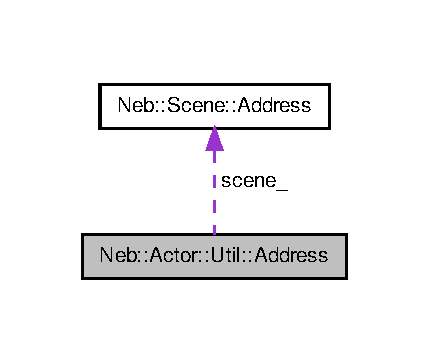
\includegraphics[width=210pt]{classNeb_1_1Actor_1_1Util_1_1Address__coll__graph}
\end{center}
\end{figure}
\subsection*{\-Public \-Member \-Functions}
\begin{DoxyCompactItemize}
\item 
\hypertarget{classNeb_1_1Actor_1_1Util_1_1Address_a888b40b0cd946b66bd3300d98d8edd0a}{void {\bfseries load\-\_\-this} (\-Neb\-::\-Actor\-::\-Base\-\_\-s const \&)}\label{classNeb_1_1Actor_1_1Util_1_1Address_a888b40b0cd946b66bd3300d98d8edd0a}

\item 
\hypertarget{classNeb_1_1Actor_1_1Util_1_1Address_a53a152cf8e0189b0afb2d2295c0886dc}{void {\bfseries load\-\_\-parent} (\-Neb\-::\-Actor\-::\-Base\-\_\-s const \&)}\label{classNeb_1_1Actor_1_1Util_1_1Address_a53a152cf8e0189b0afb2d2295c0886dc}

\item 
\hypertarget{classNeb_1_1Actor_1_1Util_1_1Address_ad128a12446aadf26c8aee1f0a6df36fc}{{\footnotesize template$<$class Archive $>$ }\\void {\bfseries serialize} (\-Archive \&ar, unsigned int const \&version)}\label{classNeb_1_1Actor_1_1Util_1_1Address_ad128a12446aadf26c8aee1f0a6df36fc}

\end{DoxyCompactItemize}
\subsection*{\-Public \-Attributes}
\begin{DoxyCompactItemize}
\item 
\hypertarget{classNeb_1_1Actor_1_1Util_1_1Address_a4b757419781a7ed7804556d50beee5cf}{\hyperlink{classNeb_1_1Scene_1_1Util_1_1Address}{\-Neb\-::\-Scene\-::\-Util\-::\-Address} {\bfseries scene\-\_\-}}\label{classNeb_1_1Actor_1_1Util_1_1Address_a4b757419781a7ed7804556d50beee5cf}

\item 
\hypertarget{classNeb_1_1Actor_1_1Util_1_1Address_aa9d6e45cf09caf8475a2ee6b6c79892b}{std\-::deque$<$ int $>$ {\bfseries vec\-\_\-}}\label{classNeb_1_1Actor_1_1Util_1_1Address_aa9d6e45cf09caf8475a2ee6b6c79892b}

\end{DoxyCompactItemize}


\-The documentation for this class was generated from the following files\-:\begin{DoxyCompactItemize}
\item 
src/\-Nebula/\-Actor/\-Util/\-Address.\-hh\item 
src/\-Nebula/\-Actor/\-Util/\-Address.\-cc\end{DoxyCompactItemize}

\hypertarget{classArchiveRead}{\section{Archive\-Read Class Reference}
\label{classArchiveRead}\index{Archive\-Read@{Archive\-Read}}
}
\subsection*{Public Member Functions}
\begin{DoxyCompactItemize}
\item 
\hypertarget{classArchiveRead_a776e35b241a26430d288a674454f032a}{{\footnotesize template$<$class A $>$ }\\\hyperlink{classArchiveRead}{Archive\-Read} \& {\bfseries operator\&} (A \&rhs)}\label{classArchiveRead_a776e35b241a26430d288a674454f032a}

\end{DoxyCompactItemize}


The documentation for this class was generated from the following file\-:\begin{DoxyCompactItemize}
\item 
src/\-Nebula/Archive.\-hh\end{DoxyCompactItemize}

\hypertarget{classNeb_1_1glsl_1_1attrib}{\section{\-Neb\-:\-:glsl\-:\-:attrib \-Class \-Reference}
\label{classNeb_1_1glsl_1_1attrib}\index{\-Neb\-::glsl\-::attrib@{\-Neb\-::glsl\-::attrib}}
}
\subsection*{\-Public \-Member \-Functions}
\begin{DoxyCompactItemize}
\item 
\hypertarget{classNeb_1_1glsl_1_1attrib_ad6cd70902fcafda280444fa1aed5d7f9}{void {\bfseries init} (char const $\ast$, \-G\-Luint)}\label{classNeb_1_1glsl_1_1attrib_ad6cd70902fcafda280444fa1aed5d7f9}

\item 
\hypertarget{classNeb_1_1glsl_1_1attrib_a3b71ba9f92059ba212b3fe9d95c2235d}{int {\bfseries locate} (std\-::shared\-\_\-ptr$<$ \hyperlink{classNeb_1_1glsl_1_1program}{\-Neb\-::glsl\-::program} $>$ p)}\label{classNeb_1_1glsl_1_1attrib_a3b71ba9f92059ba212b3fe9d95c2235d}

\item 
\hypertarget{classNeb_1_1glsl_1_1attrib_a787f4a60c290234fd0f6dc3b17df090c}{void {\bfseries enable} ()}\label{classNeb_1_1glsl_1_1attrib_a787f4a60c290234fd0f6dc3b17df090c}

\item 
\hypertarget{classNeb_1_1glsl_1_1attrib_a01fc89c183e17a5878e5bfc0ccc613c9}{void {\bfseries disable} ()}\label{classNeb_1_1glsl_1_1attrib_a01fc89c183e17a5878e5bfc0ccc613c9}

\end{DoxyCompactItemize}
\subsection*{\-Public \-Attributes}
\begin{DoxyCompactItemize}
\item 
\hypertarget{classNeb_1_1glsl_1_1attrib_ace010923299383f6c7f9023906597238}{char const $\ast$ {\bfseries name\-\_\-}}\label{classNeb_1_1glsl_1_1attrib_ace010923299383f6c7f9023906597238}

\item 
\hypertarget{classNeb_1_1glsl_1_1attrib_aa37e743b20a0e901d3274f4b88497195}{\-G\-Luint {\bfseries o\-\_\-}}\label{classNeb_1_1glsl_1_1attrib_aa37e743b20a0e901d3274f4b88497195}

\item 
\hypertarget{classNeb_1_1glsl_1_1attrib_acef1f0c5eb1de70001f4590e33eb9631}{\-G\-Luint {\bfseries o\-\_\-bind\-\_\-}}\label{classNeb_1_1glsl_1_1attrib_acef1f0c5eb1de70001f4590e33eb9631}

\end{DoxyCompactItemize}


\-The documentation for this class was generated from the following files\-:\begin{DoxyCompactItemize}
\item 
src/\-Nebula/\-Graphics/glsl/attrib.\-hpp\item 
src/\-Nebula/\-Graphics/glsl/attrib.\-cpp\end{DoxyCompactItemize}

\hypertarget{structNeb_1_1attrib__name}{\section{\-Neb\-:\-:attrib\-\_\-name \-Struct \-Reference}
\label{structNeb_1_1attrib__name}\index{\-Neb\-::attrib\-\_\-name@{\-Neb\-::attrib\-\_\-name}}
}
\subsection*{\-Public \-Types}
\begin{DoxyCompactItemize}
\item 
enum {\bfseries e} \{ \*
{\bfseries \-N\-O\-N\-E} =  0, 
{\bfseries \-P\-O\-S\-I\-T\-I\-O\-N}, 
{\bfseries \-N\-O\-R\-M\-A\-L}, 
{\bfseries \-T\-E\-X\-C\-O\-O\-R}, 
\*
{\bfseries \-C\-O\-O\-R}, 
{\bfseries \-C\-O\-O\-R}, 
{\bfseries \-T\-E\-X}, 
{\bfseries \-P\-O\-S\-I\-T\-I\-O\-N}, 
\*
{\bfseries \-N\-O\-R\-M\-A\-L}, 
{\bfseries \-T\-E\-X\-C\-O\-O\-R}
 \}
\item 
enum {\bfseries e} \{ \*
{\bfseries \-N\-O\-N\-E} =  0, 
{\bfseries \-P\-O\-S\-I\-T\-I\-O\-N}, 
{\bfseries \-N\-O\-R\-M\-A\-L}, 
{\bfseries \-T\-E\-X\-C\-O\-O\-R}, 
\*
{\bfseries \-C\-O\-O\-R}, 
{\bfseries \-C\-O\-O\-R}, 
{\bfseries \-T\-E\-X}, 
{\bfseries \-P\-O\-S\-I\-T\-I\-O\-N}, 
\*
{\bfseries \-N\-O\-R\-M\-A\-L}, 
{\bfseries \-T\-E\-X\-C\-O\-O\-R}
 \}
\end{DoxyCompactItemize}


\-The documentation for this struct was generated from the following files\-:\begin{DoxyCompactItemize}
\item 
src/\-Nebula/\-Enums.\-hh\item 
src/\-Nebula/\-Graphics/\-Types.\-hh\end{DoxyCompactItemize}

\hypertarget{classNeb_1_1Actor_1_1Control_1_1RigidBody_1_1Base}{\section{Neb\-:\-:Actor\-:\-:Control\-:\-:Rigid\-Body\-:\-:Base Class Reference}
\label{classNeb_1_1Actor_1_1Control_1_1RigidBody_1_1Base}\index{Neb\-::\-Actor\-::\-Control\-::\-Rigid\-Body\-::\-Base@{Neb\-::\-Actor\-::\-Control\-::\-Rigid\-Body\-::\-Base}}
}


Rigid Body An object (what did I mean by 'object' here, an actor?) makes no distinction between local and remote. In a remote scene, the actor will send a control update message. In a local scene, the actor will call upon stored values; it makes no difference to the actor whether these value were set by calls to key\-\_\-fun or by a control update message. This creates requirements for how control works. All infomation needed to determine force and torque at a given point in time must be stored in raw.  




{\ttfamily \#include $<$Base.\-hh$>$}



Inheritance diagram for Neb\-:\-:Actor\-:\-:Control\-:\-:Rigid\-Body\-:\-:Base\-:
\nopagebreak
\begin{figure}[H]
\begin{center}
\leavevmode
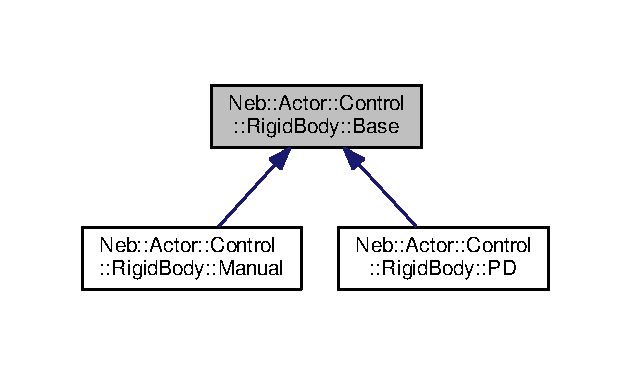
\includegraphics[width=303pt]{classNeb_1_1Actor_1_1Control_1_1RigidBody_1_1Base__inherit__graph}
\end{center}
\end{figure}
\subsection*{Public Member Functions}
\begin{DoxyCompactItemize}
\item 
\hypertarget{classNeb_1_1Actor_1_1Control_1_1RigidBody_1_1Base_aebd8b92d6ca5a4c8c3da4f421c7695bc}{virtual int {\bfseries key\-\_\-fun} (int, int, int, int)}\label{classNeb_1_1Actor_1_1Control_1_1RigidBody_1_1Base_aebd8b92d6ca5a4c8c3da4f421c7695bc}

\item 
\hypertarget{classNeb_1_1Actor_1_1Control_1_1RigidBody_1_1Base_a7f8b65567781b7441fd89df971caa403}{virtual void {\bfseries step} (double dt)=0}\label{classNeb_1_1Actor_1_1Control_1_1RigidBody_1_1Base_a7f8b65567781b7441fd89df971caa403}

\item 
\hypertarget{classNeb_1_1Actor_1_1Control_1_1RigidBody_1_1Base_aa1ce29a382717b1fb33b5010f9d26859}{virtual physx\-::\-Px\-Vec3 {\bfseries f} ()=0}\label{classNeb_1_1Actor_1_1Control_1_1RigidBody_1_1Base_aa1ce29a382717b1fb33b5010f9d26859}

\item 
\hypertarget{classNeb_1_1Actor_1_1Control_1_1RigidBody_1_1Base_abd9a7c8df4b02845027d970c94b70fdd}{virtual physx\-::\-Px\-Vec3 {\bfseries t} ()=0}\label{classNeb_1_1Actor_1_1Control_1_1RigidBody_1_1Base_abd9a7c8df4b02845027d970c94b70fdd}

\item 
\hypertarget{classNeb_1_1Actor_1_1Control_1_1RigidBody_1_1Base_a5a855eb91534056349e7a5c260bdbe5c}{void {\bfseries print} ()}\label{classNeb_1_1Actor_1_1Control_1_1RigidBody_1_1Base_a5a855eb91534056349e7a5c260bdbe5c}

\end{DoxyCompactItemize}
\subsection*{Public Attributes}
\begin{DoxyCompactItemize}
\item 
\hypertarget{classNeb_1_1Actor_1_1Control_1_1RigidBody_1_1Base_aba4c72bfcdf2119eeaa781f1a38fe772}{Neb\-::\-Actor\-::\-Base\-\_\-w {\bfseries actor\-\_\-}}\label{classNeb_1_1Actor_1_1Control_1_1RigidBody_1_1Base_aba4c72bfcdf2119eeaa781f1a38fe772}

\item 
\hypertarget{classNeb_1_1Actor_1_1Control_1_1RigidBody_1_1Base_ae9f74c25927f92c62f87ef4d913199f2}{physx\-::\-Px\-Quat {\bfseries q\-\_\-target\-\_\-}}\label{classNeb_1_1Actor_1_1Control_1_1RigidBody_1_1Base_ae9f74c25927f92c62f87ef4d913199f2}

\item 
\hypertarget{classNeb_1_1Actor_1_1Control_1_1RigidBody_1_1Base_a166bedae38ba63359842430dea3aa7c4}{physx\-::\-Px\-Vec3 {\bfseries p\-\_\-target\-\_\-}}\label{classNeb_1_1Actor_1_1Control_1_1RigidBody_1_1Base_a166bedae38ba63359842430dea3aa7c4}

\item 
\hypertarget{classNeb_1_1Actor_1_1Control_1_1RigidBody_1_1Base_a1d66da07350e4d4f40be39bb998ce1b3}{physx\-::\-Px\-Vec3 {\bfseries f\-\_\-}}\label{classNeb_1_1Actor_1_1Control_1_1RigidBody_1_1Base_a1d66da07350e4d4f40be39bb998ce1b3}

\item 
\hypertarget{classNeb_1_1Actor_1_1Control_1_1RigidBody_1_1Base_a3d8f432f431e924ba55fdf0c379941cb}{physx\-::\-Px\-Vec3 {\bfseries t\-\_\-}}\label{classNeb_1_1Actor_1_1Control_1_1RigidBody_1_1Base_a3d8f432f431e924ba55fdf0c379941cb}

\item 
\hypertarget{classNeb_1_1Actor_1_1Control_1_1RigidBody_1_1Base_ac29d5340c75af4aaede80287f6f133bd}{physx\-::\-Px\-Vec3 {\bfseries force\-\_\-}}\label{classNeb_1_1Actor_1_1Control_1_1RigidBody_1_1Base_ac29d5340c75af4aaede80287f6f133bd}

\item 
\hypertarget{classNeb_1_1Actor_1_1Control_1_1RigidBody_1_1Base_ac4b7640c016cd84cf4598ce32fadb8f4}{physx\-::\-Px\-Vec3 {\bfseries torque\-\_\-}}\label{classNeb_1_1Actor_1_1Control_1_1RigidBody_1_1Base_ac4b7640c016cd84cf4598ce32fadb8f4}

\item 
\hypertarget{classNeb_1_1Actor_1_1Control_1_1RigidBody_1_1Base_a7663ba3daf78f37297e094b279f513db}{\begin{tabbing}
xx\=xx\=xx\=xx\=xx\=xx\=xx\=xx\=xx\=\kill
struct \{\\
\hypertarget{structNeb_1_1Actor_1_1Control_1_1RigidBody_1_1Base_1_1@1_a9f7f3fdadbfac948f6a8d7fdc64d77a2}{\>boost::signals2::connection {\bfseries key\_fun\_}\\
\} {\bfseries conn\_}}\label{classNeb_1_1Actor_1_1Control_1_1RigidBody_1_1Base_a7663ba3daf78f37297e094b279f513db}
\\

\end{tabbing}\end{DoxyCompactItemize}


\subsection{Detailed Description}
Rigid Body An object (what did I mean by 'object' here, an actor?) makes no distinction between local and remote. In a remote scene, the actor will send a control update message. In a local scene, the actor will call upon stored values; it makes no difference to the actor whether these value were set by calls to key\-\_\-fun or by a control update message. This creates requirements for how control works. All infomation needed to determine force and torque at a given point in time must be stored in raw. 

The documentation for this class was generated from the following files\-:\begin{DoxyCompactItemize}
\item 
src/\-Nebula/\-Actor/\-Control/\-Rigid\-Body/Base.\-hh\item 
src/\-Nebula/\-Actor/\-Control/\-Rigid\-Body/Base.\-cc\end{DoxyCompactItemize}

\hypertarget{classgal_1_1network_1_1base}{\section{gal\-:\-:network\-:\-:base \-Class \-Reference}
\label{classgal_1_1network_1_1base}\index{gal\-::network\-::base@{gal\-::network\-::base}}
}


\-Inheritance diagram for gal\-:\-:network\-:\-:base\-:
\nopagebreak
\begin{figure}[H]
\begin{center}
\leavevmode
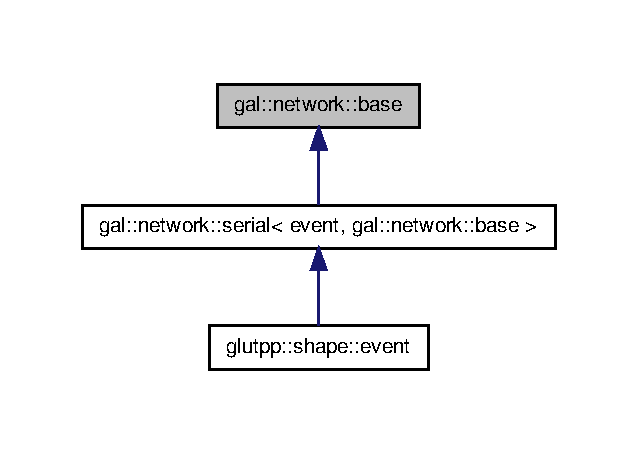
\includegraphics[width=306pt]{classgal_1_1network_1_1base__inherit__graph}
\end{center}
\end{figure}


\-The documentation for this class was generated from the following file\-:\begin{DoxyCompactItemize}
\item 
src/gru/network/serial.\-hpp\end{DoxyCompactItemize}

\hypertarget{classNeb_1_1App_1_1Base}{\section{\-Neb\-:\-:\-App\-:\-:\-Base \-Class \-Reference}
\label{classNeb_1_1App_1_1Base}\index{\-Neb\-::\-App\-::\-Base@{\-Neb\-::\-App\-::\-Base}}
}


\-Inheritance diagram for \-Neb\-:\-:\-App\-:\-:\-Base\-:\nopagebreak
\begin{figure}[H]
\begin{center}
\leavevmode
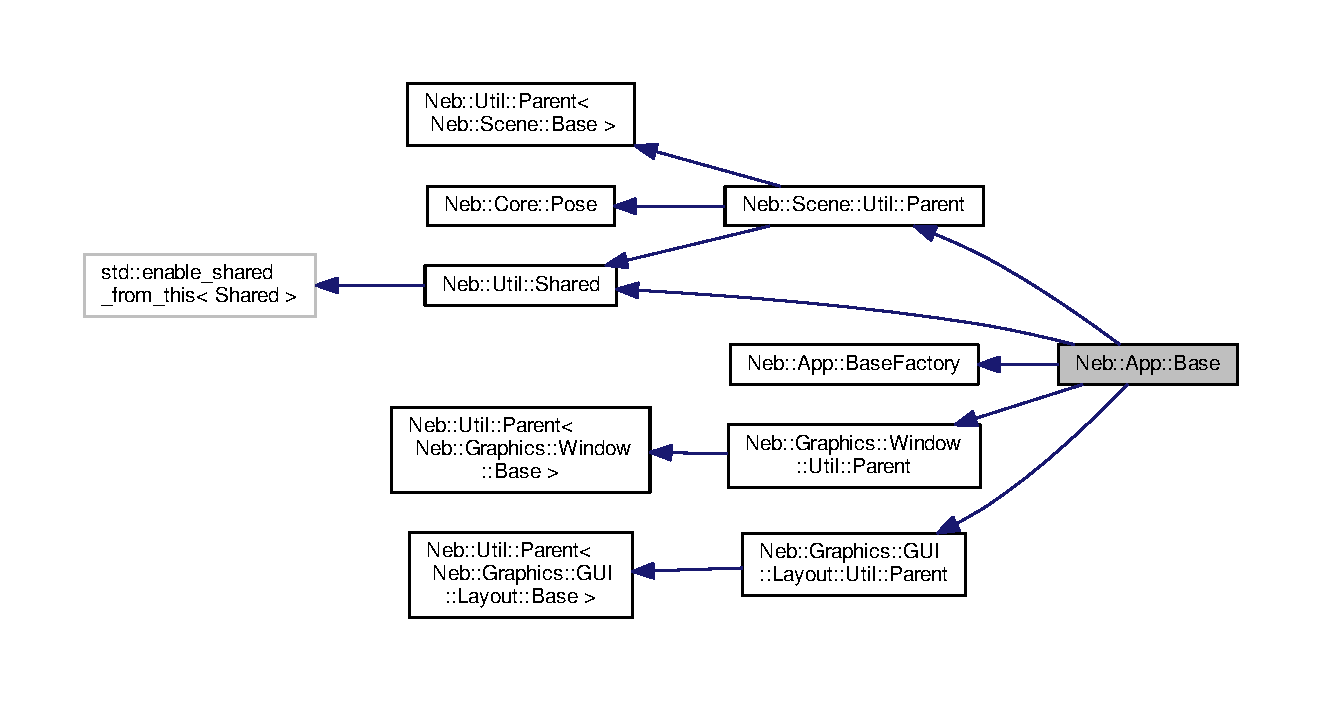
\includegraphics[width=350pt]{classNeb_1_1App_1_1Base__inherit__graph}
\end{center}
\end{figure}


\-Collaboration diagram for \-Neb\-:\-:\-App\-:\-:\-Base\-:\nopagebreak
\begin{figure}[H]
\begin{center}
\leavevmode
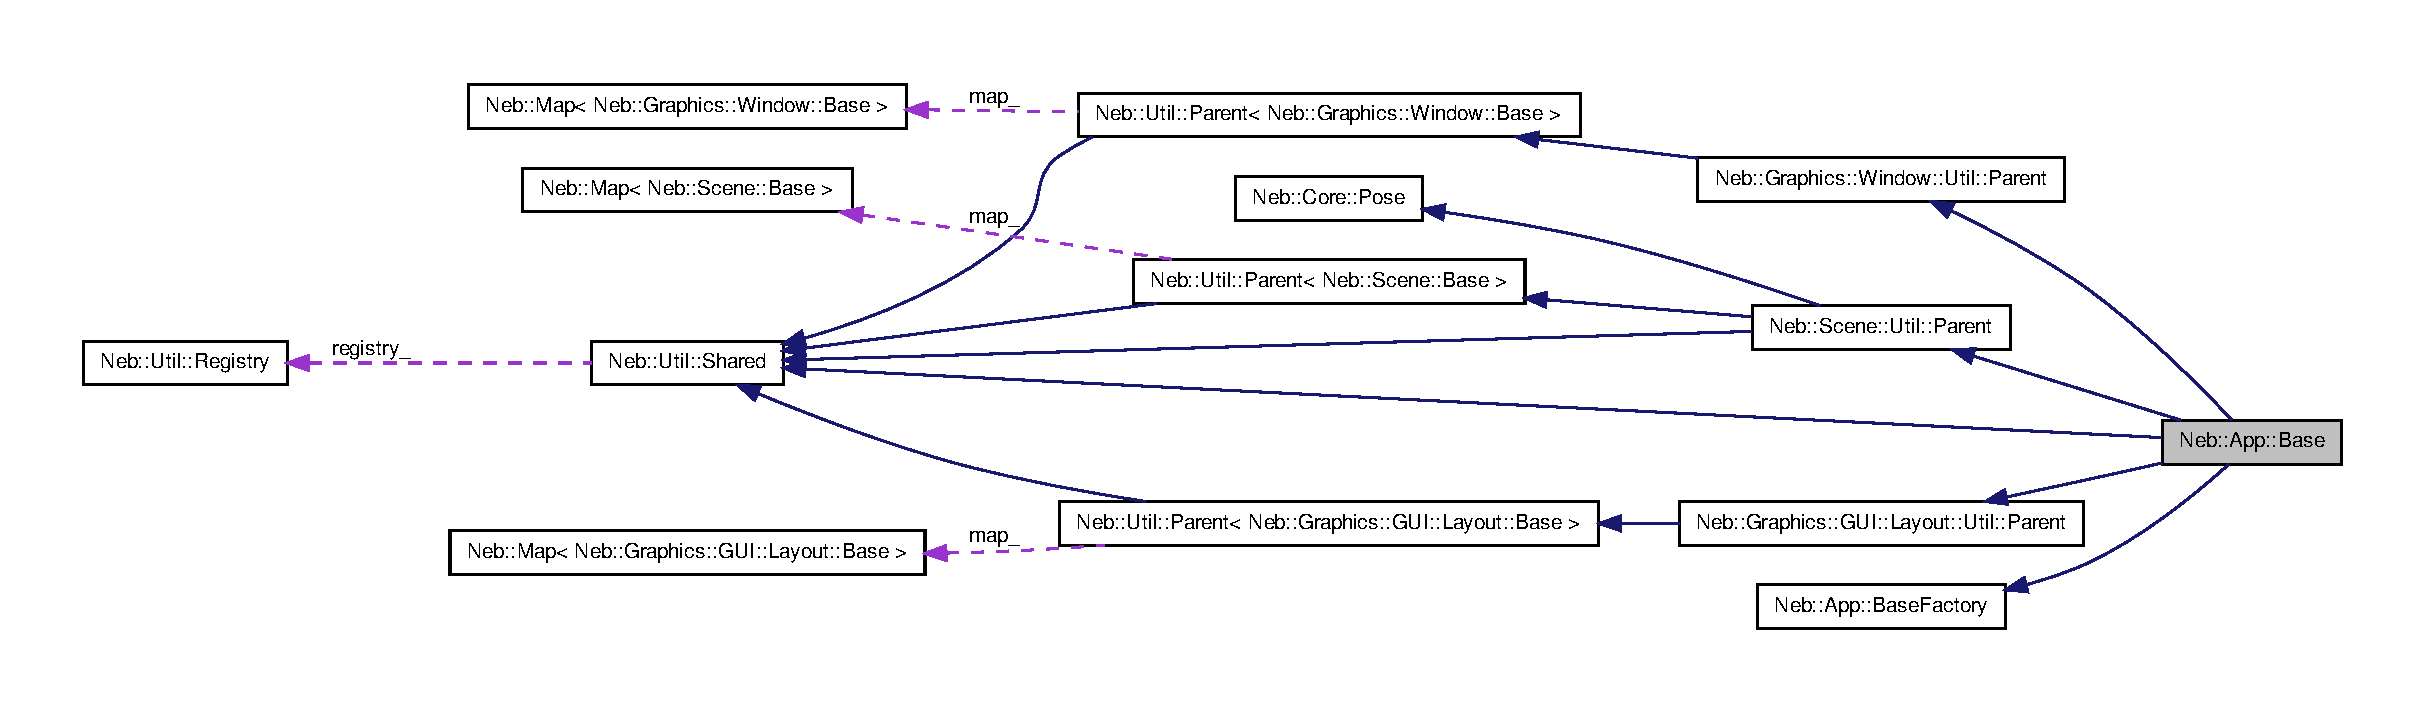
\includegraphics[width=350pt]{classNeb_1_1App_1_1Base__coll__graph}
\end{center}
\end{figure}
\subsection*{\-Classes}
\begin{DoxyCompactItemize}
\item 
struct \hyperlink{structNeb_1_1App_1_1Base_1_1flag}{flag}
\end{DoxyCompactItemize}
\subsection*{\-Public \-Types}
\begin{DoxyCompactItemize}
\item 
\hypertarget{classNeb_1_1App_1_1Base_a893ad32232e1d5607f16c0a8712e2742}{typedef std\-::map$<$ \-G\-L\-F\-Wwindow \*
$\ast$, \-Neb\-::\-Graphics\-::\-Window\-::\-Base\-\_\-s $>$ {\bfseries glfwwindow\-\_\-map\-\_\-type}}\label{classNeb_1_1App_1_1Base_a893ad32232e1d5607f16c0a8712e2742}

\end{DoxyCompactItemize}
\subsection*{\-Public \-Member \-Functions}
\begin{DoxyCompactItemize}
\item 
\hypertarget{classNeb_1_1App_1_1Base_add6e387b326940dc524ed6cd9d5d76db}{void {\bfseries command} (std\-::string)}\label{classNeb_1_1App_1_1Base_add6e387b326940dc524ed6cd9d5d76db}

\item 
\hypertarget{classNeb_1_1App_1_1Base_ad1b379ac9a17366de1f53859fdf56eff}{std\-::shared\-\_\-ptr\*
$<$ \hyperlink{classNeb_1_1glsl_1_1program}{\-Neb\-::glsl\-::program} $>$ {\bfseries use\-\_\-program} (\-Neb\-::program\-\_\-name\-::e)}\label{classNeb_1_1App_1_1Base_ad1b379ac9a17366de1f53859fdf56eff}

\item 
\hypertarget{classNeb_1_1App_1_1Base_a87ec2d1ee35f0a54746b445400d09da0}{std\-::shared\-\_\-ptr\*
$<$ \hyperlink{classNeb_1_1glsl_1_1program}{\-Neb\-::glsl\-::program} $>$ {\bfseries get\-\_\-program} (\-Neb\-::program\-\_\-name\-::e)}\label{classNeb_1_1App_1_1Base_a87ec2d1ee35f0a54746b445400d09da0}

\item 
\hypertarget{classNeb_1_1App_1_1Base_afb7f83fe4804b67c2ec09980f012bf24}{std\-::shared\-\_\-ptr\*
$<$ \hyperlink{classNeb_1_1glsl_1_1program}{\-Neb\-::glsl\-::program} $>$ {\bfseries current\-\_\-program} ()}\label{classNeb_1_1App_1_1Base_afb7f83fe4804b67c2ec09980f012bf24}

\item 
\hypertarget{classNeb_1_1App_1_1Base_a8aaee8b061c48ae6eeb997bf9393aa62}{void {\bfseries create\-\_\-programs} ()}\label{classNeb_1_1App_1_1Base_a8aaee8b061c48ae6eeb997bf9393aa62}

\item 
\hypertarget{classNeb_1_1App_1_1Base_a7cbbae817434580b497ace5b6afb6283}{physx\-::\-Px\-Transform {\bfseries get\-Pose} ()}\label{classNeb_1_1App_1_1Base_a7cbbae817434580b497ace5b6afb6283}

\item 
\hypertarget{classNeb_1_1App_1_1Base_a3cd18fcee50a8fb487155f7bb9822d97}{physx\-::\-Px\-Transform {\bfseries get\-Pose\-Global} ()}\label{classNeb_1_1App_1_1Base_a3cd18fcee50a8fb487155f7bb9822d97}

\item 
\hypertarget{classNeb_1_1App_1_1Base_a3c200a59a2141594b8ad6adcb6e8b7c9}{\-Neb\-::\-Graphics\-::\-Window\-::\-Base\-\_\-s {\bfseries get\-\_\-window} (\-G\-L\-F\-Wwindow $\ast$)}\label{classNeb_1_1App_1_1Base_a3c200a59a2141594b8ad6adcb6e8b7c9}

\item 
\hypertarget{classNeb_1_1App_1_1Base_a45b4feac51086c0b894eb2e30ea98e03}{\-G\-L\-F\-Wwindow $\ast$ {\bfseries reg} (\-Neb\-::\-Graphics\-::\-Window\-::\-Base\-\_\-s)}\label{classNeb_1_1App_1_1Base_a45b4feac51086c0b894eb2e30ea98e03}

\item 
\hypertarget{classNeb_1_1App_1_1Base_a7872dfc7dbb8cd5a2d53326db38076cb}{void {\bfseries init} ()}\label{classNeb_1_1App_1_1Base_a7872dfc7dbb8cd5a2d53326db38076cb}

\item 
\hypertarget{classNeb_1_1App_1_1Base_a54df5d224b6b7fe039ffb5805be8460b}{void {\bfseries load\-\_\-layout} (int, char const $\ast$)}\label{classNeb_1_1App_1_1Base_a54df5d224b6b7fe039ffb5805be8460b}

\item 
\hypertarget{classNeb_1_1App_1_1Base_af1be18f5e33e09cd193ea159b75bff70}{int {\bfseries step} (double)}\label{classNeb_1_1App_1_1Base_af1be18f5e33e09cd193ea159b75bff70}

\item 
\hypertarget{classNeb_1_1App_1_1Base_a126da4ec133d3e67e06bc16c962a5aac}{int {\bfseries loop} ()}\label{classNeb_1_1App_1_1Base_a126da4ec133d3e67e06bc16c962a5aac}

\item 
\hypertarget{classNeb_1_1App_1_1Base_a3a0d4a61b10740915bd60fb24c607fea}{void {\bfseries set\-\_\-should\-\_\-release} ()}\label{classNeb_1_1App_1_1Base_a3a0d4a61b10740915bd60fb24c607fea}

\item 
\hypertarget{classNeb_1_1App_1_1Base_a495ad0c7fade8667358ae93bf8d193ef}{int {\bfseries activate\-\_\-scene} (int, int)}\label{classNeb_1_1App_1_1Base_a495ad0c7fade8667358ae93bf8d193ef}

\item 
\hypertarget{classNeb_1_1App_1_1Base_ac695c0ce0790177af0a8e8560a8368be}{int {\bfseries deactivate\-\_\-scene} (int)}\label{classNeb_1_1App_1_1Base_ac695c0ce0790177af0a8e8560a8368be}

\item 
\hypertarget{classNeb_1_1App_1_1Base_a2c15bc36fb6d54115396c83d07c1ed4e}{int {\bfseries activate\-\_\-layout} (int, int)}\label{classNeb_1_1App_1_1Base_a2c15bc36fb6d54115396c83d07c1ed4e}

\item 
\hypertarget{classNeb_1_1App_1_1Base_a8569d504264c9473c32cec6f21399839}{int {\bfseries deactivate\-\_\-layout} (int)}\label{classNeb_1_1App_1_1Base_a8569d504264c9473c32cec6f21399839}

\end{DoxyCompactItemize}
\begin{Indent}{\bf \-Serialization @\{}\par
\begin{DoxyCompactItemize}
\item 
\hypertarget{classNeb_1_1App_1_1Base_aef5b0330ea53ea1ed0701cc86f0a6e02}{{\footnotesize template$<$class A $>$ }\\void {\bfseries load\-Xml} (std\-::string filename, \-A \&a)}\label{classNeb_1_1App_1_1Base_aef5b0330ea53ea1ed0701cc86f0a6e02}

\end{DoxyCompactItemize}
\end{Indent}
\begin{Indent}{\bf \-Search @\{}\par
\begin{DoxyCompactItemize}
\item 
\hypertarget{classNeb_1_1App_1_1Base_ab15cef6932ba3060d20244d65034e456}{\-Neb\-::\-Actor\-::\-Base\-\_\-w {\bfseries get\-Actor} (\hyperlink{classNeb_1_1Actor_1_1Util_1_1Address}{\-Neb\-::\-Actor\-::\-Util\-::\-Address})}\label{classNeb_1_1App_1_1Base_ab15cef6932ba3060d20244d65034e456}

\end{DoxyCompactItemize}
\end{Indent}
\begin{Indent}{\bf \-Network @\{}\par
\begin{DoxyCompactItemize}
\item 
\hypertarget{classNeb_1_1App_1_1Base_ab9d0a601ee3d27fdde0ae749688301bc}{void {\bfseries reset\-\_\-server} (unsigned short)}\label{classNeb_1_1App_1_1Base_ab9d0a601ee3d27fdde0ae749688301bc}

\item 
\hypertarget{classNeb_1_1App_1_1Base_a7dbb058185e79e6d9766c5bcba10ef94}{void {\bfseries reset\-\_\-client} (char const $\ast$, unsigned short)}\label{classNeb_1_1App_1_1Base_a7dbb058185e79e6d9766c5bcba10ef94}

\item 
\hypertarget{classNeb_1_1App_1_1Base_a63794136246ca794a014bc89f93b8da0}{void {\bfseries send\-\_\-server} (gal\-::network\-::omessage\-\_\-s)}\label{classNeb_1_1App_1_1Base_a63794136246ca794a014bc89f93b8da0}

\item 
\hypertarget{classNeb_1_1App_1_1Base_a01f7c70061935f52d5c60ec4ee568187}{void {\bfseries send\-\_\-client} (gal\-::network\-::omessage\-\_\-s)}\label{classNeb_1_1App_1_1Base_a01f7c70061935f52d5c60ec4ee568187}

\item 
\hypertarget{classNeb_1_1App_1_1Base_a9e6d3043a77d97af9f7cbe326071c49d}{int {\bfseries transmit\-\_\-scenes} (\-Neb\-::\-Network\-::\-Communicating\-\_\-s)}\label{classNeb_1_1App_1_1Base_a9e6d3043a77d97af9f7cbe326071c49d}

\end{DoxyCompactItemize}
\end{Indent}
\subsection*{\-Static \-Public \-Member \-Functions}
\begin{Indent}{\bf \-Accessors @\{}\par
\begin{DoxyCompactItemize}
\item 
\hypertarget{classNeb_1_1App_1_1Base_a07fbe923b685fd30e7a9e34473a8b67f}{static \-Neb\-::\-App\-::\-Base\-\_\-s {\bfseries global\-Base} ()}\label{classNeb_1_1App_1_1Base_a07fbe923b685fd30e7a9e34473a8b67f}

\end{DoxyCompactItemize}
\end{Indent}
\subsection*{\-Public \-Attributes}
\begin{Indent}{\bf \-Font @\{}\par
\begin{DoxyCompactItemize}
\item 
\hypertarget{classNeb_1_1App_1_1Base_a957424f530de5476709d7046653d7567}{\-F\-T\-\_\-\-Library {\bfseries ft\-\_\-}}\label{classNeb_1_1App_1_1Base_a957424f530de5476709d7046653d7567}

\end{DoxyCompactItemize}
\end{Indent}
\begin{Indent}{\bf \-Boost \-Asio @\{}\par
\begin{DoxyCompactItemize}
\item 
\hypertarget{classNeb_1_1App_1_1Base_a99c95783c97c8e34ad2fafd1806367e2}{boost\-::asio\-::io\-\_\-service {\bfseries ios\-\_\-}}\label{classNeb_1_1App_1_1Base_a99c95783c97c8e34ad2fafd1806367e2}

\end{DoxyCompactItemize}
\end{Indent}
\subsection*{\-Static \-Private \-Member \-Functions}
\begin{DoxyCompactItemize}
\item 
\hypertarget{classNeb_1_1App_1_1Base_a93845fd33edaa8147bc2c434bd659319}{static void {\bfseries static\-\_\-error\-\_\-fun} (int, char const $\ast$)}\label{classNeb_1_1App_1_1Base_a93845fd33edaa8147bc2c434bd659319}

\item 
\hypertarget{classNeb_1_1App_1_1Base_a7c514e4d4f961562a23470746e0c1e5f}{static void {\bfseries static\-\_\-window\-\_\-pos\-\_\-fun} (\-G\-L\-F\-Wwindow $\ast$, int, int)}\label{classNeb_1_1App_1_1Base_a7c514e4d4f961562a23470746e0c1e5f}

\item 
\hypertarget{classNeb_1_1App_1_1Base_ac6ebbd8d1fba3df2be6703da827664e9}{static void {\bfseries static\-\_\-window\-\_\-size\-\_\-fun} (\-G\-L\-F\-Wwindow $\ast$, int, int)}\label{classNeb_1_1App_1_1Base_ac6ebbd8d1fba3df2be6703da827664e9}

\item 
\hypertarget{classNeb_1_1App_1_1Base_a00b301462b513b106c215d700c4954b8}{static void {\bfseries static\-\_\-window\-\_\-close\-\_\-fun} (\-G\-L\-F\-Wwindow $\ast$)}\label{classNeb_1_1App_1_1Base_a00b301462b513b106c215d700c4954b8}

\item 
\hypertarget{classNeb_1_1App_1_1Base_ad1a134d03f2c5bea0e121409319288ef}{static void {\bfseries static\-\_\-window\-\_\-refresh\-\_\-fun} (\-G\-L\-F\-Wwindow $\ast$)}\label{classNeb_1_1App_1_1Base_ad1a134d03f2c5bea0e121409319288ef}

\item 
\hypertarget{classNeb_1_1App_1_1Base_a9b852739b48f0a9673e683a8b1dc564a}{static void {\bfseries static\-\_\-mouse\-\_\-button\-\_\-fun} (\-G\-L\-F\-Wwindow $\ast$, int, int, int)}\label{classNeb_1_1App_1_1Base_a9b852739b48f0a9673e683a8b1dc564a}

\item 
\hypertarget{classNeb_1_1App_1_1Base_a924384d0558f9d7caf79154e31e755a5}{static void {\bfseries static\-\_\-key\-\_\-fun} (\-G\-L\-F\-Wwindow $\ast$, int, int, int, int)}\label{classNeb_1_1App_1_1Base_a924384d0558f9d7caf79154e31e755a5}

\end{DoxyCompactItemize}
\subsection*{\-Private \-Attributes}
\begin{DoxyCompactItemize}
\item 
\-Neb\-::\-Network\-::\-Server\-\_\-s \hyperlink{classNeb_1_1App_1_1Base_a347da33116990d3f31246d0d09b520bb}{server\-\_\-}
\item 
\hypertarget{classNeb_1_1App_1_1Base_a61762bbdfc8de4eda705593de4446f90}{\-Neb\-::\-Network\-::\-Client\-\_\-s {\bfseries client\-\_\-}}\label{classNeb_1_1App_1_1Base_a61762bbdfc8de4eda705593de4446f90}

\item 
\hypertarget{classNeb_1_1App_1_1Base_a1e9ceef6134c7988724583a3382c4ce9}{\-Neb\-::\-App\-::\-Util\-::\-Flag {\bfseries flag\-\_\-}}\label{classNeb_1_1App_1_1Base_a1e9ceef6134c7988724583a3382c4ce9}

\item 
\hypertarget{classNeb_1_1App_1_1Base_ada7720dc61c7709cd07495d68d686027}{glfwwindow\-\_\-map\-\_\-type {\bfseries windows\-\_\-glfw\-\_\-}}\label{classNeb_1_1App_1_1Base_ada7720dc61c7709cd07495d68d686027}

\item 
\hypertarget{classNeb_1_1App_1_1Base_a33e8d1e662c649ee561e94a9ca486ef9}{std\-::map$<$ int, std\-::shared\-\_\-ptr\*
$<$ \hyperlink{classNeb_1_1glsl_1_1program}{\-Neb\-::glsl\-::program} $>$ $>$ {\bfseries programs\-\_\-}}\label{classNeb_1_1App_1_1Base_a33e8d1e662c649ee561e94a9ca486ef9}

\item 
\hypertarget{classNeb_1_1App_1_1Base_aa754357debda8debd26b78ff8d01a97f}{std\-::shared\-\_\-ptr\*
$<$ \hyperlink{classNeb_1_1glsl_1_1program}{\-Neb\-::glsl\-::program} $>$ {\bfseries current\-\_\-}}\label{classNeb_1_1App_1_1Base_aa754357debda8debd26b78ff8d01a97f}

\end{DoxyCompactItemize}
\subsection*{\-Static \-Private \-Attributes}
\begin{DoxyCompactItemize}
\item 
static \*
\-Neb\-::\-Graphics\-::\-Window\-::\-Base\-\_\-w \hyperlink{classNeb_1_1App_1_1Base_a4a6527469072e5d1f01f76215b6b2fd3}{window\-\_\-main\-\_\-}
\end{DoxyCompactItemize}


\subsection{\-Member \-Data \-Documentation}
\hypertarget{classNeb_1_1App_1_1Base_a347da33116990d3f31246d0d09b520bb}{\index{\-Neb\-::\-App\-::\-Base@{\-Neb\-::\-App\-::\-Base}!server\-\_\-@{server\-\_\-}}
\index{server\-\_\-@{server\-\_\-}!Neb::App::Base@{\-Neb\-::\-App\-::\-Base}}
\subsubsection[{server\-\_\-}]{\setlength{\rightskip}{0pt plus 5cm}\-Neb\-::\-Network\-::\-Server\-\_\-s {\bf \-Neb\-::\-App\-::\-Base\-::server\-\_\-}\hspace{0.3cm}{\ttfamily  \mbox{[}private\mbox{]}}}}\label{classNeb_1_1App_1_1Base_a347da33116990d3f31246d0d09b520bb}
\begin{DoxyRefDesc}{\-Todo}
\item[\hyperlink{todo__todo000007}{\-Todo}]make derived \-App classes for \-Server and \-Client??? \end{DoxyRefDesc}
\hypertarget{classNeb_1_1App_1_1Base_a4a6527469072e5d1f01f76215b6b2fd3}{\index{\-Neb\-::\-App\-::\-Base@{\-Neb\-::\-App\-::\-Base}!window\-\_\-main\-\_\-@{window\-\_\-main\-\_\-}}
\index{window\-\_\-main\-\_\-@{window\-\_\-main\-\_\-}!Neb::App::Base@{\-Neb\-::\-App\-::\-Base}}
\subsubsection[{window\-\_\-main\-\_\-}]{\setlength{\rightskip}{0pt plus 5cm}\-Neb\-::\-Graphics\-::\-Window\-::\-Base\-\_\-w {\bf \-Neb\-::\-App\-::\-Base\-::window\-\_\-main\-\_\-}\hspace{0.3cm}{\ttfamily  \mbox{[}static, private\mbox{]}}}}\label{classNeb_1_1App_1_1Base_a4a6527469072e5d1f01f76215b6b2fd3}
\begin{DoxyRefDesc}{\-Todo}
\item[\hyperlink{todo__todo000006}{\-Todo}]since std smart pointers dont have ref counted unique pointers, owned objects must be stored as shared pointers. to avoid unwanted shared\-\_\-ptrs to owned objects, care must be taken when passing these objects around. better documentation inside function bodies should be used to let me know what a shared\-\_\-ptr is being used (how it should be treated. \end{DoxyRefDesc}


\-The documentation for this class was generated from the following files\-:\begin{DoxyCompactItemize}
\item 
src/\-Nebula/\-App/\-Base.\-hh\item 
src/\-Nebula/\-App/\-Base.\-cc\end{DoxyCompactItemize}

\hypertarget{classNeb_1_1Actor_1_1RigidBody_1_1Base}{\section{Neb\-:\-:Actor\-:\-:Rigid\-Body\-:\-:Base Class Reference}
\label{classNeb_1_1Actor_1_1RigidBody_1_1Base}\index{Neb\-::\-Actor\-::\-Rigid\-Body\-::\-Base@{Neb\-::\-Actor\-::\-Rigid\-Body\-::\-Base}}
}


Inheritance diagram for Neb\-:\-:Actor\-:\-:Rigid\-Body\-:\-:Base\-:
\nopagebreak
\begin{figure}[H]
\begin{center}
\leavevmode
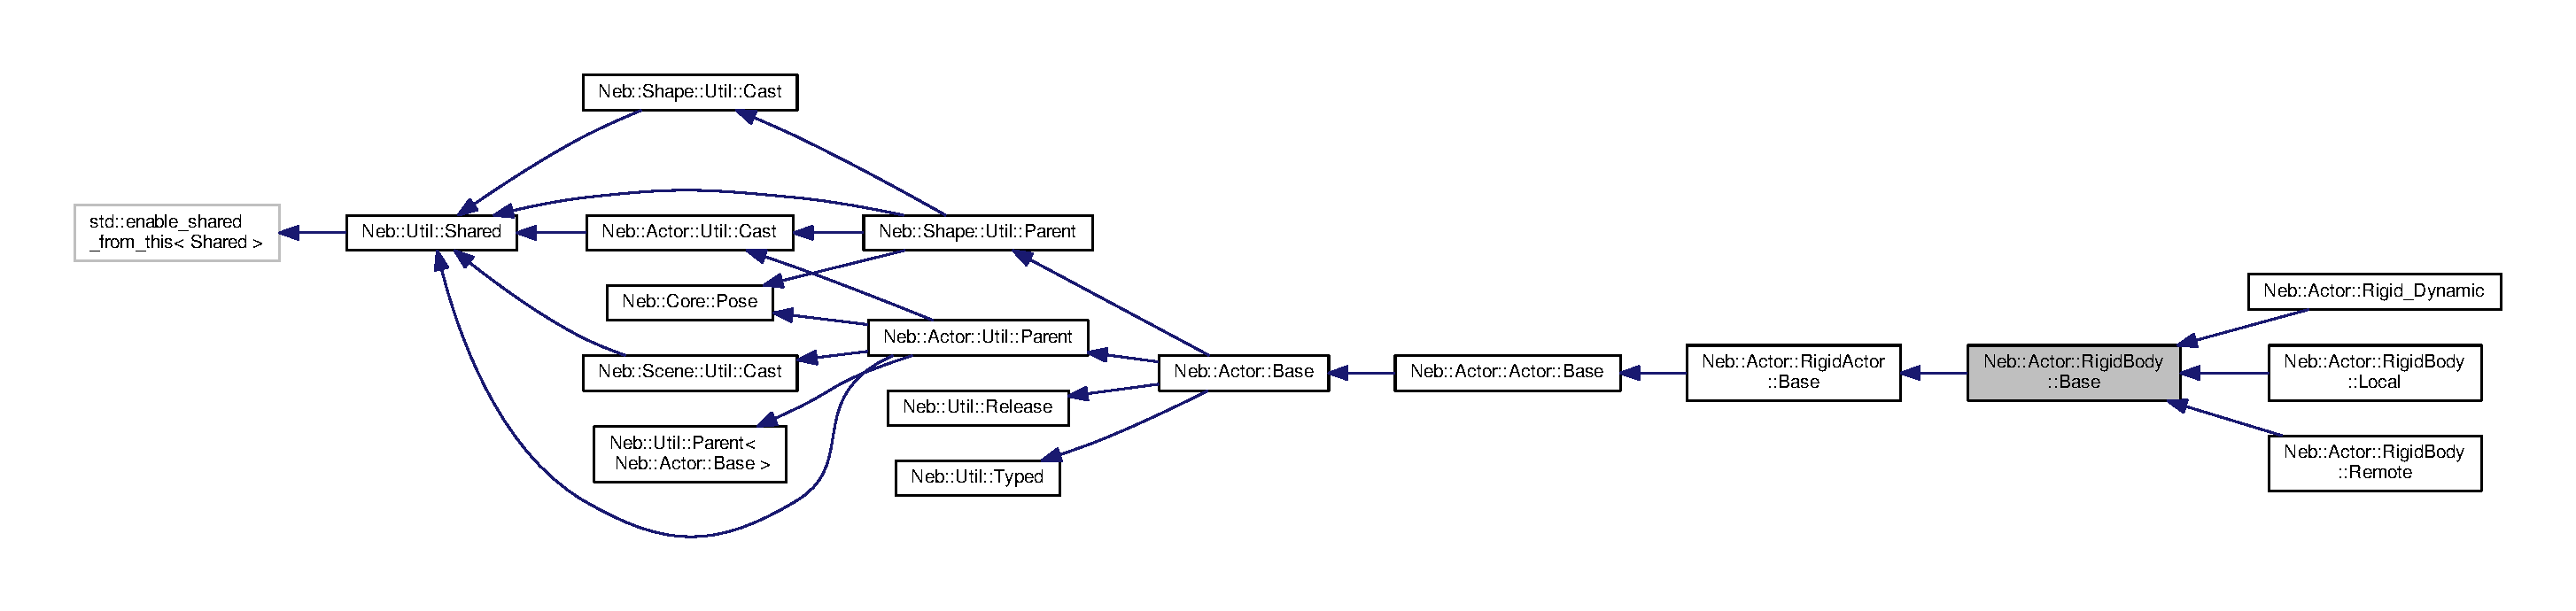
\includegraphics[width=350pt]{classNeb_1_1Actor_1_1RigidBody_1_1Base__inherit__graph}
\end{center}
\end{figure}


Collaboration diagram for Neb\-:\-:Actor\-:\-:Rigid\-Body\-:\-:Base\-:
\nopagebreak
\begin{figure}[H]
\begin{center}
\leavevmode
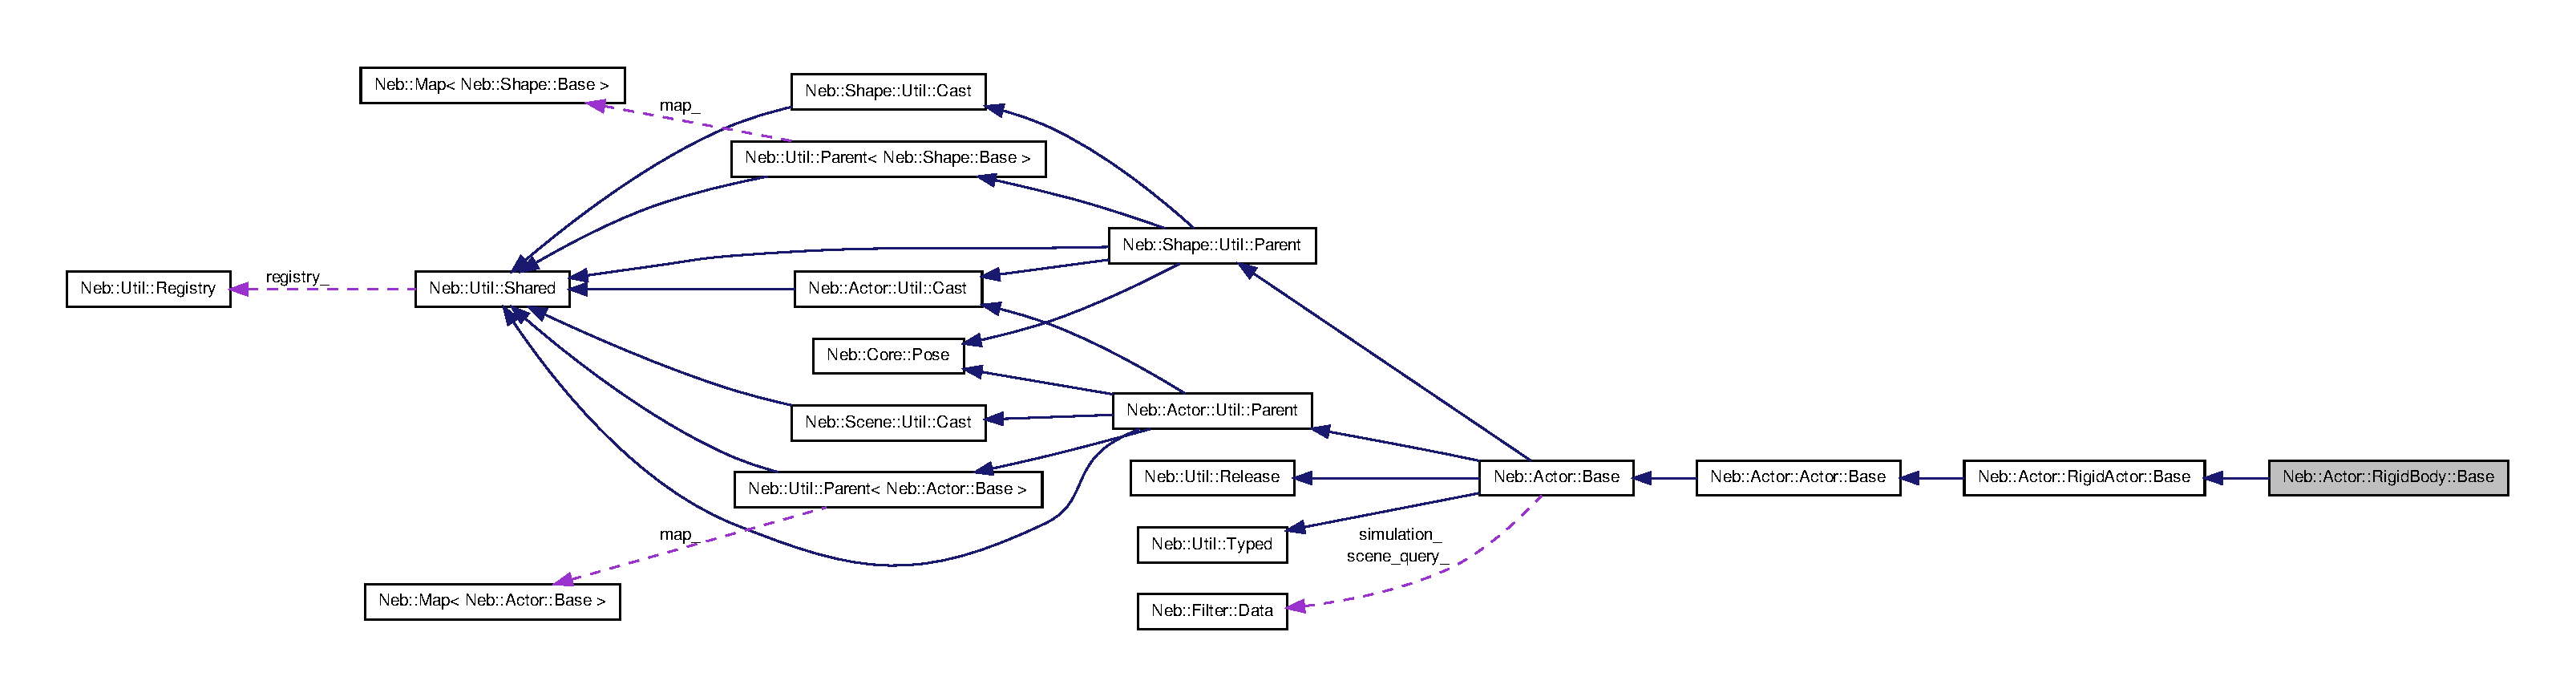
\includegraphics[width=350pt]{classNeb_1_1Actor_1_1RigidBody_1_1Base__coll__graph}
\end{center}
\end{figure}
\subsection*{Public Member Functions}
\begin{DoxyCompactItemize}
\item 
\hypertarget{classNeb_1_1Actor_1_1RigidBody_1_1Base_ae20c50935510fa8d3eee87010da087a0}{{\bfseries Base} (Neb\-::\-Actor\-::\-Util\-::\-Parent\-\_\-s)}\label{classNeb_1_1Actor_1_1RigidBody_1_1Base_ae20c50935510fa8d3eee87010da087a0}

\item 
\hypertarget{classNeb_1_1Actor_1_1RigidBody_1_1Base_af3732712c0867fa7fa3c4d57442d6e99}{virtual void {\bfseries init} ()}\label{classNeb_1_1Actor_1_1RigidBody_1_1Base_af3732712c0867fa7fa3c4d57442d6e99}

\item 
\hypertarget{classNeb_1_1Actor_1_1RigidBody_1_1Base_ac01f0719fc0af06f286a89f6805e3c82}{virtual Neb\-::\-Actor\-::\-Base\-\_\-s {\bfseries get\-\_\-projectile} ()}\label{classNeb_1_1Actor_1_1RigidBody_1_1Base_ac01f0719fc0af06f286a89f6805e3c82}

\item 
\hypertarget{classNeb_1_1Actor_1_1RigidBody_1_1Base_a94184455c508f43845009606f70b9d7f}{virtual void {\bfseries print\-\_\-info} ()}\label{classNeb_1_1Actor_1_1RigidBody_1_1Base_a94184455c508f43845009606f70b9d7f}

\item 
\hypertarget{classNeb_1_1Actor_1_1RigidBody_1_1Base_a8c59f06c4487432769c93566f01b81dd}{virtual void {\bfseries create\-\_\-physics} ()=0}\label{classNeb_1_1Actor_1_1RigidBody_1_1Base_a8c59f06c4487432769c93566f01b81dd}

\item 
\hypertarget{classNeb_1_1Actor_1_1RigidBody_1_1Base_a13dd372df1d14fb3d8502d8b4c7a9528}{void {\bfseries set\-Control} (Neb\-::\-Actor\-::\-Control\-::\-Rigid\-Body\-::\-Base\-\_\-s)}\label{classNeb_1_1Actor_1_1RigidBody_1_1Base_a13dd372df1d14fb3d8502d8b4c7a9528}

\end{DoxyCompactItemize}
\subsection*{Public Attributes}
\begin{DoxyCompactItemize}
\item 
\hypertarget{classNeb_1_1Actor_1_1RigidBody_1_1Base_a2de60916961ec44a1c4f6781a8f25a52}{Neb\-::\-Actor\-::\-Control\-::\-Rigid\-Body\-::\-Base\-\_\-s {\bfseries control\-\_\-}}\label{classNeb_1_1Actor_1_1RigidBody_1_1Base_a2de60916961ec44a1c4f6781a8f25a52}

\end{DoxyCompactItemize}
\subsection*{Additional Inherited Members}


The documentation for this class was generated from the following file\-:\begin{DoxyCompactItemize}
\item 
src/\-Nebula/\-Actor/rigid\-\_\-body/rigid\-\_\-body.\-hh\end{DoxyCompactItemize}

\hypertarget{classNeb_1_1glsl_1_1Uniform_1_1Vector_1_1Base}{\section{Neb\-:\-:glsl\-:\-:Uniform\-:\-:Vector\-:\-:Base Class Reference}
\label{classNeb_1_1glsl_1_1Uniform_1_1Vector_1_1Base}\index{Neb\-::glsl\-::\-Uniform\-::\-Vector\-::\-Base@{Neb\-::glsl\-::\-Uniform\-::\-Vector\-::\-Base}}
}


Array base class for array G\-L\-S\-L uniform  




{\ttfamily \#include $<$uniform.\-hh$>$}



Inheritance diagram for Neb\-:\-:glsl\-:\-:Uniform\-:\-:Vector\-:\-:Base\-:
\nopagebreak
\begin{figure}[H]
\begin{center}
\leavevmode
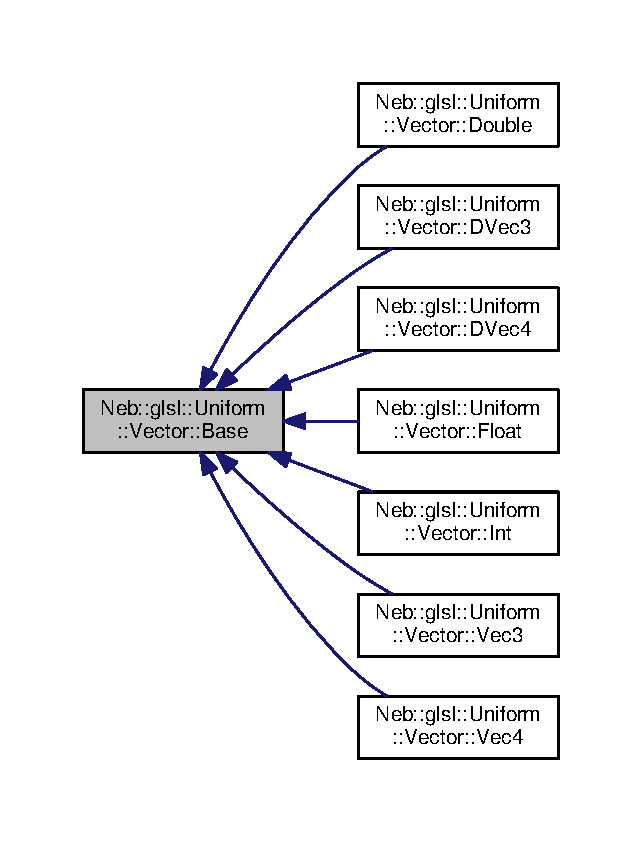
\includegraphics[width=308pt]{classNeb_1_1glsl_1_1Uniform_1_1Vector_1_1Base__inherit__graph}
\end{center}
\end{figure}
\subsection*{Public Member Functions}
\begin{DoxyCompactItemize}
\item 
\hypertarget{classNeb_1_1glsl_1_1Uniform_1_1Vector_1_1Base_af29a93d16de3f36eeb0b39f65f8a49eb}{{\bfseries Base} (std\-::string, std\-::string)}\label{classNeb_1_1glsl_1_1Uniform_1_1Vector_1_1Base_af29a93d16de3f36eeb0b39f65f8a49eb}

\item 
\hypertarget{classNeb_1_1glsl_1_1Uniform_1_1Vector_1_1Base_a957e976b781c3d895ba3714e89ae4024}{void {\bfseries locate} (std\-::shared\-\_\-ptr$<$ \hyperlink{classNeb_1_1glsl_1_1program}{program} $>$)}\label{classNeb_1_1glsl_1_1Uniform_1_1Vector_1_1Base_a957e976b781c3d895ba3714e89ae4024}

\end{DoxyCompactItemize}
\begin{Indent}{\bf Load}\par
\begin{DoxyCompactItemize}
\item 
\hypertarget{classNeb_1_1glsl_1_1Uniform_1_1Vector_1_1Base_adc3316871b991fcce743e2fd2cbc259c}{virtual void {\bfseries load} (int, physx\-::\-Px\-Vec3 const \&)}\label{classNeb_1_1glsl_1_1Uniform_1_1Vector_1_1Base_adc3316871b991fcce743e2fd2cbc259c}

\item 
\hypertarget{classNeb_1_1glsl_1_1Uniform_1_1Vector_1_1Base_abdbdbf8bbf6622c8ee70d565bede9d9c}{virtual void {\bfseries load} (int, physx\-::\-Px\-Vec4 const \&)}\label{classNeb_1_1glsl_1_1Uniform_1_1Vector_1_1Base_abdbdbf8bbf6622c8ee70d565bede9d9c}

\item 
\hypertarget{classNeb_1_1glsl_1_1Uniform_1_1Vector_1_1Base_aebb6d3b5e711315c6709ab28f6e05022}{virtual void {\bfseries load} (int, physx\-::\-Px\-Mat44 const \&)}\label{classNeb_1_1glsl_1_1Uniform_1_1Vector_1_1Base_aebb6d3b5e711315c6709ab28f6e05022}

\item 
\hypertarget{classNeb_1_1glsl_1_1Uniform_1_1Vector_1_1Base_ab5d9bdf2c08599cf4c722d8db698dcc1}{virtual void {\bfseries load} (int, int)}\label{classNeb_1_1glsl_1_1Uniform_1_1Vector_1_1Base_ab5d9bdf2c08599cf4c722d8db698dcc1}

\item 
\hypertarget{classNeb_1_1glsl_1_1Uniform_1_1Vector_1_1Base_a0500f9761ac6e639d9206dc68388a412}{virtual void {\bfseries load} (int, float $\ast$)}\label{classNeb_1_1glsl_1_1Uniform_1_1Vector_1_1Base_a0500f9761ac6e639d9206dc68388a412}

\item 
\hypertarget{classNeb_1_1glsl_1_1Uniform_1_1Vector_1_1Base_a3b602b4052959601714ef3d2aef3fd04}{virtual void {\bfseries load} (int, double $\ast$)}\label{classNeb_1_1glsl_1_1Uniform_1_1Vector_1_1Base_a3b602b4052959601714ef3d2aef3fd04}

\item 
\hypertarget{classNeb_1_1glsl_1_1Uniform_1_1Vector_1_1Base_ad2d4ca3103fefa795b0454f61c660797}{virtual void {\bfseries load} (int, float)}\label{classNeb_1_1glsl_1_1Uniform_1_1Vector_1_1Base_ad2d4ca3103fefa795b0454f61c660797}

\item 
\hypertarget{classNeb_1_1glsl_1_1Uniform_1_1Vector_1_1Base_abc57c3a333d8af08827718eef79bd83a}{virtual void {\bfseries load} (int, double)}\label{classNeb_1_1glsl_1_1Uniform_1_1Vector_1_1Base_abc57c3a333d8af08827718eef79bd83a}

\end{DoxyCompactItemize}
\end{Indent}
\subsection*{Protected Types}
\begin{DoxyCompactItemize}
\item 
enum \{ {\bfseries L\-E\-N} = 100
 \}
\end{DoxyCompactItemize}
\subsection*{Protected Attributes}
\begin{DoxyCompactItemize}
\item 
\hypertarget{classNeb_1_1glsl_1_1Uniform_1_1Vector_1_1Base_a78a4f2843f5c87f11d67b5a29c95d6c2}{std\-::string {\bfseries name1\-\_\-}}\label{classNeb_1_1glsl_1_1Uniform_1_1Vector_1_1Base_a78a4f2843f5c87f11d67b5a29c95d6c2}

\item 
\hypertarget{classNeb_1_1glsl_1_1Uniform_1_1Vector_1_1Base_a2080091cb0f43f60e48f7c667cc3d65b}{std\-::string {\bfseries name2\-\_\-}}\label{classNeb_1_1glsl_1_1Uniform_1_1Vector_1_1Base_a2080091cb0f43f60e48f7c667cc3d65b}

\item 
\hypertarget{classNeb_1_1glsl_1_1Uniform_1_1Vector_1_1Base_adada72e697489b74dcca62bd2a6404d1}{int {\bfseries c\-\_\-}}\label{classNeb_1_1glsl_1_1Uniform_1_1Vector_1_1Base_adada72e697489b74dcca62bd2a6404d1}

\item 
\hypertarget{classNeb_1_1glsl_1_1Uniform_1_1Vector_1_1Base_a3e462add25f07b5e7b2815179f928b76}{G\-Luint {\bfseries o\-\_\-} \mbox{[}L\-E\-N\mbox{]}}\label{classNeb_1_1glsl_1_1Uniform_1_1Vector_1_1Base_a3e462add25f07b5e7b2815179f928b76}

\end{DoxyCompactItemize}


\subsection{Detailed Description}
Array base class for array G\-L\-S\-L uniform 

The documentation for this class was generated from the following files\-:\begin{DoxyCompactItemize}
\item 
src/\-Nebula/\-Graphics/glsl/\-Uniform/uniform.\-hh\item 
src/\-Nebula/\-Graphics/glsl/\-Uniform/Vector.\-cc\end{DoxyCompactItemize}

\hypertarget{classNeb_1_1Scene_1_1Base}{\section{Neb\-:\-:Scene\-:\-:Base Class Reference}
\label{classNeb_1_1Scene_1_1Base}\index{Neb\-::\-Scene\-::\-Base@{Neb\-::\-Scene\-::\-Base}}
}


Inheritance diagram for Neb\-:\-:Scene\-:\-:Base\-:
\nopagebreak
\begin{figure}[H]
\begin{center}
\leavevmode
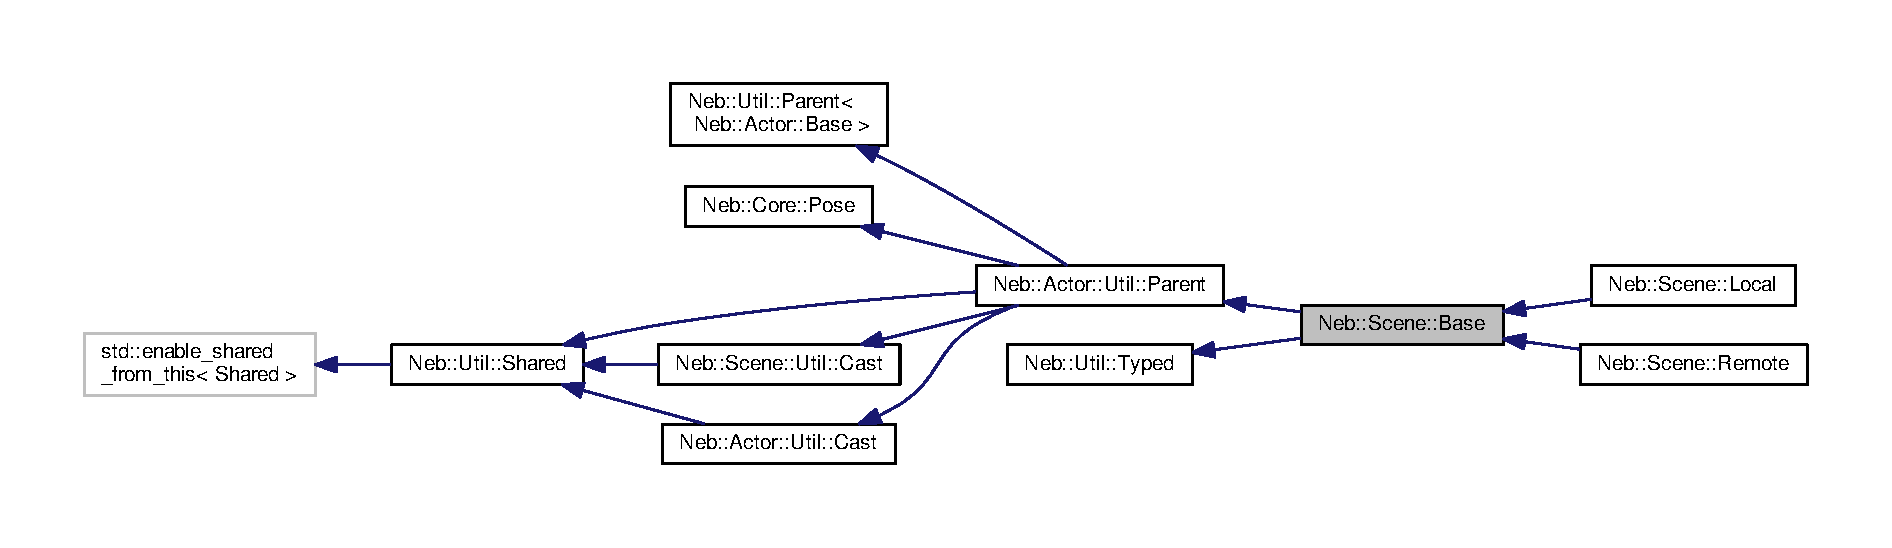
\includegraphics[width=350pt]{classNeb_1_1Scene_1_1Base__inherit__graph}
\end{center}
\end{figure}


Collaboration diagram for Neb\-:\-:Scene\-:\-:Base\-:
\nopagebreak
\begin{figure}[H]
\begin{center}
\leavevmode
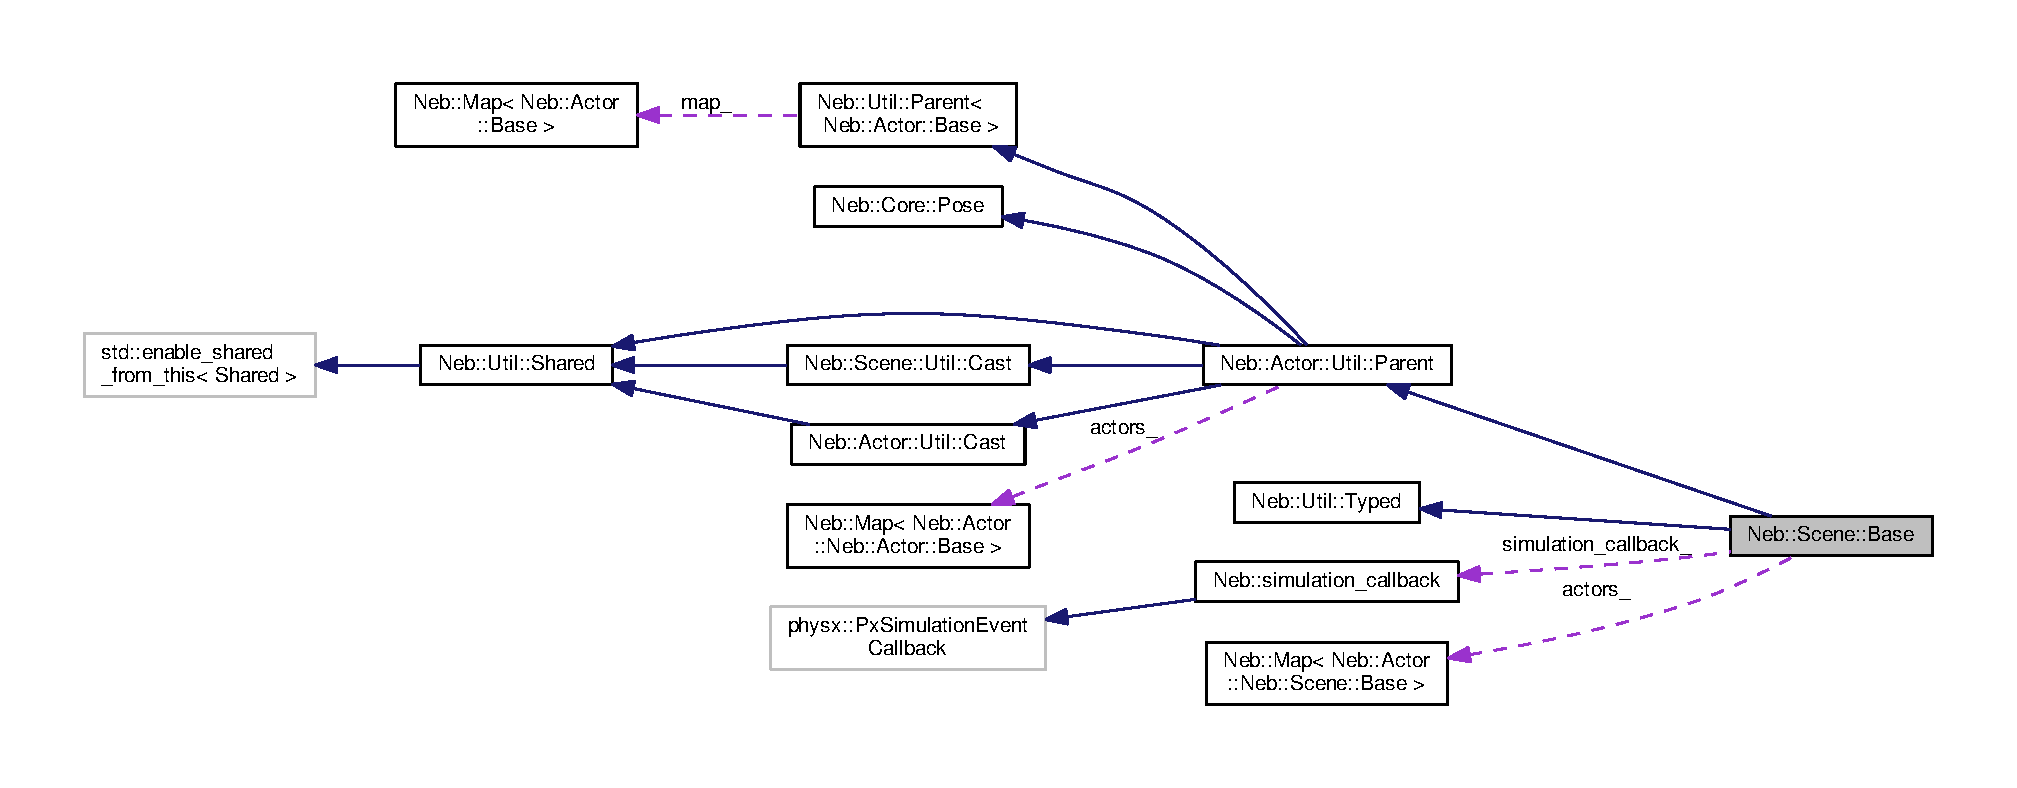
\includegraphics[width=350pt]{classNeb_1_1Scene_1_1Base__coll__graph}
\end{center}
\end{figure}
\subsection*{Public Types}
\begin{DoxyCompactItemize}
\item 
enum \{ {\bfseries N\-O\-N\-E} = 0, 
{\bfseries L\-O\-C\-A\-L}, 
{\bfseries R\-E\-M\-O\-T\-E}
 \}
\end{DoxyCompactItemize}
\subsection*{Public Member Functions}
\begin{DoxyCompactItemize}
\item 
\hypertarget{classNeb_1_1Scene_1_1Base_a3a39fc37c9dbbea3bc331341a9f64be4}{{\bfseries Base} (Neb\-::\-Scene\-::\-Util\-::\-Parent\-\_\-w)}\label{classNeb_1_1Scene_1_1Base_a3a39fc37c9dbbea3bc331341a9f64be4}

\item 
\hypertarget{classNeb_1_1Scene_1_1Base_a250ec724083495c9aa1388a21e1a2f2d}{void {\bfseries i} (int ni)}\label{classNeb_1_1Scene_1_1Base_a250ec724083495c9aa1388a21e1a2f2d}

\item 
\hypertarget{classNeb_1_1Scene_1_1Base_a6a9930917682770354731d72481de56c}{int {\bfseries i} ()}\label{classNeb_1_1Scene_1_1Base_a6a9930917682770354731d72481de56c}

\item 
\hypertarget{classNeb_1_1Scene_1_1Base_abd3b47ebbbfa21ad01fa0414ad801ebe}{void {\bfseries release} ()}\label{classNeb_1_1Scene_1_1Base_abd3b47ebbbfa21ad01fa0414ad801ebe}

\item 
\hypertarget{classNeb_1_1Scene_1_1Base_ab1a1720a07c71246df641ac388219aab}{physx\-::\-Px\-Mat44 {\bfseries get\-\_\-pose} ()}\label{classNeb_1_1Scene_1_1Base_ab1a1720a07c71246df641ac388219aab}

\item 
\hypertarget{classNeb_1_1Scene_1_1Base_af98c5a6ef603a147b4de4f6ec148ec3f}{{\footnotesize template$<$class Archive $>$ }\\void {\bfseries serialize} (Archive \&ar, unsigned int const \&version)}\label{classNeb_1_1Scene_1_1Base_af98c5a6ef603a147b4de4f6ec148ec3f}

\item 
\hypertarget{classNeb_1_1Scene_1_1Base_a876e6ed9b1f7d461f413b3530bf5c3fe}{void {\bfseries create\-\_\-physics} ()}\label{classNeb_1_1Scene_1_1Base_a876e6ed9b1f7d461f413b3530bf5c3fe}

\item 
\hypertarget{classNeb_1_1Scene_1_1Base_aa44ae1c399f8e3c38c39d76fcd687b76}{void {\bfseries fire} (Neb\-::\-Actor\-::\-Base\-\_\-w)}\label{classNeb_1_1Scene_1_1Base_aa44ae1c399f8e3c38c39d76fcd687b76}

\item 
\hypertarget{classNeb_1_1Scene_1_1Base_a63f9ef79ba12301f812ad7dd0fba8c6d}{void {\bfseries fire\-\_\-local} (Neb\-::\-Actor\-::\-Base\-\_\-w)}\label{classNeb_1_1Scene_1_1Base_a63f9ef79ba12301f812ad7dd0fba8c6d}

\item 
\hypertarget{classNeb_1_1Scene_1_1Base_ab000ef3d0fe819d74830cd1deaac9d67}{void {\bfseries fire\-\_\-remote} (Neb\-::\-Actor\-::\-Base\-\_\-w)}\label{classNeb_1_1Scene_1_1Base_ab000ef3d0fe819d74830cd1deaac9d67}

\item 
\hypertarget{classNeb_1_1Scene_1_1Base_a5525752576bf458b659eecb09be4250e}{void {\bfseries send\-\_\-actor\-\_\-update} ()}\label{classNeb_1_1Scene_1_1Base_a5525752576bf458b659eecb09be4250e}

\item 
\hypertarget{classNeb_1_1Scene_1_1Base_a508f9d9c313e3047c9bc0eaa06402620}{virtual void {\bfseries dumby} ()}\label{classNeb_1_1Scene_1_1Base_a508f9d9c313e3047c9bc0eaa06402620}

\end{DoxyCompactItemize}
\begin{Indent}{\bf Main Loop @\{}\par
\begin{DoxyCompactItemize}
\item 
\hypertarget{classNeb_1_1Scene_1_1Base_a27a040e9f1fc3b87ec6207f552d95286}{void \hyperlink{classNeb_1_1Scene_1_1Base_a27a040e9f1fc3b87ec6207f552d95286}{render} (double time, std\-::shared\-\_\-ptr$<$ \hyperlink{classNeb_1_1Camera_1_1View_1_1Base}{Neb\-::\-Camera\-::\-View\-::\-Base} $>$, std\-::shared\-\_\-ptr$<$ \hyperlink{classNeb_1_1Camera_1_1Projection_1_1Base}{Neb\-::\-Camera\-::\-Projection\-::\-Base} $>$, Neb\-::\-Graphics\-::\-Window\-::\-Base\-\_\-s)}\label{classNeb_1_1Scene_1_1Base_a27a040e9f1fc3b87ec6207f552d95286}

\begin{DoxyCompactList}\small\item\em render \end{DoxyCompactList}\item 
\hypertarget{classNeb_1_1Scene_1_1Base_aa4f3cc9f025a07f7f915a235185aaf27}{void {\bfseries draw} (Neb\-::\-Graphics\-::\-Window\-::\-Base\-\_\-s window)}\label{classNeb_1_1Scene_1_1Base_aa4f3cc9f025a07f7f915a235185aaf27}

\item 
\hypertarget{classNeb_1_1Scene_1_1Base_a9b1fbc5ffb04397abf8dc938544c5470}{void {\bfseries resize} (int w, int h)}\label{classNeb_1_1Scene_1_1Base_a9b1fbc5ffb04397abf8dc938544c5470}

\item 
\hypertarget{classNeb_1_1Scene_1_1Base_aa383aeca20d4ca9212ad5d88f82fe2e3}{void {\bfseries draw} ()}\label{classNeb_1_1Scene_1_1Base_aa383aeca20d4ca9212ad5d88f82fe2e3}

\item 
\hypertarget{classNeb_1_1Scene_1_1Base_afec6421ff59293e25f2428571cb60939}{void {\bfseries step} (double)}\label{classNeb_1_1Scene_1_1Base_afec6421ff59293e25f2428571cb60939}

\end{DoxyCompactItemize}
\end{Indent}
\begin{Indent}{\bf Accessors @\{}\par
\begin{DoxyCompactItemize}
\item 
\hypertarget{classNeb_1_1Scene_1_1Base_a9425aed0f7a62b57cc9e85838d3d8e93}{physx\-::\-Px\-Transform {\bfseries get\-Pose} ()}\label{classNeb_1_1Scene_1_1Base_a9425aed0f7a62b57cc9e85838d3d8e93}

\item 
\hypertarget{classNeb_1_1Scene_1_1Base_a9c063f947be2488466ded4657dc693e5}{physx\-::\-Px\-Transform {\bfseries get\-Pose\-Global} ()}\label{classNeb_1_1Scene_1_1Base_a9c063f947be2488466ded4657dc693e5}

\end{DoxyCompactItemize}
\end{Indent}
\subsection*{Public Attributes}
\begin{DoxyCompactItemize}
\item 
\hypertarget{classNeb_1_1Scene_1_1Base_aff1e6fae13c98a7aea6790a698dac725}{Neb\-::\-Scene\-::\-Util\-::\-Parent\-\_\-w {\bfseries parent\-\_\-}}\label{classNeb_1_1Scene_1_1Base_aff1e6fae13c98a7aea6790a698dac725}

\item 
\hypertarget{classNeb_1_1Scene_1_1Base_a9565c11540a076e5aacf5cc072a1a7eb}{int {\bfseries user\-\_\-type\-\_\-}}\label{classNeb_1_1Scene_1_1Base_a9565c11540a076e5aacf5cc072a1a7eb}

\item 
\hypertarget{classNeb_1_1Scene_1_1Base_aed874c0aa2d03387a5a126cdd0fe76e6}{physx\-::\-Px\-Simulation\-Filter\-Shader {\bfseries px\-\_\-filter\-\_\-shader\-\_\-}}\label{classNeb_1_1Scene_1_1Base_aed874c0aa2d03387a5a126cdd0fe76e6}

\item 
\hypertarget{classNeb_1_1Scene_1_1Base_a234a837620e5d08bc794ae589d1b7b3a}{\hyperlink{classNeb_1_1simulation__callback}{Neb\-::simulation\-\_\-callback} $\ast$ {\bfseries simulation\-\_\-callback\-\_\-}}\label{classNeb_1_1Scene_1_1Base_a234a837620e5d08bc794ae589d1b7b3a}

\item 
\hypertarget{classNeb_1_1Scene_1_1Base_ac1716b66b914b8fd8e04f2de16eff4b6}{physx\-::\-Px\-Scene $\ast$ {\bfseries px\-\_\-scene\-\_\-}}\label{classNeb_1_1Scene_1_1Base_ac1716b66b914b8fd8e04f2de16eff4b6}

\item 
\hypertarget{classNeb_1_1Scene_1_1Base_a9c2b45c827982c73a5601f03085095b7}{double {\bfseries last\-\_\-}}\label{classNeb_1_1Scene_1_1Base_a9c2b45c827982c73a5601f03085095b7}

\item 
\hypertarget{classNeb_1_1Scene_1_1Base_a24a4b1c10edf4b5b1656fb4764308652}{int {\bfseries i\-\_\-}}\label{classNeb_1_1Scene_1_1Base_a24a4b1c10edf4b5b1656fb4764308652}

\item 
\hypertarget{classNeb_1_1Scene_1_1Base_abd3dbc52f08bdcbb304554f595009502}{Neb\-::\-Scene\-::\-Util\-::\-Flag {\bfseries flag\-\_\-}}\label{classNeb_1_1Scene_1_1Base_abd3dbc52f08bdcbb304554f595009502}

\item 
\hypertarget{classNeb_1_1Scene_1_1Base_aba0d8709206fb88e035507117bdb2a0d}{physx\-::\-Px\-Vec3 {\bfseries gravity\-\_\-}}\label{classNeb_1_1Scene_1_1Base_aba0d8709206fb88e035507117bdb2a0d}

\item 
\hypertarget{classNeb_1_1Scene_1_1Base_ab80c1fb37a3aa9bf1c3215b0f3614214}{Neb\-::\-Scene\-::\-Util\-::\-Parent\-\_\-w {\bfseries renderable\-\_\-}}\label{classNeb_1_1Scene_1_1Base_ab80c1fb37a3aa9bf1c3215b0f3614214}

\item 
\hypertarget{classNeb_1_1Scene_1_1Base_af8f8ecef2f02a6b5b30f444a17a260ef}{\hyperlink{classNeb_1_1Map}{Neb\-::\-Map}$<$ \hyperlink{classNeb_1_1Actor_1_1Base}{Neb\-::\-Actor\-::\-Base} $>$ {\bfseries actors\-\_\-}}\label{classNeb_1_1Scene_1_1Base_af8f8ecef2f02a6b5b30f444a17a260ef}

\item 
\hypertarget{classNeb_1_1Scene_1_1Base_abea83d53821e8fee2a51afc5223e9b7c}{std\-::map$<$ std\-::string, \\*
Neb\-::\-Actor\-::\-Base\-\_\-s $>$ {\bfseries actors\-\_\-deferred\-\_\-}}\label{classNeb_1_1Scene_1_1Base_abea83d53821e8fee2a51afc5223e9b7c}

\end{DoxyCompactItemize}
\subsection*{Additional Inherited Members}


\subsection{Member Enumeration Documentation}
\hypertarget{classNeb_1_1Scene_1_1Base_ad9c45dfefe66cecc599a4707b25a95f8}{\subsubsection[{anonymous enum}]{\setlength{\rightskip}{0pt plus 5cm}anonymous enum}}\label{classNeb_1_1Scene_1_1Base_ad9c45dfefe66cecc599a4707b25a95f8}
\begin{DoxyRefDesc}{Todo}
\item[{\bf Todo}]replace types with inheritance \end{DoxyRefDesc}


The documentation for this class was generated from the following file\-:\begin{DoxyCompactItemize}
\item 
src/\-Nebula/\-Scene/Base.\-hh\end{DoxyCompactItemize}

\hypertarget{classNeb_1_1Shape_1_1Base}{\section{\-Neb\-:\-:\-Shape\-:\-:\-Base \-Class \-Reference}
\label{classNeb_1_1Shape_1_1Base}\index{\-Neb\-::\-Shape\-::\-Base@{\-Neb\-::\-Shape\-::\-Base}}
}


\-Inheritance diagram for \-Neb\-:\-:\-Shape\-:\-:\-Base\-:\nopagebreak
\begin{figure}[H]
\begin{center}
\leavevmode
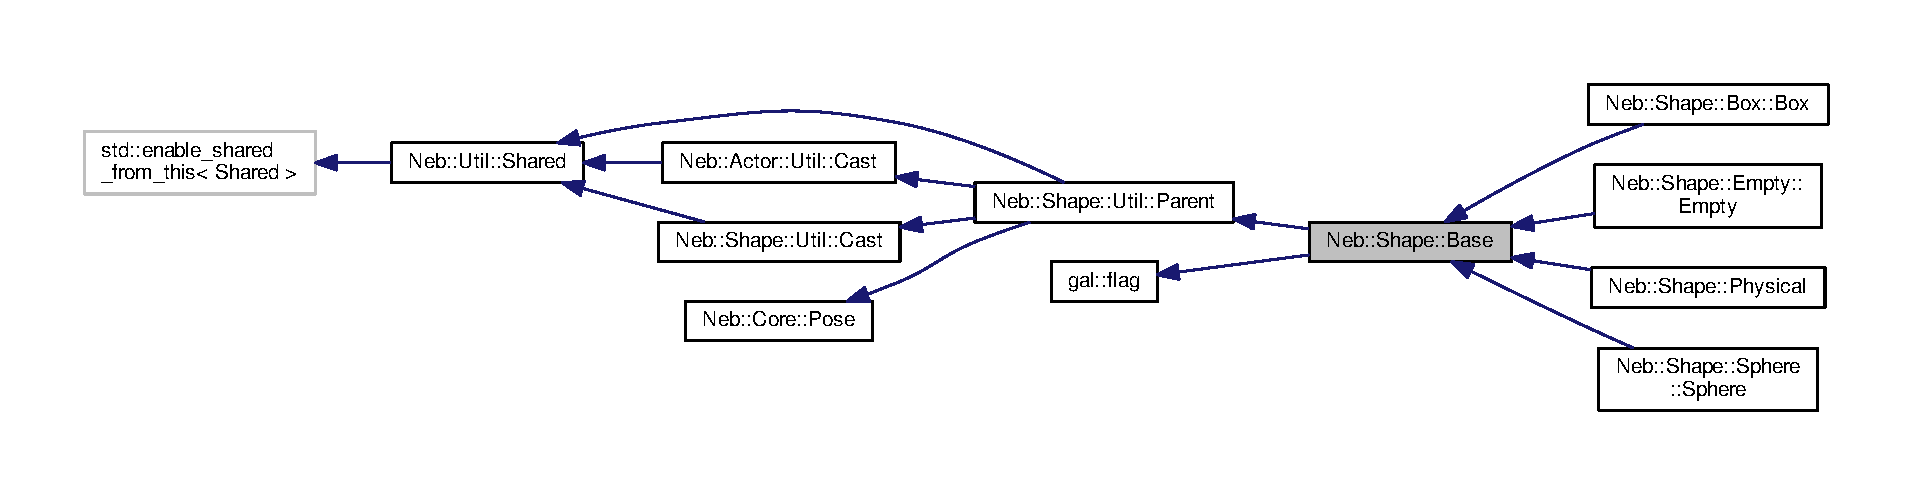
\includegraphics[width=350pt]{classNeb_1_1Shape_1_1Base__inherit__graph}
\end{center}
\end{figure}


\-Collaboration diagram for \-Neb\-:\-:\-Shape\-:\-:\-Base\-:\nopagebreak
\begin{figure}[H]
\begin{center}
\leavevmode
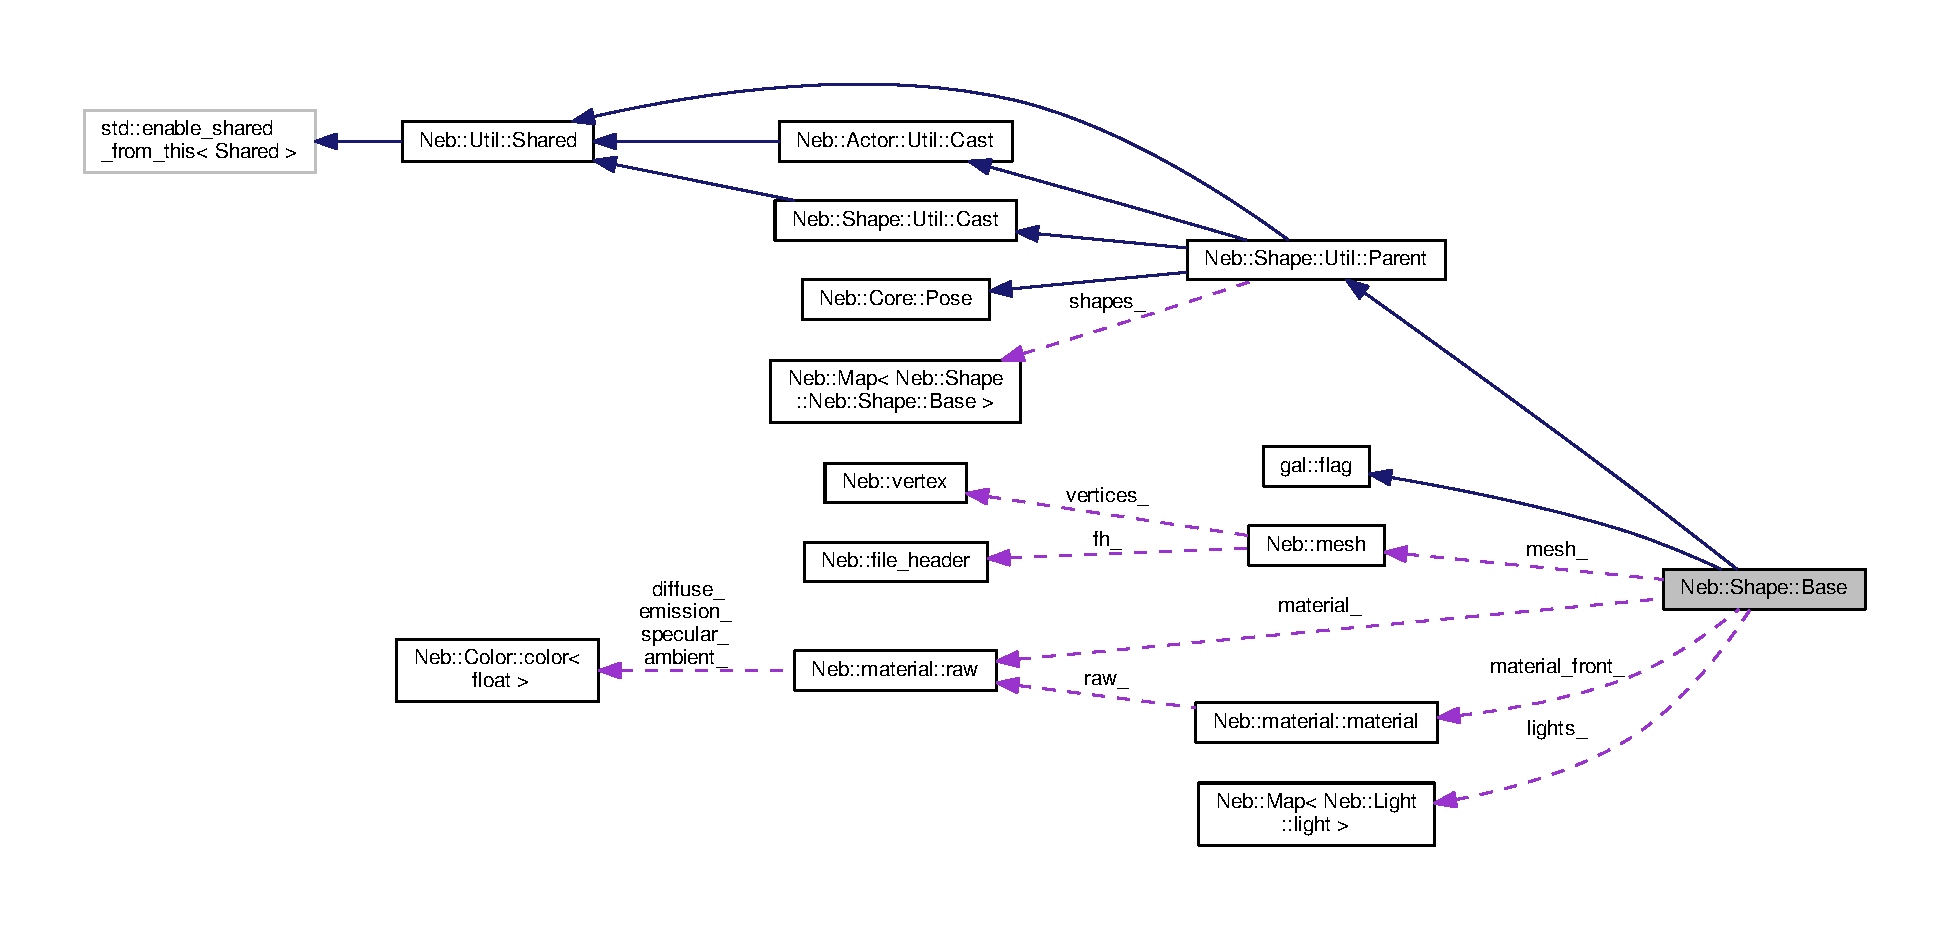
\includegraphics[width=350pt]{classNeb_1_1Shape_1_1Base__coll__graph}
\end{center}
\end{figure}
\subsection*{\-Public \-Types}
\begin{DoxyCompactItemize}
\item 
\hypertarget{classNeb_1_1Shape_1_1Base_a3b7d09a29f7f70894012e5ec8f27018e}{typedef std\-::map\*
$<$ \hyperlink{classNeb_1_1Graphics_1_1Window_1_1Base}{\-Neb\-::\-Graphics\-::\-Window\-::\-Base} \*
$\ast$, buffer\-\_\-s $>$ {\bfseries map\-\_\-t}}\label{classNeb_1_1Shape_1_1Base_a3b7d09a29f7f70894012e5ec8f27018e}

\end{DoxyCompactItemize}
\subsection*{\-Public \-Member \-Functions}
\begin{DoxyCompactItemize}
\item 
\hypertarget{classNeb_1_1Shape_1_1Base_a35afa951586265017239c2ad304a554e}{{\bfseries \-Base} (\-Neb\-::\-Shape\-::\-Util\-::\-Parent\-\_\-s parent)}\label{classNeb_1_1Shape_1_1Base_a35afa951586265017239c2ad304a554e}

\item 
\hypertarget{classNeb_1_1Shape_1_1Base_a11dd7e8eefb27d06da70638da87f0900}{void {\bfseries init} ()}\label{classNeb_1_1Shape_1_1Base_a11dd7e8eefb27d06da70638da87f0900}

\item 
\hypertarget{classNeb_1_1Shape_1_1Base_a1e46c36d898482587e96521c38bff294}{virtual void {\bfseries create\-Mesh} ()=0}\label{classNeb_1_1Shape_1_1Base_a1e46c36d898482587e96521c38bff294}

\item 
\hypertarget{classNeb_1_1Shape_1_1Base_aaa87e380e910b2bebedd62e2c04f7666}{void {\bfseries release} ()}\label{classNeb_1_1Shape_1_1Base_aaa87e380e910b2bebedd62e2c04f7666}

\item 
\hypertarget{classNeb_1_1Shape_1_1Base_afa4dd91b2963eaac1a01b59ffe4f629a}{void {\bfseries cleanup} ()}\label{classNeb_1_1Shape_1_1Base_afa4dd91b2963eaac1a01b59ffe4f629a}

\item 
\hypertarget{classNeb_1_1Shape_1_1Base_aa120c13cb2f8d462c97d6d97740df38c}{void {\bfseries step} (double const \&time, double const \&dt)}\label{classNeb_1_1Shape_1_1Base_aa120c13cb2f8d462c97d6d97740df38c}

\item 
\hypertarget{classNeb_1_1Shape_1_1Base_a30d28dc76de95cae8d78731c7ff86af8}{void {\bfseries notify\-\_\-foundation\-\_\-change\-\_\-pose} ()}\label{classNeb_1_1Shape_1_1Base_a30d28dc76de95cae8d78731c7ff86af8}

\item 
\hypertarget{classNeb_1_1Shape_1_1Base_ac7fc4a307cbc844fa931322ec26cc20e}{{\footnotesize template$<$class Archive $>$ }\\void {\bfseries serialize} (\-Archive \&ar, unsigned int const \&version)}\label{classNeb_1_1Shape_1_1Base_ac7fc4a307cbc844fa931322ec26cc20e}

\end{DoxyCompactItemize}
\begin{Indent}{\bf \-Accessors @\{}\par
\begin{DoxyCompactItemize}
\item 
\hypertarget{classNeb_1_1Shape_1_1Base_ab3d11b90943d1de0783789dc1318b670}{physx\-::\-Px\-Transform {\bfseries get\-Pose} ()}\label{classNeb_1_1Shape_1_1Base_ab3d11b90943d1de0783789dc1318b670}

\item 
\hypertarget{classNeb_1_1Shape_1_1Base_a4580b58dbab5a9a126c9b73ff253b46d}{physx\-::\-Px\-Transform {\bfseries get\-Pose\-Global} ()}\label{classNeb_1_1Shape_1_1Base_a4580b58dbab5a9a126c9b73ff253b46d}

\item 
\hypertarget{classNeb_1_1Shape_1_1Base_a1553ed6727fc83a4350919f266e84720}{\-Neb\-::\-Shape\-::\-Util\-::\-Parent\-\_\-s {\bfseries get\-Parent} ()}\label{classNeb_1_1Shape_1_1Base_a1553ed6727fc83a4350919f266e84720}

\end{DoxyCompactItemize}
\end{Indent}
\begin{Indent}{\bf \-Rendering @\{}\par
\begin{DoxyCompactItemize}
\item 
\hypertarget{classNeb_1_1Shape_1_1Base_a6ead2ae23f4a40c548557d7f4ca0776a}{void {\bfseries load\-\_\-lights} (int \&i, physx\-::\-Px\-Mat44 space)}\label{classNeb_1_1Shape_1_1Base_a6ead2ae23f4a40c548557d7f4ca0776a}

\item 
\hypertarget{classNeb_1_1Shape_1_1Base_a4af3075465d25cfc80e5d482175d36a5}{void {\bfseries draw} (\-Neb\-::\-Graphics\-::\-Window\-::\-Base\-\_\-s, physx\-::\-Px\-Mat44 space)}\label{classNeb_1_1Shape_1_1Base_a4af3075465d25cfc80e5d482175d36a5}

\item 
\hypertarget{classNeb_1_1Shape_1_1Base_acf1c451755d1c444d561140984215b2e}{void {\bfseries model\-\_\-load} (physx\-::\-Px\-Mat44 space)}\label{classNeb_1_1Shape_1_1Base_acf1c451755d1c444d561140984215b2e}

\item 
\hypertarget{classNeb_1_1Shape_1_1Base_a5447e4b4946dc45eedca9397a317a92c}{void {\bfseries init\-\_\-buffer} (\-Neb\-::\-Graphics\-::\-Window\-::\-Base\-\_\-s, std\-::shared\-\_\-ptr$<$ \hyperlink{classNeb_1_1glsl_1_1program}{\-Neb\-::glsl\-::program} $>$ p)}\label{classNeb_1_1Shape_1_1Base_a5447e4b4946dc45eedca9397a317a92c}

\item 
\hypertarget{classNeb_1_1Shape_1_1Base_a782a3f9f80564ea65dca53dfd55042e9}{virtual void {\bfseries draw\-\_\-elements} (\-Neb\-::\-Graphics\-::\-Window\-::\-Base\-\_\-s, physx\-::\-Px\-Mat44 space)}\label{classNeb_1_1Shape_1_1Base_a782a3f9f80564ea65dca53dfd55042e9}

\end{DoxyCompactItemize}
\end{Indent}
\begin{Indent}{\bf \-Index}\par
\begin{DoxyCompactItemize}
\item 
\hypertarget{classNeb_1_1Shape_1_1Base_a34ad21e9ff6525505644d5429f071a1e}{void {\bfseries i} (int ni)}\label{classNeb_1_1Shape_1_1Base_a34ad21e9ff6525505644d5429f071a1e}

\item 
\hypertarget{classNeb_1_1Shape_1_1Base_a17f8b9c1ee2fc0d5eacb034256ba409f}{int {\bfseries i} ()}\label{classNeb_1_1Shape_1_1Base_a17f8b9c1ee2fc0d5eacb034256ba409f}

\end{DoxyCompactItemize}
\end{Indent}
\subsection*{\-Public \-Attributes}
\begin{DoxyCompactItemize}
\item 
\hypertarget{classNeb_1_1Shape_1_1Base_a8df6eca6a95840d9273c96b39085c9c7}{\-Neb\-::\-Shape\-::\-Util\-::\-Flag {\bfseries flag\-\_\-}}\label{classNeb_1_1Shape_1_1Base_a8df6eca6a95840d9273c96b39085c9c7}

\item 
\hypertarget{classNeb_1_1Shape_1_1Base_a41645b682b7228a154fdc1482776cb27}{physx\-::\-Px\-Transform \hyperlink{classNeb_1_1Shape_1_1Base_a41645b682b7228a154fdc1482776cb27}{pose\-\_\-}}\label{classNeb_1_1Shape_1_1Base_a41645b682b7228a154fdc1482776cb27}

\begin{DoxyCompactList}\small\item\em \-Pose. \end{DoxyCompactList}\item 
\hypertarget{classNeb_1_1Shape_1_1Base_a42ca0cc9b1f7d1ae4cdb62ac71406d63}{physx\-::\-Px\-Vec3 \hyperlink{classNeb_1_1Shape_1_1Base_a42ca0cc9b1f7d1ae4cdb62ac71406d63}{s\-\_\-}}\label{classNeb_1_1Shape_1_1Base_a42ca0cc9b1f7d1ae4cdb62ac71406d63}

\begin{DoxyCompactList}\small\item\em \-Scale. \end{DoxyCompactList}\item 
\hypertarget{classNeb_1_1Shape_1_1Base_a7928c3c015047215fbea0cd14c1df2fb}{std\-::string \hyperlink{classNeb_1_1Shape_1_1Base_a7928c3c015047215fbea0cd14c1df2fb}{image\-\_\-}}\label{classNeb_1_1Shape_1_1Base_a7928c3c015047215fbea0cd14c1df2fb}

\begin{DoxyCompactList}\small\item\em \-Name of image file. \end{DoxyCompactList}\item 
\hypertarget{classNeb_1_1Shape_1_1Base_a15532801c8800a578073ed2869c21367}{std\-::string \hyperlink{classNeb_1_1Shape_1_1Base_a15532801c8800a578073ed2869c21367}{normal\-\_\-}}\label{classNeb_1_1Shape_1_1Base_a15532801c8800a578073ed2869c21367}

\begin{DoxyCompactList}\small\item\em \-Name of normal map file. \end{DoxyCompactList}\item 
\hypertarget{classNeb_1_1Shape_1_1Base_adc5a26798ca0d8806ff6625bf2b66741}{\hyperlink{structNeb_1_1material_1_1raw}{\-Neb\-::material\-::raw} \hyperlink{classNeb_1_1Shape_1_1Base_adc5a26798ca0d8806ff6625bf2b66741}{material\-\_\-}}\label{classNeb_1_1Shape_1_1Base_adc5a26798ca0d8806ff6625bf2b66741}

\begin{DoxyCompactList}\small\item\em \-Material. \end{DoxyCompactList}\item 
\hypertarget{classNeb_1_1Shape_1_1Base_ac080174461c07d79ba809ae1291d3260}{int \hyperlink{classNeb_1_1Shape_1_1Base_ac080174461c07d79ba809ae1291d3260}{i\-\_\-}}\label{classNeb_1_1Shape_1_1Base_ac080174461c07d79ba809ae1291d3260}

\begin{DoxyCompactList}\small\item\em \-I\-D. \end{DoxyCompactList}\item 
\hypertarget{classNeb_1_1Shape_1_1Base_a35f56410d30b2a2e343032f3455e442b}{\hyperlink{classNeb_1_1material_1_1material}{\-Neb\-::material\-::material} {\bfseries material\-\_\-front\-\_\-}}\label{classNeb_1_1Shape_1_1Base_a35f56410d30b2a2e343032f3455e442b}

\item 
\hypertarget{classNeb_1_1Shape_1_1Base_a2086d7c205e5252154638253ae866773}{\hyperlink{classNeb_1_1mesh}{mesh} {\bfseries mesh\-\_\-}}\label{classNeb_1_1Shape_1_1Base_a2086d7c205e5252154638253ae866773}

\item 
\hypertarget{classNeb_1_1Shape_1_1Base_a1b211583183a5ade3976dae341fa474b}{map\-\_\-t {\bfseries context\-\_\-}}\label{classNeb_1_1Shape_1_1Base_a1b211583183a5ade3976dae341fa474b}

\item 
\hypertarget{classNeb_1_1Shape_1_1Base_a8e2e8da14ea737c5981da827615d54c8}{\-Neb\-::program\-\_\-name\-::e {\bfseries program\-\_\-}}\label{classNeb_1_1Shape_1_1Base_a8e2e8da14ea737c5981da827615d54c8}

\item 
\hypertarget{classNeb_1_1Shape_1_1Base_a905e6814c389cbeda30725da78fa4406}{\-Neb\-::\-Shape\-::\-Util\-::\-Parent\-\_\-w \hyperlink{classNeb_1_1Shape_1_1Base_a905e6814c389cbeda30725da78fa4406}{parent\-\_\-}}\label{classNeb_1_1Shape_1_1Base_a905e6814c389cbeda30725da78fa4406}

\begin{DoxyCompactList}\small\item\em \-Parent. \end{DoxyCompactList}\end{DoxyCompactItemize}


\-The documentation for this class was generated from the following files\-:\begin{DoxyCompactItemize}
\item 
src/\-Nebula/\-Shape/\-Base.\-hh\item 
src/\-Nebula/\-Shape/\-Base.\-cc\end{DoxyCompactItemize}

\hypertarget{classNeb_1_1Graphics_1_1GUI_1_1Layout_1_1Base}{\section{Neb\-:\-:Graphics\-:\-:G\-U\-I\-:\-:Layout\-:\-:Base Class Reference}
\label{classNeb_1_1Graphics_1_1GUI_1_1Layout_1_1Base}\index{Neb\-::\-Graphics\-::\-G\-U\-I\-::\-Layout\-::\-Base@{Neb\-::\-Graphics\-::\-G\-U\-I\-::\-Layout\-::\-Base}}
}


Base  




{\ttfamily \#include $<$Base.\-hh$>$}



Collaboration diagram for Neb\-:\-:Graphics\-:\-:G\-U\-I\-:\-:Layout\-:\-:Base\-:
\nopagebreak
\begin{figure}[H]
\begin{center}
\leavevmode
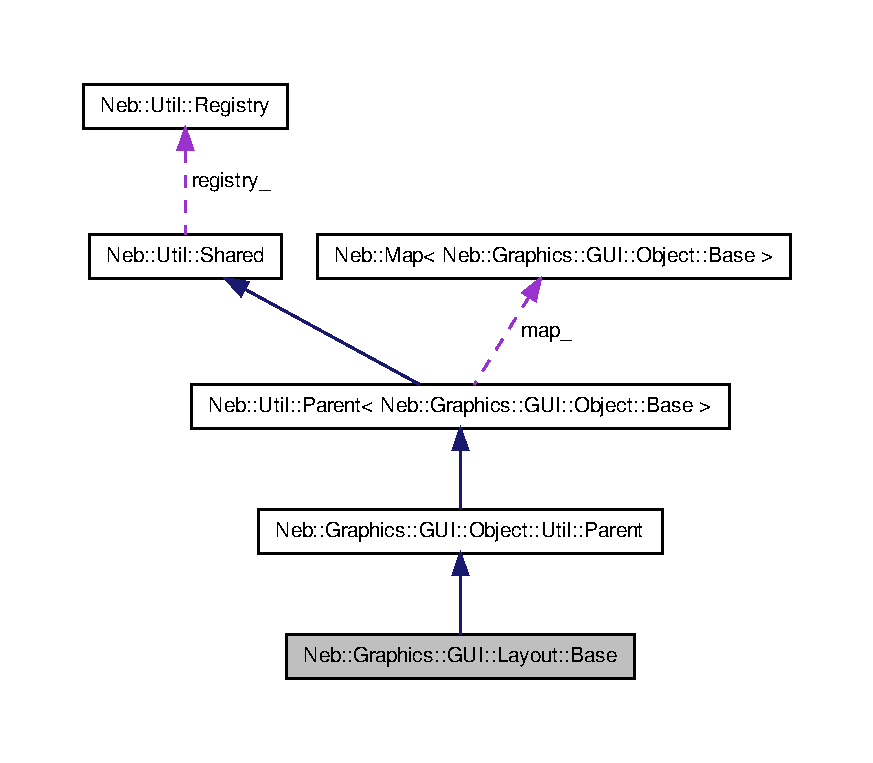
\includegraphics[width=184pt]{classNeb_1_1Graphics_1_1GUI_1_1Layout_1_1Base__coll__graph}
\end{center}
\end{figure}
\subsection*{Public Member Functions}
\begin{DoxyCompactItemize}
\item 
\hypertarget{classNeb_1_1Graphics_1_1GUI_1_1Layout_1_1Base_a1b2f473c9113eece88467beca024a215}{{\bfseries Base} (Neb\-::\-Graphics\-::\-G\-U\-I\-::\-Layout\-::\-Util\-::\-Parent\-\_\-s parent)}\label{classNeb_1_1Graphics_1_1GUI_1_1Layout_1_1Base_a1b2f473c9113eece88467beca024a215}

\item 
\hypertarget{classNeb_1_1Graphics_1_1GUI_1_1Layout_1_1Base_a7d4eefbfaf39c14f80c34a50e483e226}{virtual void {\bfseries init} ()}\label{classNeb_1_1Graphics_1_1GUI_1_1Layout_1_1Base_a7d4eefbfaf39c14f80c34a50e483e226}

\item 
\hypertarget{classNeb_1_1Graphics_1_1GUI_1_1Layout_1_1Base_af784b6ba641476e369e1665766a6f6a3}{Neb\-::\-Graphics\-::\-G\-U\-I\-::\-Layout\-::\-Util\-::\-Parent\-\_\-s {\bfseries get\-Parent} ()}\label{classNeb_1_1Graphics_1_1GUI_1_1Layout_1_1Base_af784b6ba641476e369e1665766a6f6a3}

\item 
\hypertarget{classNeb_1_1Graphics_1_1GUI_1_1Layout_1_1Base_ae427bfc003d7f02081ec340790dedba5}{void {\bfseries connect} ()}\label{classNeb_1_1Graphics_1_1GUI_1_1Layout_1_1Base_ae427bfc003d7f02081ec340790dedba5}

\item 
\hypertarget{classNeb_1_1Graphics_1_1GUI_1_1Layout_1_1Base_aa51592ea353a7921c9172bcd612047a4}{int {\bfseries search} (int button, int action, int mods)}\label{classNeb_1_1Graphics_1_1GUI_1_1Layout_1_1Base_aa51592ea353a7921c9172bcd612047a4}

\item 
\hypertarget{classNeb_1_1Graphics_1_1GUI_1_1Layout_1_1Base_a3207514a6c4b8be12165a930de390ebb}{int {\bfseries mouse\-\_\-button\-\_\-fun} (int button, int action, int mods)}\label{classNeb_1_1Graphics_1_1GUI_1_1Layout_1_1Base_a3207514a6c4b8be12165a930de390ebb}

\item 
\hypertarget{classNeb_1_1Graphics_1_1GUI_1_1Layout_1_1Base_a7da0d6f91d6db9e6d91cbd938b36d9d7}{int {\bfseries key\-\_\-fun} (int, int, int, int)}\label{classNeb_1_1Graphics_1_1GUI_1_1Layout_1_1Base_a7da0d6f91d6db9e6d91cbd938b36d9d7}

\end{DoxyCompactItemize}
{\bf }\par
\begin{DoxyCompactItemize}
\item 
\hypertarget{classNeb_1_1Graphics_1_1GUI_1_1Layout_1_1Base_a0888582e9cdc248839bd4c5d3dae57f7}{void \hyperlink{classNeb_1_1Graphics_1_1GUI_1_1Layout_1_1Base_a0888582e9cdc248839bd4c5d3dae57f7}{render} (double time)}\label{classNeb_1_1Graphics_1_1GUI_1_1Layout_1_1Base_a0888582e9cdc248839bd4c5d3dae57f7}

\begin{DoxyCompactList}\small\item\em Main Loop. \end{DoxyCompactList}\item 
\hypertarget{classNeb_1_1Graphics_1_1GUI_1_1Layout_1_1Base_acea4b693686386a7eba8cc859e7fce7a}{void {\bfseries draw} ()}\label{classNeb_1_1Graphics_1_1GUI_1_1Layout_1_1Base_acea4b693686386a7eba8cc859e7fce7a}

\end{DoxyCompactItemize}

\subsection*{Public Attributes}
\begin{DoxyCompactItemize}
\item 
\hypertarget{classNeb_1_1Graphics_1_1GUI_1_1Layout_1_1Base_a28c47c2cddf86a88653b13d47fa1a543}{physx\-::\-Px\-Mat44 {\bfseries ortho\-\_\-}}\label{classNeb_1_1Graphics_1_1GUI_1_1Layout_1_1Base_a28c47c2cddf86a88653b13d47fa1a543}

\item 
\hypertarget{classNeb_1_1Graphics_1_1GUI_1_1Layout_1_1Base_a924d8e0e498904df1d119f6625fba4c2}{\hyperlink{classNeb_1_1Map}{Neb\-::\-Map}\\*
$<$ \hyperlink{classNeb_1_1gui_1_1object_1_1object}{Neb\-::gui\-::object\-::object} $>$ {\bfseries objects\-\_\-}}\label{classNeb_1_1Graphics_1_1GUI_1_1Layout_1_1Base_a924d8e0e498904df1d119f6625fba4c2}

\item 
\hypertarget{classNeb_1_1Graphics_1_1GUI_1_1Layout_1_1Base_a1ef732e458fa71c15ed952c0b87a122b}{Neb\-::\-Graphics\-::\-G\-U\-I\-::\-Layout\-::\-Util\-::\-Parent\-\_\-w {\bfseries parent\-\_\-}}\label{classNeb_1_1Graphics_1_1GUI_1_1Layout_1_1Base_a1ef732e458fa71c15ed952c0b87a122b}

\item 
\hypertarget{classNeb_1_1Graphics_1_1GUI_1_1Layout_1_1Base_a0546cceee20db9ace4701e8c3dcc1602}{\begin{tabbing}
xx\=xx\=xx\=xx\=xx\=xx\=xx\=xx\=xx\=\kill
struct \{\\
\hypertarget{structNeb_1_1Graphics_1_1GUI_1_1Layout_1_1Base_1_1@4_a66d569bc79d874c757dd9dbe4c3c290d}{\>boost::signals2::connection {\bfseries mouse\_button\_fun\_}\\
\hypertarget{structNeb_1_1Graphics_1_1GUI_1_1Layout_1_1Base_1_1@4_a8bb2b88e7b538a84c97bdba32f1b888d}{\>boost::signals2::connection {\bfseries key\_fun\_}\\
\} {\bfseries conns\_}}\label{classNeb_1_1Graphics_1_1GUI_1_1Layout_1_1Base_a0546cceee20db9ace4701e8c3dcc1602}
\\

\end{tabbing}\end{DoxyCompactItemize}


\subsection{Detailed Description}
Base 

The documentation for this class was generated from the following file\-:\begin{DoxyCompactItemize}
\item 
src/\-Nebula/\-Graphics/\-G\-U\-I/\-Layout/Base.\-hh\end{DoxyCompactItemize}

\hypertarget{classNeb_1_1Shape_1_1Event_1_1Base}{\section{Neb\-:\-:Shape\-:\-:Event\-:\-:Base Class Reference}
\label{classNeb_1_1Shape_1_1Event_1_1Base}\index{Neb\-::\-Shape\-::\-Event\-::\-Base@{Neb\-::\-Shape\-::\-Event\-::\-Base}}
}


The documentation for this class was generated from the following file\-:\begin{DoxyCompactItemize}
\item 
src/\-Nebula/\-Shape/\-Util/Event.\-hh\end{DoxyCompactItemize}

\hypertarget{classNeb_1_1Timer_1_1Actor_1_1Base}{\section{Neb\-:\-:Timer\-:\-:Actor\-:\-:Base Class Reference}
\label{classNeb_1_1Timer_1_1Actor_1_1Base}\index{Neb\-::\-Timer\-::\-Actor\-::\-Base@{Neb\-::\-Timer\-::\-Actor\-::\-Base}}
}
\subsection*{Public Member Functions}
\begin{DoxyCompactItemize}
\item 
\hypertarget{classNeb_1_1Timer_1_1Actor_1_1Base_abf4fc9cbf5d86bd2c36da3a9d10f262d}{{\bfseries Base} (boost\-::asio\-::io\-\_\-service \&io, boost\-::shared\-\_\-ptr$<$ \hyperlink{classNeb_1_1Actor_1_1Base}{Neb\-::\-Actor\-::\-Base} $>$, double)}\label{classNeb_1_1Timer_1_1Actor_1_1Base_abf4fc9cbf5d86bd2c36da3a9d10f262d}

\item 
\hypertarget{classNeb_1_1Timer_1_1Actor_1_1Base_a8e1f81941a3720f925aa376ef2c260e0}{virtual void {\bfseries do\-Something} ()=0}\label{classNeb_1_1Timer_1_1Actor_1_1Base_a8e1f81941a3720f925aa376ef2c260e0}

\item 
\hypertarget{classNeb_1_1Timer_1_1Actor_1_1Base_a698df59a0dc7ebb6a8f0a0dfc45f2004}{void {\bfseries activate} ()}\label{classNeb_1_1Timer_1_1Actor_1_1Base_a698df59a0dc7ebb6a8f0a0dfc45f2004}

\end{DoxyCompactItemize}
\subsection*{Public Attributes}
\begin{DoxyCompactItemize}
\item 
\hypertarget{classNeb_1_1Timer_1_1Actor_1_1Base_a901f924d54f4d8c44244586a270df37e}{boost\-::asio\-::deadline\-\_\-timer {\bfseries timer\-\_\-}}\label{classNeb_1_1Timer_1_1Actor_1_1Base_a901f924d54f4d8c44244586a270df37e}

\item 
\hypertarget{classNeb_1_1Timer_1_1Actor_1_1Base_a365e4320c4de0c27fc7518a4e1e09f8e}{boost\-::weak\-\_\-ptr$<$ \hyperlink{classNeb_1_1Actor_1_1Base}{Neb\-::\-Actor\-::\-Base} $>$ {\bfseries actor\-\_\-}}\label{classNeb_1_1Timer_1_1Actor_1_1Base_a365e4320c4de0c27fc7518a4e1e09f8e}

\end{DoxyCompactItemize}


The documentation for this class was generated from the following file\-:\begin{DoxyCompactItemize}
\item 
src/\-Nebula/timer/\-Actor/Base.\-hpp\end{DoxyCompactItemize}

\hypertarget{classNeb_1_1Actor_1_1Base}{\section{\-Neb\-:\-:\-Actor\-:\-:\-Base \-Class \-Reference}
\label{classNeb_1_1Actor_1_1Base}\index{\-Neb\-::\-Actor\-::\-Base@{\-Neb\-::\-Actor\-::\-Base}}
}


\-Base  




{\ttfamily \#include $<$\-Base.\-hh$>$}



\-Inheritance diagram for \-Neb\-:\-:\-Actor\-:\-:\-Base\-:\nopagebreak
\begin{figure}[H]
\begin{center}
\leavevmode
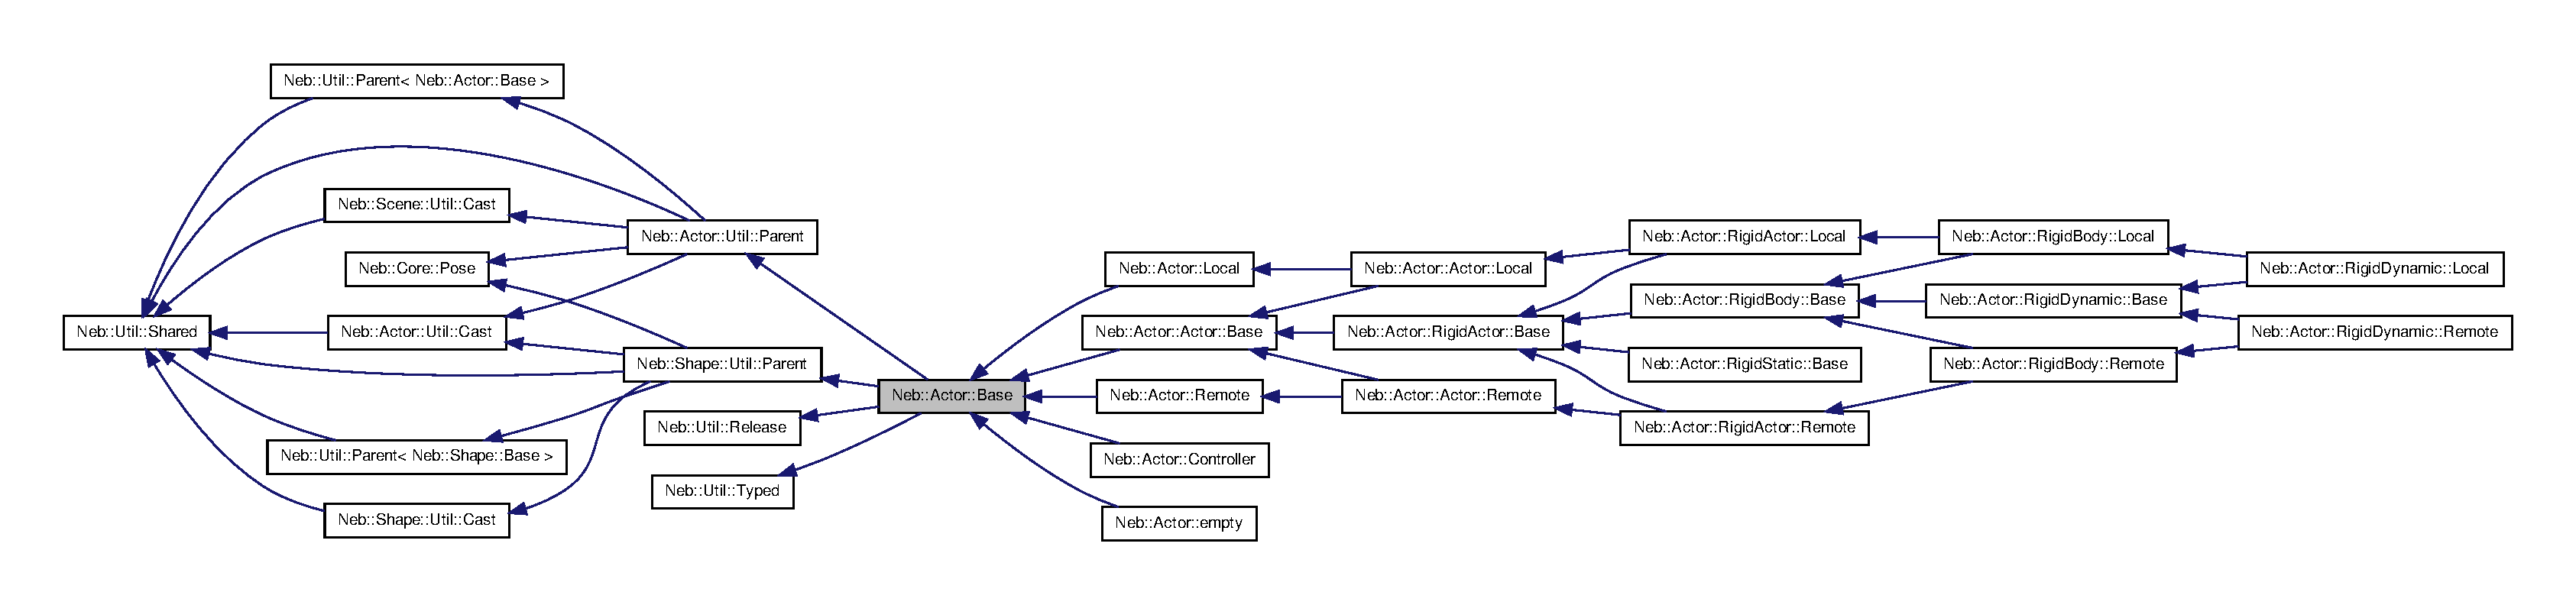
\includegraphics[width=350pt]{classNeb_1_1Actor_1_1Base__inherit__graph}
\end{center}
\end{figure}


\-Collaboration diagram for \-Neb\-:\-:\-Actor\-:\-:\-Base\-:\nopagebreak
\begin{figure}[H]
\begin{center}
\leavevmode
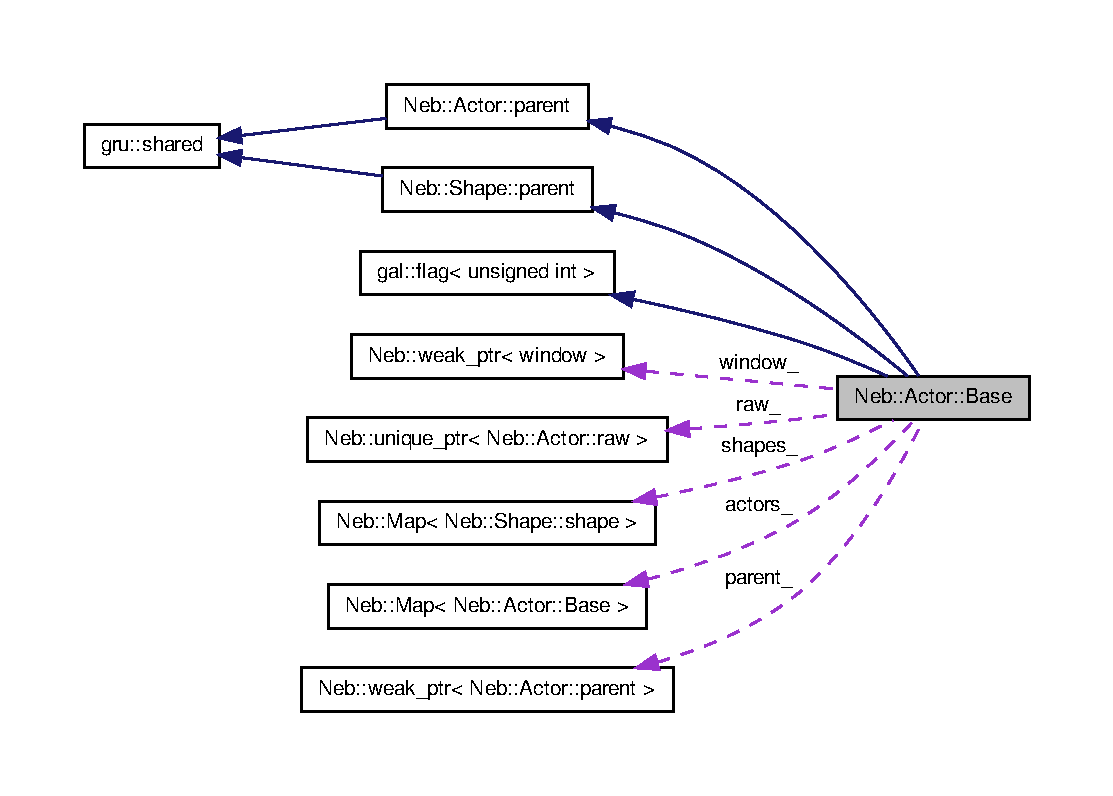
\includegraphics[width=350pt]{classNeb_1_1Actor_1_1Base__coll__graph}
\end{center}
\end{figure}
\subsection*{\-Public \-Member \-Functions}
\begin{DoxyCompactItemize}
\item 
\hypertarget{classNeb_1_1Actor_1_1Base_a2148b7903d9aebf73bcb333240e8a5ac}{{\bfseries \-Base} (\-Neb\-::\-Actor\-::\-Util\-::\-Parent\-\_\-s)}\label{classNeb_1_1Actor_1_1Base_a2148b7903d9aebf73bcb333240e8a5ac}

\item 
\hypertarget{classNeb_1_1Actor_1_1Base_ad6c67af83640455001015816eedbfc0c}{{\footnotesize template$<$class D , typename... \-Args$>$ }\\void {\bfseries dispatch} (\-Args...\-a)}\label{classNeb_1_1Actor_1_1Base_ad6c67af83640455001015816eedbfc0c}

\item 
\hypertarget{classNeb_1_1Actor_1_1Base_aea161083c16227392cc4556928f5479e}{virtual void {\bfseries init} ()}\label{classNeb_1_1Actor_1_1Base_aea161083c16227392cc4556928f5479e}

\item 
\hypertarget{classNeb_1_1Actor_1_1Base_a6fcf7946643de0bdda7ef31b089ecd7a}{virtual void {\bfseries release\-Derived} ()}\label{classNeb_1_1Actor_1_1Base_a6fcf7946643de0bdda7ef31b089ecd7a}

\item 
\hypertarget{classNeb_1_1Actor_1_1Base_a4db2db31645b73484865f665e7b181e5}{virtual void {\bfseries cleanup} ()}\label{classNeb_1_1Actor_1_1Base_a4db2db31645b73484865f665e7b181e5}

\item 
\hypertarget{classNeb_1_1Actor_1_1Base_a19d7b3eeac560db781b8dd9d7a044bef}{virtual void {\bfseries release} ()}\label{classNeb_1_1Actor_1_1Base_a19d7b3eeac560db781b8dd9d7a044bef}

\item 
\hypertarget{classNeb_1_1Actor_1_1Base_a732e42c211856137d5fa55d041606805}{void {\bfseries i} (int ni)}\label{classNeb_1_1Actor_1_1Base_a732e42c211856137d5fa55d041606805}

\item 
\hypertarget{classNeb_1_1Actor_1_1Base_a8b8facad0502a876dec354116069fc00}{int {\bfseries i} () const }\label{classNeb_1_1Actor_1_1Base_a8b8facad0502a876dec354116069fc00}

\item 
\hypertarget{classNeb_1_1Actor_1_1Base_ab093290863fcedd9ef36828de4438401}{unsigned int {\bfseries f} () const }\label{classNeb_1_1Actor_1_1Base_ab093290863fcedd9ef36828de4438401}

\item 
\hypertarget{classNeb_1_1Actor_1_1Base_a400c04ba14166e7e399630c576f626eb}{void {\bfseries f} (unsigned int flag)}\label{classNeb_1_1Actor_1_1Base_a400c04ba14166e7e399630c576f626eb}

\item 
\hypertarget{classNeb_1_1Actor_1_1Base_ae5649ec4e6bae0235f5056f8ef877f6e}{virtual void {\bfseries create\-\_\-physics} ()=0}\label{classNeb_1_1Actor_1_1Base_ae5649ec4e6bae0235f5056f8ef877f6e}

\item 
\hypertarget{classNeb_1_1Actor_1_1Base_a84a52d4a51117c510336bcad075f63d1}{virtual void {\bfseries init\-\_\-physics} ()=0}\label{classNeb_1_1Actor_1_1Base_a84a52d4a51117c510336bcad075f63d1}

\item 
\hypertarget{classNeb_1_1Actor_1_1Base_a5b5263db439a6cc2614268dd9058d302}{void {\bfseries notify\-\_\-foundation\-\_\-change\-\_\-pose} ()}\label{classNeb_1_1Actor_1_1Base_a5b5263db439a6cc2614268dd9058d302}

\item 
\hypertarget{classNeb_1_1Actor_1_1Base_a1952504069949fa29f53137cfe762274}{void {\bfseries load\-\_\-lights} (int \&, physx\-::\-Px\-Mat44)}\label{classNeb_1_1Actor_1_1Base_a1952504069949fa29f53137cfe762274}

\item 
virtual void \hyperlink{classNeb_1_1Actor_1_1Base_afc072654755bb4db2e1af77a55e7f8dd}{hit} ()
\item 
\hypertarget{classNeb_1_1Actor_1_1Base_aa8065352d9f093036db30ea7a4e04828}{virtual void {\bfseries damage} (float)}\label{classNeb_1_1Actor_1_1Base_aa8065352d9f093036db30ea7a4e04828}

\item 
\hypertarget{classNeb_1_1Actor_1_1Base_a9baf846b3bc20d710597cfa8245b4b3c}{void {\bfseries connect} (\-Neb\-::\-Graphics\-::\-Window\-::\-Base\-\_\-s)}\label{classNeb_1_1Actor_1_1Base_a9baf846b3bc20d710597cfa8245b4b3c}

\item 
\hypertarget{classNeb_1_1Actor_1_1Base_a02cc601e428cea2f36c5b8f58bf31749}{int {\bfseries key\-\_\-fun} (int, int, int, int)}\label{classNeb_1_1Actor_1_1Base_a02cc601e428cea2f36c5b8f58bf31749}

\item 
\hypertarget{classNeb_1_1Actor_1_1Base_aa7001c8845e41342c9b01a190c6026a1}{virtual int {\bfseries fire} ()}\label{classNeb_1_1Actor_1_1Base_aa7001c8845e41342c9b01a190c6026a1}

\item 
{\footnotesize template$<$class Archive $>$ }\\void \hyperlink{classNeb_1_1Actor_1_1Base_a1b1e7cf679c2cb84e532deed6a2ec90c}{serialize} (\-Archive \&ar, unsigned int const \&version)
\begin{DoxyCompactList}\small\item\em \-Serialize \end{DoxyCompactList}\item 
\hypertarget{classNeb_1_1Actor_1_1Base_a910522bc6cc99e63fda53c9c46555204}{virtual void {\bfseries serialize\-Data} (boost\-::archive\-::polymorphic\-\_\-oarchive \&ar, unsigned int const \&version)}\label{classNeb_1_1Actor_1_1Base_a910522bc6cc99e63fda53c9c46555204}

\item 
\hypertarget{classNeb_1_1Actor_1_1Base_aea6b73147535dde24fa95ec2f82c759f}{virtual void {\bfseries serialize\-Data} (boost\-::archive\-::polymorphic\-\_\-iarchive \&ar, unsigned int const \&version)}\label{classNeb_1_1Actor_1_1Base_aea6b73147535dde24fa95ec2f82c759f}

\item 
\hypertarget{classNeb_1_1Actor_1_1Base_aa4edb51f746f8d68d9fe39898e93d6e9}{void \hyperlink{classNeb_1_1Actor_1_1Base_aa4edb51f746f8d68d9fe39898e93d6e9}{save\-Update} (boost\-::archive\-::polymorphic\-\_\-oarchive \&ar, unsigned int const \&version)}\label{classNeb_1_1Actor_1_1Base_aa4edb51f746f8d68d9fe39898e93d6e9}

\begin{DoxyCompactList}\small\item\em \-Serialize specialization \end{DoxyCompactList}\item 
\hypertarget{classNeb_1_1Actor_1_1Base_a188f918586281aa28c3cc31044614aba}{void \hyperlink{classNeb_1_1Actor_1_1Base_a188f918586281aa28c3cc31044614aba}{load\-Update} (boost\-::archive\-::polymorphic\-\_\-iarchive \&ar, unsigned int const \&version)}\label{classNeb_1_1Actor_1_1Base_a188f918586281aa28c3cc31044614aba}

\begin{DoxyCompactList}\small\item\em \-Serialize specialization \end{DoxyCompactList}\end{DoxyCompactItemize}
\begin{Indent}{\bf \-Stepping @\{}\par
\begin{DoxyCompactItemize}
\item 
\hypertarget{classNeb_1_1Actor_1_1Base_ae06b2570b603d98996e8c629c946962b}{virtual void {\bfseries step} (double const \&time, double const \&dt)}\label{classNeb_1_1Actor_1_1Base_ae06b2570b603d98996e8c629c946962b}

\end{DoxyCompactItemize}
\end{Indent}
\begin{Indent}{\bf \-Render @\{}\par
\begin{DoxyCompactItemize}
\item 
\hypertarget{classNeb_1_1Actor_1_1Base_aa7a1124c6d32fb41ecf26f2d7c2a486a}{void {\bfseries draw} (\-Neb\-::\-Graphics\-::\-Window\-::\-Base\-\_\-s, physx\-::\-Px\-Transform)}\label{classNeb_1_1Actor_1_1Base_aa7a1124c6d32fb41ecf26f2d7c2a486a}

\end{DoxyCompactItemize}
\end{Indent}
\begin{Indent}{\bf \-Accessors @\{}\par
\begin{DoxyCompactItemize}
\item 
\hypertarget{classNeb_1_1Actor_1_1Base_a3125fb49728707613266d4818df328cf}{\hyperlink{classNeb_1_1Actor_1_1Util_1_1Address}{\-Neb\-::\-Actor\-::\-Util\-::\-Address} {\bfseries get\-Address} () const }\label{classNeb_1_1Actor_1_1Base_a3125fb49728707613266d4818df328cf}

\item 
\hypertarget{classNeb_1_1Actor_1_1Base_aac89b4475a9443894c9814472702adcb}{virtual physx\-::\-Px\-Transform {\bfseries get\-Pose} ()}\label{classNeb_1_1Actor_1_1Base_aac89b4475a9443894c9814472702adcb}

\item 
\hypertarget{classNeb_1_1Actor_1_1Base_a76f34261b14ea648f42da355138efc9b}{virtual physx\-::\-Px\-Transform {\bfseries get\-Pose\-Global} ()}\label{classNeb_1_1Actor_1_1Base_a76f34261b14ea648f42da355138efc9b}

\item 
\hypertarget{classNeb_1_1Actor_1_1Base_a37766d7d2d3a32a90e4a81d039248588}{\-Neb\-::\-Actor\-::\-Util\-::\-Parent\-\_\-s {\bfseries get\-Parent} ()}\label{classNeb_1_1Actor_1_1Base_a37766d7d2d3a32a90e4a81d039248588}

\item 
\hypertarget{classNeb_1_1Actor_1_1Base_a98dd3ef316b4d28c5f36efa2d1e73966}{void {\bfseries set\-Pose} (physx\-::\-Px\-Transform pose)}\label{classNeb_1_1Actor_1_1Base_a98dd3ef316b4d28c5f36efa2d1e73966}

\end{DoxyCompactItemize}
\end{Indent}
\subsection*{\-Public \-Attributes}
\begin{DoxyCompactItemize}
\item 
\-Neb\-::\-Actor\-::mode\-\_\-update\-::e \hyperlink{classNeb_1_1Actor_1_1Base_ad51160f955b8bff638c938360ff3ce00}{mode\-\_\-update\-\_\-}
\item 
\hypertarget{classNeb_1_1Actor_1_1Base_af67fc9f70e192a9035e572cc95f5d820}{\begin{tabbing}
xx\=xx\=xx\=xx\=xx\=xx\=xx\=xx\=xx\=\kill
struct \{\\
\>boost::signals2::connection {\bfseries key\_fun\_}\\
\} {\bfseries conn\_}}\label{classNeb_1_1Actor_1_1Base_af67fc9f70e192a9035e572cc95f5d820}
\\

\end{tabbing}\item 
\hypertarget{classNeb_1_1Actor_1_1Base_a1e076d29556f0c72028812137bcce036}{\-Neb\-::\-Actor\-::mode\-\_\-create\-::e {\bfseries mode\-\_\-create\-\_\-}}\label{classNeb_1_1Actor_1_1Base_a1e076d29556f0c72028812137bcce036}

\item 
\hypertarget{classNeb_1_1Actor_1_1Base_a22cd602ab66488cd6083eda09d048128}{\-Neb\-::\-Actor\-::\-Util\-::\-Flag {\bfseries flag\-\_\-}}\label{classNeb_1_1Actor_1_1Base_a22cd602ab66488cd6083eda09d048128}

\item 
\hypertarget{classNeb_1_1Actor_1_1Base_aa75915d9b4f44a657a85033f5b81f75d}{std\-::string {\bfseries name\-\_\-}}\label{classNeb_1_1Actor_1_1Base_aa75915d9b4f44a657a85033f5b81f75d}

\item 
\hypertarget{classNeb_1_1Actor_1_1Base_aacd62145604cea516d4f1d8e25d548be}{physx\-::\-Px\-Transform {\bfseries pose\-\_\-}}\label{classNeb_1_1Actor_1_1Base_aacd62145604cea516d4f1d8e25d548be}

\item 
\hypertarget{classNeb_1_1Actor_1_1Base_aee5edd3b6023075d864409d97d0a2d08}{physx\-::\-Px\-Vec3 \hyperlink{classNeb_1_1Actor_1_1Base_aee5edd3b6023075d864409d97d0a2d08}{n\-\_\-}}\label{classNeb_1_1Actor_1_1Base_aee5edd3b6023075d864409d97d0a2d08}

\begin{DoxyCompactList}\small\item\em \-Normal for planes. \end{DoxyCompactList}\item 
\hypertarget{classNeb_1_1Actor_1_1Base_a2997b3c2a550037b6b7cefd17ad91df1}{float \hyperlink{classNeb_1_1Actor_1_1Base_a2997b3c2a550037b6b7cefd17ad91df1}{d\-\_\-}}\label{classNeb_1_1Actor_1_1Base_a2997b3c2a550037b6b7cefd17ad91df1}

\begin{DoxyCompactList}\small\item\em \-Distance for planes. \end{DoxyCompactList}\item 
\hypertarget{classNeb_1_1Actor_1_1Base_a43300c3cb97e26f377c6059c892c047f}{physx\-::\-Px\-Vec3 {\bfseries velocity\-\_\-}}\label{classNeb_1_1Actor_1_1Base_a43300c3cb97e26f377c6059c892c047f}

\item 
\hypertarget{classNeb_1_1Actor_1_1Base_aa02c9782ff85fe0093ba5c49b84fd606}{float {\bfseries density\-\_\-}}\label{classNeb_1_1Actor_1_1Base_aa02c9782ff85fe0093ba5c49b84fd606}

\item 
\hypertarget{classNeb_1_1Actor_1_1Base_a1e6023de96fd6010c8654b793eb9602b}{\hyperlink{classNeb_1_1Filter_1_1Data}{\-Neb\-::\-Filter\-::\-Data} {\bfseries simulation\-\_\-}}\label{classNeb_1_1Actor_1_1Base_a1e6023de96fd6010c8654b793eb9602b}

\item 
\hypertarget{classNeb_1_1Actor_1_1Base_a80c205ec3b27adb6abacad3a01c0d593}{\hyperlink{classNeb_1_1Filter_1_1Data}{\-Neb\-::\-Filter\-::\-Data} {\bfseries scene\-\_\-query\-\_\-}}\label{classNeb_1_1Actor_1_1Base_a80c205ec3b27adb6abacad3a01c0d593}

\item 
\hypertarget{classNeb_1_1Actor_1_1Base_a5d433af5f8b9814e8b9255992d4a1176}{double {\bfseries health\-\_\-}}\label{classNeb_1_1Actor_1_1Base_a5d433af5f8b9814e8b9255992d4a1176}

\item 
\hypertarget{classNeb_1_1Actor_1_1Base_a037d85da810e1cc39361ea1f25ff7df7}{int \hyperlink{classNeb_1_1Actor_1_1Base_a037d85da810e1cc39361ea1f25ff7df7}{i\-\_\-}}\label{classNeb_1_1Actor_1_1Base_a037d85da810e1cc39361ea1f25ff7df7}

\begin{DoxyCompactList}\small\item\em \-I\-D. \end{DoxyCompactList}\item 
\hypertarget{classNeb_1_1Actor_1_1Base_a3d8c3b2ccad9d8322be09fdc161dca9a}{\-Neb\-::\-Actor\-::\-Util\-::\-Parent\-\_\-s \hyperlink{classNeb_1_1Actor_1_1Base_a3d8c3b2ccad9d8322be09fdc161dca9a}{parent\-\_\-}}\label{classNeb_1_1Actor_1_1Base_a3d8c3b2ccad9d8322be09fdc161dca9a}

\begin{DoxyCompactList}\small\item\em \-Parent. \end{DoxyCompactList}\end{DoxyCompactItemize}
\subsection*{\-Private \-Member \-Functions}
\begin{DoxyCompactItemize}
\item 
virtual \-Neb\-::\-Actor\-::\-Base\-\_\-s \hyperlink{classNeb_1_1Actor_1_1Base_ab919ee115817b522dffff38aa58d670c}{insert\-Actor} (\-Neb\-::\-Actor\-::\-Base\-\_\-s actor)
\end{DoxyCompactItemize}


\subsection{\-Detailed \-Description}
\-Base 

\subsection{\-Member \-Function \-Documentation}
\hypertarget{classNeb_1_1Actor_1_1Base_afc072654755bb4db2e1af77a55e7f8dd}{\index{\-Neb\-::\-Actor\-::\-Base@{\-Neb\-::\-Actor\-::\-Base}!hit@{hit}}
\index{hit@{hit}!Neb::Actor::Base@{\-Neb\-::\-Actor\-::\-Base}}
\subsubsection[{hit}]{\setlength{\rightskip}{0pt plus 5cm}void {\bf \-Neb\-::\-Actor\-::\-Base\-::hit} (
\begin{DoxyParamCaption}
{}
\end{DoxyParamCaption}
)\hspace{0.3cm}{\ttfamily  \mbox{[}virtual\mbox{]}}}}\label{classNeb_1_1Actor_1_1Base_afc072654755bb4db2e1af77a55e7f8dd}
\begin{DoxyRefDesc}{\-Todo}
\item[\hyperlink{todo__todo000001}{\-Todo}]move to derived class \end{DoxyRefDesc}
\hypertarget{classNeb_1_1Actor_1_1Base_ab919ee115817b522dffff38aa58d670c}{\index{\-Neb\-::\-Actor\-::\-Base@{\-Neb\-::\-Actor\-::\-Base}!insert\-Actor@{insert\-Actor}}
\index{insert\-Actor@{insert\-Actor}!Neb::Actor::Base@{\-Neb\-::\-Actor\-::\-Base}}
\subsubsection[{insert\-Actor}]{\setlength{\rightskip}{0pt plus 5cm}virtual \-Neb\-::\-Actor\-::\-Base\-\_\-s {\bf \-Neb\-::\-Actor\-::\-Base\-::insert\-Actor} (
\begin{DoxyParamCaption}
\item[{\-Neb\-::\-Actor\-::\-Base\-\_\-s}]{actor}
\end{DoxyParamCaption}
)\hspace{0.3cm}{\ttfamily  \mbox{[}private, virtual\mbox{]}}}}\label{classNeb_1_1Actor_1_1Base_ab919ee115817b522dffff38aa58d670c}
brief \-Insert \hyperlink{namespaceNeb_1_1Actor_1_1Actor}{\-Actor} 
\begin{DoxyParams}{\-Parameters}
{\em actor} & the actor to \mbox{[}copy and\mbox{]} insert \\
\hline
\end{DoxyParams}
\begin{DoxyReturn}{\-Returns}
the newly created and stored actor
\end{DoxyReturn}
\begin{DoxyNote}{\-Note}
this function replaces the old {\ttfamily create\-\_\-actor} function
\end{DoxyNote}
\begin{DoxyWarning}{\-Warning}
the value of {\ttfamily actor.\-i\-\_\-} must be accurate
\end{DoxyWarning}
the new pattern is, an actor object is deserialized and passed as {\ttfamily actor} since the type of the actor \-M\-A\-Y need to change (ex. between local and remote), a copy of {\ttfamily actor} is create with the correct type \hypertarget{classNeb_1_1Actor_1_1Base_a1b1e7cf679c2cb84e532deed6a2ec90c}{\index{\-Neb\-::\-Actor\-::\-Base@{\-Neb\-::\-Actor\-::\-Base}!serialize@{serialize}}
\index{serialize@{serialize}!Neb::Actor::Base@{\-Neb\-::\-Actor\-::\-Base}}
\subsubsection[{serialize}]{\setlength{\rightskip}{0pt plus 5cm}template$<$class Archive $>$ void {\bf \-Neb\-::\-Actor\-::\-Base\-::serialize} (
\begin{DoxyParamCaption}
\item[{\-Archive \&}]{ar, }
\item[{unsigned int const \&}]{version}
\end{DoxyParamCaption}
)\hspace{0.3cm}{\ttfamily  \mbox{[}inline\mbox{]}}}}\label{classNeb_1_1Actor_1_1Base_a1b1e7cf679c2cb84e532deed6a2ec90c}


\-Serialize 


\begin{DoxyParams}{\-Parameters}
{\em ar} & archive \\
\hline
{\em version} & version \\
\hline
\end{DoxyParams}


\subsection{\-Member \-Data \-Documentation}
\hypertarget{classNeb_1_1Actor_1_1Base_ad51160f955b8bff638c938360ff3ce00}{\index{\-Neb\-::\-Actor\-::\-Base@{\-Neb\-::\-Actor\-::\-Base}!mode\-\_\-update\-\_\-@{mode\-\_\-update\-\_\-}}
\index{mode\-\_\-update\-\_\-@{mode\-\_\-update\-\_\-}!Neb::Actor::Base@{\-Neb\-::\-Actor\-::\-Base}}
\subsubsection[{mode\-\_\-update\-\_\-}]{\setlength{\rightskip}{0pt plus 5cm}\-Neb\-::\-Actor\-::mode\-\_\-update\-::e {\bf \-Neb\-::\-Actor\-::\-Base\-::mode\-\_\-update\-\_\-}}}\label{classNeb_1_1Actor_1_1Base_ad51160f955b8bff638c938360ff3ce00}
\begin{DoxyRefDesc}{\-Todo}
\item[\hyperlink{todo__todo000002}{\-Todo}]what is this??? \end{DoxyRefDesc}


\-The documentation for this class was generated from the following files\-:\begin{DoxyCompactItemize}
\item 
src/\-Nebula/\-Actor/\-Base.\-hh\item 
src/\-Nebula/\-Actor/\-Base.\-cc\end{DoxyCompactItemize}

\hypertarget{classNeb_1_1Light_1_1Base}{\section{\-Neb\-:\-:\-Light\-:\-:\-Base \-Class \-Reference}
\label{classNeb_1_1Light_1_1Base}\index{\-Neb\-::\-Light\-::\-Base@{\-Neb\-::\-Light\-::\-Base}}
}


\-Inheritance diagram for \-Neb\-:\-:\-Light\-:\-:\-Base\-:\nopagebreak
\begin{figure}[H]
\begin{center}
\leavevmode
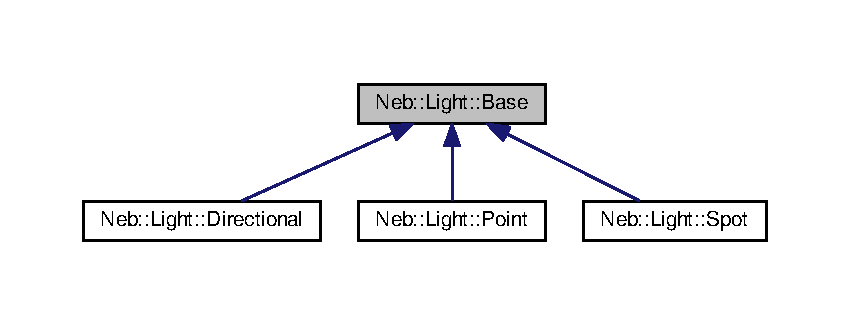
\includegraphics[width=350pt]{classNeb_1_1Light_1_1Base__inherit__graph}
\end{center}
\end{figure}


\-Collaboration diagram for \-Neb\-:\-:\-Light\-:\-:\-Base\-:\nopagebreak
\begin{figure}[H]
\begin{center}
\leavevmode
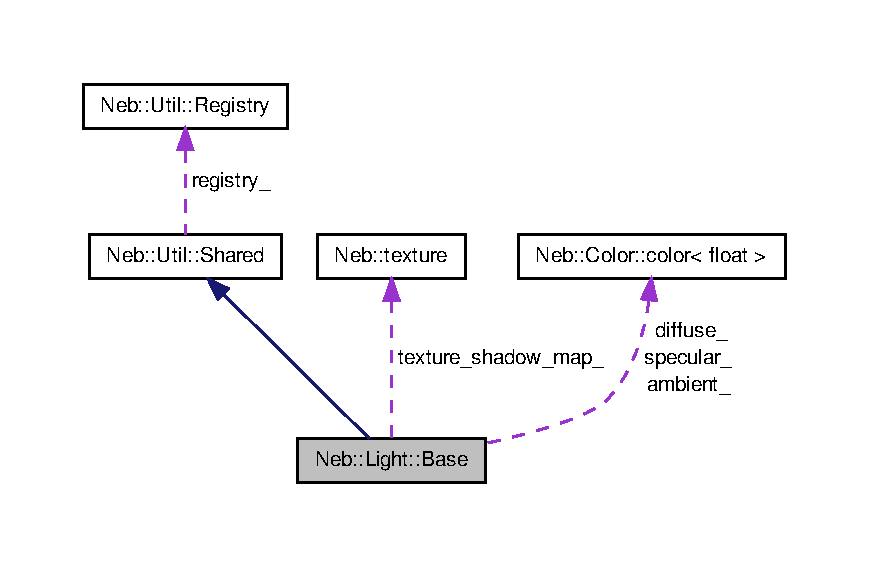
\includegraphics[width=350pt]{classNeb_1_1Light_1_1Base__coll__graph}
\end{center}
\end{figure}
\subsection*{\-Public \-Member \-Functions}
\begin{DoxyCompactItemize}
\item 
\hypertarget{classNeb_1_1Light_1_1Base_ab76457ec9dca523cd4e24f71b2602139}{{\bfseries \-Base} (\-Neb\-::\-Light\-::\-Util\-::\-Parent\-\_\-s)}\label{classNeb_1_1Light_1_1Base_ab76457ec9dca523cd4e24f71b2602139}

\item 
\hypertarget{classNeb_1_1Light_1_1Base_a4a9c112c52805f2c7a5b33d0f07171be}{void {\bfseries init} ()}\label{classNeb_1_1Light_1_1Base_a4a9c112c52805f2c7a5b33d0f07171be}

\item 
\hypertarget{classNeb_1_1Light_1_1Base_abe888a496b2e7316e2f04e21d324d132}{virtual void {\bfseries release} ()}\label{classNeb_1_1Light_1_1Base_abe888a496b2e7316e2f04e21d324d132}

\item 
\hypertarget{classNeb_1_1Light_1_1Base_a3f309821eb418f783f6fdb6cdfb4fef6}{virtual void {\bfseries cleanup} ()}\label{classNeb_1_1Light_1_1Base_a3f309821eb418f783f6fdb6cdfb4fef6}

\item 
\hypertarget{classNeb_1_1Light_1_1Base_afca74a5b128bb6940214ecdeafa50d04}{void {\bfseries step} (double)}\label{classNeb_1_1Light_1_1Base_afca74a5b128bb6940214ecdeafa50d04}

\item 
void \hyperlink{classNeb_1_1Light_1_1Base_ad621061e0be86708f0cbf7e300bc0c1e}{load} (int, physx\-::\-Px\-Mat44)
\item 
\hypertarget{classNeb_1_1Light_1_1Base_a903492950fc35bcfdafcbb91d42dddf2}{void {\bfseries load\-\_\-shadow} ()}\label{classNeb_1_1Light_1_1Base_a903492950fc35bcfdafcbb91d42dddf2}

\item 
\hypertarget{classNeb_1_1Light_1_1Base_af8a85af5b35db73ee6e260eb5d16ec0b}{void {\bfseries draw} ()}\label{classNeb_1_1Light_1_1Base_af8a85af5b35db73ee6e260eb5d16ec0b}

\item 
\hypertarget{classNeb_1_1Light_1_1Base_a0f2d5367bfdcb1911153bd4a21c26e50}{void {\bfseries dim} ()}\label{classNeb_1_1Light_1_1Base_a0f2d5367bfdcb1911153bd4a21c26e50}

\item 
\hypertarget{classNeb_1_1Light_1_1Base_a132bb5f66b3b590aa55f53ee17a67c4a}{void {\bfseries \-Render\-Shadow\-Post} ()}\label{classNeb_1_1Light_1_1Base_a132bb5f66b3b590aa55f53ee17a67c4a}

\item 
\hypertarget{classNeb_1_1Light_1_1Base_aac6c4177c6fd3b4f8773b0d431203ccc}{void {\bfseries \-Render\-Light\-P\-O\-V} ()}\label{classNeb_1_1Light_1_1Base_aac6c4177c6fd3b4f8773b0d431203ccc}

\item 
\hypertarget{classNeb_1_1Light_1_1Base_a45e032e7aa7203c0832d52949e14141c}{void {\bfseries notify\-\_\-foundation\-\_\-change\-\_\-pose} ()}\label{classNeb_1_1Light_1_1Base_a45e032e7aa7203c0832d52949e14141c}

\item 
\hypertarget{classNeb_1_1Light_1_1Base_a78c4664de9ddf719dea72d00fa8498a4}{physx\-::\-Px\-Mat44 {\bfseries get\-\_\-pose} ()}\label{classNeb_1_1Light_1_1Base_a78c4664de9ddf719dea72d00fa8498a4}

\item 
\hypertarget{classNeb_1_1Light_1_1Base_a125c8d3d4795bcec4ec546d82686bf38}{physx\-::\-Px\-Vec4 {\bfseries get\-\_\-pos} ()}\label{classNeb_1_1Light_1_1Base_a125c8d3d4795bcec4ec546d82686bf38}

\item 
\hypertarget{classNeb_1_1Light_1_1Base_ac8b71e530696633d24137c4d5d695af5}{virtual void {\bfseries load} (boost\-::archive\-::polymorphic\-\_\-iarchive \&ar, unsigned int const \&version)}\label{classNeb_1_1Light_1_1Base_ac8b71e530696633d24137c4d5d695af5}

\item 
\hypertarget{classNeb_1_1Light_1_1Base_a4e83a340a8c97d92da3bf3165bc4b176}{virtual void {\bfseries save} (boost\-::archive\-::polymorphic\-\_\-oarchive \&ar, unsigned int const \&version)}\label{classNeb_1_1Light_1_1Base_a4e83a340a8c97d92da3bf3165bc4b176}

\item 
\hypertarget{classNeb_1_1Light_1_1Base_a54780bbb4d3ce64a6151c20b1f72f6ef}{virtual void {\bfseries load\-Light\-Base} (boost\-::archive\-::polymorphic\-\_\-iarchive \&ar, unsigned int const \&version)=0}\label{classNeb_1_1Light_1_1Base_a54780bbb4d3ce64a6151c20b1f72f6ef}

\item 
\hypertarget{classNeb_1_1Light_1_1Base_a83fd19d93bf401dd11f9fd30eb9ba7dc}{virtual void {\bfseries save\-Light\-Base} (boost\-::archive\-::polymorphic\-\_\-oarchive \&ar, unsigned int const \&version)=0}\label{classNeb_1_1Light_1_1Base_a83fd19d93bf401dd11f9fd30eb9ba7dc}

\end{DoxyCompactItemize}
\subsection*{\-Public \-Attributes}
\begin{DoxyCompactItemize}
\item 
\hypertarget{classNeb_1_1Light_1_1Base_ab1526ac73c6c908f9c21499dfb45c44e}{\-Neb\-::\-Light\-::\-Util\-::\-Parent\-\_\-s {\bfseries parent\-\_\-}}\label{classNeb_1_1Light_1_1Base_ab1526ac73c6c908f9c21499dfb45c44e}

\item 
\hypertarget{classNeb_1_1Light_1_1Base_a3177179e3818a45a3c46dcb3fec2f367}{\-Neb\-::\-Light\-::\-Util\-::\-Flag {\bfseries flag\-\_\-}}\label{classNeb_1_1Light_1_1Base_a3177179e3818a45a3c46dcb3fec2f367}

\item 
\hypertarget{classNeb_1_1Light_1_1Base_a7d70167b9bd230b67c9aa843375ca0f2}{physx\-::\-Px\-Vec4 {\bfseries pos\-\_\-}}\label{classNeb_1_1Light_1_1Base_a7d70167b9bd230b67c9aa843375ca0f2}

\item 
\hypertarget{classNeb_1_1Light_1_1Base_a7251851266b83b2796e4c41069b5e7a4}{\hyperlink{classNeb_1_1Color_1_1color}{\-Neb\-::\-Color\-::color}$<$ float $>$ {\bfseries ambient\-\_\-}}\label{classNeb_1_1Light_1_1Base_a7251851266b83b2796e4c41069b5e7a4}

\item 
\hypertarget{classNeb_1_1Light_1_1Base_a34044e92e9ffdcedabc3c6194db0d4fc}{\hyperlink{classNeb_1_1Color_1_1color}{\-Neb\-::\-Color\-::color}$<$ float $>$ {\bfseries diffuse\-\_\-}}\label{classNeb_1_1Light_1_1Base_a34044e92e9ffdcedabc3c6194db0d4fc}

\item 
\hypertarget{classNeb_1_1Light_1_1Base_aee8554a23529297eb52c8b01e5bc0fea}{\hyperlink{classNeb_1_1Color_1_1color}{\-Neb\-::\-Color\-::color}$<$ float $>$ {\bfseries specular\-\_\-}}\label{classNeb_1_1Light_1_1Base_aee8554a23529297eb52c8b01e5bc0fea}

\item 
\hypertarget{classNeb_1_1Light_1_1Base_a62fdcf973dced05a726b4f196bc9a3d2}{float {\bfseries atten\-\_\-const\-\_\-}}\label{classNeb_1_1Light_1_1Base_a62fdcf973dced05a726b4f196bc9a3d2}

\item 
\hypertarget{classNeb_1_1Light_1_1Base_a13d0c44ef6f46d42d608997a37401744}{float {\bfseries atten\-\_\-linear\-\_\-}}\label{classNeb_1_1Light_1_1Base_a13d0c44ef6f46d42d608997a37401744}

\item 
\hypertarget{classNeb_1_1Light_1_1Base_ae5e40a74cc0cadaefe2aad8945d324db}{float {\bfseries atten\-\_\-quad\-\_\-}}\label{classNeb_1_1Light_1_1Base_ae5e40a74cc0cadaefe2aad8945d324db}

\item 
\hypertarget{classNeb_1_1Light_1_1Base_a45d18dc3beeec6a5ae06e33cb2ada2fb}{\hyperlink{classNeb_1_1texture}{texture} {\bfseries texture\-\_\-shadow\-\_\-map\-\_\-}}\label{classNeb_1_1Light_1_1Base_a45d18dc3beeec6a5ae06e33cb2ada2fb}

\end{DoxyCompactItemize}
\subsection*{\-Private \-Member \-Functions}
\begin{DoxyCompactItemize}
\item 
\hypertarget{classNeb_1_1Light_1_1Base_aa1038a031c1c7a280afe8d00bf41f00a}{{\footnotesize template$<$class Archive $>$ }\\void {\bfseries serialize\-Template} (\-Archive \&ar, unsigned int const \&version)}\label{classNeb_1_1Light_1_1Base_aa1038a031c1c7a280afe8d00bf41f00a}

\end{DoxyCompactItemize}


\subsection{\-Member \-Function \-Documentation}
\hypertarget{classNeb_1_1Light_1_1Base_ad621061e0be86708f0cbf7e300bc0c1e}{\index{\-Neb\-::\-Light\-::\-Base@{\-Neb\-::\-Light\-::\-Base}!load@{load}}
\index{load@{load}!Neb::Light::Base@{\-Neb\-::\-Light\-::\-Base}}
\subsubsection[{load}]{\setlength{\rightskip}{0pt plus 5cm}void {\bf \-Neb\-::\-Light\-::\-Base\-::load} (
\begin{DoxyParamCaption}
\item[{int}]{o, }
\item[{physx\-::\-Px\-Mat44}]{space}
\end{DoxyParamCaption}
)}}\label{classNeb_1_1Light_1_1Base_ad621061e0be86708f0cbf7e300bc0c1e}
\begin{DoxyRefDesc}{\-Todo}
\item[\hyperlink{todo__todo000011}{\-Todo}]way to ditinguish lights in shader \end{DoxyRefDesc}


\-The documentation for this class was generated from the following files\-:\begin{DoxyCompactItemize}
\item 
src/\-Nebula/\-Graphics/\-Light/\-Base.\-hh\item 
src/\-Nebula/\-Graphics/\-Light/\-Base.\-cc\end{DoxyCompactItemize}

\hypertarget{classNeb_1_1Camera_1_1Projection_1_1Base}{\section{\-Neb\-:\-:\-Camera\-:\-:\-Projection\-:\-:\-Base \-Class \-Reference}
\label{classNeb_1_1Camera_1_1Projection_1_1Base}\index{\-Neb\-::\-Camera\-::\-Projection\-::\-Base@{\-Neb\-::\-Camera\-::\-Projection\-::\-Base}}
}


 




{\ttfamily \#include $<$\-Perspective.\-hpp$>$}



\-Inheritance diagram for \-Neb\-:\-:\-Camera\-:\-:\-Projection\-:\-:\-Base\-:\nopagebreak
\begin{figure}[H]
\begin{center}
\leavevmode
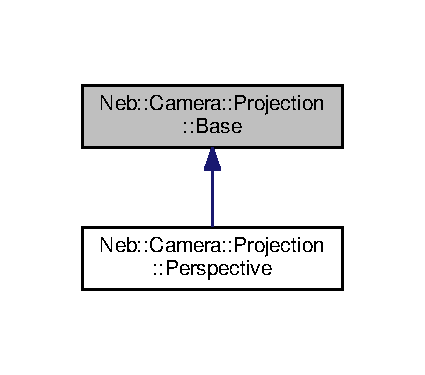
\includegraphics[width=262pt]{classNeb_1_1Camera_1_1Projection_1_1Base__inherit__graph}
\end{center}
\end{figure}
\subsection*{\-Public \-Member \-Functions}
\begin{DoxyCompactItemize}
\item 
\hypertarget{classNeb_1_1Camera_1_1Projection_1_1Base_a2bf5d7b2b444e405540d1ba3a1dadf87}{\hyperlink{classNeb_1_1Camera_1_1Projection_1_1Base_a2bf5d7b2b444e405540d1ba3a1dadf87}{\-Base} (std\-::shared\-\_\-ptr$<$ \hyperlink{classNeb_1_1renderable}{\-Neb\-::renderable} $>$)}\label{classNeb_1_1Camera_1_1Projection_1_1Base_a2bf5d7b2b444e405540d1ba3a1dadf87}

\begin{DoxyCompactList}\small\item\em \-Constructor. \end{DoxyCompactList}\item 
\hypertarget{classNeb_1_1Camera_1_1Projection_1_1Base_a4101febf5b6540d5e29b9209bcc33f74}{virtual physx\-::\-Px\-Mat44 {\bfseries proj} ()=0}\label{classNeb_1_1Camera_1_1Projection_1_1Base_a4101febf5b6540d5e29b9209bcc33f74}

\item 
\hypertarget{classNeb_1_1Camera_1_1Projection_1_1Base_a4d348ea3fc3134598b02d373a8d081d5}{void {\bfseries load} ()}\label{classNeb_1_1Camera_1_1Projection_1_1Base_a4d348ea3fc3134598b02d373a8d081d5}

\item 
void \hyperlink{classNeb_1_1Camera_1_1Projection_1_1Base_a7a0ef0507f546a0da56bb596de53c962}{step} (double)
\begin{DoxyCompactList}\small\item\em step \end{DoxyCompactList}\end{DoxyCompactItemize}
\begin{Indent}{\bf \-Accessors @\{}\par
\begin{DoxyCompactItemize}
\item 
\hypertarget{classNeb_1_1Camera_1_1Projection_1_1Base_a341df0c373f2c137f37cc9bfab3d00fd}{\-Neb\-::window\-::window\-\_\-s \hyperlink{classNeb_1_1Camera_1_1Projection_1_1Base_a341df0c373f2c137f37cc9bfab3d00fd}{get\-Window} ()}\label{classNeb_1_1Camera_1_1Projection_1_1Base_a341df0c373f2c137f37cc9bfab3d00fd}

\begin{DoxyCompactList}\small\item\em \-Get parent window. \end{DoxyCompactList}\end{DoxyCompactItemize}
\end{Indent}
\subsection*{\-Protected \-Attributes}
\begin{DoxyCompactItemize}
\item 
\hypertarget{classNeb_1_1Camera_1_1Projection_1_1Base_a5e6e0c80197f7e6e1f3d35b57c9b4dcb}{std\-::weak\-\_\-ptr$<$ \hyperlink{classNeb_1_1renderable}{renderable} $>$ \hyperlink{classNeb_1_1Camera_1_1Projection_1_1Base_a5e6e0c80197f7e6e1f3d35b57c9b4dcb}{renderable\-\_\-}}\label{classNeb_1_1Camera_1_1Projection_1_1Base_a5e6e0c80197f7e6e1f3d35b57c9b4dcb}

\begin{DoxyCompactList}\small\item\em \-Parent. \end{DoxyCompactList}\end{DoxyCompactItemize}


\subsection{\-Detailed \-Description}


\subsection{\-Member \-Function \-Documentation}
\hypertarget{classNeb_1_1Camera_1_1Projection_1_1Base_a7a0ef0507f546a0da56bb596de53c962}{\index{\-Neb\-::\-Camera\-::\-Projection\-::\-Base@{\-Neb\-::\-Camera\-::\-Projection\-::\-Base}!step@{step}}
\index{step@{step}!Neb::Camera::Projection::Base@{\-Neb\-::\-Camera\-::\-Projection\-::\-Base}}
\subsubsection[{step}]{\setlength{\rightskip}{0pt plus 5cm}void {\bf \-Neb\-::\-Camera\-::\-Projection\-::\-Base\-::step} (
\begin{DoxyParamCaption}
\item[{double}]{}
\end{DoxyParamCaption}
)}}\label{classNeb_1_1Camera_1_1Projection_1_1Base_a7a0ef0507f546a0da56bb596de53c962}


step 

\begin{DoxyRefDesc}{\-Todo}
\item[\hyperlink{todo__todo000005}{\-Todo}]explain when in timeline this occurs and in which thread and why \end{DoxyRefDesc}


\-Reimplemented in \hyperlink{classNeb_1_1Camera_1_1Projection_1_1Perspective_a74771031b253ee639dff1a15e6b9c32d}{\-Neb\-::\-Camera\-::\-Projection\-::\-Perspective}.



\-The documentation for this class was generated from the following files\-:\begin{DoxyCompactItemize}
\item 
src/\-Nebula/\-Graphics/\-Camera/\-Projection/\-Perspective.\-hpp\item 
src/\-Nebula/\-Graphics/\-Camera/\-Projection/\-Perspective.\-cpp\end{DoxyCompactItemize}

\hypertarget{classNeb_1_1Camera_1_1View_1_1Base}{\section{\-Neb\-:\-:\-Camera\-:\-:\-View\-:\-:\-Base \-Class \-Reference}
\label{classNeb_1_1Camera_1_1View_1_1Base}\index{\-Neb\-::\-Camera\-::\-View\-::\-Base@{\-Neb\-::\-Camera\-::\-View\-::\-Base}}
}


 




{\ttfamily \#include $<$\-Base.\-hpp$>$}



\-Inheritance diagram for \-Neb\-:\-:\-Camera\-:\-:\-View\-:\-:\-Base\-:
\nopagebreak
\begin{figure}[H]
\begin{center}
\leavevmode
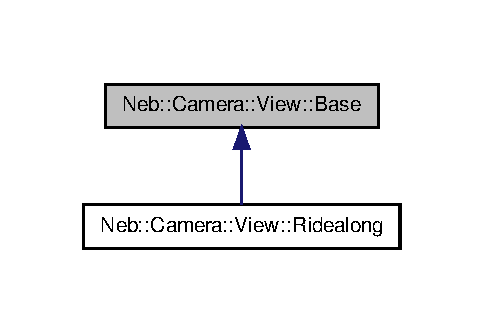
\includegraphics[width=232pt]{classNeb_1_1Camera_1_1View_1_1Base__inherit__graph}
\end{center}
\end{figure}
\subsection*{\-Public \-Member \-Functions}
\begin{DoxyCompactItemize}
\item 
\hypertarget{classNeb_1_1Camera_1_1View_1_1Base_a4824e00fe745e7d7b6bef00daaf6f191}{\hyperlink{classNeb_1_1Camera_1_1View_1_1Base_a4824e00fe745e7d7b6bef00daaf6f191}{\-Base} ()}\label{classNeb_1_1Camera_1_1View_1_1Base_a4824e00fe745e7d7b6bef00daaf6f191}

\begin{DoxyCompactList}\small\item\em \-Constructor. \end{DoxyCompactList}\item 
\hypertarget{classNeb_1_1Camera_1_1View_1_1Base_a55338f0f215524b7c026fff7d08bbdcb}{void \hyperlink{classNeb_1_1Camera_1_1View_1_1Base_a55338f0f215524b7c026fff7d08bbdcb}{load} ()}\label{classNeb_1_1Camera_1_1View_1_1Base_a55338f0f215524b7c026fff7d08bbdcb}

\begin{DoxyCompactList}\small\item\em \-Load view matrix into \-G\-L\-S\-L. \end{DoxyCompactList}\item 
\hypertarget{classNeb_1_1Camera_1_1View_1_1Base_ad7609a0b61cd9fb9c54cb3b01335b764}{virtual physx\-::\-Px\-Mat44 \hyperlink{classNeb_1_1Camera_1_1View_1_1Base_ad7609a0b61cd9fb9c54cb3b01335b764}{view} ()=0}\label{classNeb_1_1Camera_1_1View_1_1Base_ad7609a0b61cd9fb9c54cb3b01335b764}

\begin{DoxyCompactList}\small\item\em \-Get view matrix. \end{DoxyCompactList}\item 
virtual void \hyperlink{classNeb_1_1Camera_1_1View_1_1Base_aa3c5978efc6cd916f0f91bb8def375c5}{step} (double)=0
\begin{DoxyCompactList}\small\item\em \-Step. \end{DoxyCompactList}\end{DoxyCompactItemize}
\subsection*{\-Public \-Attributes}
\begin{DoxyCompactItemize}
\item 
\hypertarget{classNeb_1_1Camera_1_1View_1_1Base_a931b1ed0302ee399c970740177c2e2de}{double \hyperlink{classNeb_1_1Camera_1_1View_1_1Base_a931b1ed0302ee399c970740177c2e2de}{last\-\_\-}}\label{classNeb_1_1Camera_1_1View_1_1Base_a931b1ed0302ee399c970740177c2e2de}

\begin{DoxyCompactList}\small\item\em \-Time of last step. \end{DoxyCompactList}\end{DoxyCompactItemize}


\subsection{\-Detailed \-Description}


\subsection{\-Member \-Function \-Documentation}
\hypertarget{classNeb_1_1Camera_1_1View_1_1Base_aa3c5978efc6cd916f0f91bb8def375c5}{\index{\-Neb\-::\-Camera\-::\-View\-::\-Base@{\-Neb\-::\-Camera\-::\-View\-::\-Base}!step@{step}}
\index{step@{step}!Neb::Camera::View::Base@{\-Neb\-::\-Camera\-::\-View\-::\-Base}}
\subsubsection[{step}]{\setlength{\rightskip}{0pt plus 5cm}virtual void {\bf \-Neb\-::\-Camera\-::\-View\-::\-Base\-::step} (
\begin{DoxyParamCaption}
\item[{double}]{}
\end{DoxyParamCaption}
)\hspace{0.3cm}{\ttfamily  \mbox{[}pure virtual\mbox{]}}}}\label{classNeb_1_1Camera_1_1View_1_1Base_aa3c5978efc6cd916f0f91bb8def375c5}


\-Step. 

\begin{DoxyRefDesc}{\-Todo}
\item[\hyperlink{todo__todo000004}{\-Todo}]explain when in timeline this occurs and in which thread and why \end{DoxyRefDesc}


\-Implemented in \hyperlink{classNeb_1_1Camera_1_1View_1_1Ridealong_a11898b9a6acd7ca864c0a32f12ec6e12}{\-Neb\-::\-Camera\-::\-View\-::\-Ridealong}.



\-The documentation for this class was generated from the following file\-:\begin{DoxyCompactItemize}
\item 
src/\-Nebula/\-Graphics/\-Camera/\-View/\-Base.\-hpp\end{DoxyCompactItemize}

\hypertarget{classNeb_1_1Graphics_1_1Window_1_1Base}{\section{\-Neb\-:\-:\-Graphics\-:\-:\-Window\-:\-:\-Base \-Class \-Reference}
\label{classNeb_1_1Graphics_1_1Window_1_1Base}\index{\-Neb\-::\-Graphics\-::\-Window\-::\-Base@{\-Neb\-::\-Graphics\-::\-Window\-::\-Base}}
}


\-Inheritance diagram for \-Neb\-:\-:\-Graphics\-:\-:\-Window\-:\-:\-Base\-:\nopagebreak
\begin{figure}[H]
\begin{center}
\leavevmode
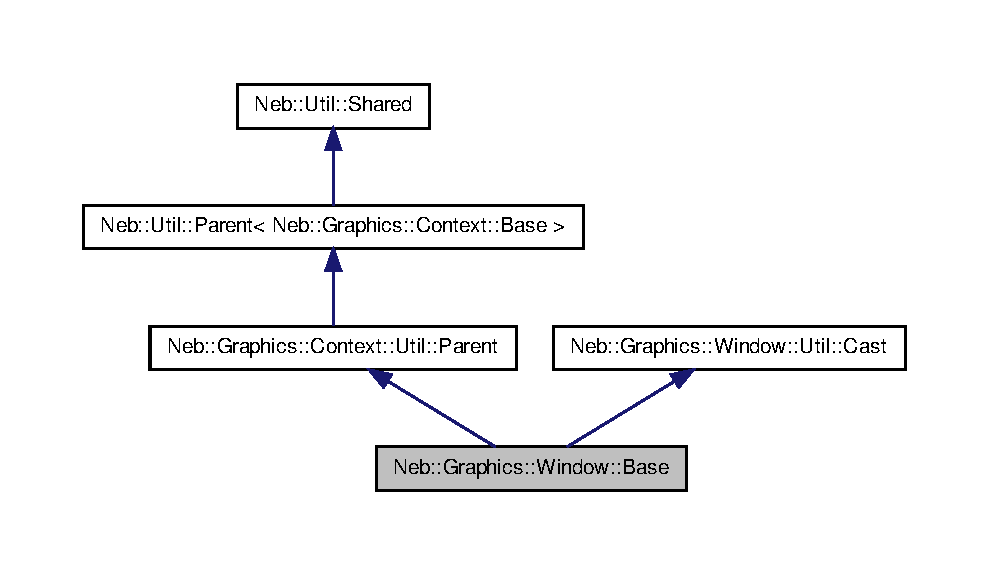
\includegraphics[width=350pt]{classNeb_1_1Graphics_1_1Window_1_1Base__inherit__graph}
\end{center}
\end{figure}


\-Collaboration diagram for \-Neb\-:\-:\-Graphics\-:\-:\-Window\-:\-:\-Base\-:\nopagebreak
\begin{figure}[H]
\begin{center}
\leavevmode
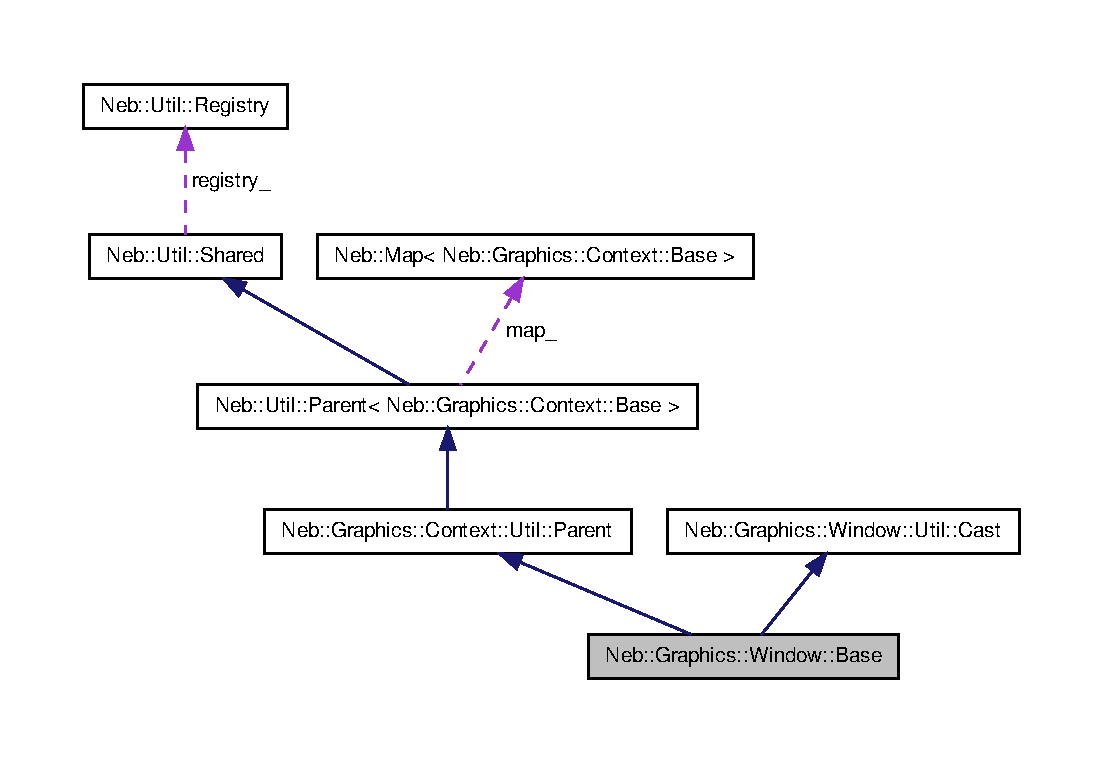
\includegraphics[width=350pt]{classNeb_1_1Graphics_1_1Window_1_1Base__coll__graph}
\end{center}
\end{figure}
\subsection*{\-Classes}
\begin{DoxyCompactItemize}
\item 
struct \hyperlink{structNeb_1_1Graphics_1_1Window_1_1Base_1_1flag}{flag}
\end{DoxyCompactItemize}
\subsection*{\-Public \-Member \-Functions}
\begin{DoxyCompactItemize}
\item 
\hyperlink{classNeb_1_1Graphics_1_1Window_1_1Base_ac71945a8c24260d3427539bdd6c9bc6b}{\-Base} ()
\item 
\hypertarget{classNeb_1_1Graphics_1_1Window_1_1Base_a8e3c37aa30e0a2a2c4998753dfa27a3e}{{\bfseries \-Base} (\-Neb\-::\-Graphics\-::\-Window\-::\-Util\-::\-Parent\-\_\-s parent)}\label{classNeb_1_1Graphics_1_1Window_1_1Base_a8e3c37aa30e0a2a2c4998753dfa27a3e}

\item 
\hypertarget{classNeb_1_1Graphics_1_1Window_1_1Base_a78d20e60f26c917ed0fb4a2f9c685f6e}{virtual void {\bfseries init} ()}\label{classNeb_1_1Graphics_1_1Window_1_1Base_a78d20e60f26c917ed0fb4a2f9c685f6e}

\item 
\hypertarget{classNeb_1_1Graphics_1_1Window_1_1Base_aa8da9aa63c93c369216a2af313b94e01}{virtual void {\bfseries release} ()}\label{classNeb_1_1Graphics_1_1Window_1_1Base_aa8da9aa63c93c369216a2af313b94e01}

\item 
\hypertarget{classNeb_1_1Graphics_1_1Window_1_1Base_a16653d78a1cdbabc441bd774e8add7cd}{void {\bfseries resize} ()}\label{classNeb_1_1Graphics_1_1Window_1_1Base_a16653d78a1cdbabc441bd774e8add7cd}

\item 
\hypertarget{classNeb_1_1Graphics_1_1Window_1_1Base_ae259e99c30c251c05534b60760ce0afe}{void {\bfseries callback\-\_\-window\-\_\-pos\-\_\-fun} (\-G\-L\-F\-Wwindow $\ast$, int, int)}\label{classNeb_1_1Graphics_1_1Window_1_1Base_ae259e99c30c251c05534b60760ce0afe}

\item 
\hypertarget{classNeb_1_1Graphics_1_1Window_1_1Base_aa017187b6688141211d6bc5e55aa177a}{void {\bfseries callback\-\_\-window\-\_\-size\-\_\-fun} (\-G\-L\-F\-Wwindow $\ast$, int, int)}\label{classNeb_1_1Graphics_1_1Window_1_1Base_aa017187b6688141211d6bc5e55aa177a}

\item 
\hypertarget{classNeb_1_1Graphics_1_1Window_1_1Base_abb8bb12eacf4e20902af01c06a37cca8}{void {\bfseries callback\-\_\-window\-\_\-close\-\_\-fun} (\-G\-L\-F\-Wwindow $\ast$)}\label{classNeb_1_1Graphics_1_1Window_1_1Base_abb8bb12eacf4e20902af01c06a37cca8}

\item 
\hypertarget{classNeb_1_1Graphics_1_1Window_1_1Base_aa369484b62b908065055164d2886e840}{void {\bfseries callback\-\_\-window\-\_\-refresh\-\_\-fun} (\-G\-L\-F\-Wwindow $\ast$)}\label{classNeb_1_1Graphics_1_1Window_1_1Base_aa369484b62b908065055164d2886e840}

\item 
\hypertarget{classNeb_1_1Graphics_1_1Window_1_1Base_a4066dcc28ad3783ab3f7fa3ebc1ac82d}{void {\bfseries callback\-\_\-mouse\-\_\-button\-\_\-fun} (\-G\-L\-F\-Wwindow $\ast$, int, int, int)}\label{classNeb_1_1Graphics_1_1Window_1_1Base_a4066dcc28ad3783ab3f7fa3ebc1ac82d}

\item 
\hypertarget{classNeb_1_1Graphics_1_1Window_1_1Base_a5cb1f1c50b2fd077c557ff6967288fba}{void {\bfseries callback\-\_\-key\-\_\-fun} (\-G\-L\-F\-Wwindow $\ast$, int, int, int, int)}\label{classNeb_1_1Graphics_1_1Window_1_1Base_a5cb1f1c50b2fd077c557ff6967288fba}

\end{DoxyCompactItemize}
\begin{Indent}{\bf \-Main \-Loop @\{}\par
\begin{DoxyCompactItemize}
\item 
void \hyperlink{classNeb_1_1Graphics_1_1Window_1_1Base_adc53fbf523d1dab863f767c5cb534a77}{render} (double time)
\item 
\hypertarget{classNeb_1_1Graphics_1_1Window_1_1Base_a2fd329c3b4f33590a9e26acf1affcb8d}{void {\bfseries step} (double time)}\label{classNeb_1_1Graphics_1_1Window_1_1Base_a2fd329c3b4f33590a9e26acf1affcb8d}

\end{DoxyCompactItemize}
\end{Indent}
\subsection*{\-Public \-Attributes}
\begin{DoxyCompactItemize}
\item 
\hypertarget{classNeb_1_1Graphics_1_1Window_1_1Base_a14a238f206643db3b8d8ebb5c9f745fd}{\-Neb\-::\-Graphics\-::\-Window\-::\-Util\-::\-Parent\-\_\-s {\bfseries parent\-\_\-}}\label{classNeb_1_1Graphics_1_1Window_1_1Base_a14a238f206643db3b8d8ebb5c9f745fd}

\item 
\hypertarget{classNeb_1_1Graphics_1_1Window_1_1Base_a3369e968d1b20a9dd7a4df3fcbd98eab}{\begin{tabbing}
xx\=xx\=xx\=xx\=xx\=xx\=xx\=xx\=xx\=\kill
struct \{\\
\>Neb::Signals::KeyFun {\bfseries key\_fun\_}\\
\>Neb::Signals::MouseButtonFun {\bfseries mouse\_button\_fun\_}\\
\} {\bfseries sig\_}}\label{classNeb_1_1Graphics_1_1Window_1_1Base_a3369e968d1b20a9dd7a4df3fcbd98eab}
\\

\end{tabbing}\item 
\hypertarget{classNeb_1_1Graphics_1_1Window_1_1Base_aaf83a17ebde0592bec931ba053d8e98d}{\-Neb\-::\-Graphics\-::\-Window\-::\-Util\-::\-Flag {\bfseries flag\-\_\-}}\label{classNeb_1_1Graphics_1_1Window_1_1Base_aaf83a17ebde0592bec931ba053d8e98d}

\item 
\hypertarget{classNeb_1_1Graphics_1_1Window_1_1Base_a91656b0995fab99564762ed5b1160924}{int {\bfseries x\-\_\-}}\label{classNeb_1_1Graphics_1_1Window_1_1Base_a91656b0995fab99564762ed5b1160924}

\item 
\hypertarget{classNeb_1_1Graphics_1_1Window_1_1Base_afcdb8d2cdde0452c5e3bbe6f9a9a81d2}{int {\bfseries y\-\_\-}}\label{classNeb_1_1Graphics_1_1Window_1_1Base_afcdb8d2cdde0452c5e3bbe6f9a9a81d2}

\item 
\hypertarget{classNeb_1_1Graphics_1_1Window_1_1Base_a73d8621556c2a7310277ab5cb5df3e01}{int {\bfseries w\-\_\-}}\label{classNeb_1_1Graphics_1_1Window_1_1Base_a73d8621556c2a7310277ab5cb5df3e01}

\item 
\hypertarget{classNeb_1_1Graphics_1_1Window_1_1Base_a8d1b70980e3c8c7b4f690b89cccb8d0f}{int {\bfseries h\-\_\-}}\label{classNeb_1_1Graphics_1_1Window_1_1Base_a8d1b70980e3c8c7b4f690b89cccb8d0f}

\item 
\hypertarget{classNeb_1_1Graphics_1_1Window_1_1Base_adfd3a69ec14cc8c945076d18b7ab9574}{std\-::string {\bfseries title\-\_\-}}\label{classNeb_1_1Graphics_1_1Window_1_1Base_adfd3a69ec14cc8c945076d18b7ab9574}

\item 
\hypertarget{classNeb_1_1Graphics_1_1Window_1_1Base_a696431f4829005942769ddaf27043aee}{\-G\-L\-F\-Wwindow $\ast$ {\bfseries window\-\_\-}}\label{classNeb_1_1Graphics_1_1Window_1_1Base_a696431f4829005942769ddaf27043aee}

\end{DoxyCompactItemize}


\subsection{\-Constructor \& \-Destructor \-Documentation}
\hypertarget{classNeb_1_1Graphics_1_1Window_1_1Base_ac71945a8c24260d3427539bdd6c9bc6b}{\index{\-Neb\-::\-Graphics\-::\-Window\-::\-Base@{\-Neb\-::\-Graphics\-::\-Window\-::\-Base}!\-Base@{\-Base}}
\index{\-Base@{\-Base}!Neb::Graphics::Window::Base@{\-Neb\-::\-Graphics\-::\-Window\-::\-Base}}
\subsubsection[{\-Base}]{\setlength{\rightskip}{0pt plus 5cm}{\bf \-Neb\-::\-Graphics\-::\-Window\-::\-Base\-::\-Base} (
\begin{DoxyParamCaption}
{}
\end{DoxyParamCaption}
)}}\label{classNeb_1_1Graphics_1_1Window_1_1Base_ac71945a8c24260d3427539bdd6c9bc6b}
\begin{DoxyRefDesc}{\-Todo}
\item[\hyperlink{todo__todo000012}{\-Todo}]get rid of my unique ptr class. \-Just use private member and be careful not to pass around shared ptrs to things \end{DoxyRefDesc}


\subsection{\-Member \-Function \-Documentation}
\hypertarget{classNeb_1_1Graphics_1_1Window_1_1Base_adc53fbf523d1dab863f767c5cb534a77}{\index{\-Neb\-::\-Graphics\-::\-Window\-::\-Base@{\-Neb\-::\-Graphics\-::\-Window\-::\-Base}!render@{render}}
\index{render@{render}!Neb::Graphics::Window::Base@{\-Neb\-::\-Graphics\-::\-Window\-::\-Base}}
\subsubsection[{render}]{\setlength{\rightskip}{0pt plus 5cm}void {\bf \-Neb\-::\-Graphics\-::\-Window\-::\-Base\-::render} (
\begin{DoxyParamCaption}
\item[{double}]{time}
\end{DoxyParamCaption}
)}}\label{classNeb_1_1Graphics_1_1Window_1_1Base_adc53fbf523d1dab863f767c5cb534a77}
\begin{DoxyRefDesc}{\-Todo}
\item[\hyperlink{todo__todo000013}{\-Todo}]rendering multiple contexts in a window \end{DoxyRefDesc}


\-The documentation for this class was generated from the following files\-:\begin{DoxyCompactItemize}
\item 
src/\-Nebula/\-Graphics/\-Window/\-Base.\-hh\item 
src/\-Nebula/\-Graphics/\-Window/\-Base.\-cc\item 
src/\-Nebula/\-Shape/\-Base.\-cc\end{DoxyCompactItemize}

\hypertarget{classNeb_1_1Event_1_1Actor_1_1Base}{\section{\-Neb\-:\-:\-Event\-:\-:\-Actor\-:\-:\-Base \-Class \-Reference}
\label{classNeb_1_1Event_1_1Actor_1_1Base}\index{\-Neb\-::\-Event\-::\-Actor\-::\-Base@{\-Neb\-::\-Event\-::\-Actor\-::\-Base}}
}
\subsection*{\-Public \-Member \-Functions}
\begin{DoxyCompactItemize}
\item 
\hypertarget{classNeb_1_1Event_1_1Actor_1_1Base_a7e63345e09aa9a83dc10804d99759d6a}{{\footnotesize template$<$class Archive $>$ }\\void {\bfseries serialize} (\-Archive \&ar, unsigned int const \&version)}\label{classNeb_1_1Event_1_1Actor_1_1Base_a7e63345e09aa9a83dc10804d99759d6a}

\item 
\hypertarget{classNeb_1_1Event_1_1Actor_1_1Base_aa9cf29e608e5367af1006ceec717bbab}{virtual void {\bfseries serialize\-\_\-derived} (boost\-::archive\-::xml\-\_\-oarchive \&ar, unsigned int const \&version)=0}\label{classNeb_1_1Event_1_1Actor_1_1Base_aa9cf29e608e5367af1006ceec717bbab}

\item 
\hypertarget{classNeb_1_1Event_1_1Actor_1_1Base_ac4cc97711ed27e265ca977b89fa613e8}{virtual void {\bfseries serialize\-\_\-derived} (boost\-::archive\-::xml\-\_\-iarchive \&ar, unsigned int const \&version)=0}\label{classNeb_1_1Event_1_1Actor_1_1Base_ac4cc97711ed27e265ca977b89fa613e8}

\item 
\hypertarget{classNeb_1_1Event_1_1Actor_1_1Base_a41a75cb7ea7fc0bf463f2803ba3efa32}{virtual void {\bfseries serialize\-\_\-derived} (boost\-::archive\-::binary\-\_\-oarchive \&ar, unsigned int const \&version)=0}\label{classNeb_1_1Event_1_1Actor_1_1Base_a41a75cb7ea7fc0bf463f2803ba3efa32}

\item 
\hypertarget{classNeb_1_1Event_1_1Actor_1_1Base_a501859262708f2c72cf1a0bd20d803c7}{virtual void {\bfseries serialize\-\_\-derived} (boost\-::archive\-::binary\-\_\-iarchive \&ar, unsigned int const \&version)=0}\label{classNeb_1_1Event_1_1Actor_1_1Base_a501859262708f2c72cf1a0bd20d803c7}

\end{DoxyCompactItemize}
\subsection*{\-Static \-Public \-Attributes}
\begin{DoxyCompactItemize}
\item 
\hypertarget{classNeb_1_1Event_1_1Actor_1_1Base_ab6711b6cd077caa473f0c3b7416a265f}{static int {\bfseries hash\-\_\-code\-\_\-}}\label{classNeb_1_1Event_1_1Actor_1_1Base_ab6711b6cd077caa473f0c3b7416a265f}

\end{DoxyCompactItemize}


\-The documentation for this class was generated from the following file\-:\begin{DoxyCompactItemize}
\item 
src/gru/actor/event.\-hpp\end{DoxyCompactItemize}

\hypertarget{classNeb_1_1Actor_1_1Actor_1_1Base}{\section{Neb\-:\-:Actor\-:\-:Actor\-:\-:Base Class Reference}
\label{classNeb_1_1Actor_1_1Actor_1_1Base}\index{Neb\-::\-Actor\-::\-Actor\-::\-Base@{Neb\-::\-Actor\-::\-Actor\-::\-Base}}
}


Inheritance diagram for Neb\-:\-:Actor\-:\-:Actor\-:\-:Base\-:
\nopagebreak
\begin{figure}[H]
\begin{center}
\leavevmode
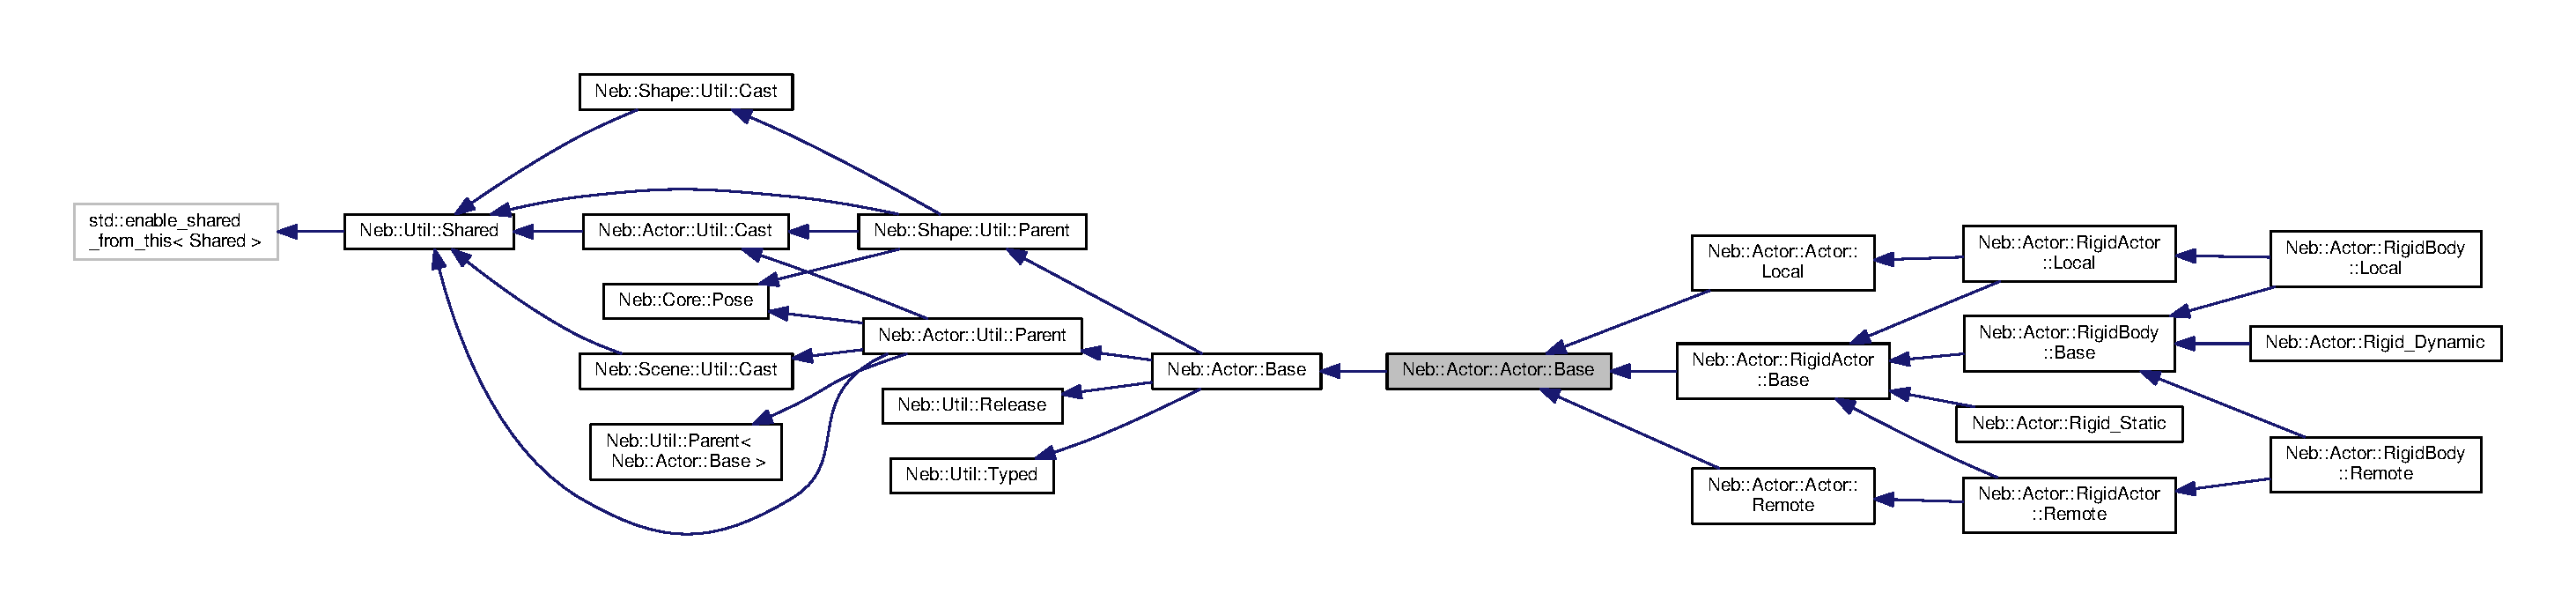
\includegraphics[width=350pt]{classNeb_1_1Actor_1_1Actor_1_1Base__inherit__graph}
\end{center}
\end{figure}


Collaboration diagram for Neb\-:\-:Actor\-:\-:Actor\-:\-:Base\-:
\nopagebreak
\begin{figure}[H]
\begin{center}
\leavevmode
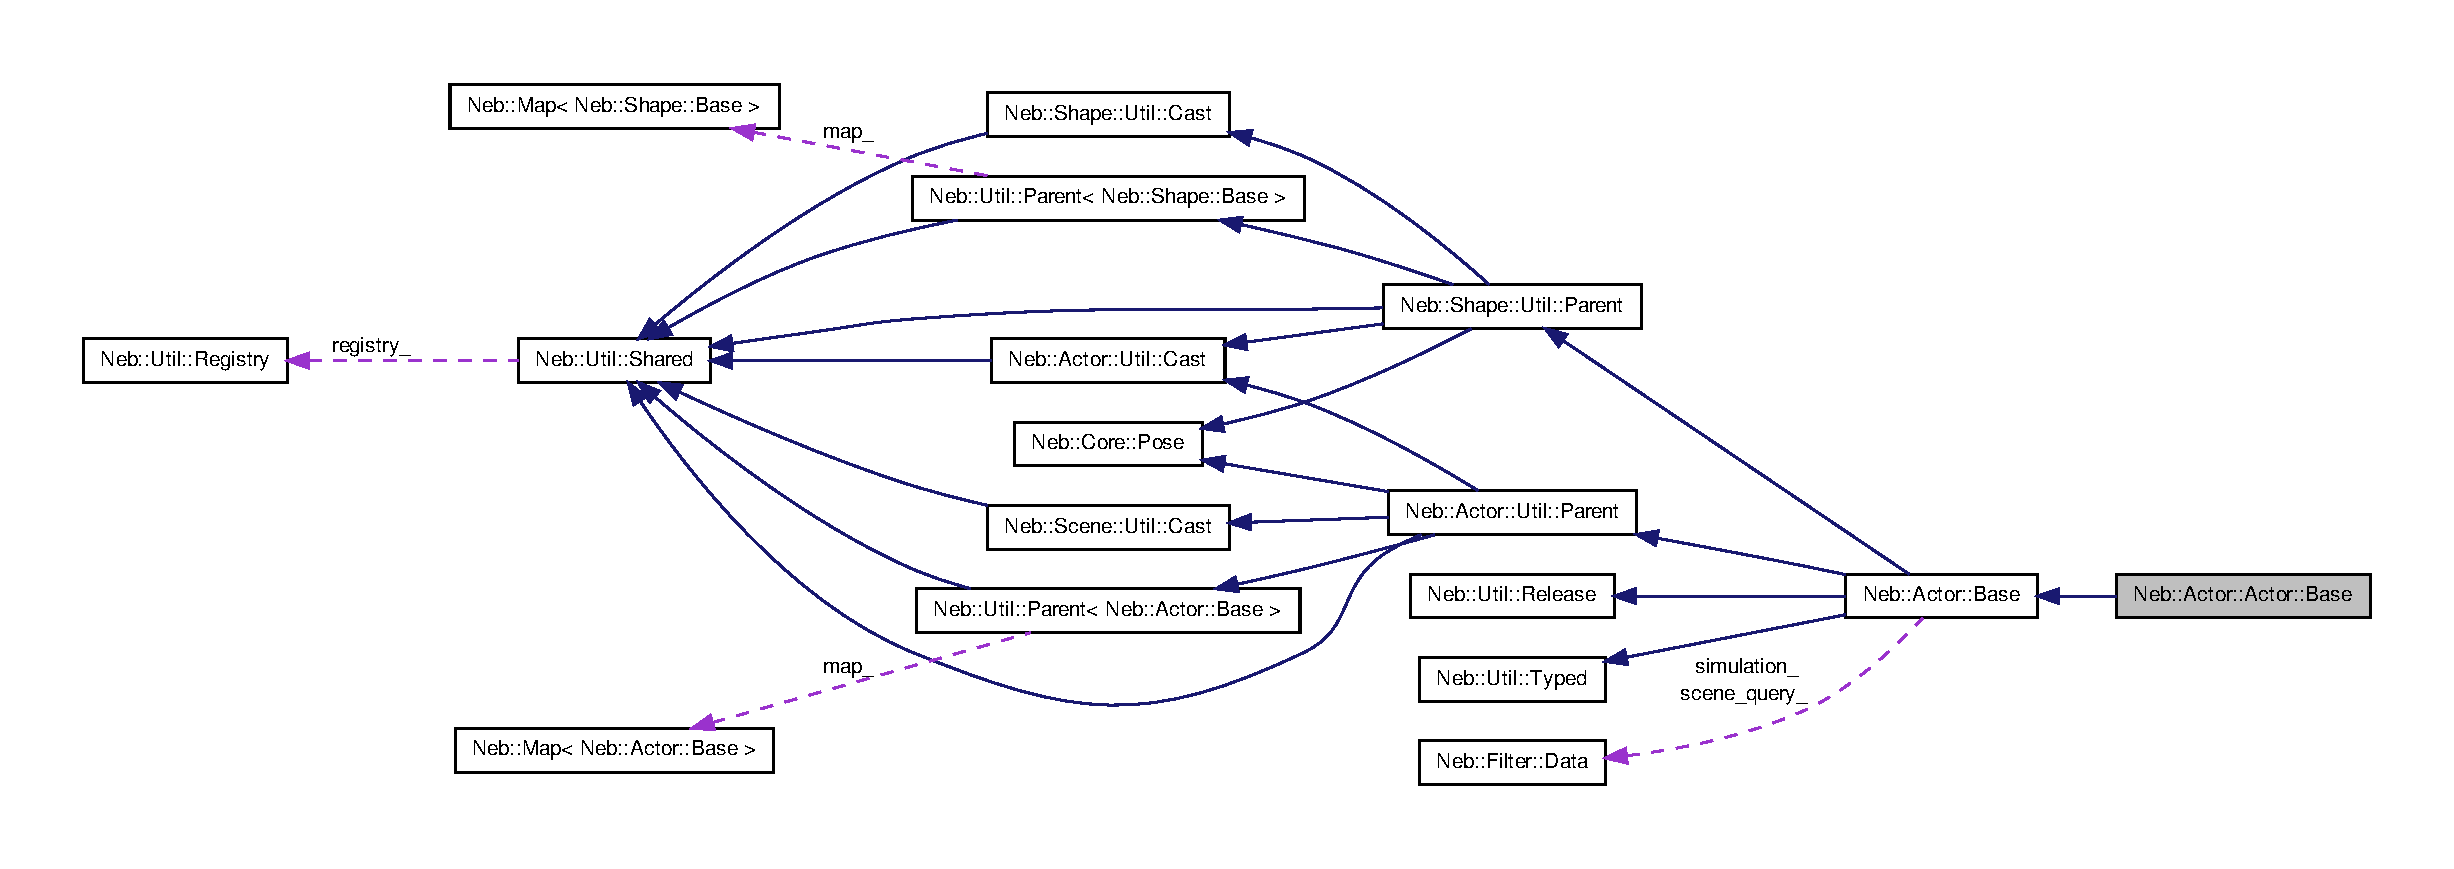
\includegraphics[width=350pt]{classNeb_1_1Actor_1_1Actor_1_1Base__coll__graph}
\end{center}
\end{figure}
\subsection*{Public Member Functions}
\begin{DoxyCompactItemize}
\item 
\hypertarget{classNeb_1_1Actor_1_1Actor_1_1Base_ac0c10d0555dc9d5e4bcc07f8159720df}{{\bfseries Base} (Neb\-::\-Actor\-::\-Util\-::\-Parent\-\_\-s)}\label{classNeb_1_1Actor_1_1Actor_1_1Base_ac0c10d0555dc9d5e4bcc07f8159720df}

\item 
\hypertarget{classNeb_1_1Actor_1_1Actor_1_1Base_a74b5eec0f243aa72bb9b642a353b3799}{virtual void {\bfseries init} ()}\label{classNeb_1_1Actor_1_1Actor_1_1Base_a74b5eec0f243aa72bb9b642a353b3799}

\item 
\hypertarget{classNeb_1_1Actor_1_1Actor_1_1Base_a1e7bc5de4a6b30c46a602a29c0face68}{virtual void {\bfseries release} ()}\label{classNeb_1_1Actor_1_1Actor_1_1Base_a1e7bc5de4a6b30c46a602a29c0face68}

\item 
\hypertarget{classNeb_1_1Actor_1_1Actor_1_1Base_a08e75988b2a5bb8dbcc279fce4d0c11d}{virtual void {\bfseries add\-\_\-force} (double)}\label{classNeb_1_1Actor_1_1Actor_1_1Base_a08e75988b2a5bb8dbcc279fce4d0c11d}

\item 
\hypertarget{classNeb_1_1Actor_1_1Actor_1_1Base_ac763835ed788dd6eac20dd72f3cf9169}{virtual void {\bfseries set\-\_\-pose} (physx\-::\-Px\-Transform)}\label{classNeb_1_1Actor_1_1Actor_1_1Base_ac763835ed788dd6eac20dd72f3cf9169}

\item 
\hypertarget{classNeb_1_1Actor_1_1Actor_1_1Base_a0ddaa61c1deaef77e07b898af73cb4af}{virtual int {\bfseries fire} ()}\label{classNeb_1_1Actor_1_1Actor_1_1Base_a0ddaa61c1deaef77e07b898af73cb4af}

\item 
\hypertarget{classNeb_1_1Actor_1_1Actor_1_1Base_a511a68cc306ce9e0b3417aa310eeae4f}{virtual Neb\-::\-Actor\-::\-Base\-\_\-s {\bfseries get\-\_\-projectile} ()=0}\label{classNeb_1_1Actor_1_1Actor_1_1Base_a511a68cc306ce9e0b3417aa310eeae4f}

\item 
\hypertarget{classNeb_1_1Actor_1_1Actor_1_1Base_ae514775e89a0c97b88c68a16dfba6796}{virtual void {\bfseries create\-\_\-physics} ()}\label{classNeb_1_1Actor_1_1Actor_1_1Base_ae514775e89a0c97b88c68a16dfba6796}

\item 
\hypertarget{classNeb_1_1Actor_1_1Actor_1_1Base_a7c88551377b004c027c92a752436d88e}{virtual void {\bfseries init\-\_\-physics} ()}\label{classNeb_1_1Actor_1_1Actor_1_1Base_a7c88551377b004c027c92a752436d88e}

\item 
\hypertarget{classNeb_1_1Actor_1_1Actor_1_1Base_a89cb36f3ea24674935f2de059f5b4aa1}{virtual void {\bfseries step\-Actor\-Base} (double dt) final}\label{classNeb_1_1Actor_1_1Actor_1_1Base_a89cb36f3ea24674935f2de059f5b4aa1}

\item 
\hypertarget{classNeb_1_1Actor_1_1Actor_1_1Base_ab811ca18038b82ecd62dbc2428b63c1e}{virtual void {\bfseries step\-Actor\-Actor} (double dt)=0}\label{classNeb_1_1Actor_1_1Actor_1_1Base_ab811ca18038b82ecd62dbc2428b63c1e}

\item 
\hypertarget{classNeb_1_1Actor_1_1Actor_1_1Base_a142a53c2c361aaee90628eef737b195f}{virtual void {\bfseries print\-\_\-info} ()}\label{classNeb_1_1Actor_1_1Actor_1_1Base_a142a53c2c361aaee90628eef737b195f}

\end{DoxyCompactItemize}
\subsection*{Public Attributes}
\begin{DoxyCompactItemize}
\item 
\hypertarget{classNeb_1_1Actor_1_1Actor_1_1Base_adee942b9aabe682e47e9fbd6dd924e89}{physx\-::\-Px\-Actor $\ast$ {\bfseries px\-\_\-actor\-\_\-}}\label{classNeb_1_1Actor_1_1Actor_1_1Base_adee942b9aabe682e47e9fbd6dd924e89}

\end{DoxyCompactItemize}
\subsection*{Additional Inherited Members}


The documentation for this class was generated from the following file\-:\begin{DoxyCompactItemize}
\item 
src/\-Nebula/\-Actor/Actor.\-hh\end{DoxyCompactItemize}

\hypertarget{classNeb_1_1Graphics_1_1Context_1_1Base}{\section{Neb\-:\-:Graphics\-:\-:Context\-:\-:Base Class Reference}
\label{classNeb_1_1Graphics_1_1Context_1_1Base}\index{Neb\-::\-Graphics\-::\-Context\-::\-Base@{Neb\-::\-Graphics\-::\-Context\-::\-Base}}
}


Renderable.  




{\ttfamily \#include $<$Base.\-hh$>$}



Inheritance diagram for Neb\-:\-:Graphics\-:\-:Context\-:\-:Base\-:
\nopagebreak
\begin{figure}[H]
\begin{center}
\leavevmode
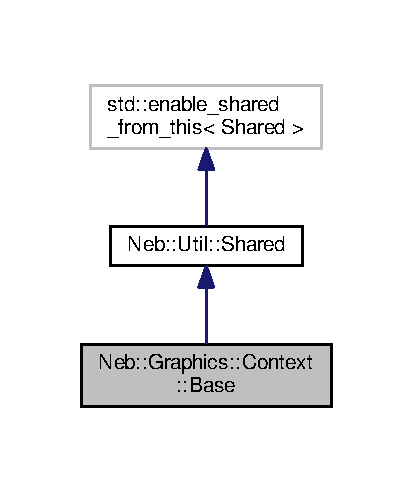
\includegraphics[width=198pt]{classNeb_1_1Graphics_1_1Context_1_1Base__inherit__graph}
\end{center}
\end{figure}


Collaboration diagram for Neb\-:\-:Graphics\-:\-:Context\-:\-:Base\-:
\nopagebreak
\begin{figure}[H]
\begin{center}
\leavevmode
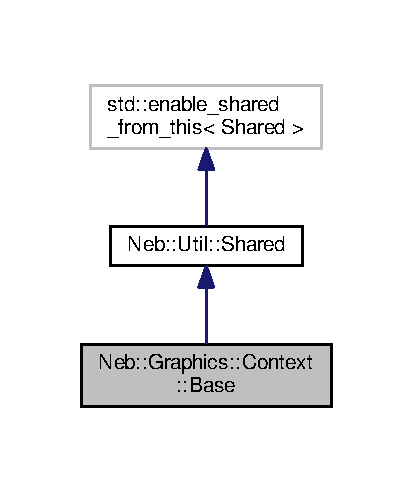
\includegraphics[width=198pt]{classNeb_1_1Graphics_1_1Context_1_1Base__coll__graph}
\end{center}
\end{figure}
\subsection*{Public Member Functions}
\begin{DoxyCompactItemize}
\item 
\hypertarget{classNeb_1_1Graphics_1_1Context_1_1Base_aa95ae98cc0e8e6d41ba4b5f6a6b5daa3}{{\bfseries Base} (Neb\-::\-Graphics\-::\-Context\-::\-Util\-::\-Parent\-\_\-s parent)}\label{classNeb_1_1Graphics_1_1Context_1_1Base_aa95ae98cc0e8e6d41ba4b5f6a6b5daa3}

\item 
\hypertarget{classNeb_1_1Graphics_1_1Context_1_1Base_a20e3b1394b65b6612f164afc2203eb62}{\hyperlink{classNeb_1_1Graphics_1_1Context_1_1Base}{Base} \& {\bfseries operator=} (\hyperlink{classNeb_1_1Graphics_1_1Context_1_1Base}{Base} const \&r)}\label{classNeb_1_1Graphics_1_1Context_1_1Base_a20e3b1394b65b6612f164afc2203eb62}

\item 
\hypertarget{classNeb_1_1Graphics_1_1Context_1_1Base_ae53015c10d1b49295bec4b5a232e00fb}{void {\bfseries init} ()}\label{classNeb_1_1Graphics_1_1Context_1_1Base_ae53015c10d1b49295bec4b5a232e00fb}

\item 
\hypertarget{classNeb_1_1Graphics_1_1Context_1_1Base_ac7029fa00d834d315d5a0e80160fd774}{Neb\-::\-Graphics\-::\-Context\-::\-Util\-::\-Parent\-\_\-s {\bfseries get\-Parent} ()}\label{classNeb_1_1Graphics_1_1Context_1_1Base_ac7029fa00d834d315d5a0e80160fd774}

\item 
\hypertarget{classNeb_1_1Graphics_1_1Context_1_1Base_a37f38f6067db83fcb771dba5df582215}{void {\bfseries resize} (int w, int h)}\label{classNeb_1_1Graphics_1_1Context_1_1Base_a37f38f6067db83fcb771dba5df582215}

\item 
\hypertarget{classNeb_1_1Graphics_1_1Context_1_1Base_a969de7cbec52d89e714dcc56fefacce4}{void {\bfseries render} (double time, Neb\-::\-Graphics\-::\-Window\-::\-Base\-\_\-s window)}\label{classNeb_1_1Graphics_1_1Context_1_1Base_a969de7cbec52d89e714dcc56fefacce4}

\end{DoxyCompactItemize}
\subsection*{Public Attributes}
\begin{DoxyCompactItemize}
\item 
\hypertarget{classNeb_1_1Graphics_1_1Context_1_1Base_a4f3f4b08c7a51f9c03340a0ddaeb7ae6}{Neb\-::\-Scene\-::\-Base\-\_\-w \hyperlink{classNeb_1_1Graphics_1_1Context_1_1Base_a4f3f4b08c7a51f9c03340a0ddaeb7ae6}{scene\-\_\-}}\label{classNeb_1_1Graphics_1_1Context_1_1Base_a4f3f4b08c7a51f9c03340a0ddaeb7ae6}

\begin{DoxyCompactList}\small\item\em scene. weak because scene is owned by app. \end{DoxyCompactList}\item 
\hypertarget{classNeb_1_1Graphics_1_1Context_1_1Base_a0f815690b1cb0a9c84706617298512be}{Neb\-::\-Graphics\-::\-G\-U\-I\-::\-Layout\-::\-Base\-\_\-w \hyperlink{classNeb_1_1Graphics_1_1Context_1_1Base_a0f815690b1cb0a9c84706617298512be}{layout\-\_\-}}\label{classNeb_1_1Graphics_1_1Context_1_1Base_a0f815690b1cb0a9c84706617298512be}

\begin{DoxyCompactList}\small\item\em layout. weak because layout is owned by app. \end{DoxyCompactList}\item 
\hypertarget{classNeb_1_1Graphics_1_1Context_1_1Base_af1062621566e1d6e44eb6de4dcd00e58}{Neb\-::\-Camera\-::\-View\-::\-Base\-\_\-s {\bfseries view\-\_\-}}\label{classNeb_1_1Graphics_1_1Context_1_1Base_af1062621566e1d6e44eb6de4dcd00e58}

\item 
\hypertarget{classNeb_1_1Graphics_1_1Context_1_1Base_a4af90873cf044c83e956776bcc7f262c}{Neb\-::\-Camera\-::\-Projection\-::\-Base\-\_\-s {\bfseries proj\-\_\-}}\label{classNeb_1_1Graphics_1_1Context_1_1Base_a4af90873cf044c83e956776bcc7f262c}

\end{DoxyCompactItemize}


\subsection{Detailed Description}
Renderable. 

\begin{DoxyRefDesc}{Todo}
\item[\hyperlink{todo__todo000010}{Todo}]eventually replace this with \hyperlink{namespaceNeb_1_1Graphics_1_1Context}{Context} and allow multiple Contexts per window and allow scene and layout to have different and overalpping Contexts. \end{DoxyRefDesc}


The documentation for this class was generated from the following file\-:\begin{DoxyCompactItemize}
\item 
src/\-Nebula/\-Graphics/\-Context/Base.\-hh\end{DoxyCompactItemize}

\hypertarget{classNeb_1_1Message_1_1Actor_1_1Base}{\section{Neb\-:\-:Message\-:\-:Actor\-:\-:Base Class Reference}
\label{classNeb_1_1Message_1_1Actor_1_1Base}\index{Neb\-::\-Message\-::\-Actor\-::\-Base@{Neb\-::\-Message\-::\-Actor\-::\-Base}}
}


Inheritance diagram for Neb\-:\-:Message\-:\-:Actor\-:\-:Base\-:
\nopagebreak
\begin{figure}[H]
\begin{center}
\leavevmode
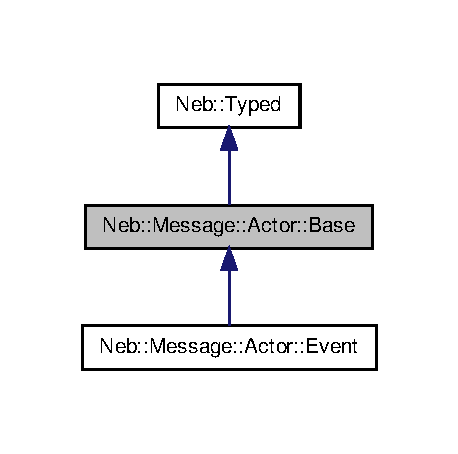
\includegraphics[width=350pt]{classNeb_1_1Message_1_1Actor_1_1Base__inherit__graph}
\end{center}
\end{figure}


Collaboration diagram for Neb\-:\-:Message\-:\-:Actor\-:\-:Base\-:
\nopagebreak
\begin{figure}[H]
\begin{center}
\leavevmode
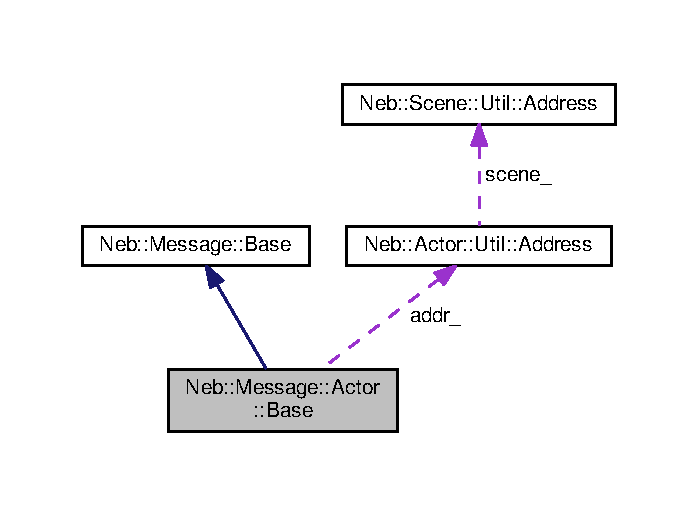
\includegraphics[width=335pt]{classNeb_1_1Message_1_1Actor_1_1Base__coll__graph}
\end{center}
\end{figure}
\subsection*{Public Member Functions}
\begin{DoxyCompactItemize}
\item 
\hypertarget{classNeb_1_1Message_1_1Actor_1_1Base_a961a74203562be229bb3bd1a047dc6d2}{{\footnotesize template$<$class Archive $>$ }\\void {\bfseries serialize} (Archive \&ar, unsigned int const \&version)}\label{classNeb_1_1Message_1_1Actor_1_1Base_a961a74203562be229bb3bd1a047dc6d2}

\item 
\hypertarget{classNeb_1_1Message_1_1Actor_1_1Base_ad8254e0566160c2c27eceae2c63584e9}{virtual void {\bfseries serialize\-Derived} (boost\-::archive\-::polymorphic\-\_\-oarchive \&ar, unsigned int const \&version)=0}\label{classNeb_1_1Message_1_1Actor_1_1Base_ad8254e0566160c2c27eceae2c63584e9}

\item 
\hypertarget{classNeb_1_1Message_1_1Actor_1_1Base_ab34802649e8cd87e5fcdeb9e49a94920}{virtual void {\bfseries serialize\-Derived} (boost\-::archive\-::polymorphic\-\_\-iarchive \&ar, unsigned int const \&version)=0}\label{classNeb_1_1Message_1_1Actor_1_1Base_ab34802649e8cd87e5fcdeb9e49a94920}

\end{DoxyCompactItemize}
\subsection*{Public Attributes}
\begin{DoxyCompactItemize}
\item 
\hypertarget{classNeb_1_1Message_1_1Actor_1_1Base_a2cd0619d9698dea1832247a90979b750}{\hyperlink{classNeb_1_1Actor_1_1Util_1_1Address}{Neb\-::\-Actor\-::\-Util\-::\-Address} {\bfseries addr\-\_\-}}\label{classNeb_1_1Message_1_1Actor_1_1Base_a2cd0619d9698dea1832247a90979b750}

\end{DoxyCompactItemize}
\subsection*{Additional Inherited Members}


The documentation for this class was generated from the following file\-:\begin{DoxyCompactItemize}
\item 
src/\-Nebula/\-Message/\-Actor/Base.\-hh\end{DoxyCompactItemize}

\hypertarget{classNeb_1_1Actor_1_1RigidActor_1_1Base}{\section{\-Neb\-:\-:\-Actor\-:\-:\-Rigid\-Actor\-:\-:\-Base \-Class \-Reference}
\label{classNeb_1_1Actor_1_1RigidActor_1_1Base}\index{\-Neb\-::\-Actor\-::\-Rigid\-Actor\-::\-Base@{\-Neb\-::\-Actor\-::\-Rigid\-Actor\-::\-Base}}
}


\-Inheritance diagram for \-Neb\-:\-:\-Actor\-:\-:\-Rigid\-Actor\-:\-:\-Base\-:\nopagebreak
\begin{figure}[H]
\begin{center}
\leavevmode
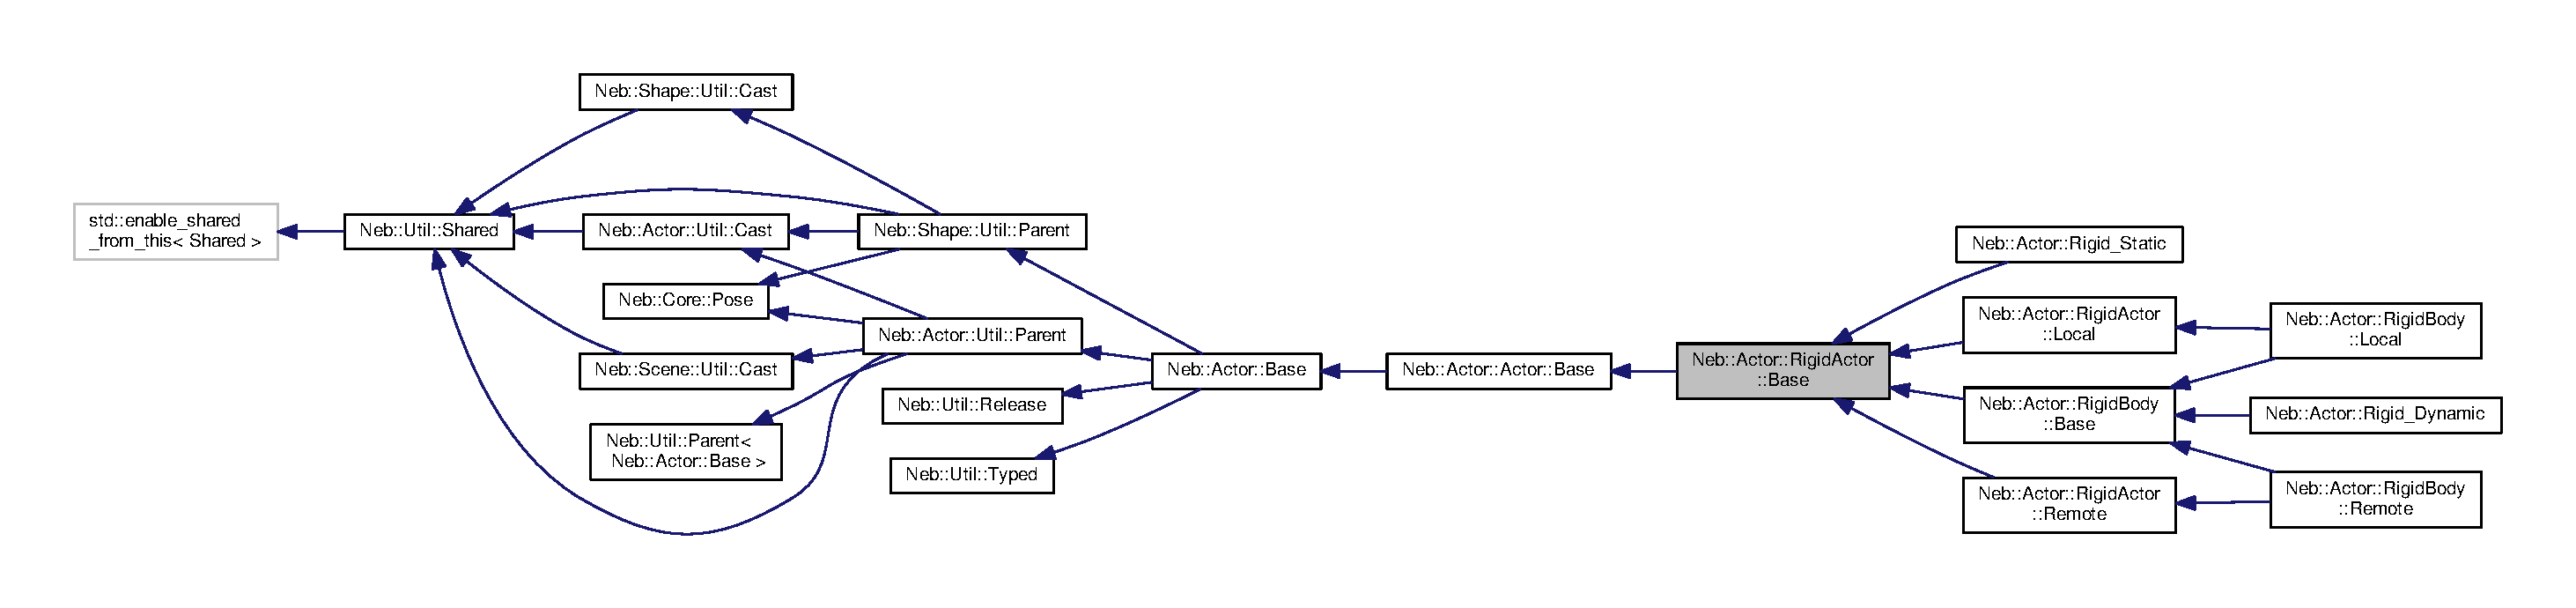
\includegraphics[width=350pt]{classNeb_1_1Actor_1_1RigidActor_1_1Base__inherit__graph}
\end{center}
\end{figure}


\-Collaboration diagram for \-Neb\-:\-:\-Actor\-:\-:\-Rigid\-Actor\-:\-:\-Base\-:\nopagebreak
\begin{figure}[H]
\begin{center}
\leavevmode
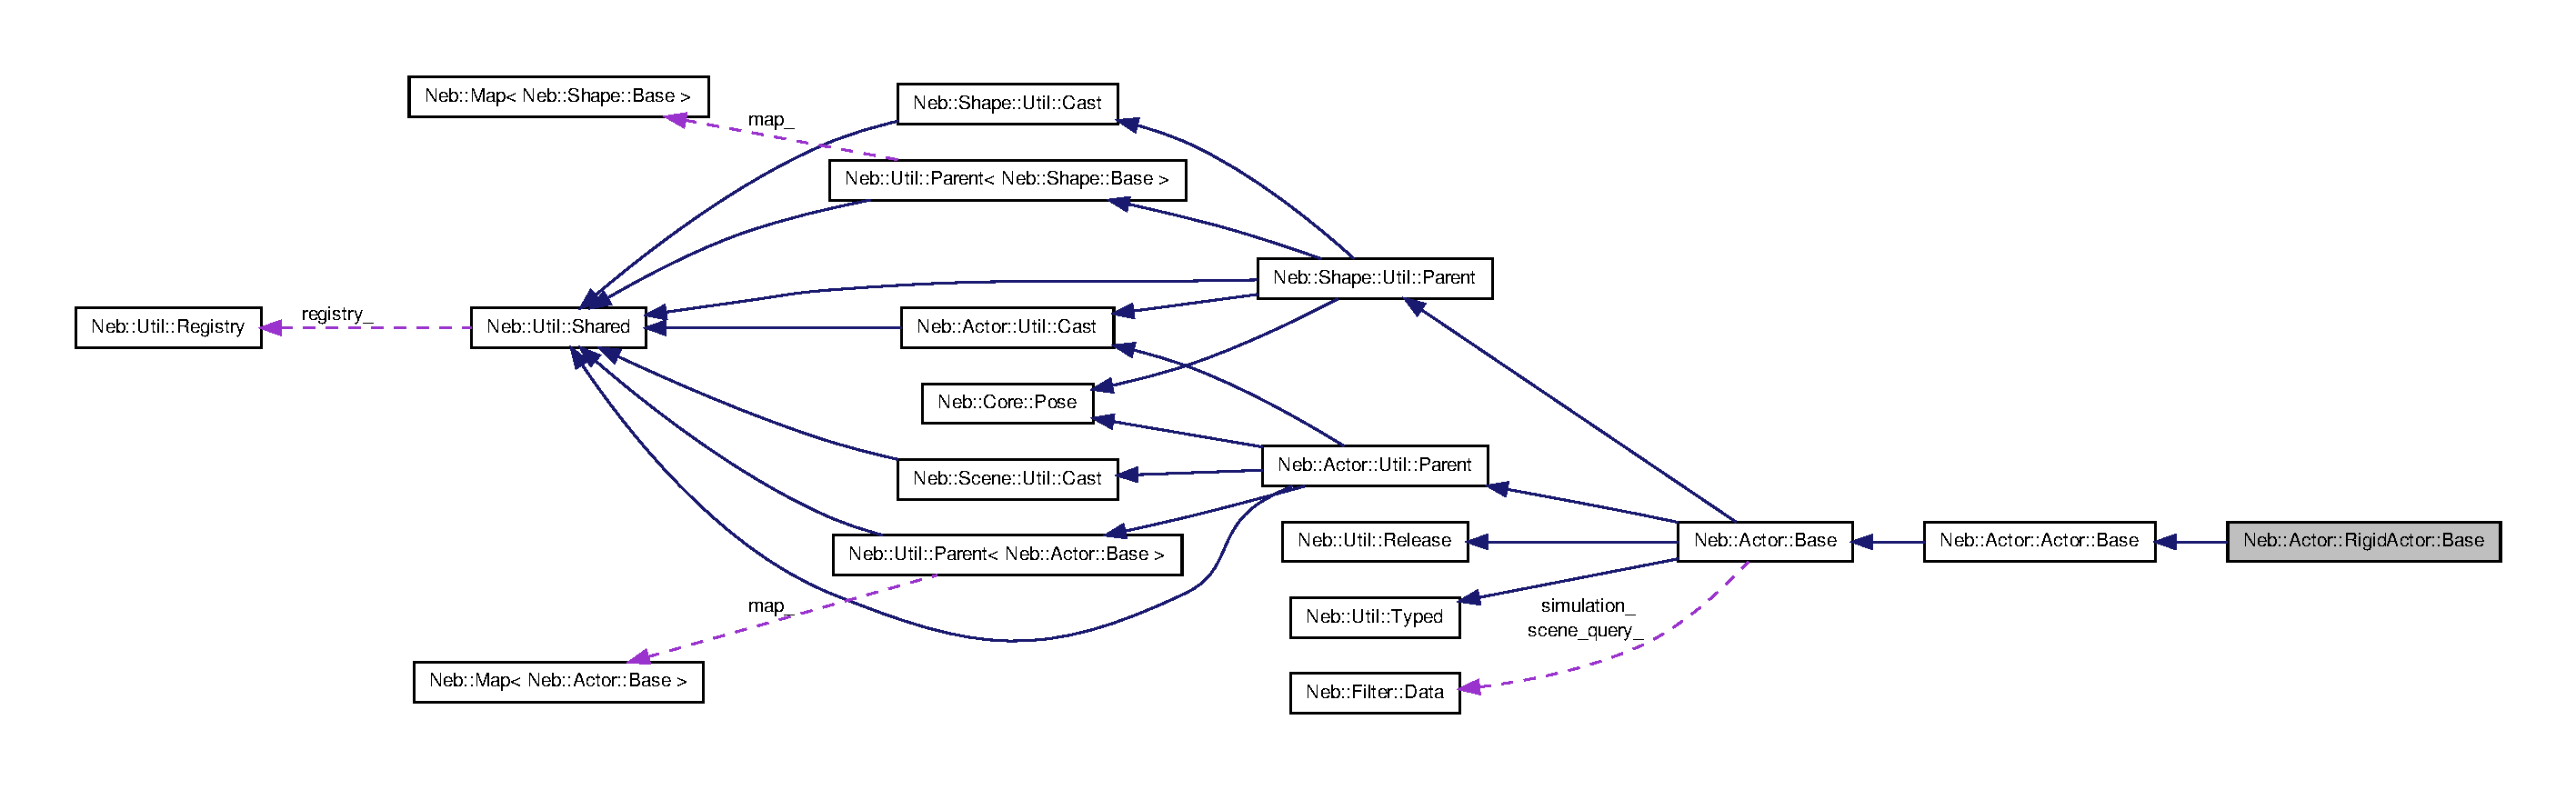
\includegraphics[width=350pt]{classNeb_1_1Actor_1_1RigidActor_1_1Base__coll__graph}
\end{center}
\end{figure}
\subsection*{\-Public \-Member \-Functions}
\begin{DoxyCompactItemize}
\item 
\hypertarget{classNeb_1_1Actor_1_1RigidActor_1_1Base_aa0ba49934f963f62868f795bf30d0094}{{\bfseries \-Base} (\-Neb\-::\-Actor\-::\-Util\-::\-Parent\-\_\-s)}\label{classNeb_1_1Actor_1_1RigidActor_1_1Base_aa0ba49934f963f62868f795bf30d0094}

\item 
\hypertarget{classNeb_1_1Actor_1_1RigidActor_1_1Base_adf9c1fc31512c3b3748342ac9f0ae647}{{\footnotesize template$<$class D , typename... \-Args$>$ }\\void {\bfseries dispatch} (\-Args...\-a)}\label{classNeb_1_1Actor_1_1RigidActor_1_1Base_adf9c1fc31512c3b3748342ac9f0ae647}

\item 
\hypertarget{classNeb_1_1Actor_1_1RigidActor_1_1Base_a766bc8b5e81030cad05207e9ed76ba94}{virtual void {\bfseries init} ()}\label{classNeb_1_1Actor_1_1RigidActor_1_1Base_a766bc8b5e81030cad05207e9ed76ba94}

\item 
\hypertarget{classNeb_1_1Actor_1_1RigidActor_1_1Base_a33114287de0d373ceca81a52c41745ad}{virtual void {\bfseries step} (double const \&time, double const \&dt)}\label{classNeb_1_1Actor_1_1RigidActor_1_1Base_a33114287de0d373ceca81a52c41745ad}

\item 
\hypertarget{classNeb_1_1Actor_1_1RigidActor_1_1Base_accf86e508f0ab034bd212b1264644a4c}{virtual void {\bfseries setup\-Filtering} ()}\label{classNeb_1_1Actor_1_1RigidActor_1_1Base_accf86e508f0ab034bd212b1264644a4c}

\item 
\hypertarget{classNeb_1_1Actor_1_1RigidActor_1_1Base_a7fe627181ce217ec0dfd5eb23b410c49}{virtual \-Neb\-::\-Actor\-::\-Base\-\_\-s {\bfseries get\-\_\-projectile} ()=0}\label{classNeb_1_1Actor_1_1RigidActor_1_1Base_a7fe627181ce217ec0dfd5eb23b410c49}

\item 
\hypertarget{classNeb_1_1Actor_1_1RigidActor_1_1Base_ac7662178d8468d3d80fe1074f3e03277}{virtual void {\bfseries create\-\_\-physics} ()=0}\label{classNeb_1_1Actor_1_1RigidActor_1_1Base_ac7662178d8468d3d80fe1074f3e03277}

\item 
\hypertarget{classNeb_1_1Actor_1_1RigidActor_1_1Base_aff211aa28ad50ac3f141bfbde642d738}{virtual void {\bfseries init\-\_\-physics} ()=0}\label{classNeb_1_1Actor_1_1RigidActor_1_1Base_aff211aa28ad50ac3f141bfbde642d738}

\end{DoxyCompactItemize}


\-The documentation for this class was generated from the following files\-:\begin{DoxyCompactItemize}
\item 
src/\-Nebula/\-Actor/\-Rigid\-Actor/\-Base.\-hh\item 
src/\-Nebula/\-Actor/\-Rigid\-Actor/\-Base.\-cc\end{DoxyCompactItemize}

\hypertarget{classNeb_1_1glsl_1_1Uniform_1_1Scalar_1_1Base}{\section{\-Neb\-:\-:glsl\-:\-:\-Uniform\-:\-:\-Scalar\-:\-:\-Base \-Class \-Reference}
\label{classNeb_1_1glsl_1_1Uniform_1_1Scalar_1_1Base}\index{\-Neb\-::glsl\-::\-Uniform\-::\-Scalar\-::\-Base@{\-Neb\-::glsl\-::\-Uniform\-::\-Scalar\-::\-Base}}
}


\-Base  




{\ttfamily \#include $<$uniform.\-hh$>$}



\-Inheritance diagram for \-Neb\-:\-:glsl\-:\-:\-Uniform\-:\-:\-Scalar\-:\-:\-Base\-:\nopagebreak
\begin{figure}[H]
\begin{center}
\leavevmode
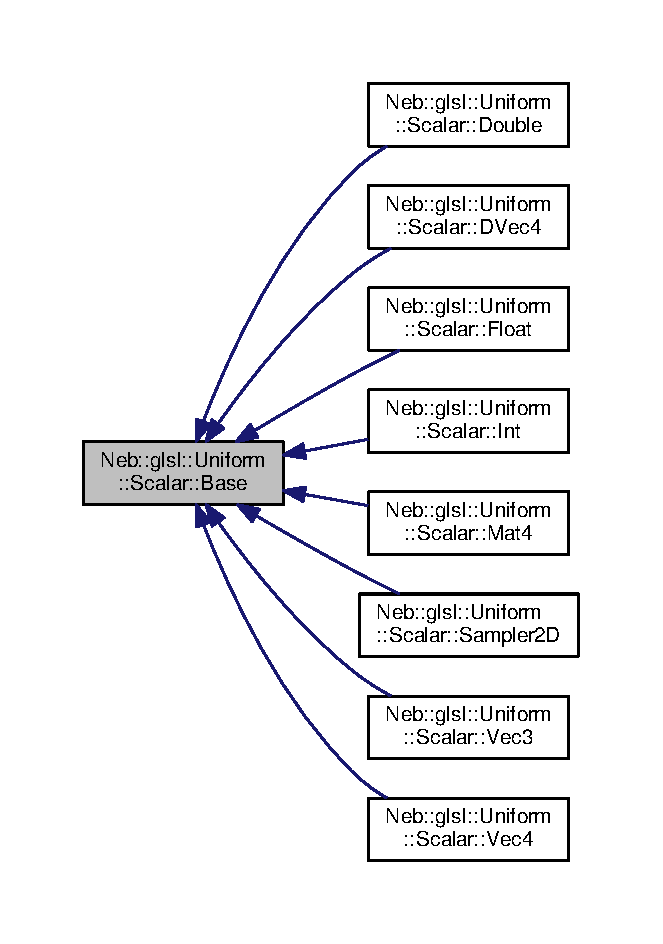
\includegraphics[width=350pt]{classNeb_1_1glsl_1_1Uniform_1_1Scalar_1_1Base__inherit__graph}
\end{center}
\end{figure}
\subsection*{\-Public \-Member \-Functions}
\begin{DoxyCompactItemize}
\item 
\hypertarget{classNeb_1_1glsl_1_1Uniform_1_1Scalar_1_1Base_a641383ec850d2d546d36e3b1b876aaec}{{\bfseries \-Base} (std\-::string)}\label{classNeb_1_1glsl_1_1Uniform_1_1Scalar_1_1Base_a641383ec850d2d546d36e3b1b876aaec}

\item 
\hypertarget{classNeb_1_1glsl_1_1Uniform_1_1Scalar_1_1Base_a33dcd3c2259cbb51de388b7433bec7ea}{void {\bfseries locate} (std\-::shared\-\_\-ptr$<$ \hyperlink{classNeb_1_1glsl_1_1program}{program} $>$)}\label{classNeb_1_1glsl_1_1Uniform_1_1Scalar_1_1Base_a33dcd3c2259cbb51de388b7433bec7ea}

\end{DoxyCompactItemize}
\begin{Indent}{\bf \-Load}\par
\begin{DoxyCompactItemize}
\item 
\hypertarget{classNeb_1_1glsl_1_1Uniform_1_1Scalar_1_1Base_ace5fa46d19dbcaeb70a870739274f6e8}{virtual void {\bfseries load} (physx\-::\-Px\-Vec3 const \&)}\label{classNeb_1_1glsl_1_1Uniform_1_1Scalar_1_1Base_ace5fa46d19dbcaeb70a870739274f6e8}

\item 
\hypertarget{classNeb_1_1glsl_1_1Uniform_1_1Scalar_1_1Base_a4ce7aa148065323048dddbc2b080f6af}{virtual void {\bfseries load} (physx\-::\-Px\-Vec4 const \&)}\label{classNeb_1_1glsl_1_1Uniform_1_1Scalar_1_1Base_a4ce7aa148065323048dddbc2b080f6af}

\item 
\hypertarget{classNeb_1_1glsl_1_1Uniform_1_1Scalar_1_1Base_a157ee5aaa15e8bbd2da6068de06982e6}{virtual void {\bfseries load} (physx\-::\-Px\-Mat44 const \&)}\label{classNeb_1_1glsl_1_1Uniform_1_1Scalar_1_1Base_a157ee5aaa15e8bbd2da6068de06982e6}

\item 
\hypertarget{classNeb_1_1glsl_1_1Uniform_1_1Scalar_1_1Base_a8030d1d34cf561d295de77977456aa03}{virtual void {\bfseries load} (int)}\label{classNeb_1_1glsl_1_1Uniform_1_1Scalar_1_1Base_a8030d1d34cf561d295de77977456aa03}

\item 
\hypertarget{classNeb_1_1glsl_1_1Uniform_1_1Scalar_1_1Base_a8433a02ab6d2f7630b11ca43286699e6}{virtual void {\bfseries load} (float $\ast$)}\label{classNeb_1_1glsl_1_1Uniform_1_1Scalar_1_1Base_a8433a02ab6d2f7630b11ca43286699e6}

\item 
\hypertarget{classNeb_1_1glsl_1_1Uniform_1_1Scalar_1_1Base_aaf47edc4ad36bdd9b3ffbc38c8c3f22d}{virtual void {\bfseries load} (double $\ast$)}\label{classNeb_1_1glsl_1_1Uniform_1_1Scalar_1_1Base_aaf47edc4ad36bdd9b3ffbc38c8c3f22d}

\item 
\hypertarget{classNeb_1_1glsl_1_1Uniform_1_1Scalar_1_1Base_aa00b3fcd3a40fa1634b00cfbc114f6cb}{virtual void {\bfseries load} (float)}\label{classNeb_1_1glsl_1_1Uniform_1_1Scalar_1_1Base_aa00b3fcd3a40fa1634b00cfbc114f6cb}

\item 
\hypertarget{classNeb_1_1glsl_1_1Uniform_1_1Scalar_1_1Base_af41da8bb1fee6323ad56aa45fe303e32}{virtual void {\bfseries load} (double)}\label{classNeb_1_1glsl_1_1Uniform_1_1Scalar_1_1Base_af41da8bb1fee6323ad56aa45fe303e32}

\end{DoxyCompactItemize}
\end{Indent}
\subsection*{\-Protected \-Attributes}
\begin{DoxyCompactItemize}
\item 
\hypertarget{classNeb_1_1glsl_1_1Uniform_1_1Scalar_1_1Base_af4f8e92fee448c545de153937a419abe}{std\-::string {\bfseries name\-\_\-}}\label{classNeb_1_1glsl_1_1Uniform_1_1Scalar_1_1Base_af4f8e92fee448c545de153937a419abe}

\item 
\hypertarget{classNeb_1_1glsl_1_1Uniform_1_1Scalar_1_1Base_ac57d0525c2866193e87adde9b8ef36fe}{\-G\-Lint {\bfseries o\-\_\-}}\label{classNeb_1_1glsl_1_1Uniform_1_1Scalar_1_1Base_ac57d0525c2866193e87adde9b8ef36fe}

\end{DoxyCompactItemize}


\subsection{\-Detailed \-Description}
\-Base 

base class for scalar \-G\-L\-S\-L uniform 

\-The documentation for this class was generated from the following files\-:\begin{DoxyCompactItemize}
\item 
src/\-Nebula/\-Graphics/glsl/\-Uniform/uniform.\-hh\item 
src/\-Nebula/\-Graphics/glsl/\-Uniform/\-Scalar.\-cc\end{DoxyCompactItemize}

\hypertarget{classNeb_1_1Message_1_1Base}{\section{\-Neb\-:\-:\-Message\-:\-:\-Base \-Class \-Reference}
\label{classNeb_1_1Message_1_1Base}\index{\-Neb\-::\-Message\-::\-Base@{\-Neb\-::\-Message\-::\-Base}}
}


\-The documentation for this class was generated from the following file\-:\begin{DoxyCompactItemize}
\item 
src/gru/\-Message/\-Base.\-hpp\end{DoxyCompactItemize}

\hypertarget{classNeb_1_1App_1_1BaseFactory}{\section{\-Neb\-:\-:\-App\-:\-:\-Base\-Factory \-Class \-Reference}
\label{classNeb_1_1App_1_1BaseFactory}\index{\-Neb\-::\-App\-::\-Base\-Factory@{\-Neb\-::\-App\-::\-Base\-Factory}}
}


\-Inheritance diagram for \-Neb\-:\-:\-App\-:\-:\-Base\-Factory\-:\nopagebreak
\begin{figure}[H]
\begin{center}
\leavevmode
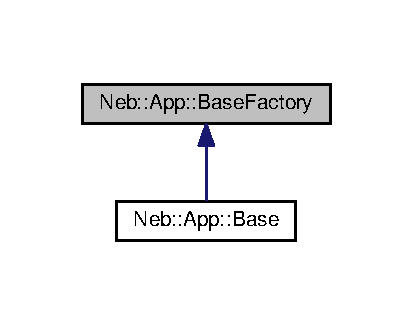
\includegraphics[width=198pt]{classNeb_1_1App_1_1BaseFactory__inherit__graph}
\end{center}
\end{figure}
\subsection*{\-Public \-Types}
\begin{DoxyCompactItemize}
\item 
\hypertarget{classNeb_1_1App_1_1BaseFactory_a7900d6b4a474fc9d95b62c23306af2fa}{typedef pointer$<$ \hyperlink{classNeb_1_1Factory}{\-Neb\-::\-Factory}\*
$<$ \hyperlink{classNeb_1_1Graphics_1_1GUI_1_1Object_1_1Base}{\-Neb\-::\-Graphics\-::\-G\-U\-I\-::\-Object\-::\-Base} $>$ $>$ {\bfseries \-G\-U\-I\-\_\-\-Object}}\label{classNeb_1_1App_1_1BaseFactory_a7900d6b4a474fc9d95b62c23306af2fa}

\item 
\hypertarget{classNeb_1_1App_1_1BaseFactory_adb13eef681dd64d83bd14d29adcab67c}{typedef pointer$<$ \hyperlink{classNeb_1_1Factory}{\-Neb\-::\-Factory}\*
$<$ \hyperlink{classNeb_1_1Actor_1_1Base}{\-Neb\-::\-Actor\-::\-Base} $>$ $>$ {\bfseries \-Factory\-\_\-\-Actor\-\_\-\-Base}}\label{classNeb_1_1App_1_1BaseFactory_adb13eef681dd64d83bd14d29adcab67c}

\item 
\hypertarget{classNeb_1_1App_1_1BaseFactory_ad68d4c2c4834639335124a003e34b37c}{typedef pointer$<$ \hyperlink{classNeb_1_1Factory}{\-Neb\-::\-Factory}\*
$<$ \hyperlink{classNeb_1_1Shape_1_1Base}{\-Neb\-::\-Shape\-::\-Base} $>$ $>$ {\bfseries \-Shape\-\_\-\-Base}}\label{classNeb_1_1App_1_1BaseFactory_ad68d4c2c4834639335124a003e34b37c}

\item 
\hypertarget{classNeb_1_1App_1_1BaseFactory_ad77d1d1ba2072913470814fa00f7639c}{typedef pointer$<$ \hyperlink{classNeb_1_1Factory}{\-Neb\-::\-Factory}\*
$<$ \-Neb\-::\-Light\-::light $>$ $>$ {\bfseries \-Light\-\_\-\-Base}}\label{classNeb_1_1App_1_1BaseFactory_ad77d1d1ba2072913470814fa00f7639c}

\item 
\hypertarget{classNeb_1_1App_1_1BaseFactory_a2e1133c47fbc9aec044fe8b98ea33d21}{typedef pointer$<$ \hyperlink{classNeb_1_1Factory}{\-Neb\-::\-Factory}\*
$<$ \hyperlink{classNeb_1_1Graphics_1_1Window_1_1Base}{\-Neb\-::\-Graphics\-::\-Window\-::\-Base} $>$ $>$ {\bfseries \-Window\-\_\-\-Base}}\label{classNeb_1_1App_1_1BaseFactory_a2e1133c47fbc9aec044fe8b98ea33d21}

\item 
\hypertarget{classNeb_1_1App_1_1BaseFactory_a4d57ec8c91ce0c02f40c5a9ecb0bae6f}{typedef pointer$<$ \hyperlink{classNeb_1_1Factory}{\-Neb\-::\-Factory}\*
$<$ \hyperlink{classNeb_1_1Scene_1_1Base}{\-Neb\-::\-Scene\-::\-Base} $>$ $>$ {\bfseries \-Scene\-\_\-\-Base}}\label{classNeb_1_1App_1_1BaseFactory_a4d57ec8c91ce0c02f40c5a9ecb0bae6f}

\end{DoxyCompactItemize}
\subsection*{\-Public \-Member \-Functions}
\begin{DoxyCompactItemize}
\item 
\hypertarget{classNeb_1_1App_1_1BaseFactory_a76250fbb3f8a06b4097b48fcea26884b}{{\footnotesize template$<$class T $>$ }\\std\-::shared\-\_\-ptr$<$ \hyperlink{classNeb_1_1Factory}{\-Neb\-::\-Factory}\*
$<$ \-T $>$ $>$ {\bfseries get\-Factory\-Default} ()}\label{classNeb_1_1App_1_1BaseFactory_a76250fbb3f8a06b4097b48fcea26884b}

\end{DoxyCompactItemize}
\subsection*{\-Static \-Public \-Member \-Functions}
\begin{DoxyCompactItemize}
\item 
\hypertarget{classNeb_1_1App_1_1BaseFactory_a8abc6f8df757702cb7586e22a59cc70d}{static void {\bfseries init} ()}\label{classNeb_1_1App_1_1BaseFactory_a8abc6f8df757702cb7586e22a59cc70d}

\item 
\hypertarget{classNeb_1_1App_1_1BaseFactory_a3b8dc92ce1506c8f4bd046aed4b769c6}{static \-Base\-Factory\-\_\-s {\bfseries global} ()}\label{classNeb_1_1App_1_1BaseFactory_a3b8dc92ce1506c8f4bd046aed4b769c6}

\end{DoxyCompactItemize}
\subsection*{\-Public \-Attributes}
\begin{DoxyCompactItemize}
\item 
\hypertarget{classNeb_1_1App_1_1BaseFactory_a90c445809d58f4a52188a16832438702}{\begin{tabbing}
xx\=xx\=xx\=xx\=xx\=xx\=xx\=xx\=xx\=\kill
struct \{\\
\>GUI\_Object {\bfseries gui\_object\_}\\
\>Factory\_Actor\_Base {\bfseries actor\_base\_}\\
\>Shape\_Base {\bfseries shape\_base\_}\\
\>Light\_Base {\bfseries light\_base\_}\\
\>Window\_Base {\bfseries window\_base\_}\\
\>Scene\_Base {\bfseries scene\_base\_}\\
\} \hyperlink{classNeb_1_1App_1_1BaseFactory_a90c445809d58f4a52188a16832438702}{factories\_}}\label{classNeb_1_1App_1_1BaseFactory_a90c445809d58f4a52188a16832438702}
\\

\end{tabbing}\begin{DoxyCompactList}\small\item\em \-Factories. \end{DoxyCompactList}\end{DoxyCompactItemize}
\subsection*{\-Static \-Protected \-Attributes}
\begin{DoxyCompactItemize}
\item 
static \-Neb\-::\-App\-::\-Base\-Factory\-\_\-s \hyperlink{classNeb_1_1App_1_1BaseFactory_a2add590edaa414b5346b67af7ce9d344}{g\-\_\-app\-\_\-}
\end{DoxyCompactItemize}


\subsection{\-Member \-Data \-Documentation}
\hypertarget{classNeb_1_1App_1_1BaseFactory_a2add590edaa414b5346b67af7ce9d344}{\index{\-Neb\-::\-App\-::\-Base\-Factory@{\-Neb\-::\-App\-::\-Base\-Factory}!g\-\_\-app\-\_\-@{g\-\_\-app\-\_\-}}
\index{g\-\_\-app\-\_\-@{g\-\_\-app\-\_\-}!Neb::App::BaseFactory@{\-Neb\-::\-App\-::\-Base\-Factory}}
\subsubsection[{g\-\_\-app\-\_\-}]{\setlength{\rightskip}{0pt plus 5cm}std\-::shared\-\_\-ptr$<$ {\bf \-Neb\-::\-App\-::\-Base\-Factory} $>$ {\bf \-Neb\-::\-App\-::\-Base\-Factory\-::g\-\_\-app\-\_\-}\hspace{0.3cm}{\ttfamily  \mbox{[}static, protected\mbox{]}}}}\label{classNeb_1_1App_1_1BaseFactory_a2add590edaa414b5346b67af7ce9d344}
brief global app object 

\-The documentation for this class was generated from the following files\-:\begin{DoxyCompactItemize}
\item 
src/\-Nebula/\-App/\-Base\-Factory.\-hh\item 
src/\-Nebula/\-App/\-Base\-Factory.\-cc\end{DoxyCompactItemize}

\hypertarget{classNeb_1_1Shape_1_1Box_1_1Box}{\section{\-Neb\-:\-:\-Shape\-:\-:\-Box\-:\-:\-Box \-Class \-Reference}
\label{classNeb_1_1Shape_1_1Box_1_1Box}\index{\-Neb\-::\-Shape\-::\-Box\-::\-Box@{\-Neb\-::\-Shape\-::\-Box\-::\-Box}}
}


\-Inheritance diagram for \-Neb\-:\-:\-Shape\-:\-:\-Box\-:\-:\-Box\-:\nopagebreak
\begin{figure}[H]
\begin{center}
\leavevmode
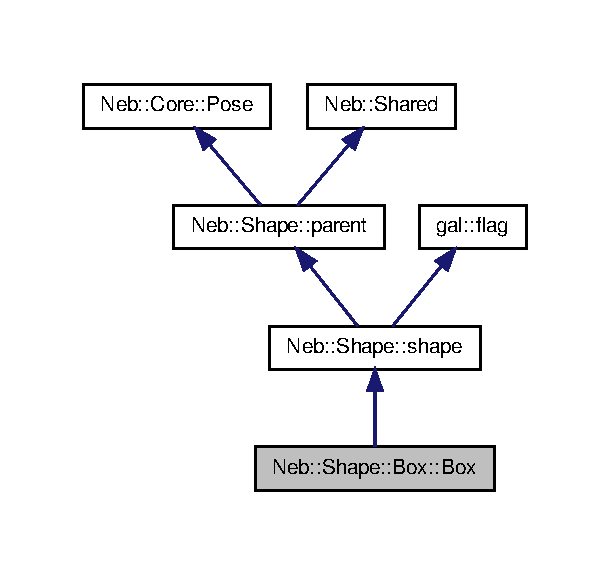
\includegraphics[width=292pt]{classNeb_1_1Shape_1_1Box_1_1Box__inherit__graph}
\end{center}
\end{figure}


\-Collaboration diagram for \-Neb\-:\-:\-Shape\-:\-:\-Box\-:\-:\-Box\-:\nopagebreak
\begin{figure}[H]
\begin{center}
\leavevmode
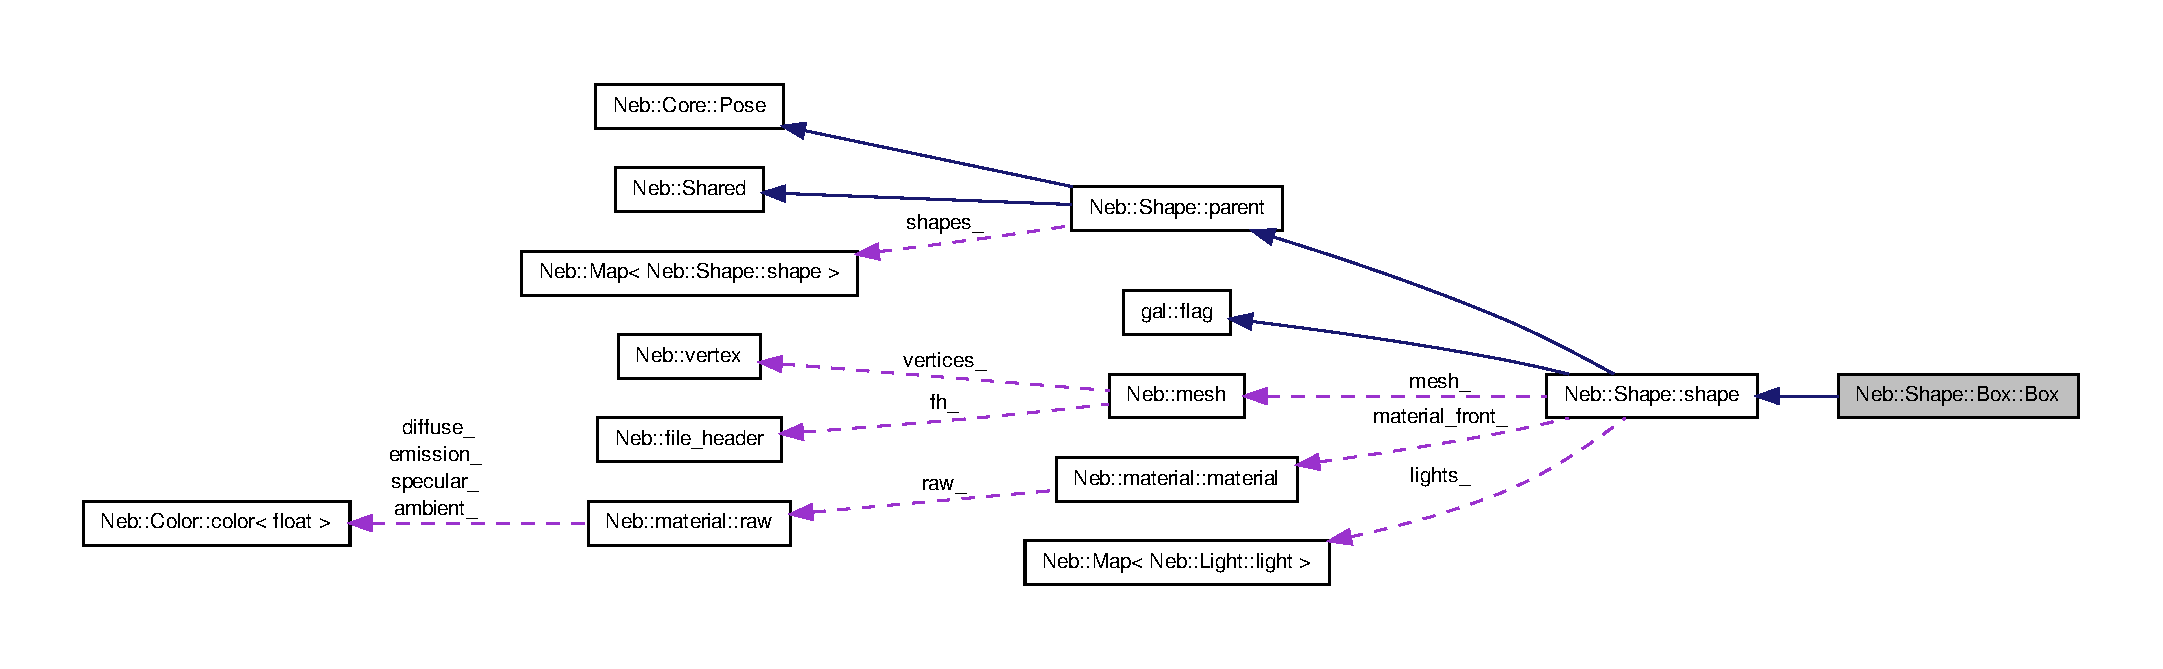
\includegraphics[width=350pt]{classNeb_1_1Shape_1_1Box_1_1Box__coll__graph}
\end{center}
\end{figure}
\subsection*{\-Private \-Member \-Functions}
\begin{DoxyCompactItemize}
\item 
\hypertarget{classNeb_1_1Shape_1_1Box_1_1Box_a03026c27dd9898c1b1a4ac7103cd834d}{virtual void {\bfseries create\-Mesh} ()}\label{classNeb_1_1Shape_1_1Box_1_1Box_a03026c27dd9898c1b1a4ac7103cd834d}

\end{DoxyCompactItemize}


\-The documentation for this class was generated from the following files\-:\begin{DoxyCompactItemize}
\item 
src/\-Nebula/shape/shape.\-hpp\item 
src/\-Nebula/shape/shape.\-cpp\end{DoxyCompactItemize}

\hypertarget{classglutpp_1_1buffer}{\section{glutpp\-:\-:buffer Class Reference}
\label{classglutpp_1_1buffer}\index{glutpp\-::buffer@{glutpp\-::buffer}}
}
\subsection*{Public Member Functions}
\begin{DoxyCompactItemize}
\item 
\hypertarget{classglutpp_1_1buffer_a557629990348485f76e992293cfdb636}{void {\bfseries init} ()}\label{classglutpp_1_1buffer_a557629990348485f76e992293cfdb636}

\item 
\hypertarget{classglutpp_1_1buffer_a37d4b5aac0052a9724b94784205945e7}{void {\bfseries bind} ()}\label{classglutpp_1_1buffer_a37d4b5aac0052a9724b94784205945e7}

\item 
\hypertarget{classglutpp_1_1buffer_af93df84319c7d459b77c4c0c5e515119}{void {\bfseries unbind} ()}\label{classglutpp_1_1buffer_af93df84319c7d459b77c4c0c5e515119}

\end{DoxyCompactItemize}
\subsection*{Public Attributes}
\begin{DoxyCompactItemize}
\item 
\hypertarget{classglutpp_1_1buffer_a45bc4e78c108b155f79e81901b7faba1}{G\-Luint {\bfseries o\-\_\-}}\label{classglutpp_1_1buffer_a45bc4e78c108b155f79e81901b7faba1}

\end{DoxyCompactItemize}


The documentation for this class was generated from the following file\-:\begin{DoxyCompactItemize}
\item 
src/\-Nebula/buffer.\-hh\end{DoxyCompactItemize}

\hypertarget{classNeb_1_1Shape_1_1buffer}{\section{\-Neb\-:\-:\-Shape\-:\-:buffer \-Class \-Reference}
\label{classNeb_1_1Shape_1_1buffer}\index{\-Neb\-::\-Shape\-::buffer@{\-Neb\-::\-Shape\-::buffer}}
}
\subsection*{\-Public \-Attributes}
\begin{DoxyCompactItemize}
\item 
\hypertarget{classNeb_1_1Shape_1_1buffer_a7b21c1e6b3948f4b268185d3f346ab51}{\-G\-Luint {\bfseries vbo\-\_\-}}\label{classNeb_1_1Shape_1_1buffer_a7b21c1e6b3948f4b268185d3f346ab51}

\item 
\hypertarget{classNeb_1_1Shape_1_1buffer_a67e7b3ef9ac4b38e13cb59c54aa7dcd8}{\-G\-Luint {\bfseries indices\-\_\-}}\label{classNeb_1_1Shape_1_1buffer_a67e7b3ef9ac4b38e13cb59c54aa7dcd8}

\item 
\hypertarget{classNeb_1_1Shape_1_1buffer_a70b7b61e93fd8f7ffaf9fadf405526fa}{\begin{tabbing}
xx\=xx\=xx\=xx\=xx\=xx\=xx\=xx\=xx\=\kill
struct \{\\
\>std::shared\_ptr$<$ \hyperlink{classNeb_1_1texture}{Neb::texture} $>$ {\bfseries image\_}\\
\} {\bfseries texture\_}}\label{classNeb_1_1Shape_1_1buffer_a70b7b61e93fd8f7ffaf9fadf405526fa}
\\

\end{tabbing}\end{DoxyCompactItemize}


\-The documentation for this class was generated from the following file\-:\begin{DoxyCompactItemize}
\item 
src/\-Nebula/\-Shape/\-Base.\-hh\end{DoxyCompactItemize}

\hypertarget{classneb_1_1camera_1_1camera}{\section{neb\-:\-:camera\-:\-:camera \-Class \-Reference}
\label{classneb_1_1camera_1_1camera}\index{neb\-::camera\-::camera@{neb\-::camera\-::camera}}
}
\subsection*{\-Public \-Types}
\begin{DoxyCompactItemize}
\item 
enum {\bfseries flag} \{ {\bfseries \-N\-O\-R\-T\-H} =  1 $<$$<$ 0, 
{\bfseries \-S\-O\-U\-T\-H} =  1 $<$$<$ 1, 
{\bfseries \-E\-A\-S\-T} =  1 $<$$<$ 2, 
{\bfseries \-W\-E\-S\-T} =  1 $<$$<$ 3
 \}
\end{DoxyCompactItemize}
\subsection*{\-Public \-Member \-Functions}
\begin{DoxyCompactItemize}
\item 
\hypertarget{classneb_1_1camera_1_1camera_a218cc11e01e31704f8da897c945d0e3f}{void {\bfseries \-Connect} ()}\label{classneb_1_1camera_1_1camera_a218cc11e01e31704f8da897c945d0e3f}

\item 
\hypertarget{classneb_1_1camera_1_1camera_a1648a17ee1479e429d6f642aa57245e9}{void {\bfseries delete\-\_\-scene} ()}\label{classneb_1_1camera_1_1camera_a1648a17ee1479e429d6f642aa57245e9}

\item 
\hypertarget{classneb_1_1camera_1_1camera_a1e6c6198d5b7bdd988b50a2b46b70385}{void {\bfseries \-Display} ()}\label{classneb_1_1camera_1_1camera_a1e6c6198d5b7bdd988b50a2b46b70385}

\item 
\hypertarget{classneb_1_1camera_1_1camera_a2c81ea18393516ad0e70316be6b17daf}{void {\bfseries \-Look} ()}\label{classneb_1_1camera_1_1camera_a2c81ea18393516ad0e70316be6b17daf}

\item 
\hypertarget{classneb_1_1camera_1_1camera_a8ce61b5956d05f57c23a9af81a8a3460}{physx\-::\-Px\-Vec3 {\bfseries \-Move} ()}\label{classneb_1_1camera_1_1camera_a8ce61b5956d05f57c23a9af81a8a3460}

\item 
\hypertarget{classneb_1_1camera_1_1camera_a962445a098d9fc97d17e62238b598fc1}{void {\bfseries \-Step} (float)}\label{classneb_1_1camera_1_1camera_a962445a098d9fc97d17e62238b598fc1}

\item 
\hypertarget{classneb_1_1camera_1_1camera_ae58f39bface93cd1949dd99ff6a72e00}{virtual math\-::mat44 {\bfseries supply} ()}\label{classneb_1_1camera_1_1camera_ae58f39bface93cd1949dd99ff6a72e00}

\item 
\hypertarget{classneb_1_1camera_1_1camera_a2afc49581aedd2419fbc15ff8b365a6f}{int {\bfseries \-First\-Order\-Delta\-Pitch\-Rel} (int)}\label{classneb_1_1camera_1_1camera_a2afc49581aedd2419fbc15ff8b365a6f}

\item 
\hypertarget{classneb_1_1camera_1_1camera_a1fd9fdc99f7de5a8a5fe418abb00e723}{int {\bfseries \-First\-Order\-Delta\-Yaw\-Rel} (int)}\label{classneb_1_1camera_1_1camera_a1fd9fdc99f7de5a8a5fe418abb00e723}

\item 
\hypertarget{classneb_1_1camera_1_1camera_ac0cb12fe6c353757c7960889a01bfd43}{int {\bfseries \-First\-Order\-Delta\-Pitch\-Abs} (float)}\label{classneb_1_1camera_1_1camera_ac0cb12fe6c353757c7960889a01bfd43}

\item 
\hypertarget{classneb_1_1camera_1_1camera_ac6b6e2036f41baa73094872831bab7ad}{int {\bfseries \-First\-Order\-Delta\-Yaw\-Abs} (float)}\label{classneb_1_1camera_1_1camera_ac6b6e2036f41baa73094872831bab7ad}

\item 
\hypertarget{classneb_1_1camera_1_1camera_a739b1a922fcd8341de5b05db808e1985}{int {\bfseries \-Handle\-Abs\-North} (float)}\label{classneb_1_1camera_1_1camera_a739b1a922fcd8341de5b05db808e1985}

\item 
\hypertarget{classneb_1_1camera_1_1camera_aee1530ddb5c9fcd5f9bafd416a9dece8}{int {\bfseries \-Handle\-Abs\-East} (float)}\label{classneb_1_1camera_1_1camera_aee1530ddb5c9fcd5f9bafd416a9dece8}

\item 
\hypertarget{classneb_1_1camera_1_1camera_a4c2b9b9a1f2dab505c592a67beaea6c3}{int {\bfseries \-Handle\-Key\-North} (int)}\label{classneb_1_1camera_1_1camera_a4c2b9b9a1f2dab505c592a67beaea6c3}

\item 
\hypertarget{classneb_1_1camera_1_1camera_ad61600febe8c5a8c9354537d35c97db7}{int {\bfseries \-Handle\-Key\-South} (int)}\label{classneb_1_1camera_1_1camera_ad61600febe8c5a8c9354537d35c97db7}

\item 
\hypertarget{classneb_1_1camera_1_1camera_ad7ef282fa6376a88230adddca92e4476}{int {\bfseries \-Handle\-Key\-East} (int)}\label{classneb_1_1camera_1_1camera_ad7ef282fa6376a88230adddca92e4476}

\item 
\hypertarget{classneb_1_1camera_1_1camera_a9dd8431138fa176fa0d9e47217857f49}{int {\bfseries \-Handle\-Key\-West} (int)}\label{classneb_1_1camera_1_1camera_a9dd8431138fa176fa0d9e47217857f49}

\item 
\hypertarget{classneb_1_1camera_1_1camera_a29fcbce1b15bb165e5133b403bb7eee6}{int {\bfseries handle\-\_\-delete\-\_\-scene} (int)}\label{classneb_1_1camera_1_1camera_a29fcbce1b15bb165e5133b403bb7eee6}

\end{DoxyCompactItemize}
\subsection*{\-Public \-Attributes}
\begin{DoxyCompactItemize}
\item 
\hypertarget{classneb_1_1camera_1_1camera_a9e2f60405bd7ac4f545196a16f49248f}{unsigned int {\bfseries flag\-\_\-}}\label{classneb_1_1camera_1_1camera_a9e2f60405bd7ac4f545196a16f49248f}

\item 
\hypertarget{classneb_1_1camera_1_1camera_a6961799cec174db6f09db93e4cd57514}{float {\bfseries pitch\-\_\-}}\label{classneb_1_1camera_1_1camera_a6961799cec174db6f09db93e4cd57514}

\item 
\hypertarget{classneb_1_1camera_1_1camera_a49fcdd4dfcac098554f1e70300597f45}{float {\bfseries yaw\-\_\-}}\label{classneb_1_1camera_1_1camera_a49fcdd4dfcac098554f1e70300597f45}

\item 
\hypertarget{classneb_1_1camera_1_1camera_a8b2bfee119dd3382c7b1c66d98de8c2d}{float {\bfseries v\-\_\-pitch\-\_\-}}\label{classneb_1_1camera_1_1camera_a8b2bfee119dd3382c7b1c66d98de8c2d}

\item 
\hypertarget{classneb_1_1camera_1_1camera_a597b1b95796731171e31dd16b2ce3ab7}{float {\bfseries v\-\_\-yaw\-\_\-}}\label{classneb_1_1camera_1_1camera_a597b1b95796731171e31dd16b2ce3ab7}

\item 
\hypertarget{classneb_1_1camera_1_1camera_a73b09ca879ff37ccaff0bd0727e4c5c0}{float {\bfseries north\-\_\-}}\label{classneb_1_1camera_1_1camera_a73b09ca879ff37ccaff0bd0727e4c5c0}

\item 
\hypertarget{classneb_1_1camera_1_1camera_a0b8c198df9a31cdb49bf40f8bbdac9f7}{float {\bfseries east\-\_\-}}\label{classneb_1_1camera_1_1camera_a0b8c198df9a31cdb49bf40f8bbdac9f7}

\item 
\hypertarget{classneb_1_1camera_1_1camera_a1bf63c02c19369185c8218328278bc7e}{physx\-::\-Px\-Vec3 {\bfseries eye\-\_\-}}\label{classneb_1_1camera_1_1camera_a1bf63c02c19369185c8218328278bc7e}

\item 
\hypertarget{classneb_1_1camera_1_1camera_a9003568b1eb646d97fbb05516352c438}{std\-::map$<$ int, unsigned int $>$ {\bfseries key\-\_\-flag\-\_\-}}\label{classneb_1_1camera_1_1camera_a9003568b1eb646d97fbb05516352c438}

\item 
\hypertarget{classneb_1_1camera_1_1camera_ad7207f50c2cfe3402fa57334f7557d03}{std\-::map$<$ int, physx\-::\-Px\-Vec3 $>$ {\bfseries head\-\_\-}}\label{classneb_1_1camera_1_1camera_ad7207f50c2cfe3402fa57334f7557d03}

\item 
\hypertarget{classneb_1_1camera_1_1camera_a011e06042be1b866b098f91ff2413921}{std\-::map$<$ unsigned int, int $>$ {\bfseries head\-\_\-flag\-\_\-}}\label{classneb_1_1camera_1_1camera_a011e06042be1b866b098f91ff2413921}

\end{DoxyCompactItemize}


\-The documentation for this class was generated from the following file\-:\begin{DoxyCompactItemize}
\item 
src/\-Nebula/\-Graphics/\-Camera/\-View/camera.\-hpp\end{DoxyCompactItemize}

\hypertarget{classNeb_1_1Scene_1_1Util_1_1Cast}{\section{Neb\-:\-:Scene\-:\-:Util\-:\-:Cast Class Reference}
\label{classNeb_1_1Scene_1_1Util_1_1Cast}\index{Neb\-::\-Scene\-::\-Util\-::\-Cast@{Neb\-::\-Scene\-::\-Util\-::\-Cast}}
}


Inheritance diagram for Neb\-:\-:Scene\-:\-:Util\-:\-:Cast\-:
\nopagebreak
\begin{figure}[H]
\begin{center}
\leavevmode
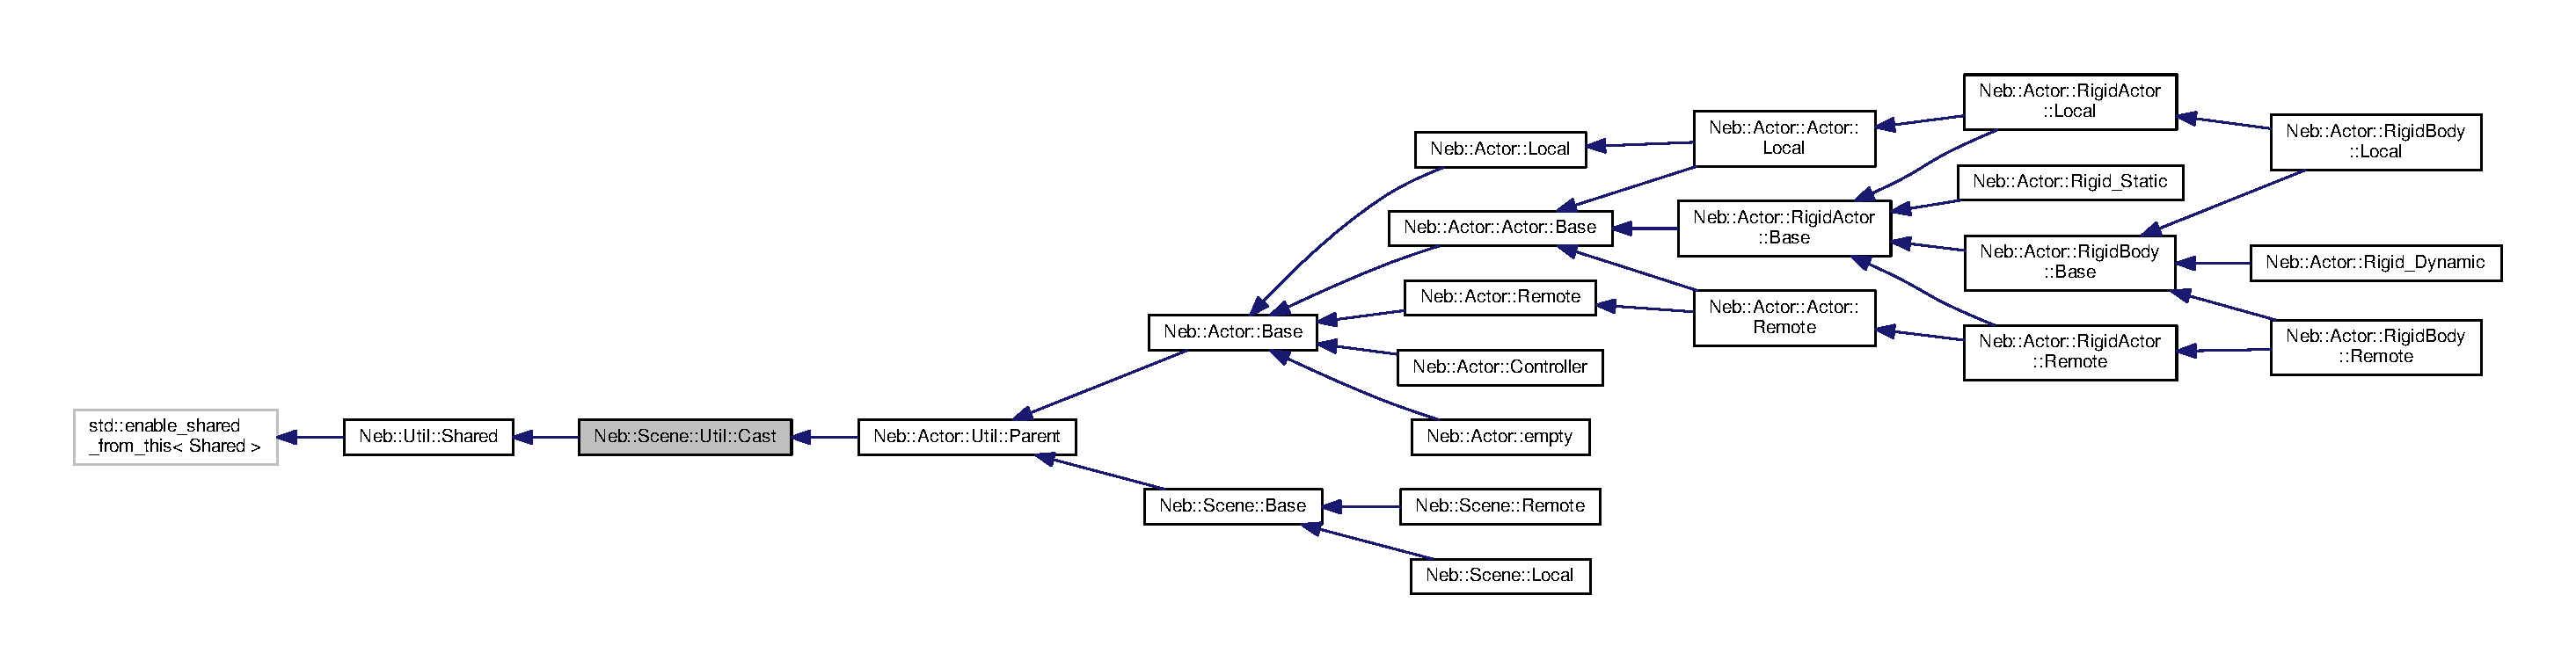
\includegraphics[width=350pt]{classNeb_1_1Scene_1_1Util_1_1Cast__inherit__graph}
\end{center}
\end{figure}


Collaboration diagram for Neb\-:\-:Scene\-:\-:Util\-:\-:Cast\-:
\nopagebreak
\begin{figure}[H]
\begin{center}
\leavevmode
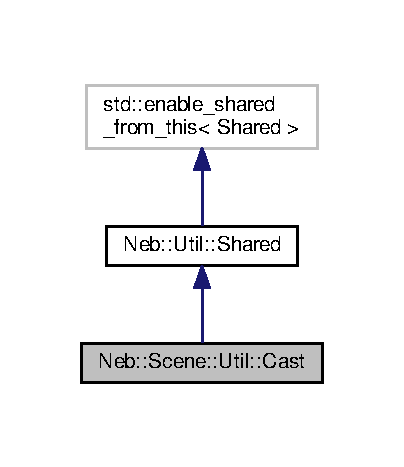
\includegraphics[width=194pt]{classNeb_1_1Scene_1_1Util_1_1Cast__coll__graph}
\end{center}
\end{figure}
\subsection*{Public Member Functions}
\begin{DoxyCompactItemize}
\item 
\hypertarget{classNeb_1_1Scene_1_1Util_1_1Cast_a53c12edc6e698f1f5f4889fc54f4f9ee}{Neb\-::\-Scene\-::\-Base\-\_\-s {\bfseries is\-Scene\-Base} ()}\label{classNeb_1_1Scene_1_1Util_1_1Cast_a53c12edc6e698f1f5f4889fc54f4f9ee}

\end{DoxyCompactItemize}


The documentation for this class was generated from the following files\-:\begin{DoxyCompactItemize}
\item 
src/\-Nebula/\-Scene/\-Util/Cast.\-hh\item 
src/\-Nebula/\-Scene/\-Util/Cast.\-cc\end{DoxyCompactItemize}

\hypertarget{classNeb_1_1Shape_1_1Util_1_1Cast}{\section{\-Neb\-:\-:\-Shape\-:\-:\-Util\-:\-:\-Cast \-Class \-Reference}
\label{classNeb_1_1Shape_1_1Util_1_1Cast}\index{\-Neb\-::\-Shape\-::\-Util\-::\-Cast@{\-Neb\-::\-Shape\-::\-Util\-::\-Cast}}
}


\-Inheritance diagram for \-Neb\-:\-:\-Shape\-:\-:\-Util\-:\-:\-Cast\-:\nopagebreak
\begin{figure}[H]
\begin{center}
\leavevmode
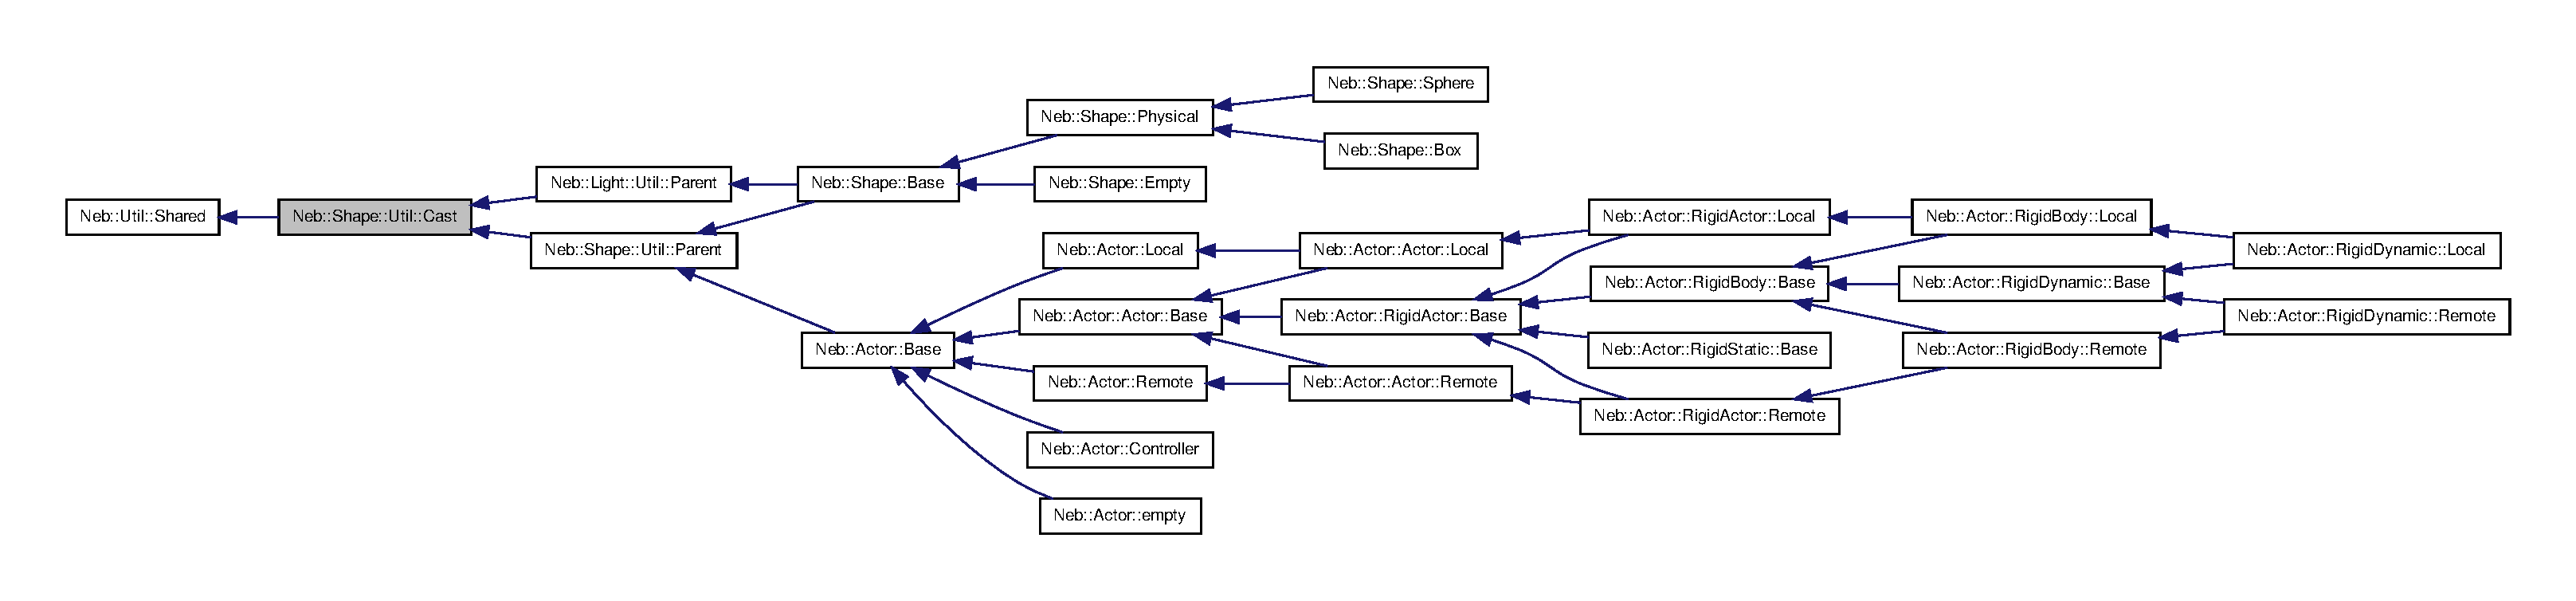
\includegraphics[width=350pt]{classNeb_1_1Shape_1_1Util_1_1Cast__inherit__graph}
\end{center}
\end{figure}


\-Collaboration diagram for \-Neb\-:\-:\-Shape\-:\-:\-Util\-:\-:\-Cast\-:\nopagebreak
\begin{figure}[H]
\begin{center}
\leavevmode
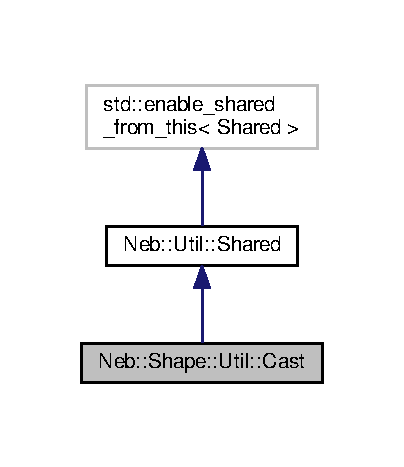
\includegraphics[width=196pt]{classNeb_1_1Shape_1_1Util_1_1Cast__coll__graph}
\end{center}
\end{figure}
\subsection*{\-Public \-Member \-Functions}
\begin{DoxyCompactItemize}
\item 
\hypertarget{classNeb_1_1Shape_1_1Util_1_1Cast_ae0f12f8f3b4bf6cf15b697249208a087}{\-Neb\-::\-Shape\-::\-Base\-\_\-s {\bfseries is\-Shape\-Base} ()}\label{classNeb_1_1Shape_1_1Util_1_1Cast_ae0f12f8f3b4bf6cf15b697249208a087}

\end{DoxyCompactItemize}


\-The documentation for this class was generated from the following file\-:\begin{DoxyCompactItemize}
\item 
src/\-Nebula/\-Shape/\-Util/\-Cast.\-hh\end{DoxyCompactItemize}

\hypertarget{classNeb_1_1Actor_1_1Util_1_1Cast}{\section{Neb\-:\-:Actor\-:\-:Util\-:\-:Cast Class Reference}
\label{classNeb_1_1Actor_1_1Util_1_1Cast}\index{Neb\-::\-Actor\-::\-Util\-::\-Cast@{Neb\-::\-Actor\-::\-Util\-::\-Cast}}
}


Inheritance diagram for Neb\-:\-:Actor\-:\-:Util\-:\-:Cast\-:
\nopagebreak
\begin{figure}[H]
\begin{center}
\leavevmode
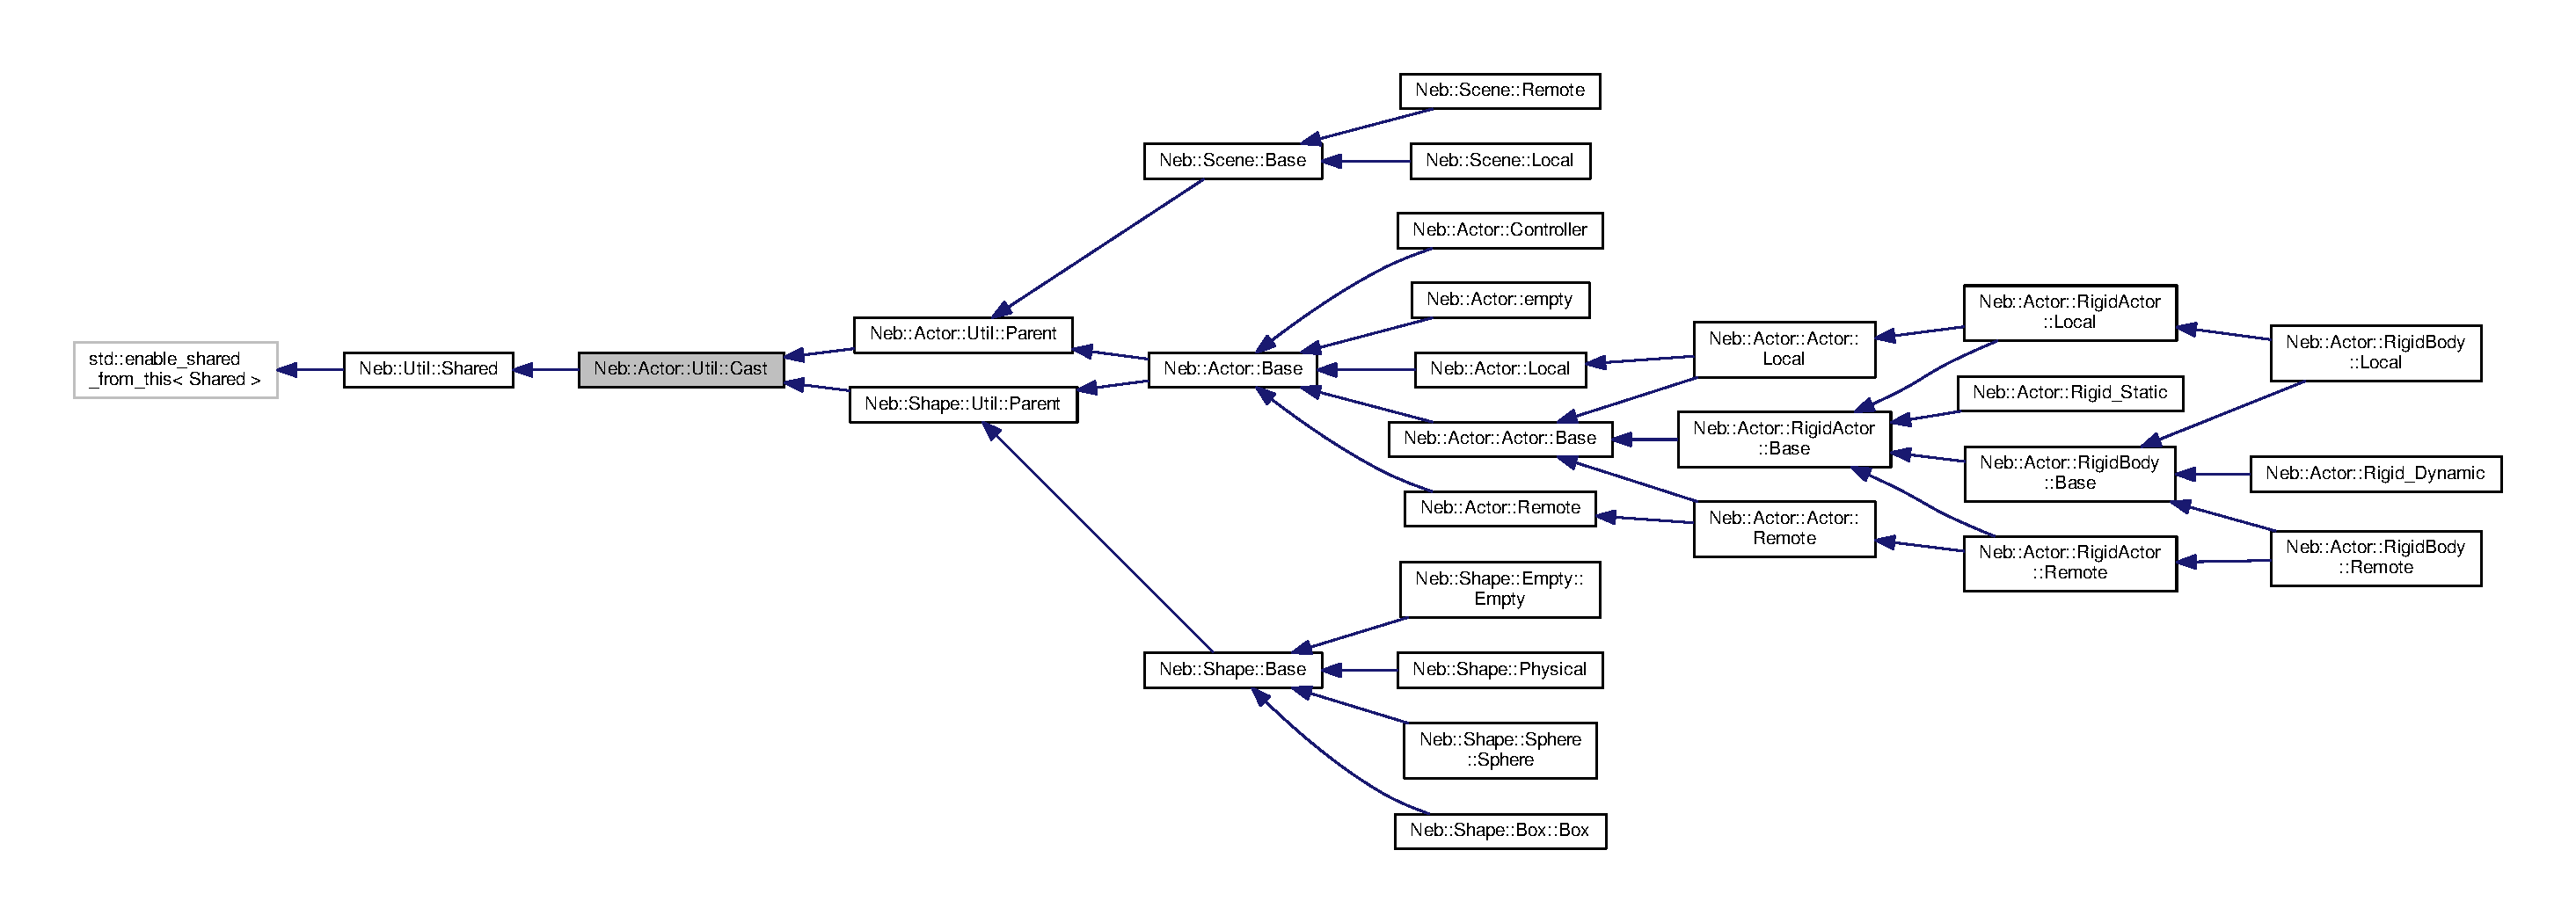
\includegraphics[width=350pt]{classNeb_1_1Actor_1_1Util_1_1Cast__inherit__graph}
\end{center}
\end{figure}


Collaboration diagram for Neb\-:\-:Actor\-:\-:Util\-:\-:Cast\-:
\nopagebreak
\begin{figure}[H]
\begin{center}
\leavevmode
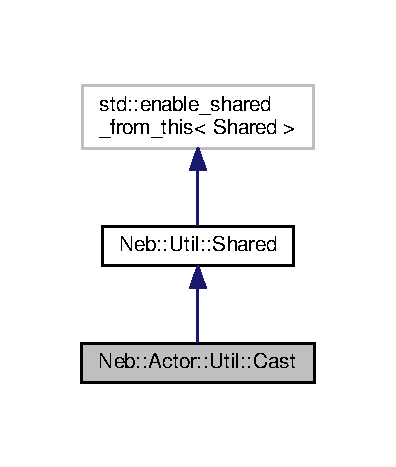
\includegraphics[width=190pt]{classNeb_1_1Actor_1_1Util_1_1Cast__coll__graph}
\end{center}
\end{figure}
\subsection*{Public Member Functions}
\begin{DoxyCompactItemize}
\item 
\hypertarget{classNeb_1_1Actor_1_1Util_1_1Cast_ab9c1dab6a3875c423ca7671cddb0cd7e}{Neb\-::\-Actor\-::\-Base\-\_\-s {\bfseries is\-Actor\-Base} ()}\label{classNeb_1_1Actor_1_1Util_1_1Cast_ab9c1dab6a3875c423ca7671cddb0cd7e}

\item 
\hypertarget{classNeb_1_1Actor_1_1Util_1_1Cast_a08ab9241db8e6bbcc7e155ac2a5df493}{Neb\-::\-Actor\-::\-Actor\-::\-Base\-\_\-s {\bfseries is\-Actor\-Actor} ()}\label{classNeb_1_1Actor_1_1Util_1_1Cast_a08ab9241db8e6bbcc7e155ac2a5df493}

\item 
\hypertarget{classNeb_1_1Actor_1_1Util_1_1Cast_a88235da713dbeded9be1efb4e53a6ca4}{Neb\-::\-Actor\-::\-Rigid\-Actor\-::\-Base\-\_\-s {\bfseries is\-Actor\-Rigid\-Actor} ()}\label{classNeb_1_1Actor_1_1Util_1_1Cast_a88235da713dbeded9be1efb4e53a6ca4}

\item 
\hypertarget{classNeb_1_1Actor_1_1Util_1_1Cast_a053d28c5b42c024dc970a5f52627c104}{Neb\-::\-Actor\-::\-Rigid\-Body\-::\-Base\-\_\-s {\bfseries is\-Actor\-Rigid\-Body} ()}\label{classNeb_1_1Actor_1_1Util_1_1Cast_a053d28c5b42c024dc970a5f52627c104}

\end{DoxyCompactItemize}


The documentation for this class was generated from the following files\-:\begin{DoxyCompactItemize}
\item 
src/\-Nebula/\-Actor/\-Util/Cast.\-hh\item 
src/\-Nebula/\-Actor/\-Util/Cast.\-cc\end{DoxyCompactItemize}

\hypertarget{classgal_1_1network_1_1client}{\section{gal\-:\-:network\-:\-:client \-Class \-Reference}
\label{classgal_1_1network_1_1client}\index{gal\-::network\-::client@{gal\-::network\-::client}}
}


socket\-\_\-client  




{\ttfamily \#include $<$client.\-hh$>$}



\-Inheritance diagram for gal\-:\-:network\-:\-:client\-:\nopagebreak
\begin{figure}[H]
\begin{center}
\leavevmode
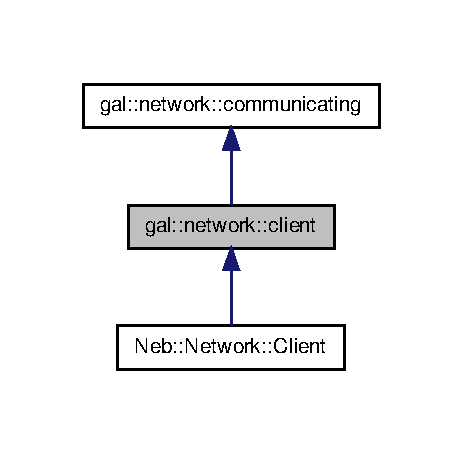
\includegraphics[width=222pt]{classgal_1_1network_1_1client__inherit__graph}
\end{center}
\end{figure}


\-Collaboration diagram for gal\-:\-:network\-:\-:client\-:\nopagebreak
\begin{figure}[H]
\begin{center}
\leavevmode
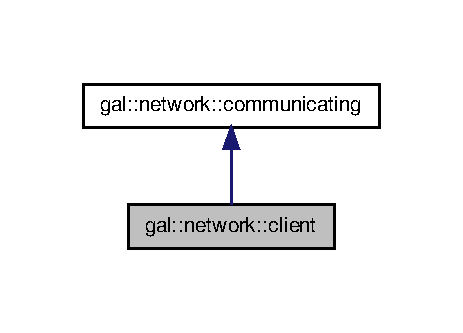
\includegraphics[width=222pt]{classgal_1_1network_1_1client__coll__graph}
\end{center}
\end{figure}
\subsection*{\-Public \-Types}
\begin{DoxyCompactItemize}
\item 
\hypertarget{classgal_1_1network_1_1client_a87ba8d69e62ce4ee5895913bf597ad6f}{typedef std\-::shared\-\_\-ptr$<$ \hyperlink{classgal_1_1network_1_1client}{client} $>$ \hyperlink{classgal_1_1network_1_1client_a87ba8d69e62ce4ee5895913bf597ad6f}{shared\-\_\-t}}\label{classgal_1_1network_1_1client_a87ba8d69e62ce4ee5895913bf597ad6f}

\begin{DoxyCompactList}\small\item\em shared\-\_\-ptr \end{DoxyCompactList}\end{DoxyCompactItemize}
\subsection*{\-Public \-Member \-Functions}
\begin{DoxyCompactItemize}
\item 
\hypertarget{classgal_1_1network_1_1client_a96e27f11ea9281a51109d3fe6e419bee}{\hyperlink{classgal_1_1network_1_1client_a96e27f11ea9281a51109d3fe6e419bee}{client} (char const $\ast$address, unsigned short port)}\label{classgal_1_1network_1_1client_a96e27f11ea9281a51109d3fe6e419bee}

\begin{DoxyCompactList}\small\item\em ctor \end{DoxyCompactList}\end{DoxyCompactItemize}
\subsection*{\-Private \-Attributes}
\begin{DoxyCompactItemize}
\item 
char const $\ast$ \hyperlink{classgal_1_1network_1_1client_a50f554a8893793fdd9e0a2d53b79f60e}{foreign\-\_\-address\-\_\-}
\begin{DoxyCompactList}\small\item\em write \end{DoxyCompactList}\item 
\hypertarget{classgal_1_1network_1_1client_acbf9159db97d571507ae2a241ee6af22}{unsigned short {\bfseries foreign\-\_\-port\-\_\-}}\label{classgal_1_1network_1_1client_acbf9159db97d571507ae2a241ee6af22}

\end{DoxyCompactItemize}


\subsection{\-Detailed \-Description}
socket\-\_\-client 

\subsection{\-Member \-Data \-Documentation}
\hypertarget{classgal_1_1network_1_1client_a50f554a8893793fdd9e0a2d53b79f60e}{\index{gal\-::network\-::client@{gal\-::network\-::client}!foreign\-\_\-address\-\_\-@{foreign\-\_\-address\-\_\-}}
\index{foreign\-\_\-address\-\_\-@{foreign\-\_\-address\-\_\-}!gal::network::client@{gal\-::network\-::client}}
\subsubsection[{foreign\-\_\-address\-\_\-}]{\setlength{\rightskip}{0pt plus 5cm}char const$\ast$ {\bf gal\-::network\-::client\-::foreign\-\_\-address\-\_\-}\hspace{0.3cm}{\ttfamily  \mbox{[}private\mbox{]}}}}\label{classgal_1_1network_1_1client_a50f554a8893793fdd9e0a2d53b79f60e}


write 

close do\-\_\-connect handle\-\_\-do\-\_\-connect 

\-The documentation for this class was generated from the following files\-:\begin{DoxyCompactItemize}
\item 
src/\-Nebula/network/client.\-hh\item 
src/\-Nebula/network/client.\-cc\item 
src/\-Nebula/network2/client.\-cc\end{DoxyCompactItemize}

\hypertarget{classNeb_1_1Network_1_1Client}{\section{\-Neb\-:\-:\-Network\-:\-:\-Client \-Class \-Reference}
\label{classNeb_1_1Network_1_1Client}\index{\-Neb\-::\-Network\-::\-Client@{\-Neb\-::\-Network\-::\-Client}}
}


\-Inheritance diagram for \-Neb\-:\-:\-Network\-:\-:\-Client\-:\nopagebreak
\begin{figure}[H]
\begin{center}
\leavevmode
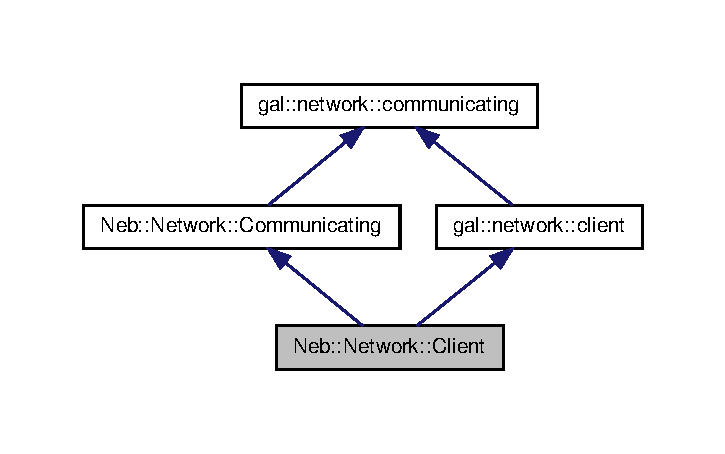
\includegraphics[width=348pt]{classNeb_1_1Network_1_1Client__inherit__graph}
\end{center}
\end{figure}


\-Collaboration diagram for \-Neb\-:\-:\-Network\-:\-:\-Client\-:\nopagebreak
\begin{figure}[H]
\begin{center}
\leavevmode
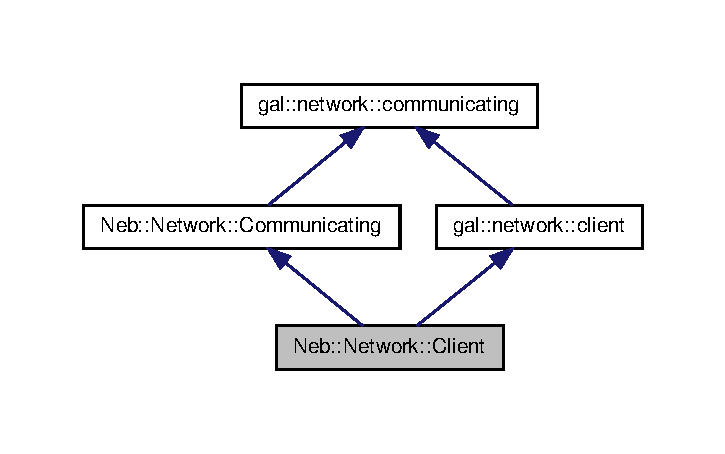
\includegraphics[width=348pt]{classNeb_1_1Network_1_1Client__coll__graph}
\end{center}
\end{figure}
\subsection*{\-Public \-Member \-Functions}
\begin{DoxyCompactItemize}
\item 
\hypertarget{classNeb_1_1Network_1_1Client_af42cd86a3ba20320503b774b4081ef20}{{\bfseries \-Client} (char const $\ast$, unsigned short)}\label{classNeb_1_1Network_1_1Client_af42cd86a3ba20320503b774b4081ef20}

\item 
\hypertarget{classNeb_1_1Network_1_1Client_a319d1d9e967e026b32b4124698a87e18}{void {\bfseries process} (gal\-::network\-::message\-\_\-s)}\label{classNeb_1_1Network_1_1Client_a319d1d9e967e026b32b4124698a87e18}

\end{DoxyCompactItemize}


\-The documentation for this class was generated from the following file\-:\begin{DoxyCompactItemize}
\item 
src/\-Nebula/network2/client.\-hh\end{DoxyCompactItemize}

\hypertarget{classNeb_1_1Color_1_1color}{\section{\-Neb\-:\-:\-Color\-:\-:color$<$ \-T $>$ \-Class \-Template \-Reference}
\label{classNeb_1_1Color_1_1color}\index{\-Neb\-::\-Color\-::color$<$ T $>$@{\-Neb\-::\-Color\-::color$<$ T $>$}}
}
\subsection*{\-Classes}
\begin{DoxyCompactItemize}
\item 
struct \hyperlink{structNeb_1_1Color_1_1color_1_1type}{type}
\end{DoxyCompactItemize}
\subsection*{\-Public \-Member \-Functions}
\begin{DoxyCompactItemize}
\item 
\hypertarget{classNeb_1_1Color_1_1color_af9fdc2ecbaef12c6adb05f77aaddc470}{{\footnotesize template$<$class Archive $>$ }\\void {\bfseries serialize} (\-Archive \&ar, unsigned int const \&version)}\label{classNeb_1_1Color_1_1color_af9fdc2ecbaef12c6adb05f77aaddc470}

\item 
\hypertarget{classNeb_1_1Color_1_1color_a0e1bf847047b917322f4ab3fca23e4af}{void {\bfseries set} (\-T new\-R, \-T new\-G, \-T new\-B, \-T new\-A)}\label{classNeb_1_1Color_1_1color_a0e1bf847047b917322f4ab3fca23e4af}

\item 
\hypertarget{classNeb_1_1Color_1_1color_a3f3767f4606d53d83bbe3757ab4c4677}{\hyperlink{classNeb_1_1Color_1_1color}{color}$<$ \-T $>$ {\bfseries rand} ()}\label{classNeb_1_1Color_1_1color_a3f3767f4606d53d83bbe3757ab4c4677}

\item 
\hypertarget{classNeb_1_1Color_1_1color_a2370eaf8a8b98a5747dcfcda64706989}{void {\bfseries set\-Black} ()}\label{classNeb_1_1Color_1_1color_a2370eaf8a8b98a5747dcfcda64706989}

\item 
\hypertarget{classNeb_1_1Color_1_1color_a68097596e5e47611a255e0c9dddce0fc}{void {\bfseries set\-White} ()}\label{classNeb_1_1Color_1_1color_a68097596e5e47611a255e0c9dddce0fc}

\item 
\hypertarget{classNeb_1_1Color_1_1color_aa8bb28a6ea4d64d8e4cee4768c2b6c83}{void {\bfseries set\-Grey} (\-T shade)}\label{classNeb_1_1Color_1_1color_aa8bb28a6ea4d64d8e4cee4768c2b6c83}

\item 
\hypertarget{classNeb_1_1Color_1_1color_a63ad81955607967426738d1ebdc8ee87}{\hyperlink{classNeb_1_1Color_1_1color}{color}$<$ \-T $>$ {\bfseries lerp} (const \hyperlink{classNeb_1_1Color_1_1color}{color} \&c2, \-T factor)}\label{classNeb_1_1Color_1_1color_a63ad81955607967426738d1ebdc8ee87}

\item 
\hypertarget{classNeb_1_1Color_1_1color_ae56aa7160b7802e9dcbbd089827ef60b}{\hyperlink{classNeb_1_1Color_1_1color}{color}$<$ \-T $>$ {\bfseries operator+} (const \hyperlink{classNeb_1_1Color_1_1color}{color} \&rhs) const }\label{classNeb_1_1Color_1_1color_ae56aa7160b7802e9dcbbd089827ef60b}

\item 
\hypertarget{classNeb_1_1Color_1_1color_a0cd903f0650e6469a832f3275c70b097}{\hyperlink{classNeb_1_1Color_1_1color}{color}$<$ \-T $>$ {\bfseries operator-\/} (const \hyperlink{classNeb_1_1Color_1_1color}{color} \&rhs) const }\label{classNeb_1_1Color_1_1color_a0cd903f0650e6469a832f3275c70b097}

\item 
\hypertarget{classNeb_1_1Color_1_1color_aca3a87ca365fd597df182463e0cbeb8e}{\hyperlink{classNeb_1_1Color_1_1color}{color}$<$ \-T $>$ {\bfseries operator$\ast$} (const \hyperlink{classNeb_1_1Color_1_1color}{color} \&rhs) const }\label{classNeb_1_1Color_1_1color_aca3a87ca365fd597df182463e0cbeb8e}

\item 
\hypertarget{classNeb_1_1Color_1_1color_aea145fdda179738004063b07c0ec2851}{\hyperlink{classNeb_1_1Color_1_1color}{color}$<$ \-T $>$ {\bfseries operator/} (const \hyperlink{classNeb_1_1Color_1_1color}{color} \&rhs) const }\label{classNeb_1_1Color_1_1color_aea145fdda179738004063b07c0ec2851}

\item 
\hypertarget{classNeb_1_1Color_1_1color_ace680db754985c4f46a5fdd1970b52b4}{\hyperlink{classNeb_1_1Color_1_1color}{color}$<$ \-T $>$ {\bfseries operator$\ast$} (const \-T rhs) const }\label{classNeb_1_1Color_1_1color_ace680db754985c4f46a5fdd1970b52b4}

\item 
\hypertarget{classNeb_1_1Color_1_1color_a25960824de5b39809c51e7ab00c5f137}{\hyperlink{classNeb_1_1Color_1_1color}{color}$<$ \-T $>$ {\bfseries operator/} (const \-T rhs) const }\label{classNeb_1_1Color_1_1color_a25960824de5b39809c51e7ab00c5f137}

\item 
\hypertarget{classNeb_1_1Color_1_1color_a2cb92150e4daf12f22791d2c058b2d3e}{bool {\bfseries operator==} (\hyperlink{classNeb_1_1Color_1_1color}{color}$<$ \-T $>$ const \&rhs) const }\label{classNeb_1_1Color_1_1color_a2cb92150e4daf12f22791d2c058b2d3e}

\item 
\hypertarget{classNeb_1_1Color_1_1color_ad4c72e79ba0510b3b46decc5c97a52b6}{bool {\bfseries operator!=} (\hyperlink{classNeb_1_1Color_1_1color}{color}$<$ \-T $>$ const \&rhs) const }\label{classNeb_1_1Color_1_1color_ad4c72e79ba0510b3b46decc5c97a52b6}

\item 
\hypertarget{classNeb_1_1Color_1_1color_a8ac20d4a0be8e91227ff3e4aa3fbf965}{\hyperlink{classNeb_1_1Color_1_1color}{color}$<$ \-T $>$ {\bfseries operator+=} (\hyperlink{classNeb_1_1Color_1_1color}{color}$<$ \-T $>$ const \&rhs)}\label{classNeb_1_1Color_1_1color_a8ac20d4a0be8e91227ff3e4aa3fbf965}

\item 
\hypertarget{classNeb_1_1Color_1_1color_a11d806e2180d966e321d793279a74768}{\hyperlink{classNeb_1_1Color_1_1color}{color}$<$ \-T $>$ {\bfseries operator-\/=} (\hyperlink{classNeb_1_1Color_1_1color}{color}$<$ \-T $>$ const \&rhs)}\label{classNeb_1_1Color_1_1color_a11d806e2180d966e321d793279a74768}

\item 
\hypertarget{classNeb_1_1Color_1_1color_a9415df05e06e0f9c8df77a31d57a0445}{\hyperlink{classNeb_1_1Color_1_1color}{color}$<$ \-T $>$ {\bfseries operator$\ast$=} (const \hyperlink{classNeb_1_1Color_1_1color}{color} \&rhs)}\label{classNeb_1_1Color_1_1color_a9415df05e06e0f9c8df77a31d57a0445}

\item 
\hypertarget{classNeb_1_1Color_1_1color_ac433ff6e88f5321553cde4fbbcc44c93}{\hyperlink{classNeb_1_1Color_1_1color}{color}$<$ \-T $>$ {\bfseries operator/=} (const \hyperlink{classNeb_1_1Color_1_1color}{color} \&rhs)}\label{classNeb_1_1Color_1_1color_ac433ff6e88f5321553cde4fbbcc44c93}

\item 
\hypertarget{classNeb_1_1Color_1_1color_abf6ec35bb77ff7e41d4fc1df71cee68c}{\hyperlink{classNeb_1_1Color_1_1color}{color}$<$ \-T $>$ {\bfseries operator$\ast$=} (const \-T rhs)}\label{classNeb_1_1Color_1_1color_abf6ec35bb77ff7e41d4fc1df71cee68c}

\item 
\hypertarget{classNeb_1_1Color_1_1color_ada4906a4072c6e8d9f612049821dda09}{\hyperlink{classNeb_1_1Color_1_1color}{color}$<$ \-T $>$ {\bfseries operator/=} (const \-T rhs)}\label{classNeb_1_1Color_1_1color_ada4906a4072c6e8d9f612049821dda09}

\item 
\hypertarget{classNeb_1_1Color_1_1color_afa0997e04f77dd7e67fa3f6fab5a29a2}{\hyperlink{classNeb_1_1Color_1_1color}{color}$<$ \-T $>$ {\bfseries operator-\/} () const }\label{classNeb_1_1Color_1_1color_afa0997e04f77dd7e67fa3f6fab5a29a2}

\item 
\hypertarget{classNeb_1_1Color_1_1color_ab7bebf143bd8a33803d834ca8f905f60}{\hyperlink{classNeb_1_1Color_1_1color}{color}$<$ \-T $>$ {\bfseries operator+} () const }\label{classNeb_1_1Color_1_1color_ab7bebf143bd8a33803d834ca8f905f60}

\item 
\hypertarget{classNeb_1_1Color_1_1color_a719d9a58af338b802ea111dd497248c5}{void {\bfseries clamp\-To01} ()}\label{classNeb_1_1Color_1_1color_a719d9a58af338b802ea111dd497248c5}

\item 
\hypertarget{classNeb_1_1Color_1_1color_a1716749ce6a7c48de144a3df85e31167}{void {\bfseries print} ()}\label{classNeb_1_1Color_1_1color_a1716749ce6a7c48de144a3df85e31167}

\item 
\hypertarget{classNeb_1_1Color_1_1color_a5f6798b63d8c5041429b9337b574a6bd}{\-T {\bfseries saw} (\-T t, \-T f)}\label{classNeb_1_1Color_1_1color_a5f6798b63d8c5041429b9337b574a6bd}

\item 
\hypertarget{classNeb_1_1Color_1_1color_af1d98f24d2f9099adeb0240321eb1b7c}{\hyperlink{classNeb_1_1Color_1_1color}{color}$<$ \-T $>$ {\bfseries operator$\ast$} (\-T f)}\label{classNeb_1_1Color_1_1color_af1d98f24d2f9099adeb0240321eb1b7c}

\item 
\hypertarget{classNeb_1_1Color_1_1color_a38dbc69cf80201fcc85a617be2aa9ee8}{{\bfseries operator T $\ast$} () const }\label{classNeb_1_1Color_1_1color_a38dbc69cf80201fcc85a617be2aa9ee8}

\item 
\hypertarget{classNeb_1_1Color_1_1color_ad92e1e077bc6cd7d26993bfdedbdbb1a}{{\bfseries operator T const $\ast$} () const }\label{classNeb_1_1Color_1_1color_ad92e1e077bc6cd7d26993bfdedbdbb1a}

\end{DoxyCompactItemize}
\begin{Indent}{\bf \-Constructor}\par
\begin{DoxyCompactItemize}
\item 
\hypertarget{classNeb_1_1Color_1_1color_ab35009014a60a8126f597652117ffb5f}{{\bfseries color} ()}\label{classNeb_1_1Color_1_1color_ab35009014a60a8126f597652117ffb5f}

\item 
\hypertarget{classNeb_1_1Color_1_1color_a4e42ac5e9bc44c84ce795e0a017f1081}{{\bfseries color} (\-T new\-R, \-T new\-G, \-T new\-B, \-T new\-A)}\label{classNeb_1_1Color_1_1color_a4e42ac5e9bc44c84ce795e0a017f1081}

\item 
\hypertarget{classNeb_1_1Color_1_1color_aae5bfdbef12648b87d39d5348af2d7ed}{{\bfseries color} (const \hyperlink{classNeb_1_1Color_1_1color}{color} \&rhs)}\label{classNeb_1_1Color_1_1color_aae5bfdbef12648b87d39d5348af2d7ed}

\end{DoxyCompactItemize}
\end{Indent}
\subsection*{\-Public \-Attributes}
\begin{DoxyCompactItemize}
\item 
\hypertarget{classNeb_1_1Color_1_1color_a8a18346bc363bf76e839492605e0a1f4}{\-T {\bfseries r}}\label{classNeb_1_1Color_1_1color_a8a18346bc363bf76e839492605e0a1f4}

\item 
\hypertarget{classNeb_1_1Color_1_1color_a681638c1b8b3e75508c654c3b356d07c}{\-T {\bfseries g}}\label{classNeb_1_1Color_1_1color_a681638c1b8b3e75508c654c3b356d07c}

\item 
\hypertarget{classNeb_1_1Color_1_1color_a7db460b59724724bbe4d1696a72bb3dc}{\-T {\bfseries b}}\label{classNeb_1_1Color_1_1color_a7db460b59724724bbe4d1696a72bb3dc}

\item 
\hypertarget{classNeb_1_1Color_1_1color_ad30391f20a88d4ea5be687113821be7e}{\-T {\bfseries a}}\label{classNeb_1_1Color_1_1color_ad30391f20a88d4ea5be687113821be7e}

\end{DoxyCompactItemize}
\subsubsection*{template$<$typename \-T$>$ class Neb\-::\-Color\-::color$<$ T $>$}



\-The documentation for this class was generated from the following file\-:\begin{DoxyCompactItemize}
\item 
src/\-Nebula/\-Graphics/\-Color/\-Color.\-hh\end{DoxyCompactItemize}

\hypertarget{classgal_1_1network_1_1communicating}{\section{gal\-:\-:network\-:\-:communicating \-Class \-Reference}
\label{classgal_1_1network_1_1communicating}\index{gal\-::network\-::communicating@{gal\-::network\-::communicating}}
}


{\ttfamily \#include $<$communicating.\-hpp$>$}



\-Inheritance diagram for gal\-:\-:network\-:\-:communicating\-:\nopagebreak
\begin{figure}[H]
\begin{center}
\leavevmode
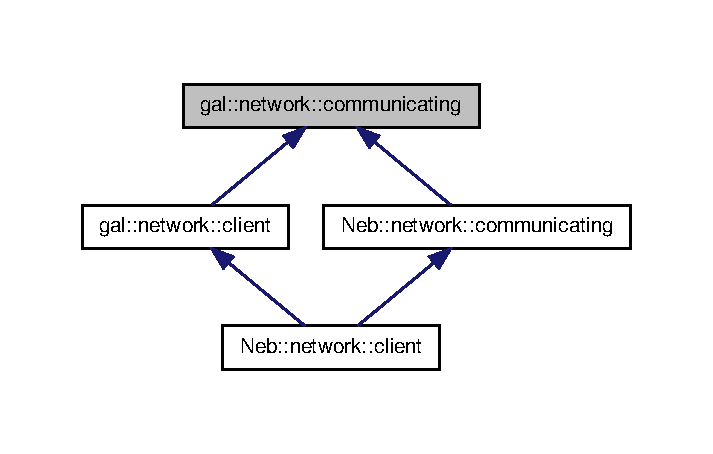
\includegraphics[width=222pt]{classgal_1_1network_1_1communicating__inherit__graph}
\end{center}
\end{figure}
\subsection*{\-Public \-Types}
\begin{DoxyCompactItemize}
\item 
enum \{ {\bfseries \-M\-A\-X\-\_\-\-M\-E\-S\-S\-A\-G\-E\-\_\-\-L\-E\-N\-G\-T\-H} =  10000
 \}
\item 
\hypertarget{classgal_1_1network_1_1communicating_aef6c11aca9b227ec65e289b5f194cd83}{typedef int {\bfseries \-H\-E\-A\-D\-E\-R\-\_\-\-T\-Y\-P\-E}}\label{classgal_1_1network_1_1communicating_aef6c11aca9b227ec65e289b5f194cd83}

\item 
\hypertarget{classgal_1_1network_1_1communicating_a20c6f2dc53a296b6b34a82d5dc8f894a}{typedef std\-::shared\-\_\-ptr\*
$<$ \hyperlink{classgal_1_1network_1_1communicating}{communicating} $>$ {\bfseries shared\-\_\-t}}\label{classgal_1_1network_1_1communicating_a20c6f2dc53a296b6b34a82d5dc8f894a}

\item 
\hypertarget{classgal_1_1network_1_1communicating_acde720b70acbd7aecc86d2ebd4d91113}{typedef std\-::vector$<$ shared\-\_\-t $>$ {\bfseries vector\-\_\-t}}\label{classgal_1_1network_1_1communicating_acde720b70acbd7aecc86d2ebd4d91113}

\end{DoxyCompactItemize}
\subsection*{\-Public \-Member \-Functions}
\begin{DoxyCompactItemize}
\item 
\hyperlink{classgal_1_1network_1_1communicating_a151e8a718480e38a21ee0a953dc4b57f}{communicating} (int socket)
\item 
void \hyperlink{classgal_1_1network_1_1communicating_a388de6dcc741701cffaea874898643e6}{write} (boost\-::shared\-\_\-ptr$<$ \hyperlink{classgal_1_1network_1_1message}{message} $>$)
\item 
void \hyperlink{classgal_1_1network_1_1communicating_a3b39dcb940d746f44b6c2c72e198450d}{close} ()
\item 
void \hyperlink{classgal_1_1network_1_1communicating_a43bf55d2d11f1798b4814e069639a239}{start} ()
\item 
\hypertarget{classgal_1_1network_1_1communicating_aa9eb8cf91d093cbf9cd7293e8f10122e}{virtual void {\bfseries process} (boost\-::shared\-\_\-ptr$<$ \hyperlink{classgal_1_1network_1_1message}{message} $>$)=0}\label{classgal_1_1network_1_1communicating_aa9eb8cf91d093cbf9cd7293e8f10122e}

\item 
void \hyperlink{classgal_1_1network_1_1communicating_a271caa9e5d4d13fffda9d38218231b2c}{thread\-\_\-write} (boost\-::shared\-\_\-ptr$<$ \hyperlink{classgal_1_1network_1_1message}{message} $>$)
\item 
void \hyperlink{classgal_1_1network_1_1communicating_a32da51cf806bdc60b1a653ef20557af9}{thread\-\_\-write\-\_\-dispatch} ()
\item 
void \hyperlink{classgal_1_1network_1_1communicating_abd5efaa6563dda2097f69ae3679f87a1}{thread\-\_\-read} ()
\item 
void \hyperlink{classgal_1_1network_1_1communicating_aa7ef767d5117ba5d99cddcb1d7696a1d}{thread\-\_\-read\-\_\-header} ()
\item 
void \hyperlink{classgal_1_1network_1_1communicating_aeba5f8e491d9c6a4ddd75aa0a698bed9}{thread\-\_\-read\-\_\-body} ()
\item 
void \hyperlink{classgal_1_1network_1_1communicating_ab1434959e6a6b7311e7189078679124f}{handle\-\_\-do\-\_\-read\-\_\-header} ()
\item 
void \hyperlink{classgal_1_1network_1_1communicating_a383465f75d9d656a0e80ea3f57963630}{handle\-\_\-do\-\_\-read\-\_\-body} ()
\item 
void \hyperlink{classgal_1_1network_1_1communicating_a5a0d9fbfe61ff1d35380854d8aa3860e}{handle\-\_\-do\-\_\-write} ()
\end{DoxyCompactItemize}
\subsection*{\-Protected \-Attributes}
\begin{DoxyCompactItemize}
\item 
int \hyperlink{classgal_1_1network_1_1communicating_afe5f9de9e2535e261c78485dec4d9e82}{socket\-\_\-}
\end{DoxyCompactItemize}
\subsection*{\-Private \-Attributes}
\begin{DoxyCompactItemize}
\item 
\hypertarget{classgal_1_1network_1_1communicating_addb0099bce03feeb9ff20a5244976c54}{\-H\-E\-A\-D\-E\-R\-\_\-\-T\-Y\-P\-E {\bfseries write\-\_\-header\-\_\-}}\label{classgal_1_1network_1_1communicating_addb0099bce03feeb9ff20a5244976c54}

\item 
std\-::deque$<$ boost\-::shared\-\_\-ptr\*
$<$ \hyperlink{classgal_1_1network_1_1message}{message} $>$ $>$ \hyperlink{classgal_1_1network_1_1communicating_a5d0757e59bab953f76f65edfc1b3bd15}{write\-\_\-queue\-\_\-}
\item 
bool \hyperlink{classgal_1_1network_1_1communicating_a4dc031687aa84ce7e3cca5ce9839d5d7}{terminate\-\_\-}
\item 
std\-::thread \hyperlink{classgal_1_1network_1_1communicating_afc83d88ea30befb842e16a5cf7d5e936}{write\-\_\-thread\-\_\-}
\item 
std\-::thread \hyperlink{classgal_1_1network_1_1communicating_a2d94e9fcd2cd765768b354a87b726bf3}{read\-\_\-thread\-\_\-}
\item 
std\-::condition\-\_\-variable \hyperlink{classgal_1_1network_1_1communicating_aff2d38da260c4e5f9182eec6f8bc16bd}{cv\-\_\-}
\item 
\hypertarget{classgal_1_1network_1_1communicating_ac1027b607900f3d087baac99aba3507e}{std\-::condition\-\_\-variable {\bfseries cv\-\_\-ready\-\_\-}}\label{classgal_1_1network_1_1communicating_ac1027b607900f3d087baac99aba3507e}

\item 
std\-::mutex \hyperlink{classgal_1_1network_1_1communicating_a7afe6898e58ca9087f05124cf4d18b65}{mutex\-\_\-}
\item 
\hypertarget{classgal_1_1network_1_1communicating_a6f59c7c2c3034687f96369a9c76cc90b}{std\-::mutex {\bfseries mutex\-\_\-start\-\_\-}}\label{classgal_1_1network_1_1communicating_a6f59c7c2c3034687f96369a9c76cc90b}

\end{DoxyCompactItemize}
\begin{Indent}{\bf \-Read \-Data \-Members @\{}\par
\begin{DoxyCompactItemize}
\item 
\hypertarget{classgal_1_1network_1_1communicating_ad9d721c71a996f044175a10741341bf8}{boost\-::shared\-\_\-ptr$<$ \hyperlink{classgal_1_1network_1_1message}{message} $>$ {\bfseries read\-\_\-msg\-\_\-}}\label{classgal_1_1network_1_1communicating_ad9d721c71a996f044175a10741341bf8}

\item 
\hypertarget{classgal_1_1network_1_1communicating_aab4813fff665c6d4379ba8f410f97bd7}{\-H\-E\-A\-D\-E\-R\-\_\-\-T\-Y\-P\-E {\bfseries read\-\_\-header\-\_\-}}\label{classgal_1_1network_1_1communicating_aab4813fff665c6d4379ba8f410f97bd7}

\item 
\hypertarget{classgal_1_1network_1_1communicating_aa33fdc45c281e7664950a272e63b585f}{char {\bfseries read\-\_\-buffer\-\_\-} \mbox{[}\-M\-A\-X\-\_\-\-M\-E\-S\-S\-A\-G\-E\-\_\-\-L\-E\-N\-G\-T\-H\mbox{]}}\label{classgal_1_1network_1_1communicating_aa33fdc45c281e7664950a272e63b585f}

\end{DoxyCompactItemize}
\end{Indent}


\subsection{\-Detailed \-Description}
socket communicating 

\subsection{\-Constructor \& \-Destructor \-Documentation}
\hypertarget{classgal_1_1network_1_1communicating_a151e8a718480e38a21ee0a953dc4b57f}{\index{gal\-::network\-::communicating@{gal\-::network\-::communicating}!communicating@{communicating}}
\index{communicating@{communicating}!gal::network::communicating@{gal\-::network\-::communicating}}
\subsubsection[{communicating}]{\setlength{\rightskip}{0pt plus 5cm}{\bf gal\-::network\-::communicating\-::communicating} (
\begin{DoxyParamCaption}
\item[{int}]{socket}
\end{DoxyParamCaption}
)}}\label{classgal_1_1network_1_1communicating_a151e8a718480e38a21ee0a953dc4b57f}
ctor 

\subsection{\-Member \-Function \-Documentation}
\hypertarget{classgal_1_1network_1_1communicating_a3b39dcb940d746f44b6c2c72e198450d}{\index{gal\-::network\-::communicating@{gal\-::network\-::communicating}!close@{close}}
\index{close@{close}!gal::network::communicating@{gal\-::network\-::communicating}}
\subsubsection[{close}]{\setlength{\rightskip}{0pt plus 5cm}void {\bf gal\-::network\-::communicating\-::close} (
\begin{DoxyParamCaption}
{}
\end{DoxyParamCaption}
)}}\label{classgal_1_1network_1_1communicating_a3b39dcb940d746f44b6c2c72e198450d}
close \hypertarget{classgal_1_1network_1_1communicating_a383465f75d9d656a0e80ea3f57963630}{\index{gal\-::network\-::communicating@{gal\-::network\-::communicating}!handle\-\_\-do\-\_\-read\-\_\-body@{handle\-\_\-do\-\_\-read\-\_\-body}}
\index{handle\-\_\-do\-\_\-read\-\_\-body@{handle\-\_\-do\-\_\-read\-\_\-body}!gal::network::communicating@{gal\-::network\-::communicating}}
\subsubsection[{handle\-\_\-do\-\_\-read\-\_\-body}]{\setlength{\rightskip}{0pt plus 5cm}void {\bf gal\-::network\-::communicating\-::handle\-\_\-do\-\_\-read\-\_\-body} (
\begin{DoxyParamCaption}
{}
\end{DoxyParamCaption}
)}}\label{classgal_1_1network_1_1communicating_a383465f75d9d656a0e80ea3f57963630}
handle read body \hypertarget{classgal_1_1network_1_1communicating_ab1434959e6a6b7311e7189078679124f}{\index{gal\-::network\-::communicating@{gal\-::network\-::communicating}!handle\-\_\-do\-\_\-read\-\_\-header@{handle\-\_\-do\-\_\-read\-\_\-header}}
\index{handle\-\_\-do\-\_\-read\-\_\-header@{handle\-\_\-do\-\_\-read\-\_\-header}!gal::network::communicating@{gal\-::network\-::communicating}}
\subsubsection[{handle\-\_\-do\-\_\-read\-\_\-header}]{\setlength{\rightskip}{0pt plus 5cm}void {\bf gal\-::network\-::communicating\-::handle\-\_\-do\-\_\-read\-\_\-header} (
\begin{DoxyParamCaption}
{}
\end{DoxyParamCaption}
)}}\label{classgal_1_1network_1_1communicating_ab1434959e6a6b7311e7189078679124f}
handle read header \hypertarget{classgal_1_1network_1_1communicating_a5a0d9fbfe61ff1d35380854d8aa3860e}{\index{gal\-::network\-::communicating@{gal\-::network\-::communicating}!handle\-\_\-do\-\_\-write@{handle\-\_\-do\-\_\-write}}
\index{handle\-\_\-do\-\_\-write@{handle\-\_\-do\-\_\-write}!gal::network::communicating@{gal\-::network\-::communicating}}
\subsubsection[{handle\-\_\-do\-\_\-write}]{\setlength{\rightskip}{0pt plus 5cm}void {\bf gal\-::network\-::communicating\-::handle\-\_\-do\-\_\-write} (
\begin{DoxyParamCaption}
{}
\end{DoxyParamCaption}
)}}\label{classgal_1_1network_1_1communicating_a5a0d9fbfe61ff1d35380854d8aa3860e}
handle write \hypertarget{classgal_1_1network_1_1communicating_a43bf55d2d11f1798b4814e069639a239}{\index{gal\-::network\-::communicating@{gal\-::network\-::communicating}!start@{start}}
\index{start@{start}!gal::network::communicating@{gal\-::network\-::communicating}}
\subsubsection[{start}]{\setlength{\rightskip}{0pt plus 5cm}void {\bf gal\-::network\-::communicating\-::start} (
\begin{DoxyParamCaption}
{}
\end{DoxyParamCaption}
)}}\label{classgal_1_1network_1_1communicating_a43bf55d2d11f1798b4814e069639a239}
thread write \hypertarget{classgal_1_1network_1_1communicating_abd5efaa6563dda2097f69ae3679f87a1}{\index{gal\-::network\-::communicating@{gal\-::network\-::communicating}!thread\-\_\-read@{thread\-\_\-read}}
\index{thread\-\_\-read@{thread\-\_\-read}!gal::network::communicating@{gal\-::network\-::communicating}}
\subsubsection[{thread\-\_\-read}]{\setlength{\rightskip}{0pt plus 5cm}void {\bf gal\-::network\-::communicating\-::thread\-\_\-read} (
\begin{DoxyParamCaption}
{}
\end{DoxyParamCaption}
)}}\label{classgal_1_1network_1_1communicating_abd5efaa6563dda2097f69ae3679f87a1}
thread read \begin{DoxyRefDesc}{\-Todo}
\item[\hyperlink{todo__todo000008}{\-Todo}]pass exception to main thread ( or whoever ) \end{DoxyRefDesc}
\hypertarget{classgal_1_1network_1_1communicating_aeba5f8e491d9c6a4ddd75aa0a698bed9}{\index{gal\-::network\-::communicating@{gal\-::network\-::communicating}!thread\-\_\-read\-\_\-body@{thread\-\_\-read\-\_\-body}}
\index{thread\-\_\-read\-\_\-body@{thread\-\_\-read\-\_\-body}!gal::network::communicating@{gal\-::network\-::communicating}}
\subsubsection[{thread\-\_\-read\-\_\-body}]{\setlength{\rightskip}{0pt plus 5cm}void {\bf gal\-::network\-::communicating\-::thread\-\_\-read\-\_\-body} (
\begin{DoxyParamCaption}
{}
\end{DoxyParamCaption}
)}}\label{classgal_1_1network_1_1communicating_aeba5f8e491d9c6a4ddd75aa0a698bed9}
thread read body \hypertarget{classgal_1_1network_1_1communicating_aa7ef767d5117ba5d99cddcb1d7696a1d}{\index{gal\-::network\-::communicating@{gal\-::network\-::communicating}!thread\-\_\-read\-\_\-header@{thread\-\_\-read\-\_\-header}}
\index{thread\-\_\-read\-\_\-header@{thread\-\_\-read\-\_\-header}!gal::network::communicating@{gal\-::network\-::communicating}}
\subsubsection[{thread\-\_\-read\-\_\-header}]{\setlength{\rightskip}{0pt plus 5cm}void {\bf gal\-::network\-::communicating\-::thread\-\_\-read\-\_\-header} (
\begin{DoxyParamCaption}
{}
\end{DoxyParamCaption}
)}}\label{classgal_1_1network_1_1communicating_aa7ef767d5117ba5d99cddcb1d7696a1d}
thread read header \hypertarget{classgal_1_1network_1_1communicating_a271caa9e5d4d13fffda9d38218231b2c}{\index{gal\-::network\-::communicating@{gal\-::network\-::communicating}!thread\-\_\-write@{thread\-\_\-write}}
\index{thread\-\_\-write@{thread\-\_\-write}!gal::network::communicating@{gal\-::network\-::communicating}}
\subsubsection[{thread\-\_\-write}]{\setlength{\rightskip}{0pt plus 5cm}void {\bf gal\-::network\-::communicating\-::thread\-\_\-write} (
\begin{DoxyParamCaption}
\item[{boost\-::shared\-\_\-ptr$<$ {\bf message} $>$}]{}
\end{DoxyParamCaption}
)}}\label{classgal_1_1network_1_1communicating_a271caa9e5d4d13fffda9d38218231b2c}
\begin{DoxyRefDesc}{\-Todo}
\item[\hyperlink{todo__todo000007}{\-Todo}]pass exception to main thread ( or whoever ) \end{DoxyRefDesc}
\hypertarget{classgal_1_1network_1_1communicating_a32da51cf806bdc60b1a653ef20557af9}{\index{gal\-::network\-::communicating@{gal\-::network\-::communicating}!thread\-\_\-write\-\_\-dispatch@{thread\-\_\-write\-\_\-dispatch}}
\index{thread\-\_\-write\-\_\-dispatch@{thread\-\_\-write\-\_\-dispatch}!gal::network::communicating@{gal\-::network\-::communicating}}
\subsubsection[{thread\-\_\-write\-\_\-dispatch}]{\setlength{\rightskip}{0pt plus 5cm}void {\bf gal\-::network\-::communicating\-::thread\-\_\-write\-\_\-dispatch} (
\begin{DoxyParamCaption}
{}
\end{DoxyParamCaption}
)}}\label{classgal_1_1network_1_1communicating_a32da51cf806bdc60b1a653ef20557af9}
thread write dispath \hypertarget{classgal_1_1network_1_1communicating_a388de6dcc741701cffaea874898643e6}{\index{gal\-::network\-::communicating@{gal\-::network\-::communicating}!write@{write}}
\index{write@{write}!gal::network::communicating@{gal\-::network\-::communicating}}
\subsubsection[{write}]{\setlength{\rightskip}{0pt plus 5cm}void {\bf gal\-::network\-::communicating\-::write} (
\begin{DoxyParamCaption}
\item[{boost\-::shared\-\_\-ptr$<$ {\bf message} $>$}]{}
\end{DoxyParamCaption}
)}}\label{classgal_1_1network_1_1communicating_a388de6dcc741701cffaea874898643e6}
write 

\subsection{\-Member \-Data \-Documentation}
\hypertarget{classgal_1_1network_1_1communicating_aff2d38da260c4e5f9182eec6f8bc16bd}{\index{gal\-::network\-::communicating@{gal\-::network\-::communicating}!cv\-\_\-@{cv\-\_\-}}
\index{cv\-\_\-@{cv\-\_\-}!gal::network::communicating@{gal\-::network\-::communicating}}
\subsubsection[{cv\-\_\-}]{\setlength{\rightskip}{0pt plus 5cm}std\-::condition\-\_\-variable {\bf gal\-::network\-::communicating\-::cv\-\_\-}\hspace{0.3cm}{\ttfamily  \mbox{[}private\mbox{]}}}}\label{classgal_1_1network_1_1communicating_aff2d38da260c4e5f9182eec6f8bc16bd}
condition variable \hypertarget{classgal_1_1network_1_1communicating_a7afe6898e58ca9087f05124cf4d18b65}{\index{gal\-::network\-::communicating@{gal\-::network\-::communicating}!mutex\-\_\-@{mutex\-\_\-}}
\index{mutex\-\_\-@{mutex\-\_\-}!gal::network::communicating@{gal\-::network\-::communicating}}
\subsubsection[{mutex\-\_\-}]{\setlength{\rightskip}{0pt plus 5cm}std\-::mutex {\bf gal\-::network\-::communicating\-::mutex\-\_\-}\hspace{0.3cm}{\ttfamily  \mbox{[}private\mbox{]}}}}\label{classgal_1_1network_1_1communicating_a7afe6898e58ca9087f05124cf4d18b65}
mutex mutex for write\-\_\-queue\-\_\- and terminate\-\_\- \hypertarget{classgal_1_1network_1_1communicating_a2d94e9fcd2cd765768b354a87b726bf3}{\index{gal\-::network\-::communicating@{gal\-::network\-::communicating}!read\-\_\-thread\-\_\-@{read\-\_\-thread\-\_\-}}
\index{read\-\_\-thread\-\_\-@{read\-\_\-thread\-\_\-}!gal::network::communicating@{gal\-::network\-::communicating}}
\subsubsection[{read\-\_\-thread\-\_\-}]{\setlength{\rightskip}{0pt plus 5cm}std\-::thread {\bf gal\-::network\-::communicating\-::read\-\_\-thread\-\_\-}\hspace{0.3cm}{\ttfamily  \mbox{[}private\mbox{]}}}}\label{classgal_1_1network_1_1communicating_a2d94e9fcd2cd765768b354a87b726bf3}
thread read \hypertarget{classgal_1_1network_1_1communicating_afe5f9de9e2535e261c78485dec4d9e82}{\index{gal\-::network\-::communicating@{gal\-::network\-::communicating}!socket\-\_\-@{socket\-\_\-}}
\index{socket\-\_\-@{socket\-\_\-}!gal::network::communicating@{gal\-::network\-::communicating}}
\subsubsection[{socket\-\_\-}]{\setlength{\rightskip}{0pt plus 5cm}int {\bf gal\-::network\-::communicating\-::socket\-\_\-}\hspace{0.3cm}{\ttfamily  \mbox{[}protected\mbox{]}}}}\label{classgal_1_1network_1_1communicating_afe5f9de9e2535e261c78485dec4d9e82}
socket \hypertarget{classgal_1_1network_1_1communicating_a4dc031687aa84ce7e3cca5ce9839d5d7}{\index{gal\-::network\-::communicating@{gal\-::network\-::communicating}!terminate\-\_\-@{terminate\-\_\-}}
\index{terminate\-\_\-@{terminate\-\_\-}!gal::network::communicating@{gal\-::network\-::communicating}}
\subsubsection[{terminate\-\_\-}]{\setlength{\rightskip}{0pt plus 5cm}bool {\bf gal\-::network\-::communicating\-::terminate\-\_\-}\hspace{0.3cm}{\ttfamily  \mbox{[}private\mbox{]}}}}\label{classgal_1_1network_1_1communicating_a4dc031687aa84ce7e3cca5ce9839d5d7}
process body \hypertarget{classgal_1_1network_1_1communicating_a5d0757e59bab953f76f65edfc1b3bd15}{\index{gal\-::network\-::communicating@{gal\-::network\-::communicating}!write\-\_\-queue\-\_\-@{write\-\_\-queue\-\_\-}}
\index{write\-\_\-queue\-\_\-@{write\-\_\-queue\-\_\-}!gal::network::communicating@{gal\-::network\-::communicating}}
\subsubsection[{write\-\_\-queue\-\_\-}]{\setlength{\rightskip}{0pt plus 5cm}std\-::deque$<$boost\-::shared\-\_\-ptr$<${\bf message}$>$ $>$ {\bf gal\-::network\-::communicating\-::write\-\_\-queue\-\_\-}\hspace{0.3cm}{\ttfamily  \mbox{[}private\mbox{]}}}}\label{classgal_1_1network_1_1communicating_a5d0757e59bab953f76f65edfc1b3bd15}
message deque \hypertarget{classgal_1_1network_1_1communicating_afc83d88ea30befb842e16a5cf7d5e936}{\index{gal\-::network\-::communicating@{gal\-::network\-::communicating}!write\-\_\-thread\-\_\-@{write\-\_\-thread\-\_\-}}
\index{write\-\_\-thread\-\_\-@{write\-\_\-thread\-\_\-}!gal::network::communicating@{gal\-::network\-::communicating}}
\subsubsection[{write\-\_\-thread\-\_\-}]{\setlength{\rightskip}{0pt plus 5cm}std\-::thread {\bf gal\-::network\-::communicating\-::write\-\_\-thread\-\_\-}\hspace{0.3cm}{\ttfamily  \mbox{[}private\mbox{]}}}}\label{classgal_1_1network_1_1communicating_afc83d88ea30befb842e16a5cf7d5e936}
thread write 

\-The documentation for this class was generated from the following files\-:\begin{DoxyCompactItemize}
\item 
src/gru/network/communicating.\-hpp\item 
src/gru/network/communicating.\-cpp\end{DoxyCompactItemize}

\hypertarget{classNeb_1_1Network_1_1Communicating}{\section{\-Neb\-:\-:\-Network\-:\-:\-Communicating \-Class \-Reference}
\label{classNeb_1_1Network_1_1Communicating}\index{\-Neb\-::\-Network\-::\-Communicating@{\-Neb\-::\-Network\-::\-Communicating}}
}


\-Inheritance diagram for \-Neb\-:\-:\-Network\-:\-:\-Communicating\-:\nopagebreak
\begin{figure}[H]
\begin{center}
\leavevmode
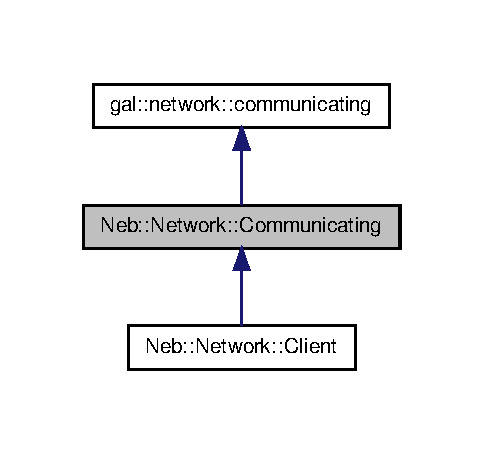
\includegraphics[width=232pt]{classNeb_1_1Network_1_1Communicating__inherit__graph}
\end{center}
\end{figure}


\-Collaboration diagram for \-Neb\-:\-:\-Network\-:\-:\-Communicating\-:\nopagebreak
\begin{figure}[H]
\begin{center}
\leavevmode
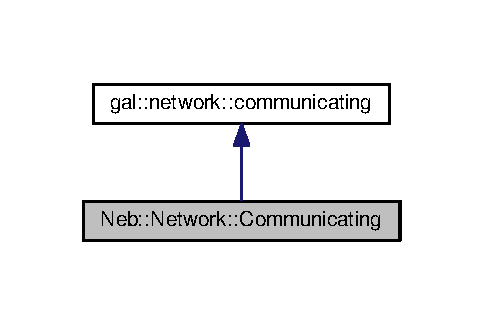
\includegraphics[width=232pt]{classNeb_1_1Network_1_1Communicating__coll__graph}
\end{center}
\end{figure}
\subsection*{\-Public \-Member \-Functions}
\begin{DoxyCompactItemize}
\item 
\hypertarget{classNeb_1_1Network_1_1Communicating_a49209dffa98203430d9c27d06bf2f20e}{{\bfseries \-Communicating} (int)}\label{classNeb_1_1Network_1_1Communicating_a49209dffa98203430d9c27d06bf2f20e}

\item 
\hypertarget{classNeb_1_1Network_1_1Communicating_accb7cece4006dabcb09bea96bd728175}{void {\bfseries process} (gal\-::network\-::message\-\_\-s)}\label{classNeb_1_1Network_1_1Communicating_accb7cece4006dabcb09bea96bd728175}

\end{DoxyCompactItemize}


\-The documentation for this class was generated from the following file\-:\begin{DoxyCompactItemize}
\item 
src/\-Nebula/network2/communicating.\-hh\end{DoxyCompactItemize}

\hypertarget{classNeb_1_1Actor_1_1Controller}{\section{\-Neb\-:\-:\-Actor\-:\-:\-Controller \-Class \-Reference}
\label{classNeb_1_1Actor_1_1Controller}\index{\-Neb\-::\-Actor\-::\-Controller@{\-Neb\-::\-Actor\-::\-Controller}}
}


\-Inheritance diagram for \-Neb\-:\-:\-Actor\-:\-:\-Controller\-:
\nopagebreak
\begin{figure}[H]
\begin{center}
\leavevmode
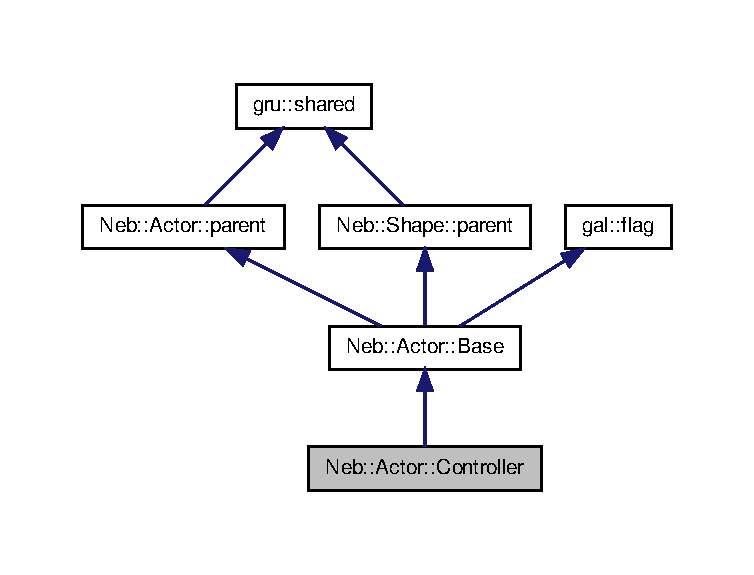
\includegraphics[width=350pt]{classNeb_1_1Actor_1_1Controller__inherit__graph}
\end{center}
\end{figure}


\-Collaboration diagram for \-Neb\-:\-:\-Actor\-:\-:\-Controller\-:
\nopagebreak
\begin{figure}[H]
\begin{center}
\leavevmode
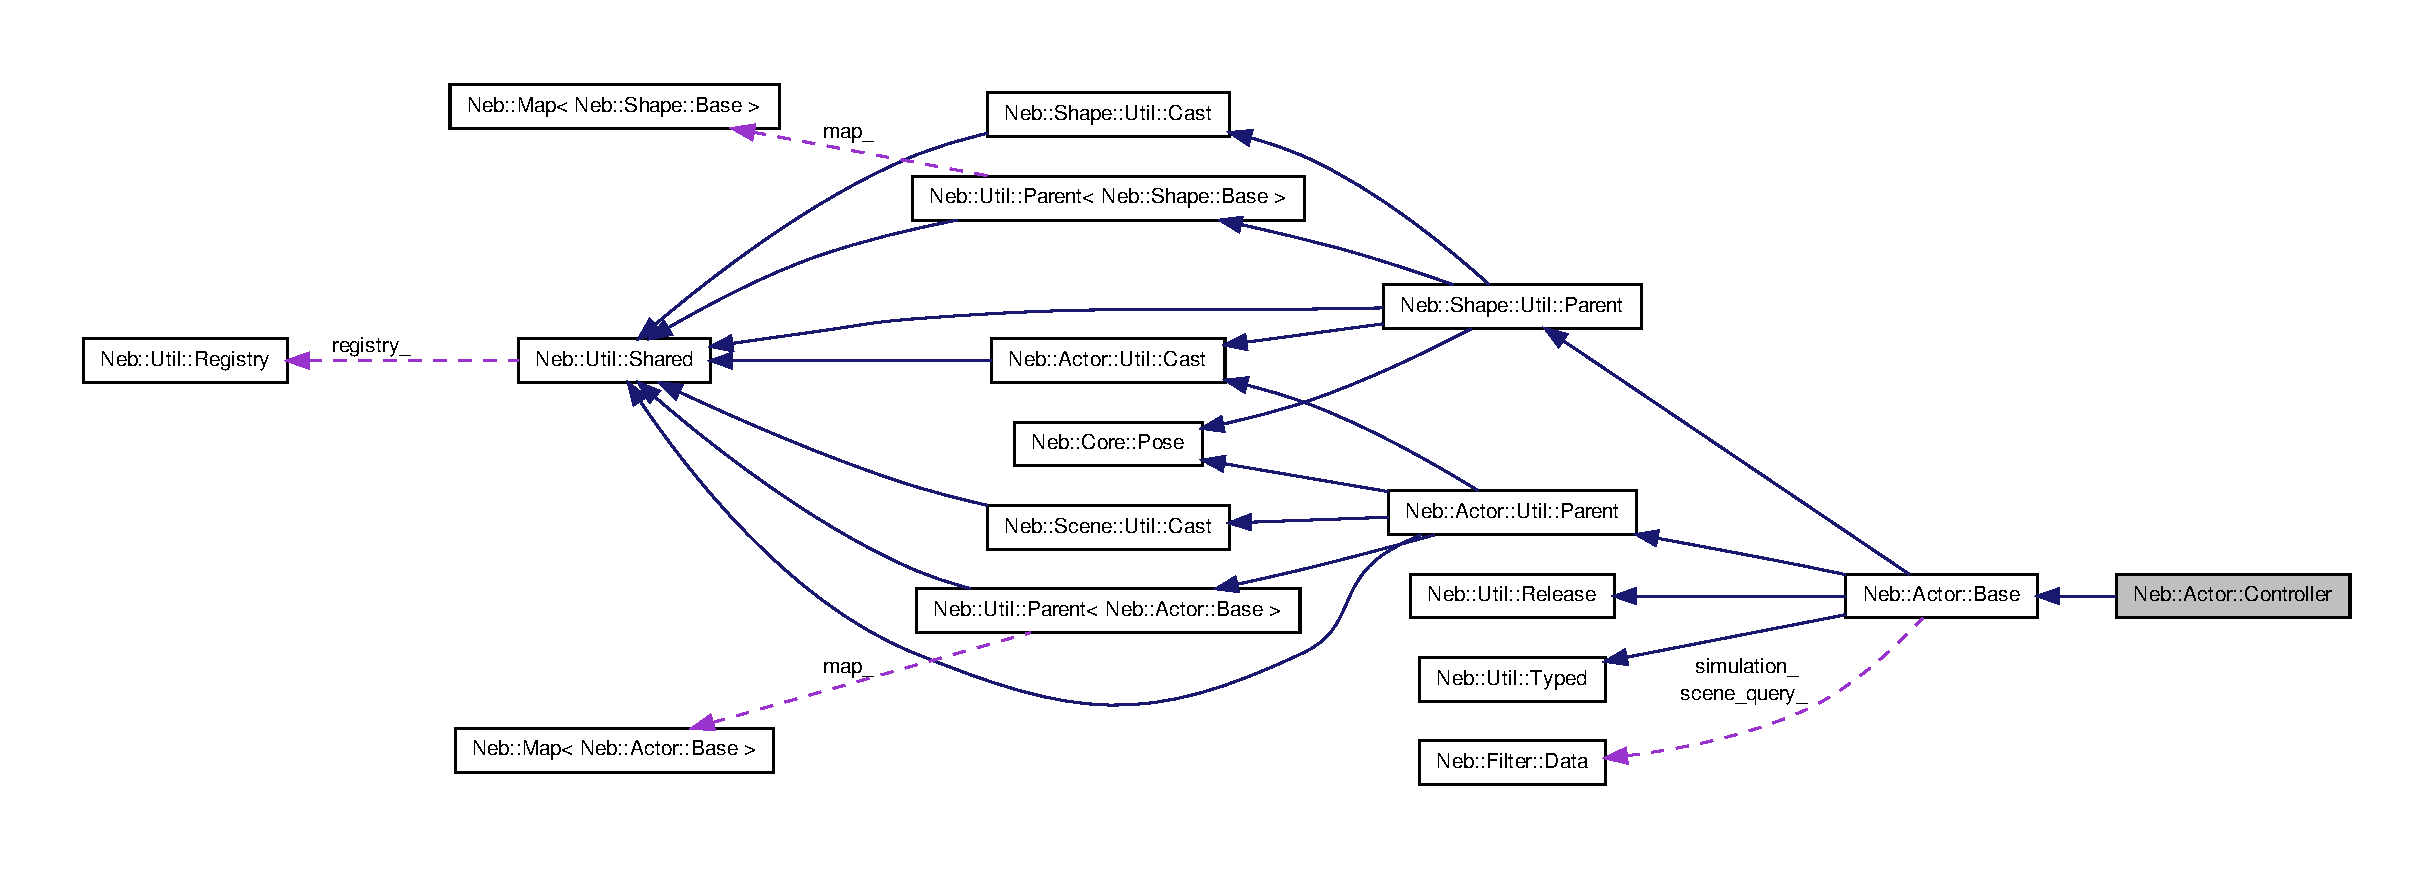
\includegraphics[width=350pt]{classNeb_1_1Actor_1_1Controller__coll__graph}
\end{center}
\end{figure}
\subsection*{\-Public \-Member \-Functions}
\begin{DoxyCompactItemize}
\item 
\hypertarget{classNeb_1_1Actor_1_1Controller_ac872fdf65f915761b1aed60ca8a835de}{{\bfseries \-Controller} (\hyperlink{classNeb_1_1weak__ptr}{\-Neb\-::weak\-\_\-ptr}$<$ \hyperlink{classNeb_1_1Actor_1_1parent}{\-Neb\-::\-Actor\-::parent} $>$)}\label{classNeb_1_1Actor_1_1Controller_ac872fdf65f915761b1aed60ca8a835de}

\item 
\hypertarget{classNeb_1_1Actor_1_1Controller_a4cf7cbd70138ea33c509d89ebc74e45d}{virtual void {\bfseries release} ()}\label{classNeb_1_1Actor_1_1Controller_a4cf7cbd70138ea33c509d89ebc74e45d}

\item 
\hypertarget{classNeb_1_1Actor_1_1Controller_a37d671a837e578ee05e2f9e1a5292e79}{virtual void {\bfseries step} (float)}\label{classNeb_1_1Actor_1_1Controller_a37d671a837e578ee05e2f9e1a5292e79}

\item 
\hypertarget{classNeb_1_1Actor_1_1Controller_abd3a89e2acfc654033cd70bbec7491a6}{virtual void {\bfseries init} (\hyperlink{classNeb_1_1weak__ptr}{\-Neb\-::\-Actor\-::desc\-\_\-w})}\label{classNeb_1_1Actor_1_1Controller_abd3a89e2acfc654033cd70bbec7491a6}

\item 
\hypertarget{classNeb_1_1Actor_1_1Controller_aed64790b9ac840ebb4e6da3af3a6e405}{virtual void {\bfseries add\-\_\-force} ()}\label{classNeb_1_1Actor_1_1Controller_aed64790b9ac840ebb4e6da3af3a6e405}

\end{DoxyCompactItemize}
\subsection*{\-Public \-Attributes}
\begin{DoxyCompactItemize}
\item 
\hypertarget{classNeb_1_1Actor_1_1Controller_a488fba03acad68f997a3f38f4fac41fd}{physx\-::\-Px\-Controller $\ast$ {\bfseries px\-\_\-controller\-\_\-}}\label{classNeb_1_1Actor_1_1Controller_a488fba03acad68f997a3f38f4fac41fd}

\end{DoxyCompactItemize}


\-The documentation for this class was generated from the following files\-:\begin{DoxyCompactItemize}
\item 
src/\-Nebula/\-Actor/\-Controller.\-hpp\item 
src/\-Nebula/\-Actor/\-Controller.\-cpp\end{DoxyCompactItemize}

\hypertarget{structNeb_1_1Message_1_1Scene_1_1Create}{\section{\-Neb\-:\-:\-Message\-:\-:\-Scene\-:\-:\-Create \-Struct \-Reference}
\label{structNeb_1_1Message_1_1Scene_1_1Create}\index{\-Neb\-::\-Message\-::\-Scene\-::\-Create@{\-Neb\-::\-Message\-::\-Scene\-::\-Create}}
}


\-Collaboration diagram for \-Neb\-:\-:\-Message\-:\-:\-Scene\-:\-:\-Create\-:\nopagebreak
\begin{figure}[H]
\begin{center}
\leavevmode
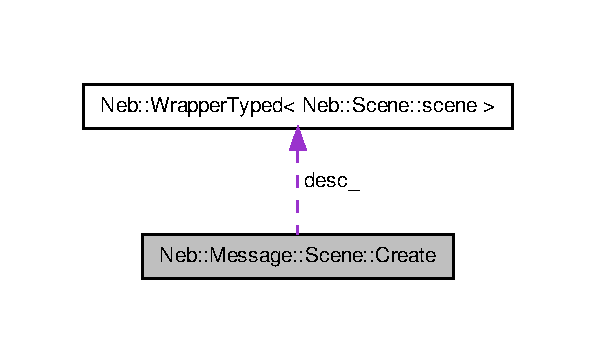
\includegraphics[width=286pt]{structNeb_1_1Message_1_1Scene_1_1Create__coll__graph}
\end{center}
\end{figure}
\subsection*{\-Public \-Member \-Functions}
\begin{DoxyCompactItemize}
\item 
\hypertarget{structNeb_1_1Message_1_1Scene_1_1Create_a2550a95749cbd9ae2e8fcef05bf53025}{void {\bfseries load} (\hyperlink{classNeb_1_1weak__ptr}{\-Neb\-::weak\-\_\-ptr}$<$ glutpp\-::scene\-::scene $>$ scene)}\label{structNeb_1_1Message_1_1Scene_1_1Create_a2550a95749cbd9ae2e8fcef05bf53025}

\item 
\hypertarget{structNeb_1_1Message_1_1Scene_1_1Create_ab128d0e116d07b1034ef8f25adcfa4ac}{{\footnotesize template$<$class Archive $>$ }\\void {\bfseries serialize} (\-Archive \&ar, unsigned int const \&version)}\label{structNeb_1_1Message_1_1Scene_1_1Create_ab128d0e116d07b1034ef8f25adcfa4ac}

\end{DoxyCompactItemize}
\subsection*{\-Public \-Attributes}
\begin{DoxyCompactItemize}
\item 
\hypertarget{structNeb_1_1Message_1_1Scene_1_1Create_a96b31f22acdda789448875a3c41b3cba}{glutpp\-::scene\-::addr {\bfseries addr\-\_\-}}\label{structNeb_1_1Message_1_1Scene_1_1Create_a96b31f22acdda789448875a3c41b3cba}

\item 
\hypertarget{structNeb_1_1Message_1_1Scene_1_1Create_a2859067240bab51b1afd65055713888a}{\hyperlink{classNeb_1_1WrapperTyped}{\-Neb\-::\-Wrapper\-Typed}\*
$<$ \-Neb\-::\-Scene\-::scene $>$ {\bfseries desc\-\_\-}}\label{structNeb_1_1Message_1_1Scene_1_1Create_a2859067240bab51b1afd65055713888a}

\end{DoxyCompactItemize}


\-The documentation for this struct was generated from the following file\-:\begin{DoxyCompactItemize}
\item 
src/\-Nebula/\-Message/\-Scene/\-Create.\-hpp\end{DoxyCompactItemize}

\hypertarget{classNeb_1_1Message_1_1Actor_1_1Control_1_1RigidBody_1_1Create}{\section{\-Neb\-:\-:\-Message\-:\-:\-Actor\-:\-:\-Control\-:\-:\-Rigid\-Body\-:\-:\-Create \-Class \-Reference}
\label{classNeb_1_1Message_1_1Actor_1_1Control_1_1RigidBody_1_1Create}\index{\-Neb\-::\-Message\-::\-Actor\-::\-Control\-::\-Rigid\-Body\-::\-Create@{\-Neb\-::\-Message\-::\-Actor\-::\-Control\-::\-Rigid\-Body\-::\-Create}}
}


\-Create.  




{\ttfamily \#include $<$\-Control.\-hh$>$}



\-Inheritance diagram for \-Neb\-:\-:\-Message\-:\-:\-Actor\-:\-:\-Control\-:\-:\-Rigid\-Body\-:\-:\-Create\-:\nopagebreak
\begin{figure}[H]
\begin{center}
\leavevmode
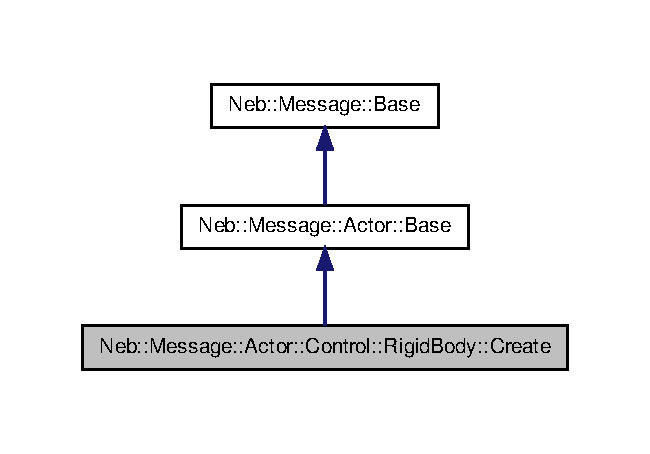
\includegraphics[width=312pt]{classNeb_1_1Message_1_1Actor_1_1Control_1_1RigidBody_1_1Create__inherit__graph}
\end{center}
\end{figure}


\-Collaboration diagram for \-Neb\-:\-:\-Message\-:\-:\-Actor\-:\-:\-Control\-:\-:\-Rigid\-Body\-:\-:\-Create\-:\nopagebreak
\begin{figure}[H]
\begin{center}
\leavevmode
\includegraphics[width=350pt]{classNeb_1_1Message_1_1Actor_1_1Control_1_1RigidBody_1_1Create__coll__graph}
\end{center}
\end{figure}
\subsection*{\-Public \-Member \-Functions}
\begin{DoxyCompactItemize}
\item 
\hypertarget{classNeb_1_1Message_1_1Actor_1_1Control_1_1RigidBody_1_1Create_acbf4c5b3ac614c8d23c24eebd5c0c262}{virtual void \hyperlink{classNeb_1_1Message_1_1Actor_1_1Control_1_1RigidBody_1_1Create_acbf4c5b3ac614c8d23c24eebd5c0c262}{serialize\-Derived} (boost\-::archive\-::polymorphic\-\_\-oarchive \&ar, unsigned int const \&version)}\label{classNeb_1_1Message_1_1Actor_1_1Control_1_1RigidBody_1_1Create_acbf4c5b3ac614c8d23c24eebd5c0c262}

\begin{DoxyCompactList}\small\item\em derived serialize. \end{DoxyCompactList}\item 
\hypertarget{classNeb_1_1Message_1_1Actor_1_1Control_1_1RigidBody_1_1Create_a605672877b5e29fa8a4b400de203e83f}{virtual void \hyperlink{classNeb_1_1Message_1_1Actor_1_1Control_1_1RigidBody_1_1Create_a605672877b5e29fa8a4b400de203e83f}{serialize\-Derived} (boost\-::archive\-::polymorphic\-\_\-iarchive \&ar, unsigned int const \&version)}\label{classNeb_1_1Message_1_1Actor_1_1Control_1_1RigidBody_1_1Create_a605672877b5e29fa8a4b400de203e83f}

\begin{DoxyCompactList}\small\item\em derived serialize. \end{DoxyCompactList}\end{DoxyCompactItemize}
\subsection*{\-Public \-Attributes}
\begin{DoxyCompactItemize}
\item 
\hypertarget{classNeb_1_1Message_1_1Actor_1_1Control_1_1RigidBody_1_1Create_ad5dad4e62045e21146c253792c0c36ee}{\hyperlink{classNeb_1_1WrapperTyped}{\-Neb\-::\-Wrapper\-Typed}\*
$<$ \hyperlink{classNeb_1_1Actor_1_1Control_1_1RigidBody_1_1Base}{\-Neb\-::\-Actor\-::\-Control\-::\-Rigid\-Body\-::\-Base} $>$ {\bfseries control\-\_\-}}\label{classNeb_1_1Message_1_1Actor_1_1Control_1_1RigidBody_1_1Create_ad5dad4e62045e21146c253792c0c36ee}

\end{DoxyCompactItemize}


\subsection{\-Detailed \-Description}
\-Create. 

\-The documentation for this class was generated from the following file\-:\begin{DoxyCompactItemize}
\item 
src/\-Nebula/\-Message/\-Actor/\-Control.\-hh\end{DoxyCompactItemize}

\hypertarget{structNeb_1_1Message_1_1Actor_1_1Create}{\section{Neb\-:\-:Message\-:\-:Actor\-:\-:Create Struct Reference}
\label{structNeb_1_1Message_1_1Actor_1_1Create}\index{Neb\-::\-Message\-::\-Actor\-::\-Create@{Neb\-::\-Message\-::\-Actor\-::\-Create}}
}


Collaboration diagram for Neb\-:\-:Message\-:\-:Actor\-:\-:Create\-:
\nopagebreak
\begin{figure}[H]
\begin{center}
\leavevmode
\includegraphics[width=216pt]{structNeb_1_1Message_1_1Actor_1_1Create__coll__graph}
\end{center}
\end{figure}
\subsection*{Public Member Functions}
\begin{DoxyCompactItemize}
\item 
\hypertarget{structNeb_1_1Message_1_1Actor_1_1Create_aff6ea433625795e13837dadbf4c36bca}{void {\bfseries load} (Neb\-::actor\-::actor\-\_\-w actor)}\label{structNeb_1_1Message_1_1Actor_1_1Create_aff6ea433625795e13837dadbf4c36bca}

\item 
\hypertarget{structNeb_1_1Message_1_1Actor_1_1Create_a4805dfe7cf6d556732278330dd7f7c44}{{\footnotesize template$<$class Archive $>$ }\\void {\bfseries serialize} (Archive \&ar, unsigned int const \&version)}\label{structNeb_1_1Message_1_1Actor_1_1Create_a4805dfe7cf6d556732278330dd7f7c44}

\end{DoxyCompactItemize}
\subsection*{Public Attributes}
\begin{DoxyCompactItemize}
\item 
\hypertarget{structNeb_1_1Message_1_1Actor_1_1Create_a925e9660c46a4264a84fdaad5dc79da8}{Neb\-::\-Actor\-::addr \hyperlink{structNeb_1_1Message_1_1Actor_1_1Create_a925e9660c46a4264a84fdaad5dc79da8}{addr\-\_\-}}\label{structNeb_1_1Message_1_1Actor_1_1Create_a925e9660c46a4264a84fdaad5dc79da8}

\begin{DoxyCompactList}\small\item\em Address. address at which the new actor object will be stored. \end{DoxyCompactList}\item 
\hypertarget{structNeb_1_1Message_1_1Actor_1_1Create_a6aae87ea763a64722094752017a9ba9b}{\hyperlink{classNeb_1_1WrapperTyped}{Neb\-::\-Wrapper\-Typed}\\*
$<$ \hyperlink{classNeb_1_1Actor_1_1Base}{Neb\-::\-Actor\-::\-Base} $>$ \hyperlink{structNeb_1_1Message_1_1Actor_1_1Create_a6aae87ea763a64722094752017a9ba9b}{wrapper\-\_\-}}\label{structNeb_1_1Message_1_1Actor_1_1Create_a6aae87ea763a64722094752017a9ba9b}

\begin{DoxyCompactList}\small\item\em Wrapper. wrapper to create the actor object. \end{DoxyCompactList}\end{DoxyCompactItemize}


The documentation for this struct was generated from the following file\-:\begin{DoxyCompactItemize}
\item 
src/\-Nebula/\-Message/\-Actor/Create.\-hh\end{DoxyCompactItemize}

\hypertarget{classmath_1_1geo_1_1cuboid}{\section{math\-:\-:geo\-:\-:cuboid \-Class \-Reference}
\label{classmath_1_1geo_1_1cuboid}\index{math\-::geo\-::cuboid@{math\-::geo\-::cuboid}}
}


\-Inheritance diagram for math\-:\-:geo\-:\-:cuboid\-:
\nopagebreak
\begin{figure}[H]
\begin{center}
\leavevmode
\includegraphics[width=230pt]{classmath_1_1geo_1_1cuboid__inherit__graph}
\end{center}
\end{figure}


\-Collaboration diagram for math\-:\-:geo\-:\-:cuboid\-:
\nopagebreak
\begin{figure}[H]
\begin{center}
\leavevmode
\includegraphics[width=314pt]{classmath_1_1geo_1_1cuboid__coll__graph}
\end{center}
\end{figure}
\subsection*{\-Public \-Member \-Functions}
\begin{DoxyCompactItemize}
\item 
\hypertarget{classmath_1_1geo_1_1cuboid_a72bd7e6bf32ccd6928e375efa3036491}{{\bfseries cuboid} (float, float, float)}\label{classmath_1_1geo_1_1cuboid_a72bd7e6bf32ccd6928e375efa3036491}

\end{DoxyCompactItemize}


\-The documentation for this class was generated from the following file\-:\begin{DoxyCompactItemize}
\item 
src/gru/\-Math/geo/polyhedron.\-hpp\end{DoxyCompactItemize}

\hypertarget{classNeb_1_1gui_1_1object_1_1Data}{\section{\-Neb\-:\-:gui\-:\-:object\-:\-:\-Data \-Class \-Reference}
\label{classNeb_1_1gui_1_1object_1_1Data}\index{\-Neb\-::gui\-::object\-::\-Data@{\-Neb\-::gui\-::object\-::\-Data}}
}


\-Collaboration diagram for \-Neb\-:\-:gui\-:\-:object\-:\-:\-Data\-:\nopagebreak
\begin{figure}[H]
\begin{center}
\leavevmode
\includegraphics[width=208pt]{classNeb_1_1gui_1_1object_1_1Data__coll__graph}
\end{center}
\end{figure}
\subsection*{\-Public \-Member \-Functions}
\begin{DoxyCompactItemize}
\item 
\hypertarget{classNeb_1_1gui_1_1object_1_1Data_acb81238a3d1971c883a1136c4ac53bc0}{{\footnotesize template$<$class Archive $>$ }\\void {\bfseries serialize} (\-Archive \&ar, unsigned int const \&version)}\label{classNeb_1_1gui_1_1object_1_1Data_acb81238a3d1971c883a1136c4ac53bc0}

\end{DoxyCompactItemize}
\subsection*{\-Public \-Attributes}
\begin{DoxyCompactItemize}
\item 
\hypertarget{classNeb_1_1gui_1_1object_1_1Data_a7273b450412527b0ee04a2508dd05cce}{float {\bfseries x\-\_\-}}\label{classNeb_1_1gui_1_1object_1_1Data_a7273b450412527b0ee04a2508dd05cce}

\item 
\hypertarget{classNeb_1_1gui_1_1object_1_1Data_ada3026fdd107ddbe43a6de6430418901}{float {\bfseries y\-\_\-}}\label{classNeb_1_1gui_1_1object_1_1Data_ada3026fdd107ddbe43a6de6430418901}

\item 
\hypertarget{classNeb_1_1gui_1_1object_1_1Data_a174449b7b4c88c25d19efe06f022e4b7}{float {\bfseries w\-\_\-}}\label{classNeb_1_1gui_1_1object_1_1Data_a174449b7b4c88c25d19efe06f022e4b7}

\item 
\hypertarget{classNeb_1_1gui_1_1object_1_1Data_aba2bfb2f1819f911595e4e52ef2c761c}{float {\bfseries h\-\_\-}}\label{classNeb_1_1gui_1_1object_1_1Data_aba2bfb2f1819f911595e4e52ef2c761c}

\item 
\hypertarget{classNeb_1_1gui_1_1object_1_1Data_a03ed3fa05b542d10e31322ee627a40f4}{\hyperlink{classNeb_1_1Color_1_1color}{\-Neb\-::\-Color\-::color}$<$ float $>$ {\bfseries font\-\_\-color\-\_\-}}\label{classNeb_1_1gui_1_1object_1_1Data_a03ed3fa05b542d10e31322ee627a40f4}

\item 
\hypertarget{classNeb_1_1gui_1_1object_1_1Data_a097b47c78cc539d75e1a895a2a385748}{\hyperlink{classNeb_1_1Color_1_1color}{\-Neb\-::\-Color\-::color}$<$ float $>$ {\bfseries bg\-\_\-color\-\_\-}}\label{classNeb_1_1gui_1_1object_1_1Data_a097b47c78cc539d75e1a895a2a385748}

\item 
\hypertarget{classNeb_1_1gui_1_1object_1_1Data_a36135fece215ee3a34ca8f11e67b5b72}{std\-::string {\bfseries label\-\_\-}}\label{classNeb_1_1gui_1_1object_1_1Data_a36135fece215ee3a34ca8f11e67b5b72}

\end{DoxyCompactItemize}


\-The documentation for this class was generated from the following files\-:\begin{DoxyCompactItemize}
\item 
src/\-Nebula/\-Graphics/gui/object/object.\-hpp\item 
src/\-Nebula/\-Graphics/gui/object/object.\-cpp\end{DoxyCompactItemize}

\hypertarget{classNeb_1_1Filter_1_1Data}{\section{\-Neb\-:\-:\-Filter\-:\-:\-Data \-Class \-Reference}
\label{classNeb_1_1Filter_1_1Data}\index{\-Neb\-::\-Filter\-::\-Data@{\-Neb\-::\-Filter\-::\-Data}}
}
\subsection*{\-Public \-Member \-Functions}
\begin{DoxyCompactItemize}
\item 
\hypertarget{classNeb_1_1Filter_1_1Data_a727a2c1fa8011f050ada6e871230b585}{{\footnotesize template$<$class Archive $>$ }\\void {\bfseries serialize} (\-Archive \&ar, unsigned int const \&version)}\label{classNeb_1_1Filter_1_1Data_a727a2c1fa8011f050ada6e871230b585}

\end{DoxyCompactItemize}
\subsection*{\-Public \-Attributes}
\begin{DoxyCompactItemize}
\item 
\hypertarget{classNeb_1_1Filter_1_1Data_a4c58a7b73274baec2618f3aaa658737e}{unsigned int {\bfseries word0}}\label{classNeb_1_1Filter_1_1Data_a4c58a7b73274baec2618f3aaa658737e}

\item 
\hypertarget{classNeb_1_1Filter_1_1Data_a53392967cf835071bf2bb34fa96dcf1c}{unsigned int {\bfseries word1}}\label{classNeb_1_1Filter_1_1Data_a53392967cf835071bf2bb34fa96dcf1c}

\item 
\hypertarget{classNeb_1_1Filter_1_1Data_a32ac663d2a72a3c1f3e97dd329c0db5c}{unsigned int {\bfseries word2}}\label{classNeb_1_1Filter_1_1Data_a32ac663d2a72a3c1f3e97dd329c0db5c}

\item 
\hypertarget{classNeb_1_1Filter_1_1Data_a5e0caefa84858430a4456fcd381cb537}{unsigned int {\bfseries word3}}\label{classNeb_1_1Filter_1_1Data_a5e0caefa84858430a4456fcd381cb537}

\end{DoxyCompactItemize}


\-The documentation for this class was generated from the following file\-:\begin{DoxyCompactItemize}
\item 
src/\-Nebula/\-Filter.\-hpp\end{DoxyCompactItemize}

\hypertarget{classDefaultErrorCallback}{\section{\-Default\-Error\-Callback \-Class \-Reference}
\label{classDefaultErrorCallback}\index{\-Default\-Error\-Callback@{\-Default\-Error\-Callback}}
}
\subsection*{\-Public \-Member \-Functions}
\begin{DoxyCompactItemize}
\item 
\hypertarget{classDefaultErrorCallback_ae95118f6a45b47a1b72af9417f80d84e}{void {\bfseries report\-Error} (physx\-::\-Px\-Error\-Code\-::\-Enum code, char const $\ast$message, char const $\ast$file, int line)}\label{classDefaultErrorCallback_ae95118f6a45b47a1b72af9417f80d84e}

\end{DoxyCompactItemize}


\-The documentation for this class was generated from the following files\-:\begin{DoxyCompactItemize}
\item 
src/nebula/physics.\-hpp\item 
src/nebula/physics.\-cpp\end{DoxyCompactItemize}

\hypertarget{classNeb_1_1Light_1_1Directional}{\section{\-Neb\-:\-:\-Light\-:\-:\-Directional \-Class \-Reference}
\label{classNeb_1_1Light_1_1Directional}\index{\-Neb\-::\-Light\-::\-Directional@{\-Neb\-::\-Light\-::\-Directional}}
}


\-Inheritance diagram for \-Neb\-:\-:\-Light\-:\-:\-Directional\-:\nopagebreak
\begin{figure}[H]
\begin{center}
\leavevmode
\includegraphics[width=194pt]{classNeb_1_1Light_1_1Directional__inherit__graph}
\end{center}
\end{figure}


\-Collaboration diagram for \-Neb\-:\-:\-Light\-:\-:\-Directional\-:\nopagebreak
\begin{figure}[H]
\begin{center}
\leavevmode
\includegraphics[width=350pt]{classNeb_1_1Light_1_1Directional__coll__graph}
\end{center}
\end{figure}


\-The documentation for this class was generated from the following file\-:\begin{DoxyCompactItemize}
\item 
src/\-Nebula/\-Graphics/\-Light/\-Spot.\-hh\end{DoxyCompactItemize}

\hypertarget{classNeb_1_1glsl_1_1Uniform_1_1Scalar_1_1Double}{\section{\-Neb\-:\-:glsl\-:\-:\-Uniform\-:\-:\-Scalar\-:\-:\-Double \-Class \-Reference}
\label{classNeb_1_1glsl_1_1Uniform_1_1Scalar_1_1Double}\index{\-Neb\-::glsl\-::\-Uniform\-::\-Scalar\-::\-Double@{\-Neb\-::glsl\-::\-Uniform\-::\-Scalar\-::\-Double}}
}


\-Inheritance diagram for \-Neb\-:\-:glsl\-:\-:\-Uniform\-:\-:\-Scalar\-:\-:\-Double\-:\nopagebreak
\begin{figure}[H]
\begin{center}
\leavevmode
\includegraphics[width=246pt]{classNeb_1_1glsl_1_1Uniform_1_1Scalar_1_1Double__inherit__graph}
\end{center}
\end{figure}


\-Collaboration diagram for \-Neb\-:\-:glsl\-:\-:\-Uniform\-:\-:\-Scalar\-:\-:\-Double\-:\nopagebreak
\begin{figure}[H]
\begin{center}
\leavevmode
\includegraphics[width=246pt]{classNeb_1_1glsl_1_1Uniform_1_1Scalar_1_1Double__coll__graph}
\end{center}
\end{figure}
\subsection*{\-Public \-Member \-Functions}
\begin{DoxyCompactItemize}
\item 
\hypertarget{classNeb_1_1glsl_1_1Uniform_1_1Scalar_1_1Double_a69bb07fb2fa171a1067bf7558b91ec57}{{\bfseries \-Double} (std\-::string s)}\label{classNeb_1_1glsl_1_1Uniform_1_1Scalar_1_1Double_a69bb07fb2fa171a1067bf7558b91ec57}

\item 
\hypertarget{classNeb_1_1glsl_1_1Uniform_1_1Scalar_1_1Double_aa3e09a61118c65d3af510b3f7b8080ec}{virtual void {\bfseries load} (double)}\label{classNeb_1_1glsl_1_1Uniform_1_1Scalar_1_1Double_aa3e09a61118c65d3af510b3f7b8080ec}

\end{DoxyCompactItemize}


\-The documentation for this class was generated from the following files\-:\begin{DoxyCompactItemize}
\item 
src/\-Nebula/\-Graphics/glsl/\-Uniform/uniform.\-hh\item 
src/\-Nebula/\-Graphics/glsl/\-Uniform/\-Float.\-cc\end{DoxyCompactItemize}

\hypertarget{classNeb_1_1glsl_1_1Uniform_1_1Vector_1_1Double}{\section{\-Neb\-:\-:glsl\-:\-:\-Uniform\-:\-:\-Vector\-:\-:\-Double \-Class \-Reference}
\label{classNeb_1_1glsl_1_1Uniform_1_1Vector_1_1Double}\index{\-Neb\-::glsl\-::\-Uniform\-::\-Vector\-::\-Double@{\-Neb\-::glsl\-::\-Uniform\-::\-Vector\-::\-Double}}
}


\-Inheritance diagram for \-Neb\-:\-:glsl\-:\-:\-Uniform\-:\-:\-Vector\-:\-:\-Double\-:\nopagebreak
\begin{figure}[H]
\begin{center}
\leavevmode
\includegraphics[width=246pt]{classNeb_1_1glsl_1_1Uniform_1_1Vector_1_1Double__inherit__graph}
\end{center}
\end{figure}


\-Collaboration diagram for \-Neb\-:\-:glsl\-:\-:\-Uniform\-:\-:\-Vector\-:\-:\-Double\-:\nopagebreak
\begin{figure}[H]
\begin{center}
\leavevmode
\includegraphics[width=246pt]{classNeb_1_1glsl_1_1Uniform_1_1Vector_1_1Double__coll__graph}
\end{center}
\end{figure}
\subsection*{\-Public \-Member \-Functions}
\begin{DoxyCompactItemize}
\item 
\hypertarget{classNeb_1_1glsl_1_1Uniform_1_1Vector_1_1Double_a4f5b3ffeff4c2d183a7af7401c434731}{{\bfseries \-Double} (std\-::string s1, std\-::string s2)}\label{classNeb_1_1glsl_1_1Uniform_1_1Vector_1_1Double_a4f5b3ffeff4c2d183a7af7401c434731}

\item 
\hypertarget{classNeb_1_1glsl_1_1Uniform_1_1Vector_1_1Double_a8e4ae1631ba13b00afede31a82d91481}{virtual void {\bfseries load} (int, double)}\label{classNeb_1_1glsl_1_1Uniform_1_1Vector_1_1Double_a8e4ae1631ba13b00afede31a82d91481}

\end{DoxyCompactItemize}


\-The documentation for this class was generated from the following file\-:\begin{DoxyCompactItemize}
\item 
src/\-Nebula/\-Graphics/glsl/\-Uniform/uniform.\-hpp\end{DoxyCompactItemize}

\hypertarget{classNeb_1_1glsl_1_1Uniform_1_1Vector_1_1DVec3}{\section{\-Neb\-:\-:glsl\-:\-:\-Uniform\-:\-:\-Vector\-:\-:\-D\-Vec3 \-Class \-Reference}
\label{classNeb_1_1glsl_1_1Uniform_1_1Vector_1_1DVec3}\index{\-Neb\-::glsl\-::\-Uniform\-::\-Vector\-::\-D\-Vec3@{\-Neb\-::glsl\-::\-Uniform\-::\-Vector\-::\-D\-Vec3}}
}


\-Inheritance diagram for \-Neb\-:\-:glsl\-:\-:\-Uniform\-:\-:\-Vector\-:\-:\-D\-Vec3\-:\nopagebreak
\begin{figure}[H]
\begin{center}
\leavevmode
\includegraphics[width=246pt]{classNeb_1_1glsl_1_1Uniform_1_1Vector_1_1DVec3__inherit__graph}
\end{center}
\end{figure}


\-Collaboration diagram for \-Neb\-:\-:glsl\-:\-:\-Uniform\-:\-:\-Vector\-:\-:\-D\-Vec3\-:\nopagebreak
\begin{figure}[H]
\begin{center}
\leavevmode
\includegraphics[width=246pt]{classNeb_1_1glsl_1_1Uniform_1_1Vector_1_1DVec3__coll__graph}
\end{center}
\end{figure}
\subsection*{\-Public \-Member \-Functions}
\begin{DoxyCompactItemize}
\item 
\hypertarget{classNeb_1_1glsl_1_1Uniform_1_1Vector_1_1DVec3_a0eafe586b49fbf3f40483014ee8ab93d}{{\bfseries \-D\-Vec3} (std\-::string s1, std\-::string s2)}\label{classNeb_1_1glsl_1_1Uniform_1_1Vector_1_1DVec3_a0eafe586b49fbf3f40483014ee8ab93d}

\item 
\hypertarget{classNeb_1_1glsl_1_1Uniform_1_1Vector_1_1DVec3_a259ae2290abc4445a5c661d2547597b5}{virtual void {\bfseries load} (int, double $\ast$)}\label{classNeb_1_1glsl_1_1Uniform_1_1Vector_1_1DVec3_a259ae2290abc4445a5c661d2547597b5}

\end{DoxyCompactItemize}


\-The documentation for this class was generated from the following file\-:\begin{DoxyCompactItemize}
\item 
src/\-Nebula/\-Graphics/glsl/\-Uniform/uniform.\-hh\end{DoxyCompactItemize}

\hypertarget{classNeb_1_1glsl_1_1Uniform_1_1Scalar_1_1DVec4}{\section{Neb\-:\-:glsl\-:\-:Uniform\-:\-:Scalar\-:\-:D\-Vec4 Class Reference}
\label{classNeb_1_1glsl_1_1Uniform_1_1Scalar_1_1DVec4}\index{Neb\-::glsl\-::\-Uniform\-::\-Scalar\-::\-D\-Vec4@{Neb\-::glsl\-::\-Uniform\-::\-Scalar\-::\-D\-Vec4}}
}


Inheritance diagram for Neb\-:\-:glsl\-:\-:Uniform\-:\-:Scalar\-:\-:D\-Vec4\-:
\nopagebreak
\begin{figure}[H]
\begin{center}
\leavevmode
\includegraphics[width=176pt]{classNeb_1_1glsl_1_1Uniform_1_1Scalar_1_1DVec4__inherit__graph}
\end{center}
\end{figure}


Collaboration diagram for Neb\-:\-:glsl\-:\-:Uniform\-:\-:Scalar\-:\-:D\-Vec4\-:
\nopagebreak
\begin{figure}[H]
\begin{center}
\leavevmode
\includegraphics[width=176pt]{classNeb_1_1glsl_1_1Uniform_1_1Scalar_1_1DVec4__coll__graph}
\end{center}
\end{figure}
\subsection*{Public Member Functions}
\begin{DoxyCompactItemize}
\item 
\hypertarget{classNeb_1_1glsl_1_1Uniform_1_1Scalar_1_1DVec4_ab8470910b7562c6a60cb01270b1fa028}{{\bfseries D\-Vec4} (std\-::string s)}\label{classNeb_1_1glsl_1_1Uniform_1_1Scalar_1_1DVec4_ab8470910b7562c6a60cb01270b1fa028}

\item 
\hypertarget{classNeb_1_1glsl_1_1Uniform_1_1Scalar_1_1DVec4_af843bf42042cbe62f8744a1621ef4178}{virtual void {\bfseries load} (double $\ast$)}\label{classNeb_1_1glsl_1_1Uniform_1_1Scalar_1_1DVec4_af843bf42042cbe62f8744a1621ef4178}

\end{DoxyCompactItemize}
\subsection*{Additional Inherited Members}


The documentation for this class was generated from the following file\-:\begin{DoxyCompactItemize}
\item 
src/\-Nebula/\-Graphics/glsl/\-Uniform/uniform.\-hh\end{DoxyCompactItemize}

\hypertarget{classNeb_1_1glsl_1_1Uniform_1_1Vector_1_1DVec4}{\section{\-Neb\-:\-:glsl\-:\-:\-Uniform\-:\-:\-Vector\-:\-:\-D\-Vec4 \-Class \-Reference}
\label{classNeb_1_1glsl_1_1Uniform_1_1Vector_1_1DVec4}\index{\-Neb\-::glsl\-::\-Uniform\-::\-Vector\-::\-D\-Vec4@{\-Neb\-::glsl\-::\-Uniform\-::\-Vector\-::\-D\-Vec4}}
}


\-Inheritance diagram for \-Neb\-:\-:glsl\-:\-:\-Uniform\-:\-:\-Vector\-:\-:\-D\-Vec4\-:\nopagebreak
\begin{figure}[H]
\begin{center}
\leavevmode
\includegraphics[width=246pt]{classNeb_1_1glsl_1_1Uniform_1_1Vector_1_1DVec4__inherit__graph}
\end{center}
\end{figure}


\-Collaboration diagram for \-Neb\-:\-:glsl\-:\-:\-Uniform\-:\-:\-Vector\-:\-:\-D\-Vec4\-:\nopagebreak
\begin{figure}[H]
\begin{center}
\leavevmode
\includegraphics[width=246pt]{classNeb_1_1glsl_1_1Uniform_1_1Vector_1_1DVec4__coll__graph}
\end{center}
\end{figure}
\subsection*{\-Public \-Member \-Functions}
\begin{DoxyCompactItemize}
\item 
\hypertarget{classNeb_1_1glsl_1_1Uniform_1_1Vector_1_1DVec4_a254fb963ff4b99ac68c62d89c67e717d}{{\bfseries \-D\-Vec4} (std\-::string s1, std\-::string s2)}\label{classNeb_1_1glsl_1_1Uniform_1_1Vector_1_1DVec4_a254fb963ff4b99ac68c62d89c67e717d}

\item 
\hypertarget{classNeb_1_1glsl_1_1Uniform_1_1Vector_1_1DVec4_ab03fde9830f3d081d04523701da594e3}{virtual void {\bfseries load} (int, double $\ast$)}\label{classNeb_1_1glsl_1_1Uniform_1_1Vector_1_1DVec4_ab03fde9830f3d081d04523701da594e3}

\end{DoxyCompactItemize}


\-The documentation for this class was generated from the following file\-:\begin{DoxyCompactItemize}
\item 
src/\-Nebula/\-Graphics/glsl/\-Uniform/uniform.\-hpp\end{DoxyCompactItemize}

\hypertarget{classmath_1_1Color_1_1Dynamic}{\section{math\-:\-:\-Color\-:\-:\-Dynamic$<$ \-T, \-R, \-G, \-B $>$ \-Class \-Template \-Reference}
\label{classmath_1_1Color_1_1Dynamic}\index{math\-::\-Color\-::\-Dynamic$<$ T, R, G, B $>$@{math\-::\-Color\-::\-Dynamic$<$ T, R, G, B $>$}}
}
\subsection*{\-Public \-Member \-Functions}
\begin{DoxyCompactItemize}
\item 
\hypertarget{classmath_1_1Color_1_1Dynamic_a300a309276874edf8ad8b778ea5168ce}{{\bfseries \-Dynamic} (\-T nr, \-T ng, \-T nb, \-T na)}\label{classmath_1_1Color_1_1Dynamic_a300a309276874edf8ad8b778ea5168ce}

\item 
\hypertarget{classmath_1_1Color_1_1Dynamic_a3c9f44dfe49459bda2dd81051058ea51}{{\bfseries \-Dynamic} (\-T newr, \-T newg, \-T newb, \-T new\-A, char newtr, char newtg, char newtb)}\label{classmath_1_1Color_1_1Dynamic_a3c9f44dfe49459bda2dd81051058ea51}

\item 
\hypertarget{classmath_1_1Color_1_1Dynamic_a8aa4ef281a234fde82fcd4c164e2a4ff}{{\bfseries \-Dynamic} (const color$<$ \-T $>$ \&rhs)}\label{classmath_1_1Color_1_1Dynamic_a8aa4ef281a234fde82fcd4c164e2a4ff}

\item 
\hypertarget{classmath_1_1Color_1_1Dynamic_a2ed0e1e11972d736f65f75938462fe54}{void {\bfseries step} (\-T time)}\label{classmath_1_1Color_1_1Dynamic_a2ed0e1e11972d736f65f75938462fe54}

\item 
\hypertarget{classmath_1_1Color_1_1Dynamic_a70cb1bd9e11ad6153c1f94bdfcef408b}{math\-::\-Color\-::color$<$ \-T $>$ {\bfseries operator$\ast$} (\-T f)}\label{classmath_1_1Color_1_1Dynamic_a70cb1bd9e11ad6153c1f94bdfcef408b}

\item 
\hypertarget{classmath_1_1Color_1_1Dynamic_aa77e0b563bc2e25866edbd751fb22a81}{{\bfseries operator T $\ast$} () const }\label{classmath_1_1Color_1_1Dynamic_aa77e0b563bc2e25866edbd751fb22a81}

\item 
\hypertarget{classmath_1_1Color_1_1Dynamic_a504c899f2f15b611b94da9b664e2d4c7}{{\bfseries operator T const $\ast$} () const }\label{classmath_1_1Color_1_1Dynamic_a504c899f2f15b611b94da9b664e2d4c7}

\end{DoxyCompactItemize}
\subsection*{\-Public \-Attributes}
\begin{DoxyCompactItemize}
\item 
\hypertarget{classmath_1_1Color_1_1Dynamic_acff65527ca36b495e192595d4b497498}{\-R {\bfseries r\-\_\-}}\label{classmath_1_1Color_1_1Dynamic_acff65527ca36b495e192595d4b497498}

\item 
\hypertarget{classmath_1_1Color_1_1Dynamic_a53fcc569fd402f76d834369dc011aaa3}{\-G {\bfseries g\-\_\-}}\label{classmath_1_1Color_1_1Dynamic_a53fcc569fd402f76d834369dc011aaa3}

\item 
\hypertarget{classmath_1_1Color_1_1Dynamic_ad6f2a9af60170e9f690fdb447b377027}{\-B {\bfseries b\-\_\-}}\label{classmath_1_1Color_1_1Dynamic_ad6f2a9af60170e9f690fdb447b377027}

\end{DoxyCompactItemize}
\subsubsection*{template$<$typename T, class R, class G, class B$>$ class math\-::\-Color\-::\-Dynamic$<$ T, R, G, B $>$}



\-The documentation for this class was generated from the following file\-:\begin{DoxyCompactItemize}
\item 
src/\-Nebula/\-Graphics/\-Color/\-Dynamic.\-hpp\end{DoxyCompactItemize}

\hypertarget{classNeb_1_1gui_1_1object_1_1edittext}{\section{\-Neb\-:\-:gui\-:\-:object\-:\-:edittext \-Class \-Reference}
\label{classNeb_1_1gui_1_1object_1_1edittext}\index{\-Neb\-::gui\-::object\-::edittext@{\-Neb\-::gui\-::object\-::edittext}}
}


\-Inheritance diagram for \-Neb\-:\-:gui\-:\-:object\-:\-:edittext\-:\nopagebreak
\begin{figure}[H]
\begin{center}
\leavevmode
\includegraphics[width=208pt]{classNeb_1_1gui_1_1object_1_1edittext__inherit__graph}
\end{center}
\end{figure}


\-Collaboration diagram for \-Neb\-:\-:gui\-:\-:object\-:\-:edittext\-:\nopagebreak
\begin{figure}[H]
\begin{center}
\leavevmode
\includegraphics[width=208pt]{classNeb_1_1gui_1_1object_1_1edittext__coll__graph}
\end{center}
\end{figure}
\subsection*{\-Public \-Member \-Functions}
\begin{DoxyCompactItemize}
\item 
\hypertarget{classNeb_1_1gui_1_1object_1_1edittext_aa6211b16aae04ed3a75e7f3cf57448ac}{virtual void {\bfseries draw} ()}\label{classNeb_1_1gui_1_1object_1_1edittext_aa6211b16aae04ed3a75e7f3cf57448ac}

\item 
\hypertarget{classNeb_1_1gui_1_1object_1_1edittext_abfd525f65e61084f655d0815f4926dbb}{virtual void {\bfseries connect} ()}\label{classNeb_1_1gui_1_1object_1_1edittext_abfd525f65e61084f655d0815f4926dbb}

\item 
\hypertarget{classNeb_1_1gui_1_1object_1_1edittext_aaf964c13d292d5235b0180a78dc7e7cb}{virtual int {\bfseries key\-\_\-fun} (int, int, int, int)}\label{classNeb_1_1gui_1_1object_1_1edittext_aaf964c13d292d5235b0180a78dc7e7cb}

\item 
\hypertarget{classNeb_1_1gui_1_1object_1_1edittext_a9e358f09b75c1c7e554498144cac4f94}{virtual int {\bfseries mouse\-\_\-button\-\_\-fun} (int, int, int)}\label{classNeb_1_1gui_1_1object_1_1edittext_a9e358f09b75c1c7e554498144cac4f94}

\item 
\hypertarget{classNeb_1_1gui_1_1object_1_1edittext_ace2b347d504a9f315d286f958ccc4038}{virtual int {\bfseries enter} ()}\label{classNeb_1_1gui_1_1object_1_1edittext_ace2b347d504a9f315d286f958ccc4038}

\end{DoxyCompactItemize}


\-The documentation for this class was generated from the following files\-:\begin{DoxyCompactItemize}
\item 
src/\-Nebula/\-Graphics/gui/object/edittext.\-hpp\item 
src/\-Nebula/\-Graphics/gui/object/edittext.\-cpp\end{DoxyCompactItemize}

\hypertarget{classNeb_1_1Shape_1_1Empty_1_1Empty}{\section{Neb\-:\-:Shape\-:\-:Empty\-:\-:Empty Class Reference}
\label{classNeb_1_1Shape_1_1Empty_1_1Empty}\index{Neb\-::\-Shape\-::\-Empty\-::\-Empty@{Neb\-::\-Shape\-::\-Empty\-::\-Empty}}
}


Inheritance diagram for Neb\-:\-:Shape\-:\-:Empty\-:\-:Empty\-:
\nopagebreak
\begin{figure}[H]
\begin{center}
\leavevmode
\includegraphics[width=350pt]{classNeb_1_1Shape_1_1Empty_1_1Empty__inherit__graph}
\end{center}
\end{figure}


Collaboration diagram for Neb\-:\-:Shape\-:\-:Empty\-:\-:Empty\-:
\nopagebreak
\begin{figure}[H]
\begin{center}
\leavevmode
\includegraphics[width=350pt]{classNeb_1_1Shape_1_1Empty_1_1Empty__coll__graph}
\end{center}
\end{figure}
\subsection*{Additional Inherited Members}


The documentation for this class was generated from the following files\-:\begin{DoxyCompactItemize}
\item 
src/\-Nebula/\-Shape/Base.\-hh\item 
src/\-Nebula/\-Shape/Base.\-cc\end{DoxyCompactItemize}

\hypertarget{classNeb_1_1Actor_1_1empty}{\section{\-Neb\-:\-:\-Actor\-:\-:empty \-Class \-Reference}
\label{classNeb_1_1Actor_1_1empty}\index{\-Neb\-::\-Actor\-::empty@{\-Neb\-::\-Actor\-::empty}}
}


\-Inheritance diagram for \-Neb\-:\-:\-Actor\-:\-:empty\-:
\nopagebreak
\begin{figure}[H]
\begin{center}
\leavevmode
\includegraphics[width=350pt]{classNeb_1_1Actor_1_1empty__inherit__graph}
\end{center}
\end{figure}


\-Collaboration diagram for \-Neb\-:\-:\-Actor\-:\-:empty\-:
\nopagebreak
\begin{figure}[H]
\begin{center}
\leavevmode
\includegraphics[width=350pt]{classNeb_1_1Actor_1_1empty__coll__graph}
\end{center}
\end{figure}
\subsection*{\-Public \-Member \-Functions}
\begin{DoxyCompactItemize}
\item 
\hypertarget{classNeb_1_1Actor_1_1empty_abb722f20d6fdb41dca959e1a7ec1f7ce}{{\bfseries empty} (\hyperlink{classNeb_1_1weak__ptr}{\-Neb\-::\-Actor\-::parent\-\_\-w})}\label{classNeb_1_1Actor_1_1empty_abb722f20d6fdb41dca959e1a7ec1f7ce}

\item 
\hypertarget{classNeb_1_1Actor_1_1empty_aefdb52ae90478c8df49112cedefcf0b8}{virtual void {\bfseries init} (\hyperlink{classNeb_1_1weak__ptr}{\-Neb\-::\-Actor\-::desc\-\_\-w})}\label{classNeb_1_1Actor_1_1empty_aefdb52ae90478c8df49112cedefcf0b8}

\item 
\hypertarget{classNeb_1_1Actor_1_1empty_ae38621f3ae057ad375ca92af3711a98c}{virtual void {\bfseries add\-\_\-force} (double)}\label{classNeb_1_1Actor_1_1empty_ae38621f3ae057ad375ca92af3711a98c}

\item 
\hypertarget{classNeb_1_1Actor_1_1empty_a76ce00f25471d85dd2469a458491ecfd}{virtual void {\bfseries create\-\_\-physics} ()}\label{classNeb_1_1Actor_1_1empty_a76ce00f25471d85dd2469a458491ecfd}

\item 
\hypertarget{classNeb_1_1Actor_1_1empty_a55c552dcd2d7876b36cf54583ea4be3d}{virtual void {\bfseries init\-\_\-physics} ()}\label{classNeb_1_1Actor_1_1empty_a55c552dcd2d7876b36cf54583ea4be3d}

\end{DoxyCompactItemize}


\-The documentation for this class was generated from the following files\-:\begin{DoxyCompactItemize}
\item 
src/\-Nebula/\-Actor/empty.\-hpp\item 
src/\-Nebula/\-Actor/empty.\-cpp\end{DoxyCompactItemize}

\hypertarget{classNeb_1_1Message_1_1Actor_1_1Event}{\section{\-Neb\-:\-:\-Message\-:\-:\-Actor\-:\-:\-Event \-Class \-Reference}
\label{classNeb_1_1Message_1_1Actor_1_1Event}\index{\-Neb\-::\-Message\-::\-Actor\-::\-Event@{\-Neb\-::\-Message\-::\-Actor\-::\-Event}}
}


\-Event  




{\ttfamily \#include $<$\-Base.\-hh$>$}



\-Inheritance diagram for \-Neb\-:\-:\-Message\-:\-:\-Actor\-:\-:\-Event\-:\nopagebreak
\begin{figure}[H]
\begin{center}
\leavevmode
\includegraphics[width=220pt]{classNeb_1_1Message_1_1Actor_1_1Event__inherit__graph}
\end{center}
\end{figure}


\-Collaboration diagram for \-Neb\-:\-:\-Message\-:\-:\-Actor\-:\-:\-Event\-:\nopagebreak
\begin{figure}[H]
\begin{center}
\leavevmode
\includegraphics[width=350pt]{classNeb_1_1Message_1_1Actor_1_1Event__coll__graph}
\end{center}
\end{figure}
\subsection*{\-Public \-Member \-Functions}
\begin{DoxyCompactItemize}
\item 
\hypertarget{classNeb_1_1Message_1_1Actor_1_1Event_a99cbd29786ba044e63a80eb1c065aaec}{virtual void {\bfseries serialize\-Derived} (boost\-::archive\-::polymorphic\-\_\-oarchive \&ar, unsigned int const \&version)}\label{classNeb_1_1Message_1_1Actor_1_1Event_a99cbd29786ba044e63a80eb1c065aaec}

\item 
\hypertarget{classNeb_1_1Message_1_1Actor_1_1Event_a0b593d0085c258e6c0a931a4ff6402b3}{virtual void {\bfseries serialize\-Derived} (boost\-::archive\-::polymorphic\-\_\-iarchive \&ar, unsigned int const \&version)}\label{classNeb_1_1Message_1_1Actor_1_1Event_a0b593d0085c258e6c0a931a4ff6402b3}

\end{DoxyCompactItemize}
\subsection*{\-Public \-Attributes}
\begin{DoxyCompactItemize}
\item 
\hypertarget{classNeb_1_1Message_1_1Actor_1_1Event_ae873cfb5d7b37e3509aabf26d281f30c}{\hyperlink{classNeb_1_1WrapperTyped}{\-Neb\-::\-Wrapper\-Typed}\*
$<$ \-Neb\-::\-Actor\-::\-Event\-::\-Base $>$ {\bfseries event\-\_\-}}\label{classNeb_1_1Message_1_1Actor_1_1Event_ae873cfb5d7b37e3509aabf26d281f30c}

\end{DoxyCompactItemize}


\subsection{\-Detailed \-Description}
\-Event 

\-The documentation for this class was generated from the following files\-:\begin{DoxyCompactItemize}
\item 
src/\-Nebula/\-Message/\-Actor/\-Event/\-Base.\-hh\item 
src/\-Nebula/\-Message/\-Actor/\-Event/\-Base.\-cc\end{DoxyCompactItemize}

\hypertarget{classNeb_1_1Factory}{\section{\-Neb\-:\-:\-Factory$<$ \-T $>$ \-Class \-Template \-Reference}
\label{classNeb_1_1Factory}\index{\-Neb\-::\-Factory$<$ T $>$@{\-Neb\-::\-Factory$<$ T $>$}}
}


\hyperlink{classNeb_1_1Factory}{\-Factory}. \-Store and use allocator functions.  




{\ttfamily \#include $<$\-Factory.\-hh$>$}



\-Inheritance diagram for \-Neb\-:\-:\-Factory$<$ \-T $>$\-:\nopagebreak
\begin{figure}[H]
\begin{center}
\leavevmode
\includegraphics[width=178pt]{classNeb_1_1Factory__inherit__graph}
\end{center}
\end{figure}


\-Collaboration diagram for \-Neb\-:\-:\-Factory$<$ \-T $>$\-:\nopagebreak
\begin{figure}[H]
\begin{center}
\leavevmode
\includegraphics[width=178pt]{classNeb_1_1Factory__coll__graph}
\end{center}
\end{figure}
\subsection*{\-Public \-Member \-Functions}
\begin{DoxyCompactItemize}
\item 
{\footnotesize template$<$class... \-Args$>$ }\\\-T $\ast$ \hyperlink{classNeb_1_1Factory_ac499b39e795c35e0894811b2706d5c74}{alloc} (long hash\-\_\-code, \-Args \&\&...args)
\end{DoxyCompactItemize}


\subsection{\-Detailed \-Description}
\subsubsection*{template$<$class T$>$class Neb\-::\-Factory$<$ T $>$}

\hyperlink{classNeb_1_1Factory}{\-Factory}. \-Store and use allocator functions. 

\begin{DoxyParagraph}{\-Motivation\-:}
create an object who type is unknown but identified by a has\-\_\-code.
\end{DoxyParagraph}
\begin{DoxyNote}{\-Note}
the app shall hold instances of \hyperlink{classNeb_1_1Factory}{\-Factory} for the various types and use cases 
\end{DoxyNote}


\subsection{\-Member \-Function \-Documentation}
\hypertarget{classNeb_1_1Factory_ac499b39e795c35e0894811b2706d5c74}{\index{\-Neb\-::\-Factory@{\-Neb\-::\-Factory}!alloc@{alloc}}
\index{alloc@{alloc}!Neb::Factory@{\-Neb\-::\-Factory}}
\subsubsection[{alloc}]{\setlength{\rightskip}{0pt plus 5cm}template$<$class T $>$ template$<$class... \-Args$>$ \-T$\ast$ {\bf \-Neb\-::\-Factory}$<$ \-T $>$\-::{\bf alloc} (
\begin{DoxyParamCaption}
\item[{long}]{hash\-\_\-code, }
\item[{\-Args \&\&...}]{args}
\end{DoxyParamCaption}
)\hspace{0.3cm}{\ttfamily  \mbox{[}inline\mbox{]}}}}\label{classNeb_1_1Factory_ac499b39e795c35e0894811b2706d5c74}


\-The documentation for this class was generated from the following file\-:\begin{DoxyCompactItemize}
\item 
src/\-Nebula/\-Util/\-Factory.\-hh\end{DoxyCompactItemize}

\hypertarget{structNeb_1_1file__header}{\section{Neb\-:\-:file\-\_\-header Struct Reference}
\label{structNeb_1_1file__header}\index{Neb\-::file\-\_\-header@{Neb\-::file\-\_\-header}}
}
\subsection*{Public Attributes}
\begin{DoxyCompactItemize}
\item 
\hypertarget{structNeb_1_1file__header_aeb806255496ccbd26327a962d308a314}{int {\bfseries len\-\_\-vertices\-\_\-}}\label{structNeb_1_1file__header_aeb806255496ccbd26327a962d308a314}

\item 
\hypertarget{structNeb_1_1file__header_ac7e0c2f819a800e70c6d24a04f99b884}{int {\bfseries len\-\_\-indices\-\_\-}}\label{structNeb_1_1file__header_ac7e0c2f819a800e70c6d24a04f99b884}

\end{DoxyCompactItemize}


The documentation for this struct was generated from the following file\-:\begin{DoxyCompactItemize}
\item 
src/\-Nebula/\-Graphics/mesh.\-hh\end{DoxyCompactItemize}

\hypertarget{structNeb_1_1Filter_1_1Filter}{\section{Neb\-:\-:Filter\-:\-:Filter Struct Reference}
\label{structNeb_1_1Filter_1_1Filter}\index{Neb\-::\-Filter\-::\-Filter@{Neb\-::\-Filter\-::\-Filter}}
}
\subsection*{Public Types}
\begin{DoxyCompactItemize}
\item 
enum {\bfseries Type} \-: unsigned int \{ \\*
{\bfseries N\-O\-N\-E} = 0, 
{\bfseries S\-T\-A\-T\-I\-C} = 1 $<$$<$ 0, 
{\bfseries D\-Y\-N\-A\-M\-I\-C} = 1 $<$$<$ 1, 
{\bfseries P\-R\-O\-J\-E\-C\-T\-I\-L\-E} = 1 $<$$<$ 2, 
\\*
{\bfseries U\-N\-D\-R\-I\-V\-A\-B\-L\-E\-\_\-\-S\-U\-R\-F\-A\-C\-E} = 1 $<$$<$ 3
 \}
\end{DoxyCompactItemize}
\subsection*{Static Public Member Functions}
\begin{DoxyCompactItemize}
\item 
\hypertarget{structNeb_1_1Filter_1_1Filter_a6175f815cd0bf934403cb6cbba1436d7}{static unsigned int {\bfseries Convert} (std\-::string str)}\label{structNeb_1_1Filter_1_1Filter_a6175f815cd0bf934403cb6cbba1436d7}

\item 
\hypertarget{structNeb_1_1Filter_1_1Filter_a50a74864ce9b5fb2c9c9daf8f8ed7e08}{static std\-::string {\bfseries Convert} (unsigned int i)}\label{structNeb_1_1Filter_1_1Filter_a50a74864ce9b5fb2c9c9daf8f8ed7e08}

\end{DoxyCompactItemize}
\subsection*{Static Public Attributes}
\begin{DoxyCompactItemize}
\item 
\hypertarget{structNeb_1_1Filter_1_1Filter_a96607dc1e9e354d10e010d871e81b380}{static unsigned int const {\bfseries R\-I\-G\-I\-D\-\_\-\-A\-G\-A\-I\-N\-S\-T} = Type\-::\-S\-T\-A\-T\-I\-C $\vert$ Type\-::\-D\-Y\-N\-A\-M\-I\-C}\label{structNeb_1_1Filter_1_1Filter_a96607dc1e9e354d10e010d871e81b380}

\item 
\hypertarget{structNeb_1_1Filter_1_1Filter_a10937fd7dd6a66608f50a12a0b6c02d6}{static unsigned int const {\bfseries D\-R\-I\-V\-A\-B\-L\-E\-\_\-\-S\-U\-R\-F\-A\-C\-E} = Type\-::\-S\-T\-A\-T\-I\-C $\vert$ Type\-::\-D\-Y\-N\-A\-M\-I\-C}\label{structNeb_1_1Filter_1_1Filter_a10937fd7dd6a66608f50a12a0b6c02d6}

\item 
\hypertarget{structNeb_1_1Filter_1_1Filter_a879ea796c6a48ad2dd28a3508c1ee6dd}{static unsigned int const {\bfseries P\-R\-O\-J\-E\-C\-T\-I\-L\-E\-\_\-\-A\-G\-A\-I\-N\-S\-T} = Type\-::\-S\-T\-A\-T\-I\-C $\vert$ Type\-::\-D\-Y\-N\-A\-M\-I\-C}\label{structNeb_1_1Filter_1_1Filter_a879ea796c6a48ad2dd28a3508c1ee6dd}

\item 
\hypertarget{structNeb_1_1Filter_1_1Filter_a3f430dd499ffbf1efa2a4ad90cef1040}{static unsigned int const {\bfseries C\-O\-L\-L\-I\-S\-I\-O\-N\-\_\-\-F\-L\-A\-G\-\_\-\-W\-H\-E\-E\-L} = 0}\label{structNeb_1_1Filter_1_1Filter_a3f430dd499ffbf1efa2a4ad90cef1040}

\item 
\hypertarget{structNeb_1_1Filter_1_1Filter_adb27875f88f79def73ce6ca0de82870a}{static unsigned int const {\bfseries C\-O\-L\-L\-I\-S\-I\-O\-N\-\_\-\-F\-L\-A\-G\-\_\-\-W\-H\-E\-E\-L\-\_\-\-A\-G\-A\-I\-N\-S\-T} = 0}\label{structNeb_1_1Filter_1_1Filter_adb27875f88f79def73ce6ca0de82870a}

\item 
\hypertarget{structNeb_1_1Filter_1_1Filter_aa88833504dfbf8593a9954582771830d}{static unsigned int const {\bfseries C\-O\-L\-L\-I\-S\-I\-O\-N\-\_\-\-F\-L\-A\-G\-\_\-\-C\-H\-A\-S\-S\-I\-S} = Type\-::\-D\-Y\-N\-A\-M\-I\-C}\label{structNeb_1_1Filter_1_1Filter_aa88833504dfbf8593a9954582771830d}

\item 
\hypertarget{structNeb_1_1Filter_1_1Filter_a466f4d0c3e0e711cf1b6b2693eeeecdd}{static unsigned int const {\bfseries C\-O\-L\-L\-I\-S\-I\-O\-N\-\_\-\-F\-L\-A\-G\-\_\-\-C\-H\-A\-S\-S\-I\-S\-\_\-\-A\-G\-A\-I\-N\-S\-T} = R\-I\-G\-I\-D\-\_\-\-A\-G\-A\-I\-N\-S\-T}\label{structNeb_1_1Filter_1_1Filter_a466f4d0c3e0e711cf1b6b2693eeeecdd}

\item 
\hypertarget{structNeb_1_1Filter_1_1Filter_afd357998a65a640858d9b9d1f8e729d5}{static std\-::map$<$ unsigned int, \\*
std\-::string $>$ {\bfseries map\-\_\-int\-\_\-string}}\label{structNeb_1_1Filter_1_1Filter_afd357998a65a640858d9b9d1f8e729d5}

\item 
\hypertarget{structNeb_1_1Filter_1_1Filter_ac43b100f5e97bcf435218cec70f0ebba}{static std\-::map$<$ std\-::string, \\*
unsigned int $>$ {\bfseries map\-\_\-string\-\_\-int}}\label{structNeb_1_1Filter_1_1Filter_ac43b100f5e97bcf435218cec70f0ebba}

\end{DoxyCompactItemize}


The documentation for this struct was generated from the following file\-:\begin{DoxyCompactItemize}
\item 
src/\-Nebula/Filter.\-hh\end{DoxyCompactItemize}

\hypertarget{classNeb_1_1Event_1_1Actor_1_1Fire}{\section{Neb\-:\-:Event\-:\-:Actor\-:\-:Fire Class Reference}
\label{classNeb_1_1Event_1_1Actor_1_1Fire}\index{Neb\-::\-Event\-::\-Actor\-::\-Fire@{Neb\-::\-Event\-::\-Actor\-::\-Fire}}
}
\subsection*{Public Member Functions}
\begin{DoxyCompactItemize}
\item 
\hypertarget{classNeb_1_1Event_1_1Actor_1_1Fire_aeeab712a8bc132bc4b119e05d47ba87d}{virtual void {\bfseries serialize\-\_\-derived} (boost\-::archive\-::xml\-\_\-oarchive \&ar, unsigned int const \&version)}\label{classNeb_1_1Event_1_1Actor_1_1Fire_aeeab712a8bc132bc4b119e05d47ba87d}

\item 
\hypertarget{classNeb_1_1Event_1_1Actor_1_1Fire_a2d0e2250cf3976238e8c4d623f0eea29}{virtual void {\bfseries serialize\-\_\-derived} (boost\-::archive\-::xml\-\_\-iarchive \&ar, unsigned int const \&version)}\label{classNeb_1_1Event_1_1Actor_1_1Fire_a2d0e2250cf3976238e8c4d623f0eea29}

\item 
\hypertarget{classNeb_1_1Event_1_1Actor_1_1Fire_aa09cae683af824389171eec336a054f7}{virtual void {\bfseries serialize\-\_\-derived} (boost\-::archive\-::binary\-\_\-oarchive \&ar, unsigned int const \&version)}\label{classNeb_1_1Event_1_1Actor_1_1Fire_aa09cae683af824389171eec336a054f7}

\item 
\hypertarget{classNeb_1_1Event_1_1Actor_1_1Fire_a026adc92ad9162573f5b0f87b4ac93bb}{virtual void {\bfseries serialize\-\_\-derived} (boost\-::archive\-::binary\-\_\-iarchive \&ar, unsigned int const \&version)}\label{classNeb_1_1Event_1_1Actor_1_1Fire_a026adc92ad9162573f5b0f87b4ac93bb}

\end{DoxyCompactItemize}


The documentation for this class was generated from the following file\-:\begin{DoxyCompactItemize}
\item 
src/\-Nebula/\-Actor/\-Util/event.\-hh\end{DoxyCompactItemize}

\hypertarget{structNeb_1_1App_1_1Base_1_1flag}{\section{\-Neb\-:\-:\-App\-:\-:\-Base\-:\-:flag \-Struct \-Reference}
\label{structNeb_1_1App_1_1Base_1_1flag}\index{\-Neb\-::\-App\-::\-Base\-::flag@{\-Neb\-::\-App\-::\-Base\-::flag}}
}
\subsection*{\-Public \-Types}
\begin{DoxyCompactItemize}
\item 
enum {\bfseries e} \{ {\bfseries \-S\-H\-O\-U\-L\-D\-\_\-\-R\-E\-L\-E\-A\-S\-E} =  1 $<$$<$ 0
 \}
\end{DoxyCompactItemize}


\-The documentation for this struct was generated from the following file\-:\begin{DoxyCompactItemize}
\item 
src/\-Nebula/\-App/\-Base.\-hh\end{DoxyCompactItemize}

\hypertarget{structNeb_1_1Actor_1_1Base_1_1flag}{\section{Neb\-:\-:Actor\-:\-:Base\-:\-:flag Struct Reference}
\label{structNeb_1_1Actor_1_1Base_1_1flag}\index{Neb\-::\-Actor\-::\-Base\-::flag@{Neb\-::\-Actor\-::\-Base\-::flag}}
}
\subsection*{Public Types}
\begin{DoxyCompactItemize}
\item 
enum {\bfseries e} \{ {\bfseries S\-H\-O\-U\-L\-D\-\_\-\-R\-E\-L\-E\-A\-S\-E} = 1 $<$$<$ 0, 
{\bfseries S\-H\-O\-U\-L\-D\-\_\-\-U\-P\-D\-A\-T\-E} = 1 $<$$<$ 1, 
{\bfseries D\-E\-S\-T\-R\-U\-C\-T\-I\-B\-L\-E} = 1 $<$$<$ 2
 \}
\end{DoxyCompactItemize}


The documentation for this struct was generated from the following file\-:\begin{DoxyCompactItemize}
\item 
src/\-Nebula/\-Actor/Base.\-hh\end{DoxyCompactItemize}

\hypertarget{structNeb_1_1Shape_1_1flag}{\section{Neb\-:\-:Shape\-:\-:flag Struct Reference}
\label{structNeb_1_1Shape_1_1flag}\index{Neb\-::\-Shape\-::flag@{Neb\-::\-Shape\-::flag}}
}
\subsection*{Public Types}
\begin{DoxyCompactItemize}
\item 
enum {\bfseries e} \{ {\bfseries S\-H\-O\-U\-L\-D\-\_\-\-R\-E\-L\-E\-A\-S\-E} = 1 $<$$<$ 0, 
{\bfseries I\-M\-A\-G\-E} = 1 $<$$<$ 1
 \}
\end{DoxyCompactItemize}


The documentation for this struct was generated from the following file\-:\begin{DoxyCompactItemize}
\item 
src/\-Nebula/\-Shape/\-Util/Types.\-hh\end{DoxyCompactItemize}

\hypertarget{classgal_1_1flag}{\section{gal\-:\-:flag \-Class \-Reference}
\label{classgal_1_1flag}\index{gal\-::flag@{gal\-::flag}}
}
\subsection*{\-Public \-Types}
\begin{DoxyCompactItemize}
\item 
\hypertarget{classgal_1_1flag_a29c4c2b58d78fb8bc8e5f366d8f79c13}{typedef unsigned long int {\bfseries flag\-\_\-type}}\label{classgal_1_1flag_a29c4c2b58d78fb8bc8e5f366d8f79c13}

\end{DoxyCompactItemize}
\subsection*{\-Public \-Member \-Functions}
\begin{DoxyCompactItemize}
\item 
\hypertarget{classgal_1_1flag_a7d3d5509b05678517670ab344d5da626}{void {\bfseries set} (flag\-\_\-type fl)}\label{classgal_1_1flag_a7d3d5509b05678517670ab344d5da626}

\item 
\hypertarget{classgal_1_1flag_a367bae4fc3adab807aa7e6df1b20b517}{void {\bfseries unset} (flag\-\_\-type fl)}\label{classgal_1_1flag_a367bae4fc3adab807aa7e6df1b20b517}

\item 
\hypertarget{classgal_1_1flag_a8bffab2a607799d0c944f2caf594ee19}{void {\bfseries toggle} (flag\-\_\-type fl)}\label{classgal_1_1flag_a8bffab2a607799d0c944f2caf594ee19}

\item 
\hypertarget{classgal_1_1flag_a35c2d1efbc26977cc4f949ee447064ca}{bool {\bfseries all} (flag\-\_\-type fl)}\label{classgal_1_1flag_a35c2d1efbc26977cc4f949ee447064ca}

\item 
\hypertarget{classgal_1_1flag_af474ea5b722c2d853d4182e4b30b388f}{bool {\bfseries any} (flag\-\_\-type fl)}\label{classgal_1_1flag_af474ea5b722c2d853d4182e4b30b388f}

\item 
\hypertarget{classgal_1_1flag_ae7783c09ba627e5c78cb89b7b45e86d4}{flag\-\_\-type {\bfseries mask} (flag\-\_\-type fl)}\label{classgal_1_1flag_ae7783c09ba627e5c78cb89b7b45e86d4}

\end{DoxyCompactItemize}
\subsection*{\-Private \-Member \-Functions}
\begin{DoxyCompactItemize}
\item 
\hypertarget{classgal_1_1flag_abac6a7ca950ba7e95b20ac64abbd7bdd}{virtual flag\-\_\-type {\bfseries f} ()=0}\label{classgal_1_1flag_abac6a7ca950ba7e95b20ac64abbd7bdd}

\item 
\hypertarget{classgal_1_1flag_ab22ce33d5b35eb8c0283b3720f8bc0ce}{virtual void {\bfseries f} (flag\-\_\-type)=0}\label{classgal_1_1flag_ab22ce33d5b35eb8c0283b3720f8bc0ce}

\end{DoxyCompactItemize}


\-The documentation for this class was generated from the following file\-:\begin{DoxyCompactItemize}
\item 
src/\-Nebula/\-Flag.\-hh\end{DoxyCompactItemize}

\hypertarget{structNeb_1_1Graphics_1_1Window_1_1Base_1_1flag}{\section{Neb\-:\-:Graphics\-:\-:Window\-:\-:Base\-:\-:flag Struct Reference}
\label{structNeb_1_1Graphics_1_1Window_1_1Base_1_1flag}\index{Neb\-::\-Graphics\-::\-Window\-::\-Base\-::flag@{Neb\-::\-Graphics\-::\-Window\-::\-Base\-::flag}}
}
\subsection*{Public Types}
\begin{DoxyCompactItemize}
\item 
enum {\bfseries e} \{ {\bfseries S\-H\-O\-U\-L\-D\-\_\-\-R\-E\-L\-E\-A\-S\-E} = 1 $<$$<$ 0
 \}
\end{DoxyCompactItemize}


The documentation for this struct was generated from the following file\-:\begin{DoxyCompactItemize}
\item 
src/\-Nebula/\-Graphics/\-Window/Base.\-hh\end{DoxyCompactItemize}

\hypertarget{structglutpp_1_1Camera_1_1View_1_1Free_1_1Flag}{\section{glutpp\-:\-:\-Camera\-:\-:\-View\-:\-:\-Free\-:\-:\-Flag \-Struct \-Reference}
\label{structglutpp_1_1Camera_1_1View_1_1Free_1_1Flag}\index{glutpp\-::\-Camera\-::\-View\-::\-Free\-::\-Flag@{glutpp\-::\-Camera\-::\-View\-::\-Free\-::\-Flag}}
}


\-Map.  




{\ttfamily \#include $<$\-Free.\-hpp$>$}

\subsection*{\-Public \-Types}
\begin{DoxyCompactItemize}
\item 
enum {\bfseries \-E} \{ {\bfseries \-N\-O\-R\-T\-H} =  1$<$$<$0, 
{\bfseries \-S\-O\-U\-T\-H} =  1$<$$<$1, 
{\bfseries \-E\-A\-S\-T} =  1$<$$<$2, 
{\bfseries \-W\-E\-S\-T} =  1$<$$<$3
 \}
\end{DoxyCompactItemize}


\subsection{\-Detailed \-Description}
\-Map. 

\-The documentation for this struct was generated from the following file\-:\begin{DoxyCompactItemize}
\item 
src/\-Nebula/\-Graphics/\-Camera/\-View/\-Free.\-hpp\end{DoxyCompactItemize}

\hypertarget{classNeb_1_1glsl_1_1Uniform_1_1Scalar_1_1Float}{\section{\-Neb\-:\-:glsl\-:\-:\-Uniform\-:\-:\-Scalar\-:\-:\-Float \-Class \-Reference}
\label{classNeb_1_1glsl_1_1Uniform_1_1Scalar_1_1Float}\index{\-Neb\-::glsl\-::\-Uniform\-::\-Scalar\-::\-Float@{\-Neb\-::glsl\-::\-Uniform\-::\-Scalar\-::\-Float}}
}


\-Inheritance diagram for \-Neb\-:\-:glsl\-:\-:\-Uniform\-:\-:\-Scalar\-:\-:\-Float\-:\nopagebreak
\begin{figure}[H]
\begin{center}
\leavevmode
\includegraphics[width=238pt]{classNeb_1_1glsl_1_1Uniform_1_1Scalar_1_1Float__inherit__graph}
\end{center}
\end{figure}


\-Collaboration diagram for \-Neb\-:\-:glsl\-:\-:\-Uniform\-:\-:\-Scalar\-:\-:\-Float\-:\nopagebreak
\begin{figure}[H]
\begin{center}
\leavevmode
\includegraphics[width=238pt]{classNeb_1_1glsl_1_1Uniform_1_1Scalar_1_1Float__coll__graph}
\end{center}
\end{figure}
\subsection*{\-Public \-Member \-Functions}
\begin{DoxyCompactItemize}
\item 
\hypertarget{classNeb_1_1glsl_1_1Uniform_1_1Scalar_1_1Float_a98cbc3f3264a8c007ae4bc942a0e552a}{{\bfseries \-Float} (std\-::string s)}\label{classNeb_1_1glsl_1_1Uniform_1_1Scalar_1_1Float_a98cbc3f3264a8c007ae4bc942a0e552a}

\item 
\hypertarget{classNeb_1_1glsl_1_1Uniform_1_1Scalar_1_1Float_a3e02efd7a02e8714a89dff10459dc47b}{virtual void {\bfseries load} (float)}\label{classNeb_1_1glsl_1_1Uniform_1_1Scalar_1_1Float_a3e02efd7a02e8714a89dff10459dc47b}

\end{DoxyCompactItemize}


\-The documentation for this class was generated from the following files\-:\begin{DoxyCompactItemize}
\item 
src/\-Nebula/\-Graphics/glsl/\-Uniform/uniform.\-hpp\item 
src/\-Nebula/\-Graphics/glsl/\-Uniform/\-Float.\-cpp\end{DoxyCompactItemize}

\hypertarget{classNeb_1_1glsl_1_1Uniform_1_1Vector_1_1Float}{\section{\-Neb\-:\-:glsl\-:\-:\-Uniform\-:\-:\-Vector\-:\-:\-Float \-Class \-Reference}
\label{classNeb_1_1glsl_1_1Uniform_1_1Vector_1_1Float}\index{\-Neb\-::glsl\-::\-Uniform\-::\-Vector\-::\-Float@{\-Neb\-::glsl\-::\-Uniform\-::\-Vector\-::\-Float}}
}


\-Inheritance diagram for \-Neb\-:\-:glsl\-:\-:\-Uniform\-:\-:\-Vector\-:\-:\-Float\-:\nopagebreak
\begin{figure}[H]
\begin{center}
\leavevmode
\includegraphics[width=238pt]{classNeb_1_1glsl_1_1Uniform_1_1Vector_1_1Float__inherit__graph}
\end{center}
\end{figure}


\-Collaboration diagram for \-Neb\-:\-:glsl\-:\-:\-Uniform\-:\-:\-Vector\-:\-:\-Float\-:\nopagebreak
\begin{figure}[H]
\begin{center}
\leavevmode
\includegraphics[width=238pt]{classNeb_1_1glsl_1_1Uniform_1_1Vector_1_1Float__coll__graph}
\end{center}
\end{figure}
\subsection*{\-Public \-Member \-Functions}
\begin{DoxyCompactItemize}
\item 
\hypertarget{classNeb_1_1glsl_1_1Uniform_1_1Vector_1_1Float_a79fa9f7bd948d86a054e5ab2bd0f4e40}{{\bfseries \-Float} (std\-::string s1, std\-::string s2)}\label{classNeb_1_1glsl_1_1Uniform_1_1Vector_1_1Float_a79fa9f7bd948d86a054e5ab2bd0f4e40}

\item 
\hypertarget{classNeb_1_1glsl_1_1Uniform_1_1Vector_1_1Float_aebd5e93ba99e30f9901bff30c5d0e81f}{virtual void {\bfseries load} (int, float)}\label{classNeb_1_1glsl_1_1Uniform_1_1Vector_1_1Float_aebd5e93ba99e30f9901bff30c5d0e81f}

\end{DoxyCompactItemize}


\-The documentation for this class was generated from the following file\-:\begin{DoxyCompactItemize}
\item 
src/\-Nebula/\-Graphics/glsl/\-Uniform/uniform.\-hpp\end{DoxyCompactItemize}

\hypertarget{classglutpp_1_1Camera_1_1View_1_1Free}{\section{glutpp\-:\-:\-Camera\-:\-:\-View\-:\-:\-Free \-Class \-Reference}
\label{classglutpp_1_1Camera_1_1View_1_1Free}\index{glutpp\-::\-Camera\-::\-View\-::\-Free@{glutpp\-::\-Camera\-::\-View\-::\-Free}}
}


free flying camera this camera can move freely through the scene user input in interpreted as three-\/component velocity and yaw and pitch rate  




{\ttfamily \#include $<$\-Free.\-hpp$>$}

\-Inheritance diagram for glutpp\-:\-:\-Camera\-:\-:\-View\-:\-:\-Free\-:\begin{figure}[H]
\begin{center}
\leavevmode
\includegraphics[height=2.000000cm]{classglutpp_1_1Camera_1_1View_1_1Free}
\end{center}
\end{figure}
\subsection*{\-Public \-Member \-Functions}
\begin{DoxyCompactItemize}
\item 
\hypertarget{classglutpp_1_1Camera_1_1View_1_1Free_adf7e996cecb8aa10c26811d6045cbd34}{virtual math\-::mat44 \hyperlink{classglutpp_1_1Camera_1_1View_1_1Free_adf7e996cecb8aa10c26811d6045cbd34}{view} ()}\label{classglutpp_1_1Camera_1_1View_1_1Free_adf7e996cecb8aa10c26811d6045cbd34}

\begin{DoxyCompactList}\small\item\em view matrix \end{DoxyCompactList}\item 
\hypertarget{classglutpp_1_1Camera_1_1View_1_1Free_a02e9f6a1a10c36751e09ded96dcd63a6}{virtual void \hyperlink{classglutpp_1_1Camera_1_1View_1_1Free_a02e9f6a1a10c36751e09ded96dcd63a6}{\-Step} (double)}\label{classglutpp_1_1Camera_1_1View_1_1Free_a02e9f6a1a10c36751e09ded96dcd63a6}

\begin{DoxyCompactList}\small\item\em step \-T\-O\-D\-O explain when in timeline this occurs and in which thread and why \end{DoxyCompactList}\item 
\hypertarget{classglutpp_1_1Camera_1_1View_1_1Free_a393fcaeafad6d09a4a6ec28800ac9706}{void {\bfseries init} (glutpp\-::window\-::window\-\_\-s)}\label{classglutpp_1_1Camera_1_1View_1_1Free_a393fcaeafad6d09a4a6ec28800ac9706}

\end{DoxyCompactItemize}
\begin{Indent}{\bf constructors}\par
\begin{DoxyCompactItemize}
\item 
\hypertarget{classglutpp_1_1Camera_1_1View_1_1Free_a3038c31e5a7a43d6dbf2d286e24d91c9}{{\bfseries \-Free} ()}\label{classglutpp_1_1Camera_1_1View_1_1Free_a3038c31e5a7a43d6dbf2d286e24d91c9}

\end{DoxyCompactItemize}
\end{Indent}
\subsection*{\-Public \-Attributes}
\begin{DoxyCompactItemize}
\item 
\hypertarget{classglutpp_1_1Camera_1_1View_1_1Free_a78c0d58f057a55b74d7147f9dd28256b}{float {\bfseries pitch\-\_\-}}\label{classglutpp_1_1Camera_1_1View_1_1Free_a78c0d58f057a55b74d7147f9dd28256b}

\item 
\hypertarget{classglutpp_1_1Camera_1_1View_1_1Free_ae03356333496795c960bdd98ed581e9c}{float {\bfseries yaw\-\_\-}}\label{classglutpp_1_1Camera_1_1View_1_1Free_ae03356333496795c960bdd98ed581e9c}

\item 
\hypertarget{classglutpp_1_1Camera_1_1View_1_1Free_aae40d5d98b5089ebc1784eb0b11e8f05}{math\-::vec4 {\bfseries eye\-\_\-}}\label{classglutpp_1_1Camera_1_1View_1_1Free_aae40d5d98b5089ebc1784eb0b11e8f05}

\item 
\hypertarget{classglutpp_1_1Camera_1_1View_1_1Free_a097a6608084950d0fa7e9a5156225ca2}{math\-::vec3$<$ double $>$ {\bfseries center\-\_\-}}\label{classglutpp_1_1Camera_1_1View_1_1Free_a097a6608084950d0fa7e9a5156225ca2}

\item 
\hypertarget{classglutpp_1_1Camera_1_1View_1_1Free_ae0a6ac9988e5985a360ecdc1ccbb5dcf}{math\-::vec3$<$ double $>$ {\bfseries look\-\_\-}}\label{classglutpp_1_1Camera_1_1View_1_1Free_ae0a6ac9988e5985a360ecdc1ccbb5dcf}

\item 
\hypertarget{classglutpp_1_1Camera_1_1View_1_1Free_af32ee82b8aeabbfd9e5f683d18f06b1a}{math\-::vec3$<$ double $>$ {\bfseries up\-\_\-}}\label{classglutpp_1_1Camera_1_1View_1_1Free_af32ee82b8aeabbfd9e5f683d18f06b1a}

\item 
\hypertarget{classglutpp_1_1Camera_1_1View_1_1Free_ab7e8cd408321c3e6787aa82ba9adfe76}{math\-::vec3$<$ double $>$ {\bfseries v0\-\_\-}}\label{classglutpp_1_1Camera_1_1View_1_1Free_ab7e8cd408321c3e6787aa82ba9adfe76}

\item 
\hypertarget{classglutpp_1_1Camera_1_1View_1_1Free_a2cd0f9697162d9cdec7ebaca88369229}{math\-::vec3$<$ double $>$ {\bfseries v1\-\_\-}}\label{classglutpp_1_1Camera_1_1View_1_1Free_a2cd0f9697162d9cdec7ebaca88369229}

\item 
\hypertarget{classglutpp_1_1Camera_1_1View_1_1Free_afba43b00b705064812505d58d81875a8}{std\-::vector\*
$<$ gal\-::sig\-::connection$<$$>$ $\ast$ $>$ {\bfseries vec\-\_\-x\-\_\-}}\label{classglutpp_1_1Camera_1_1View_1_1Free_afba43b00b705064812505d58d81875a8}

\item 
\hypertarget{classglutpp_1_1Camera_1_1View_1_1Free_a9ce29253552f9535753d6dac9b07f771}{std\-::vector\*
$<$ gal\-::sig\-::connection$<$$>$ $\ast$ $>$ {\bfseries vec\-\_\-y\-\_\-}}\label{classglutpp_1_1Camera_1_1View_1_1Free_a9ce29253552f9535753d6dac9b07f771}

\item 
\hypertarget{classglutpp_1_1Camera_1_1View_1_1Free_a0ab944629cc5c98f1d10a665a547cafd}{std\-::vector\*
$<$ gal\-::sig\-::connection$<$$>$ $\ast$ $>$ {\bfseries vec\-\_\-z\-\_\-}}\label{classglutpp_1_1Camera_1_1View_1_1Free_a0ab944629cc5c98f1d10a665a547cafd}

\item 
\hypertarget{classglutpp_1_1Camera_1_1View_1_1Free_a94621c66a51dea55cb1f2a25b433b508}{glutpp\-::window\-::window\-\_\-w {\bfseries window\-\_\-}}\label{classglutpp_1_1Camera_1_1View_1_1Free_a94621c66a51dea55cb1f2a25b433b508}

\item 
\hypertarget{classglutpp_1_1Camera_1_1View_1_1Free_a53c1787f79a27ab556cd2ceebe00f217}{std\-::map$<$ int, unsigned int $>$ {\bfseries key\-\_\-flag\-\_\-}}\label{classglutpp_1_1Camera_1_1View_1_1Free_a53c1787f79a27ab556cd2ceebe00f217}

\item 
\hypertarget{classglutpp_1_1Camera_1_1View_1_1Free_ad757176778e811180c8591720eeef4a7}{std\-::map$<$ int, physx\-::\-Px\-Vec3 $>$ {\bfseries head\-\_\-}}\label{classglutpp_1_1Camera_1_1View_1_1Free_ad757176778e811180c8591720eeef4a7}

\item 
\hypertarget{classglutpp_1_1Camera_1_1View_1_1Free_aed05795815a16e4c315b7fe08340a511}{std\-::map$<$ unsigned int, int $>$ {\bfseries head\-\_\-flag\-\_\-}}\label{classglutpp_1_1Camera_1_1View_1_1Free_aed05795815a16e4c315b7fe08340a511}

\end{DoxyCompactItemize}


\subsection{\-Detailed \-Description}
free flying camera this camera can move freely through the scene user input in interpreted as three-\/component velocity and yaw and pitch rate 

\-The documentation for this class was generated from the following files\-:\begin{DoxyCompactItemize}
\item 
src/gru/\-Camera/\-View/\-Free.\-hpp\item 
src/gru/\-Camera/\-View/\-Free.\-cpp\end{DoxyCompactItemize}

\hypertarget{classNeb_1_1FuncMap}{\section{\-Neb\-:\-:\-Func\-Map \-Class \-Reference}
\label{classNeb_1_1FuncMap}\index{\-Neb\-::\-Func\-Map@{\-Neb\-::\-Func\-Map}}
}


\hyperlink{classNeb_1_1FuncMap}{\-Func\-Map} \-A map containing {\ttfamily std\-::function} objects with arbitrary signatures \-Motivation\-: \-See \hyperlink{classNeb_1_1Factory}{\-Factory} and \hyperlink{classNeb_1_1Initializer}{\-Initializer} classes.  




{\ttfamily \#include $<$\-Factory.\-hh$>$}



\-Inheritance diagram for \-Neb\-:\-:\-Func\-Map\-:\nopagebreak
\begin{figure}[H]
\begin{center}
\leavevmode
\includegraphics[width=300pt]{classNeb_1_1FuncMap__inherit__graph}
\end{center}
\end{figure}
\subsection*{\-Classes}
\begin{DoxyCompactItemize}
\item 
struct \hyperlink{structNeb_1_1FuncMap_1_1____base__function}{\-\_\-\-\_\-base\-\_\-function}
\item 
struct \hyperlink{structNeb_1_1FuncMap_1_1____function}{\-\_\-\-\_\-function}
\item 
struct \hyperlink{structNeb_1_1FuncMap_1_1invalid__args}{invalid\-\_\-args}
\item 
struct \hyperlink{structNeb_1_1FuncMap_1_1invalid__key}{invalid\-\_\-key}
\end{DoxyCompactItemize}
\subsection*{\-Public \-Member \-Functions}
\begin{DoxyCompactItemize}
\item 
{\footnotesize template$<$class R , class... \-Args$>$ }\\void \hyperlink{classNeb_1_1FuncMap_aec4e7fa106d2843596ec782e310c60ab}{add} (long int hash\-\_\-code, std\-::function$<$ \-R(\-Args...)$>$ f)
\item 
{\footnotesize template$<$class R , class... \-Args$>$ }\\std\-::shared\-\_\-ptr$<$ \hyperlink{structNeb_1_1FuncMap_1_1____function}{\-\_\-\-\_\-function}$<$ \-R, \*
\-Args...$>$ $>$ \hyperlink{classNeb_1_1FuncMap_a77755854f1bac2503578c415c01dc0c3}{find} (long hash\-\_\-code)
\end{DoxyCompactItemize}
\subsection*{\-Private \-Attributes}
\begin{DoxyCompactItemize}
\item 
\hypertarget{classNeb_1_1FuncMap_ad95fe1cadcf903eb199555d7e9b5f5c0}{std\-::map$<$ long int, \*
std\-::shared\-\_\-ptr\*
$<$ \hyperlink{structNeb_1_1FuncMap_1_1____base__function}{\-\_\-\-\_\-base\-\_\-function} $>$ $>$ {\bfseries map\-\_\-}}\label{classNeb_1_1FuncMap_ad95fe1cadcf903eb199555d7e9b5f5c0}

\end{DoxyCompactItemize}


\subsection{\-Detailed \-Description}
\hyperlink{classNeb_1_1FuncMap}{\-Func\-Map} \-A map containing {\ttfamily std\-::function} objects with arbitrary signatures \-Motivation\-: \-See \hyperlink{classNeb_1_1Factory}{\-Factory} and \hyperlink{classNeb_1_1Initializer}{\-Initializer} classes. 

\subsection{\-Member \-Function \-Documentation}
\hypertarget{classNeb_1_1FuncMap_aec4e7fa106d2843596ec782e310c60ab}{\index{\-Neb\-::\-Func\-Map@{\-Neb\-::\-Func\-Map}!add@{add}}
\index{add@{add}!Neb::FuncMap@{\-Neb\-::\-Func\-Map}}
\subsubsection[{add}]{\setlength{\rightskip}{0pt plus 5cm}template$<$class R , class... \-Args$>$ void {\bf \-Neb\-::\-Func\-Map\-::add} (
\begin{DoxyParamCaption}
\item[{long int}]{hash\-\_\-code, }
\item[{std\-::function$<$ \-R(\-Args...)$>$}]{f}
\end{DoxyParamCaption}
)\hspace{0.3cm}{\ttfamily  \mbox{[}inline\mbox{]}}}}\label{classNeb_1_1FuncMap_aec4e7fa106d2843596ec782e310c60ab}
\hypertarget{classNeb_1_1FuncMap_a77755854f1bac2503578c415c01dc0c3}{\index{\-Neb\-::\-Func\-Map@{\-Neb\-::\-Func\-Map}!find@{find}}
\index{find@{find}!Neb::FuncMap@{\-Neb\-::\-Func\-Map}}
\subsubsection[{find}]{\setlength{\rightskip}{0pt plus 5cm}template$<$class R , class... \-Args$>$ std\-::shared\-\_\-ptr$<$ {\bf \-\_\-\-\_\-function}$<$\-R, \-Args...$>$ $>$ {\bf \-Neb\-::\-Func\-Map\-::find} (
\begin{DoxyParamCaption}
\item[{long}]{hash\-\_\-code}
\end{DoxyParamCaption}
)\hspace{0.3cm}{\ttfamily  \mbox{[}inline\mbox{]}}}}\label{classNeb_1_1FuncMap_a77755854f1bac2503578c415c01dc0c3}


\-The documentation for this class was generated from the following file\-:\begin{DoxyCompactItemize}
\item 
src/\-Nebula/\-Util/\-Factory.\-hh\end{DoxyCompactItemize}

\hypertarget{classneb_1_1Game_1_1Game}{\section{neb\-:\-:\-Game\-:\-:\-Game \-Class \-Reference}
\label{classneb_1_1Game_1_1Game}\index{neb\-::\-Game\-::\-Game@{neb\-::\-Game\-::\-Game}}
}
\subsection*{\-Public \-Attributes}
\begin{DoxyCompactItemize}
\item 
\hypertarget{classneb_1_1Game_1_1Game_a4f7b6920d5e227713f4fbdac1463cc4a}{std\-::weak\-\_\-ptr$<$ neb\-::scene $>$ \hyperlink{classneb_1_1Game_1_1Game_a4f7b6920d5e227713f4fbdac1463cc4a}{scene\-\_\-}}\label{classneb_1_1Game_1_1Game_a4f7b6920d5e227713f4fbdac1463cc4a}

\begin{DoxyCompactList}\small\item\em \-Scene. \-Currently a game is fully defined by a single scene. \-The game will load a scene from an \-Xml file. \end{DoxyCompactList}\item 
\hypertarget{classneb_1_1Game_1_1Game_aed3384ec204c8b37ac2a2d28f76bc1cd}{std\-::set$<$ std\-::shared\-\_\-ptr\*
$<$ neb\-::\-Game\-::\-Trigger $>$ $>$ {\bfseries triggers\-\_\-}}\label{classneb_1_1Game_1_1Game_aed3384ec204c8b37ac2a2d28f76bc1cd}

\item 
\hypertarget{classneb_1_1Game_1_1Game_a2612d65f68620e6576906ac64609ad5d}{gal\-::map$<$ std\-::shared\-\_\-ptr\*
$<$ neb\-::\-Game\-::\-Player $>$ $>$ {\bfseries players\-\_\-}}\label{classneb_1_1Game_1_1Game_a2612d65f68620e6576906ac64609ad5d}

\end{DoxyCompactItemize}


\-The documentation for this class was generated from the following file\-:\begin{DoxyCompactItemize}
\item 
src/\-Nebula/\-Game/\-Game.\-hpp\end{DoxyCompactItemize}

\hypertarget{structgens}{\section{gens$<$ N, S $>$ Struct Template Reference}
\label{structgens}\index{gens$<$ N, S $>$@{gens$<$ N, S $>$}}
}


The documentation for this struct was generated from the following file\-:\begin{DoxyCompactItemize}
\item 
src/\-Nebula/\-Util/Helper.\-hh\end{DoxyCompactItemize}

\hypertarget{structgens_3_010_00_01S_8_8_8_4}{\section{gens$<$ 0, \-S...$>$ \-Struct \-Template \-Reference}
\label{structgens_3_010_00_01S_8_8_8_4}\index{gens$<$ 0, S...$>$@{gens$<$ 0, S...$>$}}
}
\subsection*{\-Public \-Types}
\begin{DoxyCompactItemize}
\item 
\hypertarget{structgens_3_010_00_01S_8_8_8_4_a3c50f0313d7187280e401848eef1bb29}{typedef \hyperlink{structseq}{seq}$<$ \-S...$>$ {\bfseries type}}\label{structgens_3_010_00_01S_8_8_8_4_a3c50f0313d7187280e401848eef1bb29}

\end{DoxyCompactItemize}
\subsubsection*{template$<$int... \-S$>$ struct gens$<$ 0, S...$>$}



\-The documentation for this struct was generated from the following file\-:\begin{DoxyCompactItemize}
\item 
src/\-Nebula/\-Util/\-Helper.\-hh\end{DoxyCompactItemize}

\hypertarget{classmath_1_1geo_1_1height__map}{\section{math\-:\-:geo\-:\-:height\-\_\-map Class Reference}
\label{classmath_1_1geo_1_1height__map}\index{math\-::geo\-::height\-\_\-map@{math\-::geo\-::height\-\_\-map}}
}


Collaboration diagram for math\-:\-:geo\-:\-:height\-\_\-map\-:
\nopagebreak
\begin{figure}[H]
\begin{center}
\leavevmode
\includegraphics[width=240pt]{classmath_1_1geo_1_1height__map__coll__graph}
\end{center}
\end{figure}
\subsection*{Public Member Functions}
\begin{DoxyCompactItemize}
\item 
\hypertarget{classmath_1_1geo_1_1height__map_a56685f77f9750167f419366039118113}{{\bfseries height\-\_\-map} (int, int)}\label{classmath_1_1geo_1_1height__map_a56685f77f9750167f419366039118113}

\end{DoxyCompactItemize}
\subsection*{Public Attributes}
\begin{DoxyCompactItemize}
\item 
\hypertarget{classmath_1_1geo_1_1height__map_add2b5f09f8bf6a3d7c674afd0fcb0ee4}{\hyperlink{classmath_1_1geo_1_1vertex}{vertex} $\ast$ {\bfseries vertices\-\_\-}}\label{classmath_1_1geo_1_1height__map_add2b5f09f8bf6a3d7c674afd0fcb0ee4}

\item 
\hypertarget{classmath_1_1geo_1_1height__map_a29abf1041ebd17777d88a2b55ef82535}{\hyperlink{classmath_1_1geo_1_1tri}{tri} $\ast$ {\bfseries tris\-\_\-}}\label{classmath_1_1geo_1_1height__map_a29abf1041ebd17777d88a2b55ef82535}

\end{DoxyCompactItemize}


The documentation for this class was generated from the following files\-:\begin{DoxyCompactItemize}
\item 
src/\-Nebula/\-Math/geo/height\-\_\-map.\-hh\item 
src/\-Nebula/\-Math/geo/height\-\_\-map.\-cc\end{DoxyCompactItemize}

\hypertarget{classNeb_1_1Message_1_1IBase}{\section{\-Neb\-:\-:\-Message\-:\-:\-I\-Base \-Class \-Reference}
\label{classNeb_1_1Message_1_1IBase}\index{\-Neb\-::\-Message\-::\-I\-Base@{\-Neb\-::\-Message\-::\-I\-Base}}
}


\-Inheritance diagram for \-Neb\-:\-:\-Message\-:\-:\-I\-Base\-:\nopagebreak
\begin{figure}[H]
\begin{center}
\leavevmode
\includegraphics[width=230pt]{classNeb_1_1Message_1_1IBase__inherit__graph}
\end{center}
\end{figure}


\-Collaboration diagram for \-Neb\-:\-:\-Message\-:\-:\-I\-Base\-:\nopagebreak
\begin{figure}[H]
\begin{center}
\leavevmode
\includegraphics[width=192pt]{classNeb_1_1Message_1_1IBase__coll__graph}
\end{center}
\end{figure}
\subsection*{\-Public \-Member \-Functions}
\begin{DoxyCompactItemize}
\item 
\hypertarget{classNeb_1_1Message_1_1IBase_a3552e205d83f5d207f04a12431030c64}{virtual void \hyperlink{classNeb_1_1Message_1_1IBase_a3552e205d83f5d207f04a12431030c64}{process} ()=0}\label{classNeb_1_1Message_1_1IBase_a3552e205d83f5d207f04a12431030c64}

\begin{DoxyCompactList}\small\item\em process. called after message is deserialized \end{DoxyCompactList}\end{DoxyCompactItemize}
\subsection*{\-Public \-Attributes}
\begin{DoxyCompactItemize}
\item 
\hypertarget{classNeb_1_1Message_1_1IBase_aa72a4644dea3cae4f12360f50bfca0ef}{gal\-::network\-::omessage\-\_\-s {\bfseries msg\-\_\-}}\label{classNeb_1_1Message_1_1IBase_aa72a4644dea3cae4f12360f50bfca0ef}

\end{DoxyCompactItemize}


\-The documentation for this class was generated from the following file\-:\begin{DoxyCompactItemize}
\item 
src/\-Nebula/\-Message/\-Base.\-hh\end{DoxyCompactItemize}

\hypertarget{classgal_1_1network_1_1imessage}{\section{gal\-:\-:network\-:\-:imessage \-Class \-Reference}
\label{classgal_1_1network_1_1imessage}\index{gal\-::network\-::imessage@{gal\-::network\-::imessage}}
}


\-Inheritance diagram for gal\-:\-:network\-:\-:imessage\-:\nopagebreak
\begin{figure}[H]
\begin{center}
\leavevmode
\includegraphics[width=198pt]{classgal_1_1network_1_1imessage__inherit__graph}
\end{center}
\end{figure}


\-Collaboration diagram for gal\-:\-:network\-:\-:imessage\-:\nopagebreak
\begin{figure}[H]
\begin{center}
\leavevmode
\includegraphics[width=198pt]{classgal_1_1network_1_1imessage__coll__graph}
\end{center}
\end{figure}
\subsection*{\-Public \-Attributes}
\begin{DoxyCompactItemize}
\item 
\hypertarget{classgal_1_1network_1_1imessage_a024ced0e503c39e7ff210c6eff53c2fd}{boost\-::archive\-::binary\-\_\-iarchive {\bfseries ar\-\_\-}}\label{classgal_1_1network_1_1imessage_a024ced0e503c39e7ff210c6eff53c2fd}

\end{DoxyCompactItemize}


\-The documentation for this class was generated from the following file\-:\begin{DoxyCompactItemize}
\item 
src/gru/network/message.\-hpp\end{DoxyCompactItemize}

\hypertarget{classNeb_1_1Initializer}{\section{Neb\-:\-:Initializer$<$ T $>$ Class Template Reference}
\label{classNeb_1_1Initializer}\index{Neb\-::\-Initializer$<$ T $>$@{Neb\-::\-Initializer$<$ T $>$}}
}


\hyperlink{classNeb_1_1Initializer}{Initializer}. Store and use initializer functions. Allocate an object with arbitrary alloc function stored in the \hyperlink{classNeb_1_1FuncMap}{Func\-Map} and call the object's {\ttfamily init} method with arbitrary arguments.  




{\ttfamily \#include $<$Factory.\-hh$>$}



Inheritance diagram for Neb\-:\-:Initializer$<$ T $>$\-:
\nopagebreak
\begin{figure}[H]
\begin{center}
\leavevmode
\includegraphics[width=184pt]{classNeb_1_1Initializer__inherit__graph}
\end{center}
\end{figure}


Collaboration diagram for Neb\-:\-:Initializer$<$ T $>$\-:
\nopagebreak
\begin{figure}[H]
\begin{center}
\leavevmode
\includegraphics[width=184pt]{classNeb_1_1Initializer__coll__graph}
\end{center}
\end{figure}
\subsection*{Public Types}
\begin{DoxyCompactItemize}
\item 
\hypertarget{classNeb_1_1Initializer_a50e05ce7fe54c798cd00495214bf2df4}{typedef std\-::shared\-\_\-ptr$<$ T $>$ {\bfseries shared}}\label{classNeb_1_1Initializer_a50e05ce7fe54c798cd00495214bf2df4}

\end{DoxyCompactItemize}
\subsection*{Public Member Functions}
\begin{DoxyCompactItemize}
\item 
\hypertarget{classNeb_1_1Initializer_aa6c409694511459956b7cfbc27feb8fc}{{\footnotesize template$<$class... Alloc\-Args, class... Init\-Args$>$ }\\shared {\bfseries alloc} (long hash\-\_\-code, std\-::tuple$<$ Alloc\-Args...$>$ \&\&allocargs, std\-::tuple$<$ Init\-Args...$>$ \&\&initargs)}\label{classNeb_1_1Initializer_aa6c409694511459956b7cfbc27feb8fc}

\item 
\hypertarget{classNeb_1_1Initializer_ad30f8a193fa13c284fd20cd516ed0b78}{{\footnotesize template$<$class... Alloc\-Args, class... Init\-Args, int... S\-A, int... S\-B$>$ }\\shared {\bfseries call\-Alloc} (long hash\-\_\-code, std\-::tuple$<$ Alloc\-Args...$>$ \&\&allocargs, std\-::tuple$<$ Init\-Args...$>$ \&\&initargs, \hyperlink{structseq}{seq}$<$ S\-A...$>$, \hyperlink{structseq}{seq}$<$ S\-B...$>$)}\label{classNeb_1_1Initializer_ad30f8a193fa13c284fd20cd516ed0b78}

\end{DoxyCompactItemize}


\subsection{Detailed Description}
\subsubsection*{template$<$class T$>$class Neb\-::\-Initializer$<$ T $>$}

\hyperlink{classNeb_1_1Initializer}{Initializer}. Store and use initializer functions. Allocate an object with arbitrary alloc function stored in the \hyperlink{classNeb_1_1FuncMap}{Func\-Map} and call the object's {\ttfamily init} method with arbitrary arguments. 

\begin{DoxyParagraph}{Motivation\-:}
create an object guaranteeing virtual initialization
\end{DoxyParagraph}
\begin{DoxyWarning}{Warning}
{\ttfamily T} must have an {\ttfamily init} member with arguments passed to {\ttfamily alloc} which must be accessible from {\ttfamily \hyperlink{classNeb_1_1Initializer}{Initializer}} 
\end{DoxyWarning}


The documentation for this class was generated from the following file\-:\begin{DoxyCompactItemize}
\item 
src/\-Nebula/\-Util/Factory.\-hh\end{DoxyCompactItemize}

\hypertarget{classNeb_1_1glsl_1_1Uniform_1_1Scalar_1_1Int}{\section{\-Neb\-:\-:glsl\-:\-:\-Uniform\-:\-:\-Scalar\-:\-:\-Int \-Class \-Reference}
\label{classNeb_1_1glsl_1_1Uniform_1_1Scalar_1_1Int}\index{\-Neb\-::glsl\-::\-Uniform\-::\-Scalar\-::\-Int@{\-Neb\-::glsl\-::\-Uniform\-::\-Scalar\-::\-Int}}
}


\-Inheritance diagram for \-Neb\-:\-:glsl\-:\-:\-Uniform\-:\-:\-Scalar\-:\-:\-Int\-:\nopagebreak
\begin{figure}[H]
\begin{center}
\leavevmode
\includegraphics[width=238pt]{classNeb_1_1glsl_1_1Uniform_1_1Scalar_1_1Int__inherit__graph}
\end{center}
\end{figure}


\-Collaboration diagram for \-Neb\-:\-:glsl\-:\-:\-Uniform\-:\-:\-Scalar\-:\-:\-Int\-:\nopagebreak
\begin{figure}[H]
\begin{center}
\leavevmode
\includegraphics[width=238pt]{classNeb_1_1glsl_1_1Uniform_1_1Scalar_1_1Int__coll__graph}
\end{center}
\end{figure}
\subsection*{\-Public \-Member \-Functions}
\begin{DoxyCompactItemize}
\item 
\hypertarget{classNeb_1_1glsl_1_1Uniform_1_1Scalar_1_1Int_afc2e77242ed6bbb588978085f515a7bf}{{\bfseries \-Int} (std\-::string s)}\label{classNeb_1_1glsl_1_1Uniform_1_1Scalar_1_1Int_afc2e77242ed6bbb588978085f515a7bf}

\item 
\hypertarget{classNeb_1_1glsl_1_1Uniform_1_1Scalar_1_1Int_a2d63b9bc35ba2d1773c9eb3429e00b3d}{virtual void {\bfseries load} (int)}\label{classNeb_1_1glsl_1_1Uniform_1_1Scalar_1_1Int_a2d63b9bc35ba2d1773c9eb3429e00b3d}

\end{DoxyCompactItemize}


\-The documentation for this class was generated from the following files\-:\begin{DoxyCompactItemize}
\item 
src/\-Nebula/\-Graphics/glsl/\-Uniform/uniform.\-hpp\item 
src/\-Nebula/\-Graphics/glsl/\-Uniform/\-Int.\-cpp\end{DoxyCompactItemize}

\hypertarget{classNeb_1_1glsl_1_1Uniform_1_1Vector_1_1Int}{\section{\-Neb\-:\-:glsl\-:\-:\-Uniform\-:\-:\-Vector\-:\-:\-Int \-Class \-Reference}
\label{classNeb_1_1glsl_1_1Uniform_1_1Vector_1_1Int}\index{\-Neb\-::glsl\-::\-Uniform\-::\-Vector\-::\-Int@{\-Neb\-::glsl\-::\-Uniform\-::\-Vector\-::\-Int}}
}


\-Inheritance diagram for \-Neb\-:\-:glsl\-:\-:\-Uniform\-:\-:\-Vector\-:\-:\-Int\-:\nopagebreak
\begin{figure}[H]
\begin{center}
\leavevmode
\includegraphics[width=238pt]{classNeb_1_1glsl_1_1Uniform_1_1Vector_1_1Int__inherit__graph}
\end{center}
\end{figure}


\-Collaboration diagram for \-Neb\-:\-:glsl\-:\-:\-Uniform\-:\-:\-Vector\-:\-:\-Int\-:\nopagebreak
\begin{figure}[H]
\begin{center}
\leavevmode
\includegraphics[width=238pt]{classNeb_1_1glsl_1_1Uniform_1_1Vector_1_1Int__coll__graph}
\end{center}
\end{figure}
\subsection*{\-Public \-Member \-Functions}
\begin{DoxyCompactItemize}
\item 
\hypertarget{classNeb_1_1glsl_1_1Uniform_1_1Vector_1_1Int_a48b39d8547200b58574b24e47a921979}{{\bfseries \-Int} (std\-::string s1, std\-::string s2)}\label{classNeb_1_1glsl_1_1Uniform_1_1Vector_1_1Int_a48b39d8547200b58574b24e47a921979}

\item 
\hypertarget{classNeb_1_1glsl_1_1Uniform_1_1Vector_1_1Int_ad6b47e720ddda93b9c31ea544c28a3d6}{virtual void {\bfseries load} (int, int)}\label{classNeb_1_1glsl_1_1Uniform_1_1Vector_1_1Int_ad6b47e720ddda93b9c31ea544c28a3d6}

\end{DoxyCompactItemize}


\-The documentation for this class was generated from the following files\-:\begin{DoxyCompactItemize}
\item 
src/\-Nebula/\-Graphics/glsl/\-Uniform/uniform.\-hpp\item 
src/\-Nebula/\-Graphics/glsl/\-Uniform/\-Int.\-cpp\end{DoxyCompactItemize}

\hypertarget{structNeb_1_1Message_1_1Actor_1_1IUpdate}{\section{\-Neb\-:\-:\-Message\-:\-:\-Actor\-:\-:\-I\-Update \-Struct \-Reference}
\label{structNeb_1_1Message_1_1Actor_1_1IUpdate}\index{\-Neb\-::\-Message\-::\-Actor\-::\-I\-Update@{\-Neb\-::\-Message\-::\-Actor\-::\-I\-Update}}
}


\-Inheritance diagram for \-Neb\-:\-:\-Message\-:\-:\-Actor\-:\-:\-I\-Update\-:\nopagebreak
\begin{figure}[H]
\begin{center}
\leavevmode
\includegraphics[width=350pt]{structNeb_1_1Message_1_1Actor_1_1IUpdate__inherit__graph}
\end{center}
\end{figure}


\-Collaboration diagram for \-Neb\-:\-:\-Message\-:\-:\-Actor\-:\-:\-I\-Update\-:\nopagebreak
\begin{figure}[H]
\begin{center}
\leavevmode
\includegraphics[width=350pt]{structNeb_1_1Message_1_1Actor_1_1IUpdate__coll__graph}
\end{center}
\end{figure}
\subsection*{\-Public \-Member \-Functions}
\begin{DoxyCompactItemize}
\item 
\hypertarget{structNeb_1_1Message_1_1Actor_1_1IUpdate_a8f7b5c8de10ee6107239c6b472d13780}{\hyperlink{structNeb_1_1Message_1_1Actor_1_1Update}{\-Update} \& \hyperlink{structNeb_1_1Message_1_1Actor_1_1IUpdate_a8f7b5c8de10ee6107239c6b472d13780}{operator$>$$>$} (\-Neb\-::\-Scene\-::\-Base\-\_\-s)}\label{structNeb_1_1Message_1_1Actor_1_1IUpdate_a8f7b5c8de10ee6107239c6b472d13780}

\begin{DoxyCompactList}\small\item\em \-Load. \end{DoxyCompactList}\item 
{\footnotesize template$<$typename T $>$ }\\\hyperlink{structNeb_1_1Message_1_1Actor_1_1Update}{\-Update} \& \hyperlink{structNeb_1_1Message_1_1Actor_1_1IUpdate_aa12f9fdbb6239e686c1d362ada27d85e}{operator\&} (\-T const \&t)
\end{DoxyCompactItemize}


\subsection{\-Member \-Function \-Documentation}
\hypertarget{structNeb_1_1Message_1_1Actor_1_1IUpdate_aa12f9fdbb6239e686c1d362ada27d85e}{\index{\-Neb\-::\-Message\-::\-Actor\-::\-I\-Update@{\-Neb\-::\-Message\-::\-Actor\-::\-I\-Update}!operator\&@{operator\&}}
\index{operator\&@{operator\&}!Neb::Message::Actor::IUpdate@{\-Neb\-::\-Message\-::\-Actor\-::\-I\-Update}}
\subsubsection[{operator\&}]{\setlength{\rightskip}{0pt plus 5cm}template$<$typename T $>$ {\bf \-Update}\& \-Neb\-::\-Message\-::\-Actor\-::\-I\-Update\-::operator\& (
\begin{DoxyParamCaption}
\item[{\-T const \&}]{t}
\end{DoxyParamCaption}
)\hspace{0.3cm}{\ttfamily  \mbox{[}inline\mbox{]}}}}\label{structNeb_1_1Message_1_1Actor_1_1IUpdate_aa12f9fdbb6239e686c1d362ada27d85e}


\-The documentation for this struct was generated from the following files\-:\begin{DoxyCompactItemize}
\item 
src/\-Nebula/\-Message/\-Actor/\-Update.\-hpp\item 
src/\-Nebula/\-Message/\-Actor/\-Update.\-cpp\end{DoxyCompactItemize}

\hypertarget{classNeb_1_1Actor_1_1RigidActor_1_1Local}{\section{Neb\-:\-:Actor\-:\-:Rigid\-Actor\-:\-:Local Class Reference}
\label{classNeb_1_1Actor_1_1RigidActor_1_1Local}\index{Neb\-::\-Actor\-::\-Rigid\-Actor\-::\-Local@{Neb\-::\-Actor\-::\-Rigid\-Actor\-::\-Local}}
}


Inheritance diagram for Neb\-:\-:Actor\-:\-:Rigid\-Actor\-:\-:Local\-:
\nopagebreak
\begin{figure}[H]
\begin{center}
\leavevmode
\includegraphics[width=350pt]{classNeb_1_1Actor_1_1RigidActor_1_1Local__inherit__graph}
\end{center}
\end{figure}


Collaboration diagram for Neb\-:\-:Actor\-:\-:Rigid\-Actor\-:\-:Local\-:
\nopagebreak
\begin{figure}[H]
\begin{center}
\leavevmode
\includegraphics[width=350pt]{classNeb_1_1Actor_1_1RigidActor_1_1Local__coll__graph}
\end{center}
\end{figure}
\subsection*{Public Member Functions}
\begin{DoxyCompactItemize}
\item 
\hypertarget{classNeb_1_1Actor_1_1RigidActor_1_1Local_a32abbc25bf737c819daf069ac5f43fb6}{virtual void {\bfseries step\-Rigid\-Body\-Derived} (double)}\label{classNeb_1_1Actor_1_1RigidActor_1_1Local_a32abbc25bf737c819daf069ac5f43fb6}

\end{DoxyCompactItemize}
\subsection*{Additional Inherited Members}


The documentation for this class was generated from the following file\-:\begin{DoxyCompactItemize}
\item 
src/\-Nebula/\-Actor/Rigid\-\_\-\-Actor.\-hh\end{DoxyCompactItemize}

\hypertarget{classNeb_1_1Actor_1_1Actor_1_1Local}{\section{\-Neb\-:\-:\-Actor\-:\-:\-Actor\-:\-:\-Local \-Class \-Reference}
\label{classNeb_1_1Actor_1_1Actor_1_1Local}\index{\-Neb\-::\-Actor\-::\-Actor\-::\-Local@{\-Neb\-::\-Actor\-::\-Actor\-::\-Local}}
}


\-Inheritance diagram for \-Neb\-:\-:\-Actor\-:\-:\-Actor\-:\-:\-Local\-:\nopagebreak
\begin{figure}[H]
\begin{center}
\leavevmode
\includegraphics[width=350pt]{classNeb_1_1Actor_1_1Actor_1_1Local__inherit__graph}
\end{center}
\end{figure}


\-Collaboration diagram for \-Neb\-:\-:\-Actor\-:\-:\-Actor\-:\-:\-Local\-:\nopagebreak
\begin{figure}[H]
\begin{center}
\leavevmode
\includegraphics[width=350pt]{classNeb_1_1Actor_1_1Actor_1_1Local__coll__graph}
\end{center}
\end{figure}
\subsection*{\-Public \-Member \-Functions}
\begin{DoxyCompactItemize}
\item 
\hypertarget{classNeb_1_1Actor_1_1Actor_1_1Local_a9d90590b0fc839b6e6cfda5c96fefe51}{{\footnotesize template$<$class D , typename... \-Args$>$ }\\void {\bfseries dispatch} (\-Args...\-a)}\label{classNeb_1_1Actor_1_1Actor_1_1Local_a9d90590b0fc839b6e6cfda5c96fefe51}

\item 
\hypertarget{classNeb_1_1Actor_1_1Actor_1_1Local_aa2ed15c6bf086b3a82f361f4c4b8997c}{virtual void {\bfseries step} (double const \&time, double const \&dt)}\label{classNeb_1_1Actor_1_1Actor_1_1Local_aa2ed15c6bf086b3a82f361f4c4b8997c}

\end{DoxyCompactItemize}


\-The documentation for this class was generated from the following file\-:\begin{DoxyCompactItemize}
\item 
src/\-Nebula/\-Actor/\-Actor/\-Local.\-hh\end{DoxyCompactItemize}

\hypertarget{classNeb_1_1Scene_1_1Local}{\section{\-Neb\-:\-:\-Scene\-:\-:\-Local \-Class \-Reference}
\label{classNeb_1_1Scene_1_1Local}\index{\-Neb\-::\-Scene\-::\-Local@{\-Neb\-::\-Scene\-::\-Local}}
}


\-Inheritance diagram for \-Neb\-:\-:\-Scene\-:\-:\-Local\-:\nopagebreak
\begin{figure}[H]
\begin{center}
\leavevmode
\includegraphics[width=350pt]{classNeb_1_1Scene_1_1Local__inherit__graph}
\end{center}
\end{figure}


\-Collaboration diagram for \-Neb\-:\-:\-Scene\-:\-:\-Local\-:\nopagebreak
\begin{figure}[H]
\begin{center}
\leavevmode
\includegraphics[width=350pt]{classNeb_1_1Scene_1_1Local__coll__graph}
\end{center}
\end{figure}
\subsection*{\-Private \-Member \-Functions}
\begin{DoxyCompactItemize}
\item 
\hypertarget{classNeb_1_1Scene_1_1Local_a88b15bcc2bcad2efc52095c115b5d8d1}{virtual void {\bfseries step} (double const \&time, double const \&dt)}\label{classNeb_1_1Scene_1_1Local_a88b15bcc2bcad2efc52095c115b5d8d1}

\item 
virtual void \hyperlink{classNeb_1_1Scene_1_1Local_a67806ea48d401a114f78de30c14e6eca}{fire} (\-Neb\-::\-Actor\-::\-Base\-\_\-s)
\end{DoxyCompactItemize}


\subsection{\-Member \-Function \-Documentation}
\hypertarget{classNeb_1_1Scene_1_1Local_a67806ea48d401a114f78de30c14e6eca}{\index{\-Neb\-::\-Scene\-::\-Local@{\-Neb\-::\-Scene\-::\-Local}!fire@{fire}}
\index{fire@{fire}!Neb::Scene::Local@{\-Neb\-::\-Scene\-::\-Local}}
\subsubsection[{fire}]{\setlength{\rightskip}{0pt plus 5cm}void {\bf \-Neb\-::\-Scene\-::\-Local\-::fire} (
\begin{DoxyParamCaption}
\item[{\-Neb\-::\-Actor\-::\-Base\-\_\-s}]{actor}
\end{DoxyParamCaption}
)\hspace{0.3cm}{\ttfamily  \mbox{[}private, virtual\mbox{]}}}}\label{classNeb_1_1Scene_1_1Local_a67806ea48d401a114f78de30c14e6eca}
\begin{DoxyRefDesc}{\-Todo}
\item[\hyperlink{todo__todo000020}{\-Todo}]replace \-Neb\-::timer\-::actor\-::type with inheritance \end{DoxyRefDesc}


\-The documentation for this class was generated from the following files\-:\begin{DoxyCompactItemize}
\item 
src/\-Nebula/\-Scene/\-Local.\-hh\item 
src/\-Nebula/\-Scene/\-Local.\-cc\end{DoxyCompactItemize}

\hypertarget{classNeb_1_1Actor_1_1RigidBody_1_1Local}{\section{\-Neb\-:\-:\-Actor\-:\-:\-Rigid\-Body\-:\-:\-Local \-Class \-Reference}
\label{classNeb_1_1Actor_1_1RigidBody_1_1Local}\index{\-Neb\-::\-Actor\-::\-Rigid\-Body\-::\-Local@{\-Neb\-::\-Actor\-::\-Rigid\-Body\-::\-Local}}
}


\-Inheritance diagram for \-Neb\-:\-:\-Actor\-:\-:\-Rigid\-Body\-:\-:\-Local\-:\nopagebreak
\begin{figure}[H]
\begin{center}
\leavevmode
\includegraphics[width=350pt]{classNeb_1_1Actor_1_1RigidBody_1_1Local__inherit__graph}
\end{center}
\end{figure}


\-Collaboration diagram for \-Neb\-:\-:\-Actor\-:\-:\-Rigid\-Body\-:\-:\-Local\-:\nopagebreak
\begin{figure}[H]
\begin{center}
\leavevmode
\includegraphics[width=350pt]{classNeb_1_1Actor_1_1RigidBody_1_1Local__coll__graph}
\end{center}
\end{figure}
\subsection*{\-Public \-Member \-Functions}
\begin{DoxyCompactItemize}
\item 
virtual void \hyperlink{classNeb_1_1Actor_1_1RigidBody_1_1Local_ad0e1a796b0749eb0e3c075dfa93655af}{step} (double const \&time, double const \&dt)
\item 
\hypertarget{classNeb_1_1Actor_1_1RigidBody_1_1Local_a694d21c17cecc7e3320f5258bf004e54}{{\footnotesize template$<$class D , typename... \-Args$>$ }\\void {\bfseries dispatch} (\-Args...\-a)}\label{classNeb_1_1Actor_1_1RigidBody_1_1Local_a694d21c17cecc7e3320f5258bf004e54}

\item 
\hypertarget{classNeb_1_1Actor_1_1RigidBody_1_1Local_a0d2cf75bebde67df463be3f6e996dbbc}{virtual \-Neb\-::\-Actor\-::\-Base\-\_\-s {\bfseries get\-\_\-projective} ()}\label{classNeb_1_1Actor_1_1RigidBody_1_1Local_a0d2cf75bebde67df463be3f6e996dbbc}

\end{DoxyCompactItemize}


\subsection{\-Member \-Function \-Documentation}
\hypertarget{classNeb_1_1Actor_1_1RigidBody_1_1Local_ad0e1a796b0749eb0e3c075dfa93655af}{\index{\-Neb\-::\-Actor\-::\-Rigid\-Body\-::\-Local@{\-Neb\-::\-Actor\-::\-Rigid\-Body\-::\-Local}!step@{step}}
\index{step@{step}!Neb::Actor::RigidBody::Local@{\-Neb\-::\-Actor\-::\-Rigid\-Body\-::\-Local}}
\subsubsection[{step}]{\setlength{\rightskip}{0pt plus 5cm}void {\bf \-Neb\-::\-Actor\-::\-Rigid\-Body\-::\-Local\-::step} (
\begin{DoxyParamCaption}
\item[{double const \&}]{time, }
\item[{double const \&}]{dt}
\end{DoxyParamCaption}
)\hspace{0.3cm}{\ttfamily  \mbox{[}virtual\mbox{]}}}}\label{classNeb_1_1Actor_1_1RigidBody_1_1Local_ad0e1a796b0749eb0e3c075dfa93655af}
\begin{DoxyRefDesc}{\-Todo}
\item[\hyperlink{todo__todo000004}{\-Todo}]was step\-\_\-local \end{DoxyRefDesc}


\-Reimplemented from \hyperlink{classNeb_1_1Actor_1_1RigidActor_1_1Local}{\-Neb\-::\-Actor\-::\-Rigid\-Actor\-::\-Local}.



\-The documentation for this class was generated from the following files\-:\begin{DoxyCompactItemize}
\item 
src/\-Nebula/\-Actor/\-Rigid\-Body/\-Local.\-hh\item 
src/\-Nebula/\-Actor/\-Rigid\-Body/\-Local.\-cc\end{DoxyCompactItemize}

\hypertarget{classNeb_1_1Actor_1_1Local}{\section{\-Neb\-:\-:\-Actor\-:\-:\-Local \-Class \-Reference}
\label{classNeb_1_1Actor_1_1Local}\index{\-Neb\-::\-Actor\-::\-Local@{\-Neb\-::\-Actor\-::\-Local}}
}


\-Inheritance diagram for \-Neb\-:\-:\-Actor\-:\-:\-Local\-:\nopagebreak
\begin{figure}[H]
\begin{center}
\leavevmode
\includegraphics[width=350pt]{classNeb_1_1Actor_1_1Local__inherit__graph}
\end{center}
\end{figure}


\-Collaboration diagram for \-Neb\-:\-:\-Actor\-:\-:\-Local\-:\nopagebreak
\begin{figure}[H]
\begin{center}
\leavevmode
\includegraphics[width=350pt]{classNeb_1_1Actor_1_1Local__coll__graph}
\end{center}
\end{figure}
\subsection*{\-Public \-Member \-Functions}
\begin{DoxyCompactItemize}
\item 
\hypertarget{classNeb_1_1Actor_1_1Local_a20f18375878717048985151e3c839162}{virtual void {\bfseries step\-Base\-Derived} (double const \&time, double const \&dt)}\label{classNeb_1_1Actor_1_1Local_a20f18375878717048985151e3c839162}

\item 
\hypertarget{classNeb_1_1Actor_1_1Local_a9972679c266abadbfe8a5abbd57e3a1e}{{\footnotesize template$<$class D , typename... \-Args$>$ }\\void {\bfseries dispatch} (\-Args...\-a)}\label{classNeb_1_1Actor_1_1Local_a9972679c266abadbfe8a5abbd57e3a1e}

\end{DoxyCompactItemize}


\-The documentation for this class was generated from the following file\-:\begin{DoxyCompactItemize}
\item 
src/\-Nebula/\-Actor/\-Local.\-hh\end{DoxyCompactItemize}

\hypertarget{classNeb_1_1Actor_1_1Control_1_1RigidBody_1_1Manual}{\section{\-Neb\-:\-:\-Actor\-:\-:\-Control\-:\-:\-Rigid\-Body\-:\-:\-Manual \-Class \-Reference}
\label{classNeb_1_1Actor_1_1Control_1_1RigidBody_1_1Manual}\index{\-Neb\-::\-Actor\-::\-Control\-::\-Rigid\-Body\-::\-Manual@{\-Neb\-::\-Actor\-::\-Control\-::\-Rigid\-Body\-::\-Manual}}
}


\-Inheritance diagram for \-Neb\-:\-:\-Actor\-:\-:\-Control\-:\-:\-Rigid\-Body\-:\-:\-Manual\-:\nopagebreak
\begin{figure}[H]
\begin{center}
\leavevmode
\includegraphics[width=270pt]{classNeb_1_1Actor_1_1Control_1_1RigidBody_1_1Manual__inherit__graph}
\end{center}
\end{figure}


\-Collaboration diagram for \-Neb\-:\-:\-Actor\-:\-:\-Control\-:\-:\-Rigid\-Body\-:\-:\-Manual\-:\nopagebreak
\begin{figure}[H]
\begin{center}
\leavevmode
\includegraphics[width=270pt]{classNeb_1_1Actor_1_1Control_1_1RigidBody_1_1Manual__coll__graph}
\end{center}
\end{figure}
\subsection*{\-Private \-Member \-Functions}
\begin{DoxyCompactItemize}
\item 
\hypertarget{classNeb_1_1Actor_1_1Control_1_1RigidBody_1_1Manual_a3c2b4eae153b06d68867bc49df7ab31f}{void {\bfseries step} (double dt)}\label{classNeb_1_1Actor_1_1Control_1_1RigidBody_1_1Manual_a3c2b4eae153b06d68867bc49df7ab31f}

\item 
\hypertarget{classNeb_1_1Actor_1_1Control_1_1RigidBody_1_1Manual_a33d7b5c2ba7f5f6092536a82777233a7}{physx\-::\-Px\-Vec3 {\bfseries f} ()}\label{classNeb_1_1Actor_1_1Control_1_1RigidBody_1_1Manual_a33d7b5c2ba7f5f6092536a82777233a7}

\item 
\hypertarget{classNeb_1_1Actor_1_1Control_1_1RigidBody_1_1Manual_a3283028b7fe36c55ddd0d9b214672b1e}{physx\-::\-Px\-Vec3 {\bfseries t} ()}\label{classNeb_1_1Actor_1_1Control_1_1RigidBody_1_1Manual_a3283028b7fe36c55ddd0d9b214672b1e}

\end{DoxyCompactItemize}


\-The documentation for this class was generated from the following files\-:\begin{DoxyCompactItemize}
\item 
src/\-Nebula/\-Actor/\-Control/\-Rigid\-Body/\-Base.\-hh\item 
src/\-Nebula/\-Actor/\-Control/\-Rigid\-Body/\-Base.\-cc\end{DoxyCompactItemize}

\hypertarget{classNeb_1_1Map}{\section{\-Neb\-:\-:\-Map$<$ \-T $>$ \-Class \-Template \-Reference}
\label{classNeb_1_1Map}\index{\-Neb\-::\-Map$<$ T $>$@{\-Neb\-::\-Map$<$ T $>$}}
}
\subsection*{\-Public \-Types}
\begin{DoxyCompactItemize}
\item 
\hypertarget{classNeb_1_1Map_a6810d118b98686c87dbd11fb46549e10}{typedef std\-::shared\-\_\-ptr$<$ \-T $>$ {\bfseries shared\-\_\-type}}\label{classNeb_1_1Map_a6810d118b98686c87dbd11fb46549e10}

\item 
\hypertarget{classNeb_1_1Map_ac47c5fb9744284a4b6644f7850040095}{typedef \hyperlink{classNeb_1_1WrapperTyped}{\-Neb\-::\-Wrapper\-Typed}$<$ \-T $>$ {\bfseries mapped\-\_\-type}}\label{classNeb_1_1Map_ac47c5fb9744284a4b6644f7850040095}

\item 
\hypertarget{classNeb_1_1Map_a833c7da4ecc80e82f0697466fcb6aa96}{typedef std\-::weak\-\_\-ptr\*
$<$ \hyperlink{classNeb_1_1Factory}{\-Neb\-::\-Factory}$<$ \-T $>$ $>$ {\bfseries factory\-\_\-weak}}\label{classNeb_1_1Map_a833c7da4ecc80e82f0697466fcb6aa96}

\item 
\hypertarget{classNeb_1_1Map_aff92d7127de1554a67d6c668f99c1f8e}{typedef std\-::map$<$ int, \*
\hyperlink{classNeb_1_1WrapperTyped}{mapped\-\_\-type} $>$ {\bfseries map\-\_\-type}}\label{classNeb_1_1Map_aff92d7127de1554a67d6c668f99c1f8e}

\item 
\hypertarget{classNeb_1_1Map_ad2414c63c11316575065264c75670475}{typedef map\-\_\-type\-::iterator {\bfseries iterator}}\label{classNeb_1_1Map_ad2414c63c11316575065264c75670475}

\item 
\hypertarget{classNeb_1_1Map_a9beb63846e033e9650dd4d3f2fb1eb2c}{typedef map\-\_\-type\-::value\-\_\-type {\bfseries value\-\_\-type\-\_\-const}}\label{classNeb_1_1Map_a9beb63846e033e9650dd4d3f2fb1eb2c}

\item 
\hypertarget{classNeb_1_1Map_a6fab819e1d3f93075362c71f2c69d8ca}{typedef std\-::pair$<$ int, \*
\hyperlink{classNeb_1_1WrapperTyped}{mapped\-\_\-type} $>$ {\bfseries value\-\_\-type}}\label{classNeb_1_1Map_a6fab819e1d3f93075362c71f2c69d8ca}

\end{DoxyCompactItemize}
\subsection*{\-Public \-Member \-Functions}
\begin{DoxyCompactItemize}
\item 
\hypertarget{classNeb_1_1Map_a7e15e6246362cebda8a9fbf6e4fdfff2}{\hyperlink{classNeb_1_1Map_a7e15e6246362cebda8a9fbf6e4fdfff2}{\-Map} (factory\-\_\-weak factory)}\label{classNeb_1_1Map_a7e15e6246362cebda8a9fbf6e4fdfff2}

\begin{DoxyCompactList}\small\item\em \-Constructor. \end{DoxyCompactList}\item 
void \hyperlink{classNeb_1_1Map_a628b2826bd845181f8fdec7de0255aff}{push\-\_\-back} (shared\-\_\-type \&u)
\item 
iterator \hyperlink{classNeb_1_1Map_a3e040f5d07053dbdc8853e242f633142}{find} (int a)
\item 
void \hyperlink{classNeb_1_1Map_ae0fedef74480d411f5b35583927e237c}{clear} ()
\item 
iterator \hyperlink{classNeb_1_1Map_aaa7f3f7057179fef6a38559258a217b4}{begin} ()
\item 
iterator \hyperlink{classNeb_1_1Map_abd67f06c1909b3cb1982d7637c7a3877}{end} ()
\item 
iterator \hyperlink{classNeb_1_1Map_a0d5ff20f0bce0ca3a55ed0d204d138bb}{erase} (iterator it)
\end{DoxyCompactItemize}
\subsection*{\-Public \-Attributes}
\begin{DoxyCompactItemize}
\item 
\hypertarget{classNeb_1_1Map_a7291ffc371a2419502e1765c8a78c14f}{factory\-\_\-weak {\bfseries factory\-\_\-}}\label{classNeb_1_1Map_a7291ffc371a2419502e1765c8a78c14f}

\item 
\hypertarget{classNeb_1_1Map_a8b62fd79e9fc42a74a72f22c21a932ba}{int {\bfseries next\-\_\-}}\label{classNeb_1_1Map_a8b62fd79e9fc42a74a72f22c21a932ba}

\item 
\hypertarget{classNeb_1_1Map_a90e63f3ea00d82d366192f092cdb5fa9}{map\-\_\-type {\bfseries map\-\_\-}}\label{classNeb_1_1Map_a90e63f3ea00d82d366192f092cdb5fa9}

\end{DoxyCompactItemize}
\subsubsection*{template$<$class \-T$>$ class Neb\-::\-Map$<$ T $>$}



\subsection{\-Member \-Function \-Documentation}
\hypertarget{classNeb_1_1Map_aaa7f3f7057179fef6a38559258a217b4}{\index{\-Neb\-::\-Map@{\-Neb\-::\-Map}!begin@{begin}}
\index{begin@{begin}!Neb::Map@{\-Neb\-::\-Map}}
\subsubsection[{begin}]{\setlength{\rightskip}{0pt plus 5cm}template$<$class \-T$>$ iterator {\bf \-Neb\-::\-Map}$<$ \-T $>$\-::{\bf begin} (
\begin{DoxyParamCaption}
{}
\end{DoxyParamCaption}
)\hspace{0.3cm}{\ttfamily  \mbox{[}inline\mbox{]}}}}\label{classNeb_1_1Map_aaa7f3f7057179fef6a38559258a217b4}
\hypertarget{classNeb_1_1Map_ae0fedef74480d411f5b35583927e237c}{\index{\-Neb\-::\-Map@{\-Neb\-::\-Map}!clear@{clear}}
\index{clear@{clear}!Neb::Map@{\-Neb\-::\-Map}}
\subsubsection[{clear}]{\setlength{\rightskip}{0pt plus 5cm}template$<$class \-T$>$ void {\bf \-Neb\-::\-Map}$<$ \-T $>$\-::{\bf clear} (
\begin{DoxyParamCaption}
{}
\end{DoxyParamCaption}
)\hspace{0.3cm}{\ttfamily  \mbox{[}inline\mbox{]}}}}\label{classNeb_1_1Map_ae0fedef74480d411f5b35583927e237c}
\hypertarget{classNeb_1_1Map_abd67f06c1909b3cb1982d7637c7a3877}{\index{\-Neb\-::\-Map@{\-Neb\-::\-Map}!end@{end}}
\index{end@{end}!Neb::Map@{\-Neb\-::\-Map}}
\subsubsection[{end}]{\setlength{\rightskip}{0pt plus 5cm}template$<$class \-T$>$ iterator {\bf \-Neb\-::\-Map}$<$ \-T $>$\-::{\bf end} (
\begin{DoxyParamCaption}
{}
\end{DoxyParamCaption}
)\hspace{0.3cm}{\ttfamily  \mbox{[}inline\mbox{]}}}}\label{classNeb_1_1Map_abd67f06c1909b3cb1982d7637c7a3877}
\hypertarget{classNeb_1_1Map_a0d5ff20f0bce0ca3a55ed0d204d138bb}{\index{\-Neb\-::\-Map@{\-Neb\-::\-Map}!erase@{erase}}
\index{erase@{erase}!Neb::Map@{\-Neb\-::\-Map}}
\subsubsection[{erase}]{\setlength{\rightskip}{0pt plus 5cm}template$<$class \-T$>$ iterator {\bf \-Neb\-::\-Map}$<$ \-T $>$\-::{\bf erase} (
\begin{DoxyParamCaption}
\item[{iterator}]{it}
\end{DoxyParamCaption}
)\hspace{0.3cm}{\ttfamily  \mbox{[}inline\mbox{]}}}}\label{classNeb_1_1Map_a0d5ff20f0bce0ca3a55ed0d204d138bb}
\hypertarget{classNeb_1_1Map_a3e040f5d07053dbdc8853e242f633142}{\index{\-Neb\-::\-Map@{\-Neb\-::\-Map}!find@{find}}
\index{find@{find}!Neb::Map@{\-Neb\-::\-Map}}
\subsubsection[{find}]{\setlength{\rightskip}{0pt plus 5cm}template$<$class \-T$>$ iterator {\bf \-Neb\-::\-Map}$<$ \-T $>$\-::{\bf find} (
\begin{DoxyParamCaption}
\item[{int}]{a}
\end{DoxyParamCaption}
)\hspace{0.3cm}{\ttfamily  \mbox{[}inline\mbox{]}}}}\label{classNeb_1_1Map_a3e040f5d07053dbdc8853e242f633142}
\hypertarget{classNeb_1_1Map_a628b2826bd845181f8fdec7de0255aff}{\index{\-Neb\-::\-Map@{\-Neb\-::\-Map}!push\-\_\-back@{push\-\_\-back}}
\index{push\-\_\-back@{push\-\_\-back}!Neb::Map@{\-Neb\-::\-Map}}
\subsubsection[{push\-\_\-back}]{\setlength{\rightskip}{0pt plus 5cm}template$<$class \-T$>$ void {\bf \-Neb\-::\-Map}$<$ \-T $>$\-::{\bf push\-\_\-back} (
\begin{DoxyParamCaption}
\item[{shared\-\_\-type \&}]{u}
\end{DoxyParamCaption}
)\hspace{0.3cm}{\ttfamily  \mbox{[}inline\mbox{]}}}}\label{classNeb_1_1Map_a628b2826bd845181f8fdec7de0255aff}


\-The documentation for this class was generated from the following file\-:\begin{DoxyCompactItemize}
\item 
src/\-Nebula/\-Map.\-hpp\end{DoxyCompactItemize}

\hypertarget{structNeb_1_1Enum_1_1Maps}{\section{\-Neb\-:\-:\-Enum\-:\-:\-Maps$<$ enum\-\_\-type $>$ \-Struct \-Template \-Reference}
\label{structNeb_1_1Enum_1_1Maps}\index{\-Neb\-::\-Enum\-::\-Maps$<$ enum\-\_\-type $>$@{\-Neb\-::\-Enum\-::\-Maps$<$ enum\-\_\-type $>$}}
}
\subsection*{\-Public \-Member \-Functions}
\begin{DoxyCompactItemize}
\item 
\hypertarget{structNeb_1_1Enum_1_1Maps_ac9e855809a6118d50ca6d0b9a24f80a9}{std\-::string {\bfseries to\-String} (enum\-\_\-type val)}\label{structNeb_1_1Enum_1_1Maps_ac9e855809a6118d50ca6d0b9a24f80a9}

\item 
\hypertarget{structNeb_1_1Enum_1_1Maps_a716d4db5d843605cdf44a9687aca4779}{enum\-\_\-type {\bfseries to\-Enum} (std\-::string str)}\label{structNeb_1_1Enum_1_1Maps_a716d4db5d843605cdf44a9687aca4779}

\item 
\hypertarget{structNeb_1_1Enum_1_1Maps_af9858502b1b91eb41ff71c4d7e4fbc88}{std\-::vector$<$ std\-::string $>$ {\bfseries to\-String\-Vec} (enum\-\_\-type val)}\label{structNeb_1_1Enum_1_1Maps_af9858502b1b91eb41ff71c4d7e4fbc88}

\item 
\hypertarget{structNeb_1_1Enum_1_1Maps_a21e77595988229f4555999a0c9231432}{enum\-\_\-type {\bfseries to\-Enum} (std\-::vector$<$ std\-::string $>$ vec)}\label{structNeb_1_1Enum_1_1Maps_a21e77595988229f4555999a0c9231432}

\end{DoxyCompactItemize}
\subsection*{\-Public \-Attributes}
\begin{DoxyCompactItemize}
\item 
\hypertarget{structNeb_1_1Enum_1_1Maps_ad09edc976795064126040e7450a717e0}{std\-::map$<$ std\-::string, enum\-\_\-type $>$ {\bfseries map\-\_\-string\-\_\-enum\-\_\-}}\label{structNeb_1_1Enum_1_1Maps_ad09edc976795064126040e7450a717e0}

\item 
\hypertarget{structNeb_1_1Enum_1_1Maps_a6dadfc6e102d6a2c01a42fb91aed2bb9}{std\-::map$<$ enum\-\_\-type, std\-::string $>$ {\bfseries map\-\_\-enum\-\_\-string\-\_\-}}\label{structNeb_1_1Enum_1_1Maps_a6dadfc6e102d6a2c01a42fb91aed2bb9}

\end{DoxyCompactItemize}
\subsubsection*{template$<$typename enum\-\_\-type$>$ struct Neb\-::\-Enum\-::\-Maps$<$ enum\-\_\-type $>$}



\-The documentation for this struct was generated from the following file\-:\begin{DoxyCompactItemize}
\item 
src/\-Nebula/\-Enum.\-hpp\end{DoxyCompactItemize}

\hypertarget{classNeb_1_1glsl_1_1Uniform_1_1Scalar_1_1Mat4}{\section{\-Neb\-:\-:glsl\-:\-:\-Uniform\-:\-:\-Scalar\-:\-:\-Mat4 \-Class \-Reference}
\label{classNeb_1_1glsl_1_1Uniform_1_1Scalar_1_1Mat4}\index{\-Neb\-::glsl\-::\-Uniform\-::\-Scalar\-::\-Mat4@{\-Neb\-::glsl\-::\-Uniform\-::\-Scalar\-::\-Mat4}}
}


\-Inheritance diagram for \-Neb\-:\-:glsl\-:\-:\-Uniform\-:\-:\-Scalar\-:\-:\-Mat4\-:\nopagebreak
\begin{figure}[H]
\begin{center}
\leavevmode
\includegraphics[width=238pt]{classNeb_1_1glsl_1_1Uniform_1_1Scalar_1_1Mat4__inherit__graph}
\end{center}
\end{figure}


\-Collaboration diagram for \-Neb\-:\-:glsl\-:\-:\-Uniform\-:\-:\-Scalar\-:\-:\-Mat4\-:\nopagebreak
\begin{figure}[H]
\begin{center}
\leavevmode
\includegraphics[width=238pt]{classNeb_1_1glsl_1_1Uniform_1_1Scalar_1_1Mat4__coll__graph}
\end{center}
\end{figure}
\subsection*{\-Public \-Member \-Functions}
\begin{DoxyCompactItemize}
\item 
\hypertarget{classNeb_1_1glsl_1_1Uniform_1_1Scalar_1_1Mat4_ac57a935305d8c22176790fde979b5414}{{\bfseries \-Mat4} (std\-::string s)}\label{classNeb_1_1glsl_1_1Uniform_1_1Scalar_1_1Mat4_ac57a935305d8c22176790fde979b5414}

\item 
\hypertarget{classNeb_1_1glsl_1_1Uniform_1_1Scalar_1_1Mat4_ad58f9ce013be0a4a863fafd167a325e0}{virtual void {\bfseries load} (physx\-::\-Px\-Mat44)}\label{classNeb_1_1glsl_1_1Uniform_1_1Scalar_1_1Mat4_ad58f9ce013be0a4a863fafd167a325e0}

\end{DoxyCompactItemize}


\-The documentation for this class was generated from the following files\-:\begin{DoxyCompactItemize}
\item 
src/\-Nebula/\-Graphics/glsl/\-Uniform/uniform.\-hh\item 
src/\-Nebula/\-Graphics/glsl/\-Uniform/\-Mat.\-cc\end{DoxyCompactItemize}

\hypertarget{classNeb_1_1material_1_1material}{\section{Neb\-:\-:material\-:\-:material Class Reference}
\label{classNeb_1_1material_1_1material}\index{Neb\-::material\-::material@{Neb\-::material\-::material}}
}


Collaboration diagram for Neb\-:\-:material\-:\-:material\-:
\nopagebreak
\begin{figure}[H]
\begin{center}
\leavevmode
\includegraphics[width=194pt]{classNeb_1_1material_1_1material__coll__graph}
\end{center}
\end{figure}
\subsection*{Public Member Functions}
\begin{DoxyCompactItemize}
\item 
\hypertarget{classNeb_1_1material_1_1material_ab5d6f13137fb8d7fe5a591b426db6ac5}{void {\bfseries init} ()}\label{classNeb_1_1material_1_1material_ab5d6f13137fb8d7fe5a591b426db6ac5}

\item 
\hypertarget{classNeb_1_1material_1_1material_adcac6665af9b5370b2ba1f9ea909df0d}{void {\bfseries load} ()}\label{classNeb_1_1material_1_1material_adcac6665af9b5370b2ba1f9ea909df0d}

\item 
\hypertarget{classNeb_1_1material_1_1material_a19703d401881b74470f89eada4fa4341}{void {\bfseries step} (double)}\label{classNeb_1_1material_1_1material_a19703d401881b74470f89eada4fa4341}

\end{DoxyCompactItemize}
\subsection*{Public Attributes}
\begin{DoxyCompactItemize}
\item 
\hypertarget{classNeb_1_1material_1_1material_aba15a8b4c829ec39dfb71ccfcc1ad1f6}{\hyperlink{structNeb_1_1material_1_1raw}{raw} {\bfseries raw\-\_\-}}\label{classNeb_1_1material_1_1material_aba15a8b4c829ec39dfb71ccfcc1ad1f6}

\end{DoxyCompactItemize}


The documentation for this class was generated from the following files\-:\begin{DoxyCompactItemize}
\item 
src/\-Nebula/\-Graphics/material.\-hh\item 
src/\-Nebula/\-Graphics/material.\-cc\end{DoxyCompactItemize}

\hypertarget{classNeb_1_1mesh}{\section{\-Neb\-:\-:mesh \-Class \-Reference}
\label{classNeb_1_1mesh}\index{\-Neb\-::mesh@{\-Neb\-::mesh}}
}


\-Collaboration diagram for \-Neb\-:\-:mesh\-:\nopagebreak
\begin{figure}[H]
\begin{center}
\leavevmode
\includegraphics[width=254pt]{classNeb_1_1mesh__coll__graph}
\end{center}
\end{figure}
\subsection*{\-Public \-Member \-Functions}
\begin{DoxyCompactItemize}
\item 
\hypertarget{classNeb_1_1mesh_a1cd62a13078f9ee11a30741bdfc97192}{void {\bfseries save} (char const $\ast$)}\label{classNeb_1_1mesh_a1cd62a13078f9ee11a30741bdfc97192}

\item 
\hypertarget{classNeb_1_1mesh_aa0ead851d8c982cdf7c05366a8c3600f}{void {\bfseries load} (char const $\ast$)}\label{classNeb_1_1mesh_aa0ead851d8c982cdf7c05366a8c3600f}

\item 
\hypertarget{classNeb_1_1mesh_a9b05b1c31bc11297c4cbc85800fef4e0}{void {\bfseries construct} (\hyperlink{classmath_1_1geo_1_1polyhedron}{math\-::geo\-::polyhedron} $\ast$)}\label{classNeb_1_1mesh_a9b05b1c31bc11297c4cbc85800fef4e0}

\end{DoxyCompactItemize}
\subsection*{\-Public \-Attributes}
\begin{DoxyCompactItemize}
\item 
\hypertarget{classNeb_1_1mesh_ac14d8e128fa08a0af6ee94ac8ead51fe}{\hyperlink{structNeb_1_1file__header}{file\-\_\-header} {\bfseries fh\-\_\-}}\label{classNeb_1_1mesh_ac14d8e128fa08a0af6ee94ac8ead51fe}

\item 
\hypertarget{classNeb_1_1mesh_aefde5a8aa00acae79b9200a6586b5516}{\hyperlink{structNeb_1_1vertex}{\-Neb\-::vertex} $\ast$ {\bfseries vertices\-\_\-}}\label{classNeb_1_1mesh_aefde5a8aa00acae79b9200a6586b5516}

\item 
\hypertarget{classNeb_1_1mesh_a797d7464a3d8c5735ed41e244e1de533}{\-G\-Lushort $\ast$ {\bfseries indices\-\_\-}}\label{classNeb_1_1mesh_a797d7464a3d8c5735ed41e244e1de533}

\end{DoxyCompactItemize}


\-The documentation for this class was generated from the following files\-:\begin{DoxyCompactItemize}
\item 
src/\-Nebula/\-Graphics/mesh.\-hh\item 
src/\-Nebula/\-Graphics/mesh.\-cc\end{DoxyCompactItemize}

\hypertarget{classgal_1_1network_1_1message}{\section{gal\-:\-:network\-:\-:message \-Class \-Reference}
\label{classgal_1_1network_1_1message}\index{gal\-::network\-::message@{gal\-::network\-::message}}
}


message  




{\ttfamily \#include $<$message.\-hpp$>$}



\-Inheritance diagram for gal\-:\-:network\-:\-:message\-:
\nopagebreak
\begin{figure}[H]
\begin{center}
\leavevmode
\includegraphics[width=336pt]{classgal_1_1network_1_1message__inherit__graph}
\end{center}
\end{figure}


\-Collaboration diagram for gal\-:\-:network\-:\-:message\-:
\nopagebreak
\begin{figure}[H]
\begin{center}
\leavevmode
\includegraphics[width=196pt]{classgal_1_1network_1_1message__coll__graph}
\end{center}
\end{figure}
\subsection*{\-Public \-Member \-Functions}
\begin{DoxyCompactItemize}
\item 
\hypertarget{classgal_1_1network_1_1message_aeec430b4ea74cce419d9a5ab771ebf25}{\hyperlink{classgal_1_1network_1_1message_aeec430b4ea74cce419d9a5ab771ebf25}{message} ()}\label{classgal_1_1network_1_1message_aeec430b4ea74cce419d9a5ab771ebf25}

\begin{DoxyCompactList}\small\item\em ctor \end{DoxyCompactList}\item 
\hypertarget{classgal_1_1network_1_1message_ab842233a27510bdbbdb0337049fd2eb5}{void {\bfseries reset\-\_\-head} ()}\label{classgal_1_1network_1_1message_ab842233a27510bdbbdb0337049fd2eb5}

\item 
\hypertarget{classgal_1_1network_1_1message_a23e1cbdcbe0cf7d5b6aba227879c45f7}{void {\bfseries write} (void const $\ast$const, size\-\_\-t)}\label{classgal_1_1network_1_1message_a23e1cbdcbe0cf7d5b6aba227879c45f7}

\item 
\hypertarget{classgal_1_1network_1_1message_ac88f51fa333851e03b05f03554307ed4}{{\footnotesize template$<$typename T $>$ }\\void {\bfseries write} (const \-T \&t)}\label{classgal_1_1network_1_1message_ac88f51fa333851e03b05f03554307ed4}

\item 
\hypertarget{classgal_1_1network_1_1message_a9fe9ec92c4b1a42a945730888fb3699b}{void {\bfseries read} (void $\ast$const, size\-\_\-t)}\label{classgal_1_1network_1_1message_a9fe9ec92c4b1a42a945730888fb3699b}

\item 
\hypertarget{classgal_1_1network_1_1message_a2fa1acaf178e4df7238e11f351eea80f}{{\footnotesize template$<$typename T $>$ }\\void {\bfseries read} (\-T \&t)}\label{classgal_1_1network_1_1message_a2fa1acaf178e4df7238e11f351eea80f}

\item 
\hypertarget{classgal_1_1network_1_1message_a082f0894a0f22d02f14f6eca893b6702}{bool \hyperlink{classgal_1_1network_1_1message_a082f0894a0f22d02f14f6eca893b6702}{decode\-\_\-header} ()}\label{classgal_1_1network_1_1message_a082f0894a0f22d02f14f6eca893b6702}

\begin{DoxyCompactList}\small\item\em decode header \end{DoxyCompactList}\item 
\hypertarget{classgal_1_1network_1_1message_a1bf10df7093930f183100b78a0251cd2}{void \hyperlink{classgal_1_1network_1_1message_a1bf10df7093930f183100b78a0251cd2}{encode\-\_\-header} ()}\label{classgal_1_1network_1_1message_a1bf10df7093930f183100b78a0251cd2}

\begin{DoxyCompactList}\small\item\em encode header \end{DoxyCompactList}\end{DoxyCompactItemize}
\subsection*{\-Private \-Attributes}
\begin{DoxyCompactItemize}
\item 
std\-::stringstream \hyperlink{classgal_1_1network_1_1message_a939d7b5d4f7dd24dbe4dd4be8e719da8}{ss\-\_\-}
\begin{DoxyCompactList}\small\item\em data \end{DoxyCompactList}\end{DoxyCompactItemize}
\subsection*{\-Friends}
\begin{DoxyCompactItemize}
\item 
\hypertarget{classgal_1_1network_1_1message_a8963f6c475f2812300781c41bc93ae55}{class {\bfseries gal\-::network\-::communicating}}\label{classgal_1_1network_1_1message_a8963f6c475f2812300781c41bc93ae55}

\end{DoxyCompactItemize}


\subsection{\-Detailed \-Description}
message 

\subsection{\-Member \-Data \-Documentation}
\hypertarget{classgal_1_1network_1_1message_a939d7b5d4f7dd24dbe4dd4be8e719da8}{\index{gal\-::network\-::message@{gal\-::network\-::message}!ss\-\_\-@{ss\-\_\-}}
\index{ss\-\_\-@{ss\-\_\-}!gal::network::message@{gal\-::network\-::message}}
\subsubsection[{ss\-\_\-}]{\setlength{\rightskip}{0pt plus 5cm}std\-::stringstream {\bf gal\-::network\-::message\-::ss\-\_\-}\hspace{0.3cm}{\ttfamily  \mbox{[}private\mbox{]}}}}\label{classgal_1_1network_1_1message_a939d7b5d4f7dd24dbe4dd4be8e719da8}


data 

body length 

\-The documentation for this class was generated from the following files\-:\begin{DoxyCompactItemize}
\item 
src/\-Nebula/network/message.\-hpp\item 
src/\-Nebula/network/message.\-cpp\end{DoxyCompactItemize}

\hypertarget{structNeb_1_1Actor_1_1mode__create}{\section{\-Neb\-:\-:\-Actor\-:\-:mode\-\_\-create \-Struct \-Reference}
\label{structNeb_1_1Actor_1_1mode__create}\index{\-Neb\-::\-Actor\-::mode\-\_\-create@{\-Neb\-::\-Actor\-::mode\-\_\-create}}
}
\subsection*{\-Public \-Types}
\begin{DoxyCompactItemize}
\item 
enum {\bfseries e} \{ {\bfseries \-N\-O\-W}, 
{\bfseries \-D\-E\-F\-E\-R\-R\-E\-D}
 \}
\end{DoxyCompactItemize}


\-The documentation for this struct was generated from the following file\-:\begin{DoxyCompactItemize}
\item 
src/\-Nebula/\-Actor/\-Types.\-hpp\end{DoxyCompactItemize}

\hypertarget{structNeb_1_1Actor_1_1mode__update}{\section{\-Neb\-:\-:\-Actor\-:\-:mode\-\_\-update \-Struct \-Reference}
\label{structNeb_1_1Actor_1_1mode__update}\index{\-Neb\-::\-Actor\-::mode\-\_\-update@{\-Neb\-::\-Actor\-::mode\-\_\-update}}
}
\subsection*{\-Public \-Types}
\begin{DoxyCompactItemize}
\item 
enum {\bfseries e} \{ {\bfseries \-N\-O\-N\-E} =  0x0, 
{\bfseries \-L\-O\-C\-A\-L} =  0x1, 
{\bfseries \-R\-E\-M\-O\-T\-E} =  0x2
 \}
\end{DoxyCompactItemize}


\-The documentation for this struct was generated from the following file\-:\begin{DoxyCompactItemize}
\item 
src/\-Nebula/\-Actor/\-Types.\-hpp\end{DoxyCompactItemize}

\hypertarget{classNeb_1_1Message_1_1OBase}{\section{\-Neb\-:\-:\-Message\-:\-:\-O\-Base \-Class \-Reference}
\label{classNeb_1_1Message_1_1OBase}\index{\-Neb\-::\-Message\-::\-O\-Base@{\-Neb\-::\-Message\-::\-O\-Base}}
}


\-Inheritance diagram for \-Neb\-:\-:\-Message\-:\-:\-O\-Base\-:\nopagebreak
\begin{figure}[H]
\begin{center}
\leavevmode
\includegraphics[width=234pt]{classNeb_1_1Message_1_1OBase__inherit__graph}
\end{center}
\end{figure}


\-Collaboration diagram for \-Neb\-:\-:\-Message\-:\-:\-O\-Base\-:\nopagebreak
\begin{figure}[H]
\begin{center}
\leavevmode
\includegraphics[width=196pt]{classNeb_1_1Message_1_1OBase__coll__graph}
\end{center}
\end{figure}
\subsection*{\-Public \-Attributes}
\begin{DoxyCompactItemize}
\item 
\hypertarget{classNeb_1_1Message_1_1OBase_a1c931edd23c75b30ee0c328e375dd67d}{gal\-::network\-::omessage\-\_\-s {\bfseries msg\-\_\-}}\label{classNeb_1_1Message_1_1OBase_a1c931edd23c75b30ee0c328e375dd67d}

\end{DoxyCompactItemize}


\-The documentation for this class was generated from the following file\-:\begin{DoxyCompactItemize}
\item 
src/\-Nebula/\-Message/\-Base.\-hpp\end{DoxyCompactItemize}

\hypertarget{classNeb_1_1gui_1_1object_1_1object}{\section{\-Neb\-:\-:gui\-:\-:object\-:\-:object \-Class \-Reference}
\label{classNeb_1_1gui_1_1object_1_1object}\index{\-Neb\-::gui\-::object\-::object@{\-Neb\-::gui\-::object\-::object}}
}


\-Inheritance diagram for \-Neb\-:\-:gui\-:\-:object\-:\-:object\-:\nopagebreak
\begin{figure}[H]
\begin{center}
\leavevmode
\includegraphics[width=350pt]{classNeb_1_1gui_1_1object_1_1object__inherit__graph}
\end{center}
\end{figure}


\-Collaboration diagram for \-Neb\-:\-:gui\-:\-:object\-:\-:object\-:\nopagebreak
\begin{figure}[H]
\begin{center}
\leavevmode
\includegraphics[width=208pt]{classNeb_1_1gui_1_1object_1_1object__coll__graph}
\end{center}
\end{figure}
\subsection*{\-Public \-Member \-Functions}
\begin{DoxyCompactItemize}
\item 
\hypertarget{classNeb_1_1gui_1_1object_1_1object_a7cc211abb8a7a9bcd6724b64eb9ee754}{void {\bfseries i} (int)}\label{classNeb_1_1gui_1_1object_1_1object_a7cc211abb8a7a9bcd6724b64eb9ee754}

\item 
\hypertarget{classNeb_1_1gui_1_1object_1_1object_a39ca9639066cf04093ae6992e487c37c}{void {\bfseries init} (boost\-::shared\-\_\-ptr$<$ \hyperlink{classNeb_1_1gui_1_1object_1_1Data}{\-Neb\-::gui\-::object\-::\-Data} $>$)}\label{classNeb_1_1gui_1_1object_1_1object_a39ca9639066cf04093ae6992e487c37c}

\item 
\hypertarget{classNeb_1_1gui_1_1object_1_1object_a65370ca04d6db98318170c5ee937cf7e}{virtual void {\bfseries draw} ()=0}\label{classNeb_1_1gui_1_1object_1_1object_a65370ca04d6db98318170c5ee937cf7e}

\item 
\hypertarget{classNeb_1_1gui_1_1object_1_1object_aa227fe7547b26a5620db7a1f7daaa455}{virtual int {\bfseries key\-\_\-fun} (int, int, int, int)=0}\label{classNeb_1_1gui_1_1object_1_1object_aa227fe7547b26a5620db7a1f7daaa455}

\item 
\hypertarget{classNeb_1_1gui_1_1object_1_1object_af6fa2ee84d6541bf683484cce286d614}{virtual int {\bfseries mouse\-\_\-button\-\_\-fun} (int, int, int)}\label{classNeb_1_1gui_1_1object_1_1object_af6fa2ee84d6541bf683484cce286d614}

\end{DoxyCompactItemize}
\subsection*{\-Public \-Attributes}
\begin{DoxyCompactItemize}
\item 
\hypertarget{classNeb_1_1gui_1_1object_1_1object_ad951b60600a437660a0da55f9a5f0659}{int {\bfseries i\-\_\-}}\label{classNeb_1_1gui_1_1object_1_1object_ad951b60600a437660a0da55f9a5f0659}

\item 
\hypertarget{classNeb_1_1gui_1_1object_1_1object_aa713c641f7182f7a3fa62a6af39ea0d2}{bool {\bfseries active\-\_\-}}\label{classNeb_1_1gui_1_1object_1_1object_aa713c641f7182f7a3fa62a6af39ea0d2}

\item 
\hypertarget{classNeb_1_1gui_1_1object_1_1object_a08e09fc5a41cb22d9c39dd55602348d5}{\hyperlink{classNeb_1_1gui_1_1object_1_1Data}{\-Data} {\bfseries data\-\_\-}}\label{classNeb_1_1gui_1_1object_1_1object_a08e09fc5a41cb22d9c39dd55602348d5}

\item 
\hypertarget{classNeb_1_1gui_1_1object_1_1object_ab02e248986944cbb371b96889434345e}{\begin{tabbing}
xx\=xx\=xx\=xx\=xx\=xx\=xx\=xx\=xx\=\kill
struct \{\\
\>boost::signals2::connection {\bfseries mouse\_button\_fun\_}\\
\>boost::signals2::connection {\bfseries key\_fun\_}\\
\} {\bfseries conns\_}}\label{classNeb_1_1gui_1_1object_1_1object_ab02e248986944cbb371b96889434345e}
\\

\end{tabbing}\end{DoxyCompactItemize}


\-The documentation for this class was generated from the following files\-:\begin{DoxyCompactItemize}
\item 
src/\-Nebula/\-Graphics/gui/object/object.\-hpp\item 
src/\-Nebula/\-Graphics/gui/object/object.\-cpp\end{DoxyCompactItemize}

\hypertarget{classglutpp_1_1gui_1_1object_1_1object__factory}{\section{glutpp\-:\-:gui\-:\-:object\-:\-:object\-\_\-factory Class Reference}
\label{classglutpp_1_1gui_1_1object_1_1object__factory}\index{glutpp\-::gui\-::object\-::object\-\_\-factory@{glutpp\-::gui\-::object\-::object\-\_\-factory}}
}
\subsection*{Public Types}
\begin{DoxyCompactItemize}
\item 
\hypertarget{classglutpp_1_1gui_1_1object_1_1object__factory_a4a6e3b986deecc14be3b9f2f15dbd6f2}{typedef std\-::shared\-\_\-ptr\\*
$<$ glutpp\-::gui\-::object\-::object $>$ {\bfseries object\-\_\-t}}\label{classglutpp_1_1gui_1_1object_1_1object__factory_a4a6e3b986deecc14be3b9f2f15dbd6f2}

\end{DoxyCompactItemize}
\subsection*{Public Member Functions}
\begin{DoxyCompactItemize}
\item 
\hypertarget{classglutpp_1_1gui_1_1object_1_1object__factory_a00a2712a917a187ad3acd41132db8611}{virtual object\-\_\-t {\bfseries create} (boost\-::archive\-::xml\-\_\-iarchive \&ar)}\label{classglutpp_1_1gui_1_1object_1_1object__factory_a00a2712a917a187ad3acd41132db8611}

\end{DoxyCompactItemize}


The documentation for this class was generated from the following file\-:\begin{DoxyCompactItemize}
\item 
src/\-Nebula/\-Graphics/\-G\-U\-I/\-Object/object\-\_\-factory.\-hh\end{DoxyCompactItemize}

\hypertarget{classgal_1_1network_1_1omessage}{\section{gal\-:\-:network\-:\-:omessage Class Reference}
\label{classgal_1_1network_1_1omessage}\index{gal\-::network\-::omessage@{gal\-::network\-::omessage}}
}


Inheritance diagram for gal\-:\-:network\-:\-:omessage\-:
\nopagebreak
\begin{figure}[H]
\begin{center}
\leavevmode
\includegraphics[width=200pt]{classgal_1_1network_1_1omessage__inherit__graph}
\end{center}
\end{figure}


Collaboration diagram for gal\-:\-:network\-:\-:omessage\-:
\nopagebreak
\begin{figure}[H]
\begin{center}
\leavevmode
\includegraphics[width=200pt]{classgal_1_1network_1_1omessage__coll__graph}
\end{center}
\end{figure}
\subsection*{Public Attributes}
\begin{DoxyCompactItemize}
\item 
\hypertarget{classgal_1_1network_1_1omessage_a9de736888b2431c56c24e7229e300722}{boost\-::archive\-::binary\-\_\-oarchive {\bfseries ar\-\_\-}}\label{classgal_1_1network_1_1omessage_a9de736888b2431c56c24e7229e300722}

\end{DoxyCompactItemize}
\subsection*{Additional Inherited Members}


The documentation for this class was generated from the following file\-:\begin{DoxyCompactItemize}
\item 
src/\-Nebula/network/message.\-hh\end{DoxyCompactItemize}

\hypertarget{structNeb_1_1Message_1_1Actor_1_1OUpdate}{\section{\-Neb\-:\-:\-Message\-:\-:\-Actor\-:\-:\-O\-Update \-Struct \-Reference}
\label{structNeb_1_1Message_1_1Actor_1_1OUpdate}\index{\-Neb\-::\-Message\-::\-Actor\-::\-O\-Update@{\-Neb\-::\-Message\-::\-Actor\-::\-O\-Update}}
}


\-Inheritance diagram for \-Neb\-:\-:\-Message\-:\-:\-Actor\-:\-:\-O\-Update\-:\nopagebreak
\begin{figure}[H]
\begin{center}
\leavevmode
\includegraphics[width=350pt]{structNeb_1_1Message_1_1Actor_1_1OUpdate__inherit__graph}
\end{center}
\end{figure}


\-Collaboration diagram for \-Neb\-:\-:\-Message\-:\-:\-Actor\-:\-:\-O\-Update\-:\nopagebreak
\begin{figure}[H]
\begin{center}
\leavevmode
\includegraphics[width=350pt]{structNeb_1_1Message_1_1Actor_1_1OUpdate__coll__graph}
\end{center}
\end{figure}
\subsection*{\-Public \-Member \-Functions}
\begin{DoxyCompactItemize}
\item 
\hypertarget{structNeb_1_1Message_1_1Actor_1_1OUpdate_a4a04c15c17b062b23cd4c7fd52913960}{\hyperlink{structNeb_1_1Message_1_1Actor_1_1Update}{\-Update} \& \hyperlink{structNeb_1_1Message_1_1Actor_1_1OUpdate_a4a04c15c17b062b23cd4c7fd52913960}{operator$<$$<$} (\-Neb\-::\-Actor\-::\-Base\-\_\-s actor)}\label{structNeb_1_1Message_1_1Actor_1_1OUpdate_a4a04c15c17b062b23cd4c7fd52913960}

\begin{DoxyCompactList}\small\item\em \-Save \-Actor. \end{DoxyCompactList}\item 
{\footnotesize template$<$typename T $>$ }\\\hyperlink{structNeb_1_1Message_1_1Actor_1_1Update}{\-Update} \& \hyperlink{structNeb_1_1Message_1_1Actor_1_1OUpdate_a41db1aba7ffab53676915f7ca8036968}{operator\&} (\-T const \&t)
\item 
\hypertarget{structNeb_1_1Message_1_1Actor_1_1OUpdate_ad7b4c3680889ed31f6bcc2db453f61e3}{virtual void \hyperlink{structNeb_1_1Message_1_1Actor_1_1OUpdate_ad7b4c3680889ed31f6bcc2db453f61e3}{pre} ()}\label{structNeb_1_1Message_1_1Actor_1_1OUpdate_ad7b4c3680889ed31f6bcc2db453f61e3}

\begin{DoxyCompactList}\small\item\em \-Before saving. \-Implement the virtual save\-Pre function. \-Record the position of the count data. \-Doing so enables {\ttfamily this} to load and save arrays whose length is unknown until all data is saved. \-This function is called by the initialization of an omessage object. \end{DoxyCompactList}\item 
virtual void \hyperlink{structNeb_1_1Message_1_1Actor_1_1OUpdate_aa972a33a8c8220e7f6194e44c019d817}{post} ()
\begin{DoxyCompactList}\small\item\em \-After saving. \-Implement the virtual save\-Post function. \-Overwrite the count data. \end{DoxyCompactList}\end{DoxyCompactItemize}


\subsection{\-Member \-Function \-Documentation}
\hypertarget{structNeb_1_1Message_1_1Actor_1_1OUpdate_a41db1aba7ffab53676915f7ca8036968}{\index{\-Neb\-::\-Message\-::\-Actor\-::\-O\-Update@{\-Neb\-::\-Message\-::\-Actor\-::\-O\-Update}!operator\&@{operator\&}}
\index{operator\&@{operator\&}!Neb::Message::Actor::OUpdate@{\-Neb\-::\-Message\-::\-Actor\-::\-O\-Update}}
\subsubsection[{operator\&}]{\setlength{\rightskip}{0pt plus 5cm}template$<$typename T $>$ {\bf \-Update}\& \-Neb\-::\-Message\-::\-Actor\-::\-O\-Update\-::operator\& (
\begin{DoxyParamCaption}
\item[{\-T const \&}]{t}
\end{DoxyParamCaption}
)\hspace{0.3cm}{\ttfamily  \mbox{[}inline\mbox{]}}}}\label{structNeb_1_1Message_1_1Actor_1_1OUpdate_a41db1aba7ffab53676915f7ca8036968}
\hypertarget{structNeb_1_1Message_1_1Actor_1_1OUpdate_aa972a33a8c8220e7f6194e44c019d817}{\index{\-Neb\-::\-Message\-::\-Actor\-::\-O\-Update@{\-Neb\-::\-Message\-::\-Actor\-::\-O\-Update}!post@{post}}
\index{post@{post}!Neb::Message::Actor::OUpdate@{\-Neb\-::\-Message\-::\-Actor\-::\-O\-Update}}
\subsubsection[{post}]{\setlength{\rightskip}{0pt plus 5cm}virtual void {\bf \-Neb\-::\-Message\-::\-Actor\-::\-O\-Update\-::post} (
\begin{DoxyParamCaption}
{}
\end{DoxyParamCaption}
)\hspace{0.3cm}{\ttfamily  \mbox{[}inline, virtual\mbox{]}}}}\label{structNeb_1_1Message_1_1Actor_1_1OUpdate_aa972a33a8c8220e7f6194e44c019d817}


\-After saving. \-Implement the virtual save\-Post function. \-Overwrite the count data. 

\begin{DoxyRefDesc}{\-Todo}
\item[\hyperlink{todo__todo000010}{\-Todo}]determine if \-I count just say \char`\"{}ar $<$$<$ count\char`\"{} here \end{DoxyRefDesc}


\-Reimplemented from \hyperlink{classNeb_1_1Message_1_1Base}{\-Neb\-::\-Message\-::\-Base}.



\-The documentation for this struct was generated from the following files\-:\begin{DoxyCompactItemize}
\item 
src/\-Nebula/\-Message/\-Actor/\-Update.\-hpp\item 
src/\-Nebula/\-Message/\-Actor/\-Update.\-cpp\end{DoxyCompactItemize}

\hypertarget{classNeb_1_1Graphics_1_1Window_1_1Util_1_1Parent}{\section{\-Neb\-:\-:\-Graphics\-:\-:\-Window\-:\-:\-Util\-:\-:\-Parent \-Class \-Reference}
\label{classNeb_1_1Graphics_1_1Window_1_1Util_1_1Parent}\index{\-Neb\-::\-Graphics\-::\-Window\-::\-Util\-::\-Parent@{\-Neb\-::\-Graphics\-::\-Window\-::\-Util\-::\-Parent}}
}


\-Inheritance diagram for \-Neb\-:\-:\-Graphics\-:\-:\-Window\-:\-:\-Util\-:\-:\-Parent\-:\nopagebreak
\begin{figure}[H]
\begin{center}
\leavevmode
\includegraphics[width=320pt]{classNeb_1_1Graphics_1_1Window_1_1Util_1_1Parent__inherit__graph}
\end{center}
\end{figure}


\-Collaboration diagram for \-Neb\-:\-:\-Graphics\-:\-:\-Window\-:\-:\-Util\-:\-:\-Parent\-:\nopagebreak
\begin{figure}[H]
\begin{center}
\leavevmode
\includegraphics[width=350pt]{classNeb_1_1Graphics_1_1Window_1_1Util_1_1Parent__coll__graph}
\end{center}
\end{figure}


\-The documentation for this class was generated from the following file\-:\begin{DoxyCompactItemize}
\item 
src/\-Nebula/\-Graphics/\-Window/\-Util/\-Parent.\-hh\end{DoxyCompactItemize}

\hypertarget{classNeb_1_1Scene_1_1Util_1_1Parent}{\section{Neb\-:\-:Scene\-:\-:Util\-:\-:Parent Class Reference}
\label{classNeb_1_1Scene_1_1Util_1_1Parent}\index{Neb\-::\-Scene\-::\-Util\-::\-Parent@{Neb\-::\-Scene\-::\-Util\-::\-Parent}}
}


Inheritance diagram for Neb\-:\-:Scene\-:\-:Util\-:\-:Parent\-:
\nopagebreak
\begin{figure}[H]
\begin{center}
\leavevmode
\includegraphics[width=350pt]{classNeb_1_1Scene_1_1Util_1_1Parent__inherit__graph}
\end{center}
\end{figure}


Collaboration diagram for Neb\-:\-:Scene\-:\-:Util\-:\-:Parent\-:
\nopagebreak
\begin{figure}[H]
\begin{center}
\leavevmode
\includegraphics[width=350pt]{classNeb_1_1Scene_1_1Util_1_1Parent__coll__graph}
\end{center}
\end{figure}
\subsection*{Additional Inherited Members}


The documentation for this class was generated from the following file\-:\begin{DoxyCompactItemize}
\item 
src/\-Nebula/\-Scene/\-Util/Parent.\-hh\end{DoxyCompactItemize}

\hypertarget{classNeb_1_1Shape_1_1Util_1_1Parent}{\section{Neb\-:\-:Shape\-:\-:Util\-:\-:Parent Class Reference}
\label{classNeb_1_1Shape_1_1Util_1_1Parent}\index{Neb\-::\-Shape\-::\-Util\-::\-Parent@{Neb\-::\-Shape\-::\-Util\-::\-Parent}}
}


abstract class for parent of a shape  




{\ttfamily \#include $<$Parent.\-hh$>$}



Inheritance diagram for Neb\-:\-:Shape\-:\-:Util\-:\-:Parent\-:
\nopagebreak
\begin{figure}[H]
\begin{center}
\leavevmode
\includegraphics[width=350pt]{classNeb_1_1Shape_1_1Util_1_1Parent__inherit__graph}
\end{center}
\end{figure}


Collaboration diagram for Neb\-:\-:Shape\-:\-:Util\-:\-:Parent\-:
\nopagebreak
\begin{figure}[H]
\begin{center}
\leavevmode
\includegraphics[width=350pt]{classNeb_1_1Shape_1_1Util_1_1Parent__coll__graph}
\end{center}
\end{figure}
\subsection*{Public Attributes}
\begin{DoxyCompactItemize}
\item 
\hypertarget{classNeb_1_1Shape_1_1Util_1_1Parent_a6ff0aa9934dfce1716c3c7ca1dd817a4}{\hyperlink{classNeb_1_1Map}{Neb\-::\-Map}$<$ \hyperlink{classNeb_1_1Shape_1_1Base}{Neb\-::\-Shape\-::\-Base} $>$ \hyperlink{classNeb_1_1Shape_1_1Util_1_1Parent_a6ff0aa9934dfce1716c3c7ca1dd817a4}{shapes\-\_\-}}\label{classNeb_1_1Shape_1_1Util_1_1Parent_a6ff0aa9934dfce1716c3c7ca1dd817a4}

\begin{DoxyCompactList}\small\item\em Shapes. \end{DoxyCompactList}\end{DoxyCompactItemize}
\subsection*{Additional Inherited Members}


\subsection{Detailed Description}
abstract class for parent of a shape 

The documentation for this class was generated from the following file\-:\begin{DoxyCompactItemize}
\item 
src/\-Nebula/\-Shape/\-Util/Parent.\-hh\end{DoxyCompactItemize}

\hypertarget{classNeb_1_1Util_1_1Parent}{\section{Neb\-:\-:Util\-:\-:Parent$<$ T $>$ Class Template Reference}
\label{classNeb_1_1Util_1_1Parent}\index{Neb\-::\-Util\-::\-Parent$<$ T $>$@{Neb\-::\-Util\-::\-Parent$<$ T $>$}}
}
\subsection*{Public Types}
\begin{DoxyCompactItemize}
\item 
\hypertarget{classNeb_1_1Util_1_1Parent_ad05787b75eda23bc9e7d72953594f909}{typedef T {\bfseries \-\_\-\-\_\-type\-\_\-type}}\label{classNeb_1_1Util_1_1Parent_ad05787b75eda23bc9e7d72953594f909}

\item 
\hypertarget{classNeb_1_1Util_1_1Parent_a9e54b64f4988000354f83262c59a2def}{typedef std\-::shared\-\_\-ptr$<$ T $>$ {\bfseries \-\_\-\-\_\-shared\-\_\-type}}\label{classNeb_1_1Util_1_1Parent_a9e54b64f4988000354f83262c59a2def}

\item 
\hypertarget{classNeb_1_1Util_1_1Parent_adbbf2efbf5641dd25389d1d79c76a6fb}{typedef \hyperlink{classNeb_1_1WrapperTyped}{Neb\-::\-Wrapper\-Typed}$<$ T $>$ {\bfseries \-\_\-\-\_\-wrapper\-\_\-type}}\label{classNeb_1_1Util_1_1Parent_adbbf2efbf5641dd25389d1d79c76a6fb}

\item 
\hypertarget{classNeb_1_1Util_1_1Parent_a881390c2a1670aca797f1a32c0113be9}{typedef \hyperlink{classNeb_1_1Map}{Neb\-::\-Map}$<$ T $>$ {\bfseries \-\_\-\-\_\-map\-\_\-type}}\label{classNeb_1_1Util_1_1Parent_a881390c2a1670aca797f1a32c0113be9}

\item 
\hypertarget{classNeb_1_1Util_1_1Parent_a5a3b1085387d974e8560a359e2b09a72}{typedef \hyperlink{classNeb_1_1Util_1_1Address}{Neb\-::\-Util\-::\-Address}$<$ T $>$ {\bfseries \-\_\-\-\_\-address\-\_\-type}}\label{classNeb_1_1Util_1_1Parent_a5a3b1085387d974e8560a359e2b09a72}

\item 
\hypertarget{classNeb_1_1Util_1_1Parent_a3a31fcf8e0f941595e3f6f11bc7d9911}{typedef Neb\-::\-Util\-::index\-\_\-type {\bfseries \-\_\-\-\_\-index\-\_\-type}}\label{classNeb_1_1Util_1_1Parent_a3a31fcf8e0f941595e3f6f11bc7d9911}

\end{DoxyCompactItemize}
\subsection*{Public Member Functions}
\begin{DoxyCompactItemize}
\item 
\hypertarget{classNeb_1_1Util_1_1Parent_ab9cecc39fdd77920d7d5471d1a467d93}{void {\bfseries insert} (\-\_\-\-\_\-shared\-\_\-type s)}\label{classNeb_1_1Util_1_1Parent_ab9cecc39fdd77920d7d5471d1a467d93}

\item 
\hypertarget{classNeb_1_1Util_1_1Parent_a89f075013f69d738aacb053ad03f6d74}{void {\bfseries insert} (\-\_\-\-\_\-shared\-\_\-type s, int i)}\label{classNeb_1_1Util_1_1Parent_a89f075013f69d738aacb053ad03f6d74}

\item 
\hypertarget{classNeb_1_1Util_1_1Parent_a63f60dc032bb83f169a1787fcf475584}{\-\_\-\-\_\-shared\-\_\-type {\bfseries get\-Actor} (\-\_\-\-\_\-index\-\_\-type i)}\label{classNeb_1_1Util_1_1Parent_a63f60dc032bb83f169a1787fcf475584}

\item 
\hypertarget{classNeb_1_1Util_1_1Parent_aa4f705f655566c0464812b187802293d}{\-\_\-\-\_\-shared\-\_\-type {\bfseries get\-Actor} (\hyperlink{classNeb_1_1Util_1_1Address}{\-\_\-\-\_\-address\-\_\-type} a)}\label{classNeb_1_1Util_1_1Parent_aa4f705f655566c0464812b187802293d}

\item 
\hypertarget{classNeb_1_1Util_1_1Parent_a11643ffe2a73c430efcb3d8f5d94ec1b}{void {\bfseries release\-Actor} (\-\_\-\-\_\-index\-\_\-type i)}\label{classNeb_1_1Util_1_1Parent_a11643ffe2a73c430efcb3d8f5d94ec1b}

\end{DoxyCompactItemize}
\subsection*{Public Attributes}
\begin{DoxyCompactItemize}
\item 
\hypertarget{classNeb_1_1Util_1_1Parent_a3453bb8be352ee7f50288b10aeccac26}{\hyperlink{classNeb_1_1Map}{\-\_\-\-\_\-map\-\_\-type} {\bfseries map\-\_\-}}\label{classNeb_1_1Util_1_1Parent_a3453bb8be352ee7f50288b10aeccac26}

\end{DoxyCompactItemize}


The documentation for this class was generated from the following files\-:\begin{DoxyCompactItemize}
\item 
src/\-Nebula/\-Util/Parent.\-hh\item 
src/\-Nebula/\-Actor/\-Util/Parent.\-cc\end{DoxyCompactItemize}

\hypertarget{classNeb_1_1Light_1_1Util_1_1Parent}{\section{Neb\-:\-:Light\-:\-:Util\-:\-:Parent Class Reference}
\label{classNeb_1_1Light_1_1Util_1_1Parent}\index{Neb\-::\-Light\-::\-Util\-::\-Parent@{Neb\-::\-Light\-::\-Util\-::\-Parent}}
}


Inheritance diagram for Neb\-:\-:Light\-:\-:Util\-:\-:Parent\-:
\nopagebreak
\begin{figure}[H]
\begin{center}
\leavevmode
\includegraphics[width=196pt]{classNeb_1_1Light_1_1Util_1_1Parent__inherit__graph}
\end{center}
\end{figure}


Collaboration diagram for Neb\-:\-:Light\-:\-:Util\-:\-:Parent\-:
\nopagebreak
\begin{figure}[H]
\begin{center}
\leavevmode
\includegraphics[width=196pt]{classNeb_1_1Light_1_1Util_1_1Parent__coll__graph}
\end{center}
\end{figure}
\subsection*{Additional Inherited Members}


The documentation for this class was generated from the following file\-:\begin{DoxyCompactItemize}
\item 
src/\-Nebula/\-Graphics/\-Light/\-Util/Parent.\-hh\end{DoxyCompactItemize}

\hypertarget{classNeb_1_1Graphics_1_1GUI_1_1Layout_1_1Util_1_1Parent}{\section{Neb\-:\-:Graphics\-:\-:G\-U\-I\-:\-:Layout\-:\-:Util\-:\-:Parent Class Reference}
\label{classNeb_1_1Graphics_1_1GUI_1_1Layout_1_1Util_1_1Parent}\index{Neb\-::\-Graphics\-::\-G\-U\-I\-::\-Layout\-::\-Util\-::\-Parent@{Neb\-::\-Graphics\-::\-G\-U\-I\-::\-Layout\-::\-Util\-::\-Parent}}
}


Inheritance diagram for Neb\-:\-:Graphics\-:\-:G\-U\-I\-:\-:Layout\-:\-:Util\-:\-:Parent\-:
\nopagebreak
\begin{figure}[H]
\begin{center}
\leavevmode
\includegraphics[width=186pt]{classNeb_1_1Graphics_1_1GUI_1_1Layout_1_1Util_1_1Parent__inherit__graph}
\end{center}
\end{figure}


Collaboration diagram for Neb\-:\-:Graphics\-:\-:G\-U\-I\-:\-:Layout\-:\-:Util\-:\-:Parent\-:
\nopagebreak
\begin{figure}[H]
\begin{center}
\leavevmode
\includegraphics[width=210pt]{classNeb_1_1Graphics_1_1GUI_1_1Layout_1_1Util_1_1Parent__coll__graph}
\end{center}
\end{figure}
\subsection*{Additional Inherited Members}


The documentation for this class was generated from the following file\-:\begin{DoxyCompactItemize}
\item 
src/\-Nebula/\-Graphics/\-G\-U\-I/\-Layout/\-Util/Parent.\-hh\end{DoxyCompactItemize}

\hypertarget{classNeb_1_1Actor_1_1Util_1_1Parent}{\section{\-Neb\-:\-:\-Actor\-:\-:\-Util\-:\-:\-Parent \-Class \-Reference}
\label{classNeb_1_1Actor_1_1Util_1_1Parent}\index{\-Neb\-::\-Actor\-::\-Util\-::\-Parent@{\-Neb\-::\-Actor\-::\-Util\-::\-Parent}}
}


abstract class for parent of an   




{\ttfamily \#include $<$\-Parent.\-hh$>$}



\-Inheritance diagram for \-Neb\-:\-:\-Actor\-:\-:\-Util\-:\-:\-Parent\-:\nopagebreak
\begin{figure}[H]
\begin{center}
\leavevmode
\includegraphics[width=350pt]{classNeb_1_1Actor_1_1Util_1_1Parent__inherit__graph}
\end{center}
\end{figure}


\-Collaboration diagram for \-Neb\-:\-:\-Actor\-:\-:\-Util\-:\-:\-Parent\-:\nopagebreak
\begin{figure}[H]
\begin{center}
\leavevmode
\includegraphics[width=350pt]{classNeb_1_1Actor_1_1Util_1_1Parent__coll__graph}
\end{center}
\end{figure}
\subsection*{\-Public \-Member \-Functions}
\begin{DoxyCompactItemize}
\item 
\hypertarget{classNeb_1_1Actor_1_1Util_1_1Parent_a57e146291377e847f2151da71cfb78aa}{\-Neb\-::\-Scene\-::\-Base\-\_\-s {\bfseries get\-Scene} ()}\label{classNeb_1_1Actor_1_1Util_1_1Parent_a57e146291377e847f2151da71cfb78aa}

\end{DoxyCompactItemize}


\subsection{\-Detailed \-Description}
abstract class for parent of an  

\-The documentation for this class was generated from the following files\-:\begin{DoxyCompactItemize}
\item 
src/\-Nebula/\-Actor/\-Util/\-Parent.\-hh\item 
src/\-Nebula/\-Actor/\-Util/\-Parent.\-cc\end{DoxyCompactItemize}

\hypertarget{classNeb_1_1Graphics_1_1Context_1_1Util_1_1Parent}{\section{Neb\-:\-:Graphics\-:\-:Context\-:\-:Util\-:\-:Parent Class Reference}
\label{classNeb_1_1Graphics_1_1Context_1_1Util_1_1Parent}\index{Neb\-::\-Graphics\-::\-Context\-::\-Util\-::\-Parent@{Neb\-::\-Graphics\-::\-Context\-::\-Util\-::\-Parent}}
}


Inheritance diagram for Neb\-:\-:Graphics\-:\-:Context\-:\-:Util\-:\-:Parent\-:
\nopagebreak
\begin{figure}[H]
\begin{center}
\leavevmode
\includegraphics[width=200pt]{classNeb_1_1Graphics_1_1Context_1_1Util_1_1Parent__inherit__graph}
\end{center}
\end{figure}


Collaboration diagram for Neb\-:\-:Graphics\-:\-:Context\-:\-:Util\-:\-:Parent\-:
\nopagebreak
\begin{figure}[H]
\begin{center}
\leavevmode
\includegraphics[width=210pt]{classNeb_1_1Graphics_1_1Context_1_1Util_1_1Parent__coll__graph}
\end{center}
\end{figure}
\subsection*{Public Attributes}
\begin{DoxyCompactItemize}
\item 
\hypertarget{classNeb_1_1Graphics_1_1Context_1_1Util_1_1Parent_a72f33aa536f341ea2fe4e919616c4367}{\hyperlink{classNeb_1_1Map}{Neb\-::\-Map}\\*
$<$ \hyperlink{classNeb_1_1Graphics_1_1Context_1_1Base}{Neb\-::\-Graphics\-::\-Context\-::\-Base} $>$ {\bfseries contexts\-\_\-}}\label{classNeb_1_1Graphics_1_1Context_1_1Util_1_1Parent_a72f33aa536f341ea2fe4e919616c4367}

\end{DoxyCompactItemize}


The documentation for this class was generated from the following file\-:\begin{DoxyCompactItemize}
\item 
src/\-Nebula/\-Graphics/\-Context/\-Util/Parent.\-hh\end{DoxyCompactItemize}

\hypertarget{classNeb_1_1Actor_1_1Control_1_1RigidBody_1_1PD}{\section{\-Neb\-:\-:\-Actor\-:\-:\-Control\-:\-:\-Rigid\-Body\-:\-:\-P\-D \-Class \-Reference}
\label{classNeb_1_1Actor_1_1Control_1_1RigidBody_1_1PD}\index{\-Neb\-::\-Actor\-::\-Control\-::\-Rigid\-Body\-::\-P\-D@{\-Neb\-::\-Actor\-::\-Control\-::\-Rigid\-Body\-::\-P\-D}}
}


\-Inheritance diagram for \-Neb\-:\-:\-Actor\-:\-:\-Control\-:\-:\-Rigid\-Body\-:\-:\-P\-D\-:\nopagebreak
\begin{figure}[H]
\begin{center}
\leavevmode
\includegraphics[width=260pt]{classNeb_1_1Actor_1_1Control_1_1RigidBody_1_1PD__inherit__graph}
\end{center}
\end{figure}


\-Collaboration diagram for \-Neb\-:\-:\-Actor\-:\-:\-Control\-:\-:\-Rigid\-Body\-:\-:\-P\-D\-:\nopagebreak
\begin{figure}[H]
\begin{center}
\leavevmode
\includegraphics[width=260pt]{classNeb_1_1Actor_1_1Control_1_1RigidBody_1_1PD__coll__graph}
\end{center}
\end{figure}
\subsection*{\-Private \-Member \-Functions}
\begin{DoxyCompactItemize}
\item 
void \hyperlink{classNeb_1_1Actor_1_1Control_1_1RigidBody_1_1PD_a650c852608792ed70dc28244f3ac4d9d}{step} (double dt)
\item 
\hypertarget{classNeb_1_1Actor_1_1Control_1_1RigidBody_1_1PD_add87b15c26c0b79b7790ec0fd4660bae}{physx\-::\-Px\-Vec3 {\bfseries f} ()}\label{classNeb_1_1Actor_1_1Control_1_1RigidBody_1_1PD_add87b15c26c0b79b7790ec0fd4660bae}

\item 
\hypertarget{classNeb_1_1Actor_1_1Control_1_1RigidBody_1_1PD_a31ea990252bbcda0c0cb82d393e363f6}{physx\-::\-Px\-Vec3 {\bfseries t} ()}\label{classNeb_1_1Actor_1_1Control_1_1RigidBody_1_1PD_a31ea990252bbcda0c0cb82d393e363f6}

\end{DoxyCompactItemize}


\subsection{\-Member \-Function \-Documentation}
\hypertarget{classNeb_1_1Actor_1_1Control_1_1RigidBody_1_1PD_a650c852608792ed70dc28244f3ac4d9d}{\index{\-Neb\-::\-Actor\-::\-Control\-::\-Rigid\-Body\-::\-P\-D@{\-Neb\-::\-Actor\-::\-Control\-::\-Rigid\-Body\-::\-P\-D}!step@{step}}
\index{step@{step}!Neb::Actor::Control::RigidBody::PD@{\-Neb\-::\-Actor\-::\-Control\-::\-Rigid\-Body\-::\-P\-D}}
\subsubsection[{step}]{\setlength{\rightskip}{0pt plus 5cm}void {\bf \-Neb\-::\-Actor\-::\-Control\-::\-Rigid\-Body\-::\-P\-D\-::step} (
\begin{DoxyParamCaption}
\item[{double}]{dt}
\end{DoxyParamCaption}
)\hspace{0.3cm}{\ttfamily  \mbox{[}private\mbox{]}}}}\label{classNeb_1_1Actor_1_1Control_1_1RigidBody_1_1PD_a650c852608792ed70dc28244f3ac4d9d}
\begin{DoxyRefDesc}{\-Todo}
\item[\hyperlink{todo__todo000003}{\-Todo}]replace with independent control system library \end{DoxyRefDesc}


\-The documentation for this class was generated from the following files\-:\begin{DoxyCompactItemize}
\item 
src/\-Nebula/\-Actor/\-Control/\-Rigid\-Body/\-Base.\-hh\item 
src/\-Nebula/\-Actor/\-Control/\-Rigid\-Body/\-Base.\-cc\end{DoxyCompactItemize}

\hypertarget{classNeb_1_1Camera_1_1Projection_1_1Perspective}{\section{Neb\-:\-:Camera\-:\-:Projection\-:\-:Perspective Class Reference}
\label{classNeb_1_1Camera_1_1Projection_1_1Perspective}\index{Neb\-::\-Camera\-::\-Projection\-::\-Perspective@{Neb\-::\-Camera\-::\-Projection\-::\-Perspective}}
}


Inheritance diagram for Neb\-:\-:Camera\-:\-:Projection\-:\-:Perspective\-:
\nopagebreak
\begin{figure}[H]
\begin{center}
\leavevmode
\includegraphics[width=204pt]{classNeb_1_1Camera_1_1Projection_1_1Perspective__inherit__graph}
\end{center}
\end{figure}


Collaboration diagram for Neb\-:\-:Camera\-:\-:Projection\-:\-:Perspective\-:
\nopagebreak
\begin{figure}[H]
\begin{center}
\leavevmode
\includegraphics[width=204pt]{classNeb_1_1Camera_1_1Projection_1_1Perspective__coll__graph}
\end{center}
\end{figure}
\subsection*{Public Member Functions}
\begin{DoxyCompactItemize}
\item 
\hypertarget{classNeb_1_1Camera_1_1Projection_1_1Perspective_a0f893ad0e9a4dbe0b6de950b0d0233a3}{{\bfseries Perspective} (std\-::shared\-\_\-ptr$<$ Neb\-::renderable $>$)}\label{classNeb_1_1Camera_1_1Projection_1_1Perspective_a0f893ad0e9a4dbe0b6de950b0d0233a3}

\item 
\hypertarget{classNeb_1_1Camera_1_1Projection_1_1Perspective_a2fec5469b70c19093e4d2932a9ceec0a}{virtual physx\-::\-Px\-Mat44 {\bfseries proj} ()}\label{classNeb_1_1Camera_1_1Projection_1_1Perspective_a2fec5469b70c19093e4d2932a9ceec0a}

\item 
\hypertarget{classNeb_1_1Camera_1_1Projection_1_1Perspective_a74771031b253ee639dff1a15e6b9c32d}{void \hyperlink{classNeb_1_1Camera_1_1Projection_1_1Perspective_a74771031b253ee639dff1a15e6b9c32d}{step} (double)}\label{classNeb_1_1Camera_1_1Projection_1_1Perspective_a74771031b253ee639dff1a15e6b9c32d}

\begin{DoxyCompactList}\small\item\em step \end{DoxyCompactList}\end{DoxyCompactItemize}
\subsection*{Public Attributes}
\begin{DoxyCompactItemize}
\item 
\hypertarget{classNeb_1_1Camera_1_1Projection_1_1Perspective_acd963786dcbf15670368dcf0eed43536}{float \hyperlink{classNeb_1_1Camera_1_1Projection_1_1Perspective_acd963786dcbf15670368dcf0eed43536}{fovy\-\_\-}}\label{classNeb_1_1Camera_1_1Projection_1_1Perspective_acd963786dcbf15670368dcf0eed43536}

\begin{DoxyCompactList}\small\item\em field of view angle \end{DoxyCompactList}\item 
\hypertarget{classNeb_1_1Camera_1_1Projection_1_1Perspective_a86580bab97702e0ca4d0f0bf19a1fa65}{float \hyperlink{classNeb_1_1Camera_1_1Projection_1_1Perspective_a86580bab97702e0ca4d0f0bf19a1fa65}{zn\-\_\-}}\label{classNeb_1_1Camera_1_1Projection_1_1Perspective_a86580bab97702e0ca4d0f0bf19a1fa65}

\begin{DoxyCompactList}\small\item\em near clipping plane \end{DoxyCompactList}\item 
\hypertarget{classNeb_1_1Camera_1_1Projection_1_1Perspective_a5ad4e81260a9a1a38cd0d7ed23979184}{float \hyperlink{classNeb_1_1Camera_1_1Projection_1_1Perspective_a5ad4e81260a9a1a38cd0d7ed23979184}{zf\-\_\-}}\label{classNeb_1_1Camera_1_1Projection_1_1Perspective_a5ad4e81260a9a1a38cd0d7ed23979184}

\begin{DoxyCompactList}\small\item\em far clipping plane \end{DoxyCompactList}\end{DoxyCompactItemize}
\subsection*{Additional Inherited Members}


The documentation for this class was generated from the following files\-:\begin{DoxyCompactItemize}
\item 
src/\-Nebula/\-Graphics/\-Camera/\-Projection/Perspective.\-hh\item 
src/\-Nebula/\-Graphics/\-Camera/\-Projection/Perspective.\-cc\end{DoxyCompactItemize}

\hypertarget{classNeb_1_1Shape_1_1Physical}{\section{Neb\-:\-:Shape\-:\-:Physical Class Reference}
\label{classNeb_1_1Shape_1_1Physical}\index{Neb\-::\-Shape\-::\-Physical@{Neb\-::\-Shape\-::\-Physical}}
}


Inheritance diagram for Neb\-:\-:Shape\-:\-:Physical\-:
\nopagebreak
\begin{figure}[H]
\begin{center}
\leavevmode
\includegraphics[width=350pt]{classNeb_1_1Shape_1_1Physical__inherit__graph}
\end{center}
\end{figure}


Collaboration diagram for Neb\-:\-:Shape\-:\-:Physical\-:
\nopagebreak
\begin{figure}[H]
\begin{center}
\leavevmode
\includegraphics[width=350pt]{classNeb_1_1Shape_1_1Physical__coll__graph}
\end{center}
\end{figure}
\subsection*{Public Member Functions}
\begin{DoxyCompactItemize}
\item 
\hypertarget{classNeb_1_1Shape_1_1Physical_a565d6519bdd222615dbc0df773128211}{{\bfseries Physical} (Neb\-::\-Shape\-::\-Util\-::\-Parent\-\_\-s)}\label{classNeb_1_1Shape_1_1Physical_a565d6519bdd222615dbc0df773128211}

\item 
\hypertarget{classNeb_1_1Shape_1_1Physical_af52af144c95552ae55b6cc24bf4dfc59}{virtual void {\bfseries init} ()}\label{classNeb_1_1Shape_1_1Physical_af52af144c95552ae55b6cc24bf4dfc59}

\item 
\hypertarget{classNeb_1_1Shape_1_1Physical_a383490671f6f3792915196b643fcae3f}{void {\bfseries create\-\_\-physics} ()}\label{classNeb_1_1Shape_1_1Physical_a383490671f6f3792915196b643fcae3f}

\item 
\hypertarget{classNeb_1_1Shape_1_1Physical_ae2be5b67b617153a37ac2a7d32b629b9}{physx\-::\-Px\-Geometry $\ast$ {\bfseries to\-\_\-geo} ()}\label{classNeb_1_1Shape_1_1Physical_ae2be5b67b617153a37ac2a7d32b629b9}

\end{DoxyCompactItemize}
\subsection*{Public Attributes}
\begin{DoxyCompactItemize}
\item 
\hypertarget{classNeb_1_1Shape_1_1Physical_a42b1c4b3243313c543d08817cf4d7fdf}{physx\-::\-Px\-Shape $\ast$ {\bfseries px\-\_\-shape\-\_\-}}\label{classNeb_1_1Shape_1_1Physical_a42b1c4b3243313c543d08817cf4d7fdf}

\end{DoxyCompactItemize}
\subsection*{Additional Inherited Members}


The documentation for this class was generated from the following files\-:\begin{DoxyCompactItemize}
\item 
src/\-Nebula/\-Shape/Physical.\-hh\item 
src/\-Nebula/\-Shape/Physical.\-cc\end{DoxyCompactItemize}

\hypertarget{classNeb_1_1physics}{\section{\-Neb\-:\-:physics \-Class \-Reference}
\label{classNeb_1_1physics}\index{\-Neb\-::physics@{\-Neb\-::physics}}
}


\-Collaboration diagram for \-Neb\-:\-:physics\-:\nopagebreak
\begin{figure}[H]
\begin{center}
\leavevmode
\includegraphics[width=253pt]{classNeb_1_1physics__coll__graph}
\end{center}
\end{figure}
\subsection*{\-Public \-Member \-Functions}
\begin{DoxyCompactItemize}
\item 
\hypertarget{classNeb_1_1physics_ad38feaab86cbbe5bb07fa0e26f7642e0}{void {\bfseries \-Init} ()}\label{classNeb_1_1physics_ad38feaab86cbbe5bb07fa0e26f7642e0}

\item 
\hypertarget{classNeb_1_1physics_a7ff5f3e6a5d15ae6ac2f19860785e13e}{void {\bfseries \-Shutdown} ()}\label{classNeb_1_1physics_a7ff5f3e6a5d15ae6ac2f19860785e13e}

\end{DoxyCompactItemize}
\subsection*{\-Public \-Attributes}
\begin{DoxyCompactItemize}
\item 
\hypertarget{classNeb_1_1physics_a94f4acbaaa5742c633007fd6b3819c5b}{\hyperlink{classDefaultErrorCallback}{\-Default\-Error\-Callback} {\bfseries px\-\_\-default\-\_\-error\-\_\-callback\-\_\-}}\label{classNeb_1_1physics_a94f4acbaaa5742c633007fd6b3819c5b}

\item 
\hypertarget{classNeb_1_1physics_a0415a6eb0242881540994bd7a667e32c}{physx\-::\-Px\-Default\-Allocator {\bfseries px\-\_\-default\-\_\-allocator\-\_\-callback\-\_\-}}\label{classNeb_1_1physics_a0415a6eb0242881540994bd7a667e32c}

\item 
\hypertarget{classNeb_1_1physics_ad10a620fe6052b1db0fad0ed97d52ebb}{physx\-::\-Px\-Foundation $\ast$ {\bfseries px\-\_\-foundation\-\_\-}}\label{classNeb_1_1physics_ad10a620fe6052b1db0fad0ed97d52ebb}

\item 
\hypertarget{classNeb_1_1physics_ab98dfdf9b8671f794f6f5811e4f1319a}{physx\-::\-Px\-Physics $\ast$ {\bfseries px\-\_\-physics\-\_\-}}\label{classNeb_1_1physics_ab98dfdf9b8671f794f6f5811e4f1319a}

\item 
\hypertarget{classNeb_1_1physics_a0fad63bf6306306fb22d3f58560d1c11}{physx\-::\-Px\-Profile\-Zone\-Manager $\ast$ {\bfseries px\-\_\-profile\-\_\-zone\-\_\-manager\-\_\-}}\label{classNeb_1_1physics_a0fad63bf6306306fb22d3f58560d1c11}

\item 
\hypertarget{classNeb_1_1physics_a041b8e5a85614606bc821d4a8d5d88d2}{physx\-::\-Px\-Cooking $\ast$ {\bfseries px\-\_\-cooking\-\_\-}}\label{classNeb_1_1physics_a041b8e5a85614606bc821d4a8d5d88d2}

\item 
\hypertarget{classNeb_1_1physics_a1292b571e26510adef2bd316797071c0}{physx\-::pxtask\-::\-Cuda\-Context\-Manager $\ast$ {\bfseries px\-\_\-cuda\-\_\-context\-\_\-manager\-\_\-}}\label{classNeb_1_1physics_a1292b571e26510adef2bd316797071c0}

\item 
\hypertarget{classNeb_1_1physics_aa3c2db56b039c1380242e968de69250f}{physx\-::\-Px\-Controller\-Manager $\ast$ {\bfseries px\-\_\-character\-\_\-controller\-\_\-manager\-\_\-}}\label{classNeb_1_1physics_aa3c2db56b039c1380242e968de69250f}

\end{DoxyCompactItemize}


\-The documentation for this class was generated from the following files\-:\begin{DoxyCompactItemize}
\item 
src/\-Nebula/physics.\-hh\item 
src/\-Nebula/physics.\-cc\end{DoxyCompactItemize}

\hypertarget{classNeb_1_1Light_1_1Point}{\section{\-Neb\-:\-:\-Light\-:\-:\-Point \-Class \-Reference}
\label{classNeb_1_1Light_1_1Point}\index{\-Neb\-::\-Light\-::\-Point@{\-Neb\-::\-Light\-::\-Point}}
}


\-Inheritance diagram for \-Neb\-:\-:\-Light\-:\-:\-Point\-:\nopagebreak
\begin{figure}[H]
\begin{center}
\leavevmode
\includegraphics[width=172pt]{classNeb_1_1Light_1_1Point__inherit__graph}
\end{center}
\end{figure}


\-Collaboration diagram for \-Neb\-:\-:\-Light\-:\-:\-Point\-:\nopagebreak
\begin{figure}[H]
\begin{center}
\leavevmode
\includegraphics[width=350pt]{classNeb_1_1Light_1_1Point__coll__graph}
\end{center}
\end{figure}


\-The documentation for this class was generated from the following file\-:\begin{DoxyCompactItemize}
\item 
src/\-Nebula/\-Graphics/\-Light/\-Spot.\-hh\end{DoxyCompactItemize}

\hypertarget{classmath_1_1geo_1_1polygon}{\section{math\-:\-:geo\-:\-:polygon \-Class \-Reference}
\label{classmath_1_1geo_1_1polygon}\index{math\-::geo\-::polygon@{math\-::geo\-::polygon}}
}


\-The documentation for this class was generated from the following file\-:\begin{DoxyCompactItemize}
\item 
src/\-Nebula/\-Math/geo/polyhedron.\-hh\end{DoxyCompactItemize}

\hypertarget{classmath_1_1geo_1_1polyhedron}{\section{math\-:\-:geo\-:\-:polyhedron Class Reference}
\label{classmath_1_1geo_1_1polyhedron}\index{math\-::geo\-::polyhedron@{math\-::geo\-::polyhedron}}
}


Inheritance diagram for math\-:\-:geo\-:\-:polyhedron\-:
\nopagebreak
\begin{figure}[H]
\begin{center}
\leavevmode
\includegraphics[width=350pt]{classmath_1_1geo_1_1polyhedron__inherit__graph}
\end{center}
\end{figure}


Collaboration diagram for math\-:\-:geo\-:\-:polyhedron\-:
\nopagebreak
\begin{figure}[H]
\begin{center}
\leavevmode
\includegraphics[width=315pt]{classmath_1_1geo_1_1polyhedron__coll__graph}
\end{center}
\end{figure}
\subsection*{Public Types}
\begin{DoxyCompactItemize}
\item 
enum \{ {\bfseries P\-E\-R\-\_\-\-F\-A\-C\-E\-\_\-\-N\-O\-R\-M\-A\-L}
 \}
\end{DoxyCompactItemize}
\subsection*{Public Attributes}
\begin{DoxyCompactItemize}
\item 
\hypertarget{classmath_1_1geo_1_1polyhedron_a95b429bd2b0b049560fc008563663b17}{\hyperlink{classmath_1_1geo_1_1vertex}{vertex} $\ast$ {\bfseries vertices\-\_\-}}\label{classmath_1_1geo_1_1polyhedron_a95b429bd2b0b049560fc008563663b17}

\item 
\hypertarget{classmath_1_1geo_1_1polyhedron_a1f3a59fa6add8c59eea9deea460c3c96}{\hyperlink{classmath_1_1geo_1_1tri}{tri} $\ast$ {\bfseries tris\-\_\-}}\label{classmath_1_1geo_1_1polyhedron_a1f3a59fa6add8c59eea9deea460c3c96}

\item 
\hypertarget{classmath_1_1geo_1_1polyhedron_aece41abb7f5005d9ff6de2016aae790c}{\hyperlink{classmath_1_1geo_1_1quad}{quad} $\ast$ {\bfseries quads\-\_\-}}\label{classmath_1_1geo_1_1polyhedron_aece41abb7f5005d9ff6de2016aae790c}

\item 
\hypertarget{classmath_1_1geo_1_1polyhedron_ab8bbfdd91290c53d8f8e0c55c3f11fdd}{int {\bfseries nt\-\_\-}}\label{classmath_1_1geo_1_1polyhedron_ab8bbfdd91290c53d8f8e0c55c3f11fdd}

\item 
\hypertarget{classmath_1_1geo_1_1polyhedron_ac5bbb1b818226c30b4f8ea39006efa57}{int {\bfseries nq\-\_\-}}\label{classmath_1_1geo_1_1polyhedron_ac5bbb1b818226c30b4f8ea39006efa57}

\item 
\hypertarget{classmath_1_1geo_1_1polyhedron_a962cdc8309c56bd40a34c3af223d6fd3}{unsigned int {\bfseries flag\-\_\-}}\label{classmath_1_1geo_1_1polyhedron_a962cdc8309c56bd40a34c3af223d6fd3}

\end{DoxyCompactItemize}


The documentation for this class was generated from the following file\-:\begin{DoxyCompactItemize}
\item 
src/\-Nebula/\-Math/geo/polyhedron.\-hh\end{DoxyCompactItemize}

\hypertarget{classmath_1_1geo_1_1polyhedron__convex}{\section{math\-:\-:geo\-:\-:polyhedron\-\_\-convex \-Class \-Reference}
\label{classmath_1_1geo_1_1polyhedron__convex}\index{math\-::geo\-::polyhedron\-\_\-convex@{math\-::geo\-::polyhedron\-\_\-convex}}
}


\-Inheritance diagram for math\-:\-:geo\-:\-:polyhedron\-\_\-convex\-:\nopagebreak
\begin{figure}[H]
\begin{center}
\leavevmode
\includegraphics[width=350pt]{classmath_1_1geo_1_1polyhedron__convex__inherit__graph}
\end{center}
\end{figure}


\-Collaboration diagram for math\-:\-:geo\-:\-:polyhedron\-\_\-convex\-:\nopagebreak
\begin{figure}[H]
\begin{center}
\leavevmode
\includegraphics[width=314pt]{classmath_1_1geo_1_1polyhedron__convex__coll__graph}
\end{center}
\end{figure}


\-The documentation for this class was generated from the following file\-:\begin{DoxyCompactItemize}
\item 
src/gru/\-Math/geo/polyhedron.\-hpp\end{DoxyCompactItemize}

\hypertarget{classNeb_1_1Core_1_1Pose}{\section{\-Neb\-:\-:\-Core\-:\-:\-Pose \-Class \-Reference}
\label{classNeb_1_1Core_1_1Pose}\index{\-Neb\-::\-Core\-::\-Pose@{\-Neb\-::\-Core\-::\-Pose}}
}


\-Inheritance diagram for \-Neb\-:\-:\-Core\-:\-:\-Pose\-:\nopagebreak
\begin{figure}[H]
\begin{center}
\leavevmode
\includegraphics[width=350pt]{classNeb_1_1Core_1_1Pose__inherit__graph}
\end{center}
\end{figure}
\subsection*{\-Public \-Member \-Functions}
\begin{DoxyCompactItemize}
\item 
\hypertarget{classNeb_1_1Core_1_1Pose_a68344a73874b28cfc25608c802c030ca}{virtual physx\-::\-Px\-Transform {\bfseries get\-Pose\-Global} ()=0}\label{classNeb_1_1Core_1_1Pose_a68344a73874b28cfc25608c802c030ca}

\item 
\hypertarget{classNeb_1_1Core_1_1Pose_a85727b01252cd84bfe2d99fedbacd29f}{virtual physx\-::\-Px\-Transform {\bfseries get\-Pose} ()=0}\label{classNeb_1_1Core_1_1Pose_a85727b01252cd84bfe2d99fedbacd29f}

\end{DoxyCompactItemize}


\-The documentation for this class was generated from the following file\-:\begin{DoxyCompactItemize}
\item 
src/\-Nebula/\-Core/\-Pose.\-hpp\end{DoxyCompactItemize}

\hypertarget{classNeb_1_1glsl_1_1program}{\section{\-Neb\-:\-:glsl\-:\-:program \-Class \-Reference}
\label{classNeb_1_1glsl_1_1program}\index{\-Neb\-::glsl\-::program@{\-Neb\-::glsl\-::program}}
}
\subsection*{\-Public \-Member \-Functions}
\begin{DoxyCompactItemize}
\item 
\hypertarget{classNeb_1_1glsl_1_1program_a08f76e03821552f84bd29136bf6bfee0}{void {\bfseries init} ()}\label{classNeb_1_1glsl_1_1program_a08f76e03821552f84bd29136bf6bfee0}

\item 
\hypertarget{classNeb_1_1glsl_1_1program_adf4e183d4d8fe9eeb51fc9228e7e7466}{void {\bfseries add\-\_\-shader} (char const $\ast$, \-G\-Lenum)}\label{classNeb_1_1glsl_1_1program_adf4e183d4d8fe9eeb51fc9228e7e7466}

\item 
\hypertarget{classNeb_1_1glsl_1_1program_acd96fbde1e8d4166dac27a206dfedb92}{void {\bfseries add\-\_\-shaders} (std\-::vector$<$ \hyperlink{classNeb_1_1glsl_1_1shader}{\-Neb\-::glsl\-::shader} $>$)}\label{classNeb_1_1glsl_1_1program_acd96fbde1e8d4166dac27a206dfedb92}

\item 
\hypertarget{classNeb_1_1glsl_1_1program_a715bfbf117521d603ad319186e3de2bb}{void {\bfseries compile} ()}\label{classNeb_1_1glsl_1_1program_a715bfbf117521d603ad319186e3de2bb}

\item 
\hypertarget{classNeb_1_1glsl_1_1program_a6bd27788c6eb2e0be2f852cde11940f9}{void {\bfseries use} ()}\label{classNeb_1_1glsl_1_1program_a6bd27788c6eb2e0be2f852cde11940f9}

\item 
\hypertarget{classNeb_1_1glsl_1_1program_a9e3346e5f38bf0912776ffcfe6ae5806}{void {\bfseries locate} ()}\label{classNeb_1_1glsl_1_1program_a9e3346e5f38bf0912776ffcfe6ae5806}

\item 
\hypertarget{classNeb_1_1glsl_1_1program_aa74a1d15b98280964cb658b7bc5eeaff}{void {\bfseries scan\-Uniforms} ()}\label{classNeb_1_1glsl_1_1program_aa74a1d15b98280964cb658b7bc5eeaff}

\item 
\hypertarget{classNeb_1_1glsl_1_1program_a1f0afccbe7c4c3a49f9e7160d8df47b3}{void {\bfseries add\-\_\-attrib} (\-Neb\-::attrib\-\_\-name\-::e, char const $\ast$, \-G\-Luint)}\label{classNeb_1_1glsl_1_1program_a1f0afccbe7c4c3a49f9e7160d8df47b3}

\item 
\hypertarget{classNeb_1_1glsl_1_1program_a216f4da05c9652196ace84de8f6f72a4}{void {\bfseries add\-\_\-uniform\-\_\-scalar} (std\-::string, \-G\-Lenum)}\label{classNeb_1_1glsl_1_1program_a216f4da05c9652196ace84de8f6f72a4}

\item 
\hypertarget{classNeb_1_1glsl_1_1program_a74d9348322a1a141b54f47b28c8a4fe8}{void {\bfseries add\-\_\-uniform\-\_\-vector} (std\-::string, std\-::string, \-G\-Lenum)}\label{classNeb_1_1glsl_1_1program_a74d9348322a1a141b54f47b28c8a4fe8}

\item 
\hypertarget{classNeb_1_1glsl_1_1program_a22cb57ef36e27e2c6e4c888ec644d21a}{std\-::shared\-\_\-ptr\*
$<$ \hyperlink{classNeb_1_1glsl_1_1attrib}{\-Neb\-::glsl\-::attrib} $>$ {\bfseries get\-\_\-attrib} (int)}\label{classNeb_1_1glsl_1_1program_a22cb57ef36e27e2c6e4c888ec644d21a}

\item 
\hypertarget{classNeb_1_1glsl_1_1program_a2d92e57e7b3baaa0e24d52af68567327}{std\-::shared\-\_\-ptr\*
$<$ \hyperlink{classNeb_1_1glsl_1_1Uniform_1_1Scalar_1_1Base}{\-Neb\-::glsl\-::\-Uniform\-::\-Scalar\-::\-Base} $>$ {\bfseries get\-\_\-uniform\-\_\-scalar} (std\-::string)}\label{classNeb_1_1glsl_1_1program_a2d92e57e7b3baaa0e24d52af68567327}

\item 
\hypertarget{classNeb_1_1glsl_1_1program_a05a8949e3d4152aa41900eed48ebed70}{std\-::shared\-\_\-ptr\*
$<$ \hyperlink{classNeb_1_1glsl_1_1Uniform_1_1Vector_1_1Base}{\-Neb\-::glsl\-::\-Uniform\-::\-Vector\-::\-Base} $>$ {\bfseries get\-\_\-uniform\-\_\-vector} (std\-::string)}\label{classNeb_1_1glsl_1_1program_a05a8949e3d4152aa41900eed48ebed70}

\end{DoxyCompactItemize}
\subsection*{\-Public \-Attributes}
\begin{DoxyCompactItemize}
\item 
\hypertarget{classNeb_1_1glsl_1_1program_ae5eb6255fdb52393d6ba5ef6154a6004}{\-G\-Luint {\bfseries o\-\_\-}}\label{classNeb_1_1glsl_1_1program_ae5eb6255fdb52393d6ba5ef6154a6004}

\item 
\hypertarget{classNeb_1_1glsl_1_1program_a96ae6982bdd2fe9b7609e4e8a5009733}{std\-::map$<$ std\-::string, \*
std\-::shared\-\_\-ptr\*
$<$ \hyperlink{classNeb_1_1glsl_1_1Uniform_1_1Scalar_1_1Base}{\-Neb\-::glsl\-::\-Uniform\-::\-Scalar\-::\-Base} $>$ $>$ {\bfseries uniform\-\_\-scalar\-\_\-}}\label{classNeb_1_1glsl_1_1program_a96ae6982bdd2fe9b7609e4e8a5009733}

\item 
\hypertarget{classNeb_1_1glsl_1_1program_aaa98c3730eaf9b9f02b7b9d056acb7c3}{std\-::map$<$ std\-::string, \*
std\-::shared\-\_\-ptr\*
$<$ \hyperlink{classNeb_1_1glsl_1_1Uniform_1_1Vector_1_1Base}{\-Neb\-::glsl\-::\-Uniform\-::\-Vector\-::\-Base} $>$ $>$ {\bfseries uniform\-\_\-vector\-\_\-}}\label{classNeb_1_1glsl_1_1program_aaa98c3730eaf9b9f02b7b9d056acb7c3}

\item 
\hypertarget{classNeb_1_1glsl_1_1program_ae5f072f077cff9edbac00de231068383}{std\-::map$<$ int, std\-::shared\-\_\-ptr\*
$<$ \hyperlink{classNeb_1_1glsl_1_1attrib}{attrib} $>$ $>$ {\bfseries attrib\-\_\-}}\label{classNeb_1_1glsl_1_1program_ae5f072f077cff9edbac00de231068383}

\end{DoxyCompactItemize}


\-The documentation for this class was generated from the following files\-:\begin{DoxyCompactItemize}
\item 
src/\-Nebula/\-Graphics/glsl/program.\-hpp\item 
src/\-Nebula/\-Graphics/glsl/program.\-cpp\end{DoxyCompactItemize}

\hypertarget{structNeb_1_1program__name}{\section{Neb\-:\-:program\-\_\-name Struct Reference}
\label{structNeb_1_1program__name}\index{Neb\-::program\-\_\-name@{Neb\-::program\-\_\-name}}
}
\subsection*{Public Types}
\begin{DoxyCompactItemize}
\item 
enum {\bfseries e} \{ \\*
{\bfseries N\-O\-N\-E} = 0, 
{\bfseries T\-E\-X\-T}, 
{\bfseries Q\-U\-A\-D}, 
{\bfseries L\-I\-G\-H\-T}, 
\\*
{\bfseries I\-M\-A\-G\-E}, 
{\bfseries T\-E\-X\-T}, 
{\bfseries L\-I\-G\-H\-T}, 
{\bfseries I\-M\-A\-G\-E}
 \}
\item 
enum {\bfseries e} \{ \\*
{\bfseries N\-O\-N\-E} = 0, 
{\bfseries T\-E\-X\-T}, 
{\bfseries Q\-U\-A\-D}, 
{\bfseries L\-I\-G\-H\-T}, 
\\*
{\bfseries I\-M\-A\-G\-E}, 
{\bfseries T\-E\-X\-T}, 
{\bfseries L\-I\-G\-H\-T}, 
{\bfseries I\-M\-A\-G\-E}
 \}
\end{DoxyCompactItemize}


The documentation for this struct was generated from the following files\-:\begin{DoxyCompactItemize}
\item 
src/\-Nebula/Enums.\-hh\item 
src/\-Nebula/\-Graphics/Types.\-hh\end{DoxyCompactItemize}

\hypertarget{classmath_1_1geo_1_1quad}{\section{math\-:\-:geo\-:\-:quad \-Class \-Reference}
\label{classmath_1_1geo_1_1quad}\index{math\-::geo\-::quad@{math\-::geo\-::quad}}
}


\-Collaboration diagram for math\-:\-:geo\-:\-:quad\-:
\nopagebreak
\begin{figure}[H]
\begin{center}
\leavevmode
\includegraphics[width=172pt]{classmath_1_1geo_1_1quad__coll__graph}
\end{center}
\end{figure}
\subsection*{\-Public \-Member \-Functions}
\begin{DoxyCompactItemize}
\item 
\hypertarget{classmath_1_1geo_1_1quad_a61f7422d3d82b7acab0aabd71b68fccf}{void {\bfseries reset\-\_\-normals} ()}\label{classmath_1_1geo_1_1quad_a61f7422d3d82b7acab0aabd71b68fccf}

\end{DoxyCompactItemize}
\subsection*{\-Public \-Attributes}
\begin{DoxyCompactItemize}
\item 
\hypertarget{classmath_1_1geo_1_1quad_a6625bbd8467b8a853aae1f4f2a2362ec}{\hyperlink{classmath_1_1geo_1_1vertex}{vertex} {\bfseries v\-\_\-} \mbox{[}4\mbox{]}}\label{classmath_1_1geo_1_1quad_a6625bbd8467b8a853aae1f4f2a2362ec}

\end{DoxyCompactItemize}


\-The documentation for this class was generated from the following file\-:\begin{DoxyCompactItemize}
\item 
src/gru/\-Math/geo/polyhedron.\-hpp\end{DoxyCompactItemize}

\hypertarget{structNeb_1_1material_1_1raw}{\section{\-Neb\-:\-:material\-:\-:raw \-Struct \-Reference}
\label{structNeb_1_1material_1_1raw}\index{\-Neb\-::material\-::raw@{\-Neb\-::material\-::raw}}
}


\-Collaboration diagram for \-Neb\-:\-:material\-:\-:raw\-:\nopagebreak
\begin{figure}[H]
\begin{center}
\leavevmode
\includegraphics[width=208pt]{structNeb_1_1material_1_1raw__coll__graph}
\end{center}
\end{figure}
\subsection*{\-Public \-Member \-Functions}
\begin{DoxyCompactItemize}
\item 
\hypertarget{structNeb_1_1material_1_1raw_a020d5d21bc692dcba3a8d2dec53871e1}{{\footnotesize template$<$class Archive $>$ }\\void {\bfseries serialize} (\-Archive \&ar, unsigned int const \&version)}\label{structNeb_1_1material_1_1raw_a020d5d21bc692dcba3a8d2dec53871e1}

\end{DoxyCompactItemize}
\subsection*{\-Public \-Attributes}
\begin{DoxyCompactItemize}
\item 
\hypertarget{structNeb_1_1material_1_1raw_ac89b7d0fbb78c1b32cce884ccc02ee7c}{\hyperlink{classNeb_1_1Color_1_1color}{\-Neb\-::\-Color\-::color}$<$ float $>$ {\bfseries ambient\-\_\-}}\label{structNeb_1_1material_1_1raw_ac89b7d0fbb78c1b32cce884ccc02ee7c}

\item 
\hypertarget{structNeb_1_1material_1_1raw_a89affeb24a5f68aed606b9a10a9200da}{\hyperlink{classNeb_1_1Color_1_1color}{\-Neb\-::\-Color\-::color}$<$ float $>$ {\bfseries diffuse\-\_\-}}\label{structNeb_1_1material_1_1raw_a89affeb24a5f68aed606b9a10a9200da}

\item 
\hypertarget{structNeb_1_1material_1_1raw_a5c95594cfb7b0d09b7e9451f44b73148}{\hyperlink{classNeb_1_1Color_1_1color}{\-Neb\-::\-Color\-::color}$<$ float $>$ {\bfseries specular\-\_\-}}\label{structNeb_1_1material_1_1raw_a5c95594cfb7b0d09b7e9451f44b73148}

\item 
\hypertarget{structNeb_1_1material_1_1raw_a5b5e60a7d67b5eca9f553ba3d017f1e7}{\hyperlink{classNeb_1_1Color_1_1color}{\-Neb\-::\-Color\-::color}$<$ float $>$ {\bfseries emission\-\_\-}}\label{structNeb_1_1material_1_1raw_a5b5e60a7d67b5eca9f553ba3d017f1e7}

\item 
\hypertarget{structNeb_1_1material_1_1raw_ada9810b67306db0c24bdfcc0b08d500a}{float {\bfseries shininess\-\_\-}}\label{structNeb_1_1material_1_1raw_ada9810b67306db0c24bdfcc0b08d500a}

\end{DoxyCompactItemize}


\-The documentation for this struct was generated from the following files\-:\begin{DoxyCompactItemize}
\item 
src/\-Nebula/\-Graphics/material.\-hh\item 
src/\-Nebula/\-Graphics/material.\-cc\end{DoxyCompactItemize}

\hypertarget{classNeb_1_1Actor_1_1Util_1_1Raw}{\section{\-Neb\-:\-:\-Actor\-:\-:\-Util\-:\-:\-Raw \-Class \-Reference}
\label{classNeb_1_1Actor_1_1Util_1_1Raw}\index{\-Neb\-::\-Actor\-::\-Util\-::\-Raw@{\-Neb\-::\-Actor\-::\-Util\-::\-Raw}}
}


{\ttfamily \#include $<$raw.\-hh$>$}



\-Collaboration diagram for \-Neb\-:\-:\-Actor\-:\-:\-Util\-:\-:\-Raw\-:\nopagebreak
\begin{figure}[H]
\begin{center}
\leavevmode
\includegraphics[width=196pt]{classNeb_1_1Actor_1_1Util_1_1Raw__coll__graph}
\end{center}
\end{figure}
\subsection*{\-Public \-Member \-Functions}
\begin{DoxyCompactItemize}
\item 
\hypertarget{classNeb_1_1Actor_1_1Util_1_1Raw_a40bc87aaaccadc6ffc449eeff796e2a6}{\hyperlink{classNeb_1_1Actor_1_1Util_1_1Raw}{\-Raw} \& {\bfseries operator=} (\-Neb\-::\-Actor\-::\-Base\-\_\-w const \&)}\label{classNeb_1_1Actor_1_1Util_1_1Raw_a40bc87aaaccadc6ffc449eeff796e2a6}

\item 
\hypertarget{classNeb_1_1Actor_1_1Util_1_1Raw_a8c4b27f90d4128a7fc6758f2b4605d22}{\hyperlink{classNeb_1_1Actor_1_1Util_1_1Raw}{\-Raw} \& {\bfseries operator=} (\hyperlink{classNeb_1_1Actor_1_1Util_1_1Raw}{\-Raw} const \&)}\label{classNeb_1_1Actor_1_1Util_1_1Raw_a8c4b27f90d4128a7fc6758f2b4605d22}

\item 
\hypertarget{classNeb_1_1Actor_1_1Util_1_1Raw_aa18bcb6b2c4a468e3cc393ad20fff990}{{\footnotesize template$<$class Archive $>$ }\\void {\bfseries serialize} (\-Archive \&ar, unsigned int const \&version)}\label{classNeb_1_1Actor_1_1Util_1_1Raw_aa18bcb6b2c4a468e3cc393ad20fff990}

\end{DoxyCompactItemize}
\subsection*{\-Public \-Attributes}
\begin{DoxyCompactItemize}
\item 
\hypertarget{classNeb_1_1Actor_1_1Util_1_1Raw_a663f694b0585b89e0c812bca7ac648b2}{\-Neb\-::\-Actor\-::mode\-\_\-create\-::e {\bfseries mode\-\_\-create\-\_\-}}\label{classNeb_1_1Actor_1_1Util_1_1Raw_a663f694b0585b89e0c812bca7ac648b2}

\item 
\hypertarget{classNeb_1_1Actor_1_1Util_1_1Raw_afb5e7dc61f81b2a46540ca3950f8986b}{unsigned int {\bfseries flag\-\_\-}}\label{classNeb_1_1Actor_1_1Util_1_1Raw_afb5e7dc61f81b2a46540ca3950f8986b}

\item 
\hypertarget{classNeb_1_1Actor_1_1Util_1_1Raw_a8051b7e615563eb672ae866f8e1eda41}{std\-::string {\bfseries name\-\_\-}}\label{classNeb_1_1Actor_1_1Util_1_1Raw_a8051b7e615563eb672ae866f8e1eda41}

\item 
\hypertarget{classNeb_1_1Actor_1_1Util_1_1Raw_a6465539ecb39006f028d53b18bf863d4}{physx\-::\-Px\-Transform {\bfseries pose\-\_\-}}\label{classNeb_1_1Actor_1_1Util_1_1Raw_a6465539ecb39006f028d53b18bf863d4}

\item 
\hypertarget{classNeb_1_1Actor_1_1Util_1_1Raw_ae406e5f06446cf59a4a8bc497558a108}{physx\-::\-Px\-Vec3 \hyperlink{classNeb_1_1Actor_1_1Util_1_1Raw_ae406e5f06446cf59a4a8bc497558a108}{n\-\_\-}}\label{classNeb_1_1Actor_1_1Util_1_1Raw_ae406e5f06446cf59a4a8bc497558a108}

\begin{DoxyCompactList}\small\item\em \-Normal for planes. \end{DoxyCompactList}\item 
\hypertarget{classNeb_1_1Actor_1_1Util_1_1Raw_afc9237b8b83472e7e15ab8d8f0f00511}{float \hyperlink{classNeb_1_1Actor_1_1Util_1_1Raw_afc9237b8b83472e7e15ab8d8f0f00511}{d\-\_\-}}\label{classNeb_1_1Actor_1_1Util_1_1Raw_afc9237b8b83472e7e15ab8d8f0f00511}

\begin{DoxyCompactList}\small\item\em \-Distance for planes. \end{DoxyCompactList}\item 
\hypertarget{classNeb_1_1Actor_1_1Util_1_1Raw_a95b83aa1ee8857e7bf8f7c338639ac3a}{physx\-::\-Px\-Vec3 {\bfseries velocity\-\_\-}}\label{classNeb_1_1Actor_1_1Util_1_1Raw_a95b83aa1ee8857e7bf8f7c338639ac3a}

\item 
\hypertarget{classNeb_1_1Actor_1_1Util_1_1Raw_ad5fd3d4b695b8992224c7c0da8bda44f}{float {\bfseries density\-\_\-}}\label{classNeb_1_1Actor_1_1Util_1_1Raw_ad5fd3d4b695b8992224c7c0da8bda44f}

\item 
\hypertarget{classNeb_1_1Actor_1_1Util_1_1Raw_a8a7fce3b6fcbef5900051ee4c030f232}{\hyperlink{classNeb_1_1Filter_1_1Data}{\-Neb\-::\-Filter\-::\-Data} {\bfseries simulation\-\_\-}}\label{classNeb_1_1Actor_1_1Util_1_1Raw_a8a7fce3b6fcbef5900051ee4c030f232}

\item 
\hypertarget{classNeb_1_1Actor_1_1Util_1_1Raw_a60a289fefdfb2a5587d6153def4725b5}{\hyperlink{classNeb_1_1Filter_1_1Data}{\-Neb\-::\-Filter\-::\-Data} {\bfseries scene\-\_\-query\-\_\-}}\label{classNeb_1_1Actor_1_1Util_1_1Raw_a60a289fefdfb2a5587d6153def4725b5}

\item 
\hypertarget{classNeb_1_1Actor_1_1Util_1_1Raw_a3de204fcfb553c73efd87c8bc04e3c43}{double {\bfseries health\-\_\-}}\label{classNeb_1_1Actor_1_1Util_1_1Raw_a3de204fcfb553c73efd87c8bc04e3c43}

\end{DoxyCompactItemize}


\subsection{\-Detailed \-Description}
brief \-Simple \-Data \-Container 

\-The documentation for this class was generated from the following file\-:\begin{DoxyCompactItemize}
\item 
src/\-Nebula/\-Actor/\-Util/raw.\-hh\end{DoxyCompactItemize}

\hypertarget{classneb_1_1Timer_1_1Actor_1_1Release}{\section{neb\-:\-:Timer\-:\-:Actor\-:\-:Release Class Reference}
\label{classneb_1_1Timer_1_1Actor_1_1Release}\index{neb\-::\-Timer\-::\-Actor\-::\-Release@{neb\-::\-Timer\-::\-Actor\-::\-Release}}
}


Inheritance diagram for neb\-:\-:Timer\-:\-:Actor\-:\-:Release\-:\nopagebreak
\begin{figure}[H]
\begin{center}
\leavevmode
\includegraphics[width=200pt]{classneb_1_1Timer_1_1Actor_1_1Release__inherit__graph}
\end{center}
\end{figure}


Collaboration diagram for neb\-:\-:Timer\-:\-:Actor\-:\-:Release\-:\nopagebreak
\begin{figure}[H]
\begin{center}
\leavevmode
\includegraphics[width=200pt]{classneb_1_1Timer_1_1Actor_1_1Release__coll__graph}
\end{center}
\end{figure}
\subsection*{Public Member Functions}
\begin{DoxyCompactItemize}
\item 
\hypertarget{classneb_1_1Timer_1_1Actor_1_1Release_aa6ad6ac8cf6b278825d5c66580c5b2fb}{{\bfseries Release} (boost\-::asio\-::io\-\_\-service \&io, boost\-::shared\-\_\-ptr$<$ glutpp\-::actor\-::actor $>$, double)}\label{classneb_1_1Timer_1_1Actor_1_1Release_aa6ad6ac8cf6b278825d5c66580c5b2fb}

\item 
\hypertarget{classneb_1_1Timer_1_1Actor_1_1Release_aba04f2d6b58f14b55dde7c0f1edeca20}{virtual void {\bfseries do\-Something} ()}\label{classneb_1_1Timer_1_1Actor_1_1Release_aba04f2d6b58f14b55dde7c0f1edeca20}

\end{DoxyCompactItemize}


The documentation for this class was generated from the following file\-:\begin{DoxyCompactItemize}
\item 
src/\-Nebula/timer/\-Actor/Release.\-hpp\end{DoxyCompactItemize}

\hypertarget{classNeb_1_1Util_1_1Release}{\section{Neb\-:\-:Util\-:\-:Release Class Reference}
\label{classNeb_1_1Util_1_1Release}\index{Neb\-::\-Util\-::\-Release@{Neb\-::\-Util\-::\-Release}}
}


Inheritance diagram for Neb\-:\-:Util\-:\-:Release\-:
\nopagebreak
\begin{figure}[H]
\begin{center}
\leavevmode
\includegraphics[width=350pt]{classNeb_1_1Util_1_1Release__inherit__graph}
\end{center}
\end{figure}
\subsection*{Public Member Functions}
\begin{DoxyCompactItemize}
\item 
\hypertarget{classNeb_1_1Util_1_1Release_a42b6f764403cec132885a62592cac030}{void {\bfseries release} ()}\label{classNeb_1_1Util_1_1Release_a42b6f764403cec132885a62592cac030}

\end{DoxyCompactItemize}
\subsection*{Protected Attributes}
\begin{DoxyCompactItemize}
\item 
\hypertarget{classNeb_1_1Util_1_1Release_a866d7815fa91929b3fdf820bedd400d7}{boost\-::signals2\-::signal$<$ void()$>$ {\bfseries sig\-\_\-release\-\_\-}}\label{classNeb_1_1Util_1_1Release_a866d7815fa91929b3fdf820bedd400d7}

\end{DoxyCompactItemize}


The documentation for this class was generated from the following files\-:\begin{DoxyCompactItemize}
\item 
src/\-Nebula/\-Util/Release.\-hh\item 
src/\-Nebula/\-Util/Release.\-cc\end{DoxyCompactItemize}

\hypertarget{classNeb_1_1Actor_1_1Remote}{\section{Neb\-:\-:Actor\-:\-:Remote Class Reference}
\label{classNeb_1_1Actor_1_1Remote}\index{Neb\-::\-Actor\-::\-Remote@{Neb\-::\-Actor\-::\-Remote}}
}


Inheritance diagram for Neb\-:\-:Actor\-:\-:Remote\-:
\nopagebreak
\begin{figure}[H]
\begin{center}
\leavevmode
\includegraphics[width=350pt]{classNeb_1_1Actor_1_1Remote__inherit__graph}
\end{center}
\end{figure}


Collaboration diagram for Neb\-:\-:Actor\-:\-:Remote\-:
\nopagebreak
\begin{figure}[H]
\begin{center}
\leavevmode
\includegraphics[width=350pt]{classNeb_1_1Actor_1_1Remote__coll__graph}
\end{center}
\end{figure}
\subsection*{Public Member Functions}
\begin{DoxyCompactItemize}
\item 
\hypertarget{classNeb_1_1Actor_1_1Remote_a176e6f54d8ac88648ec2067094add85e}{virtual void {\bfseries step\-Actor\-Base\-Derived} (double dt)}\label{classNeb_1_1Actor_1_1Remote_a176e6f54d8ac88648ec2067094add85e}

\end{DoxyCompactItemize}
\subsection*{Additional Inherited Members}


The documentation for this class was generated from the following file\-:\begin{DoxyCompactItemize}
\item 
src/\-Nebula/\-Actor/Base.\-hh\end{DoxyCompactItemize}

\hypertarget{classNeb_1_1Actor_1_1RigidActor_1_1Remote}{\section{\-Neb\-:\-:\-Actor\-:\-:\-Rigid\-Actor\-:\-:\-Remote \-Class \-Reference}
\label{classNeb_1_1Actor_1_1RigidActor_1_1Remote}\index{\-Neb\-::\-Actor\-::\-Rigid\-Actor\-::\-Remote@{\-Neb\-::\-Actor\-::\-Rigid\-Actor\-::\-Remote}}
}


\-Inheritance diagram for \-Neb\-:\-:\-Actor\-:\-:\-Rigid\-Actor\-:\-:\-Remote\-:\nopagebreak
\begin{figure}[H]
\begin{center}
\leavevmode
\includegraphics[width=350pt]{classNeb_1_1Actor_1_1RigidActor_1_1Remote__inherit__graph}
\end{center}
\end{figure}


\-Collaboration diagram for \-Neb\-:\-:\-Actor\-:\-:\-Rigid\-Actor\-:\-:\-Remote\-:\nopagebreak
\begin{figure}[H]
\begin{center}
\leavevmode
\includegraphics[width=350pt]{classNeb_1_1Actor_1_1RigidActor_1_1Remote__coll__graph}
\end{center}
\end{figure}
\subsection*{\-Public \-Member \-Functions}
\begin{DoxyCompactItemize}
\item 
\hypertarget{classNeb_1_1Actor_1_1RigidActor_1_1Remote_a2812d40eec201faec0a16b89bd4e64e3}{{\footnotesize template$<$class D , typename... \-Args$>$ }\\void {\bfseries dispatch} (\-Args...\-a)}\label{classNeb_1_1Actor_1_1RigidActor_1_1Remote_a2812d40eec201faec0a16b89bd4e64e3}

\item 
\hypertarget{classNeb_1_1Actor_1_1RigidActor_1_1Remote_a7812488a038c199e065710c1c718c27b}{virtual void {\bfseries step} (double const \&time, double const \&dt)}\label{classNeb_1_1Actor_1_1RigidActor_1_1Remote_a7812488a038c199e065710c1c718c27b}

\end{DoxyCompactItemize}


\-The documentation for this class was generated from the following file\-:\begin{DoxyCompactItemize}
\item 
src/\-Nebula/\-Actor/\-Rigid\-Actor/\-Remote.\-hh\end{DoxyCompactItemize}

\hypertarget{classNeb_1_1Scene_1_1Remote}{\section{\-Neb\-:\-:\-Scene\-:\-:\-Remote \-Class \-Reference}
\label{classNeb_1_1Scene_1_1Remote}\index{\-Neb\-::\-Scene\-::\-Remote@{\-Neb\-::\-Scene\-::\-Remote}}
}


\-Inheritance diagram for \-Neb\-:\-:\-Scene\-:\-:\-Remote\-:\nopagebreak
\begin{figure}[H]
\begin{center}
\leavevmode
\includegraphics[width=350pt]{classNeb_1_1Scene_1_1Remote__inherit__graph}
\end{center}
\end{figure}


\-Collaboration diagram for \-Neb\-:\-:\-Scene\-:\-:\-Remote\-:\nopagebreak
\begin{figure}[H]
\begin{center}
\leavevmode
\includegraphics[width=350pt]{classNeb_1_1Scene_1_1Remote__coll__graph}
\end{center}
\end{figure}
\subsection*{\-Private \-Member \-Functions}
\begin{DoxyCompactItemize}
\item 
\hypertarget{classNeb_1_1Scene_1_1Remote_a43e7eb771cb4398b669cb57406454554}{void {\bfseries step} (double const \&time, double const \&dt)}\label{classNeb_1_1Scene_1_1Remote_a43e7eb771cb4398b669cb57406454554}

\item 
\hypertarget{classNeb_1_1Scene_1_1Remote_a1c60d252d91af9956f02a9fd013325fe}{virtual void {\bfseries fire} (\-Neb\-::\-Actor\-::\-Base\-\_\-s actor)}\label{classNeb_1_1Scene_1_1Remote_a1c60d252d91af9956f02a9fd013325fe}

\end{DoxyCompactItemize}


\-The documentation for this class was generated from the following files\-:\begin{DoxyCompactItemize}
\item 
src/\-Nebula/\-Scene/\-Remote.\-hh\item 
src/\-Nebula/\-Scene/\-Remote.\-cc\end{DoxyCompactItemize}

\hypertarget{classNeb_1_1Actor_1_1Actor_1_1Remote}{\section{Neb\-:\-:Actor\-:\-:Actor\-:\-:Remote Class Reference}
\label{classNeb_1_1Actor_1_1Actor_1_1Remote}\index{Neb\-::\-Actor\-::\-Actor\-::\-Remote@{Neb\-::\-Actor\-::\-Actor\-::\-Remote}}
}


Inheritance diagram for Neb\-:\-:Actor\-:\-:Actor\-:\-:Remote\-:
\nopagebreak
\begin{figure}[H]
\begin{center}
\leavevmode
\includegraphics[width=350pt]{classNeb_1_1Actor_1_1Actor_1_1Remote__inherit__graph}
\end{center}
\end{figure}


Collaboration diagram for Neb\-:\-:Actor\-:\-:Actor\-:\-:Remote\-:
\nopagebreak
\begin{figure}[H]
\begin{center}
\leavevmode
\includegraphics[width=350pt]{classNeb_1_1Actor_1_1Actor_1_1Remote__coll__graph}
\end{center}
\end{figure}
\subsection*{Public Member Functions}
\begin{DoxyCompactItemize}
\item 
\hypertarget{classNeb_1_1Actor_1_1Actor_1_1Remote_a2a5316f83b7904650c61dd4b70b0ebf3}{virtual void {\bfseries step\-Rigid\-Body\-Derived} (double)}\label{classNeb_1_1Actor_1_1Actor_1_1Remote_a2a5316f83b7904650c61dd4b70b0ebf3}

\end{DoxyCompactItemize}
\subsection*{Additional Inherited Members}


The documentation for this class was generated from the following file\-:\begin{DoxyCompactItemize}
\item 
src/\-Nebula/\-Actor/Actor.\-hh\end{DoxyCompactItemize}

\hypertarget{classNeb_1_1Actor_1_1RigidBody_1_1Remote}{\section{Neb\-:\-:Actor\-:\-:Rigid\-Body\-:\-:Remote Class Reference}
\label{classNeb_1_1Actor_1_1RigidBody_1_1Remote}\index{Neb\-::\-Actor\-::\-Rigid\-Body\-::\-Remote@{Neb\-::\-Actor\-::\-Rigid\-Body\-::\-Remote}}
}


Inheritance diagram for Neb\-:\-:Actor\-:\-:Rigid\-Body\-:\-:Remote\-:
\nopagebreak
\begin{figure}[H]
\begin{center}
\leavevmode
\includegraphics[width=350pt]{classNeb_1_1Actor_1_1RigidBody_1_1Remote__inherit__graph}
\end{center}
\end{figure}


Collaboration diagram for Neb\-:\-:Actor\-:\-:Rigid\-Body\-:\-:Remote\-:
\nopagebreak
\begin{figure}[H]
\begin{center}
\leavevmode
\includegraphics[width=350pt]{classNeb_1_1Actor_1_1RigidBody_1_1Remote__coll__graph}
\end{center}
\end{figure}
\subsection*{Public Member Functions}
\begin{DoxyCompactItemize}
\item 
\hypertarget{classNeb_1_1Actor_1_1RigidBody_1_1Remote_a83055685e2431dd6e68fbd55594bf771}{virtual void {\bfseries step\-Rigid\-Body\-Derived} (double)}\label{classNeb_1_1Actor_1_1RigidBody_1_1Remote_a83055685e2431dd6e68fbd55594bf771}

\end{DoxyCompactItemize}
\subsection*{Additional Inherited Members}


The documentation for this class was generated from the following file\-:\begin{DoxyCompactItemize}
\item 
src/\-Nebula/\-Actor/rigid\-\_\-body/rigid\-\_\-body.\-hh\end{DoxyCompactItemize}

\hypertarget{classNeb_1_1Camera_1_1View_1_1Ridealong}{\section{\-Neb\-:\-:\-Camera\-:\-:\-View\-:\-:\-Ridealong \-Class \-Reference}
\label{classNeb_1_1Camera_1_1View_1_1Ridealong}\index{\-Neb\-::\-Camera\-::\-View\-::\-Ridealong@{\-Neb\-::\-Camera\-::\-View\-::\-Ridealong}}
}


\-Inheritance diagram for \-Neb\-:\-:\-Camera\-:\-:\-View\-:\-:\-Ridealong\-:\nopagebreak
\begin{figure}[H]
\begin{center}
\leavevmode
\includegraphics[width=232pt]{classNeb_1_1Camera_1_1View_1_1Ridealong__inherit__graph}
\end{center}
\end{figure}


\-Collaboration diagram for \-Neb\-:\-:\-Camera\-:\-:\-View\-:\-:\-Ridealong\-:\nopagebreak
\begin{figure}[H]
\begin{center}
\leavevmode
\includegraphics[width=232pt]{classNeb_1_1Camera_1_1View_1_1Ridealong__coll__graph}
\end{center}
\end{figure}
\subsection*{\-Public \-Member \-Functions}
\begin{DoxyCompactItemize}
\item 
\hypertarget{classNeb_1_1Camera_1_1View_1_1Ridealong_aaf5c6034735477249451271b7f0b348a}{{\bfseries \-Ridealong} (\-Neb\-::\-Actor\-::\-Base\-\_\-w)}\label{classNeb_1_1Camera_1_1View_1_1Ridealong_aaf5c6034735477249451271b7f0b348a}

\item 
\hypertarget{classNeb_1_1Camera_1_1View_1_1Ridealong_a2e5fe6754e72c5ca4fe7658beafce459}{virtual physx\-::\-Px\-Mat44 \hyperlink{classNeb_1_1Camera_1_1View_1_1Ridealong_a2e5fe6754e72c5ca4fe7658beafce459}{view} ()}\label{classNeb_1_1Camera_1_1View_1_1Ridealong_a2e5fe6754e72c5ca4fe7658beafce459}

\begin{DoxyCompactList}\small\item\em \-Get view matrix. \end{DoxyCompactList}\item 
virtual void \hyperlink{classNeb_1_1Camera_1_1View_1_1Ridealong_a11898b9a6acd7ca864c0a32f12ec6e12}{step} (double time)
\begin{DoxyCompactList}\small\item\em \-Step. \end{DoxyCompactList}\end{DoxyCompactItemize}
\subsection*{\-Public \-Attributes}
\begin{DoxyCompactItemize}
\item 
\hypertarget{classNeb_1_1Camera_1_1View_1_1Ridealong_a6de6424f683789941305dddd6fc07e7c}{\-Neb\-::\-Actor\-::\-Base\-\_\-w {\bfseries actor\-\_\-}}\label{classNeb_1_1Camera_1_1View_1_1Ridealong_a6de6424f683789941305dddd6fc07e7c}

\end{DoxyCompactItemize}


\subsection{\-Member \-Function \-Documentation}
\hypertarget{classNeb_1_1Camera_1_1View_1_1Ridealong_a11898b9a6acd7ca864c0a32f12ec6e12}{\index{\-Neb\-::\-Camera\-::\-View\-::\-Ridealong@{\-Neb\-::\-Camera\-::\-View\-::\-Ridealong}!step@{step}}
\index{step@{step}!Neb::Camera::View::Ridealong@{\-Neb\-::\-Camera\-::\-View\-::\-Ridealong}}
\subsubsection[{step}]{\setlength{\rightskip}{0pt plus 5cm}virtual void {\bf \-Neb\-::\-Camera\-::\-View\-::\-Ridealong\-::step} (
\begin{DoxyParamCaption}
\item[{double}]{}
\end{DoxyParamCaption}
)\hspace{0.3cm}{\ttfamily  \mbox{[}virtual\mbox{]}}}}\label{classNeb_1_1Camera_1_1View_1_1Ridealong_a11898b9a6acd7ca864c0a32f12ec6e12}


\-Step. 

\begin{DoxyRefDesc}{\-Todo}
\item[\hyperlink{todo__todo000006}{\-Todo}]explain when in timeline this occurs and in which thread and why \end{DoxyRefDesc}


\-Implements \hyperlink{classNeb_1_1Camera_1_1View_1_1Base_aa3c5978efc6cd916f0f91bb8def375c5}{\-Neb\-::\-Camera\-::\-View\-::\-Base}.



\-The documentation for this class was generated from the following file\-:\begin{DoxyCompactItemize}
\item 
src/\-Nebula/\-Graphics/\-Camera/\-View/ridealong.\-hpp\end{DoxyCompactItemize}

\hypertarget{classNeb_1_1Actor_1_1Rigid__Dynamic}{\section{\-Neb\-:\-:\-Actor\-:\-:\-Rigid\-\_\-\-Dynamic \-Class \-Reference}
\label{classNeb_1_1Actor_1_1Rigid__Dynamic}\index{\-Neb\-::\-Actor\-::\-Rigid\-\_\-\-Dynamic@{\-Neb\-::\-Actor\-::\-Rigid\-\_\-\-Dynamic}}
}


\-Inheritance diagram for \-Neb\-:\-:\-Actor\-:\-:\-Rigid\-\_\-\-Dynamic\-:\nopagebreak
\begin{figure}[H]
\begin{center}
\leavevmode
\includegraphics[width=350pt]{classNeb_1_1Actor_1_1Rigid__Dynamic__inherit__graph}
\end{center}
\end{figure}


\-Collaboration diagram for \-Neb\-:\-:\-Actor\-:\-:\-Rigid\-\_\-\-Dynamic\-:\nopagebreak
\begin{figure}[H]
\begin{center}
\leavevmode
\includegraphics[width=350pt]{classNeb_1_1Actor_1_1Rigid__Dynamic__coll__graph}
\end{center}
\end{figure}
\subsection*{\-Public \-Member \-Functions}
\begin{DoxyCompactItemize}
\item 
\hypertarget{classNeb_1_1Actor_1_1Rigid__Dynamic_a2e6a81583c34de2effef84f36d74d996}{{\bfseries \-Rigid\-\_\-\-Dynamic} (\-Neb\-::\-Actor\-::parent\-\_\-w)}\label{classNeb_1_1Actor_1_1Rigid__Dynamic_a2e6a81583c34de2effef84f36d74d996}

\item 
\hypertarget{classNeb_1_1Actor_1_1Rigid__Dynamic_a2180b5ed21dbb42162126a0dc3bb3c36}{virtual void {\bfseries init} (\-Neb\-::\-Actor\-::desc\-\_\-w)}\label{classNeb_1_1Actor_1_1Rigid__Dynamic_a2180b5ed21dbb42162126a0dc3bb3c36}

\item 
\hypertarget{classNeb_1_1Actor_1_1Rigid__Dynamic_a784a6718627cfa55994668c388c648e9}{virtual void {\bfseries create\-\_\-physics} ()}\label{classNeb_1_1Actor_1_1Rigid__Dynamic_a784a6718627cfa55994668c388c648e9}

\item 
\hypertarget{classNeb_1_1Actor_1_1Rigid__Dynamic_a25c3a55aa487167fbc7bc30078f3e03c}{virtual void {\bfseries init\-\_\-physics} ()}\label{classNeb_1_1Actor_1_1Rigid__Dynamic_a25c3a55aa487167fbc7bc30078f3e03c}

\item 
\hypertarget{classNeb_1_1Actor_1_1Rigid__Dynamic_a3f0eef890a878fb76d1572aa3a0c66ae}{virtual void {\bfseries print\-\_\-info} ()}\label{classNeb_1_1Actor_1_1Rigid__Dynamic_a3f0eef890a878fb76d1572aa3a0c66ae}

\end{DoxyCompactItemize}


\-The documentation for this class was generated from the following files\-:\begin{DoxyCompactItemize}
\item 
src/\-Nebula/\-Actor/\-Rigid\-\_\-\-Dynamic.\-hpp\item 
src/\-Nebula/\-Actor/\-Rigid\-\_\-\-Dynamic.\-cpp\end{DoxyCompactItemize}

\hypertarget{classNeb_1_1Actor_1_1Rigid__Static}{\section{\-Neb\-:\-:\-Actor\-:\-:\-Rigid\-\_\-\-Static \-Class \-Reference}
\label{classNeb_1_1Actor_1_1Rigid__Static}\index{\-Neb\-::\-Actor\-::\-Rigid\-\_\-\-Static@{\-Neb\-::\-Actor\-::\-Rigid\-\_\-\-Static}}
}


\-Inheritance diagram for \-Neb\-:\-:\-Actor\-:\-:\-Rigid\-\_\-\-Static\-:
\nopagebreak
\begin{figure}[H]
\begin{center}
\leavevmode
\includegraphics[width=350pt]{classNeb_1_1Actor_1_1Rigid__Static__inherit__graph}
\end{center}
\end{figure}


\-Collaboration diagram for \-Neb\-:\-:\-Actor\-:\-:\-Rigid\-\_\-\-Static\-:
\nopagebreak
\begin{figure}[H]
\begin{center}
\leavevmode
\includegraphics[width=350pt]{classNeb_1_1Actor_1_1Rigid__Static__coll__graph}
\end{center}
\end{figure}
\subsection*{\-Public \-Member \-Functions}
\begin{DoxyCompactItemize}
\item 
\hypertarget{classNeb_1_1Actor_1_1Rigid__Static_ab6c786470b420f443c231a26b88fe924}{{\bfseries \-Rigid\-\_\-\-Static} (\hyperlink{classNeb_1_1weak__ptr}{\-Neb\-::\-Actor\-::parent\-\_\-w} \hyperlink{classNeb_1_1Actor_1_1parent}{parent})}\label{classNeb_1_1Actor_1_1Rigid__Static_ab6c786470b420f443c231a26b88fe924}

\item 
\hypertarget{classNeb_1_1Actor_1_1Rigid__Static_ae0639d5b9d7c47732d96c41787a6a25e}{virtual void {\bfseries init} (\hyperlink{classNeb_1_1weak__ptr}{\-Neb\-::\-Actor\-::desc\-\_\-w})}\label{classNeb_1_1Actor_1_1Rigid__Static_ae0639d5b9d7c47732d96c41787a6a25e}

\item 
\hypertarget{classNeb_1_1Actor_1_1Rigid__Static_a2ffe179c864cd2572e9c92f2b2ea9c63}{virtual void {\bfseries create\-\_\-physics} ()}\label{classNeb_1_1Actor_1_1Rigid__Static_a2ffe179c864cd2572e9c92f2b2ea9c63}

\item 
\hypertarget{classNeb_1_1Actor_1_1Rigid__Static_a743ebf9c4e047adf672e3eacd88978d8}{virtual void {\bfseries init\-\_\-physics} ()}\label{classNeb_1_1Actor_1_1Rigid__Static_a743ebf9c4e047adf672e3eacd88978d8}

\item 
\hypertarget{classNeb_1_1Actor_1_1Rigid__Static_a66a9cc916cbcab9ffa9ad6b59fa20f54}{virtual void {\bfseries step\-\_\-local} (double)}\label{classNeb_1_1Actor_1_1Rigid__Static_a66a9cc916cbcab9ffa9ad6b59fa20f54}

\item 
\hypertarget{classNeb_1_1Actor_1_1Rigid__Static_a848ce7ac85a565add902b15bc75942b8}{virtual void {\bfseries step\-\_\-remote} (double)}\label{classNeb_1_1Actor_1_1Rigid__Static_a848ce7ac85a565add902b15bc75942b8}

\end{DoxyCompactItemize}


\-The documentation for this class was generated from the following files\-:\begin{DoxyCompactItemize}
\item 
src/\-Nebula/\-Actor/\-Rigid\-\_\-\-Static.\-hpp\item 
src/\-Nebula/\-Actor/\-Rigid\-\_\-\-Static.\-cpp\end{DoxyCompactItemize}

\hypertarget{classNeb_1_1glsl_1_1Uniform_1_1Scalar_1_1Sampler2D}{\section{\-Neb\-:\-:glsl\-:\-:\-Uniform\-:\-:\-Scalar\-:\-:\-Sampler2\-D \-Class \-Reference}
\label{classNeb_1_1glsl_1_1Uniform_1_1Scalar_1_1Sampler2D}\index{\-Neb\-::glsl\-::\-Uniform\-::\-Scalar\-::\-Sampler2\-D@{\-Neb\-::glsl\-::\-Uniform\-::\-Scalar\-::\-Sampler2\-D}}
}


\-Inheritance diagram for \-Neb\-:\-:glsl\-:\-:\-Uniform\-:\-:\-Scalar\-:\-:\-Sampler2\-D\-:\nopagebreak
\begin{figure}[H]
\begin{center}
\leavevmode
\includegraphics[width=264pt]{classNeb_1_1glsl_1_1Uniform_1_1Scalar_1_1Sampler2D__inherit__graph}
\end{center}
\end{figure}


\-Collaboration diagram for \-Neb\-:\-:glsl\-:\-:\-Uniform\-:\-:\-Scalar\-:\-:\-Sampler2\-D\-:\nopagebreak
\begin{figure}[H]
\begin{center}
\leavevmode
\includegraphics[width=264pt]{classNeb_1_1glsl_1_1Uniform_1_1Scalar_1_1Sampler2D__coll__graph}
\end{center}
\end{figure}
\subsection*{\-Public \-Member \-Functions}
\begin{DoxyCompactItemize}
\item 
\hypertarget{classNeb_1_1glsl_1_1Uniform_1_1Scalar_1_1Sampler2D_a91f35bdd1915418833da9db087bf8689}{{\bfseries \-Sampler2\-D} (std\-::string s)}\label{classNeb_1_1glsl_1_1Uniform_1_1Scalar_1_1Sampler2D_a91f35bdd1915418833da9db087bf8689}

\item 
\hypertarget{classNeb_1_1glsl_1_1Uniform_1_1Scalar_1_1Sampler2D_ac3fc3a3d42b754e6d6a7477e8605a30d}{virtual void {\bfseries load} (int)}\label{classNeb_1_1glsl_1_1Uniform_1_1Scalar_1_1Sampler2D_ac3fc3a3d42b754e6d6a7477e8605a30d}

\end{DoxyCompactItemize}


\-The documentation for this class was generated from the following files\-:\begin{DoxyCompactItemize}
\item 
src/\-Nebula/\-Graphics/glsl/\-Uniform/uniform.\-hh\item 
src/\-Nebula/\-Graphics/glsl/\-Uniform/\-Int.\-cc\end{DoxyCompactItemize}

\hypertarget{structseq}{\section{seq$<$$>$ \-Struct \-Template \-Reference}
\label{structseq}\index{seq$<$$>$@{seq$<$$>$}}
}
\subsubsection*{template$<$int...$>$ struct seq$<$$>$}



\-The documentation for this struct was generated from the following file\-:\begin{DoxyCompactItemize}
\item 
src/\-Nebula/\-Util/\-Helper.\-hh\end{DoxyCompactItemize}

\hypertarget{classgal_1_1network_1_1serial}{\section{gal\-:\-:network\-:\-:serial$<$ \-D\-E\-R\-I\-V\-E\-D, \-B\-A\-S\-E $>$ \-Class \-Template \-Reference}
\label{classgal_1_1network_1_1serial}\index{gal\-::network\-::serial$<$ D\-E\-R\-I\-V\-E\-D, B\-A\-S\-E $>$@{gal\-::network\-::serial$<$ D\-E\-R\-I\-V\-E\-D, B\-A\-S\-E $>$}}
}
\subsection*{\-Public \-Member \-Functions}
\begin{DoxyCompactItemize}
\item 
\hypertarget{classgal_1_1network_1_1serial_ab4049343e023fb2e57e8bc4fee306300}{void {\bfseries write} (gal\-::network\-::message\-\_\-shared msg)}\label{classgal_1_1network_1_1serial_ab4049343e023fb2e57e8bc4fee306300}

\item 
\hypertarget{classgal_1_1network_1_1serial_a9b2c7927aff4750ab8be49f7849aa736}{void {\bfseries read} (gal\-::network\-::message\-\_\-shared msg)}\label{classgal_1_1network_1_1serial_a9b2c7927aff4750ab8be49f7849aa736}

\item 
\hypertarget{classgal_1_1network_1_1serial_a933ac0cf62f984b824549498c99c4cc1}{size\-\_\-t {\bfseries size} ()}\label{classgal_1_1network_1_1serial_a933ac0cf62f984b824549498c99c4cc1}

\end{DoxyCompactItemize}
\subsubsection*{template$<$typename D\-E\-R\-I\-V\-E\-D, typename B\-A\-S\-E$>$ class gal\-::network\-::serial$<$ D\-E\-R\-I\-V\-E\-D, B\-A\-S\-E $>$}



\-The documentation for this class was generated from the following file\-:\begin{DoxyCompactItemize}
\item 
src/\-Nebula/network/serial.\-hh\end{DoxyCompactItemize}

\hypertarget{classgal_1_1network_1_1serial2}{\section{gal\-:\-:network\-:\-:serial2$<$ T $>$ Class Template Reference}
\label{classgal_1_1network_1_1serial2}\index{gal\-::network\-::serial2$<$ T $>$@{gal\-::network\-::serial2$<$ T $>$}}
}


Inheritance diagram for gal\-:\-:network\-:\-:serial2$<$ T $>$\-:
\nopagebreak
\begin{figure}[H]
\begin{center}
\leavevmode
\includegraphics[width=208pt]{classgal_1_1network_1_1serial2__inherit__graph}
\end{center}
\end{figure}


Collaboration diagram for gal\-:\-:network\-:\-:serial2$<$ T $>$\-:
\nopagebreak
\begin{figure}[H]
\begin{center}
\leavevmode
\includegraphics[width=208pt]{classgal_1_1network_1_1serial2__coll__graph}
\end{center}
\end{figure}
\subsection*{Public Member Functions}
\begin{DoxyCompactItemize}
\item 
\hypertarget{classgal_1_1network_1_1serial2_afb7c93f57726c3dd3ec0332134bcd9b2}{void {\bfseries write} (gal\-::network\-::message\-\_\-shared msg)}\label{classgal_1_1network_1_1serial2_afb7c93f57726c3dd3ec0332134bcd9b2}

\item 
\hypertarget{classgal_1_1network_1_1serial2_ad1dd2750aa53ca2294b34a7f04a5cef7}{void {\bfseries read} (gal\-::network\-::message\-\_\-shared msg)}\label{classgal_1_1network_1_1serial2_ad1dd2750aa53ca2294b34a7f04a5cef7}

\item 
\hypertarget{classgal_1_1network_1_1serial2_adb6e73cdcbc1f67f71eaed2bdbeab6bb}{size\-\_\-t {\bfseries size} ()}\label{classgal_1_1network_1_1serial2_adb6e73cdcbc1f67f71eaed2bdbeab6bb}

\end{DoxyCompactItemize}


The documentation for this class was generated from the following file\-:\begin{DoxyCompactItemize}
\item 
src/\-Nebula/network/serial.\-hh\end{DoxyCompactItemize}

\hypertarget{classgal_1_1network_1_1serial__ext}{\section{gal\-:\-:network\-:\-:serial\-\_\-ext$<$ Args $>$ Class Template Reference}
\label{classgal_1_1network_1_1serial__ext}\index{gal\-::network\-::serial\-\_\-ext$<$ Args $>$@{gal\-::network\-::serial\-\_\-ext$<$ Args $>$}}
}
\subsection*{Public Types}
\begin{DoxyCompactItemize}
\item 
\hypertarget{classgal_1_1network_1_1serial__ext_a67ab3df55041b1a29a039223d45575f4}{typedef \hyperlink{structgens}{gens}$<$ sizeof...(Args)$>$\\*
\-::type {\bfseries seq\-\_\-type}}\label{classgal_1_1network_1_1serial__ext_a67ab3df55041b1a29a039223d45575f4}

\item 
\hypertarget{classgal_1_1network_1_1serial__ext_a41bae0b2f8a46739862abc99ef1a135e}{typedef std\-::tuple\\*
$<$ std\-::shared\-\_\-ptr$<$ Args $>$...$>$ {\bfseries tuple}}\label{classgal_1_1network_1_1serial__ext_a41bae0b2f8a46739862abc99ef1a135e}

\end{DoxyCompactItemize}
\subsection*{Public Member Functions}
\begin{DoxyCompactItemize}
\item 
\hypertarget{classgal_1_1network_1_1serial__ext_a3351ca1d29f0996e8e0d53f297bd6d2a}{{\footnotesize template$<$int i$>$ }\\void {\bfseries read\-\_\-expand} (message\-\_\-shared msg)}\label{classgal_1_1network_1_1serial__ext_a3351ca1d29f0996e8e0d53f297bd6d2a}

\item 
\hypertarget{classgal_1_1network_1_1serial__ext_a809b3aaf3e7b230917ecdba03478394f}{{\footnotesize template$<$int... S$>$ }\\void {\bfseries write\-\_\-expand} (\hyperlink{structseq}{seq}$<$ S...$>$, message\-\_\-shared msg)}\label{classgal_1_1network_1_1serial__ext_a809b3aaf3e7b230917ecdba03478394f}

\item 
\hypertarget{classgal_1_1network_1_1serial__ext_a4390bf410c73d1248d570711a7c7b23f}{{\footnotesize template$<$int... S$>$ }\\void {\bfseries read\-\_\-expand} (\hyperlink{structseq}{seq}$<$ S...$>$, message\-\_\-shared msg)}\label{classgal_1_1network_1_1serial__ext_a4390bf410c73d1248d570711a7c7b23f}

\item 
\hypertarget{classgal_1_1network_1_1serial__ext_a28603c0e7dbdb1d1e766ed922889886e}{{\footnotesize template$<$int... S$>$ }\\size\-\_\-t {\bfseries size\-\_\-expand} (\hyperlink{structseq}{seq}$<$ S...$>$)}\label{classgal_1_1network_1_1serial__ext_a28603c0e7dbdb1d1e766ed922889886e}

\item 
\hypertarget{classgal_1_1network_1_1serial__ext_a492710a00e65fa43ded36916dbf1ea28}{void {\bfseries write} (message\-\_\-shared msg)}\label{classgal_1_1network_1_1serial__ext_a492710a00e65fa43ded36916dbf1ea28}

\item 
\hypertarget{classgal_1_1network_1_1serial__ext_a06038a5f1aadd0fe73e966ceeacbc685}{void {\bfseries read} (message\-\_\-shared msg)}\label{classgal_1_1network_1_1serial__ext_a06038a5f1aadd0fe73e966ceeacbc685}

\item 
\hypertarget{classgal_1_1network_1_1serial__ext_a78848aa7718b88c624070e01e583bdec}{size\-\_\-t {\bfseries size} ()}\label{classgal_1_1network_1_1serial__ext_a78848aa7718b88c624070e01e583bdec}

\end{DoxyCompactItemize}
\subsection*{Public Attributes}
\begin{DoxyCompactItemize}
\item 
\hypertarget{classgal_1_1network_1_1serial__ext_ac091f912da995c0f8dad27fc225f2fba}{tuple {\bfseries tup\-\_\-}}\label{classgal_1_1network_1_1serial__ext_ac091f912da995c0f8dad27fc225f2fba}

\end{DoxyCompactItemize}


The documentation for this class was generated from the following file\-:\begin{DoxyCompactItemize}
\item 
src/\-Nebula/network/serial.\-hh\end{DoxyCompactItemize}

\hypertarget{classgal_1_1network_1_1server}{\section{gal\-:\-:network\-:\-:server \-Class \-Reference}
\label{classgal_1_1network_1_1server}\index{gal\-::network\-::server@{gal\-::network\-::server}}
}


\-Inheritance diagram for gal\-:\-:network\-:\-:server\-:\nopagebreak
\begin{figure}[H]
\begin{center}
\leavevmode
\includegraphics[width=188pt]{classgal_1_1network_1_1server__inherit__graph}
\end{center}
\end{figure}
\subsection*{\-Public \-Types}
\begin{DoxyCompactItemize}
\item 
\hypertarget{classgal_1_1network_1_1server_afc42ccc2573292ca287f04329e90c393}{typedef boost\-::shared\-\_\-ptr\*
$<$ \hyperlink{classgal_1_1network_1_1communicating}{gal\-::network\-::communicating} $>$ {\bfseries comm\-\_\-t}}\label{classgal_1_1network_1_1server_afc42ccc2573292ca287f04329e90c393}

\item 
\hypertarget{classgal_1_1network_1_1server_a381a33367a621576ca4c839bef2e49bd}{typedef boost\-::shared\-\_\-ptr\*
$<$ \hyperlink{classgal_1_1network_1_1message}{gal\-::network\-::message} $>$ {\bfseries msg\-\_\-t}}\label{classgal_1_1network_1_1server_a381a33367a621576ca4c839bef2e49bd}

\end{DoxyCompactItemize}
\subsection*{\-Public \-Member \-Functions}
\begin{DoxyCompactItemize}
\item 
\hypertarget{classgal_1_1network_1_1server_ab1860e93b988732894591fc5c732b1c0}{{\bfseries server} (unsigned short local\-Port, int queue\-Len)}\label{classgal_1_1network_1_1server_ab1860e93b988732894591fc5c732b1c0}

\item 
\hypertarget{classgal_1_1network_1_1server_a15ed05d13f3c164f019319bbf919461e}{void {\bfseries thread\-\_\-accept} ()}\label{classgal_1_1network_1_1server_a15ed05d13f3c164f019319bbf919461e}

\item 
\hypertarget{classgal_1_1network_1_1server_a1914e60f0ced29f6ef1960b00c1ec0c5}{virtual void {\bfseries callback\-\_\-accept} (int)=0}\label{classgal_1_1network_1_1server_a1914e60f0ced29f6ef1960b00c1ec0c5}

\item 
\hypertarget{classgal_1_1network_1_1server_aa2c98b69e7429a6811ce7e8ac959ceec}{void {\bfseries write} (msg\-\_\-t)}\label{classgal_1_1network_1_1server_aa2c98b69e7429a6811ce7e8ac959ceec}

\item 
\hypertarget{classgal_1_1network_1_1server_a338a20b03a964019c062111791c41873}{void {\bfseries close} ()}\label{classgal_1_1network_1_1server_a338a20b03a964019c062111791c41873}

\end{DoxyCompactItemize}
\subsection*{\-Public \-Attributes}
\begin{DoxyCompactItemize}
\item 
\hypertarget{classgal_1_1network_1_1server_a4de485e44eab83025b8fd34b7b3c6928}{std\-::vector$<$ comm\-\_\-t $>$ {\bfseries clients\-\_\-}}\label{classgal_1_1network_1_1server_a4de485e44eab83025b8fd34b7b3c6928}

\end{DoxyCompactItemize}
\subsection*{\-Private \-Attributes}
\begin{DoxyCompactItemize}
\item 
\hypertarget{classgal_1_1network_1_1server_ab30387fed262865c5b4fdaf31127e03f}{int {\bfseries socket\-\_\-}}\label{classgal_1_1network_1_1server_ab30387fed262865c5b4fdaf31127e03f}

\item 
\hypertarget{classgal_1_1network_1_1server_ac269b4e460b0907bb6c12e400bd35b4f}{std\-::thread {\bfseries thread\-\_\-accept\-\_\-}}\label{classgal_1_1network_1_1server_ac269b4e460b0907bb6c12e400bd35b4f}

\item 
\hypertarget{classgal_1_1network_1_1server_aa431c88e212e3d616be9e94f9701e3ee}{std\-::mutex {\bfseries mutex\-\_\-}}\label{classgal_1_1network_1_1server_aa431c88e212e3d616be9e94f9701e3ee}

\item 
\hypertarget{classgal_1_1network_1_1server_acfcf5712d71ffa9b03b0e53a69d68d77}{unsigned short {\bfseries local\-\_\-port\-\_\-}}\label{classgal_1_1network_1_1server_acfcf5712d71ffa9b03b0e53a69d68d77}

\end{DoxyCompactItemize}


\-The documentation for this class was generated from the following files\-:\begin{DoxyCompactItemize}
\item 
src/\-Nebula/network/server.\-hpp\item 
src/\-Nebula/network/server.\-cpp\end{DoxyCompactItemize}

\hypertarget{classNeb_1_1Network_1_1Server}{\section{\-Neb\-:\-:\-Network\-:\-:\-Server \-Class \-Reference}
\label{classNeb_1_1Network_1_1Server}\index{\-Neb\-::\-Network\-::\-Server@{\-Neb\-::\-Network\-::\-Server}}
}


\-Inheritance diagram for \-Neb\-:\-:\-Network\-:\-:\-Server\-:\nopagebreak
\begin{figure}[H]
\begin{center}
\leavevmode
\includegraphics[width=192pt]{classNeb_1_1Network_1_1Server__inherit__graph}
\end{center}
\end{figure}


\-Collaboration diagram for \-Neb\-:\-:\-Network\-:\-:\-Server\-:\nopagebreak
\begin{figure}[H]
\begin{center}
\leavevmode
\includegraphics[width=192pt]{classNeb_1_1Network_1_1Server__coll__graph}
\end{center}
\end{figure}
\subsection*{\-Public \-Member \-Functions}
\begin{DoxyCompactItemize}
\item 
\hyperlink{classNeb_1_1Network_1_1Server_ad2765c53f9635c10ff316f3d985ab67d}{\-Server} (unsigned short port, int)
\begin{DoxyCompactList}\small\item\em ctor. \end{DoxyCompactList}\item 
\hypertarget{classNeb_1_1Network_1_1Server_aabb7f6cbe353b0ae3f9479e7d3745055}{void {\bfseries callback\-\_\-accept} (int)}\label{classNeb_1_1Network_1_1Server_aabb7f6cbe353b0ae3f9479e7d3745055}

\end{DoxyCompactItemize}


\subsection{\-Constructor \& \-Destructor \-Documentation}
\hypertarget{classNeb_1_1Network_1_1Server_ad2765c53f9635c10ff316f3d985ab67d}{\index{\-Neb\-::\-Network\-::\-Server@{\-Neb\-::\-Network\-::\-Server}!\-Server@{\-Server}}
\index{\-Server@{\-Server}!Neb::Network::Server@{\-Neb\-::\-Network\-::\-Server}}
\subsubsection[{\-Server}]{\setlength{\rightskip}{0pt plus 5cm}{\bf \-Neb\-::\-Network\-::\-Server\-::\-Server} (
\begin{DoxyParamCaption}
\item[{unsigned short}]{port, }
\item[{int}]{}
\end{DoxyParamCaption}
)}}\label{classNeb_1_1Network_1_1Server_ad2765c53f9635c10ff316f3d985ab67d}


ctor. 


\begin{DoxyParams}{\-Parameters}
{\em port} & port \\
\hline
\end{DoxyParams}


\-The documentation for this class was generated from the following file\-:\begin{DoxyCompactItemize}
\item 
src/\-Nebula/network2/server.\-hh\end{DoxyCompactItemize}

\hypertarget{classNeb_1_1glsl_1_1shader}{\section{\-Neb\-:\-:glsl\-:\-:shader \-Class \-Reference}
\label{classNeb_1_1glsl_1_1shader}\index{\-Neb\-::glsl\-::shader@{\-Neb\-::glsl\-::shader}}
}
\subsection*{\-Public \-Member \-Functions}
\begin{DoxyCompactItemize}
\item 
\hypertarget{classNeb_1_1glsl_1_1shader_aa0ae036b0adc5c8e21e87e1120bc813d}{void {\bfseries load} (const char $\ast$filename, \-G\-Lenum shader\-\_\-type)}\label{classNeb_1_1glsl_1_1shader_aa0ae036b0adc5c8e21e87e1120bc813d}

\end{DoxyCompactItemize}
\subsection*{\-Public \-Attributes}
\begin{DoxyCompactItemize}
\item 
\hypertarget{classNeb_1_1glsl_1_1shader_ac24c1c0ce93ef83fb0fa36862d003993}{\-G\-Luint {\bfseries o\-\_\-}}\label{classNeb_1_1glsl_1_1shader_ac24c1c0ce93ef83fb0fa36862d003993}

\end{DoxyCompactItemize}


\-The documentation for this class was generated from the following files\-:\begin{DoxyCompactItemize}
\item 
src/\-Nebula/\-Graphics/glsl/shader.\-hpp\item 
src/\-Nebula/\-Graphics/glsl/shader.\-cpp\end{DoxyCompactItemize}

\hypertarget{classNeb_1_1Util_1_1Shared}{\section{\-Neb\-:\-:\-Util\-:\-:\-Shared \-Class \-Reference}
\label{classNeb_1_1Util_1_1Shared}\index{\-Neb\-::\-Util\-::\-Shared@{\-Neb\-::\-Util\-::\-Shared}}
}


\-Shared. avoid multiple enabled\-\_\-shared\-\_\-from\-\_\-this bases  




{\ttfamily \#include $<$\-Shared.\-hh$>$}



\-Inheritance diagram for \-Neb\-:\-:\-Util\-:\-:\-Shared\-:\nopagebreak
\begin{figure}[H]
\begin{center}
\leavevmode
\includegraphics[width=350pt]{classNeb_1_1Util_1_1Shared__inherit__graph}
\end{center}
\end{figure}


\-Collaboration diagram for \-Neb\-:\-:\-Util\-:\-:\-Shared\-:\nopagebreak
\begin{figure}[H]
\begin{center}
\leavevmode
\includegraphics[width=178pt]{classNeb_1_1Util_1_1Shared__coll__graph}
\end{center}
\end{figure}
\subsection*{\-Public \-Member \-Functions}
\begin{DoxyCompactItemize}
\item 
\hypertarget{classNeb_1_1Util_1_1Shared_a07e6ce5042334f53081f5d04d5b0bb0f}{virtual void {\bfseries init} ()}\label{classNeb_1_1Util_1_1Shared_a07e6ce5042334f53081f5d04d5b0bb0f}

\end{DoxyCompactItemize}
\subsection*{\-Public \-Attributes}
\begin{DoxyCompactItemize}
\item 
\hypertarget{classNeb_1_1Util_1_1Shared_a13ef0910eea12cb1d97bc6b36582dcea}{\-Neb\-::\-Util\-::index\-\_\-type {\bfseries i\-\_\-}}\label{classNeb_1_1Util_1_1Shared_a13ef0910eea12cb1d97bc6b36582dcea}

\end{DoxyCompactItemize}
\subsection*{\-Static \-Public \-Attributes}
\begin{DoxyCompactItemize}
\item 
\hypertarget{classNeb_1_1Util_1_1Shared_a7cefd1bc3b7b07a8d9c4cecbb7f7fd99}{static \hyperlink{classNeb_1_1Util_1_1Registry}{\-Registry} {\bfseries registry\-\_\-}}\label{classNeb_1_1Util_1_1Shared_a7cefd1bc3b7b07a8d9c4cecbb7f7fd99}

\end{DoxyCompactItemize}


\subsection{\-Detailed \-Description}
\-Shared. avoid multiple enabled\-\_\-shared\-\_\-from\-\_\-this bases 

\-The documentation for this class was generated from the following files\-:\begin{DoxyCompactItemize}
\item 
src/\-Nebula/\-Util/\-Shared.\-hh\item 
src/\-Nebula/\-Util/\-Shared.\-cc\end{DoxyCompactItemize}

\hypertarget{classNeb_1_1simulation__callback}{\section{Neb\-:\-:simulation\-\_\-callback Class Reference}
\label{classNeb_1_1simulation__callback}\index{Neb\-::simulation\-\_\-callback@{Neb\-::simulation\-\_\-callback}}
}


Inheritance diagram for Neb\-:\-:simulation\-\_\-callback\-:
\nopagebreak
\begin{figure}[H]
\begin{center}
\leavevmode
\includegraphics[width=212pt]{classNeb_1_1simulation__callback__inherit__graph}
\end{center}
\end{figure}


Collaboration diagram for Neb\-:\-:simulation\-\_\-callback\-:
\nopagebreak
\begin{figure}[H]
\begin{center}
\leavevmode
\includegraphics[width=212pt]{classNeb_1_1simulation__callback__coll__graph}
\end{center}
\end{figure}
\subsection*{Public Member Functions}
\begin{DoxyCompactItemize}
\item 
\hypertarget{classNeb_1_1simulation__callback_a19793cdc33472be18f7839fb2d7fea97}{virtual void {\bfseries on\-Constraint\-Break} (physx\-::\-Px\-Constraint\-Info $\ast$constraints, physx\-::\-Px\-U32 count)}\label{classNeb_1_1simulation__callback_a19793cdc33472be18f7839fb2d7fea97}

\item 
\hypertarget{classNeb_1_1simulation__callback_ae3c155b2b77603562be48c4e67fa8026}{virtual void {\bfseries on\-Wake} (physx\-::\-Px\-Actor $\ast$$\ast$actors, physx\-::\-Px\-U32 count)}\label{classNeb_1_1simulation__callback_ae3c155b2b77603562be48c4e67fa8026}

\item 
\hypertarget{classNeb_1_1simulation__callback_ab5f0852a4102fc6adf5a981803b11fc9}{virtual void {\bfseries on\-Sleep} (physx\-::\-Px\-Actor $\ast$$\ast$actors, physx\-::\-Px\-U32 count)}\label{classNeb_1_1simulation__callback_ab5f0852a4102fc6adf5a981803b11fc9}

\item 
\hypertarget{classNeb_1_1simulation__callback_a81d02ce1df83fbec396560c9f250e9a1}{virtual void {\bfseries on\-Contact} (const physx\-::\-Px\-Contact\-Pair\-Header \&pair\-Header, const physx\-::\-Px\-Contact\-Pair $\ast$pairs, physx\-::\-Px\-U32 nb\-Pairs)}\label{classNeb_1_1simulation__callback_a81d02ce1df83fbec396560c9f250e9a1}

\item 
\hypertarget{classNeb_1_1simulation__callback_a380b0166d2a5313df0a257960f069672}{virtual void {\bfseries on\-Trigger} (physx\-::\-Px\-Trigger\-Pair $\ast$pairs, physx\-::\-Px\-U32 count)}\label{classNeb_1_1simulation__callback_a380b0166d2a5313df0a257960f069672}

\end{DoxyCompactItemize}


The documentation for this class was generated from the following files\-:\begin{DoxyCompactItemize}
\item 
src/\-Nebula/simulation\-\_\-callback.\-hh\item 
src/\-Nebula/simulation\-\_\-callback.\-cc\end{DoxyCompactItemize}

\hypertarget{classNeb_1_1Shape_1_1Sphere_1_1Sphere}{\section{\-Neb\-:\-:\-Shape\-:\-:\-Sphere\-:\-:\-Sphere \-Class \-Reference}
\label{classNeb_1_1Shape_1_1Sphere_1_1Sphere}\index{\-Neb\-::\-Shape\-::\-Sphere\-::\-Sphere@{\-Neb\-::\-Shape\-::\-Sphere\-::\-Sphere}}
}


\-Inheritance diagram for \-Neb\-:\-:\-Shape\-:\-:\-Sphere\-:\-:\-Sphere\-:\nopagebreak
\begin{figure}[H]
\begin{center}
\leavevmode
\includegraphics[width=292pt]{classNeb_1_1Shape_1_1Sphere_1_1Sphere__inherit__graph}
\end{center}
\end{figure}


\-Collaboration diagram for \-Neb\-:\-:\-Shape\-:\-:\-Sphere\-:\-:\-Sphere\-:\nopagebreak
\begin{figure}[H]
\begin{center}
\leavevmode
\includegraphics[width=350pt]{classNeb_1_1Shape_1_1Sphere_1_1Sphere__coll__graph}
\end{center}
\end{figure}
\subsection*{\-Private \-Member \-Functions}
\begin{DoxyCompactItemize}
\item 
\hypertarget{classNeb_1_1Shape_1_1Sphere_1_1Sphere_a7159662417f302a1bb8125eba9302c4c}{virtual void {\bfseries create\-Mesh} ()}\label{classNeb_1_1Shape_1_1Sphere_1_1Sphere_a7159662417f302a1bb8125eba9302c4c}

\end{DoxyCompactItemize}


\-The documentation for this class was generated from the following files\-:\begin{DoxyCompactItemize}
\item 
src/\-Nebula/shape/shape.\-hpp\item 
src/\-Nebula/shape/shape.\-cpp\end{DoxyCompactItemize}

\hypertarget{classmath_1_1geo_1_1sphere}{\section{math\-:\-:geo\-:\-:sphere Class Reference}
\label{classmath_1_1geo_1_1sphere}\index{math\-::geo\-::sphere@{math\-::geo\-::sphere}}
}


Inheritance diagram for math\-:\-:geo\-:\-:sphere\-:
\nopagebreak
\begin{figure}[H]
\begin{center}
\leavevmode
\includegraphics[width=192pt]{classmath_1_1geo_1_1sphere__inherit__graph}
\end{center}
\end{figure}


Collaboration diagram for math\-:\-:geo\-:\-:sphere\-:
\nopagebreak
\begin{figure}[H]
\begin{center}
\leavevmode
\includegraphics[width=315pt]{classmath_1_1geo_1_1sphere__coll__graph}
\end{center}
\end{figure}
\subsection*{Public Member Functions}
\begin{DoxyCompactItemize}
\item 
\hypertarget{classmath_1_1geo_1_1sphere_ad30f9edddc96ef9c7a4062e79694556d}{{\bfseries sphere} (float, int, int)}\label{classmath_1_1geo_1_1sphere_ad30f9edddc96ef9c7a4062e79694556d}

\end{DoxyCompactItemize}
\subsection*{Additional Inherited Members}


The documentation for this class was generated from the following files\-:\begin{DoxyCompactItemize}
\item 
src/\-Nebula/\-Math/geo/polyhedron.\-hh\item 
src/\-Nebula/\-Math/geo/polyhedron.\-cc\end{DoxyCompactItemize}

\hypertarget{classNeb_1_1Light_1_1Spot}{\section{Neb\-:\-:Light\-:\-:Spot Class Reference}
\label{classNeb_1_1Light_1_1Spot}\index{Neb\-::\-Light\-::\-Spot@{Neb\-::\-Light\-::\-Spot}}
}


Inheritance diagram for Neb\-:\-:Light\-:\-:Spot\-:
\nopagebreak
\begin{figure}[H]
\begin{center}
\leavevmode
\includegraphics[width=170pt]{classNeb_1_1Light_1_1Spot__inherit__graph}
\end{center}
\end{figure}


Collaboration diagram for Neb\-:\-:Light\-:\-:Spot\-:
\nopagebreak
\begin{figure}[H]
\begin{center}
\leavevmode
\includegraphics[width=288pt]{classNeb_1_1Light_1_1Spot__coll__graph}
\end{center}
\end{figure}
\subsection*{Public Member Functions}
\begin{DoxyCompactItemize}
\item 
\hypertarget{classNeb_1_1Light_1_1Spot_af9b351cb8e7216e6fec3bcda3b0fc555}{virtual void {\bfseries load\-Light\-Base} (boost\-::archive\-::polymorphic\-\_\-iarchive \&ar, unsigned int const \&version)}\label{classNeb_1_1Light_1_1Spot_af9b351cb8e7216e6fec3bcda3b0fc555}

\item 
\hypertarget{classNeb_1_1Light_1_1Spot_a0b84b8454478e83bf35974c057a7ba34}{virtual void {\bfseries save\-Light\-Base} (boost\-::archive\-::polymorphic\-\_\-oarchive \&ar, unsigned int const \&version)}\label{classNeb_1_1Light_1_1Spot_a0b84b8454478e83bf35974c057a7ba34}

\end{DoxyCompactItemize}
\subsection*{Public Attributes}
\begin{DoxyCompactItemize}
\item 
\hypertarget{classNeb_1_1Light_1_1Spot_a7ec5b15e3811a108228fccbd9c607523}{physx\-::\-Px\-Vec3 {\bfseries spot\-\_\-direction\-\_\-}}\label{classNeb_1_1Light_1_1Spot_a7ec5b15e3811a108228fccbd9c607523}

\item 
\hypertarget{classNeb_1_1Light_1_1Spot_a72b93fdb19cb465f855978d10984a659}{float {\bfseries spot\-\_\-cutoff\-\_\-}}\label{classNeb_1_1Light_1_1Spot_a72b93fdb19cb465f855978d10984a659}

\item 
\hypertarget{classNeb_1_1Light_1_1Spot_ac879c3a4975b5522b17984bb1c60a04b}{float {\bfseries spot\-\_\-exponent\-\_\-}}\label{classNeb_1_1Light_1_1Spot_ac879c3a4975b5522b17984bb1c60a04b}

\item 
\hypertarget{classNeb_1_1Light_1_1Spot_aa95ba64ea7c38418312711a335202f5a}{float {\bfseries spot\-\_\-light\-\_\-cos\-\_\-cutoff\-\_\-}}\label{classNeb_1_1Light_1_1Spot_aa95ba64ea7c38418312711a335202f5a}

\end{DoxyCompactItemize}


The documentation for this class was generated from the following file\-:\begin{DoxyCompactItemize}
\item 
src/\-Nebula/\-Graphics/\-Light/Base.\-hh\end{DoxyCompactItemize}

\hypertarget{classNeb_1_1gui_1_1object_1_1terminal}{\section{\-Neb\-:\-:gui\-:\-:object\-:\-:terminal \-Class \-Reference}
\label{classNeb_1_1gui_1_1object_1_1terminal}\index{\-Neb\-::gui\-::object\-::terminal@{\-Neb\-::gui\-::object\-::terminal}}
}


\-Inheritance diagram for \-Neb\-:\-:gui\-:\-:object\-:\-:terminal\-:\nopagebreak
\begin{figure}[H]
\begin{center}
\leavevmode
\includegraphics[width=206pt]{classNeb_1_1gui_1_1object_1_1terminal__inherit__graph}
\end{center}
\end{figure}


\-Collaboration diagram for \-Neb\-:\-:gui\-:\-:object\-:\-:terminal\-:\nopagebreak
\begin{figure}[H]
\begin{center}
\leavevmode
\includegraphics[width=208pt]{classNeb_1_1gui_1_1object_1_1terminal__coll__graph}
\end{center}
\end{figure}
\subsection*{\-Public \-Types}
\begin{DoxyCompactItemize}
\item 
enum \{ {\bfseries max\-\_\-line\-\_\-count} =  10
 \}
\end{DoxyCompactItemize}
\subsection*{\-Public \-Member \-Functions}
\begin{DoxyCompactItemize}
\item 
\hypertarget{classNeb_1_1gui_1_1object_1_1terminal_a18aa33c5c2715448fbc5d3d56a7fd4b5}{virtual void {\bfseries draw} ()}\label{classNeb_1_1gui_1_1object_1_1terminal_a18aa33c5c2715448fbc5d3d56a7fd4b5}

\item 
\hypertarget{classNeb_1_1gui_1_1object_1_1terminal_afafb6e54a1fac406cd62285789523600}{virtual int {\bfseries key\-\_\-fun} (int, int, int, int)}\label{classNeb_1_1gui_1_1object_1_1terminal_afafb6e54a1fac406cd62285789523600}

\item 
\hypertarget{classNeb_1_1gui_1_1object_1_1terminal_a14a48b79f63f90089a8cf74f8a31677c}{virtual int {\bfseries enter} ()}\label{classNeb_1_1gui_1_1object_1_1terminal_a14a48b79f63f90089a8cf74f8a31677c}

\end{DoxyCompactItemize}
\subsection*{\-Public \-Attributes}
\begin{DoxyCompactItemize}
\item 
\hypertarget{classNeb_1_1gui_1_1object_1_1terminal_aaa3062edc24c1ae158f94c1685c1051f}{std\-::deque$<$ std\-::string $>$ {\bfseries lines\-\_\-}}\label{classNeb_1_1gui_1_1object_1_1terminal_aaa3062edc24c1ae158f94c1685c1051f}

\item 
\hypertarget{classNeb_1_1gui_1_1object_1_1terminal_aace520ed4f87afbe4266bb5c42bdf9da}{std\-::string {\bfseries line\-\_\-}}\label{classNeb_1_1gui_1_1object_1_1terminal_aace520ed4f87afbe4266bb5c42bdf9da}

\end{DoxyCompactItemize}


\-The documentation for this class was generated from the following files\-:\begin{DoxyCompactItemize}
\item 
src/\-Nebula/\-Graphics/gui/object/terminal.\-hpp\item 
src/\-Nebula/\-Graphics/gui/object/terminal.\-cpp\end{DoxyCompactItemize}

\hypertarget{classmath_1_1geo_1_1tetrahedron}{\section{math\-:\-:geo\-:\-:tetrahedron \-Class \-Reference}
\label{classmath_1_1geo_1_1tetrahedron}\index{math\-::geo\-::tetrahedron@{math\-::geo\-::tetrahedron}}
}


\-Inheritance diagram for math\-:\-:geo\-:\-:tetrahedron\-:\nopagebreak
\begin{figure}[H]
\begin{center}
\leavevmode
\includegraphics[width=230pt]{classmath_1_1geo_1_1tetrahedron__inherit__graph}
\end{center}
\end{figure}


\-Collaboration diagram for math\-:\-:geo\-:\-:tetrahedron\-:\nopagebreak
\begin{figure}[H]
\begin{center}
\leavevmode
\includegraphics[width=314pt]{classmath_1_1geo_1_1tetrahedron__coll__graph}
\end{center}
\end{figure}


\-The documentation for this class was generated from the following file\-:\begin{DoxyCompactItemize}
\item 
src/\-Nebula/\-Math/geo/polyhedron.\-hh\end{DoxyCompactItemize}

\hypertarget{classNeb_1_1texture}{\section{\-Neb\-:\-:texture \-Class \-Reference}
\label{classNeb_1_1texture}\index{\-Neb\-::texture@{\-Neb\-::texture}}
}
\subsection*{\-Public \-Member \-Functions}
\begin{DoxyCompactItemize}
\item 
\hypertarget{classNeb_1_1texture_a54de9aed503f8a506c4f075704e57342}{void {\bfseries init\-\_\-shadow} (int, int)}\label{classNeb_1_1texture_a54de9aed503f8a506c4f075704e57342}

\item 
\hypertarget{classNeb_1_1texture_aa41352eec52619c4f28829984f425e35}{int {\bfseries load\-\_\-png} (char const $\ast$)}\label{classNeb_1_1texture_aa41352eec52619c4f28829984f425e35}

\item 
\hypertarget{classNeb_1_1texture_a3854975201918ef4a98a87410c8721f3}{void {\bfseries bind} ()}\label{classNeb_1_1texture_a3854975201918ef4a98a87410c8721f3}

\end{DoxyCompactItemize}
\subsection*{\-Public \-Attributes}
\begin{DoxyCompactItemize}
\item 
\hypertarget{classNeb_1_1texture_a5906c4fa0e792b2248962d2dd06508d7}{\-G\-Lint {\bfseries w\-\_\-}}\label{classNeb_1_1texture_a5906c4fa0e792b2248962d2dd06508d7}

\item 
\hypertarget{classNeb_1_1texture_ad7caf7e0f403d4e13fde5bd19761dd8a}{\-G\-Lint {\bfseries h\-\_\-}}\label{classNeb_1_1texture_ad7caf7e0f403d4e13fde5bd19761dd8a}

\item 
\hypertarget{classNeb_1_1texture_a200e3dfdfa5616cba3ef97b63cbe3a54}{\-G\-Luint {\bfseries o\-\_\-}}\label{classNeb_1_1texture_a200e3dfdfa5616cba3ef97b63cbe3a54}

\end{DoxyCompactItemize}


\-The documentation for this class was generated from the following files\-:\begin{DoxyCompactItemize}
\item 
src/\-Nebula/\-Graphics/texture.\-hpp\item 
src/\-Nebula/\-Graphics/texture.\-cpp\end{DoxyCompactItemize}

\hypertarget{classNeb_1_1gui_1_1object_1_1textview}{\section{\-Neb\-:\-:gui\-:\-:object\-:\-:textview \-Class \-Reference}
\label{classNeb_1_1gui_1_1object_1_1textview}\index{\-Neb\-::gui\-::object\-::textview@{\-Neb\-::gui\-::object\-::textview}}
}


textview \-Display and optionally edit text  




{\ttfamily \#include $<$textview.\-hpp$>$}



\-Inheritance diagram for \-Neb\-:\-:gui\-:\-:object\-:\-:textview\-:\nopagebreak
\begin{figure}[H]
\begin{center}
\leavevmode
\includegraphics[width=208pt]{classNeb_1_1gui_1_1object_1_1textview__inherit__graph}
\end{center}
\end{figure}


\-Collaboration diagram for \-Neb\-:\-:gui\-:\-:object\-:\-:textview\-:\nopagebreak
\begin{figure}[H]
\begin{center}
\leavevmode
\includegraphics[width=208pt]{classNeb_1_1gui_1_1object_1_1textview__coll__graph}
\end{center}
\end{figure}
\subsection*{\-Public \-Member \-Functions}
\begin{DoxyCompactItemize}
\item 
\hypertarget{classNeb_1_1gui_1_1object_1_1textview_a5d1069ed6e0b9922bca68c6b5deed78e}{void {\bfseries clear\-\_\-label} ()}\label{classNeb_1_1gui_1_1object_1_1textview_a5d1069ed6e0b9922bca68c6b5deed78e}

\item 
\hypertarget{classNeb_1_1gui_1_1object_1_1textview_a6dbfa06a5e62a0401ec61d91ea7b82ad}{virtual void {\bfseries draw} ()}\label{classNeb_1_1gui_1_1object_1_1textview_a6dbfa06a5e62a0401ec61d91ea7b82ad}

\item 
\hypertarget{classNeb_1_1gui_1_1object_1_1textview_ab93f2d1f2048fd8ac962c2507bdea381}{virtual int {\bfseries key\-\_\-fun} (int, int, int, int)}\label{classNeb_1_1gui_1_1object_1_1textview_ab93f2d1f2048fd8ac962c2507bdea381}

\item 
\hypertarget{classNeb_1_1gui_1_1object_1_1textview_aec400ee494b65de5b07026b6ab3e33c3}{virtual int {\bfseries mouse\-\_\-button\-\_\-fun} (int, int, int)}\label{classNeb_1_1gui_1_1object_1_1textview_aec400ee494b65de5b07026b6ab3e33c3}

\end{DoxyCompactItemize}


\subsection{\-Detailed \-Description}
textview \-Display and optionally edit text 

\-The documentation for this class was generated from the following files\-:\begin{DoxyCompactItemize}
\item 
src/\-Nebula/\-Graphics/gui/object/textview.\-hpp\item 
src/\-Nebula/\-Graphics/gui/object/textview.\-cpp\end{DoxyCompactItemize}

\hypertarget{classmath_1_1geo_1_1tri}{\section{math\-:\-:geo\-:\-:tri \-Class \-Reference}
\label{classmath_1_1geo_1_1tri}\index{math\-::geo\-::tri@{math\-::geo\-::tri}}
}


\-Collaboration diagram for math\-:\-:geo\-:\-:tri\-:\nopagebreak
\begin{figure}[H]
\begin{center}
\leavevmode
\includegraphics[width=172pt]{classmath_1_1geo_1_1tri__coll__graph}
\end{center}
\end{figure}
\subsection*{\-Public \-Member \-Functions}
\begin{DoxyCompactItemize}
\item 
\hypertarget{classmath_1_1geo_1_1tri_a9781ddeac1d6e0795ede6818f1ca52b8}{void {\bfseries reset\-\_\-normals} ()}\label{classmath_1_1geo_1_1tri_a9781ddeac1d6e0795ede6818f1ca52b8}

\end{DoxyCompactItemize}
\subsection*{\-Public \-Attributes}
\begin{DoxyCompactItemize}
\item 
\hypertarget{classmath_1_1geo_1_1tri_a1578bb4ca85d7adabc44b48e1fbbbe29}{\hyperlink{classmath_1_1geo_1_1vertex}{vertex} {\bfseries v\-\_\-} \mbox{[}3\mbox{]}}\label{classmath_1_1geo_1_1tri_a1578bb4ca85d7adabc44b48e1fbbbe29}

\end{DoxyCompactItemize}


\-The documentation for this class was generated from the following file\-:\begin{DoxyCompactItemize}
\item 
src/\-Nebula/\-Math/geo/polyhedron.\-hh\end{DoxyCompactItemize}

\hypertarget{structNeb_1_1Color_1_1color_1_1type}{\section{\-Neb\-:\-:\-Color\-:\-:color$<$ \-T $>$\-:\-:type \-Struct \-Reference}
\label{structNeb_1_1Color_1_1color_1_1type}\index{\-Neb\-::\-Color\-::color$<$ T $>$\-::type@{\-Neb\-::\-Color\-::color$<$ T $>$\-::type}}
}
\subsection*{\-Public \-Types}
\begin{DoxyCompactItemize}
\item 
enum {\bfseries e} \{ {\bfseries \-C\-O\-N\-S\-T}, 
{\bfseries \-S\-I\-N\-E}, 
{\bfseries \-S\-A\-W}, 
{\bfseries \-S\-Q\-U\-A\-R\-E}
 \}
\end{DoxyCompactItemize}
\subsubsection*{template$<$typename \-T$>$ struct Neb\-::\-Color\-::color$<$ T $>$\-::type}



\-The documentation for this struct was generated from the following file\-:\begin{DoxyCompactItemize}
\item 
src/\-Nebula/\-Graphics/\-Color/\-Color.\-hh\end{DoxyCompactItemize}

\hypertarget{structNeb_1_1Light_1_1type}{\section{Neb\-:\-:Light\-:\-:type Struct Reference}
\label{structNeb_1_1Light_1_1type}\index{Neb\-::\-Light\-::type@{Neb\-::\-Light\-::type}}
}
\subsection*{Public Types}
\begin{DoxyCompactItemize}
\item 
enum {\bfseries e} \{ {\bfseries P\-O\-I\-N\-T}, 
{\bfseries D\-I\-R\-E\-C\-T\-I\-O\-N\-A\-L}, 
{\bfseries S\-P\-O\-T}
 \}
\end{DoxyCompactItemize}


The documentation for this struct was generated from the following file\-:\begin{DoxyCompactItemize}
\item 
src/\-Nebula/\-Graphics/Types.\-hh\end{DoxyCompactItemize}

\hypertarget{classNeb_1_1Util_1_1Typed}{\section{\-Neb\-:\-:\-Util\-:\-:\-Typed \-Class \-Reference}
\label{classNeb_1_1Util_1_1Typed}\index{\-Neb\-::\-Util\-::\-Typed@{\-Neb\-::\-Util\-::\-Typed}}
}


\hyperlink{classNeb_1_1Util_1_1Typed}{\-Typed}.  




{\ttfamily \#include $<$\-Typed.\-hh$>$}



\-Inheritance diagram for \-Neb\-:\-:\-Util\-:\-:\-Typed\-:\nopagebreak
\begin{figure}[H]
\begin{center}
\leavevmode
\includegraphics[width=350pt]{classNeb_1_1Util_1_1Typed__inherit__graph}
\end{center}
\end{figure}
\subsection*{\-Public \-Types}
\begin{DoxyCompactItemize}
\item 
\hypertarget{classNeb_1_1Util_1_1Typed_a9231f5f2a637c7bd3c0f310d32dc2f1f}{typedef long int {\bfseries hash\-\_\-type}}\label{classNeb_1_1Util_1_1Typed_a9231f5f2a637c7bd3c0f310d32dc2f1f}

\end{DoxyCompactItemize}
\subsection*{\-Public \-Member \-Functions}
\begin{DoxyCompactItemize}
\item 
\hypertarget{classNeb_1_1Util_1_1Typed_a26985d3d681e88f022673506bc45b651}{virtual \hyperlink{classNeb_1_1Util_1_1Typed_a26985d3d681e88f022673506bc45b651}{$\sim$\-Typed} ()}\label{classNeb_1_1Util_1_1Typed_a26985d3d681e88f022673506bc45b651}

\begin{DoxyCompactList}\small\item\em \-Destructor. \end{DoxyCompactList}\item 
\hypertarget{classNeb_1_1Util_1_1Typed_aad8d05f1c6a16e5ef11803d77613dd3f}{hash\-\_\-type \hyperlink{classNeb_1_1Util_1_1Typed_aad8d05f1c6a16e5ef11803d77613dd3f}{hash\-\_\-code} () const }\label{classNeb_1_1Util_1_1Typed_aad8d05f1c6a16e5ef11803d77613dd3f}

\begin{DoxyCompactList}\small\item\em \-Hash \-Code. \end{DoxyCompactList}\item 
\hypertarget{classNeb_1_1Util_1_1Typed_abf7ccf80a9f588ebd81118916643a9eb}{std\-::string {\bfseries name} () const }\label{classNeb_1_1Util_1_1Typed_abf7ccf80a9f588ebd81118916643a9eb}

\end{DoxyCompactItemize}
\subsection*{\-Static \-Public \-Member \-Functions}
\begin{DoxyCompactItemize}
\item 
\hypertarget{classNeb_1_1Util_1_1Typed_a85634784ab460586fe76972f57b3c59d}{static hash\-\_\-type {\bfseries to\-\_\-hash\-\_\-code} (std\-::string const \&str)}\label{classNeb_1_1Util_1_1Typed_a85634784ab460586fe76972f57b3c59d}

\item 
\hypertarget{classNeb_1_1Util_1_1Typed_a1f51abe63e6f90bc940eb3af50844b50}{static std\-::string const \& {\bfseries to\-\_\-string} (hash\-\_\-type const \&hash)}\label{classNeb_1_1Util_1_1Typed_a1f51abe63e6f90bc940eb3af50844b50}

\item 
\hypertarget{classNeb_1_1Util_1_1Typed_a7dde8c08a7b5333f77b4c37fec991047}{static void \hyperlink{classNeb_1_1Util_1_1Typed_a7dde8c08a7b5333f77b4c37fec991047}{register\-\_\-type} (std\-::type\-\_\-index new\-\_\-index)}\label{classNeb_1_1Util_1_1Typed_a7dde8c08a7b5333f77b4c37fec991047}

\begin{DoxyCompactList}\small\item\em \-Register new type index. a type must be registered before the conversion functions will work. \end{DoxyCompactList}\end{DoxyCompactItemize}
\subsection*{\-Static \-Public \-Attributes}
\begin{DoxyCompactItemize}
\item 
\hypertarget{classNeb_1_1Util_1_1Typed_ac2b126b7bc6253459783fa73b9a68afe}{static std\-::map$<$ hash\-\_\-type, \*
std\-::string $>$ {\bfseries map\-\_\-hash\-\_\-string\-\_\-}}\label{classNeb_1_1Util_1_1Typed_ac2b126b7bc6253459783fa73b9a68afe}

\item 
\hypertarget{classNeb_1_1Util_1_1Typed_af1437465dca6b5a70b2e900e6391e62a}{static std\-::map$<$ std\-::string, \*
hash\-\_\-type $>$ {\bfseries map\-\_\-string\-\_\-hash\-\_\-}}\label{classNeb_1_1Util_1_1Typed_af1437465dca6b5a70b2e900e6391e62a}

\end{DoxyCompactItemize}


\subsection{\-Detailed \-Description}
\hyperlink{classNeb_1_1Util_1_1Typed}{\-Typed}. 

\-The documentation for this class was generated from the following files\-:\begin{DoxyCompactItemize}
\item 
src/\-Nebula/\-Util/\-Typed.\-hh\item 
src/\-Nebula/\-Util/\-Typed.\-cc\end{DoxyCompactItemize}

\hypertarget{structNeb_1_1uniform__name}{\section{\-Neb\-:\-:uniform\-\_\-name \-Struct \-Reference}
\label{structNeb_1_1uniform__name}\index{\-Neb\-::uniform\-\_\-name@{\-Neb\-::uniform\-\_\-name}}
}
\subsection*{\-Public \-Types}
\begin{DoxyCompactItemize}
\item 
enum {\bfseries e} \{ \*
{\bfseries \-U\-N\-I\-F\-O\-R\-M\-\_\-\-N\-O\-N\-E} =  0, 
{\bfseries \-C\-O\-L\-O\-R}, 
{\bfseries \-T\-E\-X}, 
{\bfseries \-L\-I\-G\-H\-T\-\_\-\-C\-O\-U\-N\-T}, 
\*
{\bfseries \-M\-O\-D\-E\-L}, 
{\bfseries \-V\-I\-E\-W}, 
{\bfseries \-P\-R\-O\-J}, 
{\bfseries \-I\-M\-A\-G\-E}, 
\*
{\bfseries \-L\-I\-G\-H\-T\-\_\-\-P\-O\-S\-I\-T\-I\-O\-N}, 
{\bfseries \-L\-I\-G\-H\-T\-\_\-\-A\-M\-B\-I\-E\-N\-T}, 
{\bfseries \-L\-I\-G\-H\-T\-\_\-\-D\-I\-F\-F\-U\-S\-E}, 
{\bfseries \-L\-I\-G\-H\-T\-\_\-\-S\-P\-E\-C\-U\-L\-A\-R}, 
\*
{\bfseries \-L\-I\-G\-H\-T\-\_\-\-S\-P\-O\-T\-\_\-\-D\-I\-R\-E\-C\-T\-I\-O\-N}, 
{\bfseries \-L\-I\-G\-H\-T\-\_\-\-S\-P\-O\-T\-\_\-\-C\-U\-T\-O\-F\-F}, 
{\bfseries \-L\-I\-G\-H\-T\-\_\-\-S\-P\-O\-T\-\_\-\-E\-X\-P\-O\-N\-E\-N\-T}, 
{\bfseries \-L\-I\-G\-H\-T\-\_\-\-S\-P\-O\-T\-\_\-\-L\-I\-G\-H\-T\-\_\-\-C\-O\-S\-\_\-\-C\-U\-T\-O\-F\-F}, 
\*
{\bfseries \-L\-I\-G\-H\-T\-\_\-\-A\-T\-T\-E\-N\-\_\-\-C\-O\-N\-S\-T}, 
{\bfseries \-L\-I\-G\-H\-T\-\_\-\-A\-T\-T\-E\-N\-\_\-\-L\-I\-N\-E\-A\-R}, 
{\bfseries \-L\-I\-G\-H\-T\-\_\-\-A\-T\-T\-E\-N\-\_\-\-Q\-U\-A\-D}, 
{\bfseries \-F\-R\-O\-N\-T\-\_\-\-A\-M\-B\-I\-E\-N\-T}, 
\*
{\bfseries \-F\-R\-O\-N\-T\-\_\-\-D\-I\-F\-F\-U\-S\-E}, 
{\bfseries \-F\-R\-O\-N\-T\-\_\-\-S\-P\-E\-C\-U\-L\-A\-R}, 
{\bfseries \-F\-R\-O\-N\-T\-\_\-\-E\-M\-I\-S\-S\-I\-O\-N}, 
{\bfseries \-F\-R\-O\-N\-T\-\_\-\-S\-H\-I\-N\-I\-N\-E\-S\-S}
 \}
\end{DoxyCompactItemize}


\-The documentation for this struct was generated from the following file\-:\begin{DoxyCompactItemize}
\item 
src/\-Nebula/\-Enums.\-hh\end{DoxyCompactItemize}

\hypertarget{classNeb_1_1unique__ptr}{\section{\-Neb\-:\-:unique\-\_\-ptr$<$ \-T $>$ \-Class \-Template \-Reference}
\label{classNeb_1_1unique__ptr}\index{\-Neb\-::unique\-\_\-ptr$<$ T $>$@{\-Neb\-::unique\-\_\-ptr$<$ T $>$}}
}
\subsection*{\-Public \-Member \-Functions}
\begin{DoxyCompactItemize}
\item 
\hypertarget{classNeb_1_1unique__ptr_ab549dc5789b1ec0786538fd93a1378cb}{{\bfseries unique\-\_\-ptr} (\-T $\ast$t=\-N\-U\-L\-L)}\label{classNeb_1_1unique__ptr_ab549dc5789b1ec0786538fd93a1378cb}

\item 
\hypertarget{classNeb_1_1unique__ptr_afa78e9899c9c748b5f269cd3b3ecb8fd}{{\bfseries unique\-\_\-ptr} (\hyperlink{classNeb_1_1unique__ptr}{unique\-\_\-ptr} const \&\&ptr)}\label{classNeb_1_1unique__ptr_afa78e9899c9c748b5f269cd3b3ecb8fd}

\item 
\hypertarget{classNeb_1_1unique__ptr_a3c9f699604852a570044b19a6984f096}{void {\bfseries swap} (\hyperlink{classNeb_1_1unique__ptr}{\-Neb\-::unique\-\_\-ptr}$<$ \-T $>$ \&ptr)}\label{classNeb_1_1unique__ptr_a3c9f699604852a570044b19a6984f096}

\item 
\hypertarget{classNeb_1_1unique__ptr_ae0e196e2210b06cd645da9030a51503a}{void {\bfseries reset} (\-T $\ast$t=\-N\-U\-L\-L)}\label{classNeb_1_1unique__ptr_ae0e196e2210b06cd645da9030a51503a}

\item 
\hypertarget{classNeb_1_1unique__ptr_aa488bf338cd935decccc66e2b9c96d0b}{boost\-::shared\-\_\-ptr$<$ \-T $>$ {\bfseries operator-\/$>$} ()}\label{classNeb_1_1unique__ptr_aa488bf338cd935decccc66e2b9c96d0b}

\item 
\hypertarget{classNeb_1_1unique__ptr_a4ca75f1d46551e5ae268e94bdc242cf2}{boost\-::shared\-\_\-ptr$<$ \-T $>$ const \& {\bfseries operator-\/$>$} () const }\label{classNeb_1_1unique__ptr_a4ca75f1d46551e5ae268e94bdc242cf2}

\item 
\hypertarget{classNeb_1_1unique__ptr_a299f10b1de2b1c37d3795753eecdf632}{{\bfseries operator bool} ()}\label{classNeb_1_1unique__ptr_a299f10b1de2b1c37d3795753eecdf632}

\item 
\hypertarget{classNeb_1_1unique__ptr_a1b178172f5769aff9f266ff845158a09}{{\bfseries operator boost\-::weak\-\_\-ptr$<$ T $>$} ()}\label{classNeb_1_1unique__ptr_a1b178172f5769aff9f266ff845158a09}

\item 
\hypertarget{classNeb_1_1unique__ptr_a6e2cd02db8e6e2a088a4c65733833bc0}{{\bfseries operator Neb\-::weak\-\_\-ptr$<$ T $>$} ()}\label{classNeb_1_1unique__ptr_a6e2cd02db8e6e2a088a4c65733833bc0}

\end{DoxyCompactItemize}
\subsection*{\-Private \-Member \-Functions}
\begin{DoxyCompactItemize}
\item 
\hypertarget{classNeb_1_1unique__ptr_a79585a3cbcbe213f1a950ecf323691a5}{{\bfseries unique\-\_\-ptr} (\hyperlink{classNeb_1_1unique__ptr}{unique\-\_\-ptr}$<$ \-T $>$ const \&)}\label{classNeb_1_1unique__ptr_a79585a3cbcbe213f1a950ecf323691a5}

\item 
\hypertarget{classNeb_1_1unique__ptr_a8f3c0a31ca5f804867993a1203b31ba6}{\hyperlink{classNeb_1_1unique__ptr}{unique\-\_\-ptr}$<$ \-T $>$ \& {\bfseries operator=} (\hyperlink{classNeb_1_1unique__ptr}{unique\-\_\-ptr}$<$ \-T $>$ const \&)}\label{classNeb_1_1unique__ptr_a8f3c0a31ca5f804867993a1203b31ba6}

\end{DoxyCompactItemize}
\subsection*{\-Private \-Attributes}
\begin{DoxyCompactItemize}
\item 
\hypertarget{classNeb_1_1unique__ptr_aea69c28abf555c29636c736c142c9b2e}{boost\-::shared\-\_\-ptr$<$ \-T $>$ {\bfseries ptr\-\_\-}}\label{classNeb_1_1unique__ptr_aea69c28abf555c29636c736c142c9b2e}

\end{DoxyCompactItemize}
\subsubsection*{template$<$class \-T$>$ class Neb\-::unique\-\_\-ptr$<$ T $>$}



\-The documentation for this class was generated from the following file\-:\begin{DoxyCompactItemize}
\item 
src/gru/\-Memory/smart\-\_\-ptr.\-hpp\end{DoxyCompactItemize}

\hypertarget{structNeb_1_1Message_1_1Actor_1_1Update}{\section{\-Neb\-:\-:\-Message\-:\-:\-Actor\-:\-:\-Update \-Struct \-Reference}
\label{structNeb_1_1Message_1_1Actor_1_1Update}\index{\-Neb\-::\-Message\-::\-Actor\-::\-Update@{\-Neb\-::\-Message\-::\-Actor\-::\-Update}}
}


\-Inheritance diagram for \-Neb\-:\-:\-Message\-:\-:\-Actor\-:\-:\-Update\-:\nopagebreak
\begin{figure}[H]
\begin{center}
\leavevmode
\includegraphics[width=350pt]{structNeb_1_1Message_1_1Actor_1_1Update__inherit__graph}
\end{center}
\end{figure}
\subsection*{\-Public \-Attributes}
\begin{DoxyCompactItemize}
\item 
\hypertarget{structNeb_1_1Message_1_1Actor_1_1Update_a4e82d6d5a0a84f6593b7322a535fbb6c}{int \hyperlink{structNeb_1_1Message_1_1Actor_1_1Update_a4e82d6d5a0a84f6593b7322a535fbb6c}{count\-\_\-}}\label{structNeb_1_1Message_1_1Actor_1_1Update_a4e82d6d5a0a84f6593b7322a535fbb6c}

\begin{DoxyCompactList}\small\item\em \-Default load/save operator. \-All other types are simply passed to the archive. \end{DoxyCompactList}\item 
\hypertarget{structNeb_1_1Message_1_1Actor_1_1Update_afbf7999816776b210f2641cd3a575212}{std\-::stringstream\-::pos\-\_\-type {\bfseries pos\-\_\-count\-\_\-}}\label{structNeb_1_1Message_1_1Actor_1_1Update_afbf7999816776b210f2641cd3a575212}

\end{DoxyCompactItemize}


\-The documentation for this struct was generated from the following file\-:\begin{DoxyCompactItemize}
\item 
src/\-Nebula/\-Message/\-Actor/\-Update.\-hpp\end{DoxyCompactItemize}

\hypertarget{classNeb_1_1Message_1_1Actor_1_1Control_1_1RigidBody_1_1Update}{\section{\-Neb\-:\-:\-Message\-:\-:\-Actor\-:\-:\-Control\-:\-:\-Rigid\-Body\-:\-:\-Update \-Class \-Reference}
\label{classNeb_1_1Message_1_1Actor_1_1Control_1_1RigidBody_1_1Update}\index{\-Neb\-::\-Message\-::\-Actor\-::\-Control\-::\-Rigid\-Body\-::\-Update@{\-Neb\-::\-Message\-::\-Actor\-::\-Control\-::\-Rigid\-Body\-::\-Update}}
}


\-Update.  




{\ttfamily \#include $<$\-Control.\-hpp$>$}



\-Collaboration diagram for \-Neb\-:\-:\-Message\-:\-:\-Actor\-:\-:\-Control\-:\-:\-Rigid\-Body\-:\-:\-Update\-:\nopagebreak
\begin{figure}[H]
\begin{center}
\leavevmode
\includegraphics[width=350pt]{classNeb_1_1Message_1_1Actor_1_1Control_1_1RigidBody_1_1Update__coll__graph}
\end{center}
\end{figure}
\subsection*{\-Public \-Attributes}
\begin{DoxyCompactItemize}
\item 
\hypertarget{classNeb_1_1Message_1_1Actor_1_1Control_1_1RigidBody_1_1Update_a25b5e48e5fc308028a8c95179f0be205}{\hyperlink{classNeb_1_1Actor_1_1addr}{\-Neb\-::\-Actor\-::addr} {\bfseries addr\-\_\-}}\label{classNeb_1_1Message_1_1Actor_1_1Control_1_1RigidBody_1_1Update_a25b5e48e5fc308028a8c95179f0be205}

\item 
\hypertarget{classNeb_1_1Message_1_1Actor_1_1Control_1_1RigidBody_1_1Update_a6a5321d0c2f8d56fc8520285d7b6c5bb}{\hyperlink{classNeb_1_1Actor_1_1Control_1_1RigidBody_1_1Raw}{\-Neb\-::\-Actor\-::\-Control\-::\-Rigid\-Body\-::\-Raw} {\bfseries raw\-\_\-}}\label{classNeb_1_1Message_1_1Actor_1_1Control_1_1RigidBody_1_1Update_a6a5321d0c2f8d56fc8520285d7b6c5bb}

\end{DoxyCompactItemize}


\subsection{\-Detailed \-Description}
\-Update. 

\-The documentation for this class was generated from the following file\-:\begin{DoxyCompactItemize}
\item 
src/\-Nebula/\-Message/\-Actor/\-Control.\-hpp\end{DoxyCompactItemize}

\hypertarget{classNeb_1_1User}{\section{Neb\-:\-:User Class Reference}
\label{classNeb_1_1User}\index{Neb\-::\-User@{Neb\-::\-User}}
}
\subsection*{Public Member Functions}
\begin{DoxyCompactItemize}
\item 
\hypertarget{classNeb_1_1User_a47530379dc6aa77e4a4097d19b3347de}{void {\bfseries init} ()}\label{classNeb_1_1User_a47530379dc6aa77e4a4097d19b3347de}

\item 
\hypertarget{classNeb_1_1User_a5e637a014414b530dde0c90f0122b305}{void {\bfseries connect} (Neb\-::\-Graphics\-::\-Window\-::\-Base\-\_\-s)}\label{classNeb_1_1User_a5e637a014414b530dde0c90f0122b305}

\item 
\hypertarget{classNeb_1_1User_ad193a4a8bdd4e1df8b7342b0838e7b52}{void {\bfseries set\-\_\-control} (Neb\-::\-Actor\-::\-Control\-::\-Rigid\-Body\-::\-Base\-\_\-s)}\label{classNeb_1_1User_ad193a4a8bdd4e1df8b7342b0838e7b52}

\end{DoxyCompactItemize}
\subsection*{Public Attributes}
\begin{DoxyCompactItemize}
\item 
\hypertarget{classNeb_1_1User_ad31a255b7b1a0107c94512db44fe63d5}{Neb\-::\-Actor\-::\-Control\-::\-Rigid\-Body\-::\-Base\-\_\-s {\bfseries control\-\_\-}}\label{classNeb_1_1User_ad31a255b7b1a0107c94512db44fe63d5}

\end{DoxyCompactItemize}


The documentation for this class was generated from the following files\-:\begin{DoxyCompactItemize}
\item 
src/\-Nebula/user.\-hh\item 
src/\-Nebula/user.\-cc\end{DoxyCompactItemize}

\hypertarget{classglutpp_1_1vao}{\section{glutpp\-:\-:vao \-Class \-Reference}
\label{classglutpp_1_1vao}\index{glutpp\-::vao@{glutpp\-::vao}}
}
\subsection*{\-Public \-Member \-Functions}
\begin{DoxyCompactItemize}
\item 
\hypertarget{classglutpp_1_1vao_a8ef0f944ab05f251bb7c2b9c938a32b6}{void {\bfseries init} ()}\label{classglutpp_1_1vao_a8ef0f944ab05f251bb7c2b9c938a32b6}

\item 
\hypertarget{classglutpp_1_1vao_ad162a38b7f0e9749bd6a6c917db70c0c}{void {\bfseries bind} ()}\label{classglutpp_1_1vao_ad162a38b7f0e9749bd6a6c917db70c0c}

\item 
\hypertarget{classglutpp_1_1vao_a2982afed99f8a8bc13ccd27b73f6121d}{void {\bfseries unbind} ()}\label{classglutpp_1_1vao_a2982afed99f8a8bc13ccd27b73f6121d}

\end{DoxyCompactItemize}
\subsection*{\-Public \-Attributes}
\begin{DoxyCompactItemize}
\item 
\hypertarget{classglutpp_1_1vao_a8b6c13fec6c3ecae720c6a3e54560a8d}{\-G\-Luint {\bfseries o\-\_\-}}\label{classglutpp_1_1vao_a8b6c13fec6c3ecae720c6a3e54560a8d}

\end{DoxyCompactItemize}


\-The documentation for this class was generated from the following file\-:\begin{DoxyCompactItemize}
\item 
src/gru/vao.\-hpp\end{DoxyCompactItemize}

\hypertarget{classNeb_1_1glsl_1_1Uniform_1_1Scalar_1_1Vec3}{\section{\-Neb\-:\-:glsl\-:\-:\-Uniform\-:\-:\-Scalar\-:\-:\-Vec3 \-Class \-Reference}
\label{classNeb_1_1glsl_1_1Uniform_1_1Scalar_1_1Vec3}\index{\-Neb\-::glsl\-::\-Uniform\-::\-Scalar\-::\-Vec3@{\-Neb\-::glsl\-::\-Uniform\-::\-Scalar\-::\-Vec3}}
}


\-Inheritance diagram for \-Neb\-:\-:glsl\-:\-:\-Uniform\-:\-:\-Scalar\-:\-:\-Vec3\-:\nopagebreak
\begin{figure}[H]
\begin{center}
\leavevmode
\includegraphics[width=238pt]{classNeb_1_1glsl_1_1Uniform_1_1Scalar_1_1Vec3__inherit__graph}
\end{center}
\end{figure}


\-Collaboration diagram for \-Neb\-:\-:glsl\-:\-:\-Uniform\-:\-:\-Scalar\-:\-:\-Vec3\-:\nopagebreak
\begin{figure}[H]
\begin{center}
\leavevmode
\includegraphics[width=238pt]{classNeb_1_1glsl_1_1Uniform_1_1Scalar_1_1Vec3__coll__graph}
\end{center}
\end{figure}
\subsection*{\-Public \-Member \-Functions}
\begin{DoxyCompactItemize}
\item 
\hypertarget{classNeb_1_1glsl_1_1Uniform_1_1Scalar_1_1Vec3_a00e17308113063b4413ea425ddf975ad}{{\bfseries \-Vec3} (std\-::string s)}\label{classNeb_1_1glsl_1_1Uniform_1_1Scalar_1_1Vec3_a00e17308113063b4413ea425ddf975ad}

\item 
\hypertarget{classNeb_1_1glsl_1_1Uniform_1_1Scalar_1_1Vec3_a5713aa74fb8e57849ce10f0f9ecf51b2}{virtual void {\bfseries load} (physx\-::\-Px\-Vec3 const \&)}\label{classNeb_1_1glsl_1_1Uniform_1_1Scalar_1_1Vec3_a5713aa74fb8e57849ce10f0f9ecf51b2}

\item 
\hypertarget{classNeb_1_1glsl_1_1Uniform_1_1Scalar_1_1Vec3_a9f1c31a52a7dc684222d051cb58cdc95}{virtual void {\bfseries load} (float $\ast$)}\label{classNeb_1_1glsl_1_1Uniform_1_1Scalar_1_1Vec3_a9f1c31a52a7dc684222d051cb58cdc95}

\end{DoxyCompactItemize}


\-The documentation for this class was generated from the following file\-:\begin{DoxyCompactItemize}
\item 
src/\-Nebula/\-Graphics/glsl/\-Uniform/uniform.\-hpp\end{DoxyCompactItemize}

\hypertarget{classNeb_1_1glsl_1_1Uniform_1_1Vector_1_1Vec3}{\section{\-Neb\-:\-:glsl\-:\-:\-Uniform\-:\-:\-Vector\-:\-:\-Vec3 \-Class \-Reference}
\label{classNeb_1_1glsl_1_1Uniform_1_1Vector_1_1Vec3}\index{\-Neb\-::glsl\-::\-Uniform\-::\-Vector\-::\-Vec3@{\-Neb\-::glsl\-::\-Uniform\-::\-Vector\-::\-Vec3}}
}


\-Inheritance diagram for \-Neb\-:\-:glsl\-:\-:\-Uniform\-:\-:\-Vector\-:\-:\-Vec3\-:\nopagebreak
\begin{figure}[H]
\begin{center}
\leavevmode
\includegraphics[width=238pt]{classNeb_1_1glsl_1_1Uniform_1_1Vector_1_1Vec3__inherit__graph}
\end{center}
\end{figure}


\-Collaboration diagram for \-Neb\-:\-:glsl\-:\-:\-Uniform\-:\-:\-Vector\-:\-:\-Vec3\-:\nopagebreak
\begin{figure}[H]
\begin{center}
\leavevmode
\includegraphics[width=238pt]{classNeb_1_1glsl_1_1Uniform_1_1Vector_1_1Vec3__coll__graph}
\end{center}
\end{figure}
\subsection*{\-Public \-Member \-Functions}
\begin{DoxyCompactItemize}
\item 
\hypertarget{classNeb_1_1glsl_1_1Uniform_1_1Vector_1_1Vec3_a1248082071bae8dbd4d346185c9b7185}{{\bfseries \-Vec3} (std\-::string s1, std\-::string s2)}\label{classNeb_1_1glsl_1_1Uniform_1_1Vector_1_1Vec3_a1248082071bae8dbd4d346185c9b7185}

\item 
\hypertarget{classNeb_1_1glsl_1_1Uniform_1_1Vector_1_1Vec3_ab6a541de14853990529d634b0971c28a}{virtual void {\bfseries load} (int, float $\ast$)}\label{classNeb_1_1glsl_1_1Uniform_1_1Vector_1_1Vec3_ab6a541de14853990529d634b0971c28a}

\end{DoxyCompactItemize}


\-The documentation for this class was generated from the following files\-:\begin{DoxyCompactItemize}
\item 
src/\-Nebula/\-Graphics/glsl/\-Uniform/uniform.\-hh\item 
src/\-Nebula/\-Graphics/glsl/\-Uniform/\-Vec3.\-cc\end{DoxyCompactItemize}

\hypertarget{classNeb_1_1glsl_1_1Uniform_1_1Scalar_1_1Vec4}{\section{\-Neb\-:\-:glsl\-:\-:\-Uniform\-:\-:\-Scalar\-:\-:\-Vec4 \-Class \-Reference}
\label{classNeb_1_1glsl_1_1Uniform_1_1Scalar_1_1Vec4}\index{\-Neb\-::glsl\-::\-Uniform\-::\-Scalar\-::\-Vec4@{\-Neb\-::glsl\-::\-Uniform\-::\-Scalar\-::\-Vec4}}
}


\-Inheritance diagram for \-Neb\-:\-:glsl\-:\-:\-Uniform\-:\-:\-Scalar\-:\-:\-Vec4\-:\nopagebreak
\begin{figure}[H]
\begin{center}
\leavevmode
\includegraphics[width=238pt]{classNeb_1_1glsl_1_1Uniform_1_1Scalar_1_1Vec4__inherit__graph}
\end{center}
\end{figure}


\-Collaboration diagram for \-Neb\-:\-:glsl\-:\-:\-Uniform\-:\-:\-Scalar\-:\-:\-Vec4\-:\nopagebreak
\begin{figure}[H]
\begin{center}
\leavevmode
\includegraphics[width=238pt]{classNeb_1_1glsl_1_1Uniform_1_1Scalar_1_1Vec4__coll__graph}
\end{center}
\end{figure}
\subsection*{\-Public \-Member \-Functions}
\begin{DoxyCompactItemize}
\item 
\hypertarget{classNeb_1_1glsl_1_1Uniform_1_1Scalar_1_1Vec4_a1e9c061fa7bf37160ecaa5cbb147ddcb}{{\bfseries \-Vec4} (std\-::string s)}\label{classNeb_1_1glsl_1_1Uniform_1_1Scalar_1_1Vec4_a1e9c061fa7bf37160ecaa5cbb147ddcb}

\item 
\hypertarget{classNeb_1_1glsl_1_1Uniform_1_1Scalar_1_1Vec4_ac789b262241f8e23c42c79e4ea573cd1}{virtual void {\bfseries load} (float $\ast$)}\label{classNeb_1_1glsl_1_1Uniform_1_1Scalar_1_1Vec4_ac789b262241f8e23c42c79e4ea573cd1}

\end{DoxyCompactItemize}


\-The documentation for this class was generated from the following files\-:\begin{DoxyCompactItemize}
\item 
src/\-Nebula/\-Graphics/glsl/\-Uniform/uniform.\-hpp\item 
src/\-Nebula/\-Graphics/glsl/\-Uniform/\-Vec3.\-cpp\end{DoxyCompactItemize}

\hypertarget{classNeb_1_1glsl_1_1Uniform_1_1Vector_1_1Vec4}{\section{Neb\-:\-:glsl\-:\-:Uniform\-:\-:Vector\-:\-:Vec4 Class Reference}
\label{classNeb_1_1glsl_1_1Uniform_1_1Vector_1_1Vec4}\index{Neb\-::glsl\-::\-Uniform\-::\-Vector\-::\-Vec4@{Neb\-::glsl\-::\-Uniform\-::\-Vector\-::\-Vec4}}
}


Inheritance diagram for Neb\-:\-:glsl\-:\-:Uniform\-:\-:Vector\-:\-:Vec4\-:
\nopagebreak
\begin{figure}[H]
\begin{center}
\leavevmode
\includegraphics[width=176pt]{classNeb_1_1glsl_1_1Uniform_1_1Vector_1_1Vec4__inherit__graph}
\end{center}
\end{figure}


Collaboration diagram for Neb\-:\-:glsl\-:\-:Uniform\-:\-:Vector\-:\-:Vec4\-:
\nopagebreak
\begin{figure}[H]
\begin{center}
\leavevmode
\includegraphics[width=176pt]{classNeb_1_1glsl_1_1Uniform_1_1Vector_1_1Vec4__coll__graph}
\end{center}
\end{figure}
\subsection*{Public Member Functions}
\begin{DoxyCompactItemize}
\item 
\hypertarget{classNeb_1_1glsl_1_1Uniform_1_1Vector_1_1Vec4_a507acc5ac257f999383cfa4a8622a34c}{{\bfseries Vec4} (std\-::string s1, std\-::string s2)}\label{classNeb_1_1glsl_1_1Uniform_1_1Vector_1_1Vec4_a507acc5ac257f999383cfa4a8622a34c}

\item 
\hypertarget{classNeb_1_1glsl_1_1Uniform_1_1Vector_1_1Vec4_a57629c898603f94ff642248f0e2ebc71}{virtual void {\bfseries load} (int, float $\ast$)}\label{classNeb_1_1glsl_1_1Uniform_1_1Vector_1_1Vec4_a57629c898603f94ff642248f0e2ebc71}

\end{DoxyCompactItemize}
\subsection*{Additional Inherited Members}


The documentation for this class was generated from the following files\-:\begin{DoxyCompactItemize}
\item 
src/\-Nebula/\-Graphics/glsl/\-Uniform/uniform.\-hh\item 
src/\-Nebula/\-Graphics/glsl/\-Uniform/Vec3.\-cc\end{DoxyCompactItemize}

\hypertarget{structgal_1_1network_1_1vector}{\section{gal\-:\-:network\-:\-:vector$<$ \-T $>$ \-Struct \-Template \-Reference}
\label{structgal_1_1network_1_1vector}\index{gal\-::network\-::vector$<$ T $>$@{gal\-::network\-::vector$<$ T $>$}}
}
\subsection*{\-Public \-Types}
\begin{DoxyCompactItemize}
\item 
\hypertarget{structgal_1_1network_1_1vector_af890cdbf59fd597b4034c4edf9a1826c}{typedef std\-::deque$<$ \-T $>$ {\bfseries vec}}\label{structgal_1_1network_1_1vector_af890cdbf59fd597b4034c4edf9a1826c}

\end{DoxyCompactItemize}
\subsection*{\-Public \-Member \-Functions}
\begin{DoxyCompactItemize}
\item 
\hypertarget{structgal_1_1network_1_1vector_aad0e2d9ae7b9eb9af0173690fca44db6}{void {\bfseries write} (message\-\_\-shared msg)}\label{structgal_1_1network_1_1vector_aad0e2d9ae7b9eb9af0173690fca44db6}

\item 
\hypertarget{structgal_1_1network_1_1vector_a9049ddcdf1c2f6e5722899f8363162fc}{void {\bfseries read} (message\-\_\-shared msg)}\label{structgal_1_1network_1_1vector_a9049ddcdf1c2f6e5722899f8363162fc}

\item 
\hypertarget{structgal_1_1network_1_1vector_adbffe90ff20f537ee98b611e0a5f474c}{size\-\_\-t {\bfseries size} ()}\label{structgal_1_1network_1_1vector_adbffe90ff20f537ee98b611e0a5f474c}

\end{DoxyCompactItemize}
\subsection*{\-Public \-Attributes}
\begin{DoxyCompactItemize}
\item 
\hypertarget{structgal_1_1network_1_1vector_a4efde91878f4a0e451955b18dcc6a7bd}{vec {\bfseries vec\-\_\-}}\label{structgal_1_1network_1_1vector_a4efde91878f4a0e451955b18dcc6a7bd}

\end{DoxyCompactItemize}
\subsubsection*{template$<$class T$>$ struct gal\-::network\-::vector$<$ T $>$}



\-The documentation for this struct was generated from the following file\-:\begin{DoxyCompactItemize}
\item 
src/\-Nebula/network/vector.\-hpp\end{DoxyCompactItemize}

\hypertarget{classgal_1_1network_1_1vector__ext}{\section{gal\-:\-:network\-:\-:vector\-\_\-ext$<$ \-Args $>$ \-Class \-Template \-Reference}
\label{classgal_1_1network_1_1vector__ext}\index{gal\-::network\-::vector\-\_\-ext$<$ Args $>$@{gal\-::network\-::vector\-\_\-ext$<$ Args $>$}}
}
\subsection*{\-Public \-Types}
\begin{DoxyCompactItemize}
\item 
\hypertarget{classgal_1_1network_1_1vector__ext_a43f948bb7b6e59852f6412a54c161287}{typedef std\-::tuple\*
$<$ std\-::shared\-\_\-ptr$<$ \-Args $>$...$>$ {\bfseries tuple}}\label{classgal_1_1network_1_1vector__ext_a43f948bb7b6e59852f6412a54c161287}

\item 
\hypertarget{classgal_1_1network_1_1vector__ext_a1954fce41858f6273a6718940547a337}{typedef std\-::deque$<$ tuple $>$ {\bfseries vec}}\label{classgal_1_1network_1_1vector__ext_a1954fce41858f6273a6718940547a337}

\item 
\hypertarget{classgal_1_1network_1_1vector__ext_a69bfb7e937959532d332fc8e88e03573}{typedef gens$<$ sizeof...(\-Args)$>$\*
\-::type {\bfseries seq\-\_\-type}}\label{classgal_1_1network_1_1vector__ext_a69bfb7e937959532d332fc8e88e03573}

\item 
\hypertarget{classgal_1_1network_1_1vector__ext_ac7c4f1bf0d33c52667c1cf6afefa9f3c}{typedef vec\-::size\-\_\-type {\bfseries size\-\_\-type}}\label{classgal_1_1network_1_1vector__ext_ac7c4f1bf0d33c52667c1cf6afefa9f3c}

\end{DoxyCompactItemize}
\subsection*{\-Public \-Member \-Functions}
\begin{DoxyCompactItemize}
\item 
\hypertarget{classgal_1_1network_1_1vector__ext_a939f4207902372496e63b9928b399129}{{\footnotesize template$<$int i$>$ }\\void {\bfseries write\-\_\-expand} (tuple t, message\-\_\-shared msg)}\label{classgal_1_1network_1_1vector__ext_a939f4207902372496e63b9928b399129}

\item 
\hypertarget{classgal_1_1network_1_1vector__ext_a7536e046bfdfcc2546929f0cbb899d5f}{{\footnotesize template$<$int i$>$ }\\void {\bfseries read\-\_\-expand} (tuple t, message\-\_\-shared msg)}\label{classgal_1_1network_1_1vector__ext_a7536e046bfdfcc2546929f0cbb899d5f}

\item 
\hypertarget{classgal_1_1network_1_1vector__ext_afdb06e31b1925621ae74abefdeffbfbf}{{\footnotesize template$<$int i$>$ }\\size\-\_\-t {\bfseries size\-\_\-expand} (tuple t)}\label{classgal_1_1network_1_1vector__ext_afdb06e31b1925621ae74abefdeffbfbf}

\item 
\hypertarget{classgal_1_1network_1_1vector__ext_a5d5973d02bea3a06c8967d8322d468fd}{{\footnotesize template$<$int... \-S$>$ }\\void {\bfseries write\-\_\-expand} (seq$<$ \-S...$>$, tuple t, message\-\_\-shared msg)}\label{classgal_1_1network_1_1vector__ext_a5d5973d02bea3a06c8967d8322d468fd}

\item 
\hypertarget{classgal_1_1network_1_1vector__ext_a8c931a009f25967b60c08e22db9156e4}{{\footnotesize template$<$int... \-S$>$ }\\void {\bfseries read\-\_\-expand} (seq$<$ \-S...$>$, tuple t, message\-\_\-shared msg)}\label{classgal_1_1network_1_1vector__ext_a8c931a009f25967b60c08e22db9156e4}

\item 
\hypertarget{classgal_1_1network_1_1vector__ext_a82e2e595a33e267c78a32d1e54516933}{{\footnotesize template$<$int... \-S$>$ }\\size\-\_\-t {\bfseries size\-\_\-expand} (seq$<$ \-S...$>$, tuple t)}\label{classgal_1_1network_1_1vector__ext_a82e2e595a33e267c78a32d1e54516933}

\item 
\hypertarget{classgal_1_1network_1_1vector__ext_ab6231dbee5d3773f8e6c6a2099686013}{void {\bfseries write} (message\-\_\-shared msg)}\label{classgal_1_1network_1_1vector__ext_ab6231dbee5d3773f8e6c6a2099686013}

\item 
\hypertarget{classgal_1_1network_1_1vector__ext_aca9774537b3edb25bb1fbb083aba630a}{void {\bfseries read} (message\-\_\-shared msg)}\label{classgal_1_1network_1_1vector__ext_aca9774537b3edb25bb1fbb083aba630a}

\item 
\hypertarget{classgal_1_1network_1_1vector__ext_a3c2f72e7208a18ccea1aa2f0b87985e2}{size\-\_\-t {\bfseries size} ()}\label{classgal_1_1network_1_1vector__ext_a3c2f72e7208a18ccea1aa2f0b87985e2}

\end{DoxyCompactItemize}
\subsection*{\-Public \-Attributes}
\begin{DoxyCompactItemize}
\item 
\hypertarget{classgal_1_1network_1_1vector__ext_ac14af4fb2f11ce5fe177384c10ea9f31}{vec {\bfseries vec\-\_\-}}\label{classgal_1_1network_1_1vector__ext_ac14af4fb2f11ce5fe177384c10ea9f31}

\end{DoxyCompactItemize}
\subsubsection*{template$<$class... \-Args$>$ class gal\-::network\-::vector\-\_\-ext$<$ Args $>$}



\-The documentation for this class was generated from the following file\-:\begin{DoxyCompactItemize}
\item 
src/gru/network/vector.\-hpp\end{DoxyCompactItemize}

\hypertarget{classneb_1_1actor_1_1vehicle}{\section{neb\-:\-:actor\-:\-:vehicle \-Class \-Reference}
\label{classneb_1_1actor_1_1vehicle}\index{neb\-::actor\-::vehicle@{neb\-::actor\-::vehicle}}
}
\subsection*{\-Public \-Attributes}
\begin{DoxyCompactItemize}
\item 
\hypertarget{classneb_1_1actor_1_1vehicle_ae954f4c54a3a05c8d99ead4a2c6391f1}{physx\-::\-Px\-Vehicle\-Drive4\-W $\ast$ {\bfseries px\-\_\-vehicle\-\_\-drive\-\_\-}}\label{classneb_1_1actor_1_1vehicle_ae954f4c54a3a05c8d99ead4a2c6391f1}

\end{DoxyCompactItemize}


\-The documentation for this class was generated from the following file\-:\begin{DoxyCompactItemize}
\item 
src/\-Nebula/\-Actor/vehicle.\-hh\end{DoxyCompactItemize}

\hypertarget{structNeb_1_1vertex}{\section{\-Neb\-:\-:vertex \-Struct \-Reference}
\label{structNeb_1_1vertex}\index{\-Neb\-::vertex@{\-Neb\-::vertex}}
}
\subsection*{\-Public \-Attributes}
\begin{DoxyCompactItemize}
\item 
\hypertarget{structNeb_1_1vertex_a102cf356b8ec3aaa0b97b17d7f9895d2}{physx\-::\-Px\-Vec3 {\bfseries position}}\label{structNeb_1_1vertex_a102cf356b8ec3aaa0b97b17d7f9895d2}

\item 
\hypertarget{structNeb_1_1vertex_a00870a556673b983336f03f46a20c0b2}{physx\-::\-Px\-Vec3 {\bfseries normal}}\label{structNeb_1_1vertex_a00870a556673b983336f03f46a20c0b2}

\item 
\hypertarget{structNeb_1_1vertex_a5bed2aa1a57abd7f0df560e45c4a1802}{physx\-::\-Px\-Vec2 {\bfseries texcoor}}\label{structNeb_1_1vertex_a5bed2aa1a57abd7f0df560e45c4a1802}

\end{DoxyCompactItemize}


\-The documentation for this struct was generated from the following file\-:\begin{DoxyCompactItemize}
\item 
src/\-Nebula/\-Graphics/mesh.\-hh\end{DoxyCompactItemize}

\hypertarget{classmath_1_1geo_1_1vertex}{\section{math\-:\-:geo\-:\-:vertex Class Reference}
\label{classmath_1_1geo_1_1vertex}\index{math\-::geo\-::vertex@{math\-::geo\-::vertex}}
}
\subsection*{Public Attributes}
\begin{DoxyCompactItemize}
\item 
\hypertarget{classmath_1_1geo_1_1vertex_ac68d02726094408a170228135a68a1ef}{physx\-::\-Px\-Vec3 {\bfseries p}}\label{classmath_1_1geo_1_1vertex_ac68d02726094408a170228135a68a1ef}

\item 
\hypertarget{classmath_1_1geo_1_1vertex_af0bd124b0e264a44aa5ee617e423c95d}{physx\-::\-Px\-Vec3 {\bfseries n}}\label{classmath_1_1geo_1_1vertex_af0bd124b0e264a44aa5ee617e423c95d}

\end{DoxyCompactItemize}


The documentation for this class was generated from the following file\-:\begin{DoxyCompactItemize}
\item 
src/\-Nebula/\-Math/geo/polyhedron.\-hh\end{DoxyCompactItemize}

\hypertarget{classNeb_1_1weak__function}{\section{Neb\-:\-:weak\-\_\-function$<$ T, R, A $>$ Class Template Reference}
\label{classNeb_1_1weak__function}\index{Neb\-::weak\-\_\-function$<$ T, R, A $>$@{Neb\-::weak\-\_\-function$<$ T, R, A $>$}}
}


Collaboration diagram for Neb\-:\-:weak\-\_\-function$<$ T, R, A $>$\-:
\nopagebreak
\begin{figure}[H]
\begin{center}
\leavevmode
\includegraphics[width=184pt]{classNeb_1_1weak__function__coll__graph}
\end{center}
\end{figure}
\subsection*{Public Types}
\begin{DoxyCompactItemize}
\item 
\hypertarget{classNeb_1_1weak__function_ae1907cb79bcd88603d11bb7fea734b8c}{typedef R(T\-::$\ast$ {\bfseries funcptr} )(A...)}\label{classNeb_1_1weak__function_ae1907cb79bcd88603d11bb7fea734b8c}

\item 
\hypertarget{classNeb_1_1weak__function_a46d7f953b289ec9292937a4e7082abd0}{typedef \\*
boost\-::signals2\-::signal$<$ R(A...)$>$ {\bfseries signal\-\_\-type}}\label{classNeb_1_1weak__function_a46d7f953b289ec9292937a4e7082abd0}

\end{DoxyCompactItemize}
\subsection*{Public Member Functions}
\begin{DoxyCompactItemize}
\item 
\hypertarget{classNeb_1_1weak__function_a748cd930266832c1116f6a31e27ab484}{{\bfseries weak\-\_\-function} (funcptr func)}\label{classNeb_1_1weak__function_a748cd930266832c1116f6a31e27ab484}

\item 
\hypertarget{classNeb_1_1weak__function_afd7f9127a6a12e347f0e4594360c884c}{R {\bfseries func} (A...\-args)}\label{classNeb_1_1weak__function_afd7f9127a6a12e347f0e4594360c884c}

\end{DoxyCompactItemize}
\subsection*{Public Attributes}
\begin{DoxyCompactItemize}
\item 
\hypertarget{classNeb_1_1weak__function_a74862697c1231b8623d9e800f74cee8d}{funcptr {\bfseries func\-\_\-}}\label{classNeb_1_1weak__function_a74862697c1231b8623d9e800f74cee8d}

\item 
\hypertarget{classNeb_1_1weak__function_a9d75df0eaa7aaf40973f67f6583e5d69}{boost\-::weak\-\_\-ptr$<$ T $>$ {\bfseries weak\-\_\-}}\label{classNeb_1_1weak__function_a9d75df0eaa7aaf40973f67f6583e5d69}

\item 
\hypertarget{classNeb_1_1weak__function_a02370593823d9be862e4177a6d3b0edd}{boost\-::signals2\-::connection {\bfseries connection\-\_\-}}\label{classNeb_1_1weak__function_a02370593823d9be862e4177a6d3b0edd}

\end{DoxyCompactItemize}


The documentation for this class was generated from the following file\-:\begin{DoxyCompactItemize}
\item 
src/\-Nebula/\-Util/weak\-\_\-function.\-hh\end{DoxyCompactItemize}

\hypertarget{classNeb_1_1weak__ptr}{\section{\-Neb\-:\-:weak\-\_\-ptr$<$ \-T $>$ \-Class \-Template \-Reference}
\label{classNeb_1_1weak__ptr}\index{\-Neb\-::weak\-\_\-ptr$<$ T $>$@{\-Neb\-::weak\-\_\-ptr$<$ T $>$}}
}
\subsection*{\-Public \-Member \-Functions}
\begin{DoxyCompactItemize}
\item 
\hypertarget{classNeb_1_1weak__ptr_a831fec6c1355a9d91e834099c0dc6227}{{\bfseries weak\-\_\-ptr} (\hyperlink{classNeb_1_1weak__ptr}{\-Neb\-::weak\-\_\-ptr}$<$ \-T $>$ const \&ptr)}\label{classNeb_1_1weak__ptr_a831fec6c1355a9d91e834099c0dc6227}

\item 
\hypertarget{classNeb_1_1weak__ptr_ad29ba574546701e7ed8a0b452dcd76a6}{{\bfseries weak\-\_\-ptr} (boost\-::shared\-\_\-ptr$<$ \-T $>$ const \&ptr)}\label{classNeb_1_1weak__ptr_ad29ba574546701e7ed8a0b452dcd76a6}

\item 
\hypertarget{classNeb_1_1weak__ptr_a04c92f7e5ec8e3e83d2abce8365b8feb}{{\bfseries operator bool} ()}\label{classNeb_1_1weak__ptr_a04c92f7e5ec8e3e83d2abce8365b8feb}

\item 
\hypertarget{classNeb_1_1weak__ptr_ab67828010c104deb340eb460148b651d}{{\bfseries operator boost\-::weak\-\_\-ptr$<$ T $>$} ()}\label{classNeb_1_1weak__ptr_ab67828010c104deb340eb460148b651d}

\item 
\hypertarget{classNeb_1_1weak__ptr_afb380fd10451d5f26809091e54cde62f}{boost\-::shared\-\_\-ptr$<$ \-T $>$ {\bfseries operator-\/$>$} ()}\label{classNeb_1_1weak__ptr_afb380fd10451d5f26809091e54cde62f}

\item 
\hypertarget{classNeb_1_1weak__ptr_a2ec9a930e2ea181d3aa1d72d178b8a75}{boost\-::shared\-\_\-ptr$<$ \-T $>$ {\bfseries lock} ()}\label{classNeb_1_1weak__ptr_a2ec9a930e2ea181d3aa1d72d178b8a75}

\item 
\hypertarget{classNeb_1_1weak__ptr_af950ca38e1c55c8b428d6969cebcc189}{boost\-::shared\-\_\-ptr$<$ \-T $>$ const {\bfseries operator-\/$>$} () const }\label{classNeb_1_1weak__ptr_af950ca38e1c55c8b428d6969cebcc189}

\end{DoxyCompactItemize}
\subsection*{\-Public \-Attributes}
\begin{DoxyCompactItemize}
\item 
\hypertarget{classNeb_1_1weak__ptr_a9ffc8d0fd4564e9e82d6827570768603}{boost\-::weak\-\_\-ptr$<$ \-T $>$ {\bfseries ptr\-\_\-}}\label{classNeb_1_1weak__ptr_a9ffc8d0fd4564e9e82d6827570768603}

\end{DoxyCompactItemize}
\subsection*{\-Friends}
\begin{DoxyCompactItemize}
\item 
\hypertarget{classNeb_1_1weak__ptr_af421c41ed797729bb606ba7df50551aa}{class {\bfseries unique\-\_\-ptr$<$ T $>$}}\label{classNeb_1_1weak__ptr_af421c41ed797729bb606ba7df50551aa}

\end{DoxyCompactItemize}
\subsubsection*{template$<$class \-T$>$ class Neb\-::weak\-\_\-ptr$<$ T $>$}



\-The documentation for this class was generated from the following file\-:\begin{DoxyCompactItemize}
\item 
src/\-Nebula/\-Memory/smart\-\_\-ptr.\-hpp\end{DoxyCompactItemize}

\hypertarget{classmath_1_1geo_1_1wedge}{\section{math\-:\-:geo\-:\-:wedge \-Class \-Reference}
\label{classmath_1_1geo_1_1wedge}\index{math\-::geo\-::wedge@{math\-::geo\-::wedge}}
}


\-Inheritance diagram for math\-:\-:geo\-:\-:wedge\-:\nopagebreak
\begin{figure}[H]
\begin{center}
\leavevmode
\includegraphics[width=230pt]{classmath_1_1geo_1_1wedge__inherit__graph}
\end{center}
\end{figure}


\-Collaboration diagram for math\-:\-:geo\-:\-:wedge\-:\nopagebreak
\begin{figure}[H]
\begin{center}
\leavevmode
\includegraphics[width=314pt]{classmath_1_1geo_1_1wedge__coll__graph}
\end{center}
\end{figure}


\-The documentation for this class was generated from the following file\-:\begin{DoxyCompactItemize}
\item 
src/\-Nebula/\-Math/geo/polyhedron.\-hpp\end{DoxyCompactItemize}

\hypertarget{classNeb_1_1Filter_1_1Word}{\section{\-Neb\-:\-:\-Filter\-:\-:\-Word \-Class \-Reference}
\label{classNeb_1_1Filter_1_1Word}\index{\-Neb\-::\-Filter\-::\-Word@{\-Neb\-::\-Filter\-::\-Word}}
}
\subsection*{\-Public \-Member \-Functions}
\begin{DoxyCompactItemize}
\item 
\hypertarget{classNeb_1_1Filter_1_1Word_a68ed4376e2575296ce033bcecfc1ba7c}{void {\bfseries save} (boost\-::archive\-::xml\-\_\-oarchive \&ar, unsigned int const \&version)}\label{classNeb_1_1Filter_1_1Word_a68ed4376e2575296ce033bcecfc1ba7c}

\item 
\hypertarget{classNeb_1_1Filter_1_1Word_a6f275867b6bf60faf934cff9ff3daadf}{void {\bfseries load} (boost\-::archive\-::xml\-\_\-iarchive \&ar, unsigned int const \&version)}\label{classNeb_1_1Filter_1_1Word_a6f275867b6bf60faf934cff9ff3daadf}

\item 
\hypertarget{classNeb_1_1Filter_1_1Word_a00a33a481c53a9280b9f8c4e408e8ad2}{{\footnotesize template$<$class Archive $>$ }\\void {\bfseries serialize} (\-Archive \&ar, unsigned int const \&version)}\label{classNeb_1_1Filter_1_1Word_a00a33a481c53a9280b9f8c4e408e8ad2}

\end{DoxyCompactItemize}
\subsection*{\-Public \-Attributes}
\begin{DoxyCompactItemize}
\item 
\hypertarget{classNeb_1_1Filter_1_1Word_a6ccc8350b1c59e2dcc3f81fec23f709c}{unsigned int {\bfseries word}}\label{classNeb_1_1Filter_1_1Word_a6ccc8350b1c59e2dcc3f81fec23f709c}

\end{DoxyCompactItemize}


\-The documentation for this class was generated from the following file\-:\begin{DoxyCompactItemize}
\item 
src/\-Nebula/\-Filter.\-hh\end{DoxyCompactItemize}

\hypertarget{classNeb_1_1WrapperTyped}{\section{\-Neb\-:\-:\-Wrapper\-Typed$<$ \-T $>$ \-Class \-Template \-Reference}
\label{classNeb_1_1WrapperTyped}\index{\-Neb\-::\-Wrapper\-Typed$<$ T $>$@{\-Neb\-::\-Wrapper\-Typed$<$ T $>$}}
}


\hyperlink{classNeb_1_1WrapperTyped}{\-Wrapper\-Typed} class \-T must be derived from and registered with \-Neb\-::\-Util\-::\-Typed or exceptions will be thrown.  




{\ttfamily \#include $<$\-Wrapper\-Typed.\-hpp$>$}

\subsection*{\-Public \-Types}
\begin{DoxyCompactItemize}
\item 
\hypertarget{classNeb_1_1WrapperTyped_a5aa27220e225486790dc20ba7ec748fb}{typedef std\-::weak\-\_\-ptr\*
$<$ \hyperlink{classNeb_1_1Factory}{\-Neb\-::\-Factory}$<$ \-T $>$ $>$ {\bfseries factory\-\_\-weak}}\label{classNeb_1_1WrapperTyped_a5aa27220e225486790dc20ba7ec748fb}

\item 
\hypertarget{classNeb_1_1WrapperTyped_a3467a3d9954e2176508f0913fb28bc43}{typedef std\-::shared\-\_\-ptr$<$ \-T $>$ {\bfseries shared}}\label{classNeb_1_1WrapperTyped_a3467a3d9954e2176508f0913fb28bc43}

\end{DoxyCompactItemize}
\subsection*{\-Public \-Member \-Functions}
\begin{DoxyCompactItemize}
\item 
\hyperlink{classNeb_1_1WrapperTyped_ab3ae54407d5d88247591a7d05d181b4a}{\-Wrapper\-Typed} (factory\-\_\-weak factory)
\item 
\hyperlink{classNeb_1_1WrapperTyped_a390ac7ae4c75440e417c85f042f0d6b4}{\-Wrapper\-Typed} (factory\-\_\-weak factory, shared s)
\item 
\hypertarget{classNeb_1_1WrapperTyped_acca2803bb2a5c1ca4b3b5ff51a04b421}{virtual \hyperlink{classNeb_1_1WrapperTyped_acca2803bb2a5c1ca4b3b5ff51a04b421}{$\sim$\-Wrapper\-Typed} ()}\label{classNeb_1_1WrapperTyped_acca2803bb2a5c1ca4b3b5ff51a04b421}

\begin{DoxyCompactList}\small\item\em \-Destructor. \end{DoxyCompactList}\item 
\hypertarget{classNeb_1_1WrapperTyped_a293a6083747b145c8b9db4a9f1410f89}{{\footnotesize template$<$class Archive $>$ }\\void \hyperlink{classNeb_1_1WrapperTyped_a293a6083747b145c8b9db4a9f1410f89}{load} (\-Archive \&ar, unsigned int const \&version)}\label{classNeb_1_1WrapperTyped_a293a6083747b145c8b9db4a9f1410f89}

\begin{DoxyCompactList}\small\item\em \-Load \end{DoxyCompactList}\item 
\hypertarget{classNeb_1_1WrapperTyped_a756a81384782fe7820f383ea989c9ec1}{{\footnotesize template$<$class Archive $>$ }\\void \hyperlink{classNeb_1_1WrapperTyped_a756a81384782fe7820f383ea989c9ec1}{save} (\-Archive \&ar, unsigned int const \&version) const }\label{classNeb_1_1WrapperTyped_a756a81384782fe7820f383ea989c9ec1}

\begin{DoxyCompactList}\small\item\em \-Save \end{DoxyCompactList}\item 
void \hyperlink{classNeb_1_1WrapperTyped_a2fffc14882368b94658a3cbc50ba2a99}{load} (boost\-::archive\-::xml\-\_\-iarchive \&ar, unsigned int const \&version)
\item 
void \hyperlink{classNeb_1_1WrapperTyped_aeece54c65d4e1edab4d51225b0944a3c}{save} (boost\-::archive\-::xml\-\_\-oarchive \&ar, unsigned int const \&version) const 
\item 
\hypertarget{classNeb_1_1WrapperTyped_a68f3e137a2c358c596f4358c3a15d1f8}{{\bfseries \-B\-O\-O\-S\-T\-\_\-\-S\-E\-R\-I\-A\-L\-I\-Z\-A\-T\-I\-O\-N\-\_\-\-S\-P\-L\-I\-T\-\_\-\-M\-E\-M\-B\-E\-R} ()}\label{classNeb_1_1WrapperTyped_a68f3e137a2c358c596f4358c3a15d1f8}

\end{DoxyCompactItemize}
\subsection*{\-Public \-Attributes}
\begin{DoxyCompactItemize}
\item 
\hypertarget{classNeb_1_1WrapperTyped_a92ba07879ca9c2072d7dd2b5acb9d7f5}{shared \hyperlink{classNeb_1_1WrapperTyped_a92ba07879ca9c2072d7dd2b5acb9d7f5}{ptr\-\_\-}}\label{classNeb_1_1WrapperTyped_a92ba07879ca9c2072d7dd2b5acb9d7f5}

\begin{DoxyCompactList}\small\item\em \-Pointer. \end{DoxyCompactList}\item 
\hypertarget{classNeb_1_1WrapperTyped_abd7867968e08d0ea4e3d681715e6684d}{factory\-\_\-weak {\bfseries factory\-\_\-}}\label{classNeb_1_1WrapperTyped_abd7867968e08d0ea4e3d681715e6684d}

\end{DoxyCompactItemize}


\subsection{\-Detailed \-Description}
\subsubsection*{template$<$class \-T$>$class Neb\-::\-Wrapper\-Typed$<$ T $>$}

\hyperlink{classNeb_1_1WrapperTyped}{\-Wrapper\-Typed} class \-T must be derived from and registered with \-Neb\-::\-Util\-::\-Typed or exceptions will be thrown. 

\subsection{\-Constructor \& \-Destructor \-Documentation}
\hypertarget{classNeb_1_1WrapperTyped_ab3ae54407d5d88247591a7d05d181b4a}{\index{\-Neb\-::\-Wrapper\-Typed@{\-Neb\-::\-Wrapper\-Typed}!\-Wrapper\-Typed@{\-Wrapper\-Typed}}
\index{\-Wrapper\-Typed@{\-Wrapper\-Typed}!Neb::WrapperTyped@{\-Neb\-::\-Wrapper\-Typed}}
\subsubsection[{\-Wrapper\-Typed}]{\setlength{\rightskip}{0pt plus 5cm}template$<$class \-T$>$ {\bf \-Neb\-::\-Wrapper\-Typed}$<$ \-T $>$\-::{\bf \-Wrapper\-Typed} (
\begin{DoxyParamCaption}
\item[{factory\-\_\-weak}]{factory}
\end{DoxyParamCaption}
)\hspace{0.3cm}{\ttfamily  \mbox{[}inline\mbox{]}}}}\label{classNeb_1_1WrapperTyped_ab3ae54407d5d88247591a7d05d181b4a}
\hypertarget{classNeb_1_1WrapperTyped_a390ac7ae4c75440e417c85f042f0d6b4}{\index{\-Neb\-::\-Wrapper\-Typed@{\-Neb\-::\-Wrapper\-Typed}!\-Wrapper\-Typed@{\-Wrapper\-Typed}}
\index{\-Wrapper\-Typed@{\-Wrapper\-Typed}!Neb::WrapperTyped@{\-Neb\-::\-Wrapper\-Typed}}
\subsubsection[{\-Wrapper\-Typed}]{\setlength{\rightskip}{0pt plus 5cm}template$<$class \-T$>$ {\bf \-Neb\-::\-Wrapper\-Typed}$<$ \-T $>$\-::{\bf \-Wrapper\-Typed} (
\begin{DoxyParamCaption}
\item[{factory\-\_\-weak}]{factory, }
\item[{shared}]{s}
\end{DoxyParamCaption}
)\hspace{0.3cm}{\ttfamily  \mbox{[}inline\mbox{]}}}}\label{classNeb_1_1WrapperTyped_a390ac7ae4c75440e417c85f042f0d6b4}


\subsection{\-Member \-Function \-Documentation}
\hypertarget{classNeb_1_1WrapperTyped_a2fffc14882368b94658a3cbc50ba2a99}{\index{\-Neb\-::\-Wrapper\-Typed@{\-Neb\-::\-Wrapper\-Typed}!load@{load}}
\index{load@{load}!Neb::WrapperTyped@{\-Neb\-::\-Wrapper\-Typed}}
\subsubsection[{load}]{\setlength{\rightskip}{0pt plus 5cm}template$<$class \-T$>$ void {\bf \-Neb\-::\-Wrapper\-Typed}$<$ \-T $>$\-::{\bf load} (
\begin{DoxyParamCaption}
\item[{boost\-::archive\-::xml\-\_\-iarchive \&}]{ar, }
\item[{unsigned int const \&}]{version}
\end{DoxyParamCaption}
)\hspace{0.3cm}{\ttfamily  \mbox{[}inline\mbox{]}}}}\label{classNeb_1_1WrapperTyped_a2fffc14882368b94658a3cbc50ba2a99}
\hypertarget{classNeb_1_1WrapperTyped_aeece54c65d4e1edab4d51225b0944a3c}{\index{\-Neb\-::\-Wrapper\-Typed@{\-Neb\-::\-Wrapper\-Typed}!save@{save}}
\index{save@{save}!Neb::WrapperTyped@{\-Neb\-::\-Wrapper\-Typed}}
\subsubsection[{save}]{\setlength{\rightskip}{0pt plus 5cm}template$<$class \-T$>$ void {\bf \-Neb\-::\-Wrapper\-Typed}$<$ \-T $>$\-::{\bf save} (
\begin{DoxyParamCaption}
\item[{boost\-::archive\-::xml\-\_\-oarchive \&}]{ar, }
\item[{unsigned int const \&}]{version}
\end{DoxyParamCaption}
) const\hspace{0.3cm}{\ttfamily  \mbox{[}inline\mbox{]}}}}\label{classNeb_1_1WrapperTyped_aeece54c65d4e1edab4d51225b0944a3c}


\-The documentation for this class was generated from the following file\-:\begin{DoxyCompactItemize}
\item 
src/\-Nebula/\-Util/\-Wrapper\-Typed.\-hpp\end{DoxyCompactItemize}

\hypertarget{classXmlArchive}{\section{Xml\-Archive Class Reference}
\label{classXmlArchive}\index{Xml\-Archive@{Xml\-Archive}}
}
\subsection*{Public Member Functions}
\begin{DoxyCompactItemize}
\item 
\hypertarget{classXmlArchive_af60507762c0e126c686ba370b502c519}{{\bfseries Xml\-Archive} (tinyxml2\-::\-X\-M\-L\-Element $\ast$)}\label{classXmlArchive_af60507762c0e126c686ba370b502c519}

\end{DoxyCompactItemize}
\subsection*{Friends}
\begin{DoxyCompactItemize}
\item 
\hypertarget{classXmlArchive_ac00483f1bd65b3d880d13399bdf383a1}{\hyperlink{classXmlArchive}{Xml\-Archive} {\bfseries operator$>$$>$} (\hyperlink{classXmlArchive}{Xml\-Archive}, float \&)}\label{classXmlArchive_ac00483f1bd65b3d880d13399bdf383a1}

\item 
\hypertarget{classXmlArchive_ada2eb5f73207ee6133a5f6876c0bbe79}{\hyperlink{classXmlArchive}{Xml\-Archive} {\bfseries operator$>$$>$} (\hyperlink{classXmlArchive}{Xml\-Archive}, Neb\-::\-Math\-::\-Vec3 \&)}\label{classXmlArchive_ada2eb5f73207ee6133a5f6876c0bbe79}

\end{DoxyCompactItemize}


The documentation for this class was generated from the following file\-:\begin{DoxyCompactItemize}
\item 
src/\-Nebula/\-Xml/Xml.\-hh\end{DoxyCompactItemize}

%--- End generated contents ---

% Index
\newpage
\phantomsection
\addcontentsline{toc}{chapter}{Index}
\printindex

\end{document}
